\documentclass[twoside]{book}

% Packages required by doxygen
\usepackage{calc}
\usepackage{doxygen}
\usepackage{graphicx}
\usepackage[utf8]{inputenc}
\usepackage{makeidx}
\usepackage{multicol}
\usepackage{multirow}
\usepackage{textcomp}
\usepackage[table]{xcolor}

% Font selection
\usepackage[T1]{fontenc}
\usepackage{mathptmx}
\usepackage[scaled=.90]{helvet}
\usepackage{courier}
\usepackage{amssymb}
\usepackage{sectsty}
\renewcommand{\familydefault}{\sfdefault}
\allsectionsfont{%
  \fontseries{bc}\selectfont%
  \color{darkgray}%
}
\renewcommand{\DoxyLabelFont}{%
  \fontseries{bc}\selectfont%
  \color{darkgray}%
}

% Page & text layout
\usepackage{geometry}
\geometry{%
  a4paper,%
  top=2.5cm,%
  bottom=2.5cm,%
  left=2.5cm,%
  right=2.5cm%
}
\tolerance=750
\hfuzz=15pt
\hbadness=750
\setlength{\emergencystretch}{15pt}
\setlength{\parindent}{0cm}
\setlength{\parskip}{0.2cm}
\makeatletter
\renewcommand{\paragraph}{%
  \@startsection{paragraph}{4}{0ex}{-1.0ex}{1.0ex}{%
    \normalfont\normalsize\bfseries\SS@parafont%
  }%
}
\renewcommand{\subparagraph}{%
  \@startsection{subparagraph}{5}{0ex}{-1.0ex}{1.0ex}{%
    \normalfont\normalsize\bfseries\SS@subparafont%
  }%
}
\makeatother

% Headers & footers
\usepackage{fancyhdr}
\pagestyle{fancyplain}
\fancyhead[LE]{\fancyplain{}{\bfseries\thepage}}
\fancyhead[CE]{\fancyplain{}{}}
\fancyhead[RE]{\fancyplain{}{\bfseries\leftmark}}
\fancyhead[LO]{\fancyplain{}{\bfseries\rightmark}}
\fancyhead[CO]{\fancyplain{}{}}
\fancyhead[RO]{\fancyplain{}{\bfseries\thepage}}
\fancyfoot[LE]{\fancyplain{}{}}
\fancyfoot[CE]{\fancyplain{}{}}
\fancyfoot[RE]{\fancyplain{}{\bfseries\scriptsize Generated on Sat May 3 2014 22\-:21\-:54 for My Project by Doxygen }}
\fancyfoot[LO]{\fancyplain{}{\bfseries\scriptsize Generated on Sat May 3 2014 22\-:21\-:54 for My Project by Doxygen }}
\fancyfoot[CO]{\fancyplain{}{}}
\fancyfoot[RO]{\fancyplain{}{}}
\renewcommand{\footrulewidth}{0.4pt}
\renewcommand{\chaptermark}[1]{%
  \markboth{#1}{}%
}
\renewcommand{\sectionmark}[1]{%
  \markright{\thesection\ #1}%
}

% Indices & bibliography
\usepackage{natbib}
\usepackage[titles]{tocloft}
\setcounter{tocdepth}{3}
\setcounter{secnumdepth}{5}
\makeindex

% Hyperlinks (required, but should be loaded last)
\usepackage{ifpdf}
\ifpdf
  \usepackage[pdftex,pagebackref=true]{hyperref}
\else
  \usepackage[ps2pdf,pagebackref=true]{hyperref}
\fi
\hypersetup{%
  colorlinks=true,%
  linkcolor=blue,%
  citecolor=blue,%
  unicode%
}

% Custom commands
\newcommand{\clearemptydoublepage}{%
  \newpage{\pagestyle{empty}\cleardoublepage}%
}


%===== C O N T E N T S =====

\begin{document}

% Titlepage & ToC
\hypersetup{pageanchor=false}
\pagenumbering{roman}
\begin{titlepage}
\vspace*{7cm}
\begin{center}%
{\Large My Project }\\
\vspace*{1cm}
{\large Generated by Doxygen 1.8.6}\\
\vspace*{0.5cm}
{\small Sat May 3 2014 22:21:54}\\
\end{center}
\end{titlepage}
\clearemptydoublepage
\tableofcontents
\clearemptydoublepage
\pagenumbering{arabic}
\hypersetup{pageanchor=true}

%--- Begin generated contents ---
\chapter{Namespace Index}
\section{Namespace List}
Here is a list of all namespaces with brief descriptions\-:\begin{DoxyCompactList}
\item\contentsline{section}{\hyperlink{namespaceVectormath}{Vectormath} }{\pageref{namespaceVectormath}}{}
\item\contentsline{section}{\hyperlink{namespaceVectormath_1_1Aos}{Vectormath\-::\-Aos} }{\pageref{namespaceVectormath_1_1Aos}}{}
\end{DoxyCompactList}

\chapter{Hierarchical Index}
\section{Class Hierarchy}
This inheritance list is sorted roughly, but not completely, alphabetically\-:\begin{DoxyCompactList}
\item \contentsline{section}{Vectormath\-:\-:bool\-In\-Vec}{\pageref{classVectormath_1_1boolInVec}}{}
\item \contentsline{section}{Bounding\-Box}{\pageref{classBoundingBox}}{}
\item \contentsline{section}{Camera}{\pageref{classCamera}}{}
\item \contentsline{section}{Vectormath\-:\-:float\-In\-Vec}{\pageref{classVectormath_1_1floatInVec}}{}
\item \contentsline{section}{Game\-Asset}{\pageref{classGameAsset}}{}
\begin{DoxyCompactList}
\item \contentsline{section}{Bullet}{\pageref{classBullet}}{}
\item \contentsline{section}{Cube\-Asset}{\pageref{classCubeAsset}}{}
\item \contentsline{section}{Enemy}{\pageref{classEnemy}}{}
\item \contentsline{section}{Heart\-Asset}{\pageref{classHeartAsset}}{}
\item \contentsline{section}{Player}{\pageref{classPlayer}}{}
\item \contentsline{section}{Star\-Asset}{\pageref{classStarAsset}}{}
\end{DoxyCompactList}
\item \contentsline{section}{Vectormath\-:\-:Aos\-:\-:Matrix3}{\pageref{classVectormath_1_1Aos_1_1Matrix3}}{}
\item \contentsline{section}{Vectormath\-:\-:Aos\-:\-:Matrix4}{\pageref{classVectormath_1_1Aos_1_1Matrix4}}{}
\item \contentsline{section}{Vectormath\-:\-:Aos\-:\-:Point3}{\pageref{classVectormath_1_1Aos_1_1Point3}}{}
\item \contentsline{section}{Vectormath\-:\-:Aos\-:\-:Quat}{\pageref{classVectormath_1_1Aos_1_1Quat}}{}
\item \contentsline{section}{Vectormath\-:\-:Aos\-:\-:Transform3}{\pageref{classVectormath_1_1Aos_1_1Transform3}}{}
\item \contentsline{section}{Vectormath\-:\-:Aos\-:\-:Vector3}{\pageref{classVectormath_1_1Aos_1_1Vector3}}{}
\item \contentsline{section}{Vectormath\-:\-:Aos\-:\-:Vector4}{\pageref{classVectormath_1_1Aos_1_1Vector4}}{}
\end{DoxyCompactList}

\chapter{Class Index}
\section{Class List}
Here are the classes, structs, unions and interfaces with brief descriptions\-:\begin{DoxyCompactList}
\item\contentsline{section}{\hyperlink{classVectormath_1_1boolInVec}{Vectormath\-::bool\-In\-Vec} }{\pageref{classVectormath_1_1boolInVec}}{}
\item\contentsline{section}{\hyperlink{classBoundingBox}{Bounding\-Box} }{\pageref{classBoundingBox}}{}
\item\contentsline{section}{\hyperlink{classBullet}{Bullet} }{\pageref{classBullet}}{}
\item\contentsline{section}{\hyperlink{classCamera}{Camera} }{\pageref{classCamera}}{}
\item\contentsline{section}{\hyperlink{classCubeAsset}{Cube\-Asset} }{\pageref{classCubeAsset}}{}
\item\contentsline{section}{\hyperlink{classEnemy}{Enemy} }{\pageref{classEnemy}}{}
\item\contentsline{section}{\hyperlink{classVectormath_1_1floatInVec}{Vectormath\-::float\-In\-Vec} }{\pageref{classVectormath_1_1floatInVec}}{}
\item\contentsline{section}{\hyperlink{classGameAsset}{Game\-Asset} }{\pageref{classGameAsset}}{}
\item\contentsline{section}{\hyperlink{classHeartAsset}{Heart\-Asset} }{\pageref{classHeartAsset}}{}
\item\contentsline{section}{\hyperlink{classVectormath_1_1Aos_1_1Matrix3}{Vectormath\-::\-Aos\-::\-Matrix3} }{\pageref{classVectormath_1_1Aos_1_1Matrix3}}{}
\item\contentsline{section}{\hyperlink{classVectormath_1_1Aos_1_1Matrix4}{Vectormath\-::\-Aos\-::\-Matrix4} }{\pageref{classVectormath_1_1Aos_1_1Matrix4}}{}
\item\contentsline{section}{\hyperlink{classPlayer}{Player} }{\pageref{classPlayer}}{}
\item\contentsline{section}{\hyperlink{classVectormath_1_1Aos_1_1Point3}{Vectormath\-::\-Aos\-::\-Point3} }{\pageref{classVectormath_1_1Aos_1_1Point3}}{}
\item\contentsline{section}{\hyperlink{classVectormath_1_1Aos_1_1Quat}{Vectormath\-::\-Aos\-::\-Quat} }{\pageref{classVectormath_1_1Aos_1_1Quat}}{}
\item\contentsline{section}{\hyperlink{classStarAsset}{Star\-Asset} }{\pageref{classStarAsset}}{}
\item\contentsline{section}{\hyperlink{classVectormath_1_1Aos_1_1Transform3}{Vectormath\-::\-Aos\-::\-Transform3} }{\pageref{classVectormath_1_1Aos_1_1Transform3}}{}
\item\contentsline{section}{\hyperlink{classVectormath_1_1Aos_1_1Vector3}{Vectormath\-::\-Aos\-::\-Vector3} }{\pageref{classVectormath_1_1Aos_1_1Vector3}}{}
\item\contentsline{section}{\hyperlink{classVectormath_1_1Aos_1_1Vector4}{Vectormath\-::\-Aos\-::\-Vector4} }{\pageref{classVectormath_1_1Aos_1_1Vector4}}{}
\end{DoxyCompactList}

\chapter{File Index}
\section{File List}
Here is a list of all files with brief descriptions\-:\begin{DoxyCompactList}
\item\contentsline{section}{/home/sam/\-Cube\-Racer/src/\hyperlink{BoundingBox_8cpp}{Bounding\-Box.\-cpp} }{\pageref{BoundingBox_8cpp}}{}
\item\contentsline{section}{/home/sam/\-Cube\-Racer/src/\hyperlink{BoundingBox_8h}{Bounding\-Box.\-h} }{\pageref{BoundingBox_8h}}{}
\item\contentsline{section}{/home/sam/\-Cube\-Racer/src/\hyperlink{Bullet_8cpp}{Bullet.\-cpp} }{\pageref{Bullet_8cpp}}{}
\item\contentsline{section}{/home/sam/\-Cube\-Racer/src/\hyperlink{Bullet_8h}{Bullet.\-h} }{\pageref{Bullet_8h}}{}
\item\contentsline{section}{/home/sam/\-Cube\-Racer/src/\hyperlink{Camera_8cpp}{Camera.\-cpp} }{\pageref{Camera_8cpp}}{}
\item\contentsline{section}{/home/sam/\-Cube\-Racer/src/\hyperlink{Camera_8h}{Camera.\-h} }{\pageref{Camera_8h}}{}
\item\contentsline{section}{/home/sam/\-Cube\-Racer/src/\hyperlink{CubeAsset_8cpp}{Cube\-Asset.\-cpp} }{\pageref{CubeAsset_8cpp}}{}
\item\contentsline{section}{/home/sam/\-Cube\-Racer/src/\hyperlink{CubeAsset_8h}{Cube\-Asset.\-h} }{\pageref{CubeAsset_8h}}{}
\item\contentsline{section}{/home/sam/\-Cube\-Racer/src/\hyperlink{Enemy_8cpp}{Enemy.\-cpp} }{\pageref{Enemy_8cpp}}{}
\item\contentsline{section}{/home/sam/\-Cube\-Racer/src/\hyperlink{Enemy_8h}{Enemy.\-h} }{\pageref{Enemy_8h}}{}
\item\contentsline{section}{/home/sam/\-Cube\-Racer/src/\hyperlink{GameAsset_8cpp}{Game\-Asset.\-cpp} }{\pageref{GameAsset_8cpp}}{}
\item\contentsline{section}{/home/sam/\-Cube\-Racer/src/\hyperlink{GameAsset_8h}{Game\-Asset.\-h} }{\pageref{GameAsset_8h}}{}
\item\contentsline{section}{/home/sam/\-Cube\-Racer/src/\hyperlink{HeartAsset_8cpp}{Heart\-Asset.\-cpp} }{\pageref{HeartAsset_8cpp}}{}
\item\contentsline{section}{/home/sam/\-Cube\-Racer/src/\hyperlink{HeartAsset_8h}{Heart\-Asset.\-h} }{\pageref{HeartAsset_8h}}{}
\item\contentsline{section}{/home/sam/\-Cube\-Racer/src/\hyperlink{Main_8cpp}{Main.\-cpp} }{\pageref{Main_8cpp}}{}
\item\contentsline{section}{/home/sam/\-Cube\-Racer/src/\hyperlink{Player_8cpp}{Player.\-cpp} }{\pageref{Player_8cpp}}{}
\item\contentsline{section}{/home/sam/\-Cube\-Racer/src/\hyperlink{Player_8h}{Player.\-h} }{\pageref{Player_8h}}{}
\item\contentsline{section}{/home/sam/\-Cube\-Racer/src/\hyperlink{StarAsset_8cpp}{Star\-Asset.\-cpp} }{\pageref{StarAsset_8cpp}}{}
\item\contentsline{section}{/home/sam/\-Cube\-Racer/src/\hyperlink{StarAsset_8h}{Star\-Asset.\-h} }{\pageref{StarAsset_8h}}{}
\item\contentsline{section}{/home/sam/\-Cube\-Racer/src/vectormath/\hyperlink{boolInVec_8h}{bool\-In\-Vec.\-h} }{\pageref{boolInVec_8h}}{}
\item\contentsline{section}{/home/sam/\-Cube\-Racer/src/vectormath/\hyperlink{floatInVec_8h}{float\-In\-Vec.\-h} }{\pageref{floatInVec_8h}}{}
\item\contentsline{section}{/home/sam/\-Cube\-Racer/src/vectormath/\hyperlink{mat__aos_8h}{mat\-\_\-aos.\-h} }{\pageref{mat__aos_8h}}{}
\item\contentsline{section}{/home/sam/\-Cube\-Racer/src/vectormath/\hyperlink{quat__aos_8h}{quat\-\_\-aos.\-h} }{\pageref{quat__aos_8h}}{}
\item\contentsline{section}{/home/sam/\-Cube\-Racer/src/vectormath/\hyperlink{vec__aos_8h}{vec\-\_\-aos.\-h} }{\pageref{vec__aos_8h}}{}
\item\contentsline{section}{/home/sam/\-Cube\-Racer/src/vectormath/\hyperlink{vectormath__aos_8h}{vectormath\-\_\-aos.\-h} }{\pageref{vectormath__aos_8h}}{}
\end{DoxyCompactList}

\chapter{Namespace Documentation}
\hypertarget{namespaceVectormath}{\section{Vectormath Namespace Reference}
\label{namespaceVectormath}\index{Vectormath@{Vectormath}}
}
\subsection*{Namespaces}
\begin{DoxyCompactItemize}
\item 
\hyperlink{namespaceVectormath_1_1Aos}{Aos}
\end{DoxyCompactItemize}
\subsection*{Classes}
\begin{DoxyCompactItemize}
\item 
class \hyperlink{classVectormath_1_1boolInVec}{bool\-In\-Vec}
\item 
class \hyperlink{classVectormath_1_1floatInVec}{float\-In\-Vec}
\end{DoxyCompactItemize}
\subsection*{Functions}
\begin{DoxyCompactItemize}
\item 
const \hyperlink{classVectormath_1_1boolInVec}{bool\-In\-Vec} \hyperlink{namespaceVectormath_af61a39b99ba2e43f0f60234811842ede}{operator==} (\hyperlink{classVectormath_1_1boolInVec}{bool\-In\-Vec} vec0, \hyperlink{classVectormath_1_1boolInVec}{bool\-In\-Vec} vec1)
\item 
const \hyperlink{classVectormath_1_1boolInVec}{bool\-In\-Vec} \hyperlink{namespaceVectormath_ac95e815e8276bbdf393e8f0088994854}{operator!=} (\hyperlink{classVectormath_1_1boolInVec}{bool\-In\-Vec} vec0, \hyperlink{classVectormath_1_1boolInVec}{bool\-In\-Vec} vec1)
\item 
const \hyperlink{classVectormath_1_1boolInVec}{bool\-In\-Vec} \hyperlink{namespaceVectormath_a52374f6bab0866216fee7a15c5440a2f}{operator\&} (\hyperlink{classVectormath_1_1boolInVec}{bool\-In\-Vec} vec0, \hyperlink{classVectormath_1_1boolInVec}{bool\-In\-Vec} vec1)
\item 
const \hyperlink{classVectormath_1_1boolInVec}{bool\-In\-Vec} \hyperlink{namespaceVectormath_a088b1f85ec2373331049801d915cd40d}{operator$^\wedge$} (\hyperlink{classVectormath_1_1boolInVec}{bool\-In\-Vec} vec0, \hyperlink{classVectormath_1_1boolInVec}{bool\-In\-Vec} vec1)
\item 
const \hyperlink{classVectormath_1_1boolInVec}{bool\-In\-Vec} \hyperlink{namespaceVectormath_a5cc6edcd6a0bb41abde425587ccdd59c}{operator$\vert$} (\hyperlink{classVectormath_1_1boolInVec}{bool\-In\-Vec} vec0, \hyperlink{classVectormath_1_1boolInVec}{bool\-In\-Vec} vec1)
\item 
const \hyperlink{classVectormath_1_1boolInVec}{bool\-In\-Vec} \hyperlink{namespaceVectormath_a52c8b1042096a5d92733738df1963f78}{select} (\hyperlink{classVectormath_1_1boolInVec}{bool\-In\-Vec} vec0, \hyperlink{classVectormath_1_1boolInVec}{bool\-In\-Vec} vec1, \hyperlink{classVectormath_1_1boolInVec}{bool\-In\-Vec} select\-\_\-vec1)
\item 
const \hyperlink{classVectormath_1_1floatInVec}{float\-In\-Vec} \hyperlink{namespaceVectormath_aaa5e6e7b6c6975ee0da30e4ff53f8c27}{operator$\ast$} (\hyperlink{classVectormath_1_1floatInVec}{float\-In\-Vec} vec0, \hyperlink{classVectormath_1_1floatInVec}{float\-In\-Vec} vec1)
\item 
const \hyperlink{classVectormath_1_1floatInVec}{float\-In\-Vec} \hyperlink{namespaceVectormath_a13940df870464a7f7e7c6d491368091d}{operator/} (\hyperlink{classVectormath_1_1floatInVec}{float\-In\-Vec} vec0, \hyperlink{classVectormath_1_1floatInVec}{float\-In\-Vec} vec1)
\item 
const \hyperlink{classVectormath_1_1floatInVec}{float\-In\-Vec} \hyperlink{namespaceVectormath_a977e01f00ee56098ae0aeb5a5c77e534}{operator+} (\hyperlink{classVectormath_1_1floatInVec}{float\-In\-Vec} vec0, \hyperlink{classVectormath_1_1floatInVec}{float\-In\-Vec} vec1)
\item 
const \hyperlink{classVectormath_1_1floatInVec}{float\-In\-Vec} \hyperlink{namespaceVectormath_a4bdd5b97a604c47f88c1f6dea58877e3}{operator-\/} (\hyperlink{classVectormath_1_1floatInVec}{float\-In\-Vec} vec0, \hyperlink{classVectormath_1_1floatInVec}{float\-In\-Vec} vec1)
\item 
const \hyperlink{classVectormath_1_1boolInVec}{bool\-In\-Vec} \hyperlink{namespaceVectormath_a60186bf5a7f5e56dd5bf17f742dd4e80}{operator$<$} (\hyperlink{classVectormath_1_1floatInVec}{float\-In\-Vec} vec0, \hyperlink{classVectormath_1_1floatInVec}{float\-In\-Vec} vec1)
\item 
const \hyperlink{classVectormath_1_1boolInVec}{bool\-In\-Vec} \hyperlink{namespaceVectormath_a353837520d203ffbb5e2929ba813f752}{operator$<$=} (\hyperlink{classVectormath_1_1floatInVec}{float\-In\-Vec} vec0, \hyperlink{classVectormath_1_1floatInVec}{float\-In\-Vec} vec1)
\item 
const \hyperlink{classVectormath_1_1boolInVec}{bool\-In\-Vec} \hyperlink{namespaceVectormath_a9386940558da04f086cdcd661640e414}{operator$>$} (\hyperlink{classVectormath_1_1floatInVec}{float\-In\-Vec} vec0, \hyperlink{classVectormath_1_1floatInVec}{float\-In\-Vec} vec1)
\item 
const \hyperlink{classVectormath_1_1boolInVec}{bool\-In\-Vec} \hyperlink{namespaceVectormath_ad0e659de095767b9b4b37baacf9e444e}{operator$>$=} (\hyperlink{classVectormath_1_1floatInVec}{float\-In\-Vec} vec0, \hyperlink{classVectormath_1_1floatInVec}{float\-In\-Vec} vec1)
\item 
const \hyperlink{classVectormath_1_1boolInVec}{bool\-In\-Vec} \hyperlink{namespaceVectormath_a536877f6933b64b8960df839a7446eca}{operator==} (\hyperlink{classVectormath_1_1floatInVec}{float\-In\-Vec} vec0, \hyperlink{classVectormath_1_1floatInVec}{float\-In\-Vec} vec1)
\item 
const \hyperlink{classVectormath_1_1boolInVec}{bool\-In\-Vec} \hyperlink{namespaceVectormath_ac87dcdc5fdac47a9718b3d85ef2643cf}{operator!=} (\hyperlink{classVectormath_1_1floatInVec}{float\-In\-Vec} vec0, \hyperlink{classVectormath_1_1floatInVec}{float\-In\-Vec} vec1)
\item 
const \hyperlink{classVectormath_1_1floatInVec}{float\-In\-Vec} \hyperlink{namespaceVectormath_ae6b014fe6f613c69720294226a8aecfd}{select} (\hyperlink{classVectormath_1_1floatInVec}{float\-In\-Vec} vec0, \hyperlink{classVectormath_1_1floatInVec}{float\-In\-Vec} vec1, \hyperlink{classVectormath_1_1boolInVec}{bool\-In\-Vec} select\-\_\-vec1)
\end{DoxyCompactItemize}


\subsection{Function Documentation}
\hypertarget{namespaceVectormath_ac95e815e8276bbdf393e8f0088994854}{\index{Vectormath@{Vectormath}!operator!=@{operator!=}}
\index{operator!=@{operator!=}!Vectormath@{Vectormath}}
\subsubsection[{operator!=}]{\setlength{\rightskip}{0pt plus 5cm}const {\bf bool\-In\-Vec} Vectormath\-::operator!= (
\begin{DoxyParamCaption}
\item[{bool\-In\-Vec}]{vec0, }
\item[{bool\-In\-Vec}]{vec1}
\end{DoxyParamCaption}
)\hspace{0.3cm}{\ttfamily [inline]}}}\label{namespaceVectormath_ac95e815e8276bbdf393e8f0088994854}


Definition at line 203 of file bool\-In\-Vec.\-h.


\begin{DoxyCode}
204 \{
205     \textcolor{keywordflow}{return} !(vec0 == vec1);
206 \}
\end{DoxyCode}
\hypertarget{namespaceVectormath_ac87dcdc5fdac47a9718b3d85ef2643cf}{\index{Vectormath@{Vectormath}!operator!=@{operator!=}}
\index{operator!=@{operator!=}!Vectormath@{Vectormath}}
\subsubsection[{operator!=}]{\setlength{\rightskip}{0pt plus 5cm}const {\bf bool\-In\-Vec} Vectormath\-::operator!= (
\begin{DoxyParamCaption}
\item[{float\-In\-Vec}]{vec0, }
\item[{float\-In\-Vec}]{vec1}
\end{DoxyParamCaption}
)\hspace{0.3cm}{\ttfamily [inline]}}}\label{namespaceVectormath_ac87dcdc5fdac47a9718b3d85ef2643cf}


Definition at line 343 of file float\-In\-Vec.\-h.


\begin{DoxyCode}
344 \{
345     \textcolor{keywordflow}{return} !(vec0 == vec1);
346 \}
\end{DoxyCode}
\hypertarget{namespaceVectormath_a52374f6bab0866216fee7a15c5440a2f}{\index{Vectormath@{Vectormath}!operator\&@{operator\&}}
\index{operator\&@{operator\&}!Vectormath@{Vectormath}}
\subsubsection[{operator\&}]{\setlength{\rightskip}{0pt plus 5cm}const {\bf bool\-In\-Vec} Vectormath\-::operator\& (
\begin{DoxyParamCaption}
\item[{bool\-In\-Vec}]{vec0, }
\item[{bool\-In\-Vec}]{vec1}
\end{DoxyParamCaption}
)\hspace{0.3cm}{\ttfamily [inline]}}}\label{namespaceVectormath_a52374f6bab0866216fee7a15c5440a2f}


Definition at line 210 of file bool\-In\-Vec.\-h.


\begin{DoxyCode}
211 \{
212     \textcolor{keywordflow}{return} boolInVec(vec0.getAsBool() & vec1.getAsBool());
213 \}
\end{DoxyCode}
\hypertarget{namespaceVectormath_aaa5e6e7b6c6975ee0da30e4ff53f8c27}{\index{Vectormath@{Vectormath}!operator$\ast$@{operator$\ast$}}
\index{operator$\ast$@{operator$\ast$}!Vectormath@{Vectormath}}
\subsubsection[{operator$\ast$}]{\setlength{\rightskip}{0pt plus 5cm}const {\bf float\-In\-Vec} Vectormath\-::operator$\ast$ (
\begin{DoxyParamCaption}
\item[{float\-In\-Vec}]{vec0, }
\item[{float\-In\-Vec}]{vec1}
\end{DoxyParamCaption}
)\hspace{0.3cm}{\ttfamily [inline]}}}\label{namespaceVectormath_aaa5e6e7b6c6975ee0da30e4ff53f8c27}


Definition at line 280 of file float\-In\-Vec.\-h.


\begin{DoxyCode}
281 \{
282     \textcolor{keywordflow}{return} floatInVec(vec0.getAsFloat() * vec1.getAsFloat());
283 \}
\end{DoxyCode}
\hypertarget{namespaceVectormath_a977e01f00ee56098ae0aeb5a5c77e534}{\index{Vectormath@{Vectormath}!operator+@{operator+}}
\index{operator+@{operator+}!Vectormath@{Vectormath}}
\subsubsection[{operator+}]{\setlength{\rightskip}{0pt plus 5cm}const {\bf float\-In\-Vec} Vectormath\-::operator+ (
\begin{DoxyParamCaption}
\item[{float\-In\-Vec}]{vec0, }
\item[{float\-In\-Vec}]{vec1}
\end{DoxyParamCaption}
)\hspace{0.3cm}{\ttfamily [inline]}}}\label{namespaceVectormath_a977e01f00ee56098ae0aeb5a5c77e534}


Definition at line 294 of file float\-In\-Vec.\-h.


\begin{DoxyCode}
295 \{
296     \textcolor{keywordflow}{return} floatInVec(vec0.getAsFloat() + vec1.getAsFloat());
297 \}
\end{DoxyCode}
\hypertarget{namespaceVectormath_a4bdd5b97a604c47f88c1f6dea58877e3}{\index{Vectormath@{Vectormath}!operator-\/@{operator-\/}}
\index{operator-\/@{operator-\/}!Vectormath@{Vectormath}}
\subsubsection[{operator-\/}]{\setlength{\rightskip}{0pt plus 5cm}const {\bf float\-In\-Vec} Vectormath\-::operator-\/ (
\begin{DoxyParamCaption}
\item[{float\-In\-Vec}]{vec0, }
\item[{float\-In\-Vec}]{vec1}
\end{DoxyParamCaption}
)\hspace{0.3cm}{\ttfamily [inline]}}}\label{namespaceVectormath_a4bdd5b97a604c47f88c1f6dea58877e3}


Definition at line 301 of file float\-In\-Vec.\-h.


\begin{DoxyCode}
302 \{
303     \textcolor{keywordflow}{return} floatInVec(vec0.getAsFloat() - vec1.getAsFloat());
304 \}
\end{DoxyCode}
\hypertarget{namespaceVectormath_a13940df870464a7f7e7c6d491368091d}{\index{Vectormath@{Vectormath}!operator/@{operator/}}
\index{operator/@{operator/}!Vectormath@{Vectormath}}
\subsubsection[{operator/}]{\setlength{\rightskip}{0pt plus 5cm}const {\bf float\-In\-Vec} Vectormath\-::operator/ (
\begin{DoxyParamCaption}
\item[{float\-In\-Vec}]{vec0, }
\item[{float\-In\-Vec}]{vec1}
\end{DoxyParamCaption}
)\hspace{0.3cm}{\ttfamily [inline]}}}\label{namespaceVectormath_a13940df870464a7f7e7c6d491368091d}


Definition at line 287 of file float\-In\-Vec.\-h.


\begin{DoxyCode}
288 \{
289     \textcolor{keywordflow}{return} floatInVec(num.getAsFloat() / den.getAsFloat());
290 \}
\end{DoxyCode}
\hypertarget{namespaceVectormath_a60186bf5a7f5e56dd5bf17f742dd4e80}{\index{Vectormath@{Vectormath}!operator$<$@{operator$<$}}
\index{operator$<$@{operator$<$}!Vectormath@{Vectormath}}
\subsubsection[{operator$<$}]{\setlength{\rightskip}{0pt plus 5cm}const {\bf bool\-In\-Vec} Vectormath\-::operator$<$ (
\begin{DoxyParamCaption}
\item[{float\-In\-Vec}]{vec0, }
\item[{float\-In\-Vec}]{vec1}
\end{DoxyParamCaption}
)\hspace{0.3cm}{\ttfamily [inline]}}}\label{namespaceVectormath_a60186bf5a7f5e56dd5bf17f742dd4e80}


Definition at line 308 of file float\-In\-Vec.\-h.


\begin{DoxyCode}
309 \{
310     \textcolor{keywordflow}{return} boolInVec(vec0.getAsFloat() < vec1.getAsFloat());
311 \}
\end{DoxyCode}
\hypertarget{namespaceVectormath_a353837520d203ffbb5e2929ba813f752}{\index{Vectormath@{Vectormath}!operator$<$=@{operator$<$=}}
\index{operator$<$=@{operator$<$=}!Vectormath@{Vectormath}}
\subsubsection[{operator$<$=}]{\setlength{\rightskip}{0pt plus 5cm}const {\bf bool\-In\-Vec} Vectormath\-::operator$<$= (
\begin{DoxyParamCaption}
\item[{float\-In\-Vec}]{vec0, }
\item[{float\-In\-Vec}]{vec1}
\end{DoxyParamCaption}
)\hspace{0.3cm}{\ttfamily [inline]}}}\label{namespaceVectormath_a353837520d203ffbb5e2929ba813f752}


Definition at line 315 of file float\-In\-Vec.\-h.


\begin{DoxyCode}
316 \{
317     \textcolor{keywordflow}{return} !(vec0 > vec1);
318 \}
\end{DoxyCode}
\hypertarget{namespaceVectormath_af61a39b99ba2e43f0f60234811842ede}{\index{Vectormath@{Vectormath}!operator==@{operator==}}
\index{operator==@{operator==}!Vectormath@{Vectormath}}
\subsubsection[{operator==}]{\setlength{\rightskip}{0pt plus 5cm}const {\bf bool\-In\-Vec} Vectormath\-::operator== (
\begin{DoxyParamCaption}
\item[{bool\-In\-Vec}]{vec0, }
\item[{bool\-In\-Vec}]{vec1}
\end{DoxyParamCaption}
)\hspace{0.3cm}{\ttfamily [inline]}}}\label{namespaceVectormath_af61a39b99ba2e43f0f60234811842ede}


Definition at line 196 of file bool\-In\-Vec.\-h.


\begin{DoxyCode}
197 \{
198     \textcolor{keywordflow}{return} boolInVec(vec0.getAsBool() == vec1.getAsBool());
199 \}
\end{DoxyCode}
\hypertarget{namespaceVectormath_a536877f6933b64b8960df839a7446eca}{\index{Vectormath@{Vectormath}!operator==@{operator==}}
\index{operator==@{operator==}!Vectormath@{Vectormath}}
\subsubsection[{operator==}]{\setlength{\rightskip}{0pt plus 5cm}const {\bf bool\-In\-Vec} Vectormath\-::operator== (
\begin{DoxyParamCaption}
\item[{float\-In\-Vec}]{vec0, }
\item[{float\-In\-Vec}]{vec1}
\end{DoxyParamCaption}
)\hspace{0.3cm}{\ttfamily [inline]}}}\label{namespaceVectormath_a536877f6933b64b8960df839a7446eca}


Definition at line 336 of file float\-In\-Vec.\-h.


\begin{DoxyCode}
337 \{
338     \textcolor{keywordflow}{return} boolInVec(vec0.getAsFloat() == vec1.getAsFloat());
339 \}
\end{DoxyCode}
\hypertarget{namespaceVectormath_a9386940558da04f086cdcd661640e414}{\index{Vectormath@{Vectormath}!operator$>$@{operator$>$}}
\index{operator$>$@{operator$>$}!Vectormath@{Vectormath}}
\subsubsection[{operator$>$}]{\setlength{\rightskip}{0pt plus 5cm}const {\bf bool\-In\-Vec} Vectormath\-::operator$>$ (
\begin{DoxyParamCaption}
\item[{float\-In\-Vec}]{vec0, }
\item[{float\-In\-Vec}]{vec1}
\end{DoxyParamCaption}
)\hspace{0.3cm}{\ttfamily [inline]}}}\label{namespaceVectormath_a9386940558da04f086cdcd661640e414}


Definition at line 322 of file float\-In\-Vec.\-h.


\begin{DoxyCode}
323 \{
324     \textcolor{keywordflow}{return} boolInVec(vec0.getAsFloat() > vec1.getAsFloat());
325 \}
\end{DoxyCode}
\hypertarget{namespaceVectormath_ad0e659de095767b9b4b37baacf9e444e}{\index{Vectormath@{Vectormath}!operator$>$=@{operator$>$=}}
\index{operator$>$=@{operator$>$=}!Vectormath@{Vectormath}}
\subsubsection[{operator$>$=}]{\setlength{\rightskip}{0pt plus 5cm}const {\bf bool\-In\-Vec} Vectormath\-::operator$>$= (
\begin{DoxyParamCaption}
\item[{float\-In\-Vec}]{vec0, }
\item[{float\-In\-Vec}]{vec1}
\end{DoxyParamCaption}
)\hspace{0.3cm}{\ttfamily [inline]}}}\label{namespaceVectormath_ad0e659de095767b9b4b37baacf9e444e}


Definition at line 329 of file float\-In\-Vec.\-h.


\begin{DoxyCode}
330 \{
331     \textcolor{keywordflow}{return} !(vec0 < vec1);
332 \}
\end{DoxyCode}
\hypertarget{namespaceVectormath_a088b1f85ec2373331049801d915cd40d}{\index{Vectormath@{Vectormath}!operator$^\wedge$@{operator$^\wedge$}}
\index{operator$^\wedge$@{operator$^\wedge$}!Vectormath@{Vectormath}}
\subsubsection[{operator$^\wedge$}]{\setlength{\rightskip}{0pt plus 5cm}const {\bf bool\-In\-Vec} Vectormath\-::operator$^\wedge$ (
\begin{DoxyParamCaption}
\item[{bool\-In\-Vec}]{vec0, }
\item[{bool\-In\-Vec}]{vec1}
\end{DoxyParamCaption}
)\hspace{0.3cm}{\ttfamily [inline]}}}\label{namespaceVectormath_a088b1f85ec2373331049801d915cd40d}


Definition at line 224 of file bool\-In\-Vec.\-h.


\begin{DoxyCode}
225 \{
226     \textcolor{keywordflow}{return} boolInVec(vec0.getAsBool() ^ vec1.getAsBool());
227 \}
\end{DoxyCode}
\hypertarget{namespaceVectormath_a5cc6edcd6a0bb41abde425587ccdd59c}{\index{Vectormath@{Vectormath}!operator$\vert$@{operator$\vert$}}
\index{operator$\vert$@{operator$\vert$}!Vectormath@{Vectormath}}
\subsubsection[{operator$\vert$}]{\setlength{\rightskip}{0pt plus 5cm}const {\bf bool\-In\-Vec} Vectormath\-::operator$\vert$ (
\begin{DoxyParamCaption}
\item[{bool\-In\-Vec}]{vec0, }
\item[{bool\-In\-Vec}]{vec1}
\end{DoxyParamCaption}
)\hspace{0.3cm}{\ttfamily [inline]}}}\label{namespaceVectormath_a5cc6edcd6a0bb41abde425587ccdd59c}


Definition at line 217 of file bool\-In\-Vec.\-h.


\begin{DoxyCode}
218 \{
219     \textcolor{keywordflow}{return} boolInVec(vec0.getAsBool() | vec1.getAsBool());
220 \}
\end{DoxyCode}
\hypertarget{namespaceVectormath_a52c8b1042096a5d92733738df1963f78}{\index{Vectormath@{Vectormath}!select@{select}}
\index{select@{select}!Vectormath@{Vectormath}}
\subsubsection[{select}]{\setlength{\rightskip}{0pt plus 5cm}const {\bf bool\-In\-Vec} Vectormath\-::select (
\begin{DoxyParamCaption}
\item[{bool\-In\-Vec}]{vec0, }
\item[{bool\-In\-Vec}]{vec1, }
\item[{bool\-In\-Vec}]{select\-\_\-vec1}
\end{DoxyParamCaption}
)\hspace{0.3cm}{\ttfamily [inline]}}}\label{namespaceVectormath_a52c8b1042096a5d92733738df1963f78}


Definition at line 231 of file bool\-In\-Vec.\-h.


\begin{DoxyCode}
232 \{
233     \textcolor{keywordflow}{return} (select\_vec1.getAsBool() == 0) ? vec0 : vec1;
234 \}
\end{DoxyCode}
\hypertarget{namespaceVectormath_ae6b014fe6f613c69720294226a8aecfd}{\index{Vectormath@{Vectormath}!select@{select}}
\index{select@{select}!Vectormath@{Vectormath}}
\subsubsection[{select}]{\setlength{\rightskip}{0pt plus 5cm}const {\bf float\-In\-Vec} Vectormath\-::select (
\begin{DoxyParamCaption}
\item[{float\-In\-Vec}]{vec0, }
\item[{float\-In\-Vec}]{vec1, }
\item[{bool\-In\-Vec}]{select\-\_\-vec1}
\end{DoxyParamCaption}
)\hspace{0.3cm}{\ttfamily [inline]}}}\label{namespaceVectormath_ae6b014fe6f613c69720294226a8aecfd}


Definition at line 350 of file float\-In\-Vec.\-h.


\begin{DoxyCode}
351 \{
352     \textcolor{keywordflow}{return} (select\_vec1.getAsBool() == 0) ? vec0 : vec1;
353 \}
\end{DoxyCode}

\hypertarget{namespaceVectormath_1_1Aos}{\section{Vectormath\-:\-:Aos Namespace Reference}
\label{namespaceVectormath_1_1Aos}\index{Vectormath\-::\-Aos@{Vectormath\-::\-Aos}}
}
\subsection*{Classes}
\begin{DoxyCompactItemize}
\item 
class \hyperlink{classVectormath_1_1Aos_1_1Vector3}{Vector3}
\item 
class \hyperlink{classVectormath_1_1Aos_1_1Vector4}{Vector4}
\item 
class \hyperlink{classVectormath_1_1Aos_1_1Point3}{Point3}
\item 
class \hyperlink{classVectormath_1_1Aos_1_1Quat}{Quat}
\item 
class \hyperlink{classVectormath_1_1Aos_1_1Matrix3}{Matrix3}
\item 
class \hyperlink{classVectormath_1_1Aos_1_1Matrix4}{Matrix4}
\item 
class \hyperlink{classVectormath_1_1Aos_1_1Transform3}{Transform3}
\end{DoxyCompactItemize}
\subsection*{Functions}
\begin{DoxyCompactItemize}
\item 
const \hyperlink{classVectormath_1_1Aos_1_1Matrix3}{Matrix3} \hyperlink{namespaceVectormath_1_1Aos_a645a01a97703608ae13a8b36ff9b314d}{transpose} (const \hyperlink{classVectormath_1_1Aos_1_1Matrix3}{Matrix3} \&mat)
\item 
const \hyperlink{classVectormath_1_1Aos_1_1Matrix3}{Matrix3} \hyperlink{namespaceVectormath_1_1Aos_a9981cf3cb257e1a596cdc7166ef1ccb7}{inverse} (const \hyperlink{classVectormath_1_1Aos_1_1Matrix3}{Matrix3} \&mat)
\item 
float \hyperlink{namespaceVectormath_1_1Aos_acfa19d0448ff660dd44be24140a518b9}{determinant} (const \hyperlink{classVectormath_1_1Aos_1_1Matrix3}{Matrix3} \&mat)
\item 
const \hyperlink{classVectormath_1_1Aos_1_1Matrix3}{Matrix3} \hyperlink{namespaceVectormath_1_1Aos_a82b9b577648a7f8f25020ccaec7266dd}{abs\-Per\-Elem} (const \hyperlink{classVectormath_1_1Aos_1_1Matrix3}{Matrix3} \&mat)
\item 
const \hyperlink{classVectormath_1_1Aos_1_1Matrix3}{Matrix3} \hyperlink{namespaceVectormath_1_1Aos_ab2a99a55ad0144978c81102740a72c79}{operator$\ast$} (float scalar, const \hyperlink{classVectormath_1_1Aos_1_1Matrix3}{Matrix3} \&mat)
\item 
const \hyperlink{classVectormath_1_1Aos_1_1Matrix3}{Matrix3} \hyperlink{namespaceVectormath_1_1Aos_a26cb405b026c673a80b5cb1d553fe7f1}{mul\-Per\-Elem} (const \hyperlink{classVectormath_1_1Aos_1_1Matrix3}{Matrix3} \&mat0, const \hyperlink{classVectormath_1_1Aos_1_1Matrix3}{Matrix3} \&mat1)
\item 
const \hyperlink{classVectormath_1_1Aos_1_1Matrix3}{Matrix3} \hyperlink{namespaceVectormath_1_1Aos_a3a31aa98320b0992538d6e9b81a3ba44}{append\-Scale} (const \hyperlink{classVectormath_1_1Aos_1_1Matrix3}{Matrix3} \&mat, const \hyperlink{classVectormath_1_1Aos_1_1Vector3}{Vector3} \&scale\-Vec)
\item 
const \hyperlink{classVectormath_1_1Aos_1_1Matrix3}{Matrix3} \hyperlink{namespaceVectormath_1_1Aos_a375f84fa2c6aa3a77454a11ee54ec877}{prepend\-Scale} (const \hyperlink{classVectormath_1_1Aos_1_1Vector3}{Vector3} \&scale\-Vec, const \hyperlink{classVectormath_1_1Aos_1_1Matrix3}{Matrix3} \&mat)
\item 
const \hyperlink{classVectormath_1_1Aos_1_1Matrix3}{Matrix3} \hyperlink{namespaceVectormath_1_1Aos_a969cb52a27896a2ede4e7fd83e49012b}{select} (const \hyperlink{classVectormath_1_1Aos_1_1Matrix3}{Matrix3} \&mat0, const \hyperlink{classVectormath_1_1Aos_1_1Matrix3}{Matrix3} \&mat1, bool select1)
\item 
const \hyperlink{classVectormath_1_1Aos_1_1Matrix4}{Matrix4} \hyperlink{namespaceVectormath_1_1Aos_ad4e9d783c7a85f2fa6f1f4f43380b50d}{transpose} (const \hyperlink{classVectormath_1_1Aos_1_1Matrix4}{Matrix4} \&mat)
\item 
const \hyperlink{classVectormath_1_1Aos_1_1Matrix4}{Matrix4} \hyperlink{namespaceVectormath_1_1Aos_a0bf953e20e9be86cb84af34dbd8239bb}{inverse} (const \hyperlink{classVectormath_1_1Aos_1_1Matrix4}{Matrix4} \&mat)
\item 
const \hyperlink{classVectormath_1_1Aos_1_1Matrix4}{Matrix4} \hyperlink{namespaceVectormath_1_1Aos_ab59e04ee1f9264396c5177bb444eb185}{affine\-Inverse} (const \hyperlink{classVectormath_1_1Aos_1_1Matrix4}{Matrix4} \&mat)
\item 
const \hyperlink{classVectormath_1_1Aos_1_1Matrix4}{Matrix4} \hyperlink{namespaceVectormath_1_1Aos_a33a543c80d4bcdfe8e0293ceedec4178}{ortho\-Inverse} (const \hyperlink{classVectormath_1_1Aos_1_1Matrix4}{Matrix4} \&mat)
\item 
float \hyperlink{namespaceVectormath_1_1Aos_ab5cebae6e72069d8067db4f7ffb1ca6b}{determinant} (const \hyperlink{classVectormath_1_1Aos_1_1Matrix4}{Matrix4} \&mat)
\item 
const \hyperlink{classVectormath_1_1Aos_1_1Matrix4}{Matrix4} \hyperlink{namespaceVectormath_1_1Aos_a62fb683a9a02ac6b0afd58ad3720ffa7}{abs\-Per\-Elem} (const \hyperlink{classVectormath_1_1Aos_1_1Matrix4}{Matrix4} \&mat)
\item 
const \hyperlink{classVectormath_1_1Aos_1_1Matrix4}{Matrix4} \hyperlink{namespaceVectormath_1_1Aos_a1b761b907d8e962b160f43dbebca24ff}{operator$\ast$} (float scalar, const \hyperlink{classVectormath_1_1Aos_1_1Matrix4}{Matrix4} \&mat)
\item 
const \hyperlink{classVectormath_1_1Aos_1_1Matrix4}{Matrix4} \hyperlink{namespaceVectormath_1_1Aos_a97eb7c235cb7babd947c820701ab686e}{mul\-Per\-Elem} (const \hyperlink{classVectormath_1_1Aos_1_1Matrix4}{Matrix4} \&mat0, const \hyperlink{classVectormath_1_1Aos_1_1Matrix4}{Matrix4} \&mat1)
\item 
const \hyperlink{classVectormath_1_1Aos_1_1Matrix4}{Matrix4} \hyperlink{namespaceVectormath_1_1Aos_a7d0b2d488384159f8e86647039ea6d2c}{append\-Scale} (const \hyperlink{classVectormath_1_1Aos_1_1Matrix4}{Matrix4} \&mat, const \hyperlink{classVectormath_1_1Aos_1_1Vector3}{Vector3} \&scale\-Vec)
\item 
const \hyperlink{classVectormath_1_1Aos_1_1Matrix4}{Matrix4} \hyperlink{namespaceVectormath_1_1Aos_aa1ef6911a581b2d067a0fe5792cd4648}{prepend\-Scale} (const \hyperlink{classVectormath_1_1Aos_1_1Vector3}{Vector3} \&scale\-Vec, const \hyperlink{classVectormath_1_1Aos_1_1Matrix4}{Matrix4} \&mat)
\item 
const \hyperlink{classVectormath_1_1Aos_1_1Matrix4}{Matrix4} \hyperlink{namespaceVectormath_1_1Aos_a0cc1dc45cd6c9f4a28c95f78aa6f4003}{select} (const \hyperlink{classVectormath_1_1Aos_1_1Matrix4}{Matrix4} \&mat0, const \hyperlink{classVectormath_1_1Aos_1_1Matrix4}{Matrix4} \&mat1, bool select1)
\item 
const \hyperlink{classVectormath_1_1Aos_1_1Transform3}{Transform3} \hyperlink{namespaceVectormath_1_1Aos_aa0c27f8ceae05802ae843ceecf680a77}{inverse} (const \hyperlink{classVectormath_1_1Aos_1_1Transform3}{Transform3} \&tfrm)
\item 
const \hyperlink{classVectormath_1_1Aos_1_1Transform3}{Transform3} \hyperlink{namespaceVectormath_1_1Aos_abaec787c5e72de90fff9a9de1b7eb2f0}{ortho\-Inverse} (const \hyperlink{classVectormath_1_1Aos_1_1Transform3}{Transform3} \&tfrm)
\item 
const \hyperlink{classVectormath_1_1Aos_1_1Transform3}{Transform3} \hyperlink{namespaceVectormath_1_1Aos_a27ba7865597c41d9f209f588b0f85c5b}{abs\-Per\-Elem} (const \hyperlink{classVectormath_1_1Aos_1_1Transform3}{Transform3} \&tfrm)
\item 
const \hyperlink{classVectormath_1_1Aos_1_1Transform3}{Transform3} \hyperlink{namespaceVectormath_1_1Aos_a19cbd2ab971406284d5e2dc590e5d135}{mul\-Per\-Elem} (const \hyperlink{classVectormath_1_1Aos_1_1Transform3}{Transform3} \&tfrm0, const \hyperlink{classVectormath_1_1Aos_1_1Transform3}{Transform3} \&tfrm1)
\item 
const \hyperlink{classVectormath_1_1Aos_1_1Transform3}{Transform3} \hyperlink{namespaceVectormath_1_1Aos_a05164eff561f1067eb0bed4a1e561eaa}{append\-Scale} (const \hyperlink{classVectormath_1_1Aos_1_1Transform3}{Transform3} \&tfrm, const \hyperlink{classVectormath_1_1Aos_1_1Vector3}{Vector3} \&scale\-Vec)
\item 
const \hyperlink{classVectormath_1_1Aos_1_1Transform3}{Transform3} \hyperlink{namespaceVectormath_1_1Aos_a5f137f9fd9c75a2596a77fad84b75a06}{prepend\-Scale} (const \hyperlink{classVectormath_1_1Aos_1_1Vector3}{Vector3} \&scale\-Vec, const \hyperlink{classVectormath_1_1Aos_1_1Transform3}{Transform3} \&tfrm)
\item 
const \hyperlink{classVectormath_1_1Aos_1_1Transform3}{Transform3} \hyperlink{namespaceVectormath_1_1Aos_a2703e02b1654c805a4bba913188659f5}{select} (const \hyperlink{classVectormath_1_1Aos_1_1Transform3}{Transform3} \&tfrm0, const \hyperlink{classVectormath_1_1Aos_1_1Transform3}{Transform3} \&tfrm1, bool select1)
\item 
const \hyperlink{classVectormath_1_1Aos_1_1Matrix3}{Matrix3} \hyperlink{namespaceVectormath_1_1Aos_a6c378593e07aaeffe549c029afb5a219}{outer} (const \hyperlink{classVectormath_1_1Aos_1_1Vector3}{Vector3} \&tfrm0, const \hyperlink{classVectormath_1_1Aos_1_1Vector3}{Vector3} \&tfrm1)
\item 
const \hyperlink{classVectormath_1_1Aos_1_1Matrix4}{Matrix4} \hyperlink{namespaceVectormath_1_1Aos_a53dd2940e5342edc4f043e12a32bfaf7}{outer} (const \hyperlink{classVectormath_1_1Aos_1_1Vector4}{Vector4} \&tfrm0, const \hyperlink{classVectormath_1_1Aos_1_1Vector4}{Vector4} \&tfrm1)
\item 
const \hyperlink{classVectormath_1_1Aos_1_1Vector3}{Vector3} \hyperlink{namespaceVectormath_1_1Aos_a0e6552699a18fef9c0859ea2423e7327}{row\-Mul} (const \hyperlink{classVectormath_1_1Aos_1_1Vector3}{Vector3} \&vec, const \hyperlink{classVectormath_1_1Aos_1_1Matrix3}{Matrix3} \&mat)
\item 
const \hyperlink{classVectormath_1_1Aos_1_1Matrix3}{Matrix3} \hyperlink{namespaceVectormath_1_1Aos_a6310eb3d440fca2c252ff14f8c18a08e}{cross\-Matrix} (const \hyperlink{classVectormath_1_1Aos_1_1Vector3}{Vector3} \&vec)
\item 
const \hyperlink{classVectormath_1_1Aos_1_1Matrix3}{Matrix3} \hyperlink{namespaceVectormath_1_1Aos_af8260180365c57864bdf280a332c9e2a}{cross\-Matrix\-Mul} (const \hyperlink{classVectormath_1_1Aos_1_1Vector3}{Vector3} \&vec, const \hyperlink{classVectormath_1_1Aos_1_1Matrix3}{Matrix3} \&mat)
\item 
const \hyperlink{classVectormath_1_1Aos_1_1Quat}{Quat} \hyperlink{namespaceVectormath_1_1Aos_a27e2a00cdc67b5389725ae07500d6067}{lerp} (float \hyperlink{Main_8cpp_a0c8806dd40fb0525e1a3a2a5f78ef88d}{t}, const \hyperlink{classVectormath_1_1Aos_1_1Quat}{Quat} \&quat0, const \hyperlink{classVectormath_1_1Aos_1_1Quat}{Quat} \&quat1)
\item 
const \hyperlink{classVectormath_1_1Aos_1_1Quat}{Quat} \hyperlink{namespaceVectormath_1_1Aos_a105986a914ab37184130f777939af95c}{slerp} (float \hyperlink{Main_8cpp_a0c8806dd40fb0525e1a3a2a5f78ef88d}{t}, const \hyperlink{classVectormath_1_1Aos_1_1Quat}{Quat} \&unit\-Quat0, const \hyperlink{classVectormath_1_1Aos_1_1Quat}{Quat} \&unit\-Quat1)
\item 
const \hyperlink{classVectormath_1_1Aos_1_1Quat}{Quat} \hyperlink{namespaceVectormath_1_1Aos_afb5791ca4ac3d8d195859adfee5899cb}{squad} (float \hyperlink{Main_8cpp_a0c8806dd40fb0525e1a3a2a5f78ef88d}{t}, const \hyperlink{classVectormath_1_1Aos_1_1Quat}{Quat} \&unit\-Quat0, const \hyperlink{classVectormath_1_1Aos_1_1Quat}{Quat} \&unit\-Quat1, const \hyperlink{classVectormath_1_1Aos_1_1Quat}{Quat} \&unit\-Quat2, const \hyperlink{classVectormath_1_1Aos_1_1Quat}{Quat} \&unit\-Quat3)
\item 
void \hyperlink{namespaceVectormath_1_1Aos_a3a65ffa569e8543f573a80ba1a4b6dd3}{load\-X\-Y\-Z\-W} (\hyperlink{classVectormath_1_1Aos_1_1Quat}{Quat} \&quat, const float $\ast$fptr)
\item 
void \hyperlink{namespaceVectormath_1_1Aos_af15a22ee1eb0d7aa4e62efa747e03ea4}{store\-X\-Y\-Z\-W} (const \hyperlink{classVectormath_1_1Aos_1_1Quat}{Quat} \&quat, float $\ast$fptr)
\item 
const \hyperlink{classVectormath_1_1Aos_1_1Quat}{Quat} \hyperlink{namespaceVectormath_1_1Aos_ab174ecf17d9bb0a8fa3f87e7389d1158}{operator$\ast$} (float scalar, const \hyperlink{classVectormath_1_1Aos_1_1Quat}{Quat} \&quat)
\item 
float \hyperlink{namespaceVectormath_1_1Aos_ab29ffde5ae29fc1c6ef2022900656def}{dot} (const \hyperlink{classVectormath_1_1Aos_1_1Quat}{Quat} \&quat0, const \hyperlink{classVectormath_1_1Aos_1_1Quat}{Quat} \&quat1)
\item 
float \hyperlink{namespaceVectormath_1_1Aos_aabbbe84be2d8f739dd6009eda065b634}{norm} (const \hyperlink{classVectormath_1_1Aos_1_1Quat}{Quat} \&quat)
\item 
float \hyperlink{namespaceVectormath_1_1Aos_aa7db613f8732057fec0b26f26aefaff4}{length} (const \hyperlink{classVectormath_1_1Aos_1_1Quat}{Quat} \&quat)
\item 
const \hyperlink{classVectormath_1_1Aos_1_1Quat}{Quat} \hyperlink{namespaceVectormath_1_1Aos_aac46a6b9ec5fef7c62916fbb4a1b242f}{normalize} (const \hyperlink{classVectormath_1_1Aos_1_1Quat}{Quat} \&quat)
\item 
const \hyperlink{classVectormath_1_1Aos_1_1Vector3}{Vector3} \hyperlink{namespaceVectormath_1_1Aos_aec31ad770f5b950f6b518ee095dda7fa}{rotate} (const \hyperlink{classVectormath_1_1Aos_1_1Quat}{Quat} \&quat, const \hyperlink{classVectormath_1_1Aos_1_1Vector3}{Vector3} \&vec)
\item 
const \hyperlink{classVectormath_1_1Aos_1_1Quat}{Quat} \hyperlink{namespaceVectormath_1_1Aos_a6a104e48329108ed89d2e4278d6b27a8}{conj} (const \hyperlink{classVectormath_1_1Aos_1_1Quat}{Quat} \&quat)
\item 
const \hyperlink{classVectormath_1_1Aos_1_1Quat}{Quat} \hyperlink{namespaceVectormath_1_1Aos_afdb03c6b51541d403754ad1e68942e43}{select} (const \hyperlink{classVectormath_1_1Aos_1_1Quat}{Quat} \&quat0, const \hyperlink{classVectormath_1_1Aos_1_1Quat}{Quat} \&quat1, bool select1)
\item 
const \hyperlink{classVectormath_1_1Aos_1_1Vector3}{Vector3} \hyperlink{namespaceVectormath_1_1Aos_a579a9e213fdf9a3c672f4eaae04b009f}{lerp} (float \hyperlink{Main_8cpp_a0c8806dd40fb0525e1a3a2a5f78ef88d}{t}, const \hyperlink{classVectormath_1_1Aos_1_1Vector3}{Vector3} \&vec0, const \hyperlink{classVectormath_1_1Aos_1_1Vector3}{Vector3} \&vec1)
\item 
const \hyperlink{classVectormath_1_1Aos_1_1Vector3}{Vector3} \hyperlink{namespaceVectormath_1_1Aos_a9af5675071f612db3ff5a125881b07b8}{slerp} (float \hyperlink{Main_8cpp_a0c8806dd40fb0525e1a3a2a5f78ef88d}{t}, const \hyperlink{classVectormath_1_1Aos_1_1Vector3}{Vector3} \&unit\-Vec0, const \hyperlink{classVectormath_1_1Aos_1_1Vector3}{Vector3} \&unit\-Vec1)
\item 
void \hyperlink{namespaceVectormath_1_1Aos_aa6a407d42aaab50dec93de3c7a51bc9b}{load\-X\-Y\-Z} (\hyperlink{classVectormath_1_1Aos_1_1Vector3}{Vector3} \&vec, const float $\ast$fptr)
\item 
void \hyperlink{namespaceVectormath_1_1Aos_a762b0d6d72de2b728969fb97cfa7a023}{store\-X\-Y\-Z} (const \hyperlink{classVectormath_1_1Aos_1_1Vector3}{Vector3} \&vec, float $\ast$fptr)
\item 
void \hyperlink{namespaceVectormath_1_1Aos_ae632cf46125a93558757edd35f8277c4}{load\-Half\-Floats} (\hyperlink{classVectormath_1_1Aos_1_1Vector3}{Vector3} \&vec, const unsigned short $\ast$hfptr)
\item 
void \hyperlink{namespaceVectormath_1_1Aos_af33e7d56312246dd44d80d60f55c90fd}{store\-Half\-Floats} (const \hyperlink{classVectormath_1_1Aos_1_1Vector3}{Vector3} \&vec, unsigned short $\ast$hfptr)
\item 
const \hyperlink{classVectormath_1_1Aos_1_1Vector3}{Vector3} \hyperlink{namespaceVectormath_1_1Aos_ad609dbb3239661891dfb04bb71cdf35b}{operator$\ast$} (float scalar, const \hyperlink{classVectormath_1_1Aos_1_1Vector3}{Vector3} \&vec)
\item 
const \hyperlink{classVectormath_1_1Aos_1_1Vector3}{Vector3} \hyperlink{namespaceVectormath_1_1Aos_ac9e23759647872dafcb66ea1eb98aadd}{mul\-Per\-Elem} (const \hyperlink{classVectormath_1_1Aos_1_1Vector3}{Vector3} \&vec0, const \hyperlink{classVectormath_1_1Aos_1_1Vector3}{Vector3} \&vec1)
\item 
const \hyperlink{classVectormath_1_1Aos_1_1Vector3}{Vector3} \hyperlink{namespaceVectormath_1_1Aos_ac25b69889cff46aacbe57859ae07941f}{div\-Per\-Elem} (const \hyperlink{classVectormath_1_1Aos_1_1Vector3}{Vector3} \&vec0, const \hyperlink{classVectormath_1_1Aos_1_1Vector3}{Vector3} \&vec1)
\item 
const \hyperlink{classVectormath_1_1Aos_1_1Vector3}{Vector3} \hyperlink{namespaceVectormath_1_1Aos_a4af9e8862ec8b7c3e630dd1b47dac7de}{recip\-Per\-Elem} (const \hyperlink{classVectormath_1_1Aos_1_1Vector3}{Vector3} \&vec)
\item 
const \hyperlink{classVectormath_1_1Aos_1_1Vector3}{Vector3} \hyperlink{namespaceVectormath_1_1Aos_ac024229a36a2ffe993553bed2aac7d8d}{sqrt\-Per\-Elem} (const \hyperlink{classVectormath_1_1Aos_1_1Vector3}{Vector3} \&vec)
\item 
const \hyperlink{classVectormath_1_1Aos_1_1Vector3}{Vector3} \hyperlink{namespaceVectormath_1_1Aos_afb76f1e1f4735675dfb2a2c6b6358fdc}{rsqrt\-Per\-Elem} (const \hyperlink{classVectormath_1_1Aos_1_1Vector3}{Vector3} \&vec)
\item 
const \hyperlink{classVectormath_1_1Aos_1_1Vector3}{Vector3} \hyperlink{namespaceVectormath_1_1Aos_ae287b8834043b94e6c2e1495f41f6870}{abs\-Per\-Elem} (const \hyperlink{classVectormath_1_1Aos_1_1Vector3}{Vector3} \&vec)
\item 
const \hyperlink{classVectormath_1_1Aos_1_1Vector3}{Vector3} \hyperlink{namespaceVectormath_1_1Aos_ab61909db311bae2e5554ffae03f9eee0}{copy\-Sign\-Per\-Elem} (const \hyperlink{classVectormath_1_1Aos_1_1Vector3}{Vector3} \&vec0, const \hyperlink{classVectormath_1_1Aos_1_1Vector3}{Vector3} \&vec1)
\item 
const \hyperlink{classVectormath_1_1Aos_1_1Vector3}{Vector3} \hyperlink{namespaceVectormath_1_1Aos_a6f11181eec6d571041cd945a3e474f61}{max\-Per\-Elem} (const \hyperlink{classVectormath_1_1Aos_1_1Vector3}{Vector3} \&vec0, const \hyperlink{classVectormath_1_1Aos_1_1Vector3}{Vector3} \&vec1)
\item 
float \hyperlink{namespaceVectormath_1_1Aos_aa7fdc62367b87dc05e68ec4f9690b573}{max\-Elem} (const \hyperlink{classVectormath_1_1Aos_1_1Vector3}{Vector3} \&vec)
\item 
const \hyperlink{classVectormath_1_1Aos_1_1Vector3}{Vector3} \hyperlink{namespaceVectormath_1_1Aos_aee74ccbca68e781206272cede656caa2}{min\-Per\-Elem} (const \hyperlink{classVectormath_1_1Aos_1_1Vector3}{Vector3} \&vec0, const \hyperlink{classVectormath_1_1Aos_1_1Vector3}{Vector3} \&vec1)
\item 
float \hyperlink{namespaceVectormath_1_1Aos_a51081c6fa153634f7924cb9dcebd63e5}{min\-Elem} (const \hyperlink{classVectormath_1_1Aos_1_1Vector3}{Vector3} \&vec)
\item 
float \hyperlink{namespaceVectormath_1_1Aos_a0e004b7e324f74a07c67542738a08108}{sum} (const \hyperlink{classVectormath_1_1Aos_1_1Vector3}{Vector3} \&vec)
\item 
float \hyperlink{namespaceVectormath_1_1Aos_a8d26432f4a6d296b0fbaaf0f260ee30b}{dot} (const \hyperlink{classVectormath_1_1Aos_1_1Vector3}{Vector3} \&vec0, const \hyperlink{classVectormath_1_1Aos_1_1Vector3}{Vector3} \&vec1)
\item 
float \hyperlink{namespaceVectormath_1_1Aos_a4efa8592754a4095f9d40bbaaa6c323e}{length\-Sqr} (const \hyperlink{classVectormath_1_1Aos_1_1Vector3}{Vector3} \&vec)
\item 
float \hyperlink{namespaceVectormath_1_1Aos_a95fdca07d93df96f2b4963202f441645}{length} (const \hyperlink{classVectormath_1_1Aos_1_1Vector3}{Vector3} \&vec)
\item 
const \hyperlink{classVectormath_1_1Aos_1_1Vector3}{Vector3} \hyperlink{namespaceVectormath_1_1Aos_ab3e70844bb4af420d7c012562c6cd4c0}{normalize} (const \hyperlink{classVectormath_1_1Aos_1_1Vector3}{Vector3} \&vec)
\item 
const \hyperlink{classVectormath_1_1Aos_1_1Vector3}{Vector3} \hyperlink{namespaceVectormath_1_1Aos_a1fd2b64c21e5517a060ff05160234ff7}{cross} (const \hyperlink{classVectormath_1_1Aos_1_1Vector3}{Vector3} \&vec0, const \hyperlink{classVectormath_1_1Aos_1_1Vector3}{Vector3} \&vec1)
\item 
const \hyperlink{classVectormath_1_1Aos_1_1Vector3}{Vector3} \hyperlink{namespaceVectormath_1_1Aos_a30ea0db85d7de0ea4d81d5b29494d14b}{select} (const \hyperlink{classVectormath_1_1Aos_1_1Vector3}{Vector3} \&vec0, const \hyperlink{classVectormath_1_1Aos_1_1Vector3}{Vector3} \&vec1, bool select1)
\item 
const \hyperlink{classVectormath_1_1Aos_1_1Vector4}{Vector4} \hyperlink{namespaceVectormath_1_1Aos_ab0809a90f4b31c3cf4a797c0cea89cd3}{lerp} (float \hyperlink{Main_8cpp_a0c8806dd40fb0525e1a3a2a5f78ef88d}{t}, const \hyperlink{classVectormath_1_1Aos_1_1Vector4}{Vector4} \&vec0, const \hyperlink{classVectormath_1_1Aos_1_1Vector4}{Vector4} \&vec1)
\item 
const \hyperlink{classVectormath_1_1Aos_1_1Vector4}{Vector4} \hyperlink{namespaceVectormath_1_1Aos_a4845310fe48e0284c6cc8101f003fb67}{slerp} (float \hyperlink{Main_8cpp_a0c8806dd40fb0525e1a3a2a5f78ef88d}{t}, const \hyperlink{classVectormath_1_1Aos_1_1Vector4}{Vector4} \&unit\-Vec0, const \hyperlink{classVectormath_1_1Aos_1_1Vector4}{Vector4} \&unit\-Vec1)
\item 
void \hyperlink{namespaceVectormath_1_1Aos_a2d8ef81e28ac63755abaccfe568d40a8}{load\-X\-Y\-Z\-W} (\hyperlink{classVectormath_1_1Aos_1_1Vector4}{Vector4} \&vec, const float $\ast$fptr)
\item 
void \hyperlink{namespaceVectormath_1_1Aos_a26d03e1f3e0c076bc409eb80ec8416f5}{store\-X\-Y\-Z\-W} (const \hyperlink{classVectormath_1_1Aos_1_1Vector4}{Vector4} \&vec, float $\ast$fptr)
\item 
void \hyperlink{namespaceVectormath_1_1Aos_a24395d9fc783db1fea9392599e63259e}{load\-Half\-Floats} (\hyperlink{classVectormath_1_1Aos_1_1Vector4}{Vector4} \&vec, const unsigned short $\ast$hfptr)
\item 
void \hyperlink{namespaceVectormath_1_1Aos_a8c9fa59aa559bf2b71c0a63b87e6f713}{store\-Half\-Floats} (const \hyperlink{classVectormath_1_1Aos_1_1Vector4}{Vector4} \&vec, unsigned short $\ast$hfptr)
\item 
const \hyperlink{classVectormath_1_1Aos_1_1Vector4}{Vector4} \hyperlink{namespaceVectormath_1_1Aos_a423ad711062509f462f270d096d9a4e7}{operator$\ast$} (float scalar, const \hyperlink{classVectormath_1_1Aos_1_1Vector4}{Vector4} \&vec)
\item 
const \hyperlink{classVectormath_1_1Aos_1_1Vector4}{Vector4} \hyperlink{namespaceVectormath_1_1Aos_ab346319638d615a62188a7ad661741fa}{mul\-Per\-Elem} (const \hyperlink{classVectormath_1_1Aos_1_1Vector4}{Vector4} \&vec0, const \hyperlink{classVectormath_1_1Aos_1_1Vector4}{Vector4} \&vec1)
\item 
const \hyperlink{classVectormath_1_1Aos_1_1Vector4}{Vector4} \hyperlink{namespaceVectormath_1_1Aos_af0feb5ad8e7af064645552e2ce52780c}{div\-Per\-Elem} (const \hyperlink{classVectormath_1_1Aos_1_1Vector4}{Vector4} \&vec0, const \hyperlink{classVectormath_1_1Aos_1_1Vector4}{Vector4} \&vec1)
\item 
const \hyperlink{classVectormath_1_1Aos_1_1Vector4}{Vector4} \hyperlink{namespaceVectormath_1_1Aos_a6eba03edf9ef6eb268e5c4fe25570fae}{recip\-Per\-Elem} (const \hyperlink{classVectormath_1_1Aos_1_1Vector4}{Vector4} \&vec)
\item 
const \hyperlink{classVectormath_1_1Aos_1_1Vector4}{Vector4} \hyperlink{namespaceVectormath_1_1Aos_a59b863b0a0c1cdf106aee5c5b1d6e35c}{sqrt\-Per\-Elem} (const \hyperlink{classVectormath_1_1Aos_1_1Vector4}{Vector4} \&vec)
\item 
const \hyperlink{classVectormath_1_1Aos_1_1Vector4}{Vector4} \hyperlink{namespaceVectormath_1_1Aos_aa824e9d6490b7d1701385809f90f2395}{rsqrt\-Per\-Elem} (const \hyperlink{classVectormath_1_1Aos_1_1Vector4}{Vector4} \&vec)
\item 
const \hyperlink{classVectormath_1_1Aos_1_1Vector4}{Vector4} \hyperlink{namespaceVectormath_1_1Aos_a5d66bd5361683a944a5e5efa2777a181}{abs\-Per\-Elem} (const \hyperlink{classVectormath_1_1Aos_1_1Vector4}{Vector4} \&vec)
\item 
const \hyperlink{classVectormath_1_1Aos_1_1Vector4}{Vector4} \hyperlink{namespaceVectormath_1_1Aos_a0087d84862e7a68349a3ef4d9d74341a}{copy\-Sign\-Per\-Elem} (const \hyperlink{classVectormath_1_1Aos_1_1Vector4}{Vector4} \&vec0, const \hyperlink{classVectormath_1_1Aos_1_1Vector4}{Vector4} \&vec1)
\item 
const \hyperlink{classVectormath_1_1Aos_1_1Vector4}{Vector4} \hyperlink{namespaceVectormath_1_1Aos_acc5116f1d01a0eb82962da1f0c7cc8cd}{max\-Per\-Elem} (const \hyperlink{classVectormath_1_1Aos_1_1Vector4}{Vector4} \&vec0, const \hyperlink{classVectormath_1_1Aos_1_1Vector4}{Vector4} \&vec1)
\item 
float \hyperlink{namespaceVectormath_1_1Aos_aa77b5f3554c1c90a026822a2bc6d6099}{max\-Elem} (const \hyperlink{classVectormath_1_1Aos_1_1Vector4}{Vector4} \&vec)
\item 
const \hyperlink{classVectormath_1_1Aos_1_1Vector4}{Vector4} \hyperlink{namespaceVectormath_1_1Aos_a9479215fd73b2b9167592d20de674cec}{min\-Per\-Elem} (const \hyperlink{classVectormath_1_1Aos_1_1Vector4}{Vector4} \&vec0, const \hyperlink{classVectormath_1_1Aos_1_1Vector4}{Vector4} \&vec1)
\item 
float \hyperlink{namespaceVectormath_1_1Aos_a12da89eb2bd44d5c87e1c41477376c40}{min\-Elem} (const \hyperlink{classVectormath_1_1Aos_1_1Vector4}{Vector4} \&vec)
\item 
float \hyperlink{namespaceVectormath_1_1Aos_aa7a036f3d08ba2e6a77257db3a110cc1}{sum} (const \hyperlink{classVectormath_1_1Aos_1_1Vector4}{Vector4} \&vec)
\item 
float \hyperlink{namespaceVectormath_1_1Aos_afb1170eee384ba2fc342f146db07de4d}{dot} (const \hyperlink{classVectormath_1_1Aos_1_1Vector4}{Vector4} \&vec0, const \hyperlink{classVectormath_1_1Aos_1_1Vector4}{Vector4} \&vec1)
\item 
float \hyperlink{namespaceVectormath_1_1Aos_a2e61aace8e13cb862c01c6ccf1020420}{length\-Sqr} (const \hyperlink{classVectormath_1_1Aos_1_1Vector4}{Vector4} \&vec)
\item 
float \hyperlink{namespaceVectormath_1_1Aos_a64d2df548ee96963ba96b64e734c3779}{length} (const \hyperlink{classVectormath_1_1Aos_1_1Vector4}{Vector4} \&vec)
\item 
const \hyperlink{classVectormath_1_1Aos_1_1Vector4}{Vector4} \hyperlink{namespaceVectormath_1_1Aos_aba93aa4e8c32e41632de70c7ef9f33b5}{normalize} (const \hyperlink{classVectormath_1_1Aos_1_1Vector4}{Vector4} \&vec)
\item 
const \hyperlink{classVectormath_1_1Aos_1_1Vector4}{Vector4} \hyperlink{namespaceVectormath_1_1Aos_a7ba580ef317c15ad7fd69aef9fcb1f1a}{select} (const \hyperlink{classVectormath_1_1Aos_1_1Vector4}{Vector4} \&vec0, const \hyperlink{classVectormath_1_1Aos_1_1Vector4}{Vector4} \&vec1, bool select1)
\item 
const \hyperlink{classVectormath_1_1Aos_1_1Point3}{Point3} \hyperlink{namespaceVectormath_1_1Aos_a4e9504250a9caab66e8b59392b479b04}{lerp} (float \hyperlink{Main_8cpp_a0c8806dd40fb0525e1a3a2a5f78ef88d}{t}, const \hyperlink{classVectormath_1_1Aos_1_1Point3}{Point3} \&pnt0, const \hyperlink{classVectormath_1_1Aos_1_1Point3}{Point3} \&pnt1)
\item 
void \hyperlink{namespaceVectormath_1_1Aos_ab1538c0b75331db3a4b6ac929cb95b36}{load\-X\-Y\-Z} (\hyperlink{classVectormath_1_1Aos_1_1Point3}{Point3} \&pnt, const float $\ast$fptr)
\item 
void \hyperlink{namespaceVectormath_1_1Aos_a7b759d4b0a8fd566882ea78b2fc53948}{store\-X\-Y\-Z} (const \hyperlink{classVectormath_1_1Aos_1_1Point3}{Point3} \&pnt, float $\ast$fptr)
\item 
void \hyperlink{namespaceVectormath_1_1Aos_a9e084b976950637bf8992cc9911f6d5a}{load\-Half\-Floats} (\hyperlink{classVectormath_1_1Aos_1_1Point3}{Point3} \&vec, const unsigned short $\ast$hfptr)
\item 
void \hyperlink{namespaceVectormath_1_1Aos_a7d8a4bd94e45acce2d78b64c6e2adde1}{store\-Half\-Floats} (const \hyperlink{classVectormath_1_1Aos_1_1Point3}{Point3} \&vec, unsigned short $\ast$hfptr)
\item 
const \hyperlink{classVectormath_1_1Aos_1_1Point3}{Point3} \hyperlink{namespaceVectormath_1_1Aos_a8360c3340d6dfead95efb86fcd4d5fc9}{mul\-Per\-Elem} (const \hyperlink{classVectormath_1_1Aos_1_1Point3}{Point3} \&pnt0, const \hyperlink{classVectormath_1_1Aos_1_1Point3}{Point3} \&pnt1)
\item 
const \hyperlink{classVectormath_1_1Aos_1_1Point3}{Point3} \hyperlink{namespaceVectormath_1_1Aos_a50e37d8ade404e9f0cee1a203b09c247}{div\-Per\-Elem} (const \hyperlink{classVectormath_1_1Aos_1_1Point3}{Point3} \&pnt0, const \hyperlink{classVectormath_1_1Aos_1_1Point3}{Point3} \&pnt1)
\item 
const \hyperlink{classVectormath_1_1Aos_1_1Point3}{Point3} \hyperlink{namespaceVectormath_1_1Aos_a0e02379f390d999ffb24115021c51e30}{recip\-Per\-Elem} (const \hyperlink{classVectormath_1_1Aos_1_1Point3}{Point3} \&pnt)
\item 
const \hyperlink{classVectormath_1_1Aos_1_1Point3}{Point3} \hyperlink{namespaceVectormath_1_1Aos_a5cc04a93660ccc16b5677626cb5fe43d}{sqrt\-Per\-Elem} (const \hyperlink{classVectormath_1_1Aos_1_1Point3}{Point3} \&pnt)
\item 
const \hyperlink{classVectormath_1_1Aos_1_1Point3}{Point3} \hyperlink{namespaceVectormath_1_1Aos_a32aa93113bdeba770e7923d9eaf8a1eb}{rsqrt\-Per\-Elem} (const \hyperlink{classVectormath_1_1Aos_1_1Point3}{Point3} \&pnt)
\item 
const \hyperlink{classVectormath_1_1Aos_1_1Point3}{Point3} \hyperlink{namespaceVectormath_1_1Aos_a2dc9cb8fddee673606389e9eafd66e33}{abs\-Per\-Elem} (const \hyperlink{classVectormath_1_1Aos_1_1Point3}{Point3} \&pnt)
\item 
const \hyperlink{classVectormath_1_1Aos_1_1Point3}{Point3} \hyperlink{namespaceVectormath_1_1Aos_aa25654a3f5d357a4d5eec542447f8d8e}{copy\-Sign\-Per\-Elem} (const \hyperlink{classVectormath_1_1Aos_1_1Point3}{Point3} \&pnt0, const \hyperlink{classVectormath_1_1Aos_1_1Point3}{Point3} \&pnt1)
\item 
const \hyperlink{classVectormath_1_1Aos_1_1Point3}{Point3} \hyperlink{namespaceVectormath_1_1Aos_a9ca587f7de3b5a3c4bb8391a47576cc2}{max\-Per\-Elem} (const \hyperlink{classVectormath_1_1Aos_1_1Point3}{Point3} \&pnt0, const \hyperlink{classVectormath_1_1Aos_1_1Point3}{Point3} \&pnt1)
\item 
float \hyperlink{namespaceVectormath_1_1Aos_a5e9798fd4b969aa646e56d434034d2de}{max\-Elem} (const \hyperlink{classVectormath_1_1Aos_1_1Point3}{Point3} \&pnt)
\item 
const \hyperlink{classVectormath_1_1Aos_1_1Point3}{Point3} \hyperlink{namespaceVectormath_1_1Aos_a18164b2f0b6b300dc43e468582ccc79a}{min\-Per\-Elem} (const \hyperlink{classVectormath_1_1Aos_1_1Point3}{Point3} \&pnt0, const \hyperlink{classVectormath_1_1Aos_1_1Point3}{Point3} \&pnt1)
\item 
float \hyperlink{namespaceVectormath_1_1Aos_acefa5374909107ad74f2aff99df14588}{min\-Elem} (const \hyperlink{classVectormath_1_1Aos_1_1Point3}{Point3} \&pnt)
\item 
float \hyperlink{namespaceVectormath_1_1Aos_a57187186625f1230674d7dc0b632e03b}{sum} (const \hyperlink{classVectormath_1_1Aos_1_1Point3}{Point3} \&pnt)
\item 
const \hyperlink{classVectormath_1_1Aos_1_1Point3}{Point3} \hyperlink{namespaceVectormath_1_1Aos_a6410ede725d953578af2c271eba5b2b0}{scale} (const \hyperlink{classVectormath_1_1Aos_1_1Point3}{Point3} \&pnt, float scale\-Val)
\item 
const \hyperlink{classVectormath_1_1Aos_1_1Point3}{Point3} \hyperlink{namespaceVectormath_1_1Aos_a4ba8747d718822e3268430b6e06dcaf4}{scale} (const \hyperlink{classVectormath_1_1Aos_1_1Point3}{Point3} \&pnt, const \hyperlink{classVectormath_1_1Aos_1_1Vector3}{Vector3} \&scale\-Vec)
\item 
float \hyperlink{namespaceVectormath_1_1Aos_a936875ce20a59d623f0010b431581d98}{projection} (const \hyperlink{classVectormath_1_1Aos_1_1Point3}{Point3} \&pnt, const \hyperlink{classVectormath_1_1Aos_1_1Vector3}{Vector3} \&unit\-Vec)
\item 
float \hyperlink{namespaceVectormath_1_1Aos_a5ccc038a82c13723b70c709af1b668b9}{dist\-Sqr\-From\-Origin} (const \hyperlink{classVectormath_1_1Aos_1_1Point3}{Point3} \&pnt)
\item 
float \hyperlink{namespaceVectormath_1_1Aos_a4e2cf64a3d52115f1c07d5a4d80fa237}{dist\-From\-Origin} (const \hyperlink{classVectormath_1_1Aos_1_1Point3}{Point3} \&pnt)
\item 
float \hyperlink{namespaceVectormath_1_1Aos_a33574b556449105c0d91ecfb915886b4}{dist\-Sqr} (const \hyperlink{classVectormath_1_1Aos_1_1Point3}{Point3} \&pnt0, const \hyperlink{classVectormath_1_1Aos_1_1Point3}{Point3} \&pnt1)
\item 
float \hyperlink{namespaceVectormath_1_1Aos_ad01e45df3ae46ce44e09bed5f59048d4}{dist} (const \hyperlink{classVectormath_1_1Aos_1_1Point3}{Point3} \&pnt0, const \hyperlink{classVectormath_1_1Aos_1_1Point3}{Point3} \&pnt1)
\item 
const \hyperlink{classVectormath_1_1Aos_1_1Point3}{Point3} \hyperlink{namespaceVectormath_1_1Aos_ae40e107962ea0867c05dea8ef37b2ed9}{select} (const \hyperlink{classVectormath_1_1Aos_1_1Point3}{Point3} \&pnt0, const \hyperlink{classVectormath_1_1Aos_1_1Point3}{Point3} \&pnt1, bool select1)
\end{DoxyCompactItemize}


\subsection{Function Documentation}
\hypertarget{namespaceVectormath_1_1Aos_a82b9b577648a7f8f25020ccaec7266dd}{\index{Vectormath\-::\-Aos@{Vectormath\-::\-Aos}!abs\-Per\-Elem@{abs\-Per\-Elem}}
\index{abs\-Per\-Elem@{abs\-Per\-Elem}!Vectormath::Aos@{Vectormath\-::\-Aos}}
\subsubsection[{abs\-Per\-Elem}]{\setlength{\rightskip}{0pt plus 5cm}const {\bf Matrix3} Vectormath\-::\-Aos\-::abs\-Per\-Elem (
\begin{DoxyParamCaption}
\item[{const Matrix3 \&}]{mat}
\end{DoxyParamCaption}
)\hspace{0.3cm}{\ttfamily [inline]}}}\label{namespaceVectormath_1_1Aos_a82b9b577648a7f8f25020ccaec7266dd}


Definition at line 246 of file mat\-\_\-aos.\-h.


\begin{DoxyCode}
247 \{
248     \textcolor{keywordflow}{return} Matrix3(
249         \hyperlink{namespaceVectormath_1_1Aos_a27ba7865597c41d9f209f588b0f85c5b}{absPerElem}( mat.getCol0() ),
250         \hyperlink{namespaceVectormath_1_1Aos_a27ba7865597c41d9f209f588b0f85c5b}{absPerElem}( mat.getCol1() ),
251         \hyperlink{namespaceVectormath_1_1Aos_a27ba7865597c41d9f209f588b0f85c5b}{absPerElem}( mat.getCol2() )
252     );
253 \}
\end{DoxyCode}
\hypertarget{namespaceVectormath_1_1Aos_ae287b8834043b94e6c2e1495f41f6870}{\index{Vectormath\-::\-Aos@{Vectormath\-::\-Aos}!abs\-Per\-Elem@{abs\-Per\-Elem}}
\index{abs\-Per\-Elem@{abs\-Per\-Elem}!Vectormath::Aos@{Vectormath\-::\-Aos}}
\subsubsection[{abs\-Per\-Elem}]{\setlength{\rightskip}{0pt plus 5cm}const {\bf Vector3} Vectormath\-::\-Aos\-::abs\-Per\-Elem (
\begin{DoxyParamCaption}
\item[{const Vector3 \&}]{vec}
\end{DoxyParamCaption}
)\hspace{0.3cm}{\ttfamily [inline]}}}\label{namespaceVectormath_1_1Aos_ae287b8834043b94e6c2e1495f41f6870}


Definition at line 391 of file vec\-\_\-aos.\-h.


\begin{DoxyCode}
392 \{
393     \textcolor{keywordflow}{return} Vector3(
394         fabsf( vec.getX() ),
395         fabsf( vec.getY() ),
396         fabsf( vec.getZ() )
397     );
398 \}
\end{DoxyCode}
\hypertarget{namespaceVectormath_1_1Aos_a62fb683a9a02ac6b0afd58ad3720ffa7}{\index{Vectormath\-::\-Aos@{Vectormath\-::\-Aos}!abs\-Per\-Elem@{abs\-Per\-Elem}}
\index{abs\-Per\-Elem@{abs\-Per\-Elem}!Vectormath::Aos@{Vectormath\-::\-Aos}}
\subsubsection[{abs\-Per\-Elem}]{\setlength{\rightskip}{0pt plus 5cm}const {\bf Matrix4} Vectormath\-::\-Aos\-::abs\-Per\-Elem (
\begin{DoxyParamCaption}
\item[{const Matrix4 \&}]{mat}
\end{DoxyParamCaption}
)\hspace{0.3cm}{\ttfamily [inline]}}}\label{namespaceVectormath_1_1Aos_a62fb683a9a02ac6b0afd58ad3720ffa7}


Definition at line 773 of file mat\-\_\-aos.\-h.


\begin{DoxyCode}
774 \{
775     \textcolor{keywordflow}{return} Matrix4(
776         \hyperlink{namespaceVectormath_1_1Aos_a27ba7865597c41d9f209f588b0f85c5b}{absPerElem}( mat.getCol0() ),
777         \hyperlink{namespaceVectormath_1_1Aos_a27ba7865597c41d9f209f588b0f85c5b}{absPerElem}( mat.getCol1() ),
778         \hyperlink{namespaceVectormath_1_1Aos_a27ba7865597c41d9f209f588b0f85c5b}{absPerElem}( mat.getCol2() ),
779         \hyperlink{namespaceVectormath_1_1Aos_a27ba7865597c41d9f209f588b0f85c5b}{absPerElem}( mat.getCol3() )
780     );
781 \}
\end{DoxyCode}
\hypertarget{namespaceVectormath_1_1Aos_a5d66bd5361683a944a5e5efa2777a181}{\index{Vectormath\-::\-Aos@{Vectormath\-::\-Aos}!abs\-Per\-Elem@{abs\-Per\-Elem}}
\index{abs\-Per\-Elem@{abs\-Per\-Elem}!Vectormath::Aos@{Vectormath\-::\-Aos}}
\subsubsection[{abs\-Per\-Elem}]{\setlength{\rightskip}{0pt plus 5cm}const {\bf Vector4} Vectormath\-::\-Aos\-::abs\-Per\-Elem (
\begin{DoxyParamCaption}
\item[{const Vector4 \&}]{vec}
\end{DoxyParamCaption}
)\hspace{0.3cm}{\ttfamily [inline]}}}\label{namespaceVectormath_1_1Aos_a5d66bd5361683a944a5e5efa2777a181}


Definition at line 918 of file vec\-\_\-aos.\-h.


\begin{DoxyCode}
919 \{
920     \textcolor{keywordflow}{return} Vector4(
921         fabsf( vec.getX() ),
922         fabsf( vec.getY() ),
923         fabsf( vec.getZ() ),
924         fabsf( vec.getW() )
925     );
926 \}
\end{DoxyCode}
\hypertarget{namespaceVectormath_1_1Aos_a27ba7865597c41d9f209f588b0f85c5b}{\index{Vectormath\-::\-Aos@{Vectormath\-::\-Aos}!abs\-Per\-Elem@{abs\-Per\-Elem}}
\index{abs\-Per\-Elem@{abs\-Per\-Elem}!Vectormath::Aos@{Vectormath\-::\-Aos}}
\subsubsection[{abs\-Per\-Elem}]{\setlength{\rightskip}{0pt plus 5cm}const {\bf Transform3} Vectormath\-::\-Aos\-::abs\-Per\-Elem (
\begin{DoxyParamCaption}
\item[{const Transform3 \&}]{tfrm}
\end{DoxyParamCaption}
)\hspace{0.3cm}{\ttfamily [inline]}}}\label{namespaceVectormath_1_1Aos_a27ba7865597c41d9f209f588b0f85c5b}


Definition at line 1298 of file mat\-\_\-aos.\-h.


\begin{DoxyCode}
1299 \{
1300     \textcolor{keywordflow}{return} Transform3(
1301         \hyperlink{namespaceVectormath_1_1Aos_a27ba7865597c41d9f209f588b0f85c5b}{absPerElem}( tfrm.getCol0() ),
1302         \hyperlink{namespaceVectormath_1_1Aos_a27ba7865597c41d9f209f588b0f85c5b}{absPerElem}( tfrm.getCol1() ),
1303         \hyperlink{namespaceVectormath_1_1Aos_a27ba7865597c41d9f209f588b0f85c5b}{absPerElem}( tfrm.getCol2() ),
1304         \hyperlink{namespaceVectormath_1_1Aos_a27ba7865597c41d9f209f588b0f85c5b}{absPerElem}( tfrm.getCol3() )
1305     );
1306 \}
\end{DoxyCode}
\hypertarget{namespaceVectormath_1_1Aos_a2dc9cb8fddee673606389e9eafd66e33}{\index{Vectormath\-::\-Aos@{Vectormath\-::\-Aos}!abs\-Per\-Elem@{abs\-Per\-Elem}}
\index{abs\-Per\-Elem@{abs\-Per\-Elem}!Vectormath::Aos@{Vectormath\-::\-Aos}}
\subsubsection[{abs\-Per\-Elem}]{\setlength{\rightskip}{0pt plus 5cm}const {\bf Point3} Vectormath\-::\-Aos\-::abs\-Per\-Elem (
\begin{DoxyParamCaption}
\item[{const Point3 \&}]{pnt}
\end{DoxyParamCaption}
)\hspace{0.3cm}{\ttfamily [inline]}}}\label{namespaceVectormath_1_1Aos_a2dc9cb8fddee673606389e9eafd66e33}


Definition at line 1314 of file vec\-\_\-aos.\-h.


\begin{DoxyCode}
1315 \{
1316     \textcolor{keywordflow}{return} Point3(
1317         fabsf( pnt.getX() ),
1318         fabsf( pnt.getY() ),
1319         fabsf( pnt.getZ() )
1320     );
1321 \}
\end{DoxyCode}
\hypertarget{namespaceVectormath_1_1Aos_ab59e04ee1f9264396c5177bb444eb185}{\index{Vectormath\-::\-Aos@{Vectormath\-::\-Aos}!affine\-Inverse@{affine\-Inverse}}
\index{affine\-Inverse@{affine\-Inverse}!Vectormath::Aos@{Vectormath\-::\-Aos}}
\subsubsection[{affine\-Inverse}]{\setlength{\rightskip}{0pt plus 5cm}const {\bf Matrix4} Vectormath\-::\-Aos\-::affine\-Inverse (
\begin{DoxyParamCaption}
\item[{const Matrix4 \&}]{mat}
\end{DoxyParamCaption}
)\hspace{0.3cm}{\ttfamily [inline]}}}\label{namespaceVectormath_1_1Aos_ab59e04ee1f9264396c5177bb444eb185}


Definition at line 679 of file mat\-\_\-aos.\-h.


\begin{DoxyCode}
680 \{
681     Transform3 affineMat;
682     affineMat.setCol0( mat.getCol0().getXYZ( ) );
683     affineMat.setCol1( mat.getCol1().getXYZ( ) );
684     affineMat.setCol2( mat.getCol2().getXYZ( ) );
685     affineMat.setCol3( mat.getCol3().getXYZ( ) );
686     \textcolor{keywordflow}{return} Matrix4( \hyperlink{namespaceVectormath_1_1Aos_aa0c27f8ceae05802ae843ceecf680a77}{inverse}( affineMat ) );
687 \}
\end{DoxyCode}
\hypertarget{namespaceVectormath_1_1Aos_a3a31aa98320b0992538d6e9b81a3ba44}{\index{Vectormath\-::\-Aos@{Vectormath\-::\-Aos}!append\-Scale@{append\-Scale}}
\index{append\-Scale@{append\-Scale}!Vectormath::Aos@{Vectormath\-::\-Aos}}
\subsubsection[{append\-Scale}]{\setlength{\rightskip}{0pt plus 5cm}const {\bf Matrix3} Vectormath\-::\-Aos\-::append\-Scale (
\begin{DoxyParamCaption}
\item[{const Matrix3 \&}]{mat, }
\item[{const Vector3 \&}]{scale\-Vec}
\end{DoxyParamCaption}
)\hspace{0.3cm}{\ttfamily [inline]}}}\label{namespaceVectormath_1_1Aos_a3a31aa98320b0992538d6e9b81a3ba44}


Definition at line 404 of file mat\-\_\-aos.\-h.


\begin{DoxyCode}
405 \{
406     \textcolor{keywordflow}{return} Matrix3(
407         ( mat.getCol0() * scaleVec.getX( ) ),
408         ( mat.getCol1() * scaleVec.getY( ) ),
409         ( mat.getCol2() * scaleVec.getZ( ) )
410     );
411 \}
\end{DoxyCode}
\hypertarget{namespaceVectormath_1_1Aos_a7d0b2d488384159f8e86647039ea6d2c}{\index{Vectormath\-::\-Aos@{Vectormath\-::\-Aos}!append\-Scale@{append\-Scale}}
\index{append\-Scale@{append\-Scale}!Vectormath::Aos@{Vectormath\-::\-Aos}}
\subsubsection[{append\-Scale}]{\setlength{\rightskip}{0pt plus 5cm}const {\bf Matrix4} Vectormath\-::\-Aos\-::append\-Scale (
\begin{DoxyParamCaption}
\item[{const Matrix4 \&}]{mat, }
\item[{const Vector3 \&}]{scale\-Vec}
\end{DoxyParamCaption}
)\hspace{0.3cm}{\ttfamily [inline]}}}\label{namespaceVectormath_1_1Aos_a7d0b2d488384159f8e86647039ea6d2c}


Definition at line 1007 of file mat\-\_\-aos.\-h.


\begin{DoxyCode}
1008 \{
1009     \textcolor{keywordflow}{return} Matrix4(
1010         ( mat.getCol0() * scaleVec.getX( ) ),
1011         ( mat.getCol1() * scaleVec.getY( ) ),
1012         ( mat.getCol2() * scaleVec.getZ( ) ),
1013         mat.getCol3()
1014     );
1015 \}
\end{DoxyCode}
\hypertarget{namespaceVectormath_1_1Aos_a05164eff561f1067eb0bed4a1e561eaa}{\index{Vectormath\-::\-Aos@{Vectormath\-::\-Aos}!append\-Scale@{append\-Scale}}
\index{append\-Scale@{append\-Scale}!Vectormath::Aos@{Vectormath\-::\-Aos}}
\subsubsection[{append\-Scale}]{\setlength{\rightskip}{0pt plus 5cm}const {\bf Transform3} Vectormath\-::\-Aos\-::append\-Scale (
\begin{DoxyParamCaption}
\item[{const Transform3 \&}]{tfrm, }
\item[{const Vector3 \&}]{scale\-Vec}
\end{DoxyParamCaption}
)\hspace{0.3cm}{\ttfamily [inline]}}}\label{namespaceVectormath_1_1Aos_a05164eff561f1067eb0bed4a1e561eaa}


Definition at line 1464 of file mat\-\_\-aos.\-h.


\begin{DoxyCode}
1465 \{
1466     \textcolor{keywordflow}{return} Transform3(
1467         ( tfrm.getCol0() * scaleVec.getX( ) ),
1468         ( tfrm.getCol1() * scaleVec.getY( ) ),
1469         ( tfrm.getCol2() * scaleVec.getZ( ) ),
1470         tfrm.getCol3()
1471     );
1472 \}
\end{DoxyCode}
\hypertarget{namespaceVectormath_1_1Aos_a6a104e48329108ed89d2e4278d6b27a8}{\index{Vectormath\-::\-Aos@{Vectormath\-::\-Aos}!conj@{conj}}
\index{conj@{conj}!Vectormath::Aos@{Vectormath\-::\-Aos}}
\subsubsection[{conj}]{\setlength{\rightskip}{0pt plus 5cm}const {\bf Quat} Vectormath\-::\-Aos\-::conj (
\begin{DoxyParamCaption}
\item[{const Quat \&}]{quat}
\end{DoxyParamCaption}
)\hspace{0.3cm}{\ttfamily [inline]}}}\label{namespaceVectormath_1_1Aos_a6a104e48329108ed89d2e4278d6b27a8}


Definition at line 414 of file quat\-\_\-aos.\-h.


\begin{DoxyCode}
415 \{
416     \textcolor{keywordflow}{return} Quat( -quat.getX(), -quat.getY(), -quat.getZ(), quat.getW() );
417 \}
\end{DoxyCode}
\hypertarget{namespaceVectormath_1_1Aos_ab61909db311bae2e5554ffae03f9eee0}{\index{Vectormath\-::\-Aos@{Vectormath\-::\-Aos}!copy\-Sign\-Per\-Elem@{copy\-Sign\-Per\-Elem}}
\index{copy\-Sign\-Per\-Elem@{copy\-Sign\-Per\-Elem}!Vectormath::Aos@{Vectormath\-::\-Aos}}
\subsubsection[{copy\-Sign\-Per\-Elem}]{\setlength{\rightskip}{0pt plus 5cm}const {\bf Vector3} Vectormath\-::\-Aos\-::copy\-Sign\-Per\-Elem (
\begin{DoxyParamCaption}
\item[{const Vector3 \&}]{vec0, }
\item[{const Vector3 \&}]{vec1}
\end{DoxyParamCaption}
)\hspace{0.3cm}{\ttfamily [inline]}}}\label{namespaceVectormath_1_1Aos_ab61909db311bae2e5554ffae03f9eee0}


Definition at line 400 of file vec\-\_\-aos.\-h.


\begin{DoxyCode}
401 \{
402     \textcolor{keywordflow}{return} Vector3(
403         ( vec1.getX() < 0.0f )? -fabsf( vec0.getX() ) : fabsf( vec0.getX() ),
404         ( vec1.getY() < 0.0f )? -fabsf( vec0.getY() ) : fabsf( vec0.getY() ),
405         ( vec1.getZ() < 0.0f )? -fabsf( vec0.getZ() ) : fabsf( vec0.getZ() )
406     );
407 \}
\end{DoxyCode}
\hypertarget{namespaceVectormath_1_1Aos_a0087d84862e7a68349a3ef4d9d74341a}{\index{Vectormath\-::\-Aos@{Vectormath\-::\-Aos}!copy\-Sign\-Per\-Elem@{copy\-Sign\-Per\-Elem}}
\index{copy\-Sign\-Per\-Elem@{copy\-Sign\-Per\-Elem}!Vectormath::Aos@{Vectormath\-::\-Aos}}
\subsubsection[{copy\-Sign\-Per\-Elem}]{\setlength{\rightskip}{0pt plus 5cm}const {\bf Vector4} Vectormath\-::\-Aos\-::copy\-Sign\-Per\-Elem (
\begin{DoxyParamCaption}
\item[{const Vector4 \&}]{vec0, }
\item[{const Vector4 \&}]{vec1}
\end{DoxyParamCaption}
)\hspace{0.3cm}{\ttfamily [inline]}}}\label{namespaceVectormath_1_1Aos_a0087d84862e7a68349a3ef4d9d74341a}


Definition at line 928 of file vec\-\_\-aos.\-h.


\begin{DoxyCode}
929 \{
930     \textcolor{keywordflow}{return} Vector4(
931         ( vec1.getX() < 0.0f )? -fabsf( vec0.getX() ) : fabsf( vec0.getX() ),
932         ( vec1.getY() < 0.0f )? -fabsf( vec0.getY() ) : fabsf( vec0.getY() ),
933         ( vec1.getZ() < 0.0f )? -fabsf( vec0.getZ() ) : fabsf( vec0.getZ() ),
934         ( vec1.getW() < 0.0f )? -fabsf( vec0.getW() ) : fabsf( vec0.getW() )
935     );
936 \}
\end{DoxyCode}
\hypertarget{namespaceVectormath_1_1Aos_aa25654a3f5d357a4d5eec542447f8d8e}{\index{Vectormath\-::\-Aos@{Vectormath\-::\-Aos}!copy\-Sign\-Per\-Elem@{copy\-Sign\-Per\-Elem}}
\index{copy\-Sign\-Per\-Elem@{copy\-Sign\-Per\-Elem}!Vectormath::Aos@{Vectormath\-::\-Aos}}
\subsubsection[{copy\-Sign\-Per\-Elem}]{\setlength{\rightskip}{0pt plus 5cm}const {\bf Point3} Vectormath\-::\-Aos\-::copy\-Sign\-Per\-Elem (
\begin{DoxyParamCaption}
\item[{const Point3 \&}]{pnt0, }
\item[{const Point3 \&}]{pnt1}
\end{DoxyParamCaption}
)\hspace{0.3cm}{\ttfamily [inline]}}}\label{namespaceVectormath_1_1Aos_aa25654a3f5d357a4d5eec542447f8d8e}


Definition at line 1323 of file vec\-\_\-aos.\-h.


\begin{DoxyCode}
1324 \{
1325     \textcolor{keywordflow}{return} Point3(
1326         ( pnt1.getX() < 0.0f )? -fabsf( pnt0.getX() ) : fabsf( pnt0.getX() ),
1327         ( pnt1.getY() < 0.0f )? -fabsf( pnt0.getY() ) : fabsf( pnt0.getY() ),
1328         ( pnt1.getZ() < 0.0f )? -fabsf( pnt0.getZ() ) : fabsf( pnt0.getZ() )
1329     );
1330 \}
\end{DoxyCode}
\hypertarget{namespaceVectormath_1_1Aos_a1fd2b64c21e5517a060ff05160234ff7}{\index{Vectormath\-::\-Aos@{Vectormath\-::\-Aos}!cross@{cross}}
\index{cross@{cross}!Vectormath::Aos@{Vectormath\-::\-Aos}}
\subsubsection[{cross}]{\setlength{\rightskip}{0pt plus 5cm}const {\bf Vector3} Vectormath\-::\-Aos\-::cross (
\begin{DoxyParamCaption}
\item[{const Vector3 \&}]{vec0, }
\item[{const Vector3 \&}]{vec1}
\end{DoxyParamCaption}
)\hspace{0.3cm}{\ttfamily [inline]}}}\label{namespaceVectormath_1_1Aos_a1fd2b64c21e5517a060ff05160234ff7}


Definition at line 486 of file vec\-\_\-aos.\-h.


\begin{DoxyCode}
487 \{
488     \textcolor{keywordflow}{return} Vector3(
489         ( ( vec0.getY() * vec1.getZ() ) - ( vec0.getZ() * vec1.getY() ) ),
490         ( ( vec0.getZ() * vec1.getX() ) - ( vec0.getX() * vec1.getZ() ) ),
491         ( ( vec0.getX() * vec1.getY() ) - ( vec0.getY() * vec1.getX() ) )
492     );
493 \}
\end{DoxyCode}
\hypertarget{namespaceVectormath_1_1Aos_a6310eb3d440fca2c252ff14f8c18a08e}{\index{Vectormath\-::\-Aos@{Vectormath\-::\-Aos}!cross\-Matrix@{cross\-Matrix}}
\index{cross\-Matrix@{cross\-Matrix}!Vectormath::Aos@{Vectormath\-::\-Aos}}
\subsubsection[{cross\-Matrix}]{\setlength{\rightskip}{0pt plus 5cm}const {\bf Matrix3} Vectormath\-::\-Aos\-::cross\-Matrix (
\begin{DoxyParamCaption}
\item[{const Vector3 \&}]{vec}
\end{DoxyParamCaption}
)\hspace{0.3cm}{\ttfamily [inline]}}}\label{namespaceVectormath_1_1Aos_a6310eb3d440fca2c252ff14f8c18a08e}


Definition at line 1626 of file mat\-\_\-aos.\-h.


\begin{DoxyCode}
1627 \{
1628     \textcolor{keywordflow}{return} Matrix3(
1629         Vector3( 0.0f, vec.getZ(), -vec.getY() ),
1630         Vector3( -vec.getZ(), 0.0f, vec.getX() ),
1631         Vector3( vec.getY(), -vec.getX(), 0.0f )
1632     );
1633 \}
\end{DoxyCode}
\hypertarget{namespaceVectormath_1_1Aos_af8260180365c57864bdf280a332c9e2a}{\index{Vectormath\-::\-Aos@{Vectormath\-::\-Aos}!cross\-Matrix\-Mul@{cross\-Matrix\-Mul}}
\index{cross\-Matrix\-Mul@{cross\-Matrix\-Mul}!Vectormath::Aos@{Vectormath\-::\-Aos}}
\subsubsection[{cross\-Matrix\-Mul}]{\setlength{\rightskip}{0pt plus 5cm}const {\bf Matrix3} Vectormath\-::\-Aos\-::cross\-Matrix\-Mul (
\begin{DoxyParamCaption}
\item[{const Vector3 \&}]{vec, }
\item[{const Matrix3 \&}]{mat}
\end{DoxyParamCaption}
)\hspace{0.3cm}{\ttfamily [inline]}}}\label{namespaceVectormath_1_1Aos_af8260180365c57864bdf280a332c9e2a}


Definition at line 1635 of file mat\-\_\-aos.\-h.


\begin{DoxyCode}
1636 \{
1637     \textcolor{keywordflow}{return} Matrix3( \hyperlink{namespaceVectormath_1_1Aos_a1fd2b64c21e5517a060ff05160234ff7}{cross}( vec, mat.getCol0() ), \hyperlink{namespaceVectormath_1_1Aos_a1fd2b64c21e5517a060ff05160234ff7}{cross}( vec, mat.getCol1() ), 
      \hyperlink{namespaceVectormath_1_1Aos_a1fd2b64c21e5517a060ff05160234ff7}{cross}( vec, mat.getCol2() ) );
1638 \}
\end{DoxyCode}
\hypertarget{namespaceVectormath_1_1Aos_acfa19d0448ff660dd44be24140a518b9}{\index{Vectormath\-::\-Aos@{Vectormath\-::\-Aos}!determinant@{determinant}}
\index{determinant@{determinant}!Vectormath::Aos@{Vectormath\-::\-Aos}}
\subsubsection[{determinant}]{\setlength{\rightskip}{0pt plus 5cm}float Vectormath\-::\-Aos\-::determinant (
\begin{DoxyParamCaption}
\item[{const Matrix3 \&}]{mat}
\end{DoxyParamCaption}
)\hspace{0.3cm}{\ttfamily [inline]}}}\label{namespaceVectormath_1_1Aos_acfa19d0448ff660dd44be24140a518b9}


Definition at line 202 of file mat\-\_\-aos.\-h.


\begin{DoxyCode}
203 \{
204     \textcolor{keywordflow}{return} \hyperlink{namespaceVectormath_1_1Aos_ab29ffde5ae29fc1c6ef2022900656def}{dot}( mat.getCol2(), \hyperlink{namespaceVectormath_1_1Aos_a1fd2b64c21e5517a060ff05160234ff7}{cross}( mat.getCol0(), mat.getCol1() ) );
205 \}
\end{DoxyCode}
\hypertarget{namespaceVectormath_1_1Aos_ab5cebae6e72069d8067db4f7ffb1ca6b}{\index{Vectormath\-::\-Aos@{Vectormath\-::\-Aos}!determinant@{determinant}}
\index{determinant@{determinant}!Vectormath::Aos@{Vectormath\-::\-Aos}}
\subsubsection[{determinant}]{\setlength{\rightskip}{0pt plus 5cm}float Vectormath\-::\-Aos\-::determinant (
\begin{DoxyParamCaption}
\item[{const Matrix4 \&}]{mat}
\end{DoxyParamCaption}
)\hspace{0.3cm}{\ttfamily [inline]}}}\label{namespaceVectormath_1_1Aos_ab5cebae6e72069d8067db4f7ffb1ca6b}


Definition at line 699 of file mat\-\_\-aos.\-h.


\begin{DoxyCode}
700 \{
701     \textcolor{keywordtype}{float} dx, dy, dz, dw, mA, mB, mC, mD, mE, mF, mG, mH, mI, mJ, mK, mL, mM, mN, mO, mP, tmp0, tmp1, tmp2,
       tmp3, tmp4, tmp5;
702     mA = mat.getCol0().getX();
703     mB = mat.getCol0().getY();
704     mC = mat.getCol0().getZ();
705     mD = mat.getCol0().getW();
706     mE = mat.getCol1().getX();
707     mF = mat.getCol1().getY();
708     mG = mat.getCol1().getZ();
709     mH = mat.getCol1().getW();
710     mI = mat.getCol2().getX();
711     mJ = mat.getCol2().getY();
712     mK = mat.getCol2().getZ();
713     mL = mat.getCol2().getW();
714     mM = mat.getCol3().getX();
715     mN = mat.getCol3().getY();
716     mO = mat.getCol3().getZ();
717     mP = mat.getCol3().getW();
718     tmp0 = ( ( mK * mD ) - ( mC * mL ) );
719     tmp1 = ( ( mO * mH ) - ( mG * mP ) );
720     tmp2 = ( ( mB * mK ) - ( mJ * mC ) );
721     tmp3 = ( ( mF * mO ) - ( mN * mG ) );
722     tmp4 = ( ( mJ * mD ) - ( mB * mL ) );
723     tmp5 = ( ( mN * mH ) - ( mF * mP ) );
724     dx = ( ( ( mJ * tmp1 ) - ( mL * tmp3 ) ) - ( mK * tmp5 ) );
725     dy = ( ( ( mN * tmp0 ) - ( mP * tmp2 ) ) - ( mO * tmp4 ) );
726     dz = ( ( ( mD * tmp3 ) + ( mC * tmp5 ) ) - ( mB * tmp1 ) );
727     dw = ( ( ( mH * tmp2 ) + ( mG * tmp4 ) ) - ( mF * tmp0 ) );
728     \textcolor{keywordflow}{return} ( ( ( ( mA * dx ) + ( mE * dy ) ) + ( mI * dz ) ) + ( mM * dw ) );
729 \}
\end{DoxyCode}
\hypertarget{namespaceVectormath_1_1Aos_ad01e45df3ae46ce44e09bed5f59048d4}{\index{Vectormath\-::\-Aos@{Vectormath\-::\-Aos}!dist@{dist}}
\index{dist@{dist}!Vectormath::Aos@{Vectormath\-::\-Aos}}
\subsubsection[{dist}]{\setlength{\rightskip}{0pt plus 5cm}float Vectormath\-::\-Aos\-::dist (
\begin{DoxyParamCaption}
\item[{const Point3 \&}]{pnt0, }
\item[{const Point3 \&}]{pnt1}
\end{DoxyParamCaption}
)\hspace{0.3cm}{\ttfamily [inline]}}}\label{namespaceVectormath_1_1Aos_ad01e45df3ae46ce44e09bed5f59048d4}


Definition at line 1408 of file vec\-\_\-aos.\-h.


\begin{DoxyCode}
1409 \{
1410     \textcolor{keywordflow}{return} \hyperlink{namespaceVectormath_1_1Aos_a64d2df548ee96963ba96b64e734c3779}{length}( ( pnt1 - pnt0 ) );
1411 \}
\end{DoxyCode}
\hypertarget{namespaceVectormath_1_1Aos_a4e2cf64a3d52115f1c07d5a4d80fa237}{\index{Vectormath\-::\-Aos@{Vectormath\-::\-Aos}!dist\-From\-Origin@{dist\-From\-Origin}}
\index{dist\-From\-Origin@{dist\-From\-Origin}!Vectormath::Aos@{Vectormath\-::\-Aos}}
\subsubsection[{dist\-From\-Origin}]{\setlength{\rightskip}{0pt plus 5cm}float Vectormath\-::\-Aos\-::dist\-From\-Origin (
\begin{DoxyParamCaption}
\item[{const Point3 \&}]{pnt}
\end{DoxyParamCaption}
)\hspace{0.3cm}{\ttfamily [inline]}}}\label{namespaceVectormath_1_1Aos_a4e2cf64a3d52115f1c07d5a4d80fa237}


Definition at line 1398 of file vec\-\_\-aos.\-h.


\begin{DoxyCode}
1399 \{
1400     \textcolor{keywordflow}{return} \hyperlink{namespaceVectormath_1_1Aos_a64d2df548ee96963ba96b64e734c3779}{length}( Vector3( pnt ) );
1401 \}
\end{DoxyCode}
\hypertarget{namespaceVectormath_1_1Aos_a33574b556449105c0d91ecfb915886b4}{\index{Vectormath\-::\-Aos@{Vectormath\-::\-Aos}!dist\-Sqr@{dist\-Sqr}}
\index{dist\-Sqr@{dist\-Sqr}!Vectormath::Aos@{Vectormath\-::\-Aos}}
\subsubsection[{dist\-Sqr}]{\setlength{\rightskip}{0pt plus 5cm}float Vectormath\-::\-Aos\-::dist\-Sqr (
\begin{DoxyParamCaption}
\item[{const Point3 \&}]{pnt0, }
\item[{const Point3 \&}]{pnt1}
\end{DoxyParamCaption}
)\hspace{0.3cm}{\ttfamily [inline]}}}\label{namespaceVectormath_1_1Aos_a33574b556449105c0d91ecfb915886b4}


Definition at line 1403 of file vec\-\_\-aos.\-h.


\begin{DoxyCode}
1404 \{
1405     \textcolor{keywordflow}{return} \hyperlink{namespaceVectormath_1_1Aos_a2e61aace8e13cb862c01c6ccf1020420}{lengthSqr}( ( pnt1 - pnt0 ) );
1406 \}
\end{DoxyCode}
\hypertarget{namespaceVectormath_1_1Aos_a5ccc038a82c13723b70c709af1b668b9}{\index{Vectormath\-::\-Aos@{Vectormath\-::\-Aos}!dist\-Sqr\-From\-Origin@{dist\-Sqr\-From\-Origin}}
\index{dist\-Sqr\-From\-Origin@{dist\-Sqr\-From\-Origin}!Vectormath::Aos@{Vectormath\-::\-Aos}}
\subsubsection[{dist\-Sqr\-From\-Origin}]{\setlength{\rightskip}{0pt plus 5cm}float Vectormath\-::\-Aos\-::dist\-Sqr\-From\-Origin (
\begin{DoxyParamCaption}
\item[{const Point3 \&}]{pnt}
\end{DoxyParamCaption}
)\hspace{0.3cm}{\ttfamily [inline]}}}\label{namespaceVectormath_1_1Aos_a5ccc038a82c13723b70c709af1b668b9}


Definition at line 1393 of file vec\-\_\-aos.\-h.


\begin{DoxyCode}
1394 \{
1395     \textcolor{keywordflow}{return} \hyperlink{namespaceVectormath_1_1Aos_a2e61aace8e13cb862c01c6ccf1020420}{lengthSqr}( Vector3( pnt ) );
1396 \}
\end{DoxyCode}
\hypertarget{namespaceVectormath_1_1Aos_ac25b69889cff46aacbe57859ae07941f}{\index{Vectormath\-::\-Aos@{Vectormath\-::\-Aos}!div\-Per\-Elem@{div\-Per\-Elem}}
\index{div\-Per\-Elem@{div\-Per\-Elem}!Vectormath::Aos@{Vectormath\-::\-Aos}}
\subsubsection[{div\-Per\-Elem}]{\setlength{\rightskip}{0pt plus 5cm}const {\bf Vector3} Vectormath\-::\-Aos\-::div\-Per\-Elem (
\begin{DoxyParamCaption}
\item[{const Vector3 \&}]{vec0, }
\item[{const Vector3 \&}]{vec1}
\end{DoxyParamCaption}
)\hspace{0.3cm}{\ttfamily [inline]}}}\label{namespaceVectormath_1_1Aos_ac25b69889cff46aacbe57859ae07941f}


Definition at line 355 of file vec\-\_\-aos.\-h.


\begin{DoxyCode}
356 \{
357     \textcolor{keywordflow}{return} Vector3(
358         ( vec0.getX() / vec1.getX() ),
359         ( vec0.getY() / vec1.getY() ),
360         ( vec0.getZ() / vec1.getZ() )
361     );
362 \}
\end{DoxyCode}
\hypertarget{namespaceVectormath_1_1Aos_af0feb5ad8e7af064645552e2ce52780c}{\index{Vectormath\-::\-Aos@{Vectormath\-::\-Aos}!div\-Per\-Elem@{div\-Per\-Elem}}
\index{div\-Per\-Elem@{div\-Per\-Elem}!Vectormath::Aos@{Vectormath\-::\-Aos}}
\subsubsection[{div\-Per\-Elem}]{\setlength{\rightskip}{0pt plus 5cm}const {\bf Vector4} Vectormath\-::\-Aos\-::div\-Per\-Elem (
\begin{DoxyParamCaption}
\item[{const Vector4 \&}]{vec0, }
\item[{const Vector4 \&}]{vec1}
\end{DoxyParamCaption}
)\hspace{0.3cm}{\ttfamily [inline]}}}\label{namespaceVectormath_1_1Aos_af0feb5ad8e7af064645552e2ce52780c}


Definition at line 878 of file vec\-\_\-aos.\-h.


\begin{DoxyCode}
879 \{
880     \textcolor{keywordflow}{return} Vector4(
881         ( vec0.getX() / vec1.getX() ),
882         ( vec0.getY() / vec1.getY() ),
883         ( vec0.getZ() / vec1.getZ() ),
884         ( vec0.getW() / vec1.getW() )
885     );
886 \}
\end{DoxyCode}
\hypertarget{namespaceVectormath_1_1Aos_a50e37d8ade404e9f0cee1a203b09c247}{\index{Vectormath\-::\-Aos@{Vectormath\-::\-Aos}!div\-Per\-Elem@{div\-Per\-Elem}}
\index{div\-Per\-Elem@{div\-Per\-Elem}!Vectormath::Aos@{Vectormath\-::\-Aos}}
\subsubsection[{div\-Per\-Elem}]{\setlength{\rightskip}{0pt plus 5cm}const {\bf Point3} Vectormath\-::\-Aos\-::div\-Per\-Elem (
\begin{DoxyParamCaption}
\item[{const Point3 \&}]{pnt0, }
\item[{const Point3 \&}]{pnt1}
\end{DoxyParamCaption}
)\hspace{0.3cm}{\ttfamily [inline]}}}\label{namespaceVectormath_1_1Aos_a50e37d8ade404e9f0cee1a203b09c247}


Definition at line 1278 of file vec\-\_\-aos.\-h.


\begin{DoxyCode}
1279 \{
1280     \textcolor{keywordflow}{return} Point3(
1281         ( pnt0.getX() / pnt1.getX() ),
1282         ( pnt0.getY() / pnt1.getY() ),
1283         ( pnt0.getZ() / pnt1.getZ() )
1284     );
1285 \}
\end{DoxyCode}
\hypertarget{namespaceVectormath_1_1Aos_ab29ffde5ae29fc1c6ef2022900656def}{\index{Vectormath\-::\-Aos@{Vectormath\-::\-Aos}!dot@{dot}}
\index{dot@{dot}!Vectormath::Aos@{Vectormath\-::\-Aos}}
\subsubsection[{dot}]{\setlength{\rightskip}{0pt plus 5cm}float Vectormath\-::\-Aos\-::dot (
\begin{DoxyParamCaption}
\item[{const Quat \&}]{quat0, }
\item[{const Quat \&}]{quat1}
\end{DoxyParamCaption}
)\hspace{0.3cm}{\ttfamily [inline]}}}\label{namespaceVectormath_1_1Aos_ab29ffde5ae29fc1c6ef2022900656def}


Definition at line 302 of file quat\-\_\-aos.\-h.


\begin{DoxyCode}
303 \{
304     \textcolor{keywordtype}{float} result;
305     result = ( quat0.getX() * quat1.getX() );
306     result = ( result + ( quat0.getY() * quat1.getY() ) );
307     result = ( result + ( quat0.getZ() * quat1.getZ() ) );
308     result = ( result + ( quat0.getW() * quat1.getW() ) );
309     \textcolor{keywordflow}{return} result;
310 \}
\end{DoxyCode}
\hypertarget{namespaceVectormath_1_1Aos_a8d26432f4a6d296b0fbaaf0f260ee30b}{\index{Vectormath\-::\-Aos@{Vectormath\-::\-Aos}!dot@{dot}}
\index{dot@{dot}!Vectormath::Aos@{Vectormath\-::\-Aos}}
\subsubsection[{dot}]{\setlength{\rightskip}{0pt plus 5cm}float Vectormath\-::\-Aos\-::dot (
\begin{DoxyParamCaption}
\item[{const Vector3 \&}]{vec0, }
\item[{const Vector3 \&}]{vec1}
\end{DoxyParamCaption}
)\hspace{0.3cm}{\ttfamily [inline]}}}\label{namespaceVectormath_1_1Aos_a8d26432f4a6d296b0fbaaf0f260ee30b}


Definition at line 451 of file vec\-\_\-aos.\-h.


\begin{DoxyCode}
452 \{
453     \textcolor{keywordtype}{float} result;
454     result = ( vec0.getX() * vec1.getX() );
455     result = ( result + ( vec0.getY() * vec1.getY() ) );
456     result = ( result + ( vec0.getZ() * vec1.getZ() ) );
457     \textcolor{keywordflow}{return} result;
458 \}
\end{DoxyCode}
\hypertarget{namespaceVectormath_1_1Aos_afb1170eee384ba2fc342f146db07de4d}{\index{Vectormath\-::\-Aos@{Vectormath\-::\-Aos}!dot@{dot}}
\index{dot@{dot}!Vectormath::Aos@{Vectormath\-::\-Aos}}
\subsubsection[{dot}]{\setlength{\rightskip}{0pt plus 5cm}float Vectormath\-::\-Aos\-::dot (
\begin{DoxyParamCaption}
\item[{const Vector4 \&}]{vec0, }
\item[{const Vector4 \&}]{vec1}
\end{DoxyParamCaption}
)\hspace{0.3cm}{\ttfamily [inline]}}}\label{namespaceVectormath_1_1Aos_afb1170eee384ba2fc342f146db07de4d}


Definition at line 985 of file vec\-\_\-aos.\-h.


\begin{DoxyCode}
986 \{
987     \textcolor{keywordtype}{float} result;
988     result = ( vec0.getX() * vec1.getX() );
989     result = ( result + ( vec0.getY() * vec1.getY() ) );
990     result = ( result + ( vec0.getZ() * vec1.getZ() ) );
991     result = ( result + ( vec0.getW() * vec1.getW() ) );
992     \textcolor{keywordflow}{return} result;
993 \}
\end{DoxyCode}
\hypertarget{namespaceVectormath_1_1Aos_a9981cf3cb257e1a596cdc7166ef1ccb7}{\index{Vectormath\-::\-Aos@{Vectormath\-::\-Aos}!inverse@{inverse}}
\index{inverse@{inverse}!Vectormath::Aos@{Vectormath\-::\-Aos}}
\subsubsection[{inverse}]{\setlength{\rightskip}{0pt plus 5cm}const {\bf Matrix3} Vectormath\-::\-Aos\-::inverse (
\begin{DoxyParamCaption}
\item[{const Matrix3 \&}]{mat}
\end{DoxyParamCaption}
)\hspace{0.3cm}{\ttfamily [inline]}}}\label{namespaceVectormath_1_1Aos_a9981cf3cb257e1a596cdc7166ef1ccb7}


Definition at line 187 of file mat\-\_\-aos.\-h.


\begin{DoxyCode}
188 \{
189     Vector3 tmp0, tmp1, tmp2;
190     \textcolor{keywordtype}{float} detinv;
191     tmp0 = \hyperlink{namespaceVectormath_1_1Aos_a1fd2b64c21e5517a060ff05160234ff7}{cross}( mat.getCol1(), mat.getCol2() );
192     tmp1 = \hyperlink{namespaceVectormath_1_1Aos_a1fd2b64c21e5517a060ff05160234ff7}{cross}( mat.getCol2(), mat.getCol0() );
193     tmp2 = \hyperlink{namespaceVectormath_1_1Aos_a1fd2b64c21e5517a060ff05160234ff7}{cross}( mat.getCol0(), mat.getCol1() );
194     detinv = ( 1.0f / \hyperlink{namespaceVectormath_1_1Aos_ab29ffde5ae29fc1c6ef2022900656def}{dot}( mat.getCol2(), tmp2 ) );
195     \textcolor{keywordflow}{return} Matrix3(
196         Vector3( ( tmp0.getX() * detinv ), ( tmp1.getX() * detinv ), ( tmp2.getX() * detinv ) ),
197         Vector3( ( tmp0.getY() * detinv ), ( tmp1.getY() * detinv ), ( tmp2.getY() * detinv ) ),
198         Vector3( ( tmp0.getZ() * detinv ), ( tmp1.getZ() * detinv ), ( tmp2.getZ() * detinv ) )
199     );
200 \}
\end{DoxyCode}
\hypertarget{namespaceVectormath_1_1Aos_a0bf953e20e9be86cb84af34dbd8239bb}{\index{Vectormath\-::\-Aos@{Vectormath\-::\-Aos}!inverse@{inverse}}
\index{inverse@{inverse}!Vectormath::Aos@{Vectormath\-::\-Aos}}
\subsubsection[{inverse}]{\setlength{\rightskip}{0pt plus 5cm}const {\bf Matrix4} Vectormath\-::\-Aos\-::inverse (
\begin{DoxyParamCaption}
\item[{const Matrix4 \&}]{mat}
\end{DoxyParamCaption}
)\hspace{0.3cm}{\ttfamily [inline]}}}\label{namespaceVectormath_1_1Aos_a0bf953e20e9be86cb84af34dbd8239bb}


Definition at line 610 of file mat\-\_\-aos.\-h.


\begin{DoxyCode}
611 \{
612     Vector4 res0, res1, res2, res3;
613     \textcolor{keywordtype}{float} mA, mB, mC, mD, mE, mF, mG, mH, mI, mJ, mK, mL, mM, mN, mO, mP, tmp0, tmp1, tmp2, tmp3, tmp4, 
      tmp5, detInv;
614     mA = mat.getCol0().getX();
615     mB = mat.getCol0().getY();
616     mC = mat.getCol0().getZ();
617     mD = mat.getCol0().getW();
618     mE = mat.getCol1().getX();
619     mF = mat.getCol1().getY();
620     mG = mat.getCol1().getZ();
621     mH = mat.getCol1().getW();
622     mI = mat.getCol2().getX();
623     mJ = mat.getCol2().getY();
624     mK = mat.getCol2().getZ();
625     mL = mat.getCol2().getW();
626     mM = mat.getCol3().getX();
627     mN = mat.getCol3().getY();
628     mO = mat.getCol3().getZ();
629     mP = mat.getCol3().getW();
630     tmp0 = ( ( mK * mD ) - ( mC * mL ) );
631     tmp1 = ( ( mO * mH ) - ( mG * mP ) );
632     tmp2 = ( ( mB * mK ) - ( mJ * mC ) );
633     tmp3 = ( ( mF * mO ) - ( mN * mG ) );
634     tmp4 = ( ( mJ * mD ) - ( mB * mL ) );
635     tmp5 = ( ( mN * mH ) - ( mF * mP ) );
636     res0.setX( ( ( ( mJ * tmp1 ) - ( mL * tmp3 ) ) - ( mK * tmp5 ) ) );
637     res0.setY( ( ( ( mN * tmp0 ) - ( mP * tmp2 ) ) - ( mO * tmp4 ) ) );
638     res0.setZ( ( ( ( mD * tmp3 ) + ( mC * tmp5 ) ) - ( mB * tmp1 ) ) );
639     res0.setW( ( ( ( mH * tmp2 ) + ( mG * tmp4 ) ) - ( mF * tmp0 ) ) );
640     detInv = ( 1.0f / ( ( ( ( mA * res0.getX() ) + ( mE * res0.getY() ) ) + ( mI * res0.getZ() ) ) + ( mM *
       res0.getW() ) ) );
641     res1.setX( ( mI * tmp1 ) );
642     res1.setY( ( mM * tmp0 ) );
643     res1.setZ( ( mA * tmp1 ) );
644     res1.setW( ( mE * tmp0 ) );
645     res3.setX( ( mI * tmp3 ) );
646     res3.setY( ( mM * tmp2 ) );
647     res3.setZ( ( mA * tmp3 ) );
648     res3.setW( ( mE * tmp2 ) );
649     res2.setX( ( mI * tmp5 ) );
650     res2.setY( ( mM * tmp4 ) );
651     res2.setZ( ( mA * tmp5 ) );
652     res2.setW( ( mE * tmp4 ) );
653     tmp0 = ( ( mI * mB ) - ( mA * mJ ) );
654     tmp1 = ( ( mM * mF ) - ( mE * mN ) );
655     tmp2 = ( ( mI * mD ) - ( mA * mL ) );
656     tmp3 = ( ( mM * mH ) - ( mE * mP ) );
657     tmp4 = ( ( mI * mC ) - ( mA * mK ) );
658     tmp5 = ( ( mM * mG ) - ( mE * mO ) );
659     res2.setX( ( ( ( mL * tmp1 ) - ( mJ * tmp3 ) ) + res2.getX() ) );
660     res2.setY( ( ( ( mP * tmp0 ) - ( mN * tmp2 ) ) + res2.getY() ) );
661     res2.setZ( ( ( ( mB * tmp3 ) - ( mD * tmp1 ) ) - res2.getZ() ) );
662     res2.setW( ( ( ( mF * tmp2 ) - ( mH * tmp0 ) ) - res2.getW() ) );
663     res3.setX( ( ( ( mJ * tmp5 ) - ( mK * tmp1 ) ) + res3.getX() ) );
664     res3.setY( ( ( ( mN * tmp4 ) - ( mO * tmp0 ) ) + res3.getY() ) );
665     res3.setZ( ( ( ( mC * tmp1 ) - ( mB * tmp5 ) ) - res3.getZ() ) );
666     res3.setW( ( ( ( mG * tmp0 ) - ( mF * tmp4 ) ) - res3.getW() ) );
667     res1.setX( ( ( ( mK * tmp3 ) - ( mL * tmp5 ) ) - res1.getX() ) );
668     res1.setY( ( ( ( mO * tmp2 ) - ( mP * tmp4 ) ) - res1.getY() ) );
669     res1.setZ( ( ( ( mD * tmp5 ) - ( mC * tmp3 ) ) + res1.getZ() ) );
670     res1.setW( ( ( ( mH * tmp4 ) - ( mG * tmp2 ) ) + res1.getW() ) );
671     \textcolor{keywordflow}{return} Matrix4(
672         ( res0 * detInv ),
673         ( res1 * detInv ),
674         ( res2 * detInv ),
675         ( res3 * detInv )
676     );
677 \}
\end{DoxyCode}
\hypertarget{namespaceVectormath_1_1Aos_aa0c27f8ceae05802ae843ceecf680a77}{\index{Vectormath\-::\-Aos@{Vectormath\-::\-Aos}!inverse@{inverse}}
\index{inverse@{inverse}!Vectormath::Aos@{Vectormath\-::\-Aos}}
\subsubsection[{inverse}]{\setlength{\rightskip}{0pt plus 5cm}const {\bf Transform3} Vectormath\-::\-Aos\-::inverse (
\begin{DoxyParamCaption}
\item[{const Transform3 \&}]{tfrm}
\end{DoxyParamCaption}
)\hspace{0.3cm}{\ttfamily [inline]}}}\label{namespaceVectormath_1_1Aos_aa0c27f8ceae05802ae843ceecf680a77}


Definition at line 1265 of file mat\-\_\-aos.\-h.


\begin{DoxyCode}
1266 \{
1267     Vector3 tmp0, tmp1, tmp2, inv0, inv1, inv2;
1268     \textcolor{keywordtype}{float} detinv;
1269     tmp0 = \hyperlink{namespaceVectormath_1_1Aos_a1fd2b64c21e5517a060ff05160234ff7}{cross}( tfrm.getCol1(), tfrm.getCol2() );
1270     tmp1 = \hyperlink{namespaceVectormath_1_1Aos_a1fd2b64c21e5517a060ff05160234ff7}{cross}( tfrm.getCol2(), tfrm.getCol0() );
1271     tmp2 = \hyperlink{namespaceVectormath_1_1Aos_a1fd2b64c21e5517a060ff05160234ff7}{cross}( tfrm.getCol0(), tfrm.getCol1() );
1272     detinv = ( 1.0f / \hyperlink{namespaceVectormath_1_1Aos_ab29ffde5ae29fc1c6ef2022900656def}{dot}( tfrm.getCol2(), tmp2 ) );
1273     inv0 = Vector3( ( tmp0.getX() * detinv ), ( tmp1.getX() * detinv ), ( tmp2.getX() * detinv ) );
1274     inv1 = Vector3( ( tmp0.getY() * detinv ), ( tmp1.getY() * detinv ), ( tmp2.getY() * detinv ) );
1275     inv2 = Vector3( ( tmp0.getZ() * detinv ), ( tmp1.getZ() * detinv ), ( tmp2.getZ() * detinv ) );
1276     \textcolor{keywordflow}{return} Transform3(
1277         inv0,
1278         inv1,
1279         inv2,
1280         Vector3( ( -( ( inv0 * tfrm.getCol3().getX() ) + ( ( inv1 * tfrm.getCol3().getY() ) + ( inv2 * tfrm
      .getCol3().getZ() ) ) ) ) )
1281     );
1282 \}
\end{DoxyCode}
\hypertarget{namespaceVectormath_1_1Aos_aa7db613f8732057fec0b26f26aefaff4}{\index{Vectormath\-::\-Aos@{Vectormath\-::\-Aos}!length@{length}}
\index{length@{length}!Vectormath::Aos@{Vectormath\-::\-Aos}}
\subsubsection[{length}]{\setlength{\rightskip}{0pt plus 5cm}float Vectormath\-::\-Aos\-::length (
\begin{DoxyParamCaption}
\item[{const Quat \&}]{quat}
\end{DoxyParamCaption}
)\hspace{0.3cm}{\ttfamily [inline]}}}\label{namespaceVectormath_1_1Aos_aa7db613f8732057fec0b26f26aefaff4}


Definition at line 322 of file quat\-\_\-aos.\-h.


\begin{DoxyCode}
323 \{
324     return ::sqrtf( \hyperlink{namespaceVectormath_1_1Aos_aabbbe84be2d8f739dd6009eda065b634}{norm}( quat ) );
325 \}
\end{DoxyCode}
\hypertarget{namespaceVectormath_1_1Aos_a95fdca07d93df96f2b4963202f441645}{\index{Vectormath\-::\-Aos@{Vectormath\-::\-Aos}!length@{length}}
\index{length@{length}!Vectormath::Aos@{Vectormath\-::\-Aos}}
\subsubsection[{length}]{\setlength{\rightskip}{0pt plus 5cm}float Vectormath\-::\-Aos\-::length (
\begin{DoxyParamCaption}
\item[{const Vector3 \&}]{vec}
\end{DoxyParamCaption}
)\hspace{0.3cm}{\ttfamily [inline]}}}\label{namespaceVectormath_1_1Aos_a95fdca07d93df96f2b4963202f441645}


Definition at line 469 of file vec\-\_\-aos.\-h.


\begin{DoxyCode}
470 \{
471     return ::sqrtf( \hyperlink{namespaceVectormath_1_1Aos_a2e61aace8e13cb862c01c6ccf1020420}{lengthSqr}( vec ) );
472 \}
\end{DoxyCode}
\hypertarget{namespaceVectormath_1_1Aos_a64d2df548ee96963ba96b64e734c3779}{\index{Vectormath\-::\-Aos@{Vectormath\-::\-Aos}!length@{length}}
\index{length@{length}!Vectormath::Aos@{Vectormath\-::\-Aos}}
\subsubsection[{length}]{\setlength{\rightskip}{0pt plus 5cm}float Vectormath\-::\-Aos\-::length (
\begin{DoxyParamCaption}
\item[{const Vector4 \&}]{vec}
\end{DoxyParamCaption}
)\hspace{0.3cm}{\ttfamily [inline]}}}\label{namespaceVectormath_1_1Aos_a64d2df548ee96963ba96b64e734c3779}


Definition at line 1005 of file vec\-\_\-aos.\-h.


\begin{DoxyCode}
1006 \{
1007     return ::sqrtf( \hyperlink{namespaceVectormath_1_1Aos_a2e61aace8e13cb862c01c6ccf1020420}{lengthSqr}( vec ) );
1008 \}
\end{DoxyCode}
\hypertarget{namespaceVectormath_1_1Aos_a4efa8592754a4095f9d40bbaaa6c323e}{\index{Vectormath\-::\-Aos@{Vectormath\-::\-Aos}!length\-Sqr@{length\-Sqr}}
\index{length\-Sqr@{length\-Sqr}!Vectormath::Aos@{Vectormath\-::\-Aos}}
\subsubsection[{length\-Sqr}]{\setlength{\rightskip}{0pt plus 5cm}float Vectormath\-::\-Aos\-::length\-Sqr (
\begin{DoxyParamCaption}
\item[{const Vector3 \&}]{vec}
\end{DoxyParamCaption}
)\hspace{0.3cm}{\ttfamily [inline]}}}\label{namespaceVectormath_1_1Aos_a4efa8592754a4095f9d40bbaaa6c323e}


Definition at line 460 of file vec\-\_\-aos.\-h.


\begin{DoxyCode}
461 \{
462     \textcolor{keywordtype}{float} result;
463     result = ( vec.getX() * vec.getX() );
464     result = ( result + ( vec.getY() * vec.getY() ) );
465     result = ( result + ( vec.getZ() * vec.getZ() ) );
466     \textcolor{keywordflow}{return} result;
467 \}
\end{DoxyCode}
\hypertarget{namespaceVectormath_1_1Aos_a2e61aace8e13cb862c01c6ccf1020420}{\index{Vectormath\-::\-Aos@{Vectormath\-::\-Aos}!length\-Sqr@{length\-Sqr}}
\index{length\-Sqr@{length\-Sqr}!Vectormath::Aos@{Vectormath\-::\-Aos}}
\subsubsection[{length\-Sqr}]{\setlength{\rightskip}{0pt plus 5cm}float Vectormath\-::\-Aos\-::length\-Sqr (
\begin{DoxyParamCaption}
\item[{const Vector4 \&}]{vec}
\end{DoxyParamCaption}
)\hspace{0.3cm}{\ttfamily [inline]}}}\label{namespaceVectormath_1_1Aos_a2e61aace8e13cb862c01c6ccf1020420}


Definition at line 995 of file vec\-\_\-aos.\-h.


\begin{DoxyCode}
996 \{
997     \textcolor{keywordtype}{float} result;
998     result = ( vec.getX() * vec.getX() );
999     result = ( result + ( vec.getY() * vec.getY() ) );
1000     result = ( result + ( vec.getZ() * vec.getZ() ) );
1001     result = ( result + ( vec.getW() * vec.getW() ) );
1002     \textcolor{keywordflow}{return} result;
1003 \}
\end{DoxyCode}
\hypertarget{namespaceVectormath_1_1Aos_a27e2a00cdc67b5389725ae07500d6067}{\index{Vectormath\-::\-Aos@{Vectormath\-::\-Aos}!lerp@{lerp}}
\index{lerp@{lerp}!Vectormath::Aos@{Vectormath\-::\-Aos}}
\subsubsection[{lerp}]{\setlength{\rightskip}{0pt plus 5cm}const {\bf Quat} Vectormath\-::\-Aos\-::lerp (
\begin{DoxyParamCaption}
\item[{float}]{t, }
\item[{const Quat \&}]{quat0, }
\item[{const Quat \&}]{quat1}
\end{DoxyParamCaption}
)\hspace{0.3cm}{\ttfamily [inline]}}}\label{namespaceVectormath_1_1Aos_a27e2a00cdc67b5389725ae07500d6067}


Definition at line 87 of file quat\-\_\-aos.\-h.


\begin{DoxyCode}
88 \{
89     \textcolor{keywordflow}{return} ( quat0 + ( ( quat1 - quat0 ) * \hyperlink{Main_8cpp_a0c8806dd40fb0525e1a3a2a5f78ef88d}{t} ) );
90 \}
\end{DoxyCode}
\hypertarget{namespaceVectormath_1_1Aos_a579a9e213fdf9a3c672f4eaae04b009f}{\index{Vectormath\-::\-Aos@{Vectormath\-::\-Aos}!lerp@{lerp}}
\index{lerp@{lerp}!Vectormath::Aos@{Vectormath\-::\-Aos}}
\subsubsection[{lerp}]{\setlength{\rightskip}{0pt plus 5cm}const {\bf Vector3} Vectormath\-::\-Aos\-::lerp (
\begin{DoxyParamCaption}
\item[{float}]{t, }
\item[{const Vector3 \&}]{vec0, }
\item[{const Vector3 \&}]{vec1}
\end{DoxyParamCaption}
)\hspace{0.3cm}{\ttfamily [inline]}}}\label{namespaceVectormath_1_1Aos_a579a9e213fdf9a3c672f4eaae04b009f}


Definition at line 92 of file vec\-\_\-aos.\-h.


\begin{DoxyCode}
93 \{
94     \textcolor{keywordflow}{return} ( vec0 + ( ( vec1 - vec0 ) * \hyperlink{Main_8cpp_a0c8806dd40fb0525e1a3a2a5f78ef88d}{t} ) );
95 \}
\end{DoxyCode}
\hypertarget{namespaceVectormath_1_1Aos_ab0809a90f4b31c3cf4a797c0cea89cd3}{\index{Vectormath\-::\-Aos@{Vectormath\-::\-Aos}!lerp@{lerp}}
\index{lerp@{lerp}!Vectormath::Aos@{Vectormath\-::\-Aos}}
\subsubsection[{lerp}]{\setlength{\rightskip}{0pt plus 5cm}const {\bf Vector4} Vectormath\-::\-Aos\-::lerp (
\begin{DoxyParamCaption}
\item[{float}]{t, }
\item[{const Vector4 \&}]{vec0, }
\item[{const Vector4 \&}]{vec1}
\end{DoxyParamCaption}
)\hspace{0.3cm}{\ttfamily [inline]}}}\label{namespaceVectormath_1_1Aos_ab0809a90f4b31c3cf4a797c0cea89cd3}


Definition at line 592 of file vec\-\_\-aos.\-h.


\begin{DoxyCode}
593 \{
594     \textcolor{keywordflow}{return} ( vec0 + ( ( vec1 - vec0 ) * \hyperlink{Main_8cpp_a0c8806dd40fb0525e1a3a2a5f78ef88d}{t} ) );
595 \}
\end{DoxyCode}
\hypertarget{namespaceVectormath_1_1Aos_a4e9504250a9caab66e8b59392b479b04}{\index{Vectormath\-::\-Aos@{Vectormath\-::\-Aos}!lerp@{lerp}}
\index{lerp@{lerp}!Vectormath::Aos@{Vectormath\-::\-Aos}}
\subsubsection[{lerp}]{\setlength{\rightskip}{0pt plus 5cm}const {\bf Point3} Vectormath\-::\-Aos\-::lerp (
\begin{DoxyParamCaption}
\item[{float}]{t, }
\item[{const Point3 \&}]{pnt0, }
\item[{const Point3 \&}]{pnt1}
\end{DoxyParamCaption}
)\hspace{0.3cm}{\ttfamily [inline]}}}\label{namespaceVectormath_1_1Aos_a4e9504250a9caab66e8b59392b479b04}


Definition at line 1075 of file vec\-\_\-aos.\-h.


\begin{DoxyCode}
1076 \{
1077     \textcolor{keywordflow}{return} ( pnt0 + ( ( pnt1 - pnt0 ) * \hyperlink{Main_8cpp_a0c8806dd40fb0525e1a3a2a5f78ef88d}{t} ) );
1078 \}
\end{DoxyCode}
\hypertarget{namespaceVectormath_1_1Aos_ae632cf46125a93558757edd35f8277c4}{\index{Vectormath\-::\-Aos@{Vectormath\-::\-Aos}!load\-Half\-Floats@{load\-Half\-Floats}}
\index{load\-Half\-Floats@{load\-Half\-Floats}!Vectormath::Aos@{Vectormath\-::\-Aos}}
\subsubsection[{load\-Half\-Floats}]{\setlength{\rightskip}{0pt plus 5cm}void Vectormath\-::\-Aos\-::load\-Half\-Floats (
\begin{DoxyParamCaption}
\item[{Vector3 \&}]{vec, }
\item[{const unsigned short $\ast$}]{hfptr}
\end{DoxyParamCaption}
)\hspace{0.3cm}{\ttfamily [inline]}}}\label{namespaceVectormath_1_1Aos_ae632cf46125a93558757edd35f8277c4}


Definition at line 125 of file vec\-\_\-aos.\-h.


\begin{DoxyCode}
126 \{
127     \textcolor{keyword}{union }Data32 \{
128         \textcolor{keywordtype}{unsigned} \textcolor{keywordtype}{int} u32;
129         \textcolor{keywordtype}{float} f32;
130     \};
131 
132     \textcolor{keywordflow}{for} (\textcolor{keywordtype}{int} i = 0; i < 3; i++) \{
133         \textcolor{keywordtype}{unsigned} \textcolor{keywordtype}{short} fp16 = hfptr[i];
134         \textcolor{keywordtype}{unsigned} \textcolor{keywordtype}{int} sign = fp16 >> 15;
135         \textcolor{keywordtype}{unsigned} \textcolor{keywordtype}{int} exponent = (fp16 >> 10) & ((1 << 5) - 1);
136         \textcolor{keywordtype}{unsigned} \textcolor{keywordtype}{int} mantissa = fp16 & ((1 << 10) - 1);
137 
138         \textcolor{keywordflow}{if} (exponent == 0) \{
139             \textcolor{comment}{// zero}
140             mantissa = 0;
141 
142         \} \textcolor{keywordflow}{else} \textcolor{keywordflow}{if} (exponent == 31) \{
143             \textcolor{comment}{// infinity or nan -> infinity}
144             exponent = 255;
145         mantissa = 0;
146 
147         \} \textcolor{keywordflow}{else} \{
148             exponent += 127 - 15;
149             mantissa <<= 13;
150         \}
151 
152         Data32 d;
153         d.u32 = (sign << 31) | (exponent << 23) | mantissa;
154         vec[i] = d.f32;
155     \}
156 \}
\end{DoxyCode}
\hypertarget{namespaceVectormath_1_1Aos_a24395d9fc783db1fea9392599e63259e}{\index{Vectormath\-::\-Aos@{Vectormath\-::\-Aos}!load\-Half\-Floats@{load\-Half\-Floats}}
\index{load\-Half\-Floats@{load\-Half\-Floats}!Vectormath::Aos@{Vectormath\-::\-Aos}}
\subsubsection[{load\-Half\-Floats}]{\setlength{\rightskip}{0pt plus 5cm}void Vectormath\-::\-Aos\-::load\-Half\-Floats (
\begin{DoxyParamCaption}
\item[{Vector4 \&}]{vec, }
\item[{const unsigned short $\ast$}]{hfptr}
\end{DoxyParamCaption}
)\hspace{0.3cm}{\ttfamily [inline]}}}\label{namespaceVectormath_1_1Aos_a24395d9fc783db1fea9392599e63259e}


Definition at line 626 of file vec\-\_\-aos.\-h.


\begin{DoxyCode}
627 \{
628     \textcolor{keyword}{union }Data32 \{
629         \textcolor{keywordtype}{unsigned} \textcolor{keywordtype}{int} u32;
630         \textcolor{keywordtype}{float} f32;
631     \};
632 
633     \textcolor{keywordflow}{for} (\textcolor{keywordtype}{int} i = 0; i < 4; i++) \{
634         \textcolor{keywordtype}{unsigned} \textcolor{keywordtype}{short} fp16 = hfptr[i];
635         \textcolor{keywordtype}{unsigned} \textcolor{keywordtype}{int} sign = fp16 >> 15;
636         \textcolor{keywordtype}{unsigned} \textcolor{keywordtype}{int} exponent = (fp16 >> 10) & ((1 << 5) - 1);
637         \textcolor{keywordtype}{unsigned} \textcolor{keywordtype}{int} mantissa = fp16 & ((1 << 10) - 1);
638 
639         \textcolor{keywordflow}{if} (exponent == 0) \{
640             \textcolor{comment}{// zero}
641             mantissa = 0;
642 
643         \} \textcolor{keywordflow}{else} \textcolor{keywordflow}{if} (exponent == 31) \{
644             \textcolor{comment}{// infinity or nan -> infinity}
645             exponent = 255;
646         mantissa = 0;
647 
648         \} \textcolor{keywordflow}{else} \{
649             exponent += 127 - 15;
650             mantissa <<= 13;
651         \}
652 
653         Data32 d;
654         d.u32 = (sign << 31) | (exponent << 23) | mantissa;
655         vec[i] = d.f32;
656     \}
657 \}
\end{DoxyCode}
\hypertarget{namespaceVectormath_1_1Aos_a9e084b976950637bf8992cc9911f6d5a}{\index{Vectormath\-::\-Aos@{Vectormath\-::\-Aos}!load\-Half\-Floats@{load\-Half\-Floats}}
\index{load\-Half\-Floats@{load\-Half\-Floats}!Vectormath::Aos@{Vectormath\-::\-Aos}}
\subsubsection[{load\-Half\-Floats}]{\setlength{\rightskip}{0pt plus 5cm}void Vectormath\-::\-Aos\-::load\-Half\-Floats (
\begin{DoxyParamCaption}
\item[{Point3 \&}]{vec, }
\item[{const unsigned short $\ast$}]{hfptr}
\end{DoxyParamCaption}
)\hspace{0.3cm}{\ttfamily [inline]}}}\label{namespaceVectormath_1_1Aos_a9e084b976950637bf8992cc9911f6d5a}


Definition at line 1092 of file vec\-\_\-aos.\-h.


\begin{DoxyCode}
1093 \{
1094     \textcolor{keyword}{union }Data32 \{
1095         \textcolor{keywordtype}{unsigned} \textcolor{keywordtype}{int} u32;
1096         \textcolor{keywordtype}{float} f32;
1097     \};
1098 
1099     \textcolor{keywordflow}{for} (\textcolor{keywordtype}{int} i = 0; i < 3; i++) \{
1100         \textcolor{keywordtype}{unsigned} \textcolor{keywordtype}{short} fp16 = hfptr[i];
1101         \textcolor{keywordtype}{unsigned} \textcolor{keywordtype}{int} sign = fp16 >> 15;
1102         \textcolor{keywordtype}{unsigned} \textcolor{keywordtype}{int} exponent = (fp16 >> 10) & ((1 << 5) - 1);
1103         \textcolor{keywordtype}{unsigned} \textcolor{keywordtype}{int} mantissa = fp16 & ((1 << 10) - 1);
1104 
1105         \textcolor{keywordflow}{if} (exponent == 0) \{
1106             \textcolor{comment}{// zero}
1107             mantissa = 0;
1108 
1109         \} \textcolor{keywordflow}{else} \textcolor{keywordflow}{if} (exponent == 31) \{
1110             \textcolor{comment}{// infinity or nan -> infinity}
1111             exponent = 255;
1112         mantissa = 0;
1113 
1114         \} \textcolor{keywordflow}{else} \{
1115             exponent += 127 - 15;
1116             mantissa <<= 13;
1117         \}
1118 
1119         Data32 d;
1120         d.u32 = (sign << 31) | (exponent << 23) | mantissa;
1121         vec[i] = d.f32;
1122     \}
1123 \}
\end{DoxyCode}
\hypertarget{namespaceVectormath_1_1Aos_aa6a407d42aaab50dec93de3c7a51bc9b}{\index{Vectormath\-::\-Aos@{Vectormath\-::\-Aos}!load\-X\-Y\-Z@{load\-X\-Y\-Z}}
\index{load\-X\-Y\-Z@{load\-X\-Y\-Z}!Vectormath::Aos@{Vectormath\-::\-Aos}}
\subsubsection[{load\-X\-Y\-Z}]{\setlength{\rightskip}{0pt plus 5cm}void Vectormath\-::\-Aos\-::load\-X\-Y\-Z (
\begin{DoxyParamCaption}
\item[{Vector3 \&}]{vec, }
\item[{const float $\ast$}]{fptr}
\end{DoxyParamCaption}
)\hspace{0.3cm}{\ttfamily [inline]}}}\label{namespaceVectormath_1_1Aos_aa6a407d42aaab50dec93de3c7a51bc9b}


Definition at line 113 of file vec\-\_\-aos.\-h.


\begin{DoxyCode}
114 \{
115     vec = Vector3( fptr[0], fptr[1], fptr[2] );
116 \}
\end{DoxyCode}
\hypertarget{namespaceVectormath_1_1Aos_ab1538c0b75331db3a4b6ac929cb95b36}{\index{Vectormath\-::\-Aos@{Vectormath\-::\-Aos}!load\-X\-Y\-Z@{load\-X\-Y\-Z}}
\index{load\-X\-Y\-Z@{load\-X\-Y\-Z}!Vectormath::Aos@{Vectormath\-::\-Aos}}
\subsubsection[{load\-X\-Y\-Z}]{\setlength{\rightskip}{0pt plus 5cm}void Vectormath\-::\-Aos\-::load\-X\-Y\-Z (
\begin{DoxyParamCaption}
\item[{Point3 \&}]{pnt, }
\item[{const float $\ast$}]{fptr}
\end{DoxyParamCaption}
)\hspace{0.3cm}{\ttfamily [inline]}}}\label{namespaceVectormath_1_1Aos_ab1538c0b75331db3a4b6ac929cb95b36}


Definition at line 1080 of file vec\-\_\-aos.\-h.


\begin{DoxyCode}
1081 \{
1082     pnt = Point3( fptr[0], fptr[1], fptr[2] );
1083 \}
\end{DoxyCode}
\hypertarget{namespaceVectormath_1_1Aos_a3a65ffa569e8543f573a80ba1a4b6dd3}{\index{Vectormath\-::\-Aos@{Vectormath\-::\-Aos}!load\-X\-Y\-Z\-W@{load\-X\-Y\-Z\-W}}
\index{load\-X\-Y\-Z\-W@{load\-X\-Y\-Z\-W}!Vectormath::Aos@{Vectormath\-::\-Aos}}
\subsubsection[{load\-X\-Y\-Z\-W}]{\setlength{\rightskip}{0pt plus 5cm}void Vectormath\-::\-Aos\-::load\-X\-Y\-Z\-W (
\begin{DoxyParamCaption}
\item[{Quat \&}]{quat, }
\item[{const float $\ast$}]{fptr}
\end{DoxyParamCaption}
)\hspace{0.3cm}{\ttfamily [inline]}}}\label{namespaceVectormath_1_1Aos_a3a65ffa569e8543f573a80ba1a4b6dd3}


Definition at line 123 of file quat\-\_\-aos.\-h.


\begin{DoxyCode}
124 \{
125     quat = Quat( fptr[0], fptr[1], fptr[2], fptr[3] );
126 \}
\end{DoxyCode}
\hypertarget{namespaceVectormath_1_1Aos_a2d8ef81e28ac63755abaccfe568d40a8}{\index{Vectormath\-::\-Aos@{Vectormath\-::\-Aos}!load\-X\-Y\-Z\-W@{load\-X\-Y\-Z\-W}}
\index{load\-X\-Y\-Z\-W@{load\-X\-Y\-Z\-W}!Vectormath::Aos@{Vectormath\-::\-Aos}}
\subsubsection[{load\-X\-Y\-Z\-W}]{\setlength{\rightskip}{0pt plus 5cm}void Vectormath\-::\-Aos\-::load\-X\-Y\-Z\-W (
\begin{DoxyParamCaption}
\item[{Vector4 \&}]{vec, }
\item[{const float $\ast$}]{fptr}
\end{DoxyParamCaption}
)\hspace{0.3cm}{\ttfamily [inline]}}}\label{namespaceVectormath_1_1Aos_a2d8ef81e28ac63755abaccfe568d40a8}


Definition at line 613 of file vec\-\_\-aos.\-h.


\begin{DoxyCode}
614 \{
615     vec = Vector4( fptr[0], fptr[1], fptr[2], fptr[3] );
616 \}
\end{DoxyCode}
\hypertarget{namespaceVectormath_1_1Aos_aa7fdc62367b87dc05e68ec4f9690b573}{\index{Vectormath\-::\-Aos@{Vectormath\-::\-Aos}!max\-Elem@{max\-Elem}}
\index{max\-Elem@{max\-Elem}!Vectormath::Aos@{Vectormath\-::\-Aos}}
\subsubsection[{max\-Elem}]{\setlength{\rightskip}{0pt plus 5cm}float Vectormath\-::\-Aos\-::max\-Elem (
\begin{DoxyParamCaption}
\item[{const Vector3 \&}]{vec}
\end{DoxyParamCaption}
)\hspace{0.3cm}{\ttfamily [inline]}}}\label{namespaceVectormath_1_1Aos_aa7fdc62367b87dc05e68ec4f9690b573}


Definition at line 418 of file vec\-\_\-aos.\-h.


\begin{DoxyCode}
419 \{
420     \textcolor{keywordtype}{float} result;
421     result = (vec.getX() > vec.getY())? vec.getX() : vec.getY();
422     result = (vec.getZ() > result)? vec.getZ() : result;
423     \textcolor{keywordflow}{return} result;
424 \}
\end{DoxyCode}
\hypertarget{namespaceVectormath_1_1Aos_aa77b5f3554c1c90a026822a2bc6d6099}{\index{Vectormath\-::\-Aos@{Vectormath\-::\-Aos}!max\-Elem@{max\-Elem}}
\index{max\-Elem@{max\-Elem}!Vectormath::Aos@{Vectormath\-::\-Aos}}
\subsubsection[{max\-Elem}]{\setlength{\rightskip}{0pt plus 5cm}float Vectormath\-::\-Aos\-::max\-Elem (
\begin{DoxyParamCaption}
\item[{const Vector4 \&}]{vec}
\end{DoxyParamCaption}
)\hspace{0.3cm}{\ttfamily [inline]}}}\label{namespaceVectormath_1_1Aos_aa77b5f3554c1c90a026822a2bc6d6099}


Definition at line 948 of file vec\-\_\-aos.\-h.


\begin{DoxyCode}
949 \{
950     \textcolor{keywordtype}{float} result;
951     result = (vec.getX() > vec.getY())? vec.getX() : vec.getY();
952     result = (vec.getZ() > result)? vec.getZ() : result;
953     result = (vec.getW() > result)? vec.getW() : result;
954     \textcolor{keywordflow}{return} result;
955 \}
\end{DoxyCode}
\hypertarget{namespaceVectormath_1_1Aos_a5e9798fd4b969aa646e56d434034d2de}{\index{Vectormath\-::\-Aos@{Vectormath\-::\-Aos}!max\-Elem@{max\-Elem}}
\index{max\-Elem@{max\-Elem}!Vectormath::Aos@{Vectormath\-::\-Aos}}
\subsubsection[{max\-Elem}]{\setlength{\rightskip}{0pt plus 5cm}float Vectormath\-::\-Aos\-::max\-Elem (
\begin{DoxyParamCaption}
\item[{const Point3 \&}]{pnt}
\end{DoxyParamCaption}
)\hspace{0.3cm}{\ttfamily [inline]}}}\label{namespaceVectormath_1_1Aos_a5e9798fd4b969aa646e56d434034d2de}


Definition at line 1341 of file vec\-\_\-aos.\-h.


\begin{DoxyCode}
1342 \{
1343     \textcolor{keywordtype}{float} result;
1344     result = (pnt.getX() > pnt.getY())? pnt.getX() : pnt.getY();
1345     result = (pnt.getZ() > result)? pnt.getZ() : result;
1346     \textcolor{keywordflow}{return} result;
1347 \}
\end{DoxyCode}
\hypertarget{namespaceVectormath_1_1Aos_a6f11181eec6d571041cd945a3e474f61}{\index{Vectormath\-::\-Aos@{Vectormath\-::\-Aos}!max\-Per\-Elem@{max\-Per\-Elem}}
\index{max\-Per\-Elem@{max\-Per\-Elem}!Vectormath::Aos@{Vectormath\-::\-Aos}}
\subsubsection[{max\-Per\-Elem}]{\setlength{\rightskip}{0pt plus 5cm}const {\bf Vector3} Vectormath\-::\-Aos\-::max\-Per\-Elem (
\begin{DoxyParamCaption}
\item[{const Vector3 \&}]{vec0, }
\item[{const Vector3 \&}]{vec1}
\end{DoxyParamCaption}
)\hspace{0.3cm}{\ttfamily [inline]}}}\label{namespaceVectormath_1_1Aos_a6f11181eec6d571041cd945a3e474f61}


Definition at line 409 of file vec\-\_\-aos.\-h.


\begin{DoxyCode}
410 \{
411     \textcolor{keywordflow}{return} Vector3(
412         (vec0.getX() > vec1.getX())? vec0.getX() : vec1.getX(),
413         (vec0.getY() > vec1.getY())? vec0.getY() : vec1.getY(),
414         (vec0.getZ() > vec1.getZ())? vec0.getZ() : vec1.getZ()
415     );
416 \}
\end{DoxyCode}
\hypertarget{namespaceVectormath_1_1Aos_acc5116f1d01a0eb82962da1f0c7cc8cd}{\index{Vectormath\-::\-Aos@{Vectormath\-::\-Aos}!max\-Per\-Elem@{max\-Per\-Elem}}
\index{max\-Per\-Elem@{max\-Per\-Elem}!Vectormath::Aos@{Vectormath\-::\-Aos}}
\subsubsection[{max\-Per\-Elem}]{\setlength{\rightskip}{0pt plus 5cm}const {\bf Vector4} Vectormath\-::\-Aos\-::max\-Per\-Elem (
\begin{DoxyParamCaption}
\item[{const Vector4 \&}]{vec0, }
\item[{const Vector4 \&}]{vec1}
\end{DoxyParamCaption}
)\hspace{0.3cm}{\ttfamily [inline]}}}\label{namespaceVectormath_1_1Aos_acc5116f1d01a0eb82962da1f0c7cc8cd}


Definition at line 938 of file vec\-\_\-aos.\-h.


\begin{DoxyCode}
939 \{
940     \textcolor{keywordflow}{return} Vector4(
941         (vec0.getX() > vec1.getX())? vec0.getX() : vec1.getX(),
942         (vec0.getY() > vec1.getY())? vec0.getY() : vec1.getY(),
943         (vec0.getZ() > vec1.getZ())? vec0.getZ() : vec1.getZ(),
944         (vec0.getW() > vec1.getW())? vec0.getW() : vec1.getW()
945     );
946 \}
\end{DoxyCode}
\hypertarget{namespaceVectormath_1_1Aos_a9ca587f7de3b5a3c4bb8391a47576cc2}{\index{Vectormath\-::\-Aos@{Vectormath\-::\-Aos}!max\-Per\-Elem@{max\-Per\-Elem}}
\index{max\-Per\-Elem@{max\-Per\-Elem}!Vectormath::Aos@{Vectormath\-::\-Aos}}
\subsubsection[{max\-Per\-Elem}]{\setlength{\rightskip}{0pt plus 5cm}const {\bf Point3} Vectormath\-::\-Aos\-::max\-Per\-Elem (
\begin{DoxyParamCaption}
\item[{const Point3 \&}]{pnt0, }
\item[{const Point3 \&}]{pnt1}
\end{DoxyParamCaption}
)\hspace{0.3cm}{\ttfamily [inline]}}}\label{namespaceVectormath_1_1Aos_a9ca587f7de3b5a3c4bb8391a47576cc2}


Definition at line 1332 of file vec\-\_\-aos.\-h.


\begin{DoxyCode}
1333 \{
1334     \textcolor{keywordflow}{return} Point3(
1335         (pnt0.getX() > pnt1.getX())? pnt0.getX() : pnt1.getX(),
1336         (pnt0.getY() > pnt1.getY())? pnt0.getY() : pnt1.getY(),
1337         (pnt0.getZ() > pnt1.getZ())? pnt0.getZ() : pnt1.getZ()
1338     );
1339 \}
\end{DoxyCode}
\hypertarget{namespaceVectormath_1_1Aos_a51081c6fa153634f7924cb9dcebd63e5}{\index{Vectormath\-::\-Aos@{Vectormath\-::\-Aos}!min\-Elem@{min\-Elem}}
\index{min\-Elem@{min\-Elem}!Vectormath::Aos@{Vectormath\-::\-Aos}}
\subsubsection[{min\-Elem}]{\setlength{\rightskip}{0pt plus 5cm}float Vectormath\-::\-Aos\-::min\-Elem (
\begin{DoxyParamCaption}
\item[{const Vector3 \&}]{vec}
\end{DoxyParamCaption}
)\hspace{0.3cm}{\ttfamily [inline]}}}\label{namespaceVectormath_1_1Aos_a51081c6fa153634f7924cb9dcebd63e5}


Definition at line 435 of file vec\-\_\-aos.\-h.


\begin{DoxyCode}
436 \{
437     \textcolor{keywordtype}{float} result;
438     result = (vec.getX() < vec.getY())? vec.getX() : vec.getY();
439     result = (vec.getZ() < result)? vec.getZ() : result;
440     \textcolor{keywordflow}{return} result;
441 \}
\end{DoxyCode}
\hypertarget{namespaceVectormath_1_1Aos_a12da89eb2bd44d5c87e1c41477376c40}{\index{Vectormath\-::\-Aos@{Vectormath\-::\-Aos}!min\-Elem@{min\-Elem}}
\index{min\-Elem@{min\-Elem}!Vectormath::Aos@{Vectormath\-::\-Aos}}
\subsubsection[{min\-Elem}]{\setlength{\rightskip}{0pt plus 5cm}float Vectormath\-::\-Aos\-::min\-Elem (
\begin{DoxyParamCaption}
\item[{const Vector4 \&}]{vec}
\end{DoxyParamCaption}
)\hspace{0.3cm}{\ttfamily [inline]}}}\label{namespaceVectormath_1_1Aos_a12da89eb2bd44d5c87e1c41477376c40}


Definition at line 967 of file vec\-\_\-aos.\-h.


\begin{DoxyCode}
968 \{
969     \textcolor{keywordtype}{float} result;
970     result = (vec.getX() < vec.getY())? vec.getX() : vec.getY();
971     result = (vec.getZ() < result)? vec.getZ() : result;
972     result = (vec.getW() < result)? vec.getW() : result;
973     \textcolor{keywordflow}{return} result;
974 \}
\end{DoxyCode}
\hypertarget{namespaceVectormath_1_1Aos_acefa5374909107ad74f2aff99df14588}{\index{Vectormath\-::\-Aos@{Vectormath\-::\-Aos}!min\-Elem@{min\-Elem}}
\index{min\-Elem@{min\-Elem}!Vectormath::Aos@{Vectormath\-::\-Aos}}
\subsubsection[{min\-Elem}]{\setlength{\rightskip}{0pt plus 5cm}float Vectormath\-::\-Aos\-::min\-Elem (
\begin{DoxyParamCaption}
\item[{const Point3 \&}]{pnt}
\end{DoxyParamCaption}
)\hspace{0.3cm}{\ttfamily [inline]}}}\label{namespaceVectormath_1_1Aos_acefa5374909107ad74f2aff99df14588}


Definition at line 1358 of file vec\-\_\-aos.\-h.


\begin{DoxyCode}
1359 \{
1360     \textcolor{keywordtype}{float} result;
1361     result = (pnt.getX() < pnt.getY())? pnt.getX() : pnt.getY();
1362     result = (pnt.getZ() < result)? pnt.getZ() : result;
1363     \textcolor{keywordflow}{return} result;
1364 \}
\end{DoxyCode}
\hypertarget{namespaceVectormath_1_1Aos_aee74ccbca68e781206272cede656caa2}{\index{Vectormath\-::\-Aos@{Vectormath\-::\-Aos}!min\-Per\-Elem@{min\-Per\-Elem}}
\index{min\-Per\-Elem@{min\-Per\-Elem}!Vectormath::Aos@{Vectormath\-::\-Aos}}
\subsubsection[{min\-Per\-Elem}]{\setlength{\rightskip}{0pt plus 5cm}const {\bf Vector3} Vectormath\-::\-Aos\-::min\-Per\-Elem (
\begin{DoxyParamCaption}
\item[{const Vector3 \&}]{vec0, }
\item[{const Vector3 \&}]{vec1}
\end{DoxyParamCaption}
)\hspace{0.3cm}{\ttfamily [inline]}}}\label{namespaceVectormath_1_1Aos_aee74ccbca68e781206272cede656caa2}


Definition at line 426 of file vec\-\_\-aos.\-h.


\begin{DoxyCode}
427 \{
428     \textcolor{keywordflow}{return} Vector3(
429         (vec0.getX() < vec1.getX())? vec0.getX() : vec1.getX(),
430         (vec0.getY() < vec1.getY())? vec0.getY() : vec1.getY(),
431         (vec0.getZ() < vec1.getZ())? vec0.getZ() : vec1.getZ()
432     );
433 \}
\end{DoxyCode}
\hypertarget{namespaceVectormath_1_1Aos_a9479215fd73b2b9167592d20de674cec}{\index{Vectormath\-::\-Aos@{Vectormath\-::\-Aos}!min\-Per\-Elem@{min\-Per\-Elem}}
\index{min\-Per\-Elem@{min\-Per\-Elem}!Vectormath::Aos@{Vectormath\-::\-Aos}}
\subsubsection[{min\-Per\-Elem}]{\setlength{\rightskip}{0pt plus 5cm}const {\bf Vector4} Vectormath\-::\-Aos\-::min\-Per\-Elem (
\begin{DoxyParamCaption}
\item[{const Vector4 \&}]{vec0, }
\item[{const Vector4 \&}]{vec1}
\end{DoxyParamCaption}
)\hspace{0.3cm}{\ttfamily [inline]}}}\label{namespaceVectormath_1_1Aos_a9479215fd73b2b9167592d20de674cec}


Definition at line 957 of file vec\-\_\-aos.\-h.


\begin{DoxyCode}
958 \{
959     \textcolor{keywordflow}{return} Vector4(
960         (vec0.getX() < vec1.getX())? vec0.getX() : vec1.getX(),
961         (vec0.getY() < vec1.getY())? vec0.getY() : vec1.getY(),
962         (vec0.getZ() < vec1.getZ())? vec0.getZ() : vec1.getZ(),
963         (vec0.getW() < vec1.getW())? vec0.getW() : vec1.getW()
964     );
965 \}
\end{DoxyCode}
\hypertarget{namespaceVectormath_1_1Aos_a18164b2f0b6b300dc43e468582ccc79a}{\index{Vectormath\-::\-Aos@{Vectormath\-::\-Aos}!min\-Per\-Elem@{min\-Per\-Elem}}
\index{min\-Per\-Elem@{min\-Per\-Elem}!Vectormath::Aos@{Vectormath\-::\-Aos}}
\subsubsection[{min\-Per\-Elem}]{\setlength{\rightskip}{0pt plus 5cm}const {\bf Point3} Vectormath\-::\-Aos\-::min\-Per\-Elem (
\begin{DoxyParamCaption}
\item[{const Point3 \&}]{pnt0, }
\item[{const Point3 \&}]{pnt1}
\end{DoxyParamCaption}
)\hspace{0.3cm}{\ttfamily [inline]}}}\label{namespaceVectormath_1_1Aos_a18164b2f0b6b300dc43e468582ccc79a}


Definition at line 1349 of file vec\-\_\-aos.\-h.


\begin{DoxyCode}
1350 \{
1351     \textcolor{keywordflow}{return} Point3(
1352         (pnt0.getX() < pnt1.getX())? pnt0.getX() : pnt1.getX(),
1353         (pnt0.getY() < pnt1.getY())? pnt0.getY() : pnt1.getY(),
1354         (pnt0.getZ() < pnt1.getZ())? pnt0.getZ() : pnt1.getZ()
1355     );
1356 \}
\end{DoxyCode}
\hypertarget{namespaceVectormath_1_1Aos_a26cb405b026c673a80b5cb1d553fe7f1}{\index{Vectormath\-::\-Aos@{Vectormath\-::\-Aos}!mul\-Per\-Elem@{mul\-Per\-Elem}}
\index{mul\-Per\-Elem@{mul\-Per\-Elem}!Vectormath::Aos@{Vectormath\-::\-Aos}}
\subsubsection[{mul\-Per\-Elem}]{\setlength{\rightskip}{0pt plus 5cm}const {\bf Matrix3} Vectormath\-::\-Aos\-::mul\-Per\-Elem (
\begin{DoxyParamCaption}
\item[{const Matrix3 \&}]{mat0, }
\item[{const Matrix3 \&}]{mat1}
\end{DoxyParamCaption}
)\hspace{0.3cm}{\ttfamily [inline]}}}\label{namespaceVectormath_1_1Aos_a26cb405b026c673a80b5cb1d553fe7f1}


Definition at line 299 of file mat\-\_\-aos.\-h.


\begin{DoxyCode}
300 \{
301     \textcolor{keywordflow}{return} Matrix3(
302         \hyperlink{namespaceVectormath_1_1Aos_a19cbd2ab971406284d5e2dc590e5d135}{mulPerElem}( mat0.getCol0(), mat1.getCol0() ),
303         \hyperlink{namespaceVectormath_1_1Aos_a19cbd2ab971406284d5e2dc590e5d135}{mulPerElem}( mat0.getCol1(), mat1.getCol1() ),
304         \hyperlink{namespaceVectormath_1_1Aos_a19cbd2ab971406284d5e2dc590e5d135}{mulPerElem}( mat0.getCol2(), mat1.getCol2() )
305     );
306 \}
\end{DoxyCode}
\hypertarget{namespaceVectormath_1_1Aos_ac9e23759647872dafcb66ea1eb98aadd}{\index{Vectormath\-::\-Aos@{Vectormath\-::\-Aos}!mul\-Per\-Elem@{mul\-Per\-Elem}}
\index{mul\-Per\-Elem@{mul\-Per\-Elem}!Vectormath::Aos@{Vectormath\-::\-Aos}}
\subsubsection[{mul\-Per\-Elem}]{\setlength{\rightskip}{0pt plus 5cm}const {\bf Vector3} Vectormath\-::\-Aos\-::mul\-Per\-Elem (
\begin{DoxyParamCaption}
\item[{const Vector3 \&}]{vec0, }
\item[{const Vector3 \&}]{vec1}
\end{DoxyParamCaption}
)\hspace{0.3cm}{\ttfamily [inline]}}}\label{namespaceVectormath_1_1Aos_ac9e23759647872dafcb66ea1eb98aadd}


Definition at line 346 of file vec\-\_\-aos.\-h.


\begin{DoxyCode}
347 \{
348     \textcolor{keywordflow}{return} Vector3(
349         ( vec0.getX() * vec1.getX() ),
350         ( vec0.getY() * vec1.getY() ),
351         ( vec0.getZ() * vec1.getZ() )
352     );
353 \}
\end{DoxyCode}
\hypertarget{namespaceVectormath_1_1Aos_a97eb7c235cb7babd947c820701ab686e}{\index{Vectormath\-::\-Aos@{Vectormath\-::\-Aos}!mul\-Per\-Elem@{mul\-Per\-Elem}}
\index{mul\-Per\-Elem@{mul\-Per\-Elem}!Vectormath::Aos@{Vectormath\-::\-Aos}}
\subsubsection[{mul\-Per\-Elem}]{\setlength{\rightskip}{0pt plus 5cm}const {\bf Matrix4} Vectormath\-::\-Aos\-::mul\-Per\-Elem (
\begin{DoxyParamCaption}
\item[{const Matrix4 \&}]{mat0, }
\item[{const Matrix4 \&}]{mat1}
\end{DoxyParamCaption}
)\hspace{0.3cm}{\ttfamily [inline]}}}\label{namespaceVectormath_1_1Aos_a97eb7c235cb7babd947c820701ab686e}


Definition at line 866 of file mat\-\_\-aos.\-h.


\begin{DoxyCode}
867 \{
868     \textcolor{keywordflow}{return} Matrix4(
869         \hyperlink{namespaceVectormath_1_1Aos_a19cbd2ab971406284d5e2dc590e5d135}{mulPerElem}( mat0.getCol0(), mat1.getCol0() ),
870         \hyperlink{namespaceVectormath_1_1Aos_a19cbd2ab971406284d5e2dc590e5d135}{mulPerElem}( mat0.getCol1(), mat1.getCol1() ),
871         \hyperlink{namespaceVectormath_1_1Aos_a19cbd2ab971406284d5e2dc590e5d135}{mulPerElem}( mat0.getCol2(), mat1.getCol2() ),
872         \hyperlink{namespaceVectormath_1_1Aos_a19cbd2ab971406284d5e2dc590e5d135}{mulPerElem}( mat0.getCol3(), mat1.getCol3() )
873     );
874 \}
\end{DoxyCode}
\hypertarget{namespaceVectormath_1_1Aos_ab346319638d615a62188a7ad661741fa}{\index{Vectormath\-::\-Aos@{Vectormath\-::\-Aos}!mul\-Per\-Elem@{mul\-Per\-Elem}}
\index{mul\-Per\-Elem@{mul\-Per\-Elem}!Vectormath::Aos@{Vectormath\-::\-Aos}}
\subsubsection[{mul\-Per\-Elem}]{\setlength{\rightskip}{0pt plus 5cm}const {\bf Vector4} Vectormath\-::\-Aos\-::mul\-Per\-Elem (
\begin{DoxyParamCaption}
\item[{const Vector4 \&}]{vec0, }
\item[{const Vector4 \&}]{vec1}
\end{DoxyParamCaption}
)\hspace{0.3cm}{\ttfamily [inline]}}}\label{namespaceVectormath_1_1Aos_ab346319638d615a62188a7ad661741fa}


Definition at line 868 of file vec\-\_\-aos.\-h.


\begin{DoxyCode}
869 \{
870     \textcolor{keywordflow}{return} Vector4(
871         ( vec0.getX() * vec1.getX() ),
872         ( vec0.getY() * vec1.getY() ),
873         ( vec0.getZ() * vec1.getZ() ),
874         ( vec0.getW() * vec1.getW() )
875     );
876 \}
\end{DoxyCode}
\hypertarget{namespaceVectormath_1_1Aos_a8360c3340d6dfead95efb86fcd4d5fc9}{\index{Vectormath\-::\-Aos@{Vectormath\-::\-Aos}!mul\-Per\-Elem@{mul\-Per\-Elem}}
\index{mul\-Per\-Elem@{mul\-Per\-Elem}!Vectormath::Aos@{Vectormath\-::\-Aos}}
\subsubsection[{mul\-Per\-Elem}]{\setlength{\rightskip}{0pt plus 5cm}const {\bf Point3} Vectormath\-::\-Aos\-::mul\-Per\-Elem (
\begin{DoxyParamCaption}
\item[{const Point3 \&}]{pnt0, }
\item[{const Point3 \&}]{pnt1}
\end{DoxyParamCaption}
)\hspace{0.3cm}{\ttfamily [inline]}}}\label{namespaceVectormath_1_1Aos_a8360c3340d6dfead95efb86fcd4d5fc9}


Definition at line 1269 of file vec\-\_\-aos.\-h.


\begin{DoxyCode}
1270 \{
1271     \textcolor{keywordflow}{return} Point3(
1272         ( pnt0.getX() * pnt1.getX() ),
1273         ( pnt0.getY() * pnt1.getY() ),
1274         ( pnt0.getZ() * pnt1.getZ() )
1275     );
1276 \}
\end{DoxyCode}
\hypertarget{namespaceVectormath_1_1Aos_a19cbd2ab971406284d5e2dc590e5d135}{\index{Vectormath\-::\-Aos@{Vectormath\-::\-Aos}!mul\-Per\-Elem@{mul\-Per\-Elem}}
\index{mul\-Per\-Elem@{mul\-Per\-Elem}!Vectormath::Aos@{Vectormath\-::\-Aos}}
\subsubsection[{mul\-Per\-Elem}]{\setlength{\rightskip}{0pt plus 5cm}const {\bf Transform3} Vectormath\-::\-Aos\-::mul\-Per\-Elem (
\begin{DoxyParamCaption}
\item[{const Transform3 \&}]{tfrm0, }
\item[{const Transform3 \&}]{tfrm1}
\end{DoxyParamCaption}
)\hspace{0.3cm}{\ttfamily [inline]}}}\label{namespaceVectormath_1_1Aos_a19cbd2ab971406284d5e2dc590e5d135}


Definition at line 1342 of file mat\-\_\-aos.\-h.


\begin{DoxyCode}
1343 \{
1344     \textcolor{keywordflow}{return} Transform3(
1345         \hyperlink{namespaceVectormath_1_1Aos_a19cbd2ab971406284d5e2dc590e5d135}{mulPerElem}( tfrm0.getCol0(), tfrm1.getCol0() ),
1346         \hyperlink{namespaceVectormath_1_1Aos_a19cbd2ab971406284d5e2dc590e5d135}{mulPerElem}( tfrm0.getCol1(), tfrm1.getCol1() ),
1347         \hyperlink{namespaceVectormath_1_1Aos_a19cbd2ab971406284d5e2dc590e5d135}{mulPerElem}( tfrm0.getCol2(), tfrm1.getCol2() ),
1348         \hyperlink{namespaceVectormath_1_1Aos_a19cbd2ab971406284d5e2dc590e5d135}{mulPerElem}( tfrm0.getCol3(), tfrm1.getCol3() )
1349     );
1350 \}
\end{DoxyCode}
\hypertarget{namespaceVectormath_1_1Aos_aabbbe84be2d8f739dd6009eda065b634}{\index{Vectormath\-::\-Aos@{Vectormath\-::\-Aos}!norm@{norm}}
\index{norm@{norm}!Vectormath::Aos@{Vectormath\-::\-Aos}}
\subsubsection[{norm}]{\setlength{\rightskip}{0pt plus 5cm}float Vectormath\-::\-Aos\-::norm (
\begin{DoxyParamCaption}
\item[{const Quat \&}]{quat}
\end{DoxyParamCaption}
)\hspace{0.3cm}{\ttfamily [inline]}}}\label{namespaceVectormath_1_1Aos_aabbbe84be2d8f739dd6009eda065b634}


Definition at line 312 of file quat\-\_\-aos.\-h.


\begin{DoxyCode}
313 \{
314     \textcolor{keywordtype}{float} result;
315     result = ( quat.getX() * quat.getX() );
316     result = ( result + ( quat.getY() * quat.getY() ) );
317     result = ( result + ( quat.getZ() * quat.getZ() ) );
318     result = ( result + ( quat.getW() * quat.getW() ) );
319     \textcolor{keywordflow}{return} result;
320 \}
\end{DoxyCode}
\hypertarget{namespaceVectormath_1_1Aos_aac46a6b9ec5fef7c62916fbb4a1b242f}{\index{Vectormath\-::\-Aos@{Vectormath\-::\-Aos}!normalize@{normalize}}
\index{normalize@{normalize}!Vectormath::Aos@{Vectormath\-::\-Aos}}
\subsubsection[{normalize}]{\setlength{\rightskip}{0pt plus 5cm}const {\bf Quat} Vectormath\-::\-Aos\-::normalize (
\begin{DoxyParamCaption}
\item[{const Quat \&}]{quat}
\end{DoxyParamCaption}
)\hspace{0.3cm}{\ttfamily [inline]}}}\label{namespaceVectormath_1_1Aos_aac46a6b9ec5fef7c62916fbb4a1b242f}


Definition at line 327 of file quat\-\_\-aos.\-h.


\begin{DoxyCode}
328 \{
329     \textcolor{keywordtype}{float} lenSqr, lenInv;
330     lenSqr = \hyperlink{namespaceVectormath_1_1Aos_aabbbe84be2d8f739dd6009eda065b634}{norm}( quat );
331     lenInv = ( 1.0f / sqrtf( lenSqr ) );
332     \textcolor{keywordflow}{return} Quat(
333         ( quat.getX() * lenInv ),
334         ( quat.getY() * lenInv ),
335         ( quat.getZ() * lenInv ),
336         ( quat.getW() * lenInv )
337     );
338 \}
\end{DoxyCode}
\hypertarget{namespaceVectormath_1_1Aos_ab3e70844bb4af420d7c012562c6cd4c0}{\index{Vectormath\-::\-Aos@{Vectormath\-::\-Aos}!normalize@{normalize}}
\index{normalize@{normalize}!Vectormath::Aos@{Vectormath\-::\-Aos}}
\subsubsection[{normalize}]{\setlength{\rightskip}{0pt plus 5cm}const {\bf Vector3} Vectormath\-::\-Aos\-::normalize (
\begin{DoxyParamCaption}
\item[{const Vector3 \&}]{vec}
\end{DoxyParamCaption}
)\hspace{0.3cm}{\ttfamily [inline]}}}\label{namespaceVectormath_1_1Aos_ab3e70844bb4af420d7c012562c6cd4c0}


Definition at line 474 of file vec\-\_\-aos.\-h.


\begin{DoxyCode}
475 \{
476     \textcolor{keywordtype}{float} lenSqr, lenInv;
477     lenSqr = \hyperlink{namespaceVectormath_1_1Aos_a2e61aace8e13cb862c01c6ccf1020420}{lengthSqr}( vec );
478     lenInv = ( 1.0f / sqrtf( lenSqr ) );
479     \textcolor{keywordflow}{return} Vector3(
480         ( vec.getX() * lenInv ),
481         ( vec.getY() * lenInv ),
482         ( vec.getZ() * lenInv )
483     );
484 \}
\end{DoxyCode}
\hypertarget{namespaceVectormath_1_1Aos_aba93aa4e8c32e41632de70c7ef9f33b5}{\index{Vectormath\-::\-Aos@{Vectormath\-::\-Aos}!normalize@{normalize}}
\index{normalize@{normalize}!Vectormath::Aos@{Vectormath\-::\-Aos}}
\subsubsection[{normalize}]{\setlength{\rightskip}{0pt plus 5cm}const {\bf Vector4} Vectormath\-::\-Aos\-::normalize (
\begin{DoxyParamCaption}
\item[{const Vector4 \&}]{vec}
\end{DoxyParamCaption}
)\hspace{0.3cm}{\ttfamily [inline]}}}\label{namespaceVectormath_1_1Aos_aba93aa4e8c32e41632de70c7ef9f33b5}


Definition at line 1010 of file vec\-\_\-aos.\-h.


\begin{DoxyCode}
1011 \{
1012     \textcolor{keywordtype}{float} lenSqr, lenInv;
1013     lenSqr = \hyperlink{namespaceVectormath_1_1Aos_a2e61aace8e13cb862c01c6ccf1020420}{lengthSqr}( vec );
1014     lenInv = ( 1.0f / sqrtf( lenSqr ) );
1015     \textcolor{keywordflow}{return} Vector4(
1016         ( vec.getX() * lenInv ),
1017         ( vec.getY() * lenInv ),
1018         ( vec.getZ() * lenInv ),
1019         ( vec.getW() * lenInv )
1020     );
1021 \}
\end{DoxyCode}
\hypertarget{namespaceVectormath_1_1Aos_ab2a99a55ad0144978c81102740a72c79}{\index{Vectormath\-::\-Aos@{Vectormath\-::\-Aos}!operator$\ast$@{operator$\ast$}}
\index{operator$\ast$@{operator$\ast$}!Vectormath::Aos@{Vectormath\-::\-Aos}}
\subsubsection[{operator$\ast$}]{\setlength{\rightskip}{0pt plus 5cm}const {\bf Matrix3} Vectormath\-::\-Aos\-::operator$\ast$ (
\begin{DoxyParamCaption}
\item[{float}]{scalar, }
\item[{const Matrix3 \&}]{mat}
\end{DoxyParamCaption}
)\hspace{0.3cm}{\ttfamily [inline]}}}\label{namespaceVectormath_1_1Aos_ab2a99a55ad0144978c81102740a72c79}


Definition at line 270 of file mat\-\_\-aos.\-h.


\begin{DoxyCode}
271 \{
272     \textcolor{keywordflow}{return} mat * scalar;
273 \}
\end{DoxyCode}
\hypertarget{namespaceVectormath_1_1Aos_ab174ecf17d9bb0a8fa3f87e7389d1158}{\index{Vectormath\-::\-Aos@{Vectormath\-::\-Aos}!operator$\ast$@{operator$\ast$}}
\index{operator$\ast$@{operator$\ast$}!Vectormath::Aos@{Vectormath\-::\-Aos}}
\subsubsection[{operator$\ast$}]{\setlength{\rightskip}{0pt plus 5cm}const {\bf Quat} Vectormath\-::\-Aos\-::operator$\ast$ (
\begin{DoxyParamCaption}
\item[{float}]{scalar, }
\item[{const Quat \&}]{quat}
\end{DoxyParamCaption}
)\hspace{0.3cm}{\ttfamily [inline]}}}\label{namespaceVectormath_1_1Aos_ab174ecf17d9bb0a8fa3f87e7389d1158}


Definition at line 297 of file quat\-\_\-aos.\-h.


\begin{DoxyCode}
298 \{
299     \textcolor{keywordflow}{return} quat * scalar;
300 \}
\end{DoxyCode}
\hypertarget{namespaceVectormath_1_1Aos_ad609dbb3239661891dfb04bb71cdf35b}{\index{Vectormath\-::\-Aos@{Vectormath\-::\-Aos}!operator$\ast$@{operator$\ast$}}
\index{operator$\ast$@{operator$\ast$}!Vectormath::Aos@{Vectormath\-::\-Aos}}
\subsubsection[{operator$\ast$}]{\setlength{\rightskip}{0pt plus 5cm}const {\bf Vector3} Vectormath\-::\-Aos\-::operator$\ast$ (
\begin{DoxyParamCaption}
\item[{float}]{scalar, }
\item[{const Vector3 \&}]{vec}
\end{DoxyParamCaption}
)\hspace{0.3cm}{\ttfamily [inline]}}}\label{namespaceVectormath_1_1Aos_ad609dbb3239661891dfb04bb71cdf35b}


Definition at line 341 of file vec\-\_\-aos.\-h.


\begin{DoxyCode}
342 \{
343     \textcolor{keywordflow}{return} vec * scalar;
344 \}
\end{DoxyCode}
\hypertarget{namespaceVectormath_1_1Aos_a1b761b907d8e962b160f43dbebca24ff}{\index{Vectormath\-::\-Aos@{Vectormath\-::\-Aos}!operator$\ast$@{operator$\ast$}}
\index{operator$\ast$@{operator$\ast$}!Vectormath::Aos@{Vectormath\-::\-Aos}}
\subsubsection[{operator$\ast$}]{\setlength{\rightskip}{0pt plus 5cm}const {\bf Matrix4} Vectormath\-::\-Aos\-::operator$\ast$ (
\begin{DoxyParamCaption}
\item[{float}]{scalar, }
\item[{const Matrix4 \&}]{mat}
\end{DoxyParamCaption}
)\hspace{0.3cm}{\ttfamily [inline]}}}\label{namespaceVectormath_1_1Aos_a1b761b907d8e962b160f43dbebca24ff}


Definition at line 799 of file mat\-\_\-aos.\-h.


\begin{DoxyCode}
800 \{
801     \textcolor{keywordflow}{return} mat * scalar;
802 \}
\end{DoxyCode}
\hypertarget{namespaceVectormath_1_1Aos_a423ad711062509f462f270d096d9a4e7}{\index{Vectormath\-::\-Aos@{Vectormath\-::\-Aos}!operator$\ast$@{operator$\ast$}}
\index{operator$\ast$@{operator$\ast$}!Vectormath::Aos@{Vectormath\-::\-Aos}}
\subsubsection[{operator$\ast$}]{\setlength{\rightskip}{0pt plus 5cm}const {\bf Vector4} Vectormath\-::\-Aos\-::operator$\ast$ (
\begin{DoxyParamCaption}
\item[{float}]{scalar, }
\item[{const Vector4 \&}]{vec}
\end{DoxyParamCaption}
)\hspace{0.3cm}{\ttfamily [inline]}}}\label{namespaceVectormath_1_1Aos_a423ad711062509f462f270d096d9a4e7}


Definition at line 863 of file vec\-\_\-aos.\-h.


\begin{DoxyCode}
864 \{
865     \textcolor{keywordflow}{return} vec * scalar;
866 \}
\end{DoxyCode}
\hypertarget{namespaceVectormath_1_1Aos_a33a543c80d4bcdfe8e0293ceedec4178}{\index{Vectormath\-::\-Aos@{Vectormath\-::\-Aos}!ortho\-Inverse@{ortho\-Inverse}}
\index{ortho\-Inverse@{ortho\-Inverse}!Vectormath::Aos@{Vectormath\-::\-Aos}}
\subsubsection[{ortho\-Inverse}]{\setlength{\rightskip}{0pt plus 5cm}const {\bf Matrix4} Vectormath\-::\-Aos\-::ortho\-Inverse (
\begin{DoxyParamCaption}
\item[{const Matrix4 \&}]{mat}
\end{DoxyParamCaption}
)\hspace{0.3cm}{\ttfamily [inline]}}}\label{namespaceVectormath_1_1Aos_a33a543c80d4bcdfe8e0293ceedec4178}


Definition at line 689 of file mat\-\_\-aos.\-h.


\begin{DoxyCode}
690 \{
691     Transform3 affineMat;
692     affineMat.setCol0( mat.getCol0().getXYZ( ) );
693     affineMat.setCol1( mat.getCol1().getXYZ( ) );
694     affineMat.setCol2( mat.getCol2().getXYZ( ) );
695     affineMat.setCol3( mat.getCol3().getXYZ( ) );
696     \textcolor{keywordflow}{return} Matrix4( \hyperlink{namespaceVectormath_1_1Aos_abaec787c5e72de90fff9a9de1b7eb2f0}{orthoInverse}( affineMat ) );
697 \}
\end{DoxyCode}
\hypertarget{namespaceVectormath_1_1Aos_abaec787c5e72de90fff9a9de1b7eb2f0}{\index{Vectormath\-::\-Aos@{Vectormath\-::\-Aos}!ortho\-Inverse@{ortho\-Inverse}}
\index{ortho\-Inverse@{ortho\-Inverse}!Vectormath::Aos@{Vectormath\-::\-Aos}}
\subsubsection[{ortho\-Inverse}]{\setlength{\rightskip}{0pt plus 5cm}const {\bf Transform3} Vectormath\-::\-Aos\-::ortho\-Inverse (
\begin{DoxyParamCaption}
\item[{const Transform3 \&}]{tfrm}
\end{DoxyParamCaption}
)\hspace{0.3cm}{\ttfamily [inline]}}}\label{namespaceVectormath_1_1Aos_abaec787c5e72de90fff9a9de1b7eb2f0}


Definition at line 1284 of file mat\-\_\-aos.\-h.


\begin{DoxyCode}
1285 \{
1286     Vector3 inv0, inv1, inv2;
1287     inv0 = Vector3( tfrm.getCol0().getX(), tfrm.getCol1().getX(), tfrm.getCol2().getX() );
1288     inv1 = Vector3( tfrm.getCol0().getY(), tfrm.getCol1().getY(), tfrm.getCol2().getY() );
1289     inv2 = Vector3( tfrm.getCol0().getZ(), tfrm.getCol1().getZ(), tfrm.getCol2().getZ() );
1290     \textcolor{keywordflow}{return} Transform3(
1291         inv0,
1292         inv1,
1293         inv2,
1294         Vector3( ( -( ( inv0 * tfrm.getCol3().getX() ) + ( ( inv1 * tfrm.getCol3().getY() ) + ( inv2 * tfrm
      .getCol3().getZ() ) ) ) ) )
1295     );
1296 \}
\end{DoxyCode}
\hypertarget{namespaceVectormath_1_1Aos_a6c378593e07aaeffe549c029afb5a219}{\index{Vectormath\-::\-Aos@{Vectormath\-::\-Aos}!outer@{outer}}
\index{outer@{outer}!Vectormath::Aos@{Vectormath\-::\-Aos}}
\subsubsection[{outer}]{\setlength{\rightskip}{0pt plus 5cm}const {\bf Matrix3} Vectormath\-::\-Aos\-::outer (
\begin{DoxyParamCaption}
\item[{const Vector3 \&}]{tfrm0, }
\item[{const Vector3 \&}]{tfrm1}
\end{DoxyParamCaption}
)\hspace{0.3cm}{\ttfamily [inline]}}}\label{namespaceVectormath_1_1Aos_a6c378593e07aaeffe549c029afb5a219}


Definition at line 1598 of file mat\-\_\-aos.\-h.


\begin{DoxyCode}
1599 \{
1600     \textcolor{keywordflow}{return} Matrix3(
1601         ( tfrm0 * tfrm1.getX( ) ),
1602         ( tfrm0 * tfrm1.getY( ) ),
1603         ( tfrm0 * tfrm1.getZ( ) )
1604     );
1605 \}
\end{DoxyCode}
\hypertarget{namespaceVectormath_1_1Aos_a53dd2940e5342edc4f043e12a32bfaf7}{\index{Vectormath\-::\-Aos@{Vectormath\-::\-Aos}!outer@{outer}}
\index{outer@{outer}!Vectormath::Aos@{Vectormath\-::\-Aos}}
\subsubsection[{outer}]{\setlength{\rightskip}{0pt plus 5cm}const {\bf Matrix4} Vectormath\-::\-Aos\-::outer (
\begin{DoxyParamCaption}
\item[{const Vector4 \&}]{tfrm0, }
\item[{const Vector4 \&}]{tfrm1}
\end{DoxyParamCaption}
)\hspace{0.3cm}{\ttfamily [inline]}}}\label{namespaceVectormath_1_1Aos_a53dd2940e5342edc4f043e12a32bfaf7}


Definition at line 1607 of file mat\-\_\-aos.\-h.


\begin{DoxyCode}
1608 \{
1609     \textcolor{keywordflow}{return} Matrix4(
1610         ( tfrm0 * tfrm1.getX( ) ),
1611         ( tfrm0 * tfrm1.getY( ) ),
1612         ( tfrm0 * tfrm1.getZ( ) ),
1613         ( tfrm0 * tfrm1.getW( ) )
1614     );
1615 \}
\end{DoxyCode}
\hypertarget{namespaceVectormath_1_1Aos_a375f84fa2c6aa3a77454a11ee54ec877}{\index{Vectormath\-::\-Aos@{Vectormath\-::\-Aos}!prepend\-Scale@{prepend\-Scale}}
\index{prepend\-Scale@{prepend\-Scale}!Vectormath::Aos@{Vectormath\-::\-Aos}}
\subsubsection[{prepend\-Scale}]{\setlength{\rightskip}{0pt plus 5cm}const {\bf Matrix3} Vectormath\-::\-Aos\-::prepend\-Scale (
\begin{DoxyParamCaption}
\item[{const Vector3 \&}]{scale\-Vec, }
\item[{const Matrix3 \&}]{mat}
\end{DoxyParamCaption}
)\hspace{0.3cm}{\ttfamily [inline]}}}\label{namespaceVectormath_1_1Aos_a375f84fa2c6aa3a77454a11ee54ec877}


Definition at line 413 of file mat\-\_\-aos.\-h.


\begin{DoxyCode}
414 \{
415     \textcolor{keywordflow}{return} Matrix3(
416         \hyperlink{namespaceVectormath_1_1Aos_a19cbd2ab971406284d5e2dc590e5d135}{mulPerElem}( mat.getCol0(), scaleVec ),
417         \hyperlink{namespaceVectormath_1_1Aos_a19cbd2ab971406284d5e2dc590e5d135}{mulPerElem}( mat.getCol1(), scaleVec ),
418         \hyperlink{namespaceVectormath_1_1Aos_a19cbd2ab971406284d5e2dc590e5d135}{mulPerElem}( mat.getCol2(), scaleVec )
419     );
420 \}
\end{DoxyCode}
\hypertarget{namespaceVectormath_1_1Aos_aa1ef6911a581b2d067a0fe5792cd4648}{\index{Vectormath\-::\-Aos@{Vectormath\-::\-Aos}!prepend\-Scale@{prepend\-Scale}}
\index{prepend\-Scale@{prepend\-Scale}!Vectormath::Aos@{Vectormath\-::\-Aos}}
\subsubsection[{prepend\-Scale}]{\setlength{\rightskip}{0pt plus 5cm}const {\bf Matrix4} Vectormath\-::\-Aos\-::prepend\-Scale (
\begin{DoxyParamCaption}
\item[{const Vector3 \&}]{scale\-Vec, }
\item[{const Matrix4 \&}]{mat}
\end{DoxyParamCaption}
)\hspace{0.3cm}{\ttfamily [inline]}}}\label{namespaceVectormath_1_1Aos_aa1ef6911a581b2d067a0fe5792cd4648}


Definition at line 1017 of file mat\-\_\-aos.\-h.


\begin{DoxyCode}
1018 \{
1019     Vector4 scale4;
1020     scale4 = Vector4( scaleVec, 1.0f );
1021     \textcolor{keywordflow}{return} Matrix4(
1022         \hyperlink{namespaceVectormath_1_1Aos_a19cbd2ab971406284d5e2dc590e5d135}{mulPerElem}( mat.getCol0(), scale4 ),
1023         \hyperlink{namespaceVectormath_1_1Aos_a19cbd2ab971406284d5e2dc590e5d135}{mulPerElem}( mat.getCol1(), scale4 ),
1024         \hyperlink{namespaceVectormath_1_1Aos_a19cbd2ab971406284d5e2dc590e5d135}{mulPerElem}( mat.getCol2(), scale4 ),
1025         \hyperlink{namespaceVectormath_1_1Aos_a19cbd2ab971406284d5e2dc590e5d135}{mulPerElem}( mat.getCol3(), scale4 )
1026     );
1027 \}
\end{DoxyCode}
\hypertarget{namespaceVectormath_1_1Aos_a5f137f9fd9c75a2596a77fad84b75a06}{\index{Vectormath\-::\-Aos@{Vectormath\-::\-Aos}!prepend\-Scale@{prepend\-Scale}}
\index{prepend\-Scale@{prepend\-Scale}!Vectormath::Aos@{Vectormath\-::\-Aos}}
\subsubsection[{prepend\-Scale}]{\setlength{\rightskip}{0pt plus 5cm}const {\bf Transform3} Vectormath\-::\-Aos\-::prepend\-Scale (
\begin{DoxyParamCaption}
\item[{const Vector3 \&}]{scale\-Vec, }
\item[{const Transform3 \&}]{tfrm}
\end{DoxyParamCaption}
)\hspace{0.3cm}{\ttfamily [inline]}}}\label{namespaceVectormath_1_1Aos_a5f137f9fd9c75a2596a77fad84b75a06}


Definition at line 1474 of file mat\-\_\-aos.\-h.


\begin{DoxyCode}
1475 \{
1476     \textcolor{keywordflow}{return} Transform3(
1477         \hyperlink{namespaceVectormath_1_1Aos_a19cbd2ab971406284d5e2dc590e5d135}{mulPerElem}( tfrm.getCol0(), scaleVec ),
1478         \hyperlink{namespaceVectormath_1_1Aos_a19cbd2ab971406284d5e2dc590e5d135}{mulPerElem}( tfrm.getCol1(), scaleVec ),
1479         \hyperlink{namespaceVectormath_1_1Aos_a19cbd2ab971406284d5e2dc590e5d135}{mulPerElem}( tfrm.getCol2(), scaleVec ),
1480         \hyperlink{namespaceVectormath_1_1Aos_a19cbd2ab971406284d5e2dc590e5d135}{mulPerElem}( tfrm.getCol3(), scaleVec )
1481     );
1482 \}
\end{DoxyCode}
\hypertarget{namespaceVectormath_1_1Aos_a936875ce20a59d623f0010b431581d98}{\index{Vectormath\-::\-Aos@{Vectormath\-::\-Aos}!projection@{projection}}
\index{projection@{projection}!Vectormath::Aos@{Vectormath\-::\-Aos}}
\subsubsection[{projection}]{\setlength{\rightskip}{0pt plus 5cm}float Vectormath\-::\-Aos\-::projection (
\begin{DoxyParamCaption}
\item[{const Point3 \&}]{pnt, }
\item[{const Vector3 \&}]{unit\-Vec}
\end{DoxyParamCaption}
)\hspace{0.3cm}{\ttfamily [inline]}}}\label{namespaceVectormath_1_1Aos_a936875ce20a59d623f0010b431581d98}


Definition at line 1384 of file vec\-\_\-aos.\-h.


\begin{DoxyCode}
1385 \{
1386     \textcolor{keywordtype}{float} result;
1387     result = ( pnt.getX() * unitVec.getX() );
1388     result = ( result + ( pnt.getY() * unitVec.getY() ) );
1389     result = ( result + ( pnt.getZ() * unitVec.getZ() ) );
1390     \textcolor{keywordflow}{return} result;
1391 \}
\end{DoxyCode}
\hypertarget{namespaceVectormath_1_1Aos_a4af9e8862ec8b7c3e630dd1b47dac7de}{\index{Vectormath\-::\-Aos@{Vectormath\-::\-Aos}!recip\-Per\-Elem@{recip\-Per\-Elem}}
\index{recip\-Per\-Elem@{recip\-Per\-Elem}!Vectormath::Aos@{Vectormath\-::\-Aos}}
\subsubsection[{recip\-Per\-Elem}]{\setlength{\rightskip}{0pt plus 5cm}const {\bf Vector3} Vectormath\-::\-Aos\-::recip\-Per\-Elem (
\begin{DoxyParamCaption}
\item[{const Vector3 \&}]{vec}
\end{DoxyParamCaption}
)\hspace{0.3cm}{\ttfamily [inline]}}}\label{namespaceVectormath_1_1Aos_a4af9e8862ec8b7c3e630dd1b47dac7de}


Definition at line 364 of file vec\-\_\-aos.\-h.


\begin{DoxyCode}
365 \{
366     \textcolor{keywordflow}{return} Vector3(
367         ( 1.0f / vec.getX() ),
368         ( 1.0f / vec.getY() ),
369         ( 1.0f / vec.getZ() )
370     );
371 \}
\end{DoxyCode}
\hypertarget{namespaceVectormath_1_1Aos_a6eba03edf9ef6eb268e5c4fe25570fae}{\index{Vectormath\-::\-Aos@{Vectormath\-::\-Aos}!recip\-Per\-Elem@{recip\-Per\-Elem}}
\index{recip\-Per\-Elem@{recip\-Per\-Elem}!Vectormath::Aos@{Vectormath\-::\-Aos}}
\subsubsection[{recip\-Per\-Elem}]{\setlength{\rightskip}{0pt plus 5cm}const {\bf Vector4} Vectormath\-::\-Aos\-::recip\-Per\-Elem (
\begin{DoxyParamCaption}
\item[{const Vector4 \&}]{vec}
\end{DoxyParamCaption}
)\hspace{0.3cm}{\ttfamily [inline]}}}\label{namespaceVectormath_1_1Aos_a6eba03edf9ef6eb268e5c4fe25570fae}


Definition at line 888 of file vec\-\_\-aos.\-h.


\begin{DoxyCode}
889 \{
890     \textcolor{keywordflow}{return} Vector4(
891         ( 1.0f / vec.getX() ),
892         ( 1.0f / vec.getY() ),
893         ( 1.0f / vec.getZ() ),
894         ( 1.0f / vec.getW() )
895     );
896 \}
\end{DoxyCode}
\hypertarget{namespaceVectormath_1_1Aos_a0e02379f390d999ffb24115021c51e30}{\index{Vectormath\-::\-Aos@{Vectormath\-::\-Aos}!recip\-Per\-Elem@{recip\-Per\-Elem}}
\index{recip\-Per\-Elem@{recip\-Per\-Elem}!Vectormath::Aos@{Vectormath\-::\-Aos}}
\subsubsection[{recip\-Per\-Elem}]{\setlength{\rightskip}{0pt plus 5cm}const {\bf Point3} Vectormath\-::\-Aos\-::recip\-Per\-Elem (
\begin{DoxyParamCaption}
\item[{const Point3 \&}]{pnt}
\end{DoxyParamCaption}
)\hspace{0.3cm}{\ttfamily [inline]}}}\label{namespaceVectormath_1_1Aos_a0e02379f390d999ffb24115021c51e30}


Definition at line 1287 of file vec\-\_\-aos.\-h.


\begin{DoxyCode}
1288 \{
1289     \textcolor{keywordflow}{return} Point3(
1290         ( 1.0f / pnt.getX() ),
1291         ( 1.0f / pnt.getY() ),
1292         ( 1.0f / pnt.getZ() )
1293     );
1294 \}
\end{DoxyCode}
\hypertarget{namespaceVectormath_1_1Aos_aec31ad770f5b950f6b518ee095dda7fa}{\index{Vectormath\-::\-Aos@{Vectormath\-::\-Aos}!rotate@{rotate}}
\index{rotate@{rotate}!Vectormath::Aos@{Vectormath\-::\-Aos}}
\subsubsection[{rotate}]{\setlength{\rightskip}{0pt plus 5cm}const {\bf Vector3} Vectormath\-::\-Aos\-::rotate (
\begin{DoxyParamCaption}
\item[{const Quat \&}]{quat, }
\item[{const Vector3 \&}]{vec}
\end{DoxyParamCaption}
)\hspace{0.3cm}{\ttfamily [inline]}}}\label{namespaceVectormath_1_1Aos_aec31ad770f5b950f6b518ee095dda7fa}


Definition at line 400 of file quat\-\_\-aos.\-h.


\begin{DoxyCode}
401 \{
402     \textcolor{keywordtype}{float} tmpX, tmpY, tmpZ, tmpW;
403     tmpX = ( ( ( quat.getW() * vec.getX() ) + ( quat.getY() * vec.getZ() ) ) - ( quat.getZ() * vec.getY() )
       );
404     tmpY = ( ( ( quat.getW() * vec.getY() ) + ( quat.getZ() * vec.getX() ) ) - ( quat.getX() * vec.getZ() )
       );
405     tmpZ = ( ( ( quat.getW() * vec.getZ() ) + ( quat.getX() * vec.getY() ) ) - ( quat.getY() * vec.getX() )
       );
406     tmpW = ( ( ( quat.getX() * vec.getX() ) + ( quat.getY() * vec.getY() ) ) + ( quat.getZ() * vec.getZ() )
       );
407     \textcolor{keywordflow}{return} Vector3(
408         ( ( ( ( tmpW * quat.getX() ) + ( tmpX * quat.getW() ) ) - ( tmpY * quat.getZ() ) ) + ( tmpZ * quat.
      getY() ) ),
409         ( ( ( ( tmpW * quat.getY() ) + ( tmpY * quat.getW() ) ) - ( tmpZ * quat.getX() ) ) + ( tmpX * quat.
      getZ() ) ),
410         ( ( ( ( tmpW * quat.getZ() ) + ( tmpZ * quat.getW() ) ) - ( tmpX * quat.getY() ) ) + ( tmpY * quat.
      getX() ) )
411     );
412 \}
\end{DoxyCode}
\hypertarget{namespaceVectormath_1_1Aos_a0e6552699a18fef9c0859ea2423e7327}{\index{Vectormath\-::\-Aos@{Vectormath\-::\-Aos}!row\-Mul@{row\-Mul}}
\index{row\-Mul@{row\-Mul}!Vectormath::Aos@{Vectormath\-::\-Aos}}
\subsubsection[{row\-Mul}]{\setlength{\rightskip}{0pt plus 5cm}const {\bf Vector3} Vectormath\-::\-Aos\-::row\-Mul (
\begin{DoxyParamCaption}
\item[{const Vector3 \&}]{vec, }
\item[{const Matrix3 \&}]{mat}
\end{DoxyParamCaption}
)\hspace{0.3cm}{\ttfamily [inline]}}}\label{namespaceVectormath_1_1Aos_a0e6552699a18fef9c0859ea2423e7327}


Definition at line 1617 of file mat\-\_\-aos.\-h.


\begin{DoxyCode}
1618 \{
1619     \textcolor{keywordflow}{return} Vector3(
1620         ( ( ( vec.getX() * mat.getCol0().getX() ) + ( vec.getY() * mat.getCol0().getY() ) ) + ( vec.getZ() 
      * mat.getCol0().getZ() ) ),
1621         ( ( ( vec.getX() * mat.getCol1().getX() ) + ( vec.getY() * mat.getCol1().getY() ) ) + ( vec.getZ() 
      * mat.getCol1().getZ() ) ),
1622         ( ( ( vec.getX() * mat.getCol2().getX() ) + ( vec.getY() * mat.getCol2().getY() ) ) + ( vec.getZ() 
      * mat.getCol2().getZ() ) )
1623     );
1624 \}
\end{DoxyCode}
\hypertarget{namespaceVectormath_1_1Aos_afb76f1e1f4735675dfb2a2c6b6358fdc}{\index{Vectormath\-::\-Aos@{Vectormath\-::\-Aos}!rsqrt\-Per\-Elem@{rsqrt\-Per\-Elem}}
\index{rsqrt\-Per\-Elem@{rsqrt\-Per\-Elem}!Vectormath::Aos@{Vectormath\-::\-Aos}}
\subsubsection[{rsqrt\-Per\-Elem}]{\setlength{\rightskip}{0pt plus 5cm}const {\bf Vector3} Vectormath\-::\-Aos\-::rsqrt\-Per\-Elem (
\begin{DoxyParamCaption}
\item[{const Vector3 \&}]{vec}
\end{DoxyParamCaption}
)\hspace{0.3cm}{\ttfamily [inline]}}}\label{namespaceVectormath_1_1Aos_afb76f1e1f4735675dfb2a2c6b6358fdc}


Definition at line 382 of file vec\-\_\-aos.\-h.


\begin{DoxyCode}
383 \{
384     \textcolor{keywordflow}{return} Vector3(
385         ( 1.0f / sqrtf( vec.getX() ) ),
386         ( 1.0f / sqrtf( vec.getY() ) ),
387         ( 1.0f / sqrtf( vec.getZ() ) )
388     );
389 \}
\end{DoxyCode}
\hypertarget{namespaceVectormath_1_1Aos_aa824e9d6490b7d1701385809f90f2395}{\index{Vectormath\-::\-Aos@{Vectormath\-::\-Aos}!rsqrt\-Per\-Elem@{rsqrt\-Per\-Elem}}
\index{rsqrt\-Per\-Elem@{rsqrt\-Per\-Elem}!Vectormath::Aos@{Vectormath\-::\-Aos}}
\subsubsection[{rsqrt\-Per\-Elem}]{\setlength{\rightskip}{0pt plus 5cm}const {\bf Vector4} Vectormath\-::\-Aos\-::rsqrt\-Per\-Elem (
\begin{DoxyParamCaption}
\item[{const Vector4 \&}]{vec}
\end{DoxyParamCaption}
)\hspace{0.3cm}{\ttfamily [inline]}}}\label{namespaceVectormath_1_1Aos_aa824e9d6490b7d1701385809f90f2395}


Definition at line 908 of file vec\-\_\-aos.\-h.


\begin{DoxyCode}
909 \{
910     \textcolor{keywordflow}{return} Vector4(
911         ( 1.0f / sqrtf( vec.getX() ) ),
912         ( 1.0f / sqrtf( vec.getY() ) ),
913         ( 1.0f / sqrtf( vec.getZ() ) ),
914         ( 1.0f / sqrtf( vec.getW() ) )
915     );
916 \}
\end{DoxyCode}
\hypertarget{namespaceVectormath_1_1Aos_a32aa93113bdeba770e7923d9eaf8a1eb}{\index{Vectormath\-::\-Aos@{Vectormath\-::\-Aos}!rsqrt\-Per\-Elem@{rsqrt\-Per\-Elem}}
\index{rsqrt\-Per\-Elem@{rsqrt\-Per\-Elem}!Vectormath::Aos@{Vectormath\-::\-Aos}}
\subsubsection[{rsqrt\-Per\-Elem}]{\setlength{\rightskip}{0pt plus 5cm}const {\bf Point3} Vectormath\-::\-Aos\-::rsqrt\-Per\-Elem (
\begin{DoxyParamCaption}
\item[{const Point3 \&}]{pnt}
\end{DoxyParamCaption}
)\hspace{0.3cm}{\ttfamily [inline]}}}\label{namespaceVectormath_1_1Aos_a32aa93113bdeba770e7923d9eaf8a1eb}


Definition at line 1305 of file vec\-\_\-aos.\-h.


\begin{DoxyCode}
1306 \{
1307     \textcolor{keywordflow}{return} Point3(
1308         ( 1.0f / sqrtf( pnt.getX() ) ),
1309         ( 1.0f / sqrtf( pnt.getY() ) ),
1310         ( 1.0f / sqrtf( pnt.getZ() ) )
1311     );
1312 \}
\end{DoxyCode}
\hypertarget{namespaceVectormath_1_1Aos_a6410ede725d953578af2c271eba5b2b0}{\index{Vectormath\-::\-Aos@{Vectormath\-::\-Aos}!scale@{scale}}
\index{scale@{scale}!Vectormath::Aos@{Vectormath\-::\-Aos}}
\subsubsection[{scale}]{\setlength{\rightskip}{0pt plus 5cm}const {\bf Point3} Vectormath\-::\-Aos\-::scale (
\begin{DoxyParamCaption}
\item[{const Point3 \&}]{pnt, }
\item[{float}]{scale\-Val}
\end{DoxyParamCaption}
)\hspace{0.3cm}{\ttfamily [inline]}}}\label{namespaceVectormath_1_1Aos_a6410ede725d953578af2c271eba5b2b0}


Definition at line 1374 of file vec\-\_\-aos.\-h.


\begin{DoxyCode}
1375 \{
1376     \textcolor{keywordflow}{return} \hyperlink{namespaceVectormath_1_1Aos_a8360c3340d6dfead95efb86fcd4d5fc9}{mulPerElem}( pnt, Point3( scaleVal ) );
1377 \}
\end{DoxyCode}
\hypertarget{namespaceVectormath_1_1Aos_a4ba8747d718822e3268430b6e06dcaf4}{\index{Vectormath\-::\-Aos@{Vectormath\-::\-Aos}!scale@{scale}}
\index{scale@{scale}!Vectormath::Aos@{Vectormath\-::\-Aos}}
\subsubsection[{scale}]{\setlength{\rightskip}{0pt plus 5cm}const {\bf Point3} Vectormath\-::\-Aos\-::scale (
\begin{DoxyParamCaption}
\item[{const Point3 \&}]{pnt, }
\item[{const Vector3 \&}]{scale\-Vec}
\end{DoxyParamCaption}
)\hspace{0.3cm}{\ttfamily [inline]}}}\label{namespaceVectormath_1_1Aos_a4ba8747d718822e3268430b6e06dcaf4}


Definition at line 1379 of file vec\-\_\-aos.\-h.


\begin{DoxyCode}
1380 \{
1381     \textcolor{keywordflow}{return} \hyperlink{namespaceVectormath_1_1Aos_a8360c3340d6dfead95efb86fcd4d5fc9}{mulPerElem}( pnt, Point3( scaleVec ) );
1382 \}
\end{DoxyCode}
\hypertarget{namespaceVectormath_1_1Aos_afdb03c6b51541d403754ad1e68942e43}{\index{Vectormath\-::\-Aos@{Vectormath\-::\-Aos}!select@{select}}
\index{select@{select}!Vectormath::Aos@{Vectormath\-::\-Aos}}
\subsubsection[{select}]{\setlength{\rightskip}{0pt plus 5cm}const {\bf Quat} Vectormath\-::\-Aos\-::select (
\begin{DoxyParamCaption}
\item[{const Quat \&}]{quat0, }
\item[{const Quat \&}]{quat1, }
\item[{bool}]{select1}
\end{DoxyParamCaption}
)\hspace{0.3cm}{\ttfamily [inline]}}}\label{namespaceVectormath_1_1Aos_afdb03c6b51541d403754ad1e68942e43}


Definition at line 419 of file quat\-\_\-aos.\-h.


\begin{DoxyCode}
420 \{
421     \textcolor{keywordflow}{return} Quat(
422         ( select1 )? quat1.getX() : quat0.getX(),
423         ( select1 )? quat1.getY() : quat0.getY(),
424         ( select1 )? quat1.getZ() : quat0.getZ(),
425         ( select1 )? quat1.getW() : quat0.getW()
426     );
427 \}
\end{DoxyCode}
\hypertarget{namespaceVectormath_1_1Aos_a969cb52a27896a2ede4e7fd83e49012b}{\index{Vectormath\-::\-Aos@{Vectormath\-::\-Aos}!select@{select}}
\index{select@{select}!Vectormath::Aos@{Vectormath\-::\-Aos}}
\subsubsection[{select}]{\setlength{\rightskip}{0pt plus 5cm}const {\bf Matrix3} Vectormath\-::\-Aos\-::select (
\begin{DoxyParamCaption}
\item[{const Matrix3 \&}]{mat0, }
\item[{const Matrix3 \&}]{mat1, }
\item[{bool}]{select1}
\end{DoxyParamCaption}
)\hspace{0.3cm}{\ttfamily [inline]}}}\label{namespaceVectormath_1_1Aos_a969cb52a27896a2ede4e7fd83e49012b}


Definition at line 422 of file mat\-\_\-aos.\-h.


\begin{DoxyCode}
423 \{
424     \textcolor{keywordflow}{return} Matrix3(
425         \hyperlink{namespaceVectormath_1_1Aos_a2703e02b1654c805a4bba913188659f5}{select}( mat0.getCol0(), mat1.getCol0(), select1 ),
426         \hyperlink{namespaceVectormath_1_1Aos_a2703e02b1654c805a4bba913188659f5}{select}( mat0.getCol1(), mat1.getCol1(), select1 ),
427         \hyperlink{namespaceVectormath_1_1Aos_a2703e02b1654c805a4bba913188659f5}{select}( mat0.getCol2(), mat1.getCol2(), select1 )
428     );
429 \}
\end{DoxyCode}
\hypertarget{namespaceVectormath_1_1Aos_a30ea0db85d7de0ea4d81d5b29494d14b}{\index{Vectormath\-::\-Aos@{Vectormath\-::\-Aos}!select@{select}}
\index{select@{select}!Vectormath::Aos@{Vectormath\-::\-Aos}}
\subsubsection[{select}]{\setlength{\rightskip}{0pt plus 5cm}const {\bf Vector3} Vectormath\-::\-Aos\-::select (
\begin{DoxyParamCaption}
\item[{const Vector3 \&}]{vec0, }
\item[{const Vector3 \&}]{vec1, }
\item[{bool}]{select1}
\end{DoxyParamCaption}
)\hspace{0.3cm}{\ttfamily [inline]}}}\label{namespaceVectormath_1_1Aos_a30ea0db85d7de0ea4d81d5b29494d14b}


Definition at line 495 of file vec\-\_\-aos.\-h.


\begin{DoxyCode}
496 \{
497     \textcolor{keywordflow}{return} Vector3(
498         ( select1 )? vec1.getX() : vec0.getX(),
499         ( select1 )? vec1.getY() : vec0.getY(),
500         ( select1 )? vec1.getZ() : vec0.getZ()
501     );
502 \}
\end{DoxyCode}
\hypertarget{namespaceVectormath_1_1Aos_a7ba580ef317c15ad7fd69aef9fcb1f1a}{\index{Vectormath\-::\-Aos@{Vectormath\-::\-Aos}!select@{select}}
\index{select@{select}!Vectormath::Aos@{Vectormath\-::\-Aos}}
\subsubsection[{select}]{\setlength{\rightskip}{0pt plus 5cm}const {\bf Vector4} Vectormath\-::\-Aos\-::select (
\begin{DoxyParamCaption}
\item[{const Vector4 \&}]{vec0, }
\item[{const Vector4 \&}]{vec1, }
\item[{bool}]{select1}
\end{DoxyParamCaption}
)\hspace{0.3cm}{\ttfamily [inline]}}}\label{namespaceVectormath_1_1Aos_a7ba580ef317c15ad7fd69aef9fcb1f1a}


Definition at line 1023 of file vec\-\_\-aos.\-h.


\begin{DoxyCode}
1024 \{
1025     \textcolor{keywordflow}{return} Vector4(
1026         ( select1 )? vec1.getX() : vec0.getX(),
1027         ( select1 )? vec1.getY() : vec0.getY(),
1028         ( select1 )? vec1.getZ() : vec0.getZ(),
1029         ( select1 )? vec1.getW() : vec0.getW()
1030     );
1031 \}
\end{DoxyCode}
\hypertarget{namespaceVectormath_1_1Aos_a0cc1dc45cd6c9f4a28c95f78aa6f4003}{\index{Vectormath\-::\-Aos@{Vectormath\-::\-Aos}!select@{select}}
\index{select@{select}!Vectormath::Aos@{Vectormath\-::\-Aos}}
\subsubsection[{select}]{\setlength{\rightskip}{0pt plus 5cm}const {\bf Matrix4} Vectormath\-::\-Aos\-::select (
\begin{DoxyParamCaption}
\item[{const Matrix4 \&}]{mat0, }
\item[{const Matrix4 \&}]{mat1, }
\item[{bool}]{select1}
\end{DoxyParamCaption}
)\hspace{0.3cm}{\ttfamily [inline]}}}\label{namespaceVectormath_1_1Aos_a0cc1dc45cd6c9f4a28c95f78aa6f4003}


Definition at line 1099 of file mat\-\_\-aos.\-h.


\begin{DoxyCode}
1100 \{
1101     \textcolor{keywordflow}{return} Matrix4(
1102         \hyperlink{namespaceVectormath_1_1Aos_a2703e02b1654c805a4bba913188659f5}{select}( mat0.getCol0(), mat1.getCol0(), select1 ),
1103         \hyperlink{namespaceVectormath_1_1Aos_a2703e02b1654c805a4bba913188659f5}{select}( mat0.getCol1(), mat1.getCol1(), select1 ),
1104         \hyperlink{namespaceVectormath_1_1Aos_a2703e02b1654c805a4bba913188659f5}{select}( mat0.getCol2(), mat1.getCol2(), select1 ),
1105         \hyperlink{namespaceVectormath_1_1Aos_a2703e02b1654c805a4bba913188659f5}{select}( mat0.getCol3(), mat1.getCol3(), select1 )
1106     );
1107 \}
\end{DoxyCode}
\hypertarget{namespaceVectormath_1_1Aos_ae40e107962ea0867c05dea8ef37b2ed9}{\index{Vectormath\-::\-Aos@{Vectormath\-::\-Aos}!select@{select}}
\index{select@{select}!Vectormath::Aos@{Vectormath\-::\-Aos}}
\subsubsection[{select}]{\setlength{\rightskip}{0pt plus 5cm}const {\bf Point3} Vectormath\-::\-Aos\-::select (
\begin{DoxyParamCaption}
\item[{const Point3 \&}]{pnt0, }
\item[{const Point3 \&}]{pnt1, }
\item[{bool}]{select1}
\end{DoxyParamCaption}
)\hspace{0.3cm}{\ttfamily [inline]}}}\label{namespaceVectormath_1_1Aos_ae40e107962ea0867c05dea8ef37b2ed9}


Definition at line 1413 of file vec\-\_\-aos.\-h.


\begin{DoxyCode}
1414 \{
1415     \textcolor{keywordflow}{return} Point3(
1416         ( select1 )? pnt1.getX() : pnt0.getX(),
1417         ( select1 )? pnt1.getY() : pnt0.getY(),
1418         ( select1 )? pnt1.getZ() : pnt0.getZ()
1419     );
1420 \}
\end{DoxyCode}
\hypertarget{namespaceVectormath_1_1Aos_a2703e02b1654c805a4bba913188659f5}{\index{Vectormath\-::\-Aos@{Vectormath\-::\-Aos}!select@{select}}
\index{select@{select}!Vectormath::Aos@{Vectormath\-::\-Aos}}
\subsubsection[{select}]{\setlength{\rightskip}{0pt plus 5cm}const {\bf Transform3} Vectormath\-::\-Aos\-::select (
\begin{DoxyParamCaption}
\item[{const Transform3 \&}]{tfrm0, }
\item[{const Transform3 \&}]{tfrm1, }
\item[{bool}]{select1}
\end{DoxyParamCaption}
)\hspace{0.3cm}{\ttfamily [inline]}}}\label{namespaceVectormath_1_1Aos_a2703e02b1654c805a4bba913188659f5}


Definition at line 1494 of file mat\-\_\-aos.\-h.


\begin{DoxyCode}
1495 \{
1496     \textcolor{keywordflow}{return} Transform3(
1497         \hyperlink{namespaceVectormath_1_1Aos_a2703e02b1654c805a4bba913188659f5}{select}( tfrm0.getCol0(), tfrm1.getCol0(), select1 ),
1498         \hyperlink{namespaceVectormath_1_1Aos_a2703e02b1654c805a4bba913188659f5}{select}( tfrm0.getCol1(), tfrm1.getCol1(), select1 ),
1499         \hyperlink{namespaceVectormath_1_1Aos_a2703e02b1654c805a4bba913188659f5}{select}( tfrm0.getCol2(), tfrm1.getCol2(), select1 ),
1500         \hyperlink{namespaceVectormath_1_1Aos_a2703e02b1654c805a4bba913188659f5}{select}( tfrm0.getCol3(), tfrm1.getCol3(), select1 )
1501     );
1502 \}
\end{DoxyCode}
\hypertarget{namespaceVectormath_1_1Aos_a105986a914ab37184130f777939af95c}{\index{Vectormath\-::\-Aos@{Vectormath\-::\-Aos}!slerp@{slerp}}
\index{slerp@{slerp}!Vectormath::Aos@{Vectormath\-::\-Aos}}
\subsubsection[{slerp}]{\setlength{\rightskip}{0pt plus 5cm}const {\bf Quat} Vectormath\-::\-Aos\-::slerp (
\begin{DoxyParamCaption}
\item[{float}]{t, }
\item[{const Quat \&}]{unit\-Quat0, }
\item[{const Quat \&}]{unit\-Quat1}
\end{DoxyParamCaption}
)\hspace{0.3cm}{\ttfamily [inline]}}}\label{namespaceVectormath_1_1Aos_a105986a914ab37184130f777939af95c}


Definition at line 92 of file quat\-\_\-aos.\-h.


\begin{DoxyCode}
93 \{
94     Quat start;
95     \textcolor{keywordtype}{float} recipSinAngle, scale0, scale1, cosAngle, angle;
96     cosAngle = \hyperlink{namespaceVectormath_1_1Aos_ab29ffde5ae29fc1c6ef2022900656def}{dot}( unitQuat0, unitQuat1 );
97     \textcolor{keywordflow}{if} ( cosAngle < 0.0f ) \{
98         cosAngle = -cosAngle;
99         start = ( -unitQuat0 );
100     \} \textcolor{keywordflow}{else} \{
101         start = unitQuat0;
102     \}
103     \textcolor{keywordflow}{if} ( cosAngle < \hyperlink{vec__aos_8h_a578927536484aaadafec03aa8d36f146}{\_VECTORMATH\_SLERP\_TOL} ) \{
104         angle = acosf( cosAngle );
105         recipSinAngle = ( 1.0f / sinf( angle ) );
106         scale0 = ( sinf( ( ( 1.0f - \hyperlink{Main_8cpp_a0c8806dd40fb0525e1a3a2a5f78ef88d}{t} ) * angle ) ) * recipSinAngle );
107         scale1 = ( sinf( ( \hyperlink{Main_8cpp_a0c8806dd40fb0525e1a3a2a5f78ef88d}{t} * angle ) ) * recipSinAngle );
108     \} \textcolor{keywordflow}{else} \{
109         scale0 = ( 1.0f - \hyperlink{Main_8cpp_a0c8806dd40fb0525e1a3a2a5f78ef88d}{t} );
110         scale1 = \hyperlink{Main_8cpp_a0c8806dd40fb0525e1a3a2a5f78ef88d}{t};
111     \}
112     \textcolor{keywordflow}{return} ( ( start * scale0 ) + ( unitQuat1 * scale1 ) );
113 \}
\end{DoxyCode}
\hypertarget{namespaceVectormath_1_1Aos_a9af5675071f612db3ff5a125881b07b8}{\index{Vectormath\-::\-Aos@{Vectormath\-::\-Aos}!slerp@{slerp}}
\index{slerp@{slerp}!Vectormath::Aos@{Vectormath\-::\-Aos}}
\subsubsection[{slerp}]{\setlength{\rightskip}{0pt plus 5cm}const {\bf Vector3} Vectormath\-::\-Aos\-::slerp (
\begin{DoxyParamCaption}
\item[{float}]{t, }
\item[{const Vector3 \&}]{unit\-Vec0, }
\item[{const Vector3 \&}]{unit\-Vec1}
\end{DoxyParamCaption}
)\hspace{0.3cm}{\ttfamily [inline]}}}\label{namespaceVectormath_1_1Aos_a9af5675071f612db3ff5a125881b07b8}


Definition at line 97 of file vec\-\_\-aos.\-h.


\begin{DoxyCode}
98 \{
99     \textcolor{keywordtype}{float} recipSinAngle, scale0, scale1, cosAngle, angle;
100     cosAngle = \hyperlink{namespaceVectormath_1_1Aos_afb1170eee384ba2fc342f146db07de4d}{dot}( unitVec0, unitVec1 );
101     \textcolor{keywordflow}{if} ( cosAngle < \hyperlink{vec__aos_8h_a578927536484aaadafec03aa8d36f146}{\_VECTORMATH\_SLERP\_TOL} ) \{
102         angle = acosf( cosAngle );
103         recipSinAngle = ( 1.0f / sinf( angle ) );
104         scale0 = ( sinf( ( ( 1.0f - \hyperlink{Main_8cpp_a0c8806dd40fb0525e1a3a2a5f78ef88d}{t} ) * angle ) ) * recipSinAngle );
105         scale1 = ( sinf( ( \hyperlink{Main_8cpp_a0c8806dd40fb0525e1a3a2a5f78ef88d}{t} * angle ) ) * recipSinAngle );
106     \} \textcolor{keywordflow}{else} \{
107         scale0 = ( 1.0f - \hyperlink{Main_8cpp_a0c8806dd40fb0525e1a3a2a5f78ef88d}{t} );
108         scale1 = \hyperlink{Main_8cpp_a0c8806dd40fb0525e1a3a2a5f78ef88d}{t};
109     \}
110     \textcolor{keywordflow}{return} ( ( unitVec0 * scale0 ) + ( unitVec1 * scale1 ) );
111 \}
\end{DoxyCode}
\hypertarget{namespaceVectormath_1_1Aos_a4845310fe48e0284c6cc8101f003fb67}{\index{Vectormath\-::\-Aos@{Vectormath\-::\-Aos}!slerp@{slerp}}
\index{slerp@{slerp}!Vectormath::Aos@{Vectormath\-::\-Aos}}
\subsubsection[{slerp}]{\setlength{\rightskip}{0pt plus 5cm}const {\bf Vector4} Vectormath\-::\-Aos\-::slerp (
\begin{DoxyParamCaption}
\item[{float}]{t, }
\item[{const Vector4 \&}]{unit\-Vec0, }
\item[{const Vector4 \&}]{unit\-Vec1}
\end{DoxyParamCaption}
)\hspace{0.3cm}{\ttfamily [inline]}}}\label{namespaceVectormath_1_1Aos_a4845310fe48e0284c6cc8101f003fb67}


Definition at line 597 of file vec\-\_\-aos.\-h.


\begin{DoxyCode}
598 \{
599     \textcolor{keywordtype}{float} recipSinAngle, scale0, scale1, cosAngle, angle;
600     cosAngle = \hyperlink{namespaceVectormath_1_1Aos_afb1170eee384ba2fc342f146db07de4d}{dot}( unitVec0, unitVec1 );
601     \textcolor{keywordflow}{if} ( cosAngle < \hyperlink{vec__aos_8h_a578927536484aaadafec03aa8d36f146}{\_VECTORMATH\_SLERP\_TOL} ) \{
602         angle = acosf( cosAngle );
603         recipSinAngle = ( 1.0f / sinf( angle ) );
604         scale0 = ( sinf( ( ( 1.0f - \hyperlink{Main_8cpp_a0c8806dd40fb0525e1a3a2a5f78ef88d}{t} ) * angle ) ) * recipSinAngle );
605         scale1 = ( sinf( ( \hyperlink{Main_8cpp_a0c8806dd40fb0525e1a3a2a5f78ef88d}{t} * angle ) ) * recipSinAngle );
606     \} \textcolor{keywordflow}{else} \{
607         scale0 = ( 1.0f - \hyperlink{Main_8cpp_a0c8806dd40fb0525e1a3a2a5f78ef88d}{t} );
608         scale1 = \hyperlink{Main_8cpp_a0c8806dd40fb0525e1a3a2a5f78ef88d}{t};
609     \}
610     \textcolor{keywordflow}{return} ( ( unitVec0 * scale0 ) + ( unitVec1 * scale1 ) );
611 \}
\end{DoxyCode}
\hypertarget{namespaceVectormath_1_1Aos_ac024229a36a2ffe993553bed2aac7d8d}{\index{Vectormath\-::\-Aos@{Vectormath\-::\-Aos}!sqrt\-Per\-Elem@{sqrt\-Per\-Elem}}
\index{sqrt\-Per\-Elem@{sqrt\-Per\-Elem}!Vectormath::Aos@{Vectormath\-::\-Aos}}
\subsubsection[{sqrt\-Per\-Elem}]{\setlength{\rightskip}{0pt plus 5cm}const {\bf Vector3} Vectormath\-::\-Aos\-::sqrt\-Per\-Elem (
\begin{DoxyParamCaption}
\item[{const Vector3 \&}]{vec}
\end{DoxyParamCaption}
)\hspace{0.3cm}{\ttfamily [inline]}}}\label{namespaceVectormath_1_1Aos_ac024229a36a2ffe993553bed2aac7d8d}


Definition at line 373 of file vec\-\_\-aos.\-h.


\begin{DoxyCode}
374 \{
375     \textcolor{keywordflow}{return} Vector3(
376         sqrtf( vec.getX() ),
377         sqrtf( vec.getY() ),
378         sqrtf( vec.getZ() )
379     );
380 \}
\end{DoxyCode}
\hypertarget{namespaceVectormath_1_1Aos_a59b863b0a0c1cdf106aee5c5b1d6e35c}{\index{Vectormath\-::\-Aos@{Vectormath\-::\-Aos}!sqrt\-Per\-Elem@{sqrt\-Per\-Elem}}
\index{sqrt\-Per\-Elem@{sqrt\-Per\-Elem}!Vectormath::Aos@{Vectormath\-::\-Aos}}
\subsubsection[{sqrt\-Per\-Elem}]{\setlength{\rightskip}{0pt plus 5cm}const {\bf Vector4} Vectormath\-::\-Aos\-::sqrt\-Per\-Elem (
\begin{DoxyParamCaption}
\item[{const Vector4 \&}]{vec}
\end{DoxyParamCaption}
)\hspace{0.3cm}{\ttfamily [inline]}}}\label{namespaceVectormath_1_1Aos_a59b863b0a0c1cdf106aee5c5b1d6e35c}


Definition at line 898 of file vec\-\_\-aos.\-h.


\begin{DoxyCode}
899 \{
900     \textcolor{keywordflow}{return} Vector4(
901         sqrtf( vec.getX() ),
902         sqrtf( vec.getY() ),
903         sqrtf( vec.getZ() ),
904         sqrtf( vec.getW() )
905     );
906 \}
\end{DoxyCode}
\hypertarget{namespaceVectormath_1_1Aos_a5cc04a93660ccc16b5677626cb5fe43d}{\index{Vectormath\-::\-Aos@{Vectormath\-::\-Aos}!sqrt\-Per\-Elem@{sqrt\-Per\-Elem}}
\index{sqrt\-Per\-Elem@{sqrt\-Per\-Elem}!Vectormath::Aos@{Vectormath\-::\-Aos}}
\subsubsection[{sqrt\-Per\-Elem}]{\setlength{\rightskip}{0pt plus 5cm}const {\bf Point3} Vectormath\-::\-Aos\-::sqrt\-Per\-Elem (
\begin{DoxyParamCaption}
\item[{const Point3 \&}]{pnt}
\end{DoxyParamCaption}
)\hspace{0.3cm}{\ttfamily [inline]}}}\label{namespaceVectormath_1_1Aos_a5cc04a93660ccc16b5677626cb5fe43d}


Definition at line 1296 of file vec\-\_\-aos.\-h.


\begin{DoxyCode}
1297 \{
1298     \textcolor{keywordflow}{return} Point3(
1299         sqrtf( pnt.getX() ),
1300         sqrtf( pnt.getY() ),
1301         sqrtf( pnt.getZ() )
1302     );
1303 \}
\end{DoxyCode}
\hypertarget{namespaceVectormath_1_1Aos_afb5791ca4ac3d8d195859adfee5899cb}{\index{Vectormath\-::\-Aos@{Vectormath\-::\-Aos}!squad@{squad}}
\index{squad@{squad}!Vectormath::Aos@{Vectormath\-::\-Aos}}
\subsubsection[{squad}]{\setlength{\rightskip}{0pt plus 5cm}const {\bf Quat} Vectormath\-::\-Aos\-::squad (
\begin{DoxyParamCaption}
\item[{float}]{t, }
\item[{const Quat \&}]{unit\-Quat0, }
\item[{const Quat \&}]{unit\-Quat1, }
\item[{const Quat \&}]{unit\-Quat2, }
\item[{const Quat \&}]{unit\-Quat3}
\end{DoxyParamCaption}
)\hspace{0.3cm}{\ttfamily [inline]}}}\label{namespaceVectormath_1_1Aos_afb5791ca4ac3d8d195859adfee5899cb}


Definition at line 115 of file quat\-\_\-aos.\-h.


\begin{DoxyCode}
116 \{
117     Quat tmp0, tmp1;
118     tmp0 = \hyperlink{namespaceVectormath_1_1Aos_a105986a914ab37184130f777939af95c}{slerp}( \hyperlink{Main_8cpp_a0c8806dd40fb0525e1a3a2a5f78ef88d}{t}, unitQuat0, unitQuat3 );
119     tmp1 = \hyperlink{namespaceVectormath_1_1Aos_a105986a914ab37184130f777939af95c}{slerp}( \hyperlink{Main_8cpp_a0c8806dd40fb0525e1a3a2a5f78ef88d}{t}, unitQuat1, unitQuat2 );
120     \textcolor{keywordflow}{return} \hyperlink{namespaceVectormath_1_1Aos_a105986a914ab37184130f777939af95c}{slerp}( ( ( 2.0f * \hyperlink{Main_8cpp_a0c8806dd40fb0525e1a3a2a5f78ef88d}{t} ) * ( 1.0f - t ) ), tmp0, tmp1 );
121 \}
\end{DoxyCode}
\hypertarget{namespaceVectormath_1_1Aos_af33e7d56312246dd44d80d60f55c90fd}{\index{Vectormath\-::\-Aos@{Vectormath\-::\-Aos}!store\-Half\-Floats@{store\-Half\-Floats}}
\index{store\-Half\-Floats@{store\-Half\-Floats}!Vectormath::Aos@{Vectormath\-::\-Aos}}
\subsubsection[{store\-Half\-Floats}]{\setlength{\rightskip}{0pt plus 5cm}void Vectormath\-::\-Aos\-::store\-Half\-Floats (
\begin{DoxyParamCaption}
\item[{const Vector3 \&}]{vec, }
\item[{unsigned short $\ast$}]{hfptr}
\end{DoxyParamCaption}
)\hspace{0.3cm}{\ttfamily [inline]}}}\label{namespaceVectormath_1_1Aos_af33e7d56312246dd44d80d60f55c90fd}


Definition at line 158 of file vec\-\_\-aos.\-h.


\begin{DoxyCode}
159 \{
160     \textcolor{keyword}{union }Data32 \{
161         \textcolor{keywordtype}{unsigned} \textcolor{keywordtype}{int} u32;
162         \textcolor{keywordtype}{float} f32;
163     \};
164 
165     \textcolor{keywordflow}{for} (\textcolor{keywordtype}{int} i = 0; i < 3; i++) \{
166         Data32 d;
167         d.f32 = vec[i];
168 
169         \textcolor{keywordtype}{unsigned} \textcolor{keywordtype}{int} sign = d.u32 >> 31;
170         \textcolor{keywordtype}{unsigned} \textcolor{keywordtype}{int} exponent = (d.u32 >> 23) & ((1 << 8) - 1);
171         \textcolor{keywordtype}{unsigned} \textcolor{keywordtype}{int} mantissa = d.u32 & ((1 << 23) - 1);;
172 
173         \textcolor{keywordflow}{if} (exponent == 0) \{
174             \textcolor{comment}{// zero or denorm -> zero}
175             mantissa = 0;
176 
177         \} \textcolor{keywordflow}{else} \textcolor{keywordflow}{if} (exponent == 255 && mantissa != 0) \{
178             \textcolor{comment}{// nan -> infinity}
179             exponent = 31;
180             mantissa = 0;
181 
182         \} \textcolor{keywordflow}{else} \textcolor{keywordflow}{if} (exponent >= 127 - 15 + 31) \{
183             \textcolor{comment}{// overflow or infinity -> infinity}
184             exponent = 31;
185             mantissa = 0;
186 
187         \} \textcolor{keywordflow}{else} \textcolor{keywordflow}{if} (exponent <= 127 - 15) \{
188             \textcolor{comment}{// underflow -> zero}
189             exponent = 0;
190             mantissa = 0;
191 
192         \} \textcolor{keywordflow}{else} \{
193             exponent -= 127 - 15;
194             mantissa >>= 13;
195         \}
196 
197         hfptr[i] = (\textcolor{keywordtype}{unsigned} short)((sign << 15) | (exponent << 10) | mantissa);
198     \}
199 \}
\end{DoxyCode}
\hypertarget{namespaceVectormath_1_1Aos_a8c9fa59aa559bf2b71c0a63b87e6f713}{\index{Vectormath\-::\-Aos@{Vectormath\-::\-Aos}!store\-Half\-Floats@{store\-Half\-Floats}}
\index{store\-Half\-Floats@{store\-Half\-Floats}!Vectormath::Aos@{Vectormath\-::\-Aos}}
\subsubsection[{store\-Half\-Floats}]{\setlength{\rightskip}{0pt plus 5cm}void Vectormath\-::\-Aos\-::store\-Half\-Floats (
\begin{DoxyParamCaption}
\item[{const Vector4 \&}]{vec, }
\item[{unsigned short $\ast$}]{hfptr}
\end{DoxyParamCaption}
)\hspace{0.3cm}{\ttfamily [inline]}}}\label{namespaceVectormath_1_1Aos_a8c9fa59aa559bf2b71c0a63b87e6f713}


Definition at line 659 of file vec\-\_\-aos.\-h.


\begin{DoxyCode}
660 \{
661     \textcolor{keyword}{union }Data32 \{
662         \textcolor{keywordtype}{unsigned} \textcolor{keywordtype}{int} u32;
663         \textcolor{keywordtype}{float} f32;
664     \};
665 
666     \textcolor{keywordflow}{for} (\textcolor{keywordtype}{int} i = 0; i < 4; i++) \{
667         Data32 d;
668         d.f32 = vec[i];
669 
670         \textcolor{keywordtype}{unsigned} \textcolor{keywordtype}{int} sign = d.u32 >> 31;
671         \textcolor{keywordtype}{unsigned} \textcolor{keywordtype}{int} exponent = (d.u32 >> 23) & ((1 << 8) - 1);
672         \textcolor{keywordtype}{unsigned} \textcolor{keywordtype}{int} mantissa = d.u32 & ((1 << 23) - 1);;
673 
674         \textcolor{keywordflow}{if} (exponent == 0) \{
675             \textcolor{comment}{// zero or denorm -> zero}
676             mantissa = 0;
677 
678         \} \textcolor{keywordflow}{else} \textcolor{keywordflow}{if} (exponent == 255 && mantissa != 0) \{
679             \textcolor{comment}{// nan -> infinity}
680             exponent = 31;
681             mantissa = 0;
682 
683         \} \textcolor{keywordflow}{else} \textcolor{keywordflow}{if} (exponent >= 127 - 15 + 31) \{
684             \textcolor{comment}{// overflow or infinity -> infinity}
685             exponent = 31;
686             mantissa = 0;
687 
688         \} \textcolor{keywordflow}{else} \textcolor{keywordflow}{if} (exponent <= 127 - 15) \{
689             \textcolor{comment}{// underflow -> zero}
690             exponent = 0;
691             mantissa = 0;
692 
693         \} \textcolor{keywordflow}{else} \{
694             exponent -= 127 - 15;
695             mantissa >>= 13;
696         \}
697 
698         hfptr[i] = (\textcolor{keywordtype}{unsigned} short)((sign << 15) | (exponent << 10) | mantissa);
699     \}
700 \}
\end{DoxyCode}
\hypertarget{namespaceVectormath_1_1Aos_a7d8a4bd94e45acce2d78b64c6e2adde1}{\index{Vectormath\-::\-Aos@{Vectormath\-::\-Aos}!store\-Half\-Floats@{store\-Half\-Floats}}
\index{store\-Half\-Floats@{store\-Half\-Floats}!Vectormath::Aos@{Vectormath\-::\-Aos}}
\subsubsection[{store\-Half\-Floats}]{\setlength{\rightskip}{0pt plus 5cm}void Vectormath\-::\-Aos\-::store\-Half\-Floats (
\begin{DoxyParamCaption}
\item[{const Point3 \&}]{vec, }
\item[{unsigned short $\ast$}]{hfptr}
\end{DoxyParamCaption}
)\hspace{0.3cm}{\ttfamily [inline]}}}\label{namespaceVectormath_1_1Aos_a7d8a4bd94e45acce2d78b64c6e2adde1}


Definition at line 1125 of file vec\-\_\-aos.\-h.


\begin{DoxyCode}
1126 \{
1127     \textcolor{keyword}{union }Data32 \{
1128         \textcolor{keywordtype}{unsigned} \textcolor{keywordtype}{int} u32;
1129         \textcolor{keywordtype}{float} f32;
1130     \};
1131 
1132     \textcolor{keywordflow}{for} (\textcolor{keywordtype}{int} i = 0; i < 3; i++) \{
1133         Data32 d;
1134         d.f32 = vec[i];
1135 
1136         \textcolor{keywordtype}{unsigned} \textcolor{keywordtype}{int} sign = d.u32 >> 31;
1137         \textcolor{keywordtype}{unsigned} \textcolor{keywordtype}{int} exponent = (d.u32 >> 23) & ((1 << 8) - 1);
1138         \textcolor{keywordtype}{unsigned} \textcolor{keywordtype}{int} mantissa = d.u32 & ((1 << 23) - 1);;
1139 
1140         \textcolor{keywordflow}{if} (exponent == 0) \{
1141             \textcolor{comment}{// zero or denorm -> zero}
1142             mantissa = 0;
1143 
1144         \} \textcolor{keywordflow}{else} \textcolor{keywordflow}{if} (exponent == 255 && mantissa != 0) \{
1145             \textcolor{comment}{// nan -> infinity}
1146             exponent = 31;
1147             mantissa = 0;
1148 
1149         \} \textcolor{keywordflow}{else} \textcolor{keywordflow}{if} (exponent >= 127 - 15 + 31) \{
1150             \textcolor{comment}{// overflow or infinity -> infinity}
1151             exponent = 31;
1152             mantissa = 0;
1153 
1154         \} \textcolor{keywordflow}{else} \textcolor{keywordflow}{if} (exponent <= 127 - 15) \{
1155             \textcolor{comment}{// underflow -> zero}
1156             exponent = 0;
1157             mantissa = 0;
1158 
1159         \} \textcolor{keywordflow}{else} \{
1160             exponent -= 127 - 15;
1161             mantissa >>= 13;
1162         \}
1163 
1164         hfptr[i] = (\textcolor{keywordtype}{unsigned} short)((sign << 15) | (exponent << 10) | mantissa);
1165     \}
1166 \}
\end{DoxyCode}
\hypertarget{namespaceVectormath_1_1Aos_a762b0d6d72de2b728969fb97cfa7a023}{\index{Vectormath\-::\-Aos@{Vectormath\-::\-Aos}!store\-X\-Y\-Z@{store\-X\-Y\-Z}}
\index{store\-X\-Y\-Z@{store\-X\-Y\-Z}!Vectormath::Aos@{Vectormath\-::\-Aos}}
\subsubsection[{store\-X\-Y\-Z}]{\setlength{\rightskip}{0pt plus 5cm}void Vectormath\-::\-Aos\-::store\-X\-Y\-Z (
\begin{DoxyParamCaption}
\item[{const Vector3 \&}]{vec, }
\item[{float $\ast$}]{fptr}
\end{DoxyParamCaption}
)\hspace{0.3cm}{\ttfamily [inline]}}}\label{namespaceVectormath_1_1Aos_a762b0d6d72de2b728969fb97cfa7a023}


Definition at line 118 of file vec\-\_\-aos.\-h.


\begin{DoxyCode}
119 \{
120     fptr[0] = vec.getX();
121     fptr[1] = vec.getY();
122     fptr[2] = vec.getZ();
123 \}
\end{DoxyCode}
\hypertarget{namespaceVectormath_1_1Aos_a7b759d4b0a8fd566882ea78b2fc53948}{\index{Vectormath\-::\-Aos@{Vectormath\-::\-Aos}!store\-X\-Y\-Z@{store\-X\-Y\-Z}}
\index{store\-X\-Y\-Z@{store\-X\-Y\-Z}!Vectormath::Aos@{Vectormath\-::\-Aos}}
\subsubsection[{store\-X\-Y\-Z}]{\setlength{\rightskip}{0pt plus 5cm}void Vectormath\-::\-Aos\-::store\-X\-Y\-Z (
\begin{DoxyParamCaption}
\item[{const Point3 \&}]{pnt, }
\item[{float $\ast$}]{fptr}
\end{DoxyParamCaption}
)\hspace{0.3cm}{\ttfamily [inline]}}}\label{namespaceVectormath_1_1Aos_a7b759d4b0a8fd566882ea78b2fc53948}


Definition at line 1085 of file vec\-\_\-aos.\-h.


\begin{DoxyCode}
1086 \{
1087     fptr[0] = pnt.getX();
1088     fptr[1] = pnt.getY();
1089     fptr[2] = pnt.getZ();
1090 \}
\end{DoxyCode}
\hypertarget{namespaceVectormath_1_1Aos_af15a22ee1eb0d7aa4e62efa747e03ea4}{\index{Vectormath\-::\-Aos@{Vectormath\-::\-Aos}!store\-X\-Y\-Z\-W@{store\-X\-Y\-Z\-W}}
\index{store\-X\-Y\-Z\-W@{store\-X\-Y\-Z\-W}!Vectormath::Aos@{Vectormath\-::\-Aos}}
\subsubsection[{store\-X\-Y\-Z\-W}]{\setlength{\rightskip}{0pt plus 5cm}void Vectormath\-::\-Aos\-::store\-X\-Y\-Z\-W (
\begin{DoxyParamCaption}
\item[{const Quat \&}]{quat, }
\item[{float $\ast$}]{fptr}
\end{DoxyParamCaption}
)\hspace{0.3cm}{\ttfamily [inline]}}}\label{namespaceVectormath_1_1Aos_af15a22ee1eb0d7aa4e62efa747e03ea4}


Definition at line 128 of file quat\-\_\-aos.\-h.


\begin{DoxyCode}
129 \{
130     fptr[0] = quat.getX();
131     fptr[1] = quat.getY();
132     fptr[2] = quat.getZ();
133     fptr[3] = quat.getW();
134 \}
\end{DoxyCode}
\hypertarget{namespaceVectormath_1_1Aos_a26d03e1f3e0c076bc409eb80ec8416f5}{\index{Vectormath\-::\-Aos@{Vectormath\-::\-Aos}!store\-X\-Y\-Z\-W@{store\-X\-Y\-Z\-W}}
\index{store\-X\-Y\-Z\-W@{store\-X\-Y\-Z\-W}!Vectormath::Aos@{Vectormath\-::\-Aos}}
\subsubsection[{store\-X\-Y\-Z\-W}]{\setlength{\rightskip}{0pt plus 5cm}void Vectormath\-::\-Aos\-::store\-X\-Y\-Z\-W (
\begin{DoxyParamCaption}
\item[{const Vector4 \&}]{vec, }
\item[{float $\ast$}]{fptr}
\end{DoxyParamCaption}
)\hspace{0.3cm}{\ttfamily [inline]}}}\label{namespaceVectormath_1_1Aos_a26d03e1f3e0c076bc409eb80ec8416f5}


Definition at line 618 of file vec\-\_\-aos.\-h.


\begin{DoxyCode}
619 \{
620     fptr[0] = vec.getX();
621     fptr[1] = vec.getY();
622     fptr[2] = vec.getZ();
623     fptr[3] = vec.getW();
624 \}
\end{DoxyCode}
\hypertarget{namespaceVectormath_1_1Aos_a0e004b7e324f74a07c67542738a08108}{\index{Vectormath\-::\-Aos@{Vectormath\-::\-Aos}!sum@{sum}}
\index{sum@{sum}!Vectormath::Aos@{Vectormath\-::\-Aos}}
\subsubsection[{sum}]{\setlength{\rightskip}{0pt plus 5cm}float Vectormath\-::\-Aos\-::sum (
\begin{DoxyParamCaption}
\item[{const Vector3 \&}]{vec}
\end{DoxyParamCaption}
)\hspace{0.3cm}{\ttfamily [inline]}}}\label{namespaceVectormath_1_1Aos_a0e004b7e324f74a07c67542738a08108}


Definition at line 443 of file vec\-\_\-aos.\-h.


\begin{DoxyCode}
444 \{
445     \textcolor{keywordtype}{float} result;
446     result = ( vec.getX() + vec.getY() );
447     result = ( result + vec.getZ() );
448     \textcolor{keywordflow}{return} result;
449 \}
\end{DoxyCode}
\hypertarget{namespaceVectormath_1_1Aos_aa7a036f3d08ba2e6a77257db3a110cc1}{\index{Vectormath\-::\-Aos@{Vectormath\-::\-Aos}!sum@{sum}}
\index{sum@{sum}!Vectormath::Aos@{Vectormath\-::\-Aos}}
\subsubsection[{sum}]{\setlength{\rightskip}{0pt plus 5cm}float Vectormath\-::\-Aos\-::sum (
\begin{DoxyParamCaption}
\item[{const Vector4 \&}]{vec}
\end{DoxyParamCaption}
)\hspace{0.3cm}{\ttfamily [inline]}}}\label{namespaceVectormath_1_1Aos_aa7a036f3d08ba2e6a77257db3a110cc1}


Definition at line 976 of file vec\-\_\-aos.\-h.


\begin{DoxyCode}
977 \{
978     \textcolor{keywordtype}{float} result;
979     result = ( vec.getX() + vec.getY() );
980     result = ( result + vec.getZ() );
981     result = ( result + vec.getW() );
982     \textcolor{keywordflow}{return} result;
983 \}
\end{DoxyCode}
\hypertarget{namespaceVectormath_1_1Aos_a57187186625f1230674d7dc0b632e03b}{\index{Vectormath\-::\-Aos@{Vectormath\-::\-Aos}!sum@{sum}}
\index{sum@{sum}!Vectormath::Aos@{Vectormath\-::\-Aos}}
\subsubsection[{sum}]{\setlength{\rightskip}{0pt plus 5cm}float Vectormath\-::\-Aos\-::sum (
\begin{DoxyParamCaption}
\item[{const Point3 \&}]{pnt}
\end{DoxyParamCaption}
)\hspace{0.3cm}{\ttfamily [inline]}}}\label{namespaceVectormath_1_1Aos_a57187186625f1230674d7dc0b632e03b}


Definition at line 1366 of file vec\-\_\-aos.\-h.


\begin{DoxyCode}
1367 \{
1368     \textcolor{keywordtype}{float} result;
1369     result = ( pnt.getX() + pnt.getY() );
1370     result = ( result + pnt.getZ() );
1371     \textcolor{keywordflow}{return} result;
1372 \}
\end{DoxyCode}
\hypertarget{namespaceVectormath_1_1Aos_a645a01a97703608ae13a8b36ff9b314d}{\index{Vectormath\-::\-Aos@{Vectormath\-::\-Aos}!transpose@{transpose}}
\index{transpose@{transpose}!Vectormath::Aos@{Vectormath\-::\-Aos}}
\subsubsection[{transpose}]{\setlength{\rightskip}{0pt plus 5cm}const {\bf Matrix3} Vectormath\-::\-Aos\-::transpose (
\begin{DoxyParamCaption}
\item[{const Matrix3 \&}]{mat}
\end{DoxyParamCaption}
)\hspace{0.3cm}{\ttfamily [inline]}}}\label{namespaceVectormath_1_1Aos_a645a01a97703608ae13a8b36ff9b314d}


Definition at line 178 of file mat\-\_\-aos.\-h.


\begin{DoxyCode}
179 \{
180     \textcolor{keywordflow}{return} Matrix3(
181         Vector3( mat.getCol0().getX(), mat.getCol1().getX(), mat.getCol2().getX() ),
182         Vector3( mat.getCol0().getY(), mat.getCol1().getY(), mat.getCol2().getY() ),
183         Vector3( mat.getCol0().getZ(), mat.getCol1().getZ(), mat.getCol2().getZ() )
184     );
185 \}
\end{DoxyCode}
\hypertarget{namespaceVectormath_1_1Aos_ad4e9d783c7a85f2fa6f1f4f43380b50d}{\index{Vectormath\-::\-Aos@{Vectormath\-::\-Aos}!transpose@{transpose}}
\index{transpose@{transpose}!Vectormath::Aos@{Vectormath\-::\-Aos}}
\subsubsection[{transpose}]{\setlength{\rightskip}{0pt plus 5cm}const {\bf Matrix4} Vectormath\-::\-Aos\-::transpose (
\begin{DoxyParamCaption}
\item[{const Matrix4 \&}]{mat}
\end{DoxyParamCaption}
)\hspace{0.3cm}{\ttfamily [inline]}}}\label{namespaceVectormath_1_1Aos_ad4e9d783c7a85f2fa6f1f4f43380b50d}


Definition at line 600 of file mat\-\_\-aos.\-h.


\begin{DoxyCode}
601 \{
602     \textcolor{keywordflow}{return} Matrix4(
603         Vector4( mat.getCol0().getX(), mat.getCol1().getX(), mat.getCol2().getX(), mat.getCol3().getX() ),
604         Vector4( mat.getCol0().getY(), mat.getCol1().getY(), mat.getCol2().getY(), mat.getCol3().getY() ),
605         Vector4( mat.getCol0().getZ(), mat.getCol1().getZ(), mat.getCol2().getZ(), mat.getCol3().getZ() ),
606         Vector4( mat.getCol0().getW(), mat.getCol1().getW(), mat.getCol2().getW(), mat.getCol3().getW() )
607     );
608 \}
\end{DoxyCode}

\chapter{Class Documentation}
\hypertarget{classVectormath_1_1boolInVec}{\section{Vectormath\-:\-:bool\-In\-Vec Class Reference}
\label{classVectormath_1_1boolInVec}\index{Vectormath\-::bool\-In\-Vec@{Vectormath\-::bool\-In\-Vec}}
}


{\ttfamily \#include $<$bool\-In\-Vec.\-h$>$}

\subsection*{Public Member Functions}
\begin{DoxyCompactItemize}
\item 
\hyperlink{classVectormath_1_1boolInVec_a846273f80c565698980f5840f73e61d3}{bool\-In\-Vec} ()
\item 
\hyperlink{classVectormath_1_1boolInVec_aa21ebe5fd4b82622482071def03bf027}{bool\-In\-Vec} (\hyperlink{classVectormath_1_1floatInVec}{float\-In\-Vec} vec)
\item 
\hyperlink{classVectormath_1_1boolInVec_a4f28ddfcc232b287446eb659b2c5f326}{bool\-In\-Vec} (bool scalar)
\item 
bool \hyperlink{classVectormath_1_1boolInVec_a817030f4550f00989173939aaafb5958}{get\-As\-Bool} () const 
\item 
\hyperlink{classVectormath_1_1boolInVec_a258f20bcd56f284843a5e4a0964af02a}{operator bool} () const 
\item 
const \hyperlink{classVectormath_1_1boolInVec}{bool\-In\-Vec} \hyperlink{classVectormath_1_1boolInVec_aba21c8c76cb386b1d6b2c38cdabd2336}{operator!} () const 
\item 
\hyperlink{classVectormath_1_1boolInVec}{bool\-In\-Vec} \& \hyperlink{classVectormath_1_1boolInVec_a2c50cda65cc64eb8a72ccab7fc4ad88d}{operator=} (\hyperlink{classVectormath_1_1boolInVec}{bool\-In\-Vec} vec)
\item 
\hyperlink{classVectormath_1_1boolInVec}{bool\-In\-Vec} \& \hyperlink{classVectormath_1_1boolInVec_a2a14f17fa25b360c5984c491d121f446}{operator\&=} (\hyperlink{classVectormath_1_1boolInVec}{bool\-In\-Vec} vec)
\item 
\hyperlink{classVectormath_1_1boolInVec}{bool\-In\-Vec} \& \hyperlink{classVectormath_1_1boolInVec_ac053a8e6fee07110c9b1e963b145d47c}{operator$^\wedge$=} (\hyperlink{classVectormath_1_1boolInVec}{bool\-In\-Vec} vec)
\item 
\hyperlink{classVectormath_1_1boolInVec}{bool\-In\-Vec} \& \hyperlink{classVectormath_1_1boolInVec_ae47bc0c7ee817a201a9006b3ca99102f}{operator$\vert$=} (\hyperlink{classVectormath_1_1boolInVec}{bool\-In\-Vec} vec)
\end{DoxyCompactItemize}


\subsection{Detailed Description}


Definition at line 42 of file bool\-In\-Vec.\-h.



\subsection{Constructor \& Destructor Documentation}
\hypertarget{classVectormath_1_1boolInVec_a846273f80c565698980f5840f73e61d3}{\index{Vectormath\-::bool\-In\-Vec@{Vectormath\-::bool\-In\-Vec}!bool\-In\-Vec@{bool\-In\-Vec}}
\index{bool\-In\-Vec@{bool\-In\-Vec}!Vectormath::boolInVec@{Vectormath\-::bool\-In\-Vec}}
\subsubsection[{bool\-In\-Vec}]{\setlength{\rightskip}{0pt plus 5cm}Vectormath\-::bool\-In\-Vec\-::bool\-In\-Vec (
\begin{DoxyParamCaption}
{}
\end{DoxyParamCaption}
)\hspace{0.3cm}{\ttfamily [inline]}}}\label{classVectormath_1_1boolInVec_a846273f80c565698980f5840f73e61d3}


Definition at line 50 of file bool\-In\-Vec.\-h.


\begin{DoxyCode}
50 \{ \};
\end{DoxyCode}
\hypertarget{classVectormath_1_1boolInVec_aa21ebe5fd4b82622482071def03bf027}{\index{Vectormath\-::bool\-In\-Vec@{Vectormath\-::bool\-In\-Vec}!bool\-In\-Vec@{bool\-In\-Vec}}
\index{bool\-In\-Vec@{bool\-In\-Vec}!Vectormath::boolInVec@{Vectormath\-::bool\-In\-Vec}}
\subsubsection[{bool\-In\-Vec}]{\setlength{\rightskip}{0pt plus 5cm}Vectormath\-::bool\-In\-Vec\-::bool\-In\-Vec (
\begin{DoxyParamCaption}
\item[{{\bf float\-In\-Vec}}]{vec}
\end{DoxyParamCaption}
)\hspace{0.3cm}{\ttfamily [inline]}}}\label{classVectormath_1_1boolInVec_aa21ebe5fd4b82622482071def03bf027}


Definition at line 129 of file bool\-In\-Vec.\-h.


\begin{DoxyCode}
130 \{
131     *\textcolor{keyword}{this} = (vec != floatInVec(0.0f));
132 \}
\end{DoxyCode}
\hypertarget{classVectormath_1_1boolInVec_a4f28ddfcc232b287446eb659b2c5f326}{\index{Vectormath\-::bool\-In\-Vec@{Vectormath\-::bool\-In\-Vec}!bool\-In\-Vec@{bool\-In\-Vec}}
\index{bool\-In\-Vec@{bool\-In\-Vec}!Vectormath::boolInVec@{Vectormath\-::bool\-In\-Vec}}
\subsubsection[{bool\-In\-Vec}]{\setlength{\rightskip}{0pt plus 5cm}Vectormath\-::bool\-In\-Vec\-::bool\-In\-Vec (
\begin{DoxyParamCaption}
\item[{bool}]{scalar}
\end{DoxyParamCaption}
)\hspace{0.3cm}{\ttfamily [inline]}, {\ttfamily [explicit]}}}\label{classVectormath_1_1boolInVec_a4f28ddfcc232b287446eb659b2c5f326}


Definition at line 135 of file bool\-In\-Vec.\-h.


\begin{DoxyCode}
136 \{
137     mData = -(int)scalar;
138 \}
\end{DoxyCode}


\subsection{Member Function Documentation}
\hypertarget{classVectormath_1_1boolInVec_a817030f4550f00989173939aaafb5958}{\index{Vectormath\-::bool\-In\-Vec@{Vectormath\-::bool\-In\-Vec}!get\-As\-Bool@{get\-As\-Bool}}
\index{get\-As\-Bool@{get\-As\-Bool}!Vectormath::boolInVec@{Vectormath\-::bool\-In\-Vec}}
\subsubsection[{get\-As\-Bool}]{\setlength{\rightskip}{0pt plus 5cm}bool Vectormath\-::bool\-In\-Vec\-::get\-As\-Bool (
\begin{DoxyParamCaption}
{}
\end{DoxyParamCaption}
) const\hspace{0.3cm}{\ttfamily [inline]}}}\label{classVectormath_1_1boolInVec_a817030f4550f00989173939aaafb5958}


Definition at line 142 of file bool\-In\-Vec.\-h.


\begin{DoxyCode}
143 \{
144     \textcolor{keywordflow}{return} (mData > 0);
145 \}
\end{DoxyCode}
\hypertarget{classVectormath_1_1boolInVec_a258f20bcd56f284843a5e4a0964af02a}{\index{Vectormath\-::bool\-In\-Vec@{Vectormath\-::bool\-In\-Vec}!operator bool@{operator bool}}
\index{operator bool@{operator bool}!Vectormath::boolInVec@{Vectormath\-::bool\-In\-Vec}}
\subsubsection[{operator bool}]{\setlength{\rightskip}{0pt plus 5cm}Vectormath\-::bool\-In\-Vec\-::operator bool (
\begin{DoxyParamCaption}
{}
\end{DoxyParamCaption}
) const\hspace{0.3cm}{\ttfamily [inline]}}}\label{classVectormath_1_1boolInVec_a258f20bcd56f284843a5e4a0964af02a}


Definition at line 149 of file bool\-In\-Vec.\-h.


\begin{DoxyCode}
150 \{
151     \textcolor{keywordflow}{return} \hyperlink{classVectormath_1_1boolInVec_a817030f4550f00989173939aaafb5958}{getAsBool}();
152 \}
\end{DoxyCode}
\hypertarget{classVectormath_1_1boolInVec_aba21c8c76cb386b1d6b2c38cdabd2336}{\index{Vectormath\-::bool\-In\-Vec@{Vectormath\-::bool\-In\-Vec}!operator!@{operator!}}
\index{operator!@{operator!}!Vectormath::boolInVec@{Vectormath\-::bool\-In\-Vec}}
\subsubsection[{operator!}]{\setlength{\rightskip}{0pt plus 5cm}const {\bf bool\-In\-Vec} Vectormath\-::bool\-In\-Vec\-::operator! (
\begin{DoxyParamCaption}
{}
\end{DoxyParamCaption}
) const\hspace{0.3cm}{\ttfamily [inline]}}}\label{classVectormath_1_1boolInVec_aba21c8c76cb386b1d6b2c38cdabd2336}


Definition at line 157 of file bool\-In\-Vec.\-h.


\begin{DoxyCode}
158 \{
159     \textcolor{keywordflow}{return} \hyperlink{classVectormath_1_1boolInVec_a846273f80c565698980f5840f73e61d3}{boolInVec}(!mData);
160 \}
\end{DoxyCode}
\hypertarget{classVectormath_1_1boolInVec_a2a14f17fa25b360c5984c491d121f446}{\index{Vectormath\-::bool\-In\-Vec@{Vectormath\-::bool\-In\-Vec}!operator\&=@{operator\&=}}
\index{operator\&=@{operator\&=}!Vectormath::boolInVec@{Vectormath\-::bool\-In\-Vec}}
\subsubsection[{operator\&=}]{\setlength{\rightskip}{0pt plus 5cm}{\bf bool\-In\-Vec} \& Vectormath\-::bool\-In\-Vec\-::operator\&= (
\begin{DoxyParamCaption}
\item[{{\bf bool\-In\-Vec}}]{vec}
\end{DoxyParamCaption}
)\hspace{0.3cm}{\ttfamily [inline]}}}\label{classVectormath_1_1boolInVec_a2a14f17fa25b360c5984c491d121f446}


Definition at line 172 of file bool\-In\-Vec.\-h.


\begin{DoxyCode}
173 \{
174     *\textcolor{keyword}{this} = *\textcolor{keyword}{this} & vec;
175     \textcolor{keywordflow}{return} *\textcolor{keyword}{this};
176 \}
\end{DoxyCode}
\hypertarget{classVectormath_1_1boolInVec_a2c50cda65cc64eb8a72ccab7fc4ad88d}{\index{Vectormath\-::bool\-In\-Vec@{Vectormath\-::bool\-In\-Vec}!operator=@{operator=}}
\index{operator=@{operator=}!Vectormath::boolInVec@{Vectormath\-::bool\-In\-Vec}}
\subsubsection[{operator=}]{\setlength{\rightskip}{0pt plus 5cm}{\bf bool\-In\-Vec} \& Vectormath\-::bool\-In\-Vec\-::operator= (
\begin{DoxyParamCaption}
\item[{{\bf bool\-In\-Vec}}]{vec}
\end{DoxyParamCaption}
)\hspace{0.3cm}{\ttfamily [inline]}}}\label{classVectormath_1_1boolInVec_a2c50cda65cc64eb8a72ccab7fc4ad88d}


Definition at line 164 of file bool\-In\-Vec.\-h.


\begin{DoxyCode}
165 \{
166     mData = vec.mData;
167     \textcolor{keywordflow}{return} *\textcolor{keyword}{this};
168 \}
\end{DoxyCode}
\hypertarget{classVectormath_1_1boolInVec_ac053a8e6fee07110c9b1e963b145d47c}{\index{Vectormath\-::bool\-In\-Vec@{Vectormath\-::bool\-In\-Vec}!operator$^\wedge$=@{operator$^\wedge$=}}
\index{operator$^\wedge$=@{operator$^\wedge$=}!Vectormath::boolInVec@{Vectormath\-::bool\-In\-Vec}}
\subsubsection[{operator$^\wedge$=}]{\setlength{\rightskip}{0pt plus 5cm}{\bf bool\-In\-Vec} \& Vectormath\-::bool\-In\-Vec\-::operator$^\wedge$= (
\begin{DoxyParamCaption}
\item[{{\bf bool\-In\-Vec}}]{vec}
\end{DoxyParamCaption}
)\hspace{0.3cm}{\ttfamily [inline]}}}\label{classVectormath_1_1boolInVec_ac053a8e6fee07110c9b1e963b145d47c}


Definition at line 180 of file bool\-In\-Vec.\-h.


\begin{DoxyCode}
181 \{
182     *\textcolor{keyword}{this} = *\textcolor{keyword}{this} ^ vec;
183     \textcolor{keywordflow}{return} *\textcolor{keyword}{this};
184 \}
\end{DoxyCode}
\hypertarget{classVectormath_1_1boolInVec_ae47bc0c7ee817a201a9006b3ca99102f}{\index{Vectormath\-::bool\-In\-Vec@{Vectormath\-::bool\-In\-Vec}!operator$\vert$=@{operator$\vert$=}}
\index{operator$\vert$=@{operator$\vert$=}!Vectormath::boolInVec@{Vectormath\-::bool\-In\-Vec}}
\subsubsection[{operator$\vert$=}]{\setlength{\rightskip}{0pt plus 5cm}{\bf bool\-In\-Vec} \& Vectormath\-::bool\-In\-Vec\-::operator$\vert$= (
\begin{DoxyParamCaption}
\item[{{\bf bool\-In\-Vec}}]{vec}
\end{DoxyParamCaption}
)\hspace{0.3cm}{\ttfamily [inline]}}}\label{classVectormath_1_1boolInVec_ae47bc0c7ee817a201a9006b3ca99102f}


Definition at line 188 of file bool\-In\-Vec.\-h.


\begin{DoxyCode}
189 \{
190     *\textcolor{keyword}{this} = *\textcolor{keyword}{this} | vec;
191     \textcolor{keywordflow}{return} *\textcolor{keyword}{this};
192 \}
\end{DoxyCode}


The documentation for this class was generated from the following file\-:\begin{DoxyCompactItemize}
\item 
/home/sam/\-Cube\-Racer/src/vectormath/\hyperlink{boolInVec_8h}{bool\-In\-Vec.\-h}\end{DoxyCompactItemize}

\hypertarget{classBoundingBox}{\section{Bounding\-Box Class Reference}
\label{classBoundingBox}\index{Bounding\-Box@{Bounding\-Box}}
}


{\ttfamily \#include $<$Bounding\-Box.\-h$>$}

\subsection*{Public Member Functions}
\begin{DoxyCompactItemize}
\item 
\hyperlink{classBoundingBox_af06000fc84c707ac6fc5451c63de3480}{Bounding\-Box} (const \hyperlink{classVectormath_1_1Aos_1_1Point3}{Point3} \&c, const float extent\-\_\-x, const float extent\-\_\-y, const float extent\-\_\-z)
\item 
bool \hyperlink{classBoundingBox_a90418b763701826c706178845903dd7c}{collides\-With} (const \hyperlink{classBoundingBox}{Bounding\-Box} \&b)
\item 
pair$<$ float, float $>$ \hyperlink{classBoundingBox_a20a8d578fbfd1702e183921f9ec0a0d2}{project\-Onto\-Axis} (const \hyperlink{classBoundingBox}{Bounding\-Box} \&b, enum \hyperlink{BoundingBox_8h_ac79c9040b19c90137f1ae7604877f1d8}{A\-X\-I\-S})
\item 
shared\-\_\-ptr$<$ \hyperlink{classVectormath_1_1Aos_1_1Point3}{Point3} $>$ \hyperlink{classBoundingBox_aceef7769498825680d34638bccc6f490}{get\-Centre} ()
\end{DoxyCompactItemize}


\subsection{Detailed Description}


Definition at line 18 of file Bounding\-Box.\-h.



\subsection{Constructor \& Destructor Documentation}
\hypertarget{classBoundingBox_af06000fc84c707ac6fc5451c63de3480}{\index{Bounding\-Box@{Bounding\-Box}!Bounding\-Box@{Bounding\-Box}}
\index{Bounding\-Box@{Bounding\-Box}!BoundingBox@{Bounding\-Box}}
\subsubsection[{Bounding\-Box}]{\setlength{\rightskip}{0pt plus 5cm}Bounding\-Box\-::\-Bounding\-Box (
\begin{DoxyParamCaption}
\item[{const {\bf Point3} \&}]{c, }
\item[{const float}]{extent\-\_\-x, }
\item[{const float}]{extent\-\_\-y, }
\item[{const float}]{extent\-\_\-z}
\end{DoxyParamCaption}
)}}\label{classBoundingBox_af06000fc84c707ac6fc5451c63de3480}


Definition at line 3 of file Bounding\-Box.\-cpp.


\begin{DoxyCode}
3                                                                                                            
      :
4     c(make\_shared<Point3>(c)), 
5     h\_x(\hyperlink{classVectormath_1_1Aos_1_1Vector3}{Vector3}(extent\_x/2.0, 0.0, 0.0)), 
6     h\_y(\hyperlink{classVectormath_1_1Aos_1_1Vector3}{Vector3}(0.0, extent\_y/2.0, 0.0)), 
7     h\_z(\hyperlink{classVectormath_1_1Aos_1_1Vector3}{Vector3}(0.0, 0.0, extent\_z/2.0)) \{
8 \}
\end{DoxyCode}


\subsection{Member Function Documentation}
\hypertarget{classBoundingBox_a90418b763701826c706178845903dd7c}{\index{Bounding\-Box@{Bounding\-Box}!collides\-With@{collides\-With}}
\index{collides\-With@{collides\-With}!BoundingBox@{Bounding\-Box}}
\subsubsection[{collides\-With}]{\setlength{\rightskip}{0pt plus 5cm}bool Bounding\-Box\-::collides\-With (
\begin{DoxyParamCaption}
\item[{const {\bf Bounding\-Box} \&}]{b}
\end{DoxyParamCaption}
)}}\label{classBoundingBox_a90418b763701826c706178845903dd7c}


Definition at line 19 of file Bounding\-Box.\-cpp.


\begin{DoxyCode}
19                                                     \{
20 
21   \textcolor{keywordflow}{if}(\hyperlink{BoundingBox_8cpp_a96f9743709dae2a20b698728b5e95dc8}{between}(\hyperlink{classBoundingBox_a20a8d578fbfd1702e183921f9ec0a0d2}{projectOntoAxis}(*\textcolor{keyword}{this}, \hyperlink{BoundingBox_8h_ac79c9040b19c90137f1ae7604877f1d8a58833a3110c570fb05130d40c365d1e4}{X}), \hyperlink{classBoundingBox_a20a8d578fbfd1702e183921f9ec0a0d2}{projectOntoAxis}(b, 
      \hyperlink{BoundingBox_8h_ac79c9040b19c90137f1ae7604877f1d8a58833a3110c570fb05130d40c365d1e4}{X}))
22      && \hyperlink{BoundingBox_8cpp_a96f9743709dae2a20b698728b5e95dc8}{between}(\hyperlink{classBoundingBox_a20a8d578fbfd1702e183921f9ec0a0d2}{projectOntoAxis}(*\textcolor{keyword}{this}, \hyperlink{BoundingBox_8h_ac79c9040b19c90137f1ae7604877f1d8a5596231eabd6cf29050967d5ac83ad84}{Y}), 
      \hyperlink{classBoundingBox_a20a8d578fbfd1702e183921f9ec0a0d2}{projectOntoAxis}(b, \hyperlink{BoundingBox_8h_ac79c9040b19c90137f1ae7604877f1d8a5596231eabd6cf29050967d5ac83ad84}{Y}))
23      && \hyperlink{BoundingBox_8cpp_a96f9743709dae2a20b698728b5e95dc8}{between}(\hyperlink{classBoundingBox_a20a8d578fbfd1702e183921f9ec0a0d2}{projectOntoAxis}(*\textcolor{keyword}{this}, \hyperlink{BoundingBox_8h_ac79c9040b19c90137f1ae7604877f1d8aa70478ce277ffc322f8e1e3418e07355}{Z}), 
      \hyperlink{classBoundingBox_a20a8d578fbfd1702e183921f9ec0a0d2}{projectOntoAxis}(b, \hyperlink{BoundingBox_8h_ac79c9040b19c90137f1ae7604877f1d8aa70478ce277ffc322f8e1e3418e07355}{Z}))
24      )
25     \{
26       \textcolor{keywordflow}{return} \textcolor{keyword}{true};
27     \}
28 
29   \textcolor{keywordflow}{return} \textcolor{keyword}{false};
30 \}
\end{DoxyCode}
\hypertarget{classBoundingBox_aceef7769498825680d34638bccc6f490}{\index{Bounding\-Box@{Bounding\-Box}!get\-Centre@{get\-Centre}}
\index{get\-Centre@{get\-Centre}!BoundingBox@{Bounding\-Box}}
\subsubsection[{get\-Centre}]{\setlength{\rightskip}{0pt plus 5cm}shared\-\_\-ptr$<$ {\bf Point3} $>$ Bounding\-Box\-::get\-Centre (
\begin{DoxyParamCaption}
{}
\end{DoxyParamCaption}
)}}\label{classBoundingBox_aceef7769498825680d34638bccc6f490}


Definition at line 54 of file Bounding\-Box.\-cpp.


\begin{DoxyCode}
54                                           \{
55   \textcolor{keywordflow}{return} c;
56 \}
\end{DoxyCode}
\hypertarget{classBoundingBox_a20a8d578fbfd1702e183921f9ec0a0d2}{\index{Bounding\-Box@{Bounding\-Box}!project\-Onto\-Axis@{project\-Onto\-Axis}}
\index{project\-Onto\-Axis@{project\-Onto\-Axis}!BoundingBox@{Bounding\-Box}}
\subsubsection[{project\-Onto\-Axis}]{\setlength{\rightskip}{0pt plus 5cm}pair$<$ float, float $>$ Bounding\-Box\-::project\-Onto\-Axis (
\begin{DoxyParamCaption}
\item[{const {\bf Bounding\-Box} \&}]{b, }
\item[{enum {\bf A\-X\-I\-S}}]{axis}
\end{DoxyParamCaption}
)}}\label{classBoundingBox_a20a8d578fbfd1702e183921f9ec0a0d2}


Definition at line 32 of file Bounding\-Box.\-cpp.


\begin{DoxyCode}
32                                                                                     \{
33 
34   \textcolor{keywordtype}{float} lo, hi;
35 
36   \textcolor{keywordflow}{switch} (axis) \{
37   \textcolor{keywordflow}{case} \hyperlink{BoundingBox_8h_ac79c9040b19c90137f1ae7604877f1d8a58833a3110c570fb05130d40c365d1e4}{X}:
38     lo  = \hyperlink{namespaceVectormath_1_1Aos_a936875ce20a59d623f0010b431581d98}{projection}( \hyperlink{classVectormath_1_1Aos_1_1Point3}{Point3}(\hyperlink{classVectormath_1_1Aos_1_1Vector3}{Vector3}(*(b.c)) + (-1 * b.h\_x)), UNIT\_X\_AXIS);
39     hi  = \hyperlink{namespaceVectormath_1_1Aos_a936875ce20a59d623f0010b431581d98}{projection}( \hyperlink{classVectormath_1_1Aos_1_1Point3}{Point3}(\hyperlink{classVectormath_1_1Aos_1_1Vector3}{Vector3}(*(b.c)) + b.h\_x), UNIT\_X\_AXIS);
40     \textcolor{keywordflow}{break};
41   \textcolor{keywordflow}{case} \hyperlink{BoundingBox_8h_ac79c9040b19c90137f1ae7604877f1d8a5596231eabd6cf29050967d5ac83ad84}{Y}:
42     lo  = \hyperlink{namespaceVectormath_1_1Aos_a936875ce20a59d623f0010b431581d98}{projection}( \hyperlink{classVectormath_1_1Aos_1_1Point3}{Point3}(\hyperlink{classVectormath_1_1Aos_1_1Vector3}{Vector3}(*(b.c)) + (-1 * b.h\_y)), UNIT\_Y\_AXIS);
43     hi  = \hyperlink{namespaceVectormath_1_1Aos_a936875ce20a59d623f0010b431581d98}{projection}( \hyperlink{classVectormath_1_1Aos_1_1Point3}{Point3}(\hyperlink{classVectormath_1_1Aos_1_1Vector3}{Vector3}(*(b.c)) + b.h\_y), UNIT\_Y\_AXIS);
44     \textcolor{keywordflow}{break};
45   \textcolor{keywordflow}{case} \hyperlink{BoundingBox_8h_ac79c9040b19c90137f1ae7604877f1d8aa70478ce277ffc322f8e1e3418e07355}{Z}:
46     lo  = \hyperlink{namespaceVectormath_1_1Aos_a936875ce20a59d623f0010b431581d98}{projection}( \hyperlink{classVectormath_1_1Aos_1_1Point3}{Point3}(\hyperlink{classVectormath_1_1Aos_1_1Vector3}{Vector3}(*(b.c)) + (-1 * b.h\_z)), UNIT\_Z\_AXIS);
47     hi  = \hyperlink{namespaceVectormath_1_1Aos_a936875ce20a59d623f0010b431581d98}{projection}( \hyperlink{classVectormath_1_1Aos_1_1Point3}{Point3}(\hyperlink{classVectormath_1_1Aos_1_1Vector3}{Vector3}(*(b.c)) + b.h\_z), UNIT\_Z\_AXIS);
48     \textcolor{keywordflow}{break};
49   \}
50 
51   \textcolor{keywordflow}{return} make\_pair(lo, hi);
52 \}
\end{DoxyCode}


The documentation for this class was generated from the following files\-:\begin{DoxyCompactItemize}
\item 
/home/sam/\-Cube\-Racer/src/\hyperlink{BoundingBox_8h}{Bounding\-Box.\-h}\item 
/home/sam/\-Cube\-Racer/src/\hyperlink{BoundingBox_8cpp}{Bounding\-Box.\-cpp}\end{DoxyCompactItemize}

\hypertarget{classBullet}{\section{Bullet Class Reference}
\label{classBullet}\index{Bullet@{Bullet}}
}


{\ttfamily \#include $<$Bullet.\-h$>$}

Inheritance diagram for Bullet\-:\begin{figure}[H]
\begin{center}
\leavevmode
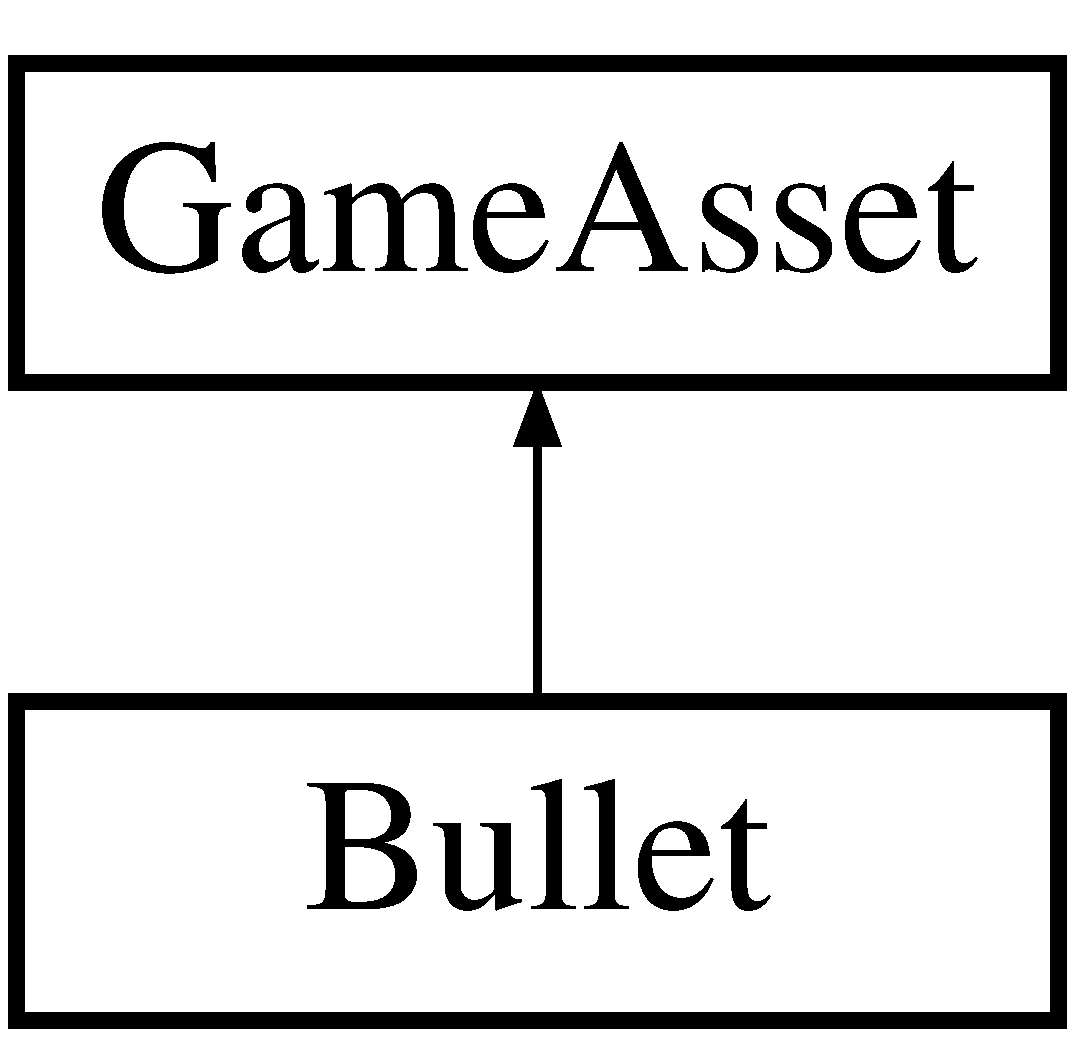
\includegraphics[height=2.000000cm]{classBullet}
\end{center}
\end{figure}
\subsection*{Public Member Functions}
\begin{DoxyCompactItemize}
\item 
\hyperlink{classBullet_acd7befc0bc18907cc1d871d37bbdddeb}{Bullet} ()
\item 
\hyperlink{classBullet_aead3bc218cbfec02093a0546bef197d6}{Bullet} (float x, float y, float z)
\item 
\hyperlink{classBullet_aaeb5cb41d7db89f49007b08b41f1bfcf}{$\sim$\-Bullet} ()
\item 
virtual void \hyperlink{classBullet_a32f4a0611fe2dd245fee955d14ca1f68}{update} ()
\item 
virtual void \hyperlink{classBullet_a3912974232447f64002fd657340a7b3b}{draw} ()
\item 
virtual void \hyperlink{classBullet_a1a4ffaed3fe46e010bb981ebbbd38ecd}{clean} ()
\end{DoxyCompactItemize}
\subsection*{Additional Inherited Members}


\subsection{Detailed Description}


Definition at line 6 of file Bullet.\-h.



\subsection{Constructor \& Destructor Documentation}
\hypertarget{classBullet_acd7befc0bc18907cc1d871d37bbdddeb}{\index{Bullet@{Bullet}!Bullet@{Bullet}}
\index{Bullet@{Bullet}!Bullet@{Bullet}}
\subsubsection[{Bullet}]{\setlength{\rightskip}{0pt plus 5cm}Bullet\-::\-Bullet (
\begin{DoxyParamCaption}
{}
\end{DoxyParamCaption}
)}}\label{classBullet_acd7befc0bc18907cc1d871d37bbdddeb}


Definition at line 3 of file Bullet.\-cpp.


\begin{DoxyCode}
4   : \hyperlink{classGameAsset_a9c96b0bafa2b6973a2e8c09bf51c52ec}{GameAsset}(
5           \textcolor{keywordtype}{string}(\textcolor{stringliteral}{"CubeRacer/shaders/hello-gl.v.glsl"})
6           , \textcolor{keywordtype}{string}(\textcolor{stringliteral}{"CubeRacer/shaders/hello-gl.f.glsl"})
7           )
8 \{
9   \hyperlink{classBullet_acd7befc0bc18907cc1d871d37bbdddeb}{Bullet}(0, 0, 0);
10 \}
\end{DoxyCode}
\hypertarget{classBullet_aead3bc218cbfec02093a0546bef197d6}{\index{Bullet@{Bullet}!Bullet@{Bullet}}
\index{Bullet@{Bullet}!Bullet@{Bullet}}
\subsubsection[{Bullet}]{\setlength{\rightskip}{0pt plus 5cm}Bullet\-::\-Bullet (
\begin{DoxyParamCaption}
\item[{float}]{x, }
\item[{float}]{y, }
\item[{float}]{z}
\end{DoxyParamCaption}
)}}\label{classBullet_aead3bc218cbfec02093a0546bef197d6}


Definition at line 12 of file Bullet.\-cpp.


\begin{DoxyCode}
12                                         \{
13 
14   \textcolor{comment}{// A default "unit" triangular pyramid}
15   \hyperlink{classGameAsset_a3e8d7dc58d3d4efafbbce1536b78dbc7}{num\_vertices} = 5;
16   \hyperlink{classGameAsset_aae4d864335c2eca685cc86602881cd18}{num\_triangles} = 6;
17   \hyperlink{classGameAsset_ae1d682ecf84d9cd3f91a8c870acf2777}{g\_vertex\_buffer\_data} = \textcolor{keyword}{new} GLfloat[\hyperlink{classGameAsset_a3e8d7dc58d3d4efafbbce1536b78dbc7}{num\_vertices} * 3]; \textcolor{comment}{// three points per
       vertex}
18   \hyperlink{classGameAsset_ab859393c9158c8bda39cd100475fee25}{g\_element\_buffer\_data} = \textcolor{keyword}{new} GLushort[\hyperlink{classGameAsset_aae4d864335c2eca685cc86602881cd18}{num\_triangles} * 3]; \textcolor{comment}{// three
       vertices per triangle}
19 
20   \hyperlink{classGameAsset_ae1d682ecf84d9cd3f91a8c870acf2777}{g\_vertex\_buffer\_data}[0]  = -0.125; \textcolor{comment}{//Bottom Left Point 0}
21   \hyperlink{classGameAsset_ae1d682ecf84d9cd3f91a8c870acf2777}{g\_vertex\_buffer\_data}[1]  = -0.125;
22   \hyperlink{classGameAsset_ae1d682ecf84d9cd3f91a8c870acf2777}{g\_vertex\_buffer\_data}[2]  = -0.25;
23 
24   \hyperlink{classGameAsset_ae1d682ecf84d9cd3f91a8c870acf2777}{g\_vertex\_buffer\_data}[3]  =  0.125;  \textcolor{comment}{//Bottom Right Point 1}
25   \hyperlink{classGameAsset_ae1d682ecf84d9cd3f91a8c870acf2777}{g\_vertex\_buffer\_data}[4]  = -0.125;
26   \hyperlink{classGameAsset_ae1d682ecf84d9cd3f91a8c870acf2777}{g\_vertex\_buffer\_data}[5]  = -0.25;
27 
28   \hyperlink{classGameAsset_ae1d682ecf84d9cd3f91a8c870acf2777}{g\_vertex\_buffer\_data}[6]  = -0.125;  \textcolor{comment}{//Top Left Point 2}
29   \hyperlink{classGameAsset_ae1d682ecf84d9cd3f91a8c870acf2777}{g\_vertex\_buffer\_data}[7]  =  0.125;
30   \hyperlink{classGameAsset_ae1d682ecf84d9cd3f91a8c870acf2777}{g\_vertex\_buffer\_data}[8]  = -0.25;
31 
32   \hyperlink{classGameAsset_ae1d682ecf84d9cd3f91a8c870acf2777}{g\_vertex\_buffer\_data}[9]  =  0.125;  \textcolor{comment}{//Top Right Point 3}
33   \hyperlink{classGameAsset_ae1d682ecf84d9cd3f91a8c870acf2777}{g\_vertex\_buffer\_data}[10] =  0.125;
34   \hyperlink{classGameAsset_ae1d682ecf84d9cd3f91a8c870acf2777}{g\_vertex\_buffer\_data}[11] = -0.25;
35  
36   \hyperlink{classGameAsset_ae1d682ecf84d9cd3f91a8c870acf2777}{g\_vertex\_buffer\_data}[12] =  0.0;  \textcolor{comment}{//Front point 4}
37   \hyperlink{classGameAsset_ae1d682ecf84d9cd3f91a8c870acf2777}{g\_vertex\_buffer\_data}[13] =  0.0;
38   \hyperlink{classGameAsset_ae1d682ecf84d9cd3f91a8c870acf2777}{g\_vertex\_buffer\_data}[14] =  0.5;
39 
40   \hyperlink{classGameAsset_ab859393c9158c8bda39cd100475fee25}{g\_element\_buffer\_data}[0]  = 0;
41   \hyperlink{classGameAsset_ab859393c9158c8bda39cd100475fee25}{g\_element\_buffer\_data}[1]  = 1;
42   \hyperlink{classGameAsset_ab859393c9158c8bda39cd100475fee25}{g\_element\_buffer\_data}[2]  = 2;
43 
44   \hyperlink{classGameAsset_ab859393c9158c8bda39cd100475fee25}{g\_element\_buffer\_data}[3]  = 1;
45   \hyperlink{classGameAsset_ab859393c9158c8bda39cd100475fee25}{g\_element\_buffer\_data}[4]  = 3;
46   \hyperlink{classGameAsset_ab859393c9158c8bda39cd100475fee25}{g\_element\_buffer\_data}[5]  = 2;
47 
48   \hyperlink{classGameAsset_ab859393c9158c8bda39cd100475fee25}{g\_element\_buffer\_data}[6]  = 2;
49   \hyperlink{classGameAsset_ab859393c9158c8bda39cd100475fee25}{g\_element\_buffer\_data}[7]  = 3;
50   \hyperlink{classGameAsset_ab859393c9158c8bda39cd100475fee25}{g\_element\_buffer\_data}[8]  = 4;
51 
52   \hyperlink{classGameAsset_ab859393c9158c8bda39cd100475fee25}{g\_element\_buffer\_data}[9]  = 3;
53   \hyperlink{classGameAsset_ab859393c9158c8bda39cd100475fee25}{g\_element\_buffer\_data}[10] = 1;
54   \hyperlink{classGameAsset_ab859393c9158c8bda39cd100475fee25}{g\_element\_buffer\_data}[11] = 4;
55 
56   \hyperlink{classGameAsset_ab859393c9158c8bda39cd100475fee25}{g\_element\_buffer\_data}[12] = 1;
57   \hyperlink{classGameAsset_ab859393c9158c8bda39cd100475fee25}{g\_element\_buffer\_data}[13] = 0;
58   \hyperlink{classGameAsset_ab859393c9158c8bda39cd100475fee25}{g\_element\_buffer\_data}[14] = 4;
59 
60   \hyperlink{classGameAsset_ab859393c9158c8bda39cd100475fee25}{g\_element\_buffer\_data}[15] = 0;
61   \hyperlink{classGameAsset_ab859393c9158c8bda39cd100475fee25}{g\_element\_buffer\_data}[16] = 2;
62   \hyperlink{classGameAsset_ab859393c9158c8bda39cd100475fee25}{g\_element\_buffer\_data}[17] = 4;
63 
64   \hyperlink{classGameAsset_a3444a096fed505b1740bedc95e2cfa6c}{bbox}.reset();
65   \hyperlink{classGameAsset_a3444a096fed505b1740bedc95e2cfa6c}{bbox} = shared\_ptr<BoundingBox>(\textcolor{keyword}{new} \hyperlink{classBoundingBox}{BoundingBox}(\hyperlink{classVectormath_1_1Aos_1_1Point3}{Point3}(x, y, z), 0.5, 0.5, 0.5));
66 
67   \hyperlink{classGameAsset_aa26d85233ece476d599adf90074e9568}{make\_resources}();
68 \}
\end{DoxyCode}
\hypertarget{classBullet_aaeb5cb41d7db89f49007b08b41f1bfcf}{\index{Bullet@{Bullet}!$\sim$\-Bullet@{$\sim$\-Bullet}}
\index{$\sim$\-Bullet@{$\sim$\-Bullet}!Bullet@{Bullet}}
\subsubsection[{$\sim$\-Bullet}]{\setlength{\rightskip}{0pt plus 5cm}Bullet\-::$\sim$\-Bullet (
\begin{DoxyParamCaption}
{}
\end{DoxyParamCaption}
)}}\label{classBullet_aaeb5cb41d7db89f49007b08b41f1bfcf}


Definition at line 70 of file Bullet.\-cpp.


\begin{DoxyCode}
70                 \{
71   \textcolor{comment}{// TODO: do something nice here.}
72 \}
\end{DoxyCode}


\subsection{Member Function Documentation}
\hypertarget{classBullet_a1a4ffaed3fe46e010bb981ebbbd38ecd}{\index{Bullet@{Bullet}!clean@{clean}}
\index{clean@{clean}!Bullet@{Bullet}}
\subsubsection[{clean}]{\setlength{\rightskip}{0pt plus 5cm}void Bullet\-::clean (
\begin{DoxyParamCaption}
{}
\end{DoxyParamCaption}
)\hspace{0.3cm}{\ttfamily [virtual]}}}\label{classBullet_a1a4ffaed3fe46e010bb981ebbbd38ecd}


Implements \hyperlink{classGameAsset_abbea962eaa63a813949b834778b7483e}{Game\-Asset}.



Definition at line 89 of file Bullet.\-cpp.


\begin{DoxyCode}
89 \{ \}
\end{DoxyCode}
\hypertarget{classBullet_a3912974232447f64002fd657340a7b3b}{\index{Bullet@{Bullet}!draw@{draw}}
\index{draw@{draw}!Bullet@{Bullet}}
\subsubsection[{draw}]{\setlength{\rightskip}{0pt plus 5cm}void Bullet\-::draw (
\begin{DoxyParamCaption}
{}
\end{DoxyParamCaption}
)\hspace{0.3cm}{\ttfamily [virtual]}}}\label{classBullet_a3912974232447f64002fd657340a7b3b}


Reimplemented from \hyperlink{classGameAsset_a2d7e18a8f1dd8ba89ed1bd14f2affeab}{Game\-Asset}.



Definition at line 84 of file Bullet.\-cpp.


\begin{DoxyCode}
84                   \{
85 \textcolor{comment}{//  std::cout << "x: " << bbox->getCentre()->getX() << "\(\backslash\)ty: " << bbox->getCentre()->getY() << "\(\backslash\)tz:" <<
       bbox->getCentre()->getZ() << std::endl;}
86   \hyperlink{classGameAsset_a2d7e18a8f1dd8ba89ed1bd14f2affeab}{GameAsset::draw}();
87 \}
\end{DoxyCode}
\hypertarget{classBullet_a32f4a0611fe2dd245fee955d14ca1f68}{\index{Bullet@{Bullet}!update@{update}}
\index{update@{update}!Bullet@{Bullet}}
\subsubsection[{update}]{\setlength{\rightskip}{0pt plus 5cm}void Bullet\-::update (
\begin{DoxyParamCaption}
{}
\end{DoxyParamCaption}
)\hspace{0.3cm}{\ttfamily [virtual]}}}\label{classBullet_a32f4a0611fe2dd245fee955d14ca1f68}


Implements \hyperlink{classGameAsset_a42688ec8f02e201eaaa01e74a112083f}{Game\-Asset}.



Definition at line 74 of file Bullet.\-cpp.


\begin{DoxyCode}
74                     \{
75 
76   \textcolor{keywordflow}{if} (\hyperlink{classGameAsset_aebf93ae52dc7fabbb6ec7edaadf915d0}{isAlive}) \{
77     shared\_ptr<Point3> p = shared\_ptr<Point3>(\textcolor{keyword}{new} \hyperlink{classVectormath_1_1Aos_1_1Point3}{Point3}(this->\hyperlink{classGameAsset_a3444a096fed505b1740bedc95e2cfa6c}{bbox}->getCentre()->getX(), 0, 
      this->\hyperlink{classGameAsset_a3444a096fed505b1740bedc95e2cfa6c}{bbox}->getCentre()->getZ() + 0.1));
78     this->\hyperlink{classGameAsset_a3444a096fed505b1740bedc95e2cfa6c}{bbox}.reset();
79     this->\hyperlink{classGameAsset_a3444a096fed505b1740bedc95e2cfa6c}{bbox} = shared\_ptr<BoundingBox>(\textcolor{keyword}{new} \hyperlink{classBoundingBox}{BoundingBox}(*p, 0.5, 0.5, 0.5));
80     \textcolor{keywordflow}{if}( this->\hyperlink{classGameAsset_a3444a096fed505b1740bedc95e2cfa6c}{bbox}->getCentre()->getZ() > 25) \{ this->\hyperlink{classGameAsset_a631982e6d36061c08c7e8981ce0fd308}{dead}(); \}
81   \}
82 \}
\end{DoxyCode}


The documentation for this class was generated from the following files\-:\begin{DoxyCompactItemize}
\item 
/home/sam/\-Cube\-Racer/src/\hyperlink{Bullet_8h}{Bullet.\-h}\item 
/home/sam/\-Cube\-Racer/src/\hyperlink{Bullet_8cpp}{Bullet.\-cpp}\end{DoxyCompactItemize}

\hypertarget{classCamera}{\section{Camera Class Reference}
\label{classCamera}\index{Camera@{Camera}}
}


{\ttfamily \#include $<$Camera.\-h$>$}

\subsection*{Public Member Functions}
\begin{DoxyCompactItemize}
\item 
virtual \hyperlink{classCamera_ad1897942d0ccf91052386388a497349f}{$\sim$\-Camera} ()
\item 
void \hyperlink{classCamera_a16c5e6f7b2eed95a78675f55c4a435e6}{set\-Camera} (const \hyperlink{classVectormath_1_1Aos_1_1Matrix4}{Matrix4} \&m)
\item 
void \hyperlink{classCamera_aa91c4a447f23e08322ef17f2786851bf}{look\-At} (const \hyperlink{classVectormath_1_1Aos_1_1Point3}{Point3} \&eye, const \hyperlink{classVectormath_1_1Aos_1_1Point3}{Point3} \&point, const \hyperlink{classVectormath_1_1Aos_1_1Vector3}{Vector3} \&up)
\item 
float $\ast$ \hyperlink{classCamera_a25f2f9d8ccc76f38c0580709587afadf}{get\-Camera} ()
\item 
\hyperlink{classVectormath_1_1Aos_1_1Matrix4}{Matrix4} \& \hyperlink{classCamera_a156b6aba4309cde6f0252ff325663e2f}{get\-Camera\-M} ()
\end{DoxyCompactItemize}
\subsection*{Static Public Member Functions}
\begin{DoxyCompactItemize}
\item 
static \hyperlink{classCamera}{Camera} \& \hyperlink{classCamera_aa84baebe5d771ddfd82a5b55bd3fde39}{get\-Instance} ()
\end{DoxyCompactItemize}


\subsection{Detailed Description}


Definition at line 14 of file Camera.\-h.



\subsection{Constructor \& Destructor Documentation}
\hypertarget{classCamera_ad1897942d0ccf91052386388a497349f}{\index{Camera@{Camera}!$\sim$\-Camera@{$\sim$\-Camera}}
\index{$\sim$\-Camera@{$\sim$\-Camera}!Camera@{Camera}}
\subsubsection[{$\sim$\-Camera}]{\setlength{\rightskip}{0pt plus 5cm}Camera\-::$\sim$\-Camera (
\begin{DoxyParamCaption}
{}
\end{DoxyParamCaption}
)\hspace{0.3cm}{\ttfamily [virtual]}}}\label{classCamera_ad1897942d0ccf91052386388a497349f}


Definition at line 12 of file Camera.\-cpp.


\begin{DoxyCode}
12                 \{
13     \textcolor{comment}{// TODO Auto-generated destructor stub}
14 \}
\end{DoxyCode}


\subsection{Member Function Documentation}
\hypertarget{classCamera_a25f2f9d8ccc76f38c0580709587afadf}{\index{Camera@{Camera}!get\-Camera@{get\-Camera}}
\index{get\-Camera@{get\-Camera}!Camera@{Camera}}
\subsubsection[{get\-Camera}]{\setlength{\rightskip}{0pt plus 5cm}float $\ast$ Camera\-::get\-Camera (
\begin{DoxyParamCaption}
{}
\end{DoxyParamCaption}
)}}\label{classCamera_a25f2f9d8ccc76f38c0580709587afadf}


Definition at line 26 of file Camera.\-cpp.


\begin{DoxyCode}
26                          \{
27     \textcolor{keywordtype}{float} * f = \textcolor{keyword}{new} \textcolor{keywordtype}{float}[16];
28     f[0] = camera->\hyperlink{classVectormath_1_1Aos_1_1Matrix4_a70063e1461d582bf7af3242f14fef9c2}{getCol0}().\hyperlink{classVectormath_1_1Aos_1_1Vector4_af067fb75d2fdf3a88189229131f36329}{getX}();
29     f[4] = camera->\hyperlink{classVectormath_1_1Aos_1_1Matrix4_a70063e1461d582bf7af3242f14fef9c2}{getCol0}().\hyperlink{classVectormath_1_1Aos_1_1Vector4_a895b1271a74265bb853772718aca2b24}{getY}();
30     f[8] = camera->\hyperlink{classVectormath_1_1Aos_1_1Matrix4_a70063e1461d582bf7af3242f14fef9c2}{getCol0}().\hyperlink{classVectormath_1_1Aos_1_1Vector4_a51336902d57b1c54df19fb708e93b4f2}{getZ}();
31     f[12] = camera->\hyperlink{classVectormath_1_1Aos_1_1Matrix4_a70063e1461d582bf7af3242f14fef9c2}{getCol0}().\hyperlink{classVectormath_1_1Aos_1_1Vector4_a775bd40a8bd926cd510d39e890c0b686}{getW}();
32 
33     f[1] = camera->\hyperlink{classVectormath_1_1Aos_1_1Matrix4_af2a346e5671e137e665abf428ea3fe37}{getCol1}().\hyperlink{classVectormath_1_1Aos_1_1Vector4_af067fb75d2fdf3a88189229131f36329}{getX}();
34     f[5] = camera->\hyperlink{classVectormath_1_1Aos_1_1Matrix4_af2a346e5671e137e665abf428ea3fe37}{getCol1}().\hyperlink{classVectormath_1_1Aos_1_1Vector4_a895b1271a74265bb853772718aca2b24}{getY}();
35     f[9] = camera->\hyperlink{classVectormath_1_1Aos_1_1Matrix4_af2a346e5671e137e665abf428ea3fe37}{getCol1}().\hyperlink{classVectormath_1_1Aos_1_1Vector4_a51336902d57b1c54df19fb708e93b4f2}{getZ}();
36     f[13] = camera->\hyperlink{classVectormath_1_1Aos_1_1Matrix4_af2a346e5671e137e665abf428ea3fe37}{getCol1}().\hyperlink{classVectormath_1_1Aos_1_1Vector4_a775bd40a8bd926cd510d39e890c0b686}{getW}();
37 
38     f[2] = camera->\hyperlink{classVectormath_1_1Aos_1_1Matrix4_a578e25e020f032f6797d091d60bd666c}{getCol2}().\hyperlink{classVectormath_1_1Aos_1_1Vector4_af067fb75d2fdf3a88189229131f36329}{getX}();
39     f[6] = camera->\hyperlink{classVectormath_1_1Aos_1_1Matrix4_a578e25e020f032f6797d091d60bd666c}{getCol2}().\hyperlink{classVectormath_1_1Aos_1_1Vector4_a895b1271a74265bb853772718aca2b24}{getY}();
40     f[10] = camera->\hyperlink{classVectormath_1_1Aos_1_1Matrix4_a578e25e020f032f6797d091d60bd666c}{getCol2}().\hyperlink{classVectormath_1_1Aos_1_1Vector4_a51336902d57b1c54df19fb708e93b4f2}{getZ}();
41     f[14] = camera->\hyperlink{classVectormath_1_1Aos_1_1Matrix4_a578e25e020f032f6797d091d60bd666c}{getCol2}().\hyperlink{classVectormath_1_1Aos_1_1Vector4_a775bd40a8bd926cd510d39e890c0b686}{getW}();
42 
43     f[3] = camera->\hyperlink{classVectormath_1_1Aos_1_1Matrix4_afa7a80b51829c7972210d619b764658e}{getCol3}().\hyperlink{classVectormath_1_1Aos_1_1Vector4_af067fb75d2fdf3a88189229131f36329}{getX}();
44     f[7] = camera->\hyperlink{classVectormath_1_1Aos_1_1Matrix4_afa7a80b51829c7972210d619b764658e}{getCol3}().\hyperlink{classVectormath_1_1Aos_1_1Vector4_a895b1271a74265bb853772718aca2b24}{getY}();
45     f[11] = camera->\hyperlink{classVectormath_1_1Aos_1_1Matrix4_afa7a80b51829c7972210d619b764658e}{getCol3}().\hyperlink{classVectormath_1_1Aos_1_1Vector4_a51336902d57b1c54df19fb708e93b4f2}{getZ}();
46     f[15] = camera->\hyperlink{classVectormath_1_1Aos_1_1Matrix4_afa7a80b51829c7972210d619b764658e}{getCol3}().\hyperlink{classVectormath_1_1Aos_1_1Vector4_a775bd40a8bd926cd510d39e890c0b686}{getW}();
47     \textcolor{keywordflow}{return} f;
48 \}
\end{DoxyCode}
\hypertarget{classCamera_a156b6aba4309cde6f0252ff325663e2f}{\index{Camera@{Camera}!get\-Camera\-M@{get\-Camera\-M}}
\index{get\-Camera\-M@{get\-Camera\-M}!Camera@{Camera}}
\subsubsection[{get\-Camera\-M}]{\setlength{\rightskip}{0pt plus 5cm}{\bf Matrix4} \& Camera\-::get\-Camera\-M (
\begin{DoxyParamCaption}
{}
\end{DoxyParamCaption}
)}}\label{classCamera_a156b6aba4309cde6f0252ff325663e2f}


Definition at line 50 of file Camera.\-cpp.


\begin{DoxyCode}
50                             \{
51   \textcolor{keywordflow}{return} *camera;
52 \}
\end{DoxyCode}
\hypertarget{classCamera_aa84baebe5d771ddfd82a5b55bd3fde39}{\index{Camera@{Camera}!get\-Instance@{get\-Instance}}
\index{get\-Instance@{get\-Instance}!Camera@{Camera}}
\subsubsection[{get\-Instance}]{\setlength{\rightskip}{0pt plus 5cm}{\bf Camera} \& Camera\-::get\-Instance (
\begin{DoxyParamCaption}
{}
\end{DoxyParamCaption}
)\hspace{0.3cm}{\ttfamily [static]}}}\label{classCamera_aa84baebe5d771ddfd82a5b55bd3fde39}


Definition at line 54 of file Camera.\-cpp.


\begin{DoxyCode}
54                             \{
55     \textcolor{keywordflow}{if}(0 == c) \{
56         c = \textcolor{keyword}{new} \hyperlink{classCamera}{Camera}();
57     \}
58     \textcolor{keywordflow}{return} (*c);
59 \}
\end{DoxyCode}
\hypertarget{classCamera_aa91c4a447f23e08322ef17f2786851bf}{\index{Camera@{Camera}!look\-At@{look\-At}}
\index{look\-At@{look\-At}!Camera@{Camera}}
\subsubsection[{look\-At}]{\setlength{\rightskip}{0pt plus 5cm}void Camera\-::look\-At (
\begin{DoxyParamCaption}
\item[{const {\bf Point3} \&}]{eye, }
\item[{const {\bf Point3} \&}]{point, }
\item[{const {\bf Vector3} \&}]{up}
\end{DoxyParamCaption}
)}}\label{classCamera_aa91c4a447f23e08322ef17f2786851bf}


Definition at line 16 of file Camera.\-cpp.


\begin{DoxyCode}
16                                                                              \{
17   camera = \textcolor{keyword}{new} \hyperlink{classVectormath_1_1Aos_1_1Matrix4}{Matrix4}(camera->\hyperlink{classVectormath_1_1Aos_1_1Matrix4_a49e313a5abadfcf35efdda1a5276c95a}{lookAt}(eye, point, up));
18 \}
\end{DoxyCode}
\hypertarget{classCamera_a16c5e6f7b2eed95a78675f55c4a435e6}{\index{Camera@{Camera}!set\-Camera@{set\-Camera}}
\index{set\-Camera@{set\-Camera}!Camera@{Camera}}
\subsubsection[{set\-Camera}]{\setlength{\rightskip}{0pt plus 5cm}void Camera\-::set\-Camera (
\begin{DoxyParamCaption}
\item[{const {\bf Matrix4} \&}]{m}
\end{DoxyParamCaption}
)}}\label{classCamera_a16c5e6f7b2eed95a78675f55c4a435e6}


Definition at line 20 of file Camera.\-cpp.


\begin{DoxyCode}
20                                         \{
21   \hyperlink{classVectormath_1_1Aos_1_1Matrix4}{Matrix4} * tmp = camera;
22   camera = \textcolor{keyword}{new} \hyperlink{classVectormath_1_1Aos_1_1Matrix4}{Matrix4}(m);
23   \textcolor{keyword}{delete} (tmp);
24 \}
\end{DoxyCode}


The documentation for this class was generated from the following files\-:\begin{DoxyCompactItemize}
\item 
/home/sam/\-Cube\-Racer/src/\hyperlink{Camera_8h}{Camera.\-h}\item 
/home/sam/\-Cube\-Racer/src/\hyperlink{Camera_8cpp}{Camera.\-cpp}\end{DoxyCompactItemize}

\hypertarget{classCubeAsset}{\section{Cube\-Asset Class Reference}
\label{classCubeAsset}\index{Cube\-Asset@{Cube\-Asset}}
}


{\ttfamily \#include $<$Cube\-Asset.\-h$>$}

Inheritance diagram for Cube\-Asset\-:\begin{figure}[H]
\begin{center}
\leavevmode
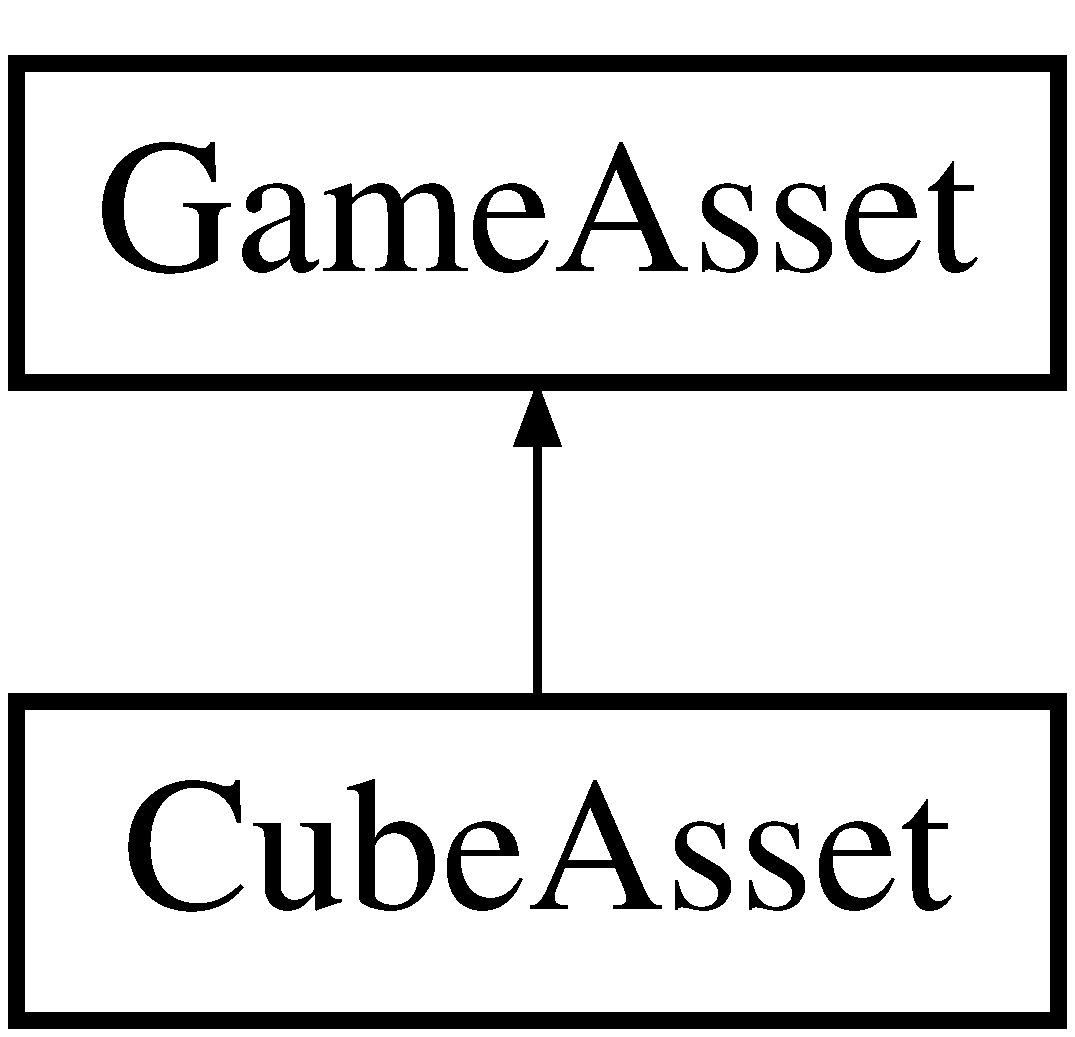
\includegraphics[height=2.000000cm]{classCubeAsset}
\end{center}
\end{figure}
\subsection*{Public Types}
\begin{DoxyCompactItemize}
\item 
enum \hyperlink{classCubeAsset_a26b74931626bfd5877b97363bc0f4404}{vertices} \{ \\*
\hyperlink{classCubeAsset_a26b74931626bfd5877b97363bc0f4404ade8c144c8d334f8f19dce1f1d86f1b4d}{F0}, 
\hyperlink{classCubeAsset_a26b74931626bfd5877b97363bc0f4404a3b9d40699743f0e6043ae3981cdd10b0}{F1}, 
\hyperlink{classCubeAsset_a26b74931626bfd5877b97363bc0f4404a0a7b167f1f8b61902492356eb4852871}{F2}, 
\hyperlink{classCubeAsset_a26b74931626bfd5877b97363bc0f4404a255c0425fbbb033a974a4e6f13678225}{F3}, 
\\*
\hyperlink{classCubeAsset_a26b74931626bfd5877b97363bc0f4404a949b2d4313c2eda31244798e23db7823}{B4}, 
\hyperlink{classCubeAsset_a26b74931626bfd5877b97363bc0f4404a1730ea3a776c19694b4e13208591197a}{B5}, 
\hyperlink{classCubeAsset_a26b74931626bfd5877b97363bc0f4404a3a4204130a8697e0f9df4223cec9b898}{B6}, 
\hyperlink{classCubeAsset_a26b74931626bfd5877b97363bc0f4404ab417aa4f7ad0b19b47a12e546c607e15}{B7}
 \}
\end{DoxyCompactItemize}
\subsection*{Public Member Functions}
\begin{DoxyCompactItemize}
\item 
\hyperlink{classCubeAsset_a2f46c2bbb2453371b7ed97b50125aaf3}{Cube\-Asset} ()
\item 
\hyperlink{classCubeAsset_ad75b73237824794b0822c3404c554523}{Cube\-Asset} (float x, float y, float z)
\item 
\hyperlink{classCubeAsset_ab3ab9a5da82cbf8537a28652410093b1}{$\sim$\-Cube\-Asset} ()
\item 
virtual void \hyperlink{classCubeAsset_a45f15f556999ddb0789eaf01fb0df45d}{update} ()
\item 
virtual void \hyperlink{classCubeAsset_ae986d0b82941b268666f697877530ca5}{draw} ()
\item 
virtual void \hyperlink{classCubeAsset_af158511433013403bc4fe0c13e8577f3}{clean} ()
\end{DoxyCompactItemize}
\subsection*{Additional Inherited Members}


\subsection{Detailed Description}


Definition at line 6 of file Cube\-Asset.\-h.



\subsection{Member Enumeration Documentation}
\hypertarget{classCubeAsset_a26b74931626bfd5877b97363bc0f4404}{\index{Cube\-Asset@{Cube\-Asset}!vertices@{vertices}}
\index{vertices@{vertices}!CubeAsset@{Cube\-Asset}}
\subsubsection[{vertices}]{\setlength{\rightskip}{0pt plus 5cm}enum {\bf Cube\-Asset\-::vertices}}}\label{classCubeAsset_a26b74931626bfd5877b97363bc0f4404}
\begin{Desc}
\item[Enumerator]\par
\begin{description}
\index{F0@{F0}!Cube\-Asset@{Cube\-Asset}}\index{Cube\-Asset@{Cube\-Asset}!F0@{F0}}\item[{\em 
\hypertarget{classCubeAsset_a26b74931626bfd5877b97363bc0f4404ade8c144c8d334f8f19dce1f1d86f1b4d}{F0}\label{classCubeAsset_a26b74931626bfd5877b97363bc0f4404ade8c144c8d334f8f19dce1f1d86f1b4d}
}]\index{F1@{F1}!Cube\-Asset@{Cube\-Asset}}\index{Cube\-Asset@{Cube\-Asset}!F1@{F1}}\item[{\em 
\hypertarget{classCubeAsset_a26b74931626bfd5877b97363bc0f4404a3b9d40699743f0e6043ae3981cdd10b0}{F1}\label{classCubeAsset_a26b74931626bfd5877b97363bc0f4404a3b9d40699743f0e6043ae3981cdd10b0}
}]\index{F2@{F2}!Cube\-Asset@{Cube\-Asset}}\index{Cube\-Asset@{Cube\-Asset}!F2@{F2}}\item[{\em 
\hypertarget{classCubeAsset_a26b74931626bfd5877b97363bc0f4404a0a7b167f1f8b61902492356eb4852871}{F2}\label{classCubeAsset_a26b74931626bfd5877b97363bc0f4404a0a7b167f1f8b61902492356eb4852871}
}]\index{F3@{F3}!Cube\-Asset@{Cube\-Asset}}\index{Cube\-Asset@{Cube\-Asset}!F3@{F3}}\item[{\em 
\hypertarget{classCubeAsset_a26b74931626bfd5877b97363bc0f4404a255c0425fbbb033a974a4e6f13678225}{F3}\label{classCubeAsset_a26b74931626bfd5877b97363bc0f4404a255c0425fbbb033a974a4e6f13678225}
}]\index{B4@{B4}!Cube\-Asset@{Cube\-Asset}}\index{Cube\-Asset@{Cube\-Asset}!B4@{B4}}\item[{\em 
\hypertarget{classCubeAsset_a26b74931626bfd5877b97363bc0f4404a949b2d4313c2eda31244798e23db7823}{B4}\label{classCubeAsset_a26b74931626bfd5877b97363bc0f4404a949b2d4313c2eda31244798e23db7823}
}]\index{B5@{B5}!Cube\-Asset@{Cube\-Asset}}\index{Cube\-Asset@{Cube\-Asset}!B5@{B5}}\item[{\em 
\hypertarget{classCubeAsset_a26b74931626bfd5877b97363bc0f4404a1730ea3a776c19694b4e13208591197a}{B5}\label{classCubeAsset_a26b74931626bfd5877b97363bc0f4404a1730ea3a776c19694b4e13208591197a}
}]\index{B6@{B6}!Cube\-Asset@{Cube\-Asset}}\index{Cube\-Asset@{Cube\-Asset}!B6@{B6}}\item[{\em 
\hypertarget{classCubeAsset_a26b74931626bfd5877b97363bc0f4404a3a4204130a8697e0f9df4223cec9b898}{B6}\label{classCubeAsset_a26b74931626bfd5877b97363bc0f4404a3a4204130a8697e0f9df4223cec9b898}
}]\index{B7@{B7}!Cube\-Asset@{Cube\-Asset}}\index{Cube\-Asset@{Cube\-Asset}!B7@{B7}}\item[{\em 
\hypertarget{classCubeAsset_a26b74931626bfd5877b97363bc0f4404ab417aa4f7ad0b19b47a12e546c607e15}{B7}\label{classCubeAsset_a26b74931626bfd5877b97363bc0f4404ab417aa4f7ad0b19b47a12e546c607e15}
}]\end{description}
\end{Desc}


Definition at line 16 of file Cube\-Asset.\-h.


\begin{DoxyCode}
16                 \{
17       \hyperlink{classCubeAsset_a26b74931626bfd5877b97363bc0f4404ade8c144c8d334f8f19dce1f1d86f1b4d}{F0}, \hyperlink{classCubeAsset_a26b74931626bfd5877b97363bc0f4404a3b9d40699743f0e6043ae3981cdd10b0}{F1}, \hyperlink{classCubeAsset_a26b74931626bfd5877b97363bc0f4404a0a7b167f1f8b61902492356eb4852871}{F2}, \hyperlink{classCubeAsset_a26b74931626bfd5877b97363bc0f4404a255c0425fbbb033a974a4e6f13678225}{F3}, \hyperlink{classCubeAsset_a26b74931626bfd5877b97363bc0f4404a949b2d4313c2eda31244798e23db7823}{B4}, \hyperlink{classCubeAsset_a26b74931626bfd5877b97363bc0f4404a1730ea3a776c19694b4e13208591197a}{B5}, \hyperlink{classCubeAsset_a26b74931626bfd5877b97363bc0f4404a3a4204130a8697e0f9df4223cec9b898}{B6}, \hyperlink{classCubeAsset_a26b74931626bfd5877b97363bc0f4404ab417aa4f7ad0b19b47a12e546c607e15}{B7}, 
18   \};
\end{DoxyCode}


\subsection{Constructor \& Destructor Documentation}
\hypertarget{classCubeAsset_a2f46c2bbb2453371b7ed97b50125aaf3}{\index{Cube\-Asset@{Cube\-Asset}!Cube\-Asset@{Cube\-Asset}}
\index{Cube\-Asset@{Cube\-Asset}!CubeAsset@{Cube\-Asset}}
\subsubsection[{Cube\-Asset}]{\setlength{\rightskip}{0pt plus 5cm}Cube\-Asset\-::\-Cube\-Asset (
\begin{DoxyParamCaption}
{}
\end{DoxyParamCaption}
)}}\label{classCubeAsset_a2f46c2bbb2453371b7ed97b50125aaf3}


Definition at line 3 of file Cube\-Asset.\-cpp.


\begin{DoxyCode}
4   : \hyperlink{classGameAsset_a9c96b0bafa2b6973a2e8c09bf51c52ec}{GameAsset}(
5           \textcolor{keywordtype}{string}(\textcolor{stringliteral}{"CubeRacer/shaders/hello-gl.v.glsl"})
6           , \textcolor{keywordtype}{string}(\textcolor{stringliteral}{"CubeRacer/shaders/hello-gl.f.glsl"})
7           )
8 \{
9   \hyperlink{classCubeAsset_a2f46c2bbb2453371b7ed97b50125aaf3}{CubeAsset}(0, 0, 0);
10 \}
\end{DoxyCode}
\hypertarget{classCubeAsset_ad75b73237824794b0822c3404c554523}{\index{Cube\-Asset@{Cube\-Asset}!Cube\-Asset@{Cube\-Asset}}
\index{Cube\-Asset@{Cube\-Asset}!CubeAsset@{Cube\-Asset}}
\subsubsection[{Cube\-Asset}]{\setlength{\rightskip}{0pt plus 5cm}Cube\-Asset\-::\-Cube\-Asset (
\begin{DoxyParamCaption}
\item[{float}]{x, }
\item[{float}]{y, }
\item[{float}]{z}
\end{DoxyParamCaption}
)}}\label{classCubeAsset_ad75b73237824794b0822c3404c554523}


Definition at line 12 of file Cube\-Asset.\-cpp.


\begin{DoxyCode}
12                                               \{
13 
14   \textcolor{comment}{// A default "unit" cube}
15   \hyperlink{classGameAsset_a3e8d7dc58d3d4efafbbce1536b78dbc7}{num\_vertices} = 8;
16   \hyperlink{classGameAsset_aae4d864335c2eca685cc86602881cd18}{num\_triangles} = 12;
17   \hyperlink{classGameAsset_ae1d682ecf84d9cd3f91a8c870acf2777}{g\_vertex\_buffer\_data} = \textcolor{keyword}{new} GLfloat[\hyperlink{classGameAsset_a3e8d7dc58d3d4efafbbce1536b78dbc7}{num\_vertices} * 3]\{
18 
19   \textcolor{comment}{//     x      y     z}
20     -0.5, -0.5,  0.5, \textcolor{comment}{//F - 0}
21      0.5, -0.5,  0.5, \textcolor{comment}{//F - 1}
22     -0.5,  0.5,  0.5, \textcolor{comment}{//F - 2}
23      0.5,  0.5,  0.5, \textcolor{comment}{//F - 3}
24     -0.5, -0.5, -0.5, \textcolor{comment}{//B - 4}
25      0.5, -0.5, -0.5, \textcolor{comment}{//B - 5}
26     -0.5,  0.5, -0.5, \textcolor{comment}{//B - 6}
27      0.5,  0.5, -0.5  \textcolor{comment}{//B - 7}
28 \}; \textcolor{comment}{// three points per vertex}
29 
30   \hyperlink{classGameAsset_ab859393c9158c8bda39cd100475fee25}{g\_element\_buffer\_data} = \textcolor{keyword}{new} GLushort[\hyperlink{classGameAsset_aae4d864335c2eca685cc86602881cd18}{num\_triangles} * 3]\{
31 
32     \hyperlink{classCubeAsset_a26b74931626bfd5877b97363bc0f4404ade8c144c8d334f8f19dce1f1d86f1b4d}{F0}, \hyperlink{classCubeAsset_a26b74931626bfd5877b97363bc0f4404a3b9d40699743f0e6043ae3981cdd10b0}{F1}, \hyperlink{classCubeAsset_a26b74931626bfd5877b97363bc0f4404a0a7b167f1f8b61902492356eb4852871}{F2},  \textcolor{comment}{//front}
33     \hyperlink{classCubeAsset_a26b74931626bfd5877b97363bc0f4404a3b9d40699743f0e6043ae3981cdd10b0}{F1}, \hyperlink{classCubeAsset_a26b74931626bfd5877b97363bc0f4404a255c0425fbbb033a974a4e6f13678225}{F3}, \hyperlink{classCubeAsset_a26b74931626bfd5877b97363bc0f4404a0a7b167f1f8b61902492356eb4852871}{F2},
34 
35     \hyperlink{classCubeAsset_a26b74931626bfd5877b97363bc0f4404a3b9d40699743f0e6043ae3981cdd10b0}{F1}, \hyperlink{classCubeAsset_a26b74931626bfd5877b97363bc0f4404a1730ea3a776c19694b4e13208591197a}{B5}, \hyperlink{classCubeAsset_a26b74931626bfd5877b97363bc0f4404a255c0425fbbb033a974a4e6f13678225}{F3},  \textcolor{comment}{//right}
36     \hyperlink{classCubeAsset_a26b74931626bfd5877b97363bc0f4404a1730ea3a776c19694b4e13208591197a}{B5}, \hyperlink{classCubeAsset_a26b74931626bfd5877b97363bc0f4404ab417aa4f7ad0b19b47a12e546c607e15}{B7}, \hyperlink{classCubeAsset_a26b74931626bfd5877b97363bc0f4404a255c0425fbbb033a974a4e6f13678225}{F3},
37 
38     \hyperlink{classCubeAsset_a26b74931626bfd5877b97363bc0f4404a1730ea3a776c19694b4e13208591197a}{B5}, \hyperlink{classCubeAsset_a26b74931626bfd5877b97363bc0f4404a949b2d4313c2eda31244798e23db7823}{B4}, \hyperlink{classCubeAsset_a26b74931626bfd5877b97363bc0f4404ab417aa4f7ad0b19b47a12e546c607e15}{B7},  \textcolor{comment}{//back}
39     \hyperlink{classCubeAsset_a26b74931626bfd5877b97363bc0f4404a949b2d4313c2eda31244798e23db7823}{B4}, \hyperlink{classCubeAsset_a26b74931626bfd5877b97363bc0f4404a3a4204130a8697e0f9df4223cec9b898}{B6}, \hyperlink{classCubeAsset_a26b74931626bfd5877b97363bc0f4404ab417aa4f7ad0b19b47a12e546c607e15}{B7},
40 
41     \hyperlink{classCubeAsset_a26b74931626bfd5877b97363bc0f4404a949b2d4313c2eda31244798e23db7823}{B4}, \hyperlink{classCubeAsset_a26b74931626bfd5877b97363bc0f4404ade8c144c8d334f8f19dce1f1d86f1b4d}{F0}, \hyperlink{classCubeAsset_a26b74931626bfd5877b97363bc0f4404a3a4204130a8697e0f9df4223cec9b898}{B6},  \textcolor{comment}{//left}
42     \hyperlink{classCubeAsset_a26b74931626bfd5877b97363bc0f4404ade8c144c8d334f8f19dce1f1d86f1b4d}{F0}, \hyperlink{classCubeAsset_a26b74931626bfd5877b97363bc0f4404a0a7b167f1f8b61902492356eb4852871}{F2}, \hyperlink{classCubeAsset_a26b74931626bfd5877b97363bc0f4404a3a4204130a8697e0f9df4223cec9b898}{B6},
43 
44     \hyperlink{classCubeAsset_a26b74931626bfd5877b97363bc0f4404a0a7b167f1f8b61902492356eb4852871}{F2}, \hyperlink{classCubeAsset_a26b74931626bfd5877b97363bc0f4404a255c0425fbbb033a974a4e6f13678225}{F3}, \hyperlink{classCubeAsset_a26b74931626bfd5877b97363bc0f4404a3a4204130a8697e0f9df4223cec9b898}{B6},  \textcolor{comment}{//top}
45     \hyperlink{classCubeAsset_a26b74931626bfd5877b97363bc0f4404a255c0425fbbb033a974a4e6f13678225}{F3}, \hyperlink{classCubeAsset_a26b74931626bfd5877b97363bc0f4404ab417aa4f7ad0b19b47a12e546c607e15}{B7}, \hyperlink{classCubeAsset_a26b74931626bfd5877b97363bc0f4404a3a4204130a8697e0f9df4223cec9b898}{B6},
46 
47     \hyperlink{classCubeAsset_a26b74931626bfd5877b97363bc0f4404a949b2d4313c2eda31244798e23db7823}{B4}, \hyperlink{classCubeAsset_a26b74931626bfd5877b97363bc0f4404a1730ea3a776c19694b4e13208591197a}{B5}, \hyperlink{classCubeAsset_a26b74931626bfd5877b97363bc0f4404ade8c144c8d334f8f19dce1f1d86f1b4d}{F0},  \textcolor{comment}{//bottom}
48     \hyperlink{classCubeAsset_a26b74931626bfd5877b97363bc0f4404a1730ea3a776c19694b4e13208591197a}{B5}, \hyperlink{classCubeAsset_a26b74931626bfd5877b97363bc0f4404a3b9d40699743f0e6043ae3981cdd10b0}{F1}, F0
49     
50 \}; \textcolor{comment}{// three vertices per triangle}
51 
52   \hyperlink{classGameAsset_a3444a096fed505b1740bedc95e2cfa6c}{bbox}.reset();
53   \hyperlink{classGameAsset_a3444a096fed505b1740bedc95e2cfa6c}{bbox} = shared\_ptr<BoundingBox>(\textcolor{keyword}{new} \hyperlink{classBoundingBox}{BoundingBox}(\hyperlink{classVectormath_1_1Aos_1_1Point3}{Point3}(x, y, z), 1.0, 1.0, 1.0));
54 
55   \hyperlink{classGameAsset_aa26d85233ece476d599adf90074e9568}{make\_resources}();
56 \}
\end{DoxyCode}
\hypertarget{classCubeAsset_ab3ab9a5da82cbf8537a28652410093b1}{\index{Cube\-Asset@{Cube\-Asset}!$\sim$\-Cube\-Asset@{$\sim$\-Cube\-Asset}}
\index{$\sim$\-Cube\-Asset@{$\sim$\-Cube\-Asset}!CubeAsset@{Cube\-Asset}}
\subsubsection[{$\sim$\-Cube\-Asset}]{\setlength{\rightskip}{0pt plus 5cm}Cube\-Asset\-::$\sim$\-Cube\-Asset (
\begin{DoxyParamCaption}
{}
\end{DoxyParamCaption}
)}}\label{classCubeAsset_ab3ab9a5da82cbf8537a28652410093b1}


Definition at line 58 of file Cube\-Asset.\-cpp.


\begin{DoxyCode}
58                       \{
59   \textcolor{comment}{// TODO: do something nice and fun here.}
60 \}
\end{DoxyCode}


\subsection{Member Function Documentation}
\hypertarget{classCubeAsset_af158511433013403bc4fe0c13e8577f3}{\index{Cube\-Asset@{Cube\-Asset}!clean@{clean}}
\index{clean@{clean}!CubeAsset@{Cube\-Asset}}
\subsubsection[{clean}]{\setlength{\rightskip}{0pt plus 5cm}void Cube\-Asset\-::clean (
\begin{DoxyParamCaption}
{}
\end{DoxyParamCaption}
)\hspace{0.3cm}{\ttfamily [virtual]}}}\label{classCubeAsset_af158511433013403bc4fe0c13e8577f3}


Implements \hyperlink{classGameAsset_abbea962eaa63a813949b834778b7483e}{Game\-Asset}.



Definition at line 70 of file Cube\-Asset.\-cpp.


\begin{DoxyCode}
70 \{ \} 
\end{DoxyCode}
\hypertarget{classCubeAsset_ae986d0b82941b268666f697877530ca5}{\index{Cube\-Asset@{Cube\-Asset}!draw@{draw}}
\index{draw@{draw}!CubeAsset@{Cube\-Asset}}
\subsubsection[{draw}]{\setlength{\rightskip}{0pt plus 5cm}void Cube\-Asset\-::draw (
\begin{DoxyParamCaption}
{}
\end{DoxyParamCaption}
)\hspace{0.3cm}{\ttfamily [virtual]}}}\label{classCubeAsset_ae986d0b82941b268666f697877530ca5}


Reimplemented from \hyperlink{classGameAsset_a2d7e18a8f1dd8ba89ed1bd14f2affeab}{Game\-Asset}.



Definition at line 65 of file Cube\-Asset.\-cpp.


\begin{DoxyCode}
65                      \{
66 \textcolor{comment}{//  std::cout << "x: " << bbox->getCentre()->getX() << "\(\backslash\)ty: " << bbox->getCentre()->getY() << "\(\backslash\)tz:" <<
       bbox->getCentre()->getZ() << std::endl;}
67   \hyperlink{classGameAsset_a2d7e18a8f1dd8ba89ed1bd14f2affeab}{GameAsset::draw}();
68 \}
\end{DoxyCode}
\hypertarget{classCubeAsset_a45f15f556999ddb0789eaf01fb0df45d}{\index{Cube\-Asset@{Cube\-Asset}!update@{update}}
\index{update@{update}!CubeAsset@{Cube\-Asset}}
\subsubsection[{update}]{\setlength{\rightskip}{0pt plus 5cm}void Cube\-Asset\-::update (
\begin{DoxyParamCaption}
{}
\end{DoxyParamCaption}
)\hspace{0.3cm}{\ttfamily [virtual]}}}\label{classCubeAsset_a45f15f556999ddb0789eaf01fb0df45d}


Implements \hyperlink{classGameAsset_a42688ec8f02e201eaaa01e74a112083f}{Game\-Asset}.



Definition at line 62 of file Cube\-Asset.\-cpp.


\begin{DoxyCode}
62                        \{
63 \}
\end{DoxyCode}


The documentation for this class was generated from the following files\-:\begin{DoxyCompactItemize}
\item 
/home/sam/\-Cube\-Racer/src/\hyperlink{CubeAsset_8h}{Cube\-Asset.\-h}\item 
/home/sam/\-Cube\-Racer/src/\hyperlink{CubeAsset_8cpp}{Cube\-Asset.\-cpp}\end{DoxyCompactItemize}

\hypertarget{classEnemy}{\section{Enemy Class Reference}
\label{classEnemy}\index{Enemy@{Enemy}}
}


{\ttfamily \#include $<$Enemy.\-h$>$}

Inheritance diagram for Enemy\-:\begin{figure}[H]
\begin{center}
\leavevmode
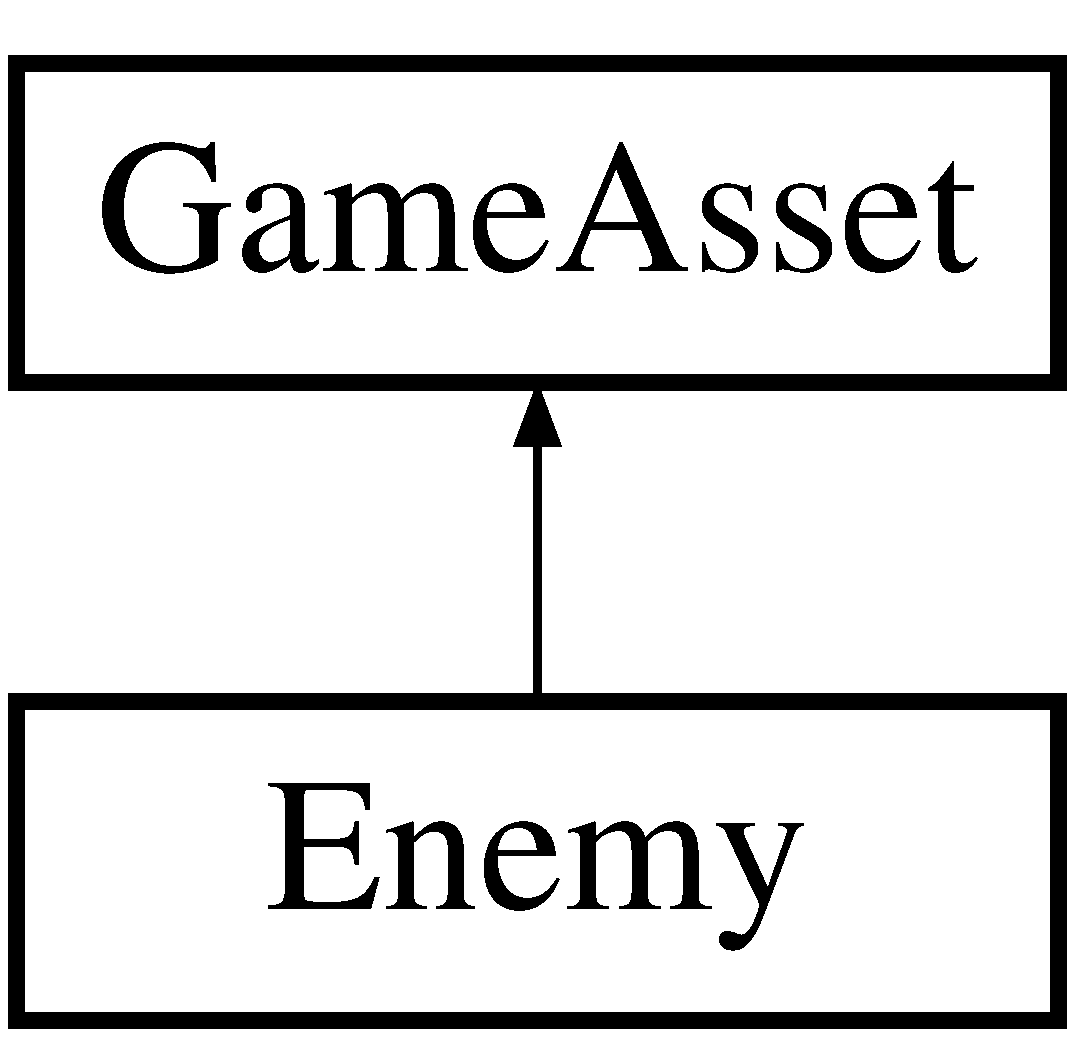
\includegraphics[height=2.000000cm]{classEnemy}
\end{center}
\end{figure}
\subsection*{Public Types}
\begin{DoxyCompactItemize}
\item 
enum \hyperlink{classEnemy_a60fed95ba2edb2a005487c91711fe7d1}{vertices} \{ \\*
\hyperlink{classEnemy_a60fed95ba2edb2a005487c91711fe7d1a27984980bad3e49e3a78994281d6949b}{F0}, 
\hyperlink{classEnemy_a60fed95ba2edb2a005487c91711fe7d1ab95fca6d288fdaa674e85ae46e366e2d}{F1}, 
\hyperlink{classEnemy_a60fed95ba2edb2a005487c91711fe7d1abef72d551f5d130fd850384d075a27d2}{F2}, 
\hyperlink{classEnemy_a60fed95ba2edb2a005487c91711fe7d1a28b74a906d078973f1d59203d964c045}{F3}, 
\\*
\hyperlink{classEnemy_a60fed95ba2edb2a005487c91711fe7d1a32ab5408a61c9a05baada047eaceb025}{B4}, 
\hyperlink{classEnemy_a60fed95ba2edb2a005487c91711fe7d1a00ceaccae0110cd22f3d466348cda9e0}{B5}, 
\hyperlink{classEnemy_a60fed95ba2edb2a005487c91711fe7d1a0822565cdeeb34f9027775bab8f9ae0a}{B6}, 
\hyperlink{classEnemy_a60fed95ba2edb2a005487c91711fe7d1a5ab58c1a775f2759b6bd7fc6f97515df}{B7}
 \}
\end{DoxyCompactItemize}
\subsection*{Public Member Functions}
\begin{DoxyCompactItemize}
\item 
\hyperlink{classEnemy_a94f30d348b6d2840fd71675472ba38dd}{Enemy} ()
\item 
\hyperlink{classEnemy_a53db9778244c976f711f25463982cad2}{Enemy} (float x, float y, float z)
\item 
\hyperlink{classEnemy_ac0eec4755e28c02688065f9657150ac3}{$\sim$\-Enemy} ()
\item 
bool \hyperlink{classEnemy_a0fd40f508e31be597eab5840df775749}{collides\-With} (\hyperlink{classPlayer}{Player} \&a)
\item 
virtual void \hyperlink{classEnemy_ad55ee71b5a8c23fbd00b3c368b90cc64}{update} ()
\item 
virtual void \hyperlink{classEnemy_a7dcf45915f6288ef9264ec60af621b6c}{draw} ()
\item 
virtual void \hyperlink{classEnemy_a12e87c9cb633fed1d846a61cfe7f91c7}{clean} ()
\item 
virtual void \hyperlink{classEnemy_a9a0377be732b07f337206077c1f1acf7}{set\-Diff} (double diff)
\item 
virtual double \hyperlink{classEnemy_ac9934ae427de817275472e64cf617c39}{get\-Diff} ()
\end{DoxyCompactItemize}
\subsection*{Public Attributes}
\begin{DoxyCompactItemize}
\item 
double \hyperlink{classEnemy_acca04a63f878d07a3db3285f5f8fbbed}{difficulty}
\end{DoxyCompactItemize}
\subsection*{Additional Inherited Members}


\subsection{Detailed Description}


Definition at line 7 of file Enemy.\-h.



\subsection{Member Enumeration Documentation}
\hypertarget{classEnemy_a60fed95ba2edb2a005487c91711fe7d1}{\index{Enemy@{Enemy}!vertices@{vertices}}
\index{vertices@{vertices}!Enemy@{Enemy}}
\subsubsection[{vertices}]{\setlength{\rightskip}{0pt plus 5cm}enum {\bf Enemy\-::vertices}}}\label{classEnemy_a60fed95ba2edb2a005487c91711fe7d1}
\begin{Desc}
\item[Enumerator]\par
\begin{description}
\index{F0@{F0}!Enemy@{Enemy}}\index{Enemy@{Enemy}!F0@{F0}}\item[{\em 
\hypertarget{classEnemy_a60fed95ba2edb2a005487c91711fe7d1a27984980bad3e49e3a78994281d6949b}{F0}\label{classEnemy_a60fed95ba2edb2a005487c91711fe7d1a27984980bad3e49e3a78994281d6949b}
}]\index{F1@{F1}!Enemy@{Enemy}}\index{Enemy@{Enemy}!F1@{F1}}\item[{\em 
\hypertarget{classEnemy_a60fed95ba2edb2a005487c91711fe7d1ab95fca6d288fdaa674e85ae46e366e2d}{F1}\label{classEnemy_a60fed95ba2edb2a005487c91711fe7d1ab95fca6d288fdaa674e85ae46e366e2d}
}]\index{F2@{F2}!Enemy@{Enemy}}\index{Enemy@{Enemy}!F2@{F2}}\item[{\em 
\hypertarget{classEnemy_a60fed95ba2edb2a005487c91711fe7d1abef72d551f5d130fd850384d075a27d2}{F2}\label{classEnemy_a60fed95ba2edb2a005487c91711fe7d1abef72d551f5d130fd850384d075a27d2}
}]\index{F3@{F3}!Enemy@{Enemy}}\index{Enemy@{Enemy}!F3@{F3}}\item[{\em 
\hypertarget{classEnemy_a60fed95ba2edb2a005487c91711fe7d1a28b74a906d078973f1d59203d964c045}{F3}\label{classEnemy_a60fed95ba2edb2a005487c91711fe7d1a28b74a906d078973f1d59203d964c045}
}]\index{B4@{B4}!Enemy@{Enemy}}\index{Enemy@{Enemy}!B4@{B4}}\item[{\em 
\hypertarget{classEnemy_a60fed95ba2edb2a005487c91711fe7d1a32ab5408a61c9a05baada047eaceb025}{B4}\label{classEnemy_a60fed95ba2edb2a005487c91711fe7d1a32ab5408a61c9a05baada047eaceb025}
}]\index{B5@{B5}!Enemy@{Enemy}}\index{Enemy@{Enemy}!B5@{B5}}\item[{\em 
\hypertarget{classEnemy_a60fed95ba2edb2a005487c91711fe7d1a00ceaccae0110cd22f3d466348cda9e0}{B5}\label{classEnemy_a60fed95ba2edb2a005487c91711fe7d1a00ceaccae0110cd22f3d466348cda9e0}
}]\index{B6@{B6}!Enemy@{Enemy}}\index{Enemy@{Enemy}!B6@{B6}}\item[{\em 
\hypertarget{classEnemy_a60fed95ba2edb2a005487c91711fe7d1a0822565cdeeb34f9027775bab8f9ae0a}{B6}\label{classEnemy_a60fed95ba2edb2a005487c91711fe7d1a0822565cdeeb34f9027775bab8f9ae0a}
}]\index{B7@{B7}!Enemy@{Enemy}}\index{Enemy@{Enemy}!B7@{B7}}\item[{\em 
\hypertarget{classEnemy_a60fed95ba2edb2a005487c91711fe7d1a5ab58c1a775f2759b6bd7fc6f97515df}{B7}\label{classEnemy_a60fed95ba2edb2a005487c91711fe7d1a5ab58c1a775f2759b6bd7fc6f97515df}
}]\end{description}
\end{Desc}


Definition at line 23 of file Enemy.\-h.


\begin{DoxyCode}
23                 \{
24     \hyperlink{classEnemy_a60fed95ba2edb2a005487c91711fe7d1a27984980bad3e49e3a78994281d6949b}{F0}, \hyperlink{classEnemy_a60fed95ba2edb2a005487c91711fe7d1ab95fca6d288fdaa674e85ae46e366e2d}{F1}, \hyperlink{classEnemy_a60fed95ba2edb2a005487c91711fe7d1abef72d551f5d130fd850384d075a27d2}{F2}, \hyperlink{classEnemy_a60fed95ba2edb2a005487c91711fe7d1a28b74a906d078973f1d59203d964c045}{F3}, \hyperlink{classEnemy_a60fed95ba2edb2a005487c91711fe7d1a32ab5408a61c9a05baada047eaceb025}{B4}, \hyperlink{classEnemy_a60fed95ba2edb2a005487c91711fe7d1a00ceaccae0110cd22f3d466348cda9e0}{B5}, \hyperlink{classEnemy_a60fed95ba2edb2a005487c91711fe7d1a0822565cdeeb34f9027775bab8f9ae0a}{B6}, \hyperlink{classEnemy_a60fed95ba2edb2a005487c91711fe7d1a5ab58c1a775f2759b6bd7fc6f97515df}{B7},
25   \};
\end{DoxyCode}


\subsection{Constructor \& Destructor Documentation}
\hypertarget{classEnemy_a94f30d348b6d2840fd71675472ba38dd}{\index{Enemy@{Enemy}!Enemy@{Enemy}}
\index{Enemy@{Enemy}!Enemy@{Enemy}}
\subsubsection[{Enemy}]{\setlength{\rightskip}{0pt plus 5cm}Enemy\-::\-Enemy (
\begin{DoxyParamCaption}
{}
\end{DoxyParamCaption}
)}}\label{classEnemy_a94f30d348b6d2840fd71675472ba38dd}


Definition at line 3 of file Enemy.\-cpp.


\begin{DoxyCode}
4   : \hyperlink{classGameAsset_a9c96b0bafa2b6973a2e8c09bf51c52ec}{GameAsset}(
5           \textcolor{keywordtype}{string}(\textcolor{stringliteral}{"CubeRacer/shaders/hello-gl.v.glsl"})
6           , \textcolor{keywordtype}{string}(\textcolor{stringliteral}{"CubeRacer/shaders/enemy-gl.f.glsl"})
7           )
8 \{
9   \hyperlink{classEnemy_a94f30d348b6d2840fd71675472ba38dd}{Enemy}(0, 0, 0);
10 \}
\end{DoxyCode}
\hypertarget{classEnemy_a53db9778244c976f711f25463982cad2}{\index{Enemy@{Enemy}!Enemy@{Enemy}}
\index{Enemy@{Enemy}!Enemy@{Enemy}}
\subsubsection[{Enemy}]{\setlength{\rightskip}{0pt plus 5cm}Enemy\-::\-Enemy (
\begin{DoxyParamCaption}
\item[{float}]{x, }
\item[{float}]{y, }
\item[{float}]{z}
\end{DoxyParamCaption}
)}}\label{classEnemy_a53db9778244c976f711f25463982cad2}


Definition at line 12 of file Enemy.\-cpp.


\begin{DoxyCode}
13   : \hyperlink{classGameAsset_a9c96b0bafa2b6973a2e8c09bf51c52ec}{GameAsset}(
14       \textcolor{keywordtype}{string}(\textcolor{stringliteral}{"CubeRacer/shaders/hello-gl.v.glsl"}), 
15       \textcolor{keywordtype}{string}(\textcolor{stringliteral}{"CubeRacer/shaders/enemy-gl.f.glsl"})
16 ) \{
17 
18   \textcolor{comment}{// A default "unit" cube}
19   \hyperlink{classGameAsset_a3e8d7dc58d3d4efafbbce1536b78dbc7}{num\_vertices} = 8;
20   \hyperlink{classGameAsset_aae4d864335c2eca685cc86602881cd18}{num\_triangles} = 12;
21   \hyperlink{classGameAsset_ae1d682ecf84d9cd3f91a8c870acf2777}{g\_vertex\_buffer\_data} = \textcolor{keyword}{new} GLfloat[\hyperlink{classGameAsset_a3e8d7dc58d3d4efafbbce1536b78dbc7}{num\_vertices} * 3]\{
22 
23   \textcolor{comment}{//     x      y     z}
24     -0.5, -0.5,  0.5, \textcolor{comment}{//F - 0}
25      0.5, -0.5,  0.5, \textcolor{comment}{//F - 1}
26     -0.5,  0.5,  0.5, \textcolor{comment}{//F - 2}
27      0.5,  0.5,  0.5, \textcolor{comment}{//F - 3}
28     -0.5, -0.5, -0.5, \textcolor{comment}{//B - 4}
29      0.5, -0.5, -0.5, \textcolor{comment}{//B - 5}
30     -0.5,  0.5, -0.5, \textcolor{comment}{//B - 6}
31      0.5,  0.5, -0.5  \textcolor{comment}{//B - 7}
32 \}; \textcolor{comment}{// three points per vertex}
33 
34   \hyperlink{classGameAsset_ab859393c9158c8bda39cd100475fee25}{g\_element\_buffer\_data} = \textcolor{keyword}{new} GLushort[\hyperlink{classGameAsset_aae4d864335c2eca685cc86602881cd18}{num\_triangles} * 3]\{
35 
36     \hyperlink{classEnemy_a60fed95ba2edb2a005487c91711fe7d1a27984980bad3e49e3a78994281d6949b}{F0}, \hyperlink{classEnemy_a60fed95ba2edb2a005487c91711fe7d1ab95fca6d288fdaa674e85ae46e366e2d}{F1}, \hyperlink{classEnemy_a60fed95ba2edb2a005487c91711fe7d1abef72d551f5d130fd850384d075a27d2}{F2},  \textcolor{comment}{//front}
37     \hyperlink{classEnemy_a60fed95ba2edb2a005487c91711fe7d1ab95fca6d288fdaa674e85ae46e366e2d}{F1}, \hyperlink{classEnemy_a60fed95ba2edb2a005487c91711fe7d1a28b74a906d078973f1d59203d964c045}{F3}, \hyperlink{classEnemy_a60fed95ba2edb2a005487c91711fe7d1abef72d551f5d130fd850384d075a27d2}{F2},
38 
39     \hyperlink{classEnemy_a60fed95ba2edb2a005487c91711fe7d1ab95fca6d288fdaa674e85ae46e366e2d}{F1}, \hyperlink{classEnemy_a60fed95ba2edb2a005487c91711fe7d1a00ceaccae0110cd22f3d466348cda9e0}{B5}, \hyperlink{classEnemy_a60fed95ba2edb2a005487c91711fe7d1a28b74a906d078973f1d59203d964c045}{F3},  \textcolor{comment}{//right}
40     \hyperlink{classEnemy_a60fed95ba2edb2a005487c91711fe7d1a00ceaccae0110cd22f3d466348cda9e0}{B5}, \hyperlink{classEnemy_a60fed95ba2edb2a005487c91711fe7d1a5ab58c1a775f2759b6bd7fc6f97515df}{B7}, \hyperlink{classEnemy_a60fed95ba2edb2a005487c91711fe7d1a28b74a906d078973f1d59203d964c045}{F3},
41 
42     \hyperlink{classEnemy_a60fed95ba2edb2a005487c91711fe7d1a00ceaccae0110cd22f3d466348cda9e0}{B5}, \hyperlink{classEnemy_a60fed95ba2edb2a005487c91711fe7d1a32ab5408a61c9a05baada047eaceb025}{B4}, \hyperlink{classEnemy_a60fed95ba2edb2a005487c91711fe7d1a5ab58c1a775f2759b6bd7fc6f97515df}{B7},  \textcolor{comment}{//back}
43     \hyperlink{classEnemy_a60fed95ba2edb2a005487c91711fe7d1a32ab5408a61c9a05baada047eaceb025}{B4}, \hyperlink{classEnemy_a60fed95ba2edb2a005487c91711fe7d1a0822565cdeeb34f9027775bab8f9ae0a}{B6}, \hyperlink{classEnemy_a60fed95ba2edb2a005487c91711fe7d1a5ab58c1a775f2759b6bd7fc6f97515df}{B7},
44 
45     \hyperlink{classEnemy_a60fed95ba2edb2a005487c91711fe7d1a32ab5408a61c9a05baada047eaceb025}{B4}, \hyperlink{classEnemy_a60fed95ba2edb2a005487c91711fe7d1a27984980bad3e49e3a78994281d6949b}{F0}, \hyperlink{classEnemy_a60fed95ba2edb2a005487c91711fe7d1a0822565cdeeb34f9027775bab8f9ae0a}{B6},  \textcolor{comment}{//left}
46     \hyperlink{classEnemy_a60fed95ba2edb2a005487c91711fe7d1a27984980bad3e49e3a78994281d6949b}{F0}, \hyperlink{classEnemy_a60fed95ba2edb2a005487c91711fe7d1abef72d551f5d130fd850384d075a27d2}{F2}, \hyperlink{classEnemy_a60fed95ba2edb2a005487c91711fe7d1a0822565cdeeb34f9027775bab8f9ae0a}{B6},
47 
48     \hyperlink{classEnemy_a60fed95ba2edb2a005487c91711fe7d1abef72d551f5d130fd850384d075a27d2}{F2}, \hyperlink{classEnemy_a60fed95ba2edb2a005487c91711fe7d1a28b74a906d078973f1d59203d964c045}{F3}, \hyperlink{classEnemy_a60fed95ba2edb2a005487c91711fe7d1a0822565cdeeb34f9027775bab8f9ae0a}{B6},  \textcolor{comment}{//top}
49     \hyperlink{classEnemy_a60fed95ba2edb2a005487c91711fe7d1a28b74a906d078973f1d59203d964c045}{F3}, \hyperlink{classEnemy_a60fed95ba2edb2a005487c91711fe7d1a5ab58c1a775f2759b6bd7fc6f97515df}{B7}, \hyperlink{classEnemy_a60fed95ba2edb2a005487c91711fe7d1a0822565cdeeb34f9027775bab8f9ae0a}{B6},
50 
51     \hyperlink{classEnemy_a60fed95ba2edb2a005487c91711fe7d1a32ab5408a61c9a05baada047eaceb025}{B4}, \hyperlink{classEnemy_a60fed95ba2edb2a005487c91711fe7d1a00ceaccae0110cd22f3d466348cda9e0}{B5}, \hyperlink{classEnemy_a60fed95ba2edb2a005487c91711fe7d1a27984980bad3e49e3a78994281d6949b}{F0},  \textcolor{comment}{//bottom}
52     \hyperlink{classEnemy_a60fed95ba2edb2a005487c91711fe7d1a00ceaccae0110cd22f3d466348cda9e0}{B5}, \hyperlink{classEnemy_a60fed95ba2edb2a005487c91711fe7d1ab95fca6d288fdaa674e85ae46e366e2d}{F1}, F0
53     
54 \}; \textcolor{comment}{// three vertices per triangle}
55 
56   \hyperlink{classGameAsset_a3444a096fed505b1740bedc95e2cfa6c}{bbox}.reset();
57   \hyperlink{classGameAsset_a3444a096fed505b1740bedc95e2cfa6c}{bbox} = shared\_ptr<BoundingBox>(\textcolor{keyword}{new} \hyperlink{classBoundingBox}{BoundingBox}(\hyperlink{classVectormath_1_1Aos_1_1Point3}{Point3}(x, y, z), 1.0, 1.0, 1.0));
58 
59   \hyperlink{classGameAsset_aa26d85233ece476d599adf90074e9568}{make\_resources}();
60 \}
\end{DoxyCode}
\hypertarget{classEnemy_ac0eec4755e28c02688065f9657150ac3}{\index{Enemy@{Enemy}!$\sim$\-Enemy@{$\sim$\-Enemy}}
\index{$\sim$\-Enemy@{$\sim$\-Enemy}!Enemy@{Enemy}}
\subsubsection[{$\sim$\-Enemy}]{\setlength{\rightskip}{0pt plus 5cm}Enemy\-::$\sim$\-Enemy (
\begin{DoxyParamCaption}
{}
\end{DoxyParamCaption}
)}}\label{classEnemy_ac0eec4755e28c02688065f9657150ac3}


Definition at line 62 of file Enemy.\-cpp.


\begin{DoxyCode}
62               \{
63   \textcolor{comment}{// TODO: do something nice and fun here.}
64 \}
\end{DoxyCode}


\subsection{Member Function Documentation}
\hypertarget{classEnemy_a12e87c9cb633fed1d846a61cfe7f91c7}{\index{Enemy@{Enemy}!clean@{clean}}
\index{clean@{clean}!Enemy@{Enemy}}
\subsubsection[{clean}]{\setlength{\rightskip}{0pt plus 5cm}void Enemy\-::clean (
\begin{DoxyParamCaption}
{}
\end{DoxyParamCaption}
)\hspace{0.3cm}{\ttfamily [virtual]}}}\label{classEnemy_a12e87c9cb633fed1d846a61cfe7f91c7}


Implements \hyperlink{classGameAsset_abbea962eaa63a813949b834778b7483e}{Game\-Asset}.



Definition at line 99 of file Enemy.\-cpp.


\begin{DoxyCode}
99 \{\}
\end{DoxyCode}
\hypertarget{classEnemy_a0fd40f508e31be597eab5840df775749}{\index{Enemy@{Enemy}!collides\-With@{collides\-With}}
\index{collides\-With@{collides\-With}!Enemy@{Enemy}}
\subsubsection[{collides\-With}]{\setlength{\rightskip}{0pt plus 5cm}bool Enemy\-::collides\-With (
\begin{DoxyParamCaption}
\item[{{\bf Player} \&}]{a}
\end{DoxyParamCaption}
)}}\label{classEnemy_a0fd40f508e31be597eab5840df775749}


Definition at line 90 of file Enemy.\-cpp.


\begin{DoxyCode}
90                                    \{
91   \textcolor{keywordflow}{return} \hyperlink{classGameAsset_a3444a096fed505b1740bedc95e2cfa6c}{bbox}->collidesWith((*a.\hyperlink{classGameAsset_a3444a096fed505b1740bedc95e2cfa6c}{bbox}));
92 \}
\end{DoxyCode}
\hypertarget{classEnemy_a7dcf45915f6288ef9264ec60af621b6c}{\index{Enemy@{Enemy}!draw@{draw}}
\index{draw@{draw}!Enemy@{Enemy}}
\subsubsection[{draw}]{\setlength{\rightskip}{0pt plus 5cm}void Enemy\-::draw (
\begin{DoxyParamCaption}
{}
\end{DoxyParamCaption}
)\hspace{0.3cm}{\ttfamily [virtual]}}}\label{classEnemy_a7dcf45915f6288ef9264ec60af621b6c}


Reimplemented from \hyperlink{classGameAsset_a2d7e18a8f1dd8ba89ed1bd14f2affeab}{Game\-Asset}.



Definition at line 94 of file Enemy.\-cpp.


\begin{DoxyCode}
94                  \{
95 \textcolor{comment}{//  std::cout << "x: " << bbox->getCentre()->getX() << "\(\backslash\)ty: " << bbox->getCentre()->getY() << "\(\backslash\)tz:" <<
       bbox->getCentre()->getZ() << std::endl;}
96   \hyperlink{classGameAsset_a2d7e18a8f1dd8ba89ed1bd14f2affeab}{GameAsset::draw}();
97 \}
\end{DoxyCode}
\hypertarget{classEnemy_ac9934ae427de817275472e64cf617c39}{\index{Enemy@{Enemy}!get\-Diff@{get\-Diff}}
\index{get\-Diff@{get\-Diff}!Enemy@{Enemy}}
\subsubsection[{get\-Diff}]{\setlength{\rightskip}{0pt plus 5cm}double Enemy\-::get\-Diff (
\begin{DoxyParamCaption}
{}
\end{DoxyParamCaption}
)\hspace{0.3cm}{\ttfamily [virtual]}}}\label{classEnemy_ac9934ae427de817275472e64cf617c39}


Definition at line 72 of file Enemy.\-cpp.


\begin{DoxyCode}
72                      \{
73     \textcolor{keywordflow}{return} \hyperlink{classEnemy_acca04a63f878d07a3db3285f5f8fbbed}{difficulty};
74 \}
\end{DoxyCode}
\hypertarget{classEnemy_a9a0377be732b07f337206077c1f1acf7}{\index{Enemy@{Enemy}!set\-Diff@{set\-Diff}}
\index{set\-Diff@{set\-Diff}!Enemy@{Enemy}}
\subsubsection[{set\-Diff}]{\setlength{\rightskip}{0pt plus 5cm}void Enemy\-::set\-Diff (
\begin{DoxyParamCaption}
\item[{double}]{diff}
\end{DoxyParamCaption}
)\hspace{0.3cm}{\ttfamily [virtual]}}}\label{classEnemy_a9a0377be732b07f337206077c1f1acf7}


Definition at line 67 of file Enemy.\-cpp.


\begin{DoxyCode}
67                               \{
68     \hyperlink{classEnemy_acca04a63f878d07a3db3285f5f8fbbed}{difficulty} = diff;
69 \}
\end{DoxyCode}
\hypertarget{classEnemy_ad55ee71b5a8c23fbd00b3c368b90cc64}{\index{Enemy@{Enemy}!update@{update}}
\index{update@{update}!Enemy@{Enemy}}
\subsubsection[{update}]{\setlength{\rightskip}{0pt plus 5cm}void Enemy\-::update (
\begin{DoxyParamCaption}
{}
\end{DoxyParamCaption}
)\hspace{0.3cm}{\ttfamily [virtual]}}}\label{classEnemy_ad55ee71b5a8c23fbd00b3c368b90cc64}


Implements \hyperlink{classGameAsset_a42688ec8f02e201eaaa01e74a112083f}{Game\-Asset}.



Definition at line 77 of file Enemy.\-cpp.


\begin{DoxyCode}
77                    \{
78 
79   \textcolor{keywordflow}{if}(\hyperlink{classGameAsset_aebf93ae52dc7fabbb6ec7edaadf915d0}{isAlive}) \{
80 
81     shared\_ptr<Point3> p = shared\_ptr<Point3>(\textcolor{keyword}{new} \hyperlink{classVectormath_1_1Aos_1_1Point3}{Point3}(this->\hyperlink{classGameAsset_a3444a096fed505b1740bedc95e2cfa6c}{bbox}->getCentre()->getX(), this->
      \hyperlink{classGameAsset_a3444a096fed505b1740bedc95e2cfa6c}{bbox}->getCentre()->getY(), this->\hyperlink{classGameAsset_a3444a096fed505b1740bedc95e2cfa6c}{bbox}->getCentre()->getZ()-\hyperlink{classEnemy_acca04a63f878d07a3db3285f5f8fbbed}{difficulty}));
82 
83     this->\hyperlink{classGameAsset_a3444a096fed505b1740bedc95e2cfa6c}{bbox}.reset();
84     this->\hyperlink{classGameAsset_a3444a096fed505b1740bedc95e2cfa6c}{bbox} = shared\_ptr<BoundingBox>(\textcolor{keyword}{new} \hyperlink{classBoundingBox}{BoundingBox}(*p, 1.0, 1.0, 1.0));
85     \textcolor{keywordflow}{if}( this->\hyperlink{classGameAsset_a3444a096fed505b1740bedc95e2cfa6c}{bbox}->getCentre()->getZ() < -5) \{ this->\hyperlink{classGameAsset_a631982e6d36061c08c7e8981ce0fd308}{dead}(); \}
86 
87   \}
88 \}
\end{DoxyCode}


\subsection{Member Data Documentation}
\hypertarget{classEnemy_acca04a63f878d07a3db3285f5f8fbbed}{\index{Enemy@{Enemy}!difficulty@{difficulty}}
\index{difficulty@{difficulty}!Enemy@{Enemy}}
\subsubsection[{difficulty}]{\setlength{\rightskip}{0pt plus 5cm}double Enemy\-::difficulty}}\label{classEnemy_acca04a63f878d07a3db3285f5f8fbbed}


Definition at line 21 of file Enemy.\-h.



The documentation for this class was generated from the following files\-:\begin{DoxyCompactItemize}
\item 
/home/sam/\-Cube\-Racer/src/\hyperlink{Enemy_8h}{Enemy.\-h}\item 
/home/sam/\-Cube\-Racer/src/\hyperlink{Enemy_8cpp}{Enemy.\-cpp}\end{DoxyCompactItemize}

\hypertarget{classVectormath_1_1floatInVec}{\section{Vectormath\-:\-:float\-In\-Vec Class Reference}
\label{classVectormath_1_1floatInVec}\index{Vectormath\-::float\-In\-Vec@{Vectormath\-::float\-In\-Vec}}
}


{\ttfamily \#include $<$float\-In\-Vec.\-h$>$}

\subsection*{Public Member Functions}
\begin{DoxyCompactItemize}
\item 
\hyperlink{classVectormath_1_1floatInVec_ad51654baad711b064671f4cb2ad5e5b5}{float\-In\-Vec} ()
\item 
\hyperlink{classVectormath_1_1floatInVec_afaa5f27e47ae2f7c1eabfc721b2619bb}{float\-In\-Vec} (\hyperlink{classVectormath_1_1boolInVec}{bool\-In\-Vec} vec)
\item 
\hyperlink{classVectormath_1_1floatInVec_a0d9fe72973e2d8393e29bc5891fc0549}{float\-In\-Vec} (float scalar)
\item 
float \hyperlink{classVectormath_1_1floatInVec_a2f59a1d380fd3990ba8881dc75de19bf}{get\-As\-Float} () const 
\item 
\hyperlink{classVectormath_1_1floatInVec_adf55ff2bb10f7412fc5862e55ec8be48}{operator float} () const 
\item 
const \hyperlink{classVectormath_1_1floatInVec}{float\-In\-Vec} \hyperlink{classVectormath_1_1floatInVec_adf90abe101b93990227e5e7ea879bdb7}{operator++} (int)
\item 
const \hyperlink{classVectormath_1_1floatInVec}{float\-In\-Vec} \hyperlink{classVectormath_1_1floatInVec_a73b9b6bb31e6e833de65a797e3d45dba}{operator-\/-\/} (int)
\item 
\hyperlink{classVectormath_1_1floatInVec}{float\-In\-Vec} \& \hyperlink{classVectormath_1_1floatInVec_a8809092da8cc4515717703ce9a405621}{operator++} ()
\item 
\hyperlink{classVectormath_1_1floatInVec}{float\-In\-Vec} \& \hyperlink{classVectormath_1_1floatInVec_a20fdc0646e155d22f5783274a9f97791}{operator-\/-\/} ()
\item 
const \hyperlink{classVectormath_1_1floatInVec}{float\-In\-Vec} \hyperlink{classVectormath_1_1floatInVec_a42ef073dfef0cf53448efa875ab37f8b}{operator-\/} () const 
\item 
\hyperlink{classVectormath_1_1floatInVec}{float\-In\-Vec} \& \hyperlink{classVectormath_1_1floatInVec_a0191faf5ff71d0b49e0974f32b046e72}{operator=} (\hyperlink{classVectormath_1_1floatInVec}{float\-In\-Vec} vec)
\item 
\hyperlink{classVectormath_1_1floatInVec}{float\-In\-Vec} \& \hyperlink{classVectormath_1_1floatInVec_a1a6fca6462f8bcefd3c4fbdb1863c53d}{operator$\ast$=} (\hyperlink{classVectormath_1_1floatInVec}{float\-In\-Vec} vec)
\item 
\hyperlink{classVectormath_1_1floatInVec}{float\-In\-Vec} \& \hyperlink{classVectormath_1_1floatInVec_a543fed1536b4477ca4115a3587056088}{operator/=} (\hyperlink{classVectormath_1_1floatInVec}{float\-In\-Vec} vec)
\item 
\hyperlink{classVectormath_1_1floatInVec}{float\-In\-Vec} \& \hyperlink{classVectormath_1_1floatInVec_a2ebfe1983f03022daeb57b471a2b04d7}{operator+=} (\hyperlink{classVectormath_1_1floatInVec}{float\-In\-Vec} vec)
\item 
\hyperlink{classVectormath_1_1floatInVec}{float\-In\-Vec} \& \hyperlink{classVectormath_1_1floatInVec_ad81a8950bc52b4a173a48a56616dbba6}{operator-\/=} (\hyperlink{classVectormath_1_1floatInVec}{float\-In\-Vec} vec)
\end{DoxyCompactItemize}


\subsection{Detailed Description}


Definition at line 44 of file float\-In\-Vec.\-h.



\subsection{Constructor \& Destructor Documentation}
\hypertarget{classVectormath_1_1floatInVec_ad51654baad711b064671f4cb2ad5e5b5}{\index{Vectormath\-::float\-In\-Vec@{Vectormath\-::float\-In\-Vec}!float\-In\-Vec@{float\-In\-Vec}}
\index{float\-In\-Vec@{float\-In\-Vec}!Vectormath::floatInVec@{Vectormath\-::float\-In\-Vec}}
\subsubsection[{float\-In\-Vec}]{\setlength{\rightskip}{0pt plus 5cm}Vectormath\-::float\-In\-Vec\-::float\-In\-Vec (
\begin{DoxyParamCaption}
{}
\end{DoxyParamCaption}
)\hspace{0.3cm}{\ttfamily [inline]}}}\label{classVectormath_1_1floatInVec_ad51654baad711b064671f4cb2ad5e5b5}


Definition at line 52 of file float\-In\-Vec.\-h.


\begin{DoxyCode}
52 \{ \};
\end{DoxyCode}
\hypertarget{classVectormath_1_1floatInVec_afaa5f27e47ae2f7c1eabfc721b2619bb}{\index{Vectormath\-::float\-In\-Vec@{Vectormath\-::float\-In\-Vec}!float\-In\-Vec@{float\-In\-Vec}}
\index{float\-In\-Vec@{float\-In\-Vec}!Vectormath::floatInVec@{Vectormath\-::float\-In\-Vec}}
\subsubsection[{float\-In\-Vec}]{\setlength{\rightskip}{0pt plus 5cm}Vectormath\-::float\-In\-Vec\-::float\-In\-Vec (
\begin{DoxyParamCaption}
\item[{{\bf bool\-In\-Vec}}]{vec}
\end{DoxyParamCaption}
)\hspace{0.3cm}{\ttfamily [inline]}}}\label{classVectormath_1_1floatInVec_afaa5f27e47ae2f7c1eabfc721b2619bb}


Definition at line 171 of file float\-In\-Vec.\-h.


\begin{DoxyCode}
172 \{
173     mData = float(vec.getAsBool());
174 \}
\end{DoxyCode}
\hypertarget{classVectormath_1_1floatInVec_a0d9fe72973e2d8393e29bc5891fc0549}{\index{Vectormath\-::float\-In\-Vec@{Vectormath\-::float\-In\-Vec}!float\-In\-Vec@{float\-In\-Vec}}
\index{float\-In\-Vec@{float\-In\-Vec}!Vectormath::floatInVec@{Vectormath\-::float\-In\-Vec}}
\subsubsection[{float\-In\-Vec}]{\setlength{\rightskip}{0pt plus 5cm}Vectormath\-::float\-In\-Vec\-::float\-In\-Vec (
\begin{DoxyParamCaption}
\item[{float}]{scalar}
\end{DoxyParamCaption}
)\hspace{0.3cm}{\ttfamily [inline]}, {\ttfamily [explicit]}}}\label{classVectormath_1_1floatInVec_a0d9fe72973e2d8393e29bc5891fc0549}


Definition at line 177 of file float\-In\-Vec.\-h.


\begin{DoxyCode}
178 \{
179     mData = scalar;
180 \}
\end{DoxyCode}


\subsection{Member Function Documentation}
\hypertarget{classVectormath_1_1floatInVec_a2f59a1d380fd3990ba8881dc75de19bf}{\index{Vectormath\-::float\-In\-Vec@{Vectormath\-::float\-In\-Vec}!get\-As\-Float@{get\-As\-Float}}
\index{get\-As\-Float@{get\-As\-Float}!Vectormath::floatInVec@{Vectormath\-::float\-In\-Vec}}
\subsubsection[{get\-As\-Float}]{\setlength{\rightskip}{0pt plus 5cm}float Vectormath\-::float\-In\-Vec\-::get\-As\-Float (
\begin{DoxyParamCaption}
{}
\end{DoxyParamCaption}
) const\hspace{0.3cm}{\ttfamily [inline]}}}\label{classVectormath_1_1floatInVec_a2f59a1d380fd3990ba8881dc75de19bf}


Definition at line 184 of file float\-In\-Vec.\-h.


\begin{DoxyCode}
185 \{
186     \textcolor{keywordflow}{return} mData;
187 \}
\end{DoxyCode}
\hypertarget{classVectormath_1_1floatInVec_adf55ff2bb10f7412fc5862e55ec8be48}{\index{Vectormath\-::float\-In\-Vec@{Vectormath\-::float\-In\-Vec}!operator float@{operator float}}
\index{operator float@{operator float}!Vectormath::floatInVec@{Vectormath\-::float\-In\-Vec}}
\subsubsection[{operator float}]{\setlength{\rightskip}{0pt plus 5cm}Vectormath\-::float\-In\-Vec\-::operator float (
\begin{DoxyParamCaption}
{}
\end{DoxyParamCaption}
) const\hspace{0.3cm}{\ttfamily [inline]}}}\label{classVectormath_1_1floatInVec_adf55ff2bb10f7412fc5862e55ec8be48}


Definition at line 191 of file float\-In\-Vec.\-h.


\begin{DoxyCode}
192 \{
193     \textcolor{keywordflow}{return} \hyperlink{classVectormath_1_1floatInVec_a2f59a1d380fd3990ba8881dc75de19bf}{getAsFloat}();
194 \}
\end{DoxyCode}
\hypertarget{classVectormath_1_1floatInVec_a1a6fca6462f8bcefd3c4fbdb1863c53d}{\index{Vectormath\-::float\-In\-Vec@{Vectormath\-::float\-In\-Vec}!operator$\ast$=@{operator$\ast$=}}
\index{operator$\ast$=@{operator$\ast$=}!Vectormath::floatInVec@{Vectormath\-::float\-In\-Vec}}
\subsubsection[{operator$\ast$=}]{\setlength{\rightskip}{0pt plus 5cm}{\bf float\-In\-Vec} \& Vectormath\-::float\-In\-Vec\-::operator$\ast$= (
\begin{DoxyParamCaption}
\item[{{\bf float\-In\-Vec}}]{vec}
\end{DoxyParamCaption}
)\hspace{0.3cm}{\ttfamily [inline]}}}\label{classVectormath_1_1floatInVec_a1a6fca6462f8bcefd3c4fbdb1863c53d}


Definition at line 248 of file float\-In\-Vec.\-h.


\begin{DoxyCode}
249 \{
250     *\textcolor{keyword}{this} = *\textcolor{keyword}{this} * vec;
251     \textcolor{keywordflow}{return} *\textcolor{keyword}{this};
252 \}
\end{DoxyCode}
\hypertarget{classVectormath_1_1floatInVec_adf90abe101b93990227e5e7ea879bdb7}{\index{Vectormath\-::float\-In\-Vec@{Vectormath\-::float\-In\-Vec}!operator++@{operator++}}
\index{operator++@{operator++}!Vectormath::floatInVec@{Vectormath\-::float\-In\-Vec}}
\subsubsection[{operator++}]{\setlength{\rightskip}{0pt plus 5cm}const {\bf float\-In\-Vec} Vectormath\-::float\-In\-Vec\-::operator++ (
\begin{DoxyParamCaption}
\item[{int}]{}
\end{DoxyParamCaption}
)\hspace{0.3cm}{\ttfamily [inline]}}}\label{classVectormath_1_1floatInVec_adf90abe101b93990227e5e7ea879bdb7}


Definition at line 199 of file float\-In\-Vec.\-h.


\begin{DoxyCode}
200 \{
201     \textcolor{keywordtype}{float} olddata = mData;
202     \hyperlink{classVectormath_1_1floatInVec_a8809092da8cc4515717703ce9a405621}{operator ++}();
203     \textcolor{keywordflow}{return} \hyperlink{classVectormath_1_1floatInVec_ad51654baad711b064671f4cb2ad5e5b5}{floatInVec}(olddata);
204 \}
\end{DoxyCode}
\hypertarget{classVectormath_1_1floatInVec_a8809092da8cc4515717703ce9a405621}{\index{Vectormath\-::float\-In\-Vec@{Vectormath\-::float\-In\-Vec}!operator++@{operator++}}
\index{operator++@{operator++}!Vectormath::floatInVec@{Vectormath\-::float\-In\-Vec}}
\subsubsection[{operator++}]{\setlength{\rightskip}{0pt plus 5cm}{\bf float\-In\-Vec} \& Vectormath\-::float\-In\-Vec\-::operator++ (
\begin{DoxyParamCaption}
{}
\end{DoxyParamCaption}
)\hspace{0.3cm}{\ttfamily [inline]}}}\label{classVectormath_1_1floatInVec_a8809092da8cc4515717703ce9a405621}


Definition at line 217 of file float\-In\-Vec.\-h.


\begin{DoxyCode}
218 \{
219     *\textcolor{keyword}{this} += \hyperlink{classVectormath_1_1floatInVec_ad51654baad711b064671f4cb2ad5e5b5}{floatInVec}(1.0f);
220     \textcolor{keywordflow}{return} *\textcolor{keyword}{this};
221 \}
\end{DoxyCode}
\hypertarget{classVectormath_1_1floatInVec_a2ebfe1983f03022daeb57b471a2b04d7}{\index{Vectormath\-::float\-In\-Vec@{Vectormath\-::float\-In\-Vec}!operator+=@{operator+=}}
\index{operator+=@{operator+=}!Vectormath::floatInVec@{Vectormath\-::float\-In\-Vec}}
\subsubsection[{operator+=}]{\setlength{\rightskip}{0pt plus 5cm}{\bf float\-In\-Vec} \& Vectormath\-::float\-In\-Vec\-::operator+= (
\begin{DoxyParamCaption}
\item[{{\bf float\-In\-Vec}}]{vec}
\end{DoxyParamCaption}
)\hspace{0.3cm}{\ttfamily [inline]}}}\label{classVectormath_1_1floatInVec_a2ebfe1983f03022daeb57b471a2b04d7}


Definition at line 264 of file float\-In\-Vec.\-h.


\begin{DoxyCode}
265 \{
266     *\textcolor{keyword}{this} = *\textcolor{keyword}{this} + vec;
267     \textcolor{keywordflow}{return} *\textcolor{keyword}{this};
268 \}
\end{DoxyCode}
\hypertarget{classVectormath_1_1floatInVec_a42ef073dfef0cf53448efa875ab37f8b}{\index{Vectormath\-::float\-In\-Vec@{Vectormath\-::float\-In\-Vec}!operator-\/@{operator-\/}}
\index{operator-\/@{operator-\/}!Vectormath::floatInVec@{Vectormath\-::float\-In\-Vec}}
\subsubsection[{operator-\/}]{\setlength{\rightskip}{0pt plus 5cm}const {\bf float\-In\-Vec} Vectormath\-::float\-In\-Vec\-::operator-\/ (
\begin{DoxyParamCaption}
{}
\end{DoxyParamCaption}
) const\hspace{0.3cm}{\ttfamily [inline]}}}\label{classVectormath_1_1floatInVec_a42ef073dfef0cf53448efa875ab37f8b}


Definition at line 233 of file float\-In\-Vec.\-h.


\begin{DoxyCode}
234 \{
235     \textcolor{keywordflow}{return} \hyperlink{classVectormath_1_1floatInVec_ad51654baad711b064671f4cb2ad5e5b5}{floatInVec}(-mData);
236 \}
\end{DoxyCode}
\hypertarget{classVectormath_1_1floatInVec_a73b9b6bb31e6e833de65a797e3d45dba}{\index{Vectormath\-::float\-In\-Vec@{Vectormath\-::float\-In\-Vec}!operator-\/-\/@{operator-\/-\/}}
\index{operator-\/-\/@{operator-\/-\/}!Vectormath::floatInVec@{Vectormath\-::float\-In\-Vec}}
\subsubsection[{operator-\/-\/}]{\setlength{\rightskip}{0pt plus 5cm}const {\bf float\-In\-Vec} Vectormath\-::float\-In\-Vec\-::operator-\/-\/ (
\begin{DoxyParamCaption}
\item[{int}]{}
\end{DoxyParamCaption}
)\hspace{0.3cm}{\ttfamily [inline]}}}\label{classVectormath_1_1floatInVec_a73b9b6bb31e6e833de65a797e3d45dba}


Definition at line 208 of file float\-In\-Vec.\-h.


\begin{DoxyCode}
209 \{
210     \textcolor{keywordtype}{float} olddata = mData;
211     \hyperlink{classVectormath_1_1floatInVec_a20fdc0646e155d22f5783274a9f97791}{operator --}();
212     \textcolor{keywordflow}{return} \hyperlink{classVectormath_1_1floatInVec_ad51654baad711b064671f4cb2ad5e5b5}{floatInVec}(olddata);
213 \}
\end{DoxyCode}
\hypertarget{classVectormath_1_1floatInVec_a20fdc0646e155d22f5783274a9f97791}{\index{Vectormath\-::float\-In\-Vec@{Vectormath\-::float\-In\-Vec}!operator-\/-\/@{operator-\/-\/}}
\index{operator-\/-\/@{operator-\/-\/}!Vectormath::floatInVec@{Vectormath\-::float\-In\-Vec}}
\subsubsection[{operator-\/-\/}]{\setlength{\rightskip}{0pt plus 5cm}{\bf float\-In\-Vec} \& Vectormath\-::float\-In\-Vec\-::operator-\/-\/ (
\begin{DoxyParamCaption}
{}
\end{DoxyParamCaption}
)\hspace{0.3cm}{\ttfamily [inline]}}}\label{classVectormath_1_1floatInVec_a20fdc0646e155d22f5783274a9f97791}


Definition at line 225 of file float\-In\-Vec.\-h.


\begin{DoxyCode}
226 \{
227     *\textcolor{keyword}{this} -= \hyperlink{classVectormath_1_1floatInVec_ad51654baad711b064671f4cb2ad5e5b5}{floatInVec}(1.0f);
228     \textcolor{keywordflow}{return} *\textcolor{keyword}{this};
229 \}
\end{DoxyCode}
\hypertarget{classVectormath_1_1floatInVec_ad81a8950bc52b4a173a48a56616dbba6}{\index{Vectormath\-::float\-In\-Vec@{Vectormath\-::float\-In\-Vec}!operator-\/=@{operator-\/=}}
\index{operator-\/=@{operator-\/=}!Vectormath::floatInVec@{Vectormath\-::float\-In\-Vec}}
\subsubsection[{operator-\/=}]{\setlength{\rightskip}{0pt plus 5cm}{\bf float\-In\-Vec} \& Vectormath\-::float\-In\-Vec\-::operator-\/= (
\begin{DoxyParamCaption}
\item[{{\bf float\-In\-Vec}}]{vec}
\end{DoxyParamCaption}
)\hspace{0.3cm}{\ttfamily [inline]}}}\label{classVectormath_1_1floatInVec_ad81a8950bc52b4a173a48a56616dbba6}


Definition at line 272 of file float\-In\-Vec.\-h.


\begin{DoxyCode}
273 \{
274     *\textcolor{keyword}{this} = *\textcolor{keyword}{this} - vec;
275     \textcolor{keywordflow}{return} *\textcolor{keyword}{this};
276 \}
\end{DoxyCode}
\hypertarget{classVectormath_1_1floatInVec_a543fed1536b4477ca4115a3587056088}{\index{Vectormath\-::float\-In\-Vec@{Vectormath\-::float\-In\-Vec}!operator/=@{operator/=}}
\index{operator/=@{operator/=}!Vectormath::floatInVec@{Vectormath\-::float\-In\-Vec}}
\subsubsection[{operator/=}]{\setlength{\rightskip}{0pt plus 5cm}{\bf float\-In\-Vec} \& Vectormath\-::float\-In\-Vec\-::operator/= (
\begin{DoxyParamCaption}
\item[{{\bf float\-In\-Vec}}]{vec}
\end{DoxyParamCaption}
)\hspace{0.3cm}{\ttfamily [inline]}}}\label{classVectormath_1_1floatInVec_a543fed1536b4477ca4115a3587056088}


Definition at line 256 of file float\-In\-Vec.\-h.


\begin{DoxyCode}
257 \{
258     *\textcolor{keyword}{this} = *\textcolor{keyword}{this} / vec;
259     \textcolor{keywordflow}{return} *\textcolor{keyword}{this};
260 \}
\end{DoxyCode}
\hypertarget{classVectormath_1_1floatInVec_a0191faf5ff71d0b49e0974f32b046e72}{\index{Vectormath\-::float\-In\-Vec@{Vectormath\-::float\-In\-Vec}!operator=@{operator=}}
\index{operator=@{operator=}!Vectormath::floatInVec@{Vectormath\-::float\-In\-Vec}}
\subsubsection[{operator=}]{\setlength{\rightskip}{0pt plus 5cm}{\bf float\-In\-Vec} \& Vectormath\-::float\-In\-Vec\-::operator= (
\begin{DoxyParamCaption}
\item[{{\bf float\-In\-Vec}}]{vec}
\end{DoxyParamCaption}
)\hspace{0.3cm}{\ttfamily [inline]}}}\label{classVectormath_1_1floatInVec_a0191faf5ff71d0b49e0974f32b046e72}


Definition at line 240 of file float\-In\-Vec.\-h.


\begin{DoxyCode}
241 \{
242     mData = vec.mData;
243     \textcolor{keywordflow}{return} *\textcolor{keyword}{this};
244 \}
\end{DoxyCode}


The documentation for this class was generated from the following file\-:\begin{DoxyCompactItemize}
\item 
/home/sam/\-Cube\-Racer/src/vectormath/\hyperlink{floatInVec_8h}{float\-In\-Vec.\-h}\end{DoxyCompactItemize}

\hypertarget{classGameAsset}{\section{Game\-Asset Class Reference}
\label{classGameAsset}\index{Game\-Asset@{Game\-Asset}}
}


{\ttfamily \#include $<$Game\-Asset.\-h$>$}

Inheritance diagram for Game\-Asset\-:\begin{figure}[H]
\begin{center}
\leavevmode
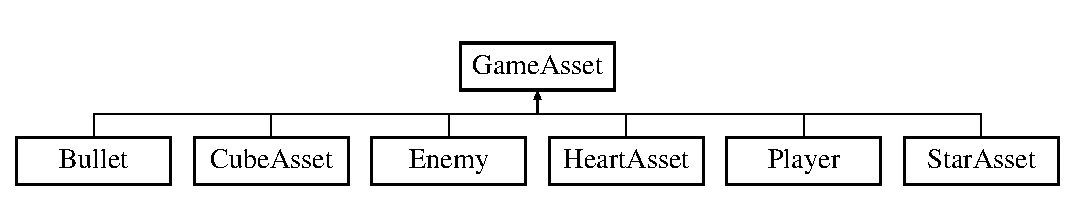
\includegraphics[height=2.000000cm]{classGameAsset}
\end{center}
\end{figure}
\subsection*{Public Member Functions}
\begin{DoxyCompactItemize}
\item 
\hyperlink{classGameAsset_a9c96b0bafa2b6973a2e8c09bf51c52ec}{Game\-Asset} ()
\item 
\hyperlink{classGameAsset_ac6d2340f41dd95e71892327dae4e1585}{Game\-Asset} (const string \&v\-\_\-shader, const string \&f\-\_\-shader)
\item 
virtual \hyperlink{classGameAsset_ace6e367e781c48c6847812778107fcbf}{$\sim$\-Game\-Asset} ()
\item 
bool \hyperlink{classGameAsset_a612793ce2a354d2f8839a779d0ca2227}{collides\-With} (\hyperlink{classGameAsset}{Game\-Asset} \&a)
\item 
virtual void \hyperlink{classGameAsset_a2d7e18a8f1dd8ba89ed1bd14f2affeab}{draw} ()
\item 
virtual void \hyperlink{classGameAsset_a42688ec8f02e201eaaa01e74a112083f}{update} ()=0
\item 
virtual void \hyperlink{classGameAsset_abbea962eaa63a813949b834778b7483e}{clean} ()=0
\item 
virtual bool \hyperlink{classGameAsset_a631982e6d36061c08c7e8981ce0fd308}{dead} ()
\item 
virtual bool \hyperlink{classGameAsset_a3b5885fc74b95141312d6e6d60d0a9d3}{is\-It\-Alive} ()
\end{DoxyCompactItemize}
\subsection*{Public Attributes}
\begin{DoxyCompactItemize}
\item 
shared\-\_\-ptr$<$ \hyperlink{classBoundingBox}{Bounding\-Box} $>$ \hyperlink{classGameAsset_a3444a096fed505b1740bedc95e2cfa6c}{bbox}
\item 
bool \hyperlink{classGameAsset_aebf93ae52dc7fabbb6ec7edaadf915d0}{is\-Alive} = true
\end{DoxyCompactItemize}
\subsection*{Protected Member Functions}
\begin{DoxyCompactItemize}
\item 
int \hyperlink{classGameAsset_aa26d85233ece476d599adf90074e9568}{make\-\_\-resources} ()
\item 
G\-Lchar $\ast$ \hyperlink{classGameAsset_a08c617aafc70dcba441f53260f1bb09f}{shader\-\_\-file\-\_\-contents} (const string \&filename, G\-Lint $\ast$length)
\item 
G\-Luint \hyperlink{classGameAsset_adfe27369433f07092b08f24b0feedfc9}{make\-\_\-buffer} (G\-Lenum target, const void $\ast$buffer\-\_\-data, G\-Lsizei buffer\-\_\-size)
\item 
G\-Luint \hyperlink{classGameAsset_ac728e885b52c93c3e4976a339de54545}{make\-\_\-shader} (G\-Lenum type, const char $\ast$filename)
\item 
G\-Luint \hyperlink{classGameAsset_a9d9574a21cf6b52f7a825879ca50b19d}{make\-\_\-program} (G\-Luint \hyperlink{classGameAsset_aba95de2870f78ac21568bbf9dd7e2b40}{vertex\-\_\-shader}, G\-Luint \hyperlink{classGameAsset_ab62d9e2547537bd89eeae057a402a895}{fragment\-\_\-shader})
\end{DoxyCompactItemize}
\subsection*{Protected Attributes}
\begin{DoxyCompactItemize}
\item 
G\-Luint \hyperlink{classGameAsset_a1a1d227eba2765b025f9f453700c2359}{vertex\-\_\-buffer}
\item 
G\-Luint \hyperlink{classGameAsset_a5e005ff1d4280e73f67446353e78fe43}{element\-\_\-buffer}
\item 
G\-Luint \hyperlink{classGameAsset_aba95de2870f78ac21568bbf9dd7e2b40}{vertex\-\_\-shader}
\item 
G\-Luint \hyperlink{classGameAsset_ab62d9e2547537bd89eeae057a402a895}{fragment\-\_\-shader}
\item 
G\-Luint \hyperlink{classGameAsset_a239f03ead1a34924e76d6f875216404b}{program}
\item 
G\-Lint \hyperlink{classGameAsset_ad8c8198dcc470301e8f5eae8dc8506bb}{position\-\_\-attrib}
\item 
G\-Lint \hyperlink{classGameAsset_a21126e946d621a0e03d61738404b34d2}{tx\-\_\-uniform}
\item 
G\-Lfloat $\ast$ \hyperlink{classGameAsset_ae1d682ecf84d9cd3f91a8c870acf2777}{g\-\_\-vertex\-\_\-buffer\-\_\-data}
\item 
G\-Lushort $\ast$ \hyperlink{classGameAsset_ab859393c9158c8bda39cd100475fee25}{g\-\_\-element\-\_\-buffer\-\_\-data}
\item 
int \hyperlink{classGameAsset_a3e8d7dc58d3d4efafbbce1536b78dbc7}{num\-\_\-vertices}
\item 
int \hyperlink{classGameAsset_aae4d864335c2eca685cc86602881cd18}{num\-\_\-triangles}
\end{DoxyCompactItemize}


\subsection{Detailed Description}


Definition at line 25 of file Game\-Asset.\-h.



\subsection{Constructor \& Destructor Documentation}
\hypertarget{classGameAsset_a9c96b0bafa2b6973a2e8c09bf51c52ec}{\index{Game\-Asset@{Game\-Asset}!Game\-Asset@{Game\-Asset}}
\index{Game\-Asset@{Game\-Asset}!GameAsset@{Game\-Asset}}
\subsubsection[{Game\-Asset}]{\setlength{\rightskip}{0pt plus 5cm}Game\-Asset\-::\-Game\-Asset (
\begin{DoxyParamCaption}
{}
\end{DoxyParamCaption}
)}}\label{classGameAsset_a9c96b0bafa2b6973a2e8c09bf51c52ec}


Definition at line 14 of file Game\-Asset.\-cpp.


\begin{DoxyCode}
14                      \{
15   common\_init();
16   this->v\_shader = \textcolor{stringliteral}{"CubeRacer/shaders/hello-gl.v.glsl"};
17   this->f\_shader = \textcolor{stringliteral}{"CubeRacer/shaders/player-gl.f.glsl"};
18 \}
\end{DoxyCode}
\hypertarget{classGameAsset_ac6d2340f41dd95e71892327dae4e1585}{\index{Game\-Asset@{Game\-Asset}!Game\-Asset@{Game\-Asset}}
\index{Game\-Asset@{Game\-Asset}!GameAsset@{Game\-Asset}}
\subsubsection[{Game\-Asset}]{\setlength{\rightskip}{0pt plus 5cm}Game\-Asset\-::\-Game\-Asset (
\begin{DoxyParamCaption}
\item[{const string \&}]{v\-\_\-shader, }
\item[{const string \&}]{f\-\_\-shader}
\end{DoxyParamCaption}
)}}\label{classGameAsset_ac6d2340f41dd95e71892327dae4e1585}


Definition at line 20 of file Game\-Asset.\-cpp.


\begin{DoxyCode}
20                                                                      \{
21   common\_init();
22   this->v\_shader = v\_shader;
23   this->f\_shader = f\_shader;
24 \}
\end{DoxyCode}
\hypertarget{classGameAsset_ace6e367e781c48c6847812778107fcbf}{\index{Game\-Asset@{Game\-Asset}!$\sim$\-Game\-Asset@{$\sim$\-Game\-Asset}}
\index{$\sim$\-Game\-Asset@{$\sim$\-Game\-Asset}!GameAsset@{Game\-Asset}}
\subsubsection[{$\sim$\-Game\-Asset}]{\setlength{\rightskip}{0pt plus 5cm}Game\-Asset\-::$\sim$\-Game\-Asset (
\begin{DoxyParamCaption}
{}
\end{DoxyParamCaption}
)\hspace{0.3cm}{\ttfamily [virtual]}}}\label{classGameAsset_ace6e367e781c48c6847812778107fcbf}


Definition at line 26 of file Game\-Asset.\-cpp.


\begin{DoxyCode}
26                       \{
27     \textcolor{comment}{// TODO Auto-generated destructor stub}
28 \}
\end{DoxyCode}


\subsection{Member Function Documentation}
\hypertarget{classGameAsset_abbea962eaa63a813949b834778b7483e}{\index{Game\-Asset@{Game\-Asset}!clean@{clean}}
\index{clean@{clean}!GameAsset@{Game\-Asset}}
\subsubsection[{clean}]{\setlength{\rightskip}{0pt plus 5cm}virtual void Game\-Asset\-::clean (
\begin{DoxyParamCaption}
{}
\end{DoxyParamCaption}
)\hspace{0.3cm}{\ttfamily [pure virtual]}}}\label{classGameAsset_abbea962eaa63a813949b834778b7483e}


Implemented in \hyperlink{classPlayer_a883c81df5be3b931ecfa6c8de08acfbd}{Player}, \hyperlink{classEnemy_a12e87c9cb633fed1d846a61cfe7f91c7}{Enemy}, \hyperlink{classHeartAsset_a33b4a41bfc915fc95d23d9b1fbf68dad}{Heart\-Asset}, \hyperlink{classStarAsset_a0e0f4afbd0edd0d10b7e4a2810222c66}{Star\-Asset}, \hyperlink{classBullet_a1a4ffaed3fe46e010bb981ebbbd38ecd}{Bullet}, and \hyperlink{classCubeAsset_af158511433013403bc4fe0c13e8577f3}{Cube\-Asset}.

\hypertarget{classGameAsset_a612793ce2a354d2f8839a779d0ca2227}{\index{Game\-Asset@{Game\-Asset}!collides\-With@{collides\-With}}
\index{collides\-With@{collides\-With}!GameAsset@{Game\-Asset}}
\subsubsection[{collides\-With}]{\setlength{\rightskip}{0pt plus 5cm}bool Game\-Asset\-::collides\-With (
\begin{DoxyParamCaption}
\item[{{\bf Game\-Asset} \&}]{a}
\end{DoxyParamCaption}
)}}\label{classGameAsset_a612793ce2a354d2f8839a779d0ca2227}


Definition at line 30 of file Game\-Asset.\-cpp.


\begin{DoxyCode}
30                                           \{
31   \textcolor{keywordflow}{return} \hyperlink{classGameAsset_a3444a096fed505b1740bedc95e2cfa6c}{bbox}->collidesWith((*a.\hyperlink{classGameAsset_a3444a096fed505b1740bedc95e2cfa6c}{bbox}));
32 \}
\end{DoxyCode}
\hypertarget{classGameAsset_a631982e6d36061c08c7e8981ce0fd308}{\index{Game\-Asset@{Game\-Asset}!dead@{dead}}
\index{dead@{dead}!GameAsset@{Game\-Asset}}
\subsubsection[{dead}]{\setlength{\rightskip}{0pt plus 5cm}virtual bool Game\-Asset\-::dead (
\begin{DoxyParamCaption}
{}
\end{DoxyParamCaption}
)\hspace{0.3cm}{\ttfamily [inline]}, {\ttfamily [virtual]}}}\label{classGameAsset_a631982e6d36061c08c7e8981ce0fd308}


Definition at line 36 of file Game\-Asset.\-h.


\begin{DoxyCode}
36 \{ \hyperlink{classGameAsset_aebf93ae52dc7fabbb6ec7edaadf915d0}{isAlive} = \textcolor{keyword}{false}; \};
\end{DoxyCode}
\hypertarget{classGameAsset_a2d7e18a8f1dd8ba89ed1bd14f2affeab}{\index{Game\-Asset@{Game\-Asset}!draw@{draw}}
\index{draw@{draw}!GameAsset@{Game\-Asset}}
\subsubsection[{draw}]{\setlength{\rightskip}{0pt plus 5cm}void Game\-Asset\-::draw (
\begin{DoxyParamCaption}
{}
\end{DoxyParamCaption}
)\hspace{0.3cm}{\ttfamily [virtual]}}}\label{classGameAsset_a2d7e18a8f1dd8ba89ed1bd14f2affeab}


Reimplemented in \hyperlink{classPlayer_ac18c9d30d2997765321c62030a4b20b7}{Player}, \hyperlink{classEnemy_a7dcf45915f6288ef9264ec60af621b6c}{Enemy}, \hyperlink{classHeartAsset_a12139c94af340272cfcb726a5665bede}{Heart\-Asset}, \hyperlink{classStarAsset_a0ebfee331ac06d5e58ee0226104ac4e2}{Star\-Asset}, \hyperlink{classBullet_a3912974232447f64002fd657340a7b3b}{Bullet}, and \hyperlink{classCubeAsset_ae986d0b82941b268666f697877530ca5}{Cube\-Asset}.



Definition at line 34 of file Game\-Asset.\-cpp.


\begin{DoxyCode}
34                      \{
35   glUseProgram(\hyperlink{classGameAsset_a239f03ead1a34924e76d6f875216404b}{program});
36   
37   \hyperlink{classVectormath_1_1Aos_1_1Vector4}{Vector4} tx = \hyperlink{classCamera_aa84baebe5d771ddfd82a5b55bd3fde39}{Camera::getInstance}().\hyperlink{classCamera_a156b6aba4309cde6f0252ff325663e2f}{getCameraM}() * *(
      \hyperlink{classGameAsset_a3444a096fed505b1740bedc95e2cfa6c}{bbox}->getCentre());
38   \textcolor{keywordtype}{float} tx\_unpacked[] = \{tx.\hyperlink{classVectormath_1_1Aos_1_1Vector4_af067fb75d2fdf3a88189229131f36329}{getX}(), tx.\hyperlink{classVectormath_1_1Aos_1_1Vector4_a895b1271a74265bb853772718aca2b24}{getY}(), tx.\hyperlink{classVectormath_1_1Aos_1_1Vector4_a51336902d57b1c54df19fb708e93b4f2}{getZ}(), tx.\hyperlink{classVectormath_1_1Aos_1_1Vector4_a775bd40a8bd926cd510d39e890c0b686}{getW}()\};
39 
40   \textcolor{comment}{//  std::cout << "tx.x " << tx.getX() << "\(\backslash\)ttx.y " << tx.getY() << "\(\backslash\)t tx.z " << tx.getZ() << std::endl;}
41   
42   glUniform4fv(\hyperlink{classGameAsset_a21126e946d621a0e03d61738404b34d2}{tx\_uniform}, 1, tx\_unpacked);
43 
44   glBindBuffer(GL\_ARRAY\_BUFFER, \hyperlink{classGameAsset_a1a1d227eba2765b025f9f453700c2359}{vertex\_buffer});
45   glVertexAttribPointer(
46             \hyperlink{classGameAsset_ad8c8198dcc470301e8f5eae8dc8506bb}{position\_attrib},                  \textcolor{comment}{/* attribute */}
47             3,                                \textcolor{comment}{/* size */}
48             GL\_FLOAT,                         \textcolor{comment}{/* type */}
49             GL\_FALSE,                         \textcolor{comment}{/* normalized? */}
50             0,                                \textcolor{comment}{/* stride */}
51             (\textcolor{keywordtype}{void}*)0                          \textcolor{comment}{/* array buffer offset */}
52             );
53   glEnableVertexAttribArray(\hyperlink{classGameAsset_ad8c8198dcc470301e8f5eae8dc8506bb}{position\_attrib});
54   
55   glBindBuffer(GL\_ELEMENT\_ARRAY\_BUFFER, \hyperlink{classGameAsset_a5e005ff1d4280e73f67446353e78fe43}{element\_buffer});
56   glDrawElements(
57          GL\_TRIANGLES,
58          3 * this->\hyperlink{classGameAsset_aae4d864335c2eca685cc86602881cd18}{num\_triangles},
59          GL\_UNSIGNED\_SHORT,
60          (GLvoid*) 0
61          );
62   
63   glDisableVertexAttribArray(\hyperlink{classGameAsset_ad8c8198dcc470301e8f5eae8dc8506bb}{position\_attrib});
64 \}
\end{DoxyCode}
\hypertarget{classGameAsset_a3b5885fc74b95141312d6e6d60d0a9d3}{\index{Game\-Asset@{Game\-Asset}!is\-It\-Alive@{is\-It\-Alive}}
\index{is\-It\-Alive@{is\-It\-Alive}!GameAsset@{Game\-Asset}}
\subsubsection[{is\-It\-Alive}]{\setlength{\rightskip}{0pt plus 5cm}virtual bool Game\-Asset\-::is\-It\-Alive (
\begin{DoxyParamCaption}
{}
\end{DoxyParamCaption}
)\hspace{0.3cm}{\ttfamily [inline]}, {\ttfamily [virtual]}}}\label{classGameAsset_a3b5885fc74b95141312d6e6d60d0a9d3}


Definition at line 37 of file Game\-Asset.\-h.


\begin{DoxyCode}
37 \{ \textcolor{keywordflow}{return} \hyperlink{classGameAsset_aebf93ae52dc7fabbb6ec7edaadf915d0}{isAlive}; \};
\end{DoxyCode}
\hypertarget{classGameAsset_adfe27369433f07092b08f24b0feedfc9}{\index{Game\-Asset@{Game\-Asset}!make\-\_\-buffer@{make\-\_\-buffer}}
\index{make\-\_\-buffer@{make\-\_\-buffer}!GameAsset@{Game\-Asset}}
\subsubsection[{make\-\_\-buffer}]{\setlength{\rightskip}{0pt plus 5cm}G\-Luint Game\-Asset\-::make\-\_\-buffer (
\begin{DoxyParamCaption}
\item[{G\-Lenum}]{target, }
\item[{const void $\ast$}]{buffer\-\_\-data, }
\item[{G\-Lsizei}]{buffer\-\_\-size}
\end{DoxyParamCaption}
)\hspace{0.3cm}{\ttfamily [protected]}}}\label{classGameAsset_adfe27369433f07092b08f24b0feedfc9}


Definition at line 89 of file Game\-Asset.\-cpp.


\begin{DoxyCode}
93   \{
94     GLuint buffer;
95     glGenBuffers(1, &buffer);
96     glBindBuffer(target, buffer);
97     glBufferData(target, buffer\_size, buffer\_data, GL\_STATIC\_DRAW);
98     \textcolor{keywordflow}{return} buffer;
99 \}
\end{DoxyCode}
\hypertarget{classGameAsset_a9d9574a21cf6b52f7a825879ca50b19d}{\index{Game\-Asset@{Game\-Asset}!make\-\_\-program@{make\-\_\-program}}
\index{make\-\_\-program@{make\-\_\-program}!GameAsset@{Game\-Asset}}
\subsubsection[{make\-\_\-program}]{\setlength{\rightskip}{0pt plus 5cm}G\-Luint Game\-Asset\-::make\-\_\-program (
\begin{DoxyParamCaption}
\item[{G\-Luint}]{vertex\-\_\-shader, }
\item[{G\-Luint}]{fragment\-\_\-shader}
\end{DoxyParamCaption}
)\hspace{0.3cm}{\ttfamily [protected]}}}\label{classGameAsset_a9d9574a21cf6b52f7a825879ca50b19d}


Definition at line 125 of file Game\-Asset.\-cpp.


\begin{DoxyCode}
126 \{
127     GLint program\_ok;
128 
129     GLuint \hyperlink{classGameAsset_a239f03ead1a34924e76d6f875216404b}{program} = glCreateProgram();
130 
131     glAttachShader(program, \hyperlink{classGameAsset_aba95de2870f78ac21568bbf9dd7e2b40}{vertex\_shader});
132     glAttachShader(program, \hyperlink{classGameAsset_ab62d9e2547537bd89eeae057a402a895}{fragment\_shader});
133     glLinkProgram(program);
134 
135     glGetProgramiv(program, GL\_LINK\_STATUS, &program\_ok);
136     \textcolor{keywordflow}{if} (!program\_ok) \{
137         cerr<< \textcolor{stringliteral}{"Failed to link shader program:"} << endl;
138         glDeleteProgram(program);
139         \textcolor{keywordflow}{return} 0;
140     \}
141     \textcolor{keywordflow}{return} \hyperlink{classGameAsset_a239f03ead1a34924e76d6f875216404b}{program};
142 \}
\end{DoxyCode}
\hypertarget{classGameAsset_aa26d85233ece476d599adf90074e9568}{\index{Game\-Asset@{Game\-Asset}!make\-\_\-resources@{make\-\_\-resources}}
\index{make\-\_\-resources@{make\-\_\-resources}!GameAsset@{Game\-Asset}}
\subsubsection[{make\-\_\-resources}]{\setlength{\rightskip}{0pt plus 5cm}int Game\-Asset\-::make\-\_\-resources (
\begin{DoxyParamCaption}
\item[{void}]{}
\end{DoxyParamCaption}
)\hspace{0.3cm}{\ttfamily [protected]}}}\label{classGameAsset_aa26d85233ece476d599adf90074e9568}


Definition at line 147 of file Game\-Asset.\-cpp.


\begin{DoxyCode}
148 \{
149     \hyperlink{classGameAsset_a1a1d227eba2765b025f9f453700c2359}{vertex\_buffer} = \hyperlink{classGameAsset_adfe27369433f07092b08f24b0feedfc9}{make\_buffer}(
150         GL\_ARRAY\_BUFFER,
151         \hyperlink{classGameAsset_ae1d682ecf84d9cd3f91a8c870acf2777}{g\_vertex\_buffer\_data},
152         3 * \textcolor{keyword}{sizeof}(GLfloat) * this->\hyperlink{classGameAsset_a3e8d7dc58d3d4efafbbce1536b78dbc7}{num\_vertices}
153     );
154     \hyperlink{classGameAsset_a5e005ff1d4280e73f67446353e78fe43}{element\_buffer} = \hyperlink{classGameAsset_adfe27369433f07092b08f24b0feedfc9}{make\_buffer}(
155         GL\_ELEMENT\_ARRAY\_BUFFER,
156         \hyperlink{classGameAsset_ab859393c9158c8bda39cd100475fee25}{g\_element\_buffer\_data},
157         3 *  \textcolor{keyword}{sizeof}(GLushort) * this->\hyperlink{classGameAsset_aae4d864335c2eca685cc86602881cd18}{num\_triangles}
158     );
159 
160     \hyperlink{classGameAsset_aba95de2870f78ac21568bbf9dd7e2b40}{vertex\_shader} = \hyperlink{classGameAsset_ac728e885b52c93c3e4976a339de54545}{make\_shader}(
161         GL\_VERTEX\_SHADER,
162         this->v\_shader.c\_str()
163     );
164     \textcolor{keywordflow}{if} (\hyperlink{classGameAsset_aba95de2870f78ac21568bbf9dd7e2b40}{vertex\_shader} == 0)
165         \textcolor{keywordflow}{return} 0;
166 
167     \hyperlink{classGameAsset_ab62d9e2547537bd89eeae057a402a895}{fragment\_shader} = \hyperlink{classGameAsset_ac728e885b52c93c3e4976a339de54545}{make\_shader}(
168         GL\_FRAGMENT\_SHADER,
169         this->f\_shader.c\_str()
170     );
171     \textcolor{keywordflow}{if} (\hyperlink{classGameAsset_ab62d9e2547537bd89eeae057a402a895}{fragment\_shader} == 0)
172         \textcolor{keywordflow}{return} 0;
173     
174     \hyperlink{classGameAsset_a239f03ead1a34924e76d6f875216404b}{program} = \hyperlink{classGameAsset_a9d9574a21cf6b52f7a825879ca50b19d}{make\_program}(\hyperlink{classGameAsset_aba95de2870f78ac21568bbf9dd7e2b40}{vertex\_shader}, 
      \hyperlink{classGameAsset_ab62d9e2547537bd89eeae057a402a895}{fragment\_shader});
175     \textcolor{keywordflow}{if} (\hyperlink{classGameAsset_a239f03ead1a34924e76d6f875216404b}{program} == 0)
176         \textcolor{keywordflow}{return} 0;
177 
178     \hyperlink{classGameAsset_ad8c8198dcc470301e8f5eae8dc8506bb}{position\_attrib} = glGetAttribLocation(\hyperlink{classGameAsset_a239f03ead1a34924e76d6f875216404b}{program}, \textcolor{stringliteral}{"position"});
179     \hyperlink{classGameAsset_a21126e946d621a0e03d61738404b34d2}{tx\_uniform} = glGetUniformLocation(\hyperlink{classGameAsset_a239f03ead1a34924e76d6f875216404b}{program}, \textcolor{stringliteral}{"tx"});
180 
181     \textcolor{keywordflow}{return} 1;
182 \}
\end{DoxyCode}
\hypertarget{classGameAsset_ac728e885b52c93c3e4976a339de54545}{\index{Game\-Asset@{Game\-Asset}!make\-\_\-shader@{make\-\_\-shader}}
\index{make\-\_\-shader@{make\-\_\-shader}!GameAsset@{Game\-Asset}}
\subsubsection[{make\-\_\-shader}]{\setlength{\rightskip}{0pt plus 5cm}G\-Luint Game\-Asset\-::make\-\_\-shader (
\begin{DoxyParamCaption}
\item[{G\-Lenum}]{type, }
\item[{const char $\ast$}]{filename}
\end{DoxyParamCaption}
)\hspace{0.3cm}{\ttfamily [protected]}}}\label{classGameAsset_ac728e885b52c93c3e4976a339de54545}


Definition at line 101 of file Game\-Asset.\-cpp.


\begin{DoxyCode}
102 \{
103     GLint \hyperlink{namespaceVectormath_1_1Aos_aa7db613f8732057fec0b26f26aefaff4}{length};
104     GLchar *source = \hyperlink{classGameAsset_a08c617aafc70dcba441f53260f1bb09f}{shader\_file\_contents}(filename, &length);
105     GLuint shader;
106     GLint shader\_ok;
107 
108     \textcolor{keywordflow}{if} (!source)
109         \textcolor{keywordflow}{return} 0;
110 
111     shader = glCreateShader(type);
112     glShaderSource(shader, 1, (\textcolor{keyword}{const} GLchar**)&source, &length);
113     \textcolor{keyword}{delete}(source);
114     glCompileShader(shader);
115 
116     glGetShaderiv(shader, GL\_COMPILE\_STATUS, &shader\_ok);
117     \textcolor{keywordflow}{if} (!shader\_ok) \{
118         cerr << \textcolor{stringliteral}{"Failed to compile "} << filename << \textcolor{stringliteral}{" with error code "} << shader\_ok << endl;
119         glDeleteShader(shader);
120         \textcolor{keywordflow}{return} 0;
121     \}
122     \textcolor{keywordflow}{return} shader;
123 \}
\end{DoxyCode}
\hypertarget{classGameAsset_a08c617aafc70dcba441f53260f1bb09f}{\index{Game\-Asset@{Game\-Asset}!shader\-\_\-file\-\_\-contents@{shader\-\_\-file\-\_\-contents}}
\index{shader\-\_\-file\-\_\-contents@{shader\-\_\-file\-\_\-contents}!GameAsset@{Game\-Asset}}
\subsubsection[{shader\-\_\-file\-\_\-contents}]{\setlength{\rightskip}{0pt plus 5cm}G\-Lchar $\ast$ Game\-Asset\-::shader\-\_\-file\-\_\-contents (
\begin{DoxyParamCaption}
\item[{const string \&}]{filename, }
\item[{G\-Lint $\ast$}]{length}
\end{DoxyParamCaption}
)\hspace{0.3cm}{\ttfamily [protected]}}}\label{classGameAsset_a08c617aafc70dcba441f53260f1bb09f}


Definition at line 69 of file Game\-Asset.\-cpp.


\begin{DoxyCode}
70 \{
71   ifstream input\_file;
72   input\_file.open(filename.c\_str(), ios::in);
73 
74   input\_file.seekg(0, ios::end);  \textcolor{comment}{// go to the end of the file}
75   *\hyperlink{namespaceVectormath_1_1Aos_aa7db613f8732057fec0b26f26aefaff4}{length} = input\_file.tellg();  \textcolor{comment}{// get length of the file}
76   input\_file.seekg(0, ios::beg);  \textcolor{comment}{// go to beginning of the file}
77 
78   GLchar * buffer = \textcolor{keyword}{new} GLchar[(*length)+1];
79   input\_file.read(buffer, *\hyperlink{namespaceVectormath_1_1Aos_aa7db613f8732057fec0b26f26aefaff4}{length});
80   buffer[(*length)+1]=\textcolor{charliteral}{'\(\backslash\)0'};  \textcolor{comment}{// Ensure null terminated}
81 
82   input\_file.close();
83   \textcolor{keywordflow}{return} buffer;
84 \}
\end{DoxyCode}
\hypertarget{classGameAsset_a42688ec8f02e201eaaa01e74a112083f}{\index{Game\-Asset@{Game\-Asset}!update@{update}}
\index{update@{update}!GameAsset@{Game\-Asset}}
\subsubsection[{update}]{\setlength{\rightskip}{0pt plus 5cm}virtual void Game\-Asset\-::update (
\begin{DoxyParamCaption}
{}
\end{DoxyParamCaption}
)\hspace{0.3cm}{\ttfamily [pure virtual]}}}\label{classGameAsset_a42688ec8f02e201eaaa01e74a112083f}


Implemented in \hyperlink{classPlayer_a82c3476f3e65a4e2ac6bcd040771bdd4}{Player}, \hyperlink{classEnemy_ad55ee71b5a8c23fbd00b3c368b90cc64}{Enemy}, \hyperlink{classHeartAsset_aa4fb245ae438223980f781cb070e0050}{Heart\-Asset}, \hyperlink{classStarAsset_a21f6e7f632408f34209db35d41f41877}{Star\-Asset}, \hyperlink{classBullet_a32f4a0611fe2dd245fee955d14ca1f68}{Bullet}, and \hyperlink{classCubeAsset_a45f15f556999ddb0789eaf01fb0df45d}{Cube\-Asset}.



\subsection{Member Data Documentation}
\hypertarget{classGameAsset_a3444a096fed505b1740bedc95e2cfa6c}{\index{Game\-Asset@{Game\-Asset}!bbox@{bbox}}
\index{bbox@{bbox}!GameAsset@{Game\-Asset}}
\subsubsection[{bbox}]{\setlength{\rightskip}{0pt plus 5cm}shared\-\_\-ptr$<${\bf Bounding\-Box}$>$ Game\-Asset\-::bbox}}\label{classGameAsset_a3444a096fed505b1740bedc95e2cfa6c}


Definition at line 37 of file Game\-Asset.\-h.

\hypertarget{classGameAsset_a5e005ff1d4280e73f67446353e78fe43}{\index{Game\-Asset@{Game\-Asset}!element\-\_\-buffer@{element\-\_\-buffer}}
\index{element\-\_\-buffer@{element\-\_\-buffer}!GameAsset@{Game\-Asset}}
\subsubsection[{element\-\_\-buffer}]{\setlength{\rightskip}{0pt plus 5cm}G\-Luint Game\-Asset\-::element\-\_\-buffer\hspace{0.3cm}{\ttfamily [protected]}}}\label{classGameAsset_a5e005ff1d4280e73f67446353e78fe43}


Definition at line 51 of file Game\-Asset.\-h.

\hypertarget{classGameAsset_ab62d9e2547537bd89eeae057a402a895}{\index{Game\-Asset@{Game\-Asset}!fragment\-\_\-shader@{fragment\-\_\-shader}}
\index{fragment\-\_\-shader@{fragment\-\_\-shader}!GameAsset@{Game\-Asset}}
\subsubsection[{fragment\-\_\-shader}]{\setlength{\rightskip}{0pt plus 5cm}G\-Luint Game\-Asset\-::fragment\-\_\-shader\hspace{0.3cm}{\ttfamily [protected]}}}\label{classGameAsset_ab62d9e2547537bd89eeae057a402a895}


Definition at line 52 of file Game\-Asset.\-h.

\hypertarget{classGameAsset_ab859393c9158c8bda39cd100475fee25}{\index{Game\-Asset@{Game\-Asset}!g\-\_\-element\-\_\-buffer\-\_\-data@{g\-\_\-element\-\_\-buffer\-\_\-data}}
\index{g\-\_\-element\-\_\-buffer\-\_\-data@{g\-\_\-element\-\_\-buffer\-\_\-data}!GameAsset@{Game\-Asset}}
\subsubsection[{g\-\_\-element\-\_\-buffer\-\_\-data}]{\setlength{\rightskip}{0pt plus 5cm}G\-Lushort$\ast$ Game\-Asset\-::g\-\_\-element\-\_\-buffer\-\_\-data\hspace{0.3cm}{\ttfamily [protected]}}}\label{classGameAsset_ab859393c9158c8bda39cd100475fee25}


Definition at line 57 of file Game\-Asset.\-h.

\hypertarget{classGameAsset_ae1d682ecf84d9cd3f91a8c870acf2777}{\index{Game\-Asset@{Game\-Asset}!g\-\_\-vertex\-\_\-buffer\-\_\-data@{g\-\_\-vertex\-\_\-buffer\-\_\-data}}
\index{g\-\_\-vertex\-\_\-buffer\-\_\-data@{g\-\_\-vertex\-\_\-buffer\-\_\-data}!GameAsset@{Game\-Asset}}
\subsubsection[{g\-\_\-vertex\-\_\-buffer\-\_\-data}]{\setlength{\rightskip}{0pt plus 5cm}G\-Lfloat$\ast$ Game\-Asset\-::g\-\_\-vertex\-\_\-buffer\-\_\-data\hspace{0.3cm}{\ttfamily [protected]}}}\label{classGameAsset_ae1d682ecf84d9cd3f91a8c870acf2777}


Definition at line 56 of file Game\-Asset.\-h.

\hypertarget{classGameAsset_aebf93ae52dc7fabbb6ec7edaadf915d0}{\index{Game\-Asset@{Game\-Asset}!is\-Alive@{is\-Alive}}
\index{is\-Alive@{is\-Alive}!GameAsset@{Game\-Asset}}
\subsubsection[{is\-Alive}]{\setlength{\rightskip}{0pt plus 5cm}bool Game\-Asset\-::is\-Alive = true}}\label{classGameAsset_aebf93ae52dc7fabbb6ec7edaadf915d0}


Definition at line 40 of file Game\-Asset.\-h.

\hypertarget{classGameAsset_aae4d864335c2eca685cc86602881cd18}{\index{Game\-Asset@{Game\-Asset}!num\-\_\-triangles@{num\-\_\-triangles}}
\index{num\-\_\-triangles@{num\-\_\-triangles}!GameAsset@{Game\-Asset}}
\subsubsection[{num\-\_\-triangles}]{\setlength{\rightskip}{0pt plus 5cm}int Game\-Asset\-::num\-\_\-triangles\hspace{0.3cm}{\ttfamily [protected]}}}\label{classGameAsset_aae4d864335c2eca685cc86602881cd18}


Definition at line 61 of file Game\-Asset.\-h.

\hypertarget{classGameAsset_a3e8d7dc58d3d4efafbbce1536b78dbc7}{\index{Game\-Asset@{Game\-Asset}!num\-\_\-vertices@{num\-\_\-vertices}}
\index{num\-\_\-vertices@{num\-\_\-vertices}!GameAsset@{Game\-Asset}}
\subsubsection[{num\-\_\-vertices}]{\setlength{\rightskip}{0pt plus 5cm}int Game\-Asset\-::num\-\_\-vertices\hspace{0.3cm}{\ttfamily [protected]}}}\label{classGameAsset_a3e8d7dc58d3d4efafbbce1536b78dbc7}


Definition at line 60 of file Game\-Asset.\-h.

\hypertarget{classGameAsset_ad8c8198dcc470301e8f5eae8dc8506bb}{\index{Game\-Asset@{Game\-Asset}!position\-\_\-attrib@{position\-\_\-attrib}}
\index{position\-\_\-attrib@{position\-\_\-attrib}!GameAsset@{Game\-Asset}}
\subsubsection[{position\-\_\-attrib}]{\setlength{\rightskip}{0pt plus 5cm}G\-Lint Game\-Asset\-::position\-\_\-attrib\hspace{0.3cm}{\ttfamily [protected]}}}\label{classGameAsset_ad8c8198dcc470301e8f5eae8dc8506bb}


Definition at line 53 of file Game\-Asset.\-h.

\hypertarget{classGameAsset_a239f03ead1a34924e76d6f875216404b}{\index{Game\-Asset@{Game\-Asset}!program@{program}}
\index{program@{program}!GameAsset@{Game\-Asset}}
\subsubsection[{program}]{\setlength{\rightskip}{0pt plus 5cm}G\-Luint Game\-Asset\-::program\hspace{0.3cm}{\ttfamily [protected]}}}\label{classGameAsset_a239f03ead1a34924e76d6f875216404b}


Definition at line 52 of file Game\-Asset.\-h.

\hypertarget{classGameAsset_a21126e946d621a0e03d61738404b34d2}{\index{Game\-Asset@{Game\-Asset}!tx\-\_\-uniform@{tx\-\_\-uniform}}
\index{tx\-\_\-uniform@{tx\-\_\-uniform}!GameAsset@{Game\-Asset}}
\subsubsection[{tx\-\_\-uniform}]{\setlength{\rightskip}{0pt plus 5cm}G\-Lint Game\-Asset\-::tx\-\_\-uniform\hspace{0.3cm}{\ttfamily [protected]}}}\label{classGameAsset_a21126e946d621a0e03d61738404b34d2}


Definition at line 54 of file Game\-Asset.\-h.

\hypertarget{classGameAsset_a1a1d227eba2765b025f9f453700c2359}{\index{Game\-Asset@{Game\-Asset}!vertex\-\_\-buffer@{vertex\-\_\-buffer}}
\index{vertex\-\_\-buffer@{vertex\-\_\-buffer}!GameAsset@{Game\-Asset}}
\subsubsection[{vertex\-\_\-buffer}]{\setlength{\rightskip}{0pt plus 5cm}G\-Luint Game\-Asset\-::vertex\-\_\-buffer\hspace{0.3cm}{\ttfamily [protected]}}}\label{classGameAsset_a1a1d227eba2765b025f9f453700c2359}


Definition at line 51 of file Game\-Asset.\-h.

\hypertarget{classGameAsset_aba95de2870f78ac21568bbf9dd7e2b40}{\index{Game\-Asset@{Game\-Asset}!vertex\-\_\-shader@{vertex\-\_\-shader}}
\index{vertex\-\_\-shader@{vertex\-\_\-shader}!GameAsset@{Game\-Asset}}
\subsubsection[{vertex\-\_\-shader}]{\setlength{\rightskip}{0pt plus 5cm}G\-Luint Game\-Asset\-::vertex\-\_\-shader\hspace{0.3cm}{\ttfamily [protected]}}}\label{classGameAsset_aba95de2870f78ac21568bbf9dd7e2b40}


Definition at line 52 of file Game\-Asset.\-h.



The documentation for this class was generated from the following files\-:\begin{DoxyCompactItemize}
\item 
/home/sam/\-Cube\-Racer/src/\hyperlink{GameAsset_8h}{Game\-Asset.\-h}\item 
/home/sam/\-Cube\-Racer/src/\hyperlink{GameAsset_8cpp}{Game\-Asset.\-cpp}\end{DoxyCompactItemize}

\hypertarget{classHeartAsset}{\section{Heart\-Asset Class Reference}
\label{classHeartAsset}\index{Heart\-Asset@{Heart\-Asset}}
}


{\ttfamily \#include $<$Heart\-Asset.\-h$>$}

Inheritance diagram for Heart\-Asset\-:\begin{figure}[H]
\begin{center}
\leavevmode
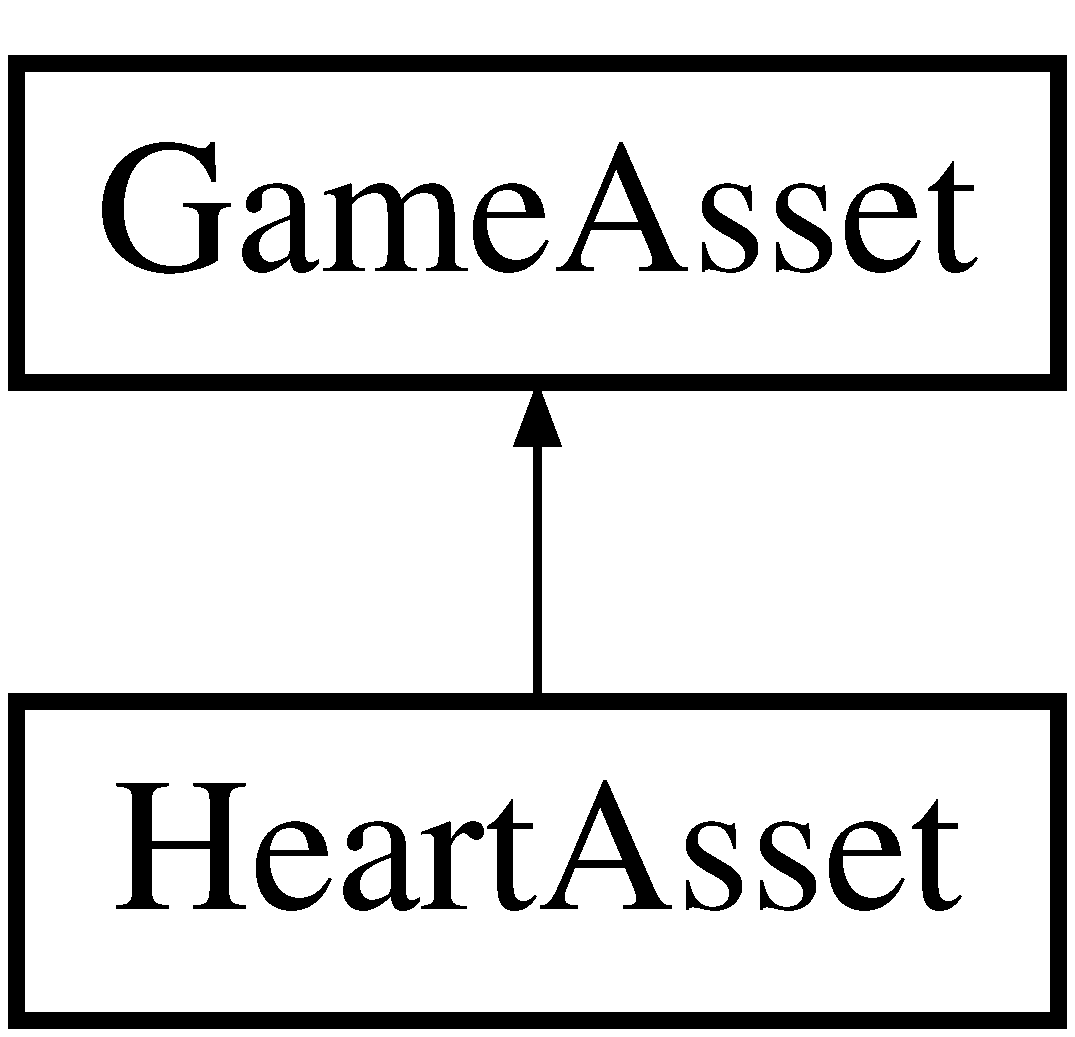
\includegraphics[height=2.000000cm]{classHeartAsset}
\end{center}
\end{figure}
\subsection*{Public Types}
\begin{DoxyCompactItemize}
\item 
enum \hyperlink{classHeartAsset_ab2382a6a68d870ea588f3e993a1451d0}{vertices} \{ \\*
\hyperlink{classHeartAsset_ab2382a6a68d870ea588f3e993a1451d0a3b7c6d42e96cb2f900f179d223236f11}{F0}, 
\hyperlink{classHeartAsset_ab2382a6a68d870ea588f3e993a1451d0af6d5902a14c48e5f35f74c16afafbe9a}{F1}, 
\hyperlink{classHeartAsset_ab2382a6a68d870ea588f3e993a1451d0a9da21cb8da0427c073dc2260b549e761}{F2}, 
\hyperlink{classHeartAsset_ab2382a6a68d870ea588f3e993a1451d0a0280f1f7097bf67d876440c3cf2e361c}{F3}, 
\\*
\hyperlink{classHeartAsset_ab2382a6a68d870ea588f3e993a1451d0a37d27782c67bdb394c66fde29473ddf3}{F4}, 
\hyperlink{classHeartAsset_ab2382a6a68d870ea588f3e993a1451d0ac5e53a8bb99468ed9401d0067cf96eb8}{F5}
 \}
\end{DoxyCompactItemize}
\subsection*{Public Member Functions}
\begin{DoxyCompactItemize}
\item 
\hyperlink{classHeartAsset_a68370016b5184e3e541070eac1ebaed4}{Heart\-Asset} ()
\item 
\hyperlink{classHeartAsset_ac9be59ddbf1799b9523b94b224c2ebdd}{Heart\-Asset} (float x, float y, float z)
\item 
\hyperlink{classHeartAsset_a188438e39a1e5242ab9da9b3574cf1e5}{$\sim$\-Heart\-Asset} ()
\item 
bool \hyperlink{classHeartAsset_aeeea2e4cebcb2e238544607ab8fcb7b7}{collides\-With} (\hyperlink{classPlayer}{Player} \&a)
\item 
virtual void \hyperlink{classHeartAsset_aa4fb245ae438223980f781cb070e0050}{update} ()
\item 
virtual void \hyperlink{classHeartAsset_a12139c94af340272cfcb726a5665bede}{draw} ()
\item 
virtual void \hyperlink{classHeartAsset_a33b4a41bfc915fc95d23d9b1fbf68dad}{clean} ()
\end{DoxyCompactItemize}
\subsection*{Additional Inherited Members}


\subsection{Detailed Description}


Definition at line 7 of file Heart\-Asset.\-h.



\subsection{Member Enumeration Documentation}
\hypertarget{classHeartAsset_ab2382a6a68d870ea588f3e993a1451d0}{\index{Heart\-Asset@{Heart\-Asset}!vertices@{vertices}}
\index{vertices@{vertices}!HeartAsset@{Heart\-Asset}}
\subsubsection[{vertices}]{\setlength{\rightskip}{0pt plus 5cm}enum {\bf Heart\-Asset\-::vertices}}}\label{classHeartAsset_ab2382a6a68d870ea588f3e993a1451d0}
\begin{Desc}
\item[Enumerator]\par
\begin{description}
\index{F0@{F0}!Heart\-Asset@{Heart\-Asset}}\index{Heart\-Asset@{Heart\-Asset}!F0@{F0}}\item[{\em 
\hypertarget{classHeartAsset_ab2382a6a68d870ea588f3e993a1451d0a3b7c6d42e96cb2f900f179d223236f11}{F0}\label{classHeartAsset_ab2382a6a68d870ea588f3e993a1451d0a3b7c6d42e96cb2f900f179d223236f11}
}]\index{F1@{F1}!Heart\-Asset@{Heart\-Asset}}\index{Heart\-Asset@{Heart\-Asset}!F1@{F1}}\item[{\em 
\hypertarget{classHeartAsset_ab2382a6a68d870ea588f3e993a1451d0af6d5902a14c48e5f35f74c16afafbe9a}{F1}\label{classHeartAsset_ab2382a6a68d870ea588f3e993a1451d0af6d5902a14c48e5f35f74c16afafbe9a}
}]\index{F2@{F2}!Heart\-Asset@{Heart\-Asset}}\index{Heart\-Asset@{Heart\-Asset}!F2@{F2}}\item[{\em 
\hypertarget{classHeartAsset_ab2382a6a68d870ea588f3e993a1451d0a9da21cb8da0427c073dc2260b549e761}{F2}\label{classHeartAsset_ab2382a6a68d870ea588f3e993a1451d0a9da21cb8da0427c073dc2260b549e761}
}]\index{F3@{F3}!Heart\-Asset@{Heart\-Asset}}\index{Heart\-Asset@{Heart\-Asset}!F3@{F3}}\item[{\em 
\hypertarget{classHeartAsset_ab2382a6a68d870ea588f3e993a1451d0a0280f1f7097bf67d876440c3cf2e361c}{F3}\label{classHeartAsset_ab2382a6a68d870ea588f3e993a1451d0a0280f1f7097bf67d876440c3cf2e361c}
}]\index{F4@{F4}!Heart\-Asset@{Heart\-Asset}}\index{Heart\-Asset@{Heart\-Asset}!F4@{F4}}\item[{\em 
\hypertarget{classHeartAsset_ab2382a6a68d870ea588f3e993a1451d0a37d27782c67bdb394c66fde29473ddf3}{F4}\label{classHeartAsset_ab2382a6a68d870ea588f3e993a1451d0a37d27782c67bdb394c66fde29473ddf3}
}]\index{F5@{F5}!Heart\-Asset@{Heart\-Asset}}\index{Heart\-Asset@{Heart\-Asset}!F5@{F5}}\item[{\em 
\hypertarget{classHeartAsset_ab2382a6a68d870ea588f3e993a1451d0ac5e53a8bb99468ed9401d0067cf96eb8}{F5}\label{classHeartAsset_ab2382a6a68d870ea588f3e993a1451d0ac5e53a8bb99468ed9401d0067cf96eb8}
}]\end{description}
\end{Desc}


Definition at line 19 of file Heart\-Asset.\-h.


\begin{DoxyCode}
19                 \{
20       \hyperlink{classHeartAsset_ab2382a6a68d870ea588f3e993a1451d0a3b7c6d42e96cb2f900f179d223236f11}{F0}, \hyperlink{classHeartAsset_ab2382a6a68d870ea588f3e993a1451d0af6d5902a14c48e5f35f74c16afafbe9a}{F1}, \hyperlink{classHeartAsset_ab2382a6a68d870ea588f3e993a1451d0a9da21cb8da0427c073dc2260b549e761}{F2}, \hyperlink{classHeartAsset_ab2382a6a68d870ea588f3e993a1451d0a0280f1f7097bf67d876440c3cf2e361c}{F3}, \hyperlink{classHeartAsset_ab2382a6a68d870ea588f3e993a1451d0a37d27782c67bdb394c66fde29473ddf3}{F4}, \hyperlink{classHeartAsset_ab2382a6a68d870ea588f3e993a1451d0ac5e53a8bb99468ed9401d0067cf96eb8}{F5},
21   \};
\end{DoxyCode}


\subsection{Constructor \& Destructor Documentation}
\hypertarget{classHeartAsset_a68370016b5184e3e541070eac1ebaed4}{\index{Heart\-Asset@{Heart\-Asset}!Heart\-Asset@{Heart\-Asset}}
\index{Heart\-Asset@{Heart\-Asset}!HeartAsset@{Heart\-Asset}}
\subsubsection[{Heart\-Asset}]{\setlength{\rightskip}{0pt plus 5cm}Heart\-Asset\-::\-Heart\-Asset (
\begin{DoxyParamCaption}
{}
\end{DoxyParamCaption}
)}}\label{classHeartAsset_a68370016b5184e3e541070eac1ebaed4}


Definition at line 3 of file Heart\-Asset.\-cpp.


\begin{DoxyCode}
4   : \hyperlink{classGameAsset_a9c96b0bafa2b6973a2e8c09bf51c52ec}{GameAsset}(
5           \textcolor{keywordtype}{string}(\textcolor{stringliteral}{"CubeRacer/shaders/hello-gl.v.glsl"})
6           , \textcolor{keywordtype}{string}(\textcolor{stringliteral}{"CubeRacer/shaders/heartAsset.f.glsl"})
7           )
8 \{
9   \hyperlink{classHeartAsset_a68370016b5184e3e541070eac1ebaed4}{HeartAsset}(0, 0, 0);
10 \}
\end{DoxyCode}
\hypertarget{classHeartAsset_ac9be59ddbf1799b9523b94b224c2ebdd}{\index{Heart\-Asset@{Heart\-Asset}!Heart\-Asset@{Heart\-Asset}}
\index{Heart\-Asset@{Heart\-Asset}!HeartAsset@{Heart\-Asset}}
\subsubsection[{Heart\-Asset}]{\setlength{\rightskip}{0pt plus 5cm}Heart\-Asset\-::\-Heart\-Asset (
\begin{DoxyParamCaption}
\item[{float}]{x, }
\item[{float}]{y, }
\item[{float}]{z}
\end{DoxyParamCaption}
)}}\label{classHeartAsset_ac9be59ddbf1799b9523b94b224c2ebdd}


Definition at line 12 of file Heart\-Asset.\-cpp.


\begin{DoxyCode}
13   : \hyperlink{classGameAsset_a9c96b0bafa2b6973a2e8c09bf51c52ec}{GameAsset}(
14       \textcolor{keywordtype}{string}(\textcolor{stringliteral}{"CubeRacer/shaders/hello-gl.v.glsl"}), 
15       \textcolor{keywordtype}{string}(\textcolor{stringliteral}{"CubeRacer/shaders/heartAsset-gl.f.glsl"})
16 )\{
17 
18   \textcolor{comment}{// A default "unit" Heart}
19   \hyperlink{classGameAsset_a3e8d7dc58d3d4efafbbce1536b78dbc7}{num\_vertices} = 6;
20   \hyperlink{classGameAsset_aae4d864335c2eca685cc86602881cd18}{num\_triangles} = 4;
21   \hyperlink{classGameAsset_ae1d682ecf84d9cd3f91a8c870acf2777}{g\_vertex\_buffer\_data} = \textcolor{keyword}{new} GLfloat[\hyperlink{classGameAsset_a3e8d7dc58d3d4efafbbce1536b78dbc7}{num\_vertices} * 3]\{
22 
23   \textcolor{comment}{//     x      y     z    
       //http://www.google.co.uk/imgres?imgurl=&imgrefurl=http%3A%2F%2Fcollectionphotos
      .com%2Fnice-love-hearts%2F&h=0&w=0&tbnid=KXbXdSvz8eslGM&zoom=1&tbnh=180&tbnw=200&docid=USx2IhSCYzdRuM&tbm=isch&ei=cV1iU5SwK6fC0QXj3IDICg&ved=0CBEQsCUoBQ}
24 
25     0.0,    0.4,    0.0,    \textcolor{comment}{//Middle Top        F0}
26     0.4,    0.8,    0.0,
27     0.8,    0.4,    0.0,
28     
29     -0.4,   0.8,    0.0,
30     -0.8,   0.4,    0.0,
31     
32     0.0,    -0.8,   0.0
33     
34     
35 \}; \textcolor{comment}{// three points per vertex}
36 
37   \hyperlink{classGameAsset_ab859393c9158c8bda39cd100475fee25}{g\_element\_buffer\_data} = \textcolor{keyword}{new} GLushort[\hyperlink{classGameAsset_aae4d864335c2eca685cc86602881cd18}{num\_triangles} * 3]\{
38 
39     \hyperlink{classHeartAsset_ab2382a6a68d870ea588f3e993a1451d0a3b7c6d42e96cb2f900f179d223236f11}{F0}, \hyperlink{classHeartAsset_ab2382a6a68d870ea588f3e993a1451d0af6d5902a14c48e5f35f74c16afafbe9a}{F1}, \hyperlink{classHeartAsset_ab2382a6a68d870ea588f3e993a1451d0a9da21cb8da0427c073dc2260b549e761}{F2},   \textcolor{comment}{//Bottom left point}
40     \hyperlink{classHeartAsset_ab2382a6a68d870ea588f3e993a1451d0a37d27782c67bdb394c66fde29473ddf3}{F4}, \hyperlink{classHeartAsset_ab2382a6a68d870ea588f3e993a1451d0a0280f1f7097bf67d876440c3cf2e361c}{F3}, \hyperlink{classHeartAsset_ab2382a6a68d870ea588f3e993a1451d0a3b7c6d42e96cb2f900f179d223236f11}{F0},
41     \hyperlink{classHeartAsset_ab2382a6a68d870ea588f3e993a1451d0a9da21cb8da0427c073dc2260b549e761}{F2}, \hyperlink{classHeartAsset_ab2382a6a68d870ea588f3e993a1451d0ac5e53a8bb99468ed9401d0067cf96eb8}{F5}, \hyperlink{classHeartAsset_ab2382a6a68d870ea588f3e993a1451d0a3b7c6d42e96cb2f900f179d223236f11}{F0},
42     \hyperlink{classHeartAsset_ab2382a6a68d870ea588f3e993a1451d0a3b7c6d42e96cb2f900f179d223236f11}{F0}, \hyperlink{classHeartAsset_ab2382a6a68d870ea588f3e993a1451d0ac5e53a8bb99468ed9401d0067cf96eb8}{F5}, F4
43 
44 
45 \}; \textcolor{comment}{// three vertices per triangle}
46 
47   \hyperlink{classGameAsset_a3444a096fed505b1740bedc95e2cfa6c}{bbox}.reset();
48   \hyperlink{classGameAsset_a3444a096fed505b1740bedc95e2cfa6c}{bbox} = shared\_ptr<BoundingBox>(\textcolor{keyword}{new} \hyperlink{classBoundingBox}{BoundingBox}(\hyperlink{classVectormath_1_1Aos_1_1Point3}{Point3}(x, y, z), 1.0, 1.0, 1.0));
49 
50   \hyperlink{classGameAsset_aa26d85233ece476d599adf90074e9568}{make\_resources}();
51 \}
\end{DoxyCode}
\hypertarget{classHeartAsset_a188438e39a1e5242ab9da9b3574cf1e5}{\index{Heart\-Asset@{Heart\-Asset}!$\sim$\-Heart\-Asset@{$\sim$\-Heart\-Asset}}
\index{$\sim$\-Heart\-Asset@{$\sim$\-Heart\-Asset}!HeartAsset@{Heart\-Asset}}
\subsubsection[{$\sim$\-Heart\-Asset}]{\setlength{\rightskip}{0pt plus 5cm}Heart\-Asset\-::$\sim$\-Heart\-Asset (
\begin{DoxyParamCaption}
{}
\end{DoxyParamCaption}
)}}\label{classHeartAsset_a188438e39a1e5242ab9da9b3574cf1e5}


Definition at line 53 of file Heart\-Asset.\-cpp.


\begin{DoxyCode}
53                         \{
54   \textcolor{comment}{// TODO: do something nice and fun here.}
55 \}
\end{DoxyCode}


\subsection{Member Function Documentation}
\hypertarget{classHeartAsset_a33b4a41bfc915fc95d23d9b1fbf68dad}{\index{Heart\-Asset@{Heart\-Asset}!clean@{clean}}
\index{clean@{clean}!HeartAsset@{Heart\-Asset}}
\subsubsection[{clean}]{\setlength{\rightskip}{0pt plus 5cm}void Heart\-Asset\-::clean (
\begin{DoxyParamCaption}
{}
\end{DoxyParamCaption}
)\hspace{0.3cm}{\ttfamily [virtual]}}}\label{classHeartAsset_a33b4a41bfc915fc95d23d9b1fbf68dad}


Implements \hyperlink{classGameAsset_abbea962eaa63a813949b834778b7483e}{Game\-Asset}.



Definition at line 75 of file Heart\-Asset.\-cpp.


\begin{DoxyCode}
75 \{ \} 
\end{DoxyCode}
\hypertarget{classHeartAsset_aeeea2e4cebcb2e238544607ab8fcb7b7}{\index{Heart\-Asset@{Heart\-Asset}!collides\-With@{collides\-With}}
\index{collides\-With@{collides\-With}!HeartAsset@{Heart\-Asset}}
\subsubsection[{collides\-With}]{\setlength{\rightskip}{0pt plus 5cm}bool Heart\-Asset\-::collides\-With (
\begin{DoxyParamCaption}
\item[{{\bf Player} \&}]{a}
\end{DoxyParamCaption}
)}}\label{classHeartAsset_aeeea2e4cebcb2e238544607ab8fcb7b7}


Definition at line 67 of file Heart\-Asset.\-cpp.


\begin{DoxyCode}
67                                         \{
68   \textcolor{keywordflow}{return} \hyperlink{classGameAsset_a3444a096fed505b1740bedc95e2cfa6c}{bbox}->collidesWith((*a.\hyperlink{classGameAsset_a3444a096fed505b1740bedc95e2cfa6c}{bbox}));
69 \}
\end{DoxyCode}
\hypertarget{classHeartAsset_a12139c94af340272cfcb726a5665bede}{\index{Heart\-Asset@{Heart\-Asset}!draw@{draw}}
\index{draw@{draw}!HeartAsset@{Heart\-Asset}}
\subsubsection[{draw}]{\setlength{\rightskip}{0pt plus 5cm}void Heart\-Asset\-::draw (
\begin{DoxyParamCaption}
{}
\end{DoxyParamCaption}
)\hspace{0.3cm}{\ttfamily [virtual]}}}\label{classHeartAsset_a12139c94af340272cfcb726a5665bede}


Reimplemented from \hyperlink{classGameAsset_a2d7e18a8f1dd8ba89ed1bd14f2affeab}{Game\-Asset}.



Definition at line 71 of file Heart\-Asset.\-cpp.


\begin{DoxyCode}
71                       \{
72   \hyperlink{classGameAsset_a2d7e18a8f1dd8ba89ed1bd14f2affeab}{GameAsset::draw}();
73 \}
\end{DoxyCode}
\hypertarget{classHeartAsset_aa4fb245ae438223980f781cb070e0050}{\index{Heart\-Asset@{Heart\-Asset}!update@{update}}
\index{update@{update}!HeartAsset@{Heart\-Asset}}
\subsubsection[{update}]{\setlength{\rightskip}{0pt plus 5cm}void Heart\-Asset\-::update (
\begin{DoxyParamCaption}
{}
\end{DoxyParamCaption}
)\hspace{0.3cm}{\ttfamily [virtual]}}}\label{classHeartAsset_aa4fb245ae438223980f781cb070e0050}


Implements \hyperlink{classGameAsset_a42688ec8f02e201eaaa01e74a112083f}{Game\-Asset}.



Definition at line 57 of file Heart\-Asset.\-cpp.


\begin{DoxyCode}
57                         \{
58   \textcolor{keywordflow}{if} (\hyperlink{classGameAsset_aebf93ae52dc7fabbb6ec7edaadf915d0}{isAlive}) \{
59     shared\_ptr<Point3> p = shared\_ptr<Point3>(\textcolor{keyword}{new} \hyperlink{classVectormath_1_1Aos_1_1Point3}{Point3}(this->\hyperlink{classGameAsset_a3444a096fed505b1740bedc95e2cfa6c}{bbox}->getCentre()->getX(), -0.3, 
      this->\hyperlink{classGameAsset_a3444a096fed505b1740bedc95e2cfa6c}{bbox}->getCentre()->getZ()-0.3));
60 
61     \hyperlink{classGameAsset_a3444a096fed505b1740bedc95e2cfa6c}{bbox}.reset();
62     \hyperlink{classGameAsset_a3444a096fed505b1740bedc95e2cfa6c}{bbox} = shared\_ptr<BoundingBox>(\textcolor{keyword}{new} \hyperlink{classBoundingBox}{BoundingBox}(*p, 1.0, 1.0, 1.0));
63     \textcolor{keywordflow}{if}( this->\hyperlink{classGameAsset_a3444a096fed505b1740bedc95e2cfa6c}{bbox}->getCentre()->getZ() < -5) \{ this->\hyperlink{classGameAsset_a631982e6d36061c08c7e8981ce0fd308}{dead}(); \}
64   \} 
65 \}
\end{DoxyCode}


The documentation for this class was generated from the following files\-:\begin{DoxyCompactItemize}
\item 
/home/sam/\-Cube\-Racer/src/\hyperlink{HeartAsset_8h}{Heart\-Asset.\-h}\item 
/home/sam/\-Cube\-Racer/src/\hyperlink{HeartAsset_8cpp}{Heart\-Asset.\-cpp}\end{DoxyCompactItemize}

\hypertarget{classVectormath_1_1Aos_1_1Matrix3}{\section{Vectormath\-:\-:Aos\-:\-:Matrix3 Class Reference}
\label{classVectormath_1_1Aos_1_1Matrix3}\index{Vectormath\-::\-Aos\-::\-Matrix3@{Vectormath\-::\-Aos\-::\-Matrix3}}
}


{\ttfamily \#include $<$vectormath\-\_\-aos.\-h$>$}

\subsection*{Public Member Functions}
\begin{DoxyCompactItemize}
\item 
\hyperlink{classVectormath_1_1Aos_1_1Matrix3_a0b84db50ac76c40f48d7884f112125da}{Matrix3} ()
\item 
\hyperlink{classVectormath_1_1Aos_1_1Matrix3_ad40ce9469c3eb035e45955e197fb2f69}{Matrix3} (const \hyperlink{classVectormath_1_1Aos_1_1Matrix3}{Matrix3} \&mat)
\item 
\hyperlink{classVectormath_1_1Aos_1_1Matrix3_a47c615a84dc76eec1c638a6f4641faf3}{Matrix3} (const \hyperlink{classVectormath_1_1Aos_1_1Vector3}{Vector3} \&col0, const \hyperlink{classVectormath_1_1Aos_1_1Vector3}{Vector3} \&col1, const \hyperlink{classVectormath_1_1Aos_1_1Vector3}{Vector3} \&col2)
\item 
\hyperlink{classVectormath_1_1Aos_1_1Matrix3_a255d5b94622e38e8ae4969aacc284dfe}{Matrix3} (const \hyperlink{classVectormath_1_1Aos_1_1Quat}{Quat} \&unit\-Quat)
\item 
\hyperlink{classVectormath_1_1Aos_1_1Matrix3_a54a63372a7b411ef3133f73dc070c13c}{Matrix3} (float scalar)
\item 
\hyperlink{classVectormath_1_1Aos_1_1Matrix3}{Matrix3} \& \hyperlink{classVectormath_1_1Aos_1_1Matrix3_addc72c73983408f2c3da8fe16a40389a}{operator=} (const \hyperlink{classVectormath_1_1Aos_1_1Matrix3}{Matrix3} \&mat)
\item 
\hyperlink{classVectormath_1_1Aos_1_1Matrix3}{Matrix3} \& \hyperlink{classVectormath_1_1Aos_1_1Matrix3_a7fcb5f7eb8cb6ddcbc4aac08a13c98fd}{set\-Col0} (const \hyperlink{classVectormath_1_1Aos_1_1Vector3}{Vector3} \&col0)
\item 
\hyperlink{classVectormath_1_1Aos_1_1Matrix3}{Matrix3} \& \hyperlink{classVectormath_1_1Aos_1_1Matrix3_aa05cec4313deaf4758cf2ffcb88670a5}{set\-Col1} (const \hyperlink{classVectormath_1_1Aos_1_1Vector3}{Vector3} \&col1)
\item 
\hyperlink{classVectormath_1_1Aos_1_1Matrix3}{Matrix3} \& \hyperlink{classVectormath_1_1Aos_1_1Matrix3_a13b38774ee1114be7b9e54fc675b005e}{set\-Col2} (const \hyperlink{classVectormath_1_1Aos_1_1Vector3}{Vector3} \&col2)
\item 
const \hyperlink{classVectormath_1_1Aos_1_1Vector3}{Vector3} \hyperlink{classVectormath_1_1Aos_1_1Matrix3_a9210bff3e38bc93a54e727e2a12b9e18}{get\-Col0} () const 
\item 
const \hyperlink{classVectormath_1_1Aos_1_1Vector3}{Vector3} \hyperlink{classVectormath_1_1Aos_1_1Matrix3_ad26bbc279a2cdcbab29172716155dfcf}{get\-Col1} () const 
\item 
const \hyperlink{classVectormath_1_1Aos_1_1Vector3}{Vector3} \hyperlink{classVectormath_1_1Aos_1_1Matrix3_abe2e97ccc608b6fa920d91291f52b9f8}{get\-Col2} () const 
\item 
\hyperlink{classVectormath_1_1Aos_1_1Matrix3}{Matrix3} \& \hyperlink{classVectormath_1_1Aos_1_1Matrix3_ae0f72937c23ebbf984886f00d866275b}{set\-Col} (int col, const \hyperlink{classVectormath_1_1Aos_1_1Vector3}{Vector3} \&vec)
\item 
\hyperlink{classVectormath_1_1Aos_1_1Matrix3}{Matrix3} \& \hyperlink{classVectormath_1_1Aos_1_1Matrix3_ac1a2dfe095be0727f5ea19d4fe050034}{set\-Row} (int row, const \hyperlink{classVectormath_1_1Aos_1_1Vector3}{Vector3} \&vec)
\item 
const \hyperlink{classVectormath_1_1Aos_1_1Vector3}{Vector3} \hyperlink{classVectormath_1_1Aos_1_1Matrix3_a8ab9891333f2a05a230bb3eb9f8c8a5b}{get\-Col} (int col) const 
\item 
const \hyperlink{classVectormath_1_1Aos_1_1Vector3}{Vector3} \hyperlink{classVectormath_1_1Aos_1_1Matrix3_a5c2ccad6954531f4a78df7155ce7fa6c}{get\-Row} (int row) const 
\item 
\hyperlink{classVectormath_1_1Aos_1_1Vector3}{Vector3} \& \hyperlink{classVectormath_1_1Aos_1_1Matrix3_abdd0656a3f6405c7c4e9d771d26d367c}{operator\mbox{[}$\,$\mbox{]}} (int col)
\item 
const \hyperlink{classVectormath_1_1Aos_1_1Vector3}{Vector3} \hyperlink{classVectormath_1_1Aos_1_1Matrix3_ad25fe8d2b875655586c7ccabd2046aa3}{operator\mbox{[}$\,$\mbox{]}} (int col) const 
\item 
\hyperlink{classVectormath_1_1Aos_1_1Matrix3}{Matrix3} \& \hyperlink{classVectormath_1_1Aos_1_1Matrix3_a0a6d01249738844b04abc3031f836693}{set\-Elem} (int col, int row, float val)
\item 
float \hyperlink{classVectormath_1_1Aos_1_1Matrix3_a8cf1be2713a605389a3273733529bcfb}{get\-Elem} (int col, int row) const 
\item 
const \hyperlink{classVectormath_1_1Aos_1_1Matrix3}{Matrix3} \hyperlink{classVectormath_1_1Aos_1_1Matrix3_a2e7abedeb50d67f4fb95036d48f6d74a}{operator+} (const \hyperlink{classVectormath_1_1Aos_1_1Matrix3}{Matrix3} \&mat) const 
\item 
const \hyperlink{classVectormath_1_1Aos_1_1Matrix3}{Matrix3} \hyperlink{classVectormath_1_1Aos_1_1Matrix3_a33d3682577d86b26bbbfd246a387f336}{operator-\/} (const \hyperlink{classVectormath_1_1Aos_1_1Matrix3}{Matrix3} \&mat) const 
\item 
const \hyperlink{classVectormath_1_1Aos_1_1Matrix3}{Matrix3} \hyperlink{classVectormath_1_1Aos_1_1Matrix3_a53785eb1e061c5399e9b5a1881f730b1}{operator-\/} () const 
\item 
const \hyperlink{classVectormath_1_1Aos_1_1Matrix3}{Matrix3} \hyperlink{classVectormath_1_1Aos_1_1Matrix3_abadab46b70f4a9304d154ffed1e2ec88}{operator$\ast$} (float scalar) const 
\item 
const \hyperlink{classVectormath_1_1Aos_1_1Vector3}{Vector3} \hyperlink{classVectormath_1_1Aos_1_1Matrix3_a347c75aec0823415a23e4bacc6ee8831}{operator$\ast$} (const \hyperlink{classVectormath_1_1Aos_1_1Vector3}{Vector3} \&vec) const 
\item 
const \hyperlink{classVectormath_1_1Aos_1_1Matrix3}{Matrix3} \hyperlink{classVectormath_1_1Aos_1_1Matrix3_a3bca561d08a78f979fc678d1bd27c18f}{operator$\ast$} (const \hyperlink{classVectormath_1_1Aos_1_1Matrix3}{Matrix3} \&mat) const 
\item 
\hyperlink{classVectormath_1_1Aos_1_1Matrix3}{Matrix3} \& \hyperlink{classVectormath_1_1Aos_1_1Matrix3_ad9c0b388a8f50f169e11323e57910594}{operator+=} (const \hyperlink{classVectormath_1_1Aos_1_1Matrix3}{Matrix3} \&mat)
\item 
\hyperlink{classVectormath_1_1Aos_1_1Matrix3}{Matrix3} \& \hyperlink{classVectormath_1_1Aos_1_1Matrix3_a0de016c1b9b7b193d16060ac65a4403f}{operator-\/=} (const \hyperlink{classVectormath_1_1Aos_1_1Matrix3}{Matrix3} \&mat)
\item 
\hyperlink{classVectormath_1_1Aos_1_1Matrix3}{Matrix3} \& \hyperlink{classVectormath_1_1Aos_1_1Matrix3_ade7fbbfd06fb807221d441cd868a467b}{operator$\ast$=} (float scalar)
\item 
\hyperlink{classVectormath_1_1Aos_1_1Matrix3}{Matrix3} \& \hyperlink{classVectormath_1_1Aos_1_1Matrix3_a587c3f3146429ecb9a12df342dfa6196}{operator$\ast$=} (const \hyperlink{classVectormath_1_1Aos_1_1Matrix3}{Matrix3} \&mat)
\end{DoxyCompactItemize}
\subsection*{Static Public Member Functions}
\begin{DoxyCompactItemize}
\item 
static const \hyperlink{classVectormath_1_1Aos_1_1Matrix3}{Matrix3} \hyperlink{classVectormath_1_1Aos_1_1Matrix3_a3553add1d26e47cce929382077eafafa}{identity} ()
\item 
static const \hyperlink{classVectormath_1_1Aos_1_1Matrix3}{Matrix3} \hyperlink{classVectormath_1_1Aos_1_1Matrix3_a57b47f956c5ba2291a8d24996419f81d}{rotation\-X} (float radians)
\item 
static const \hyperlink{classVectormath_1_1Aos_1_1Matrix3}{Matrix3} \hyperlink{classVectormath_1_1Aos_1_1Matrix3_aee85d7099247c8de05d579b799360ae5}{rotation\-Y} (float radians)
\item 
static const \hyperlink{classVectormath_1_1Aos_1_1Matrix3}{Matrix3} \hyperlink{classVectormath_1_1Aos_1_1Matrix3_a3e242ff369ef241cff08c15e5a2c2676}{rotation\-Z} (float radians)
\item 
static const \hyperlink{classVectormath_1_1Aos_1_1Matrix3}{Matrix3} \hyperlink{classVectormath_1_1Aos_1_1Matrix3_a03544c6cc9acc3bf11190704e7ca559e}{rotation\-Z\-Y\-X} (const \hyperlink{classVectormath_1_1Aos_1_1Vector3}{Vector3} \&radians\-X\-Y\-Z)
\item 
static const \hyperlink{classVectormath_1_1Aos_1_1Matrix3}{Matrix3} \hyperlink{classVectormath_1_1Aos_1_1Matrix3_ac8e944d00bd8e26451a7f0c96ae06f4e}{rotation} (float radians, const \hyperlink{classVectormath_1_1Aos_1_1Vector3}{Vector3} \&unit\-Vec)
\item 
static const \hyperlink{classVectormath_1_1Aos_1_1Matrix3}{Matrix3} \hyperlink{classVectormath_1_1Aos_1_1Matrix3_aabf155c738cf3b9ac09e4ecf3008d0f0}{rotation} (const \hyperlink{classVectormath_1_1Aos_1_1Quat}{Quat} \&unit\-Quat)
\item 
static const \hyperlink{classVectormath_1_1Aos_1_1Matrix3}{Matrix3} \hyperlink{classVectormath_1_1Aos_1_1Matrix3_a05acf608f3bc7bbcfca7095018172f07}{scale} (const \hyperlink{classVectormath_1_1Aos_1_1Vector3}{Vector3} \&scale\-Vec)
\end{DoxyCompactItemize}


\subsection{Detailed Description}


Definition at line 1132 of file vectormath\-\_\-aos.\-h.



\subsection{Constructor \& Destructor Documentation}
\hypertarget{classVectormath_1_1Aos_1_1Matrix3_a0b84db50ac76c40f48d7884f112125da}{\index{Vectormath\-::\-Aos\-::\-Matrix3@{Vectormath\-::\-Aos\-::\-Matrix3}!Matrix3@{Matrix3}}
\index{Matrix3@{Matrix3}!Vectormath::Aos::Matrix3@{Vectormath\-::\-Aos\-::\-Matrix3}}
\subsubsection[{Matrix3}]{\setlength{\rightskip}{0pt plus 5cm}Vectormath\-::\-Aos\-::\-Matrix3\-::\-Matrix3 (
\begin{DoxyParamCaption}
{}
\end{DoxyParamCaption}
)\hspace{0.3cm}{\ttfamily [inline]}}}\label{classVectormath_1_1Aos_1_1Matrix3_a0b84db50ac76c40f48d7884f112125da}


Definition at line 1141 of file vectormath\-\_\-aos.\-h.


\begin{DoxyCode}
1141 \{ \};
\end{DoxyCode}
\hypertarget{classVectormath_1_1Aos_1_1Matrix3_ad40ce9469c3eb035e45955e197fb2f69}{\index{Vectormath\-::\-Aos\-::\-Matrix3@{Vectormath\-::\-Aos\-::\-Matrix3}!Matrix3@{Matrix3}}
\index{Matrix3@{Matrix3}!Vectormath::Aos::Matrix3@{Vectormath\-::\-Aos\-::\-Matrix3}}
\subsubsection[{Matrix3}]{\setlength{\rightskip}{0pt plus 5cm}Vectormath\-::\-Aos\-::\-Matrix3\-::\-Matrix3 (
\begin{DoxyParamCaption}
\item[{const {\bf Matrix3} \&}]{mat}
\end{DoxyParamCaption}
)\hspace{0.3cm}{\ttfamily [inline]}}}\label{classVectormath_1_1Aos_1_1Matrix3_ad40ce9469c3eb035e45955e197fb2f69}


Definition at line 44 of file mat\-\_\-aos.\-h.


\begin{DoxyCode}
45 \{
46     mCol0 = mat.mCol0;
47     mCol1 = mat.mCol1;
48     mCol2 = mat.mCol2;
49 \}
\end{DoxyCode}
\hypertarget{classVectormath_1_1Aos_1_1Matrix3_a47c615a84dc76eec1c638a6f4641faf3}{\index{Vectormath\-::\-Aos\-::\-Matrix3@{Vectormath\-::\-Aos\-::\-Matrix3}!Matrix3@{Matrix3}}
\index{Matrix3@{Matrix3}!Vectormath::Aos::Matrix3@{Vectormath\-::\-Aos\-::\-Matrix3}}
\subsubsection[{Matrix3}]{\setlength{\rightskip}{0pt plus 5cm}Vectormath\-::\-Aos\-::\-Matrix3\-::\-Matrix3 (
\begin{DoxyParamCaption}
\item[{const {\bf Vector3} \&}]{col0, }
\item[{const {\bf Vector3} \&}]{col1, }
\item[{const {\bf Vector3} \&}]{col2}
\end{DoxyParamCaption}
)\hspace{0.3cm}{\ttfamily [inline]}}}\label{classVectormath_1_1Aos_1_1Matrix3_a47c615a84dc76eec1c638a6f4641faf3}


Definition at line 82 of file mat\-\_\-aos.\-h.


\begin{DoxyCode}
83 \{
84     mCol0 = \_col0;
85     mCol1 = \_col1;
86     mCol2 = \_col2;
87 \}
\end{DoxyCode}
\hypertarget{classVectormath_1_1Aos_1_1Matrix3_a255d5b94622e38e8ae4969aacc284dfe}{\index{Vectormath\-::\-Aos\-::\-Matrix3@{Vectormath\-::\-Aos\-::\-Matrix3}!Matrix3@{Matrix3}}
\index{Matrix3@{Matrix3}!Vectormath::Aos::Matrix3@{Vectormath\-::\-Aos\-::\-Matrix3}}
\subsubsection[{Matrix3}]{\setlength{\rightskip}{0pt plus 5cm}Vectormath\-::\-Aos\-::\-Matrix3\-::\-Matrix3 (
\begin{DoxyParamCaption}
\item[{const {\bf Quat} \&}]{unit\-Quat}
\end{DoxyParamCaption}
)\hspace{0.3cm}{\ttfamily [inline]}, {\ttfamily [explicit]}}}\label{classVectormath_1_1Aos_1_1Matrix3_a255d5b94622e38e8ae4969aacc284dfe}


Definition at line 58 of file mat\-\_\-aos.\-h.


\begin{DoxyCode}
59 \{
60     \textcolor{keywordtype}{float} qx, qy, qz, qw, qx2, qy2, qz2, qxqx2, qyqy2, qzqz2, qxqy2, qyqz2, qzqw2, qxqz2, qyqw2, qxqw2;
61     qx = unitQuat.getX();
62     qy = unitQuat.getY();
63     qz = unitQuat.getZ();
64     qw = unitQuat.getW();
65     qx2 = ( qx + qx );
66     qy2 = ( qy + qy );
67     qz2 = ( qz + qz );
68     qxqx2 = ( qx * qx2 );
69     qxqy2 = ( qx * qy2 );
70     qxqz2 = ( qx * qz2 );
71     qxqw2 = ( qw * qx2 );
72     qyqy2 = ( qy * qy2 );
73     qyqz2 = ( qy * qz2 );
74     qyqw2 = ( qw * qy2 );
75     qzqz2 = ( qz * qz2 );
76     qzqw2 = ( qw * qz2 );
77     mCol0 = Vector3( ( ( 1.0f - qyqy2 ) - qzqz2 ), ( qxqy2 + qzqw2 ), ( qxqz2 - qyqw2 ) );
78     mCol1 = Vector3( ( qxqy2 - qzqw2 ), ( ( 1.0f - qxqx2 ) - qzqz2 ), ( qyqz2 + qxqw2 ) );
79     mCol2 = Vector3( ( qxqz2 + qyqw2 ), ( qyqz2 - qxqw2 ), ( ( 1.0f - qxqx2 ) - qyqy2 ) );
80 \}
\end{DoxyCode}
\hypertarget{classVectormath_1_1Aos_1_1Matrix3_a54a63372a7b411ef3133f73dc070c13c}{\index{Vectormath\-::\-Aos\-::\-Matrix3@{Vectormath\-::\-Aos\-::\-Matrix3}!Matrix3@{Matrix3}}
\index{Matrix3@{Matrix3}!Vectormath::Aos::Matrix3@{Vectormath\-::\-Aos\-::\-Matrix3}}
\subsubsection[{Matrix3}]{\setlength{\rightskip}{0pt plus 5cm}Vectormath\-::\-Aos\-::\-Matrix3\-::\-Matrix3 (
\begin{DoxyParamCaption}
\item[{float}]{scalar}
\end{DoxyParamCaption}
)\hspace{0.3cm}{\ttfamily [inline]}, {\ttfamily [explicit]}}}\label{classVectormath_1_1Aos_1_1Matrix3_a54a63372a7b411ef3133f73dc070c13c}


Definition at line 51 of file mat\-\_\-aos.\-h.


\begin{DoxyCode}
52 \{
53     mCol0 = Vector3( scalar );
54     mCol1 = Vector3( scalar );
55     mCol2 = Vector3( scalar );
56 \}
\end{DoxyCode}


\subsection{Member Function Documentation}
\hypertarget{classVectormath_1_1Aos_1_1Matrix3_a8ab9891333f2a05a230bb3eb9f8c8a5b}{\index{Vectormath\-::\-Aos\-::\-Matrix3@{Vectormath\-::\-Aos\-::\-Matrix3}!get\-Col@{get\-Col}}
\index{get\-Col@{get\-Col}!Vectormath::Aos::Matrix3@{Vectormath\-::\-Aos\-::\-Matrix3}}
\subsubsection[{get\-Col}]{\setlength{\rightskip}{0pt plus 5cm}const {\bf Vector3} Vectormath\-::\-Aos\-::\-Matrix3\-::get\-Col (
\begin{DoxyParamCaption}
\item[{int}]{col}
\end{DoxyParamCaption}
) const\hspace{0.3cm}{\ttfamily [inline]}}}\label{classVectormath_1_1Aos_1_1Matrix3_a8ab9891333f2a05a230bb3eb9f8c8a5b}


Definition at line 150 of file mat\-\_\-aos.\-h.


\begin{DoxyCode}
151 \{
152     \textcolor{keywordflow}{return} *(&mCol0 + col);
153 \}
\end{DoxyCode}
\hypertarget{classVectormath_1_1Aos_1_1Matrix3_a9210bff3e38bc93a54e727e2a12b9e18}{\index{Vectormath\-::\-Aos\-::\-Matrix3@{Vectormath\-::\-Aos\-::\-Matrix3}!get\-Col0@{get\-Col0}}
\index{get\-Col0@{get\-Col0}!Vectormath::Aos::Matrix3@{Vectormath\-::\-Aos\-::\-Matrix3}}
\subsubsection[{get\-Col0}]{\setlength{\rightskip}{0pt plus 5cm}const {\bf Vector3} Vectormath\-::\-Aos\-::\-Matrix3\-::get\-Col0 (
\begin{DoxyParamCaption}
{}
\end{DoxyParamCaption}
) const\hspace{0.3cm}{\ttfamily [inline]}}}\label{classVectormath_1_1Aos_1_1Matrix3_a9210bff3e38bc93a54e727e2a12b9e18}


Definition at line 135 of file mat\-\_\-aos.\-h.


\begin{DoxyCode}
136 \{
137     \textcolor{keywordflow}{return} mCol0;
138 \}
\end{DoxyCode}
\hypertarget{classVectormath_1_1Aos_1_1Matrix3_ad26bbc279a2cdcbab29172716155dfcf}{\index{Vectormath\-::\-Aos\-::\-Matrix3@{Vectormath\-::\-Aos\-::\-Matrix3}!get\-Col1@{get\-Col1}}
\index{get\-Col1@{get\-Col1}!Vectormath::Aos::Matrix3@{Vectormath\-::\-Aos\-::\-Matrix3}}
\subsubsection[{get\-Col1}]{\setlength{\rightskip}{0pt plus 5cm}const {\bf Vector3} Vectormath\-::\-Aos\-::\-Matrix3\-::get\-Col1 (
\begin{DoxyParamCaption}
{}
\end{DoxyParamCaption}
) const\hspace{0.3cm}{\ttfamily [inline]}}}\label{classVectormath_1_1Aos_1_1Matrix3_ad26bbc279a2cdcbab29172716155dfcf}


Definition at line 140 of file mat\-\_\-aos.\-h.


\begin{DoxyCode}
141 \{
142     \textcolor{keywordflow}{return} mCol1;
143 \}
\end{DoxyCode}
\hypertarget{classVectormath_1_1Aos_1_1Matrix3_abe2e97ccc608b6fa920d91291f52b9f8}{\index{Vectormath\-::\-Aos\-::\-Matrix3@{Vectormath\-::\-Aos\-::\-Matrix3}!get\-Col2@{get\-Col2}}
\index{get\-Col2@{get\-Col2}!Vectormath::Aos::Matrix3@{Vectormath\-::\-Aos\-::\-Matrix3}}
\subsubsection[{get\-Col2}]{\setlength{\rightskip}{0pt plus 5cm}const {\bf Vector3} Vectormath\-::\-Aos\-::\-Matrix3\-::get\-Col2 (
\begin{DoxyParamCaption}
{}
\end{DoxyParamCaption}
) const\hspace{0.3cm}{\ttfamily [inline]}}}\label{classVectormath_1_1Aos_1_1Matrix3_abe2e97ccc608b6fa920d91291f52b9f8}


Definition at line 145 of file mat\-\_\-aos.\-h.


\begin{DoxyCode}
146 \{
147     \textcolor{keywordflow}{return} mCol2;
148 \}
\end{DoxyCode}
\hypertarget{classVectormath_1_1Aos_1_1Matrix3_a8cf1be2713a605389a3273733529bcfb}{\index{Vectormath\-::\-Aos\-::\-Matrix3@{Vectormath\-::\-Aos\-::\-Matrix3}!get\-Elem@{get\-Elem}}
\index{get\-Elem@{get\-Elem}!Vectormath::Aos::Matrix3@{Vectormath\-::\-Aos\-::\-Matrix3}}
\subsubsection[{get\-Elem}]{\setlength{\rightskip}{0pt plus 5cm}float Vectormath\-::\-Aos\-::\-Matrix3\-::get\-Elem (
\begin{DoxyParamCaption}
\item[{int}]{col, }
\item[{int}]{row}
\end{DoxyParamCaption}
) const\hspace{0.3cm}{\ttfamily [inline]}}}\label{classVectormath_1_1Aos_1_1Matrix3_a8cf1be2713a605389a3273733529bcfb}


Definition at line 130 of file mat\-\_\-aos.\-h.


\begin{DoxyCode}
131 \{
132     \textcolor{keywordflow}{return} this->\hyperlink{classVectormath_1_1Aos_1_1Matrix3_a8ab9891333f2a05a230bb3eb9f8c8a5b}{getCol}( col ).\hyperlink{classVectormath_1_1Aos_1_1Vector3_a6e8f0e60f217a9213b80a6f88db2a3ea}{getElem}( row );
133 \}
\end{DoxyCode}
\hypertarget{classVectormath_1_1Aos_1_1Matrix3_a5c2ccad6954531f4a78df7155ce7fa6c}{\index{Vectormath\-::\-Aos\-::\-Matrix3@{Vectormath\-::\-Aos\-::\-Matrix3}!get\-Row@{get\-Row}}
\index{get\-Row@{get\-Row}!Vectormath::Aos::Matrix3@{Vectormath\-::\-Aos\-::\-Matrix3}}
\subsubsection[{get\-Row}]{\setlength{\rightskip}{0pt plus 5cm}const {\bf Vector3} Vectormath\-::\-Aos\-::\-Matrix3\-::get\-Row (
\begin{DoxyParamCaption}
\item[{int}]{row}
\end{DoxyParamCaption}
) const\hspace{0.3cm}{\ttfamily [inline]}}}\label{classVectormath_1_1Aos_1_1Matrix3_a5c2ccad6954531f4a78df7155ce7fa6c}


Definition at line 155 of file mat\-\_\-aos.\-h.


\begin{DoxyCode}
156 \{
157     \textcolor{keywordflow}{return} Vector3( mCol0.\hyperlink{classVectormath_1_1Aos_1_1Vector3_a6e8f0e60f217a9213b80a6f88db2a3ea}{getElem}( row ), mCol1.\hyperlink{classVectormath_1_1Aos_1_1Vector3_a6e8f0e60f217a9213b80a6f88db2a3ea}{getElem}( row ), mCol2.
      \hyperlink{classVectormath_1_1Aos_1_1Vector3_a6e8f0e60f217a9213b80a6f88db2a3ea}{getElem}( row ) );
158 \}
\end{DoxyCode}
\hypertarget{classVectormath_1_1Aos_1_1Matrix3_a3553add1d26e47cce929382077eafafa}{\index{Vectormath\-::\-Aos\-::\-Matrix3@{Vectormath\-::\-Aos\-::\-Matrix3}!identity@{identity}}
\index{identity@{identity}!Vectormath::Aos::Matrix3@{Vectormath\-::\-Aos\-::\-Matrix3}}
\subsubsection[{identity}]{\setlength{\rightskip}{0pt plus 5cm}const {\bf Matrix3} Vectormath\-::\-Aos\-::\-Matrix3\-::identity (
\begin{DoxyParamCaption}
{}
\end{DoxyParamCaption}
)\hspace{0.3cm}{\ttfamily [inline]}, {\ttfamily [static]}}}\label{classVectormath_1_1Aos_1_1Matrix3_a3553add1d26e47cce929382077eafafa}


Definition at line 308 of file mat\-\_\-aos.\-h.


\begin{DoxyCode}
309 \{
310     \textcolor{keywordflow}{return} \hyperlink{classVectormath_1_1Aos_1_1Matrix3_a0b84db50ac76c40f48d7884f112125da}{Matrix3}(
311         \hyperlink{classVectormath_1_1Aos_1_1Vector3_ac7b4572edf956c31116300eb8db19828}{Vector3::xAxis}( ),
312         \hyperlink{classVectormath_1_1Aos_1_1Vector3_acf5025f04f9300f6b16bc039e90ea0cc}{Vector3::yAxis}( ),
313         \hyperlink{classVectormath_1_1Aos_1_1Vector3_a7e97b2851c89d0f67dfe393d54304157}{Vector3::zAxis}( )
314     );
315 \}
\end{DoxyCode}
\hypertarget{classVectormath_1_1Aos_1_1Matrix3_abadab46b70f4a9304d154ffed1e2ec88}{\index{Vectormath\-::\-Aos\-::\-Matrix3@{Vectormath\-::\-Aos\-::\-Matrix3}!operator$\ast$@{operator$\ast$}}
\index{operator$\ast$@{operator$\ast$}!Vectormath::Aos::Matrix3@{Vectormath\-::\-Aos\-::\-Matrix3}}
\subsubsection[{operator$\ast$}]{\setlength{\rightskip}{0pt plus 5cm}const {\bf Matrix3} Vectormath\-::\-Aos\-::\-Matrix3\-::operator$\ast$ (
\begin{DoxyParamCaption}
\item[{float}]{scalar}
\end{DoxyParamCaption}
) const\hspace{0.3cm}{\ttfamily [inline]}}}\label{classVectormath_1_1Aos_1_1Matrix3_abadab46b70f4a9304d154ffed1e2ec88}


Definition at line 255 of file mat\-\_\-aos.\-h.


\begin{DoxyCode}
256 \{
257     \textcolor{keywordflow}{return} \hyperlink{classVectormath_1_1Aos_1_1Matrix3_a0b84db50ac76c40f48d7884f112125da}{Matrix3}(
258         ( mCol0 * scalar ),
259         ( mCol1 * scalar ),
260         ( mCol2 * scalar )
261     );
262 \}
\end{DoxyCode}
\hypertarget{classVectormath_1_1Aos_1_1Matrix3_a347c75aec0823415a23e4bacc6ee8831}{\index{Vectormath\-::\-Aos\-::\-Matrix3@{Vectormath\-::\-Aos\-::\-Matrix3}!operator$\ast$@{operator$\ast$}}
\index{operator$\ast$@{operator$\ast$}!Vectormath::Aos::Matrix3@{Vectormath\-::\-Aos\-::\-Matrix3}}
\subsubsection[{operator$\ast$}]{\setlength{\rightskip}{0pt plus 5cm}const {\bf Vector3} Vectormath\-::\-Aos\-::\-Matrix3\-::operator$\ast$ (
\begin{DoxyParamCaption}
\item[{const {\bf Vector3} \&}]{vec}
\end{DoxyParamCaption}
) const\hspace{0.3cm}{\ttfamily [inline]}}}\label{classVectormath_1_1Aos_1_1Matrix3_a347c75aec0823415a23e4bacc6ee8831}


Definition at line 275 of file mat\-\_\-aos.\-h.


\begin{DoxyCode}
276 \{
277     \textcolor{keywordflow}{return} Vector3(
278         ( ( ( mCol0.\hyperlink{classVectormath_1_1Aos_1_1Vector3_a4ba3eab35f3856eba129e2f5067b5f63}{getX}() * vec.getX() ) + ( mCol1.\hyperlink{classVectormath_1_1Aos_1_1Vector3_a4ba3eab35f3856eba129e2f5067b5f63}{getX}() * vec.getY() ) ) + ( mCol2.
      \hyperlink{classVectormath_1_1Aos_1_1Vector3_a4ba3eab35f3856eba129e2f5067b5f63}{getX}() * vec.getZ() ) ),
279         ( ( ( mCol0.\hyperlink{classVectormath_1_1Aos_1_1Vector3_acd7624ab467b59e1e6bc07068e62a7f8}{getY}() * vec.getX() ) + ( mCol1.\hyperlink{classVectormath_1_1Aos_1_1Vector3_acd7624ab467b59e1e6bc07068e62a7f8}{getY}() * vec.getY() ) ) + ( mCol2.
      \hyperlink{classVectormath_1_1Aos_1_1Vector3_acd7624ab467b59e1e6bc07068e62a7f8}{getY}() * vec.getZ() ) ),
280         ( ( ( mCol0.\hyperlink{classVectormath_1_1Aos_1_1Vector3_a9e0cab50c1abecb8d391072500d23ab7}{getZ}() * vec.getX() ) + ( mCol1.\hyperlink{classVectormath_1_1Aos_1_1Vector3_a9e0cab50c1abecb8d391072500d23ab7}{getZ}() * vec.getY() ) ) + ( mCol2.
      \hyperlink{classVectormath_1_1Aos_1_1Vector3_a9e0cab50c1abecb8d391072500d23ab7}{getZ}() * vec.getZ() ) )
281     );
282 \}
\end{DoxyCode}
\hypertarget{classVectormath_1_1Aos_1_1Matrix3_a3bca561d08a78f979fc678d1bd27c18f}{\index{Vectormath\-::\-Aos\-::\-Matrix3@{Vectormath\-::\-Aos\-::\-Matrix3}!operator$\ast$@{operator$\ast$}}
\index{operator$\ast$@{operator$\ast$}!Vectormath::Aos::Matrix3@{Vectormath\-::\-Aos\-::\-Matrix3}}
\subsubsection[{operator$\ast$}]{\setlength{\rightskip}{0pt plus 5cm}const {\bf Matrix3} Vectormath\-::\-Aos\-::\-Matrix3\-::operator$\ast$ (
\begin{DoxyParamCaption}
\item[{const {\bf Matrix3} \&}]{mat}
\end{DoxyParamCaption}
) const\hspace{0.3cm}{\ttfamily [inline]}}}\label{classVectormath_1_1Aos_1_1Matrix3_a3bca561d08a78f979fc678d1bd27c18f}


Definition at line 284 of file mat\-\_\-aos.\-h.


\begin{DoxyCode}
285 \{
286     \textcolor{keywordflow}{return} \hyperlink{classVectormath_1_1Aos_1_1Matrix3_a0b84db50ac76c40f48d7884f112125da}{Matrix3}(
287         ( *\textcolor{keyword}{this} * mat.mCol0 ),
288         ( *\textcolor{keyword}{this} * mat.mCol1 ),
289         ( *\textcolor{keyword}{this} * mat.mCol2 )
290     );
291 \}
\end{DoxyCode}
\hypertarget{classVectormath_1_1Aos_1_1Matrix3_ade7fbbfd06fb807221d441cd868a467b}{\index{Vectormath\-::\-Aos\-::\-Matrix3@{Vectormath\-::\-Aos\-::\-Matrix3}!operator$\ast$=@{operator$\ast$=}}
\index{operator$\ast$=@{operator$\ast$=}!Vectormath::Aos::Matrix3@{Vectormath\-::\-Aos\-::\-Matrix3}}
\subsubsection[{operator$\ast$=}]{\setlength{\rightskip}{0pt plus 5cm}{\bf Matrix3} \& Vectormath\-::\-Aos\-::\-Matrix3\-::operator$\ast$= (
\begin{DoxyParamCaption}
\item[{float}]{scalar}
\end{DoxyParamCaption}
)\hspace{0.3cm}{\ttfamily [inline]}}}\label{classVectormath_1_1Aos_1_1Matrix3_ade7fbbfd06fb807221d441cd868a467b}


Definition at line 264 of file mat\-\_\-aos.\-h.


\begin{DoxyCode}
265 \{
266     *\textcolor{keyword}{this} = *\textcolor{keyword}{this} * scalar;
267     \textcolor{keywordflow}{return} *\textcolor{keyword}{this};
268 \}
\end{DoxyCode}
\hypertarget{classVectormath_1_1Aos_1_1Matrix3_a587c3f3146429ecb9a12df342dfa6196}{\index{Vectormath\-::\-Aos\-::\-Matrix3@{Vectormath\-::\-Aos\-::\-Matrix3}!operator$\ast$=@{operator$\ast$=}}
\index{operator$\ast$=@{operator$\ast$=}!Vectormath::Aos::Matrix3@{Vectormath\-::\-Aos\-::\-Matrix3}}
\subsubsection[{operator$\ast$=}]{\setlength{\rightskip}{0pt plus 5cm}{\bf Matrix3} \& Vectormath\-::\-Aos\-::\-Matrix3\-::operator$\ast$= (
\begin{DoxyParamCaption}
\item[{const {\bf Matrix3} \&}]{mat}
\end{DoxyParamCaption}
)\hspace{0.3cm}{\ttfamily [inline]}}}\label{classVectormath_1_1Aos_1_1Matrix3_a587c3f3146429ecb9a12df342dfa6196}


Definition at line 293 of file mat\-\_\-aos.\-h.


\begin{DoxyCode}
294 \{
295     *\textcolor{keyword}{this} = *\textcolor{keyword}{this} * mat;
296     \textcolor{keywordflow}{return} *\textcolor{keyword}{this};
297 \}
\end{DoxyCode}
\hypertarget{classVectormath_1_1Aos_1_1Matrix3_a2e7abedeb50d67f4fb95036d48f6d74a}{\index{Vectormath\-::\-Aos\-::\-Matrix3@{Vectormath\-::\-Aos\-::\-Matrix3}!operator+@{operator+}}
\index{operator+@{operator+}!Vectormath::Aos::Matrix3@{Vectormath\-::\-Aos\-::\-Matrix3}}
\subsubsection[{operator+}]{\setlength{\rightskip}{0pt plus 5cm}const {\bf Matrix3} Vectormath\-::\-Aos\-::\-Matrix3\-::operator+ (
\begin{DoxyParamCaption}
\item[{const {\bf Matrix3} \&}]{mat}
\end{DoxyParamCaption}
) const\hspace{0.3cm}{\ttfamily [inline]}}}\label{classVectormath_1_1Aos_1_1Matrix3_a2e7abedeb50d67f4fb95036d48f6d74a}


Definition at line 207 of file mat\-\_\-aos.\-h.


\begin{DoxyCode}
208 \{
209     \textcolor{keywordflow}{return} \hyperlink{classVectormath_1_1Aos_1_1Matrix3_a0b84db50ac76c40f48d7884f112125da}{Matrix3}(
210         ( mCol0 + mat.mCol0 ),
211         ( mCol1 + mat.mCol1 ),
212         ( mCol2 + mat.mCol2 )
213     );
214 \}
\end{DoxyCode}
\hypertarget{classVectormath_1_1Aos_1_1Matrix3_ad9c0b388a8f50f169e11323e57910594}{\index{Vectormath\-::\-Aos\-::\-Matrix3@{Vectormath\-::\-Aos\-::\-Matrix3}!operator+=@{operator+=}}
\index{operator+=@{operator+=}!Vectormath::Aos::Matrix3@{Vectormath\-::\-Aos\-::\-Matrix3}}
\subsubsection[{operator+=}]{\setlength{\rightskip}{0pt plus 5cm}{\bf Matrix3} \& Vectormath\-::\-Aos\-::\-Matrix3\-::operator+= (
\begin{DoxyParamCaption}
\item[{const {\bf Matrix3} \&}]{mat}
\end{DoxyParamCaption}
)\hspace{0.3cm}{\ttfamily [inline]}}}\label{classVectormath_1_1Aos_1_1Matrix3_ad9c0b388a8f50f169e11323e57910594}


Definition at line 225 of file mat\-\_\-aos.\-h.


\begin{DoxyCode}
226 \{
227     *\textcolor{keyword}{this} = *\textcolor{keyword}{this} + mat;
228     \textcolor{keywordflow}{return} *\textcolor{keyword}{this};
229 \}
\end{DoxyCode}
\hypertarget{classVectormath_1_1Aos_1_1Matrix3_a33d3682577d86b26bbbfd246a387f336}{\index{Vectormath\-::\-Aos\-::\-Matrix3@{Vectormath\-::\-Aos\-::\-Matrix3}!operator-\/@{operator-\/}}
\index{operator-\/@{operator-\/}!Vectormath::Aos::Matrix3@{Vectormath\-::\-Aos\-::\-Matrix3}}
\subsubsection[{operator-\/}]{\setlength{\rightskip}{0pt plus 5cm}const {\bf Matrix3} Vectormath\-::\-Aos\-::\-Matrix3\-::operator-\/ (
\begin{DoxyParamCaption}
\item[{const {\bf Matrix3} \&}]{mat}
\end{DoxyParamCaption}
) const\hspace{0.3cm}{\ttfamily [inline]}}}\label{classVectormath_1_1Aos_1_1Matrix3_a33d3682577d86b26bbbfd246a387f336}


Definition at line 216 of file mat\-\_\-aos.\-h.


\begin{DoxyCode}
217 \{
218     \textcolor{keywordflow}{return} \hyperlink{classVectormath_1_1Aos_1_1Matrix3_a0b84db50ac76c40f48d7884f112125da}{Matrix3}(
219         ( mCol0 - mat.mCol0 ),
220         ( mCol1 - mat.mCol1 ),
221         ( mCol2 - mat.mCol2 )
222     );
223 \}
\end{DoxyCode}
\hypertarget{classVectormath_1_1Aos_1_1Matrix3_a53785eb1e061c5399e9b5a1881f730b1}{\index{Vectormath\-::\-Aos\-::\-Matrix3@{Vectormath\-::\-Aos\-::\-Matrix3}!operator-\/@{operator-\/}}
\index{operator-\/@{operator-\/}!Vectormath::Aos::Matrix3@{Vectormath\-::\-Aos\-::\-Matrix3}}
\subsubsection[{operator-\/}]{\setlength{\rightskip}{0pt plus 5cm}const {\bf Matrix3} Vectormath\-::\-Aos\-::\-Matrix3\-::operator-\/ (
\begin{DoxyParamCaption}
{}
\end{DoxyParamCaption}
) const\hspace{0.3cm}{\ttfamily [inline]}}}\label{classVectormath_1_1Aos_1_1Matrix3_a53785eb1e061c5399e9b5a1881f730b1}


Definition at line 237 of file mat\-\_\-aos.\-h.


\begin{DoxyCode}
238 \{
239     \textcolor{keywordflow}{return} \hyperlink{classVectormath_1_1Aos_1_1Matrix3_a0b84db50ac76c40f48d7884f112125da}{Matrix3}(
240         ( -mCol0 ),
241         ( -mCol1 ),
242         ( -mCol2 )
243     );
244 \}
\end{DoxyCode}
\hypertarget{classVectormath_1_1Aos_1_1Matrix3_a0de016c1b9b7b193d16060ac65a4403f}{\index{Vectormath\-::\-Aos\-::\-Matrix3@{Vectormath\-::\-Aos\-::\-Matrix3}!operator-\/=@{operator-\/=}}
\index{operator-\/=@{operator-\/=}!Vectormath::Aos::Matrix3@{Vectormath\-::\-Aos\-::\-Matrix3}}
\subsubsection[{operator-\/=}]{\setlength{\rightskip}{0pt plus 5cm}{\bf Matrix3} \& Vectormath\-::\-Aos\-::\-Matrix3\-::operator-\/= (
\begin{DoxyParamCaption}
\item[{const {\bf Matrix3} \&}]{mat}
\end{DoxyParamCaption}
)\hspace{0.3cm}{\ttfamily [inline]}}}\label{classVectormath_1_1Aos_1_1Matrix3_a0de016c1b9b7b193d16060ac65a4403f}


Definition at line 231 of file mat\-\_\-aos.\-h.


\begin{DoxyCode}
232 \{
233     *\textcolor{keyword}{this} = *\textcolor{keyword}{this} - mat;
234     \textcolor{keywordflow}{return} *\textcolor{keyword}{this};
235 \}
\end{DoxyCode}
\hypertarget{classVectormath_1_1Aos_1_1Matrix3_addc72c73983408f2c3da8fe16a40389a}{\index{Vectormath\-::\-Aos\-::\-Matrix3@{Vectormath\-::\-Aos\-::\-Matrix3}!operator=@{operator=}}
\index{operator=@{operator=}!Vectormath::Aos::Matrix3@{Vectormath\-::\-Aos\-::\-Matrix3}}
\subsubsection[{operator=}]{\setlength{\rightskip}{0pt plus 5cm}{\bf Matrix3} \& Vectormath\-::\-Aos\-::\-Matrix3\-::operator= (
\begin{DoxyParamCaption}
\item[{const {\bf Matrix3} \&}]{mat}
\end{DoxyParamCaption}
)\hspace{0.3cm}{\ttfamily [inline]}}}\label{classVectormath_1_1Aos_1_1Matrix3_addc72c73983408f2c3da8fe16a40389a}


Definition at line 170 of file mat\-\_\-aos.\-h.


\begin{DoxyCode}
171 \{
172     mCol0 = mat.mCol0;
173     mCol1 = mat.mCol1;
174     mCol2 = mat.mCol2;
175     \textcolor{keywordflow}{return} *\textcolor{keyword}{this};
176 \}
\end{DoxyCode}
\hypertarget{classVectormath_1_1Aos_1_1Matrix3_abdd0656a3f6405c7c4e9d771d26d367c}{\index{Vectormath\-::\-Aos\-::\-Matrix3@{Vectormath\-::\-Aos\-::\-Matrix3}!operator\mbox{[}$\,$\mbox{]}@{operator[]}}
\index{operator\mbox{[}$\,$\mbox{]}@{operator[]}!Vectormath::Aos::Matrix3@{Vectormath\-::\-Aos\-::\-Matrix3}}
\subsubsection[{operator[]}]{\setlength{\rightskip}{0pt plus 5cm}{\bf Vector3} \& Vectormath\-::\-Aos\-::\-Matrix3\-::operator\mbox{[}$\,$\mbox{]} (
\begin{DoxyParamCaption}
\item[{int}]{col}
\end{DoxyParamCaption}
)\hspace{0.3cm}{\ttfamily [inline]}}}\label{classVectormath_1_1Aos_1_1Matrix3_abdd0656a3f6405c7c4e9d771d26d367c}


Definition at line 160 of file mat\-\_\-aos.\-h.


\begin{DoxyCode}
161 \{
162     \textcolor{keywordflow}{return} *(&mCol0 + col);
163 \}
\end{DoxyCode}
\hypertarget{classVectormath_1_1Aos_1_1Matrix3_ad25fe8d2b875655586c7ccabd2046aa3}{\index{Vectormath\-::\-Aos\-::\-Matrix3@{Vectormath\-::\-Aos\-::\-Matrix3}!operator\mbox{[}$\,$\mbox{]}@{operator[]}}
\index{operator\mbox{[}$\,$\mbox{]}@{operator[]}!Vectormath::Aos::Matrix3@{Vectormath\-::\-Aos\-::\-Matrix3}}
\subsubsection[{operator[]}]{\setlength{\rightskip}{0pt plus 5cm}const {\bf Vector3} Vectormath\-::\-Aos\-::\-Matrix3\-::operator\mbox{[}$\,$\mbox{]} (
\begin{DoxyParamCaption}
\item[{int}]{col}
\end{DoxyParamCaption}
) const\hspace{0.3cm}{\ttfamily [inline]}}}\label{classVectormath_1_1Aos_1_1Matrix3_ad25fe8d2b875655586c7ccabd2046aa3}


Definition at line 165 of file mat\-\_\-aos.\-h.


\begin{DoxyCode}
166 \{
167     \textcolor{keywordflow}{return} *(&mCol0 + col);
168 \}
\end{DoxyCode}
\hypertarget{classVectormath_1_1Aos_1_1Matrix3_ac8e944d00bd8e26451a7f0c96ae06f4e}{\index{Vectormath\-::\-Aos\-::\-Matrix3@{Vectormath\-::\-Aos\-::\-Matrix3}!rotation@{rotation}}
\index{rotation@{rotation}!Vectormath::Aos::Matrix3@{Vectormath\-::\-Aos\-::\-Matrix3}}
\subsubsection[{rotation}]{\setlength{\rightskip}{0pt plus 5cm}const {\bf Matrix3} Vectormath\-::\-Aos\-::\-Matrix3\-::rotation (
\begin{DoxyParamCaption}
\item[{float}]{radians, }
\item[{const {\bf Vector3} \&}]{unit\-Vec}
\end{DoxyParamCaption}
)\hspace{0.3cm}{\ttfamily [inline]}, {\ttfamily [static]}}}\label{classVectormath_1_1Aos_1_1Matrix3_ac8e944d00bd8e26451a7f0c96ae06f4e}


Definition at line 371 of file mat\-\_\-aos.\-h.


\begin{DoxyCode}
372 \{
373     \textcolor{keywordtype}{float} x, y, z, s, c, oneMinusC, xy, yz, zx;
374     s = sinf( radians );
375     c = cosf( radians );
376     x = unitVec.getX();
377     y = unitVec.getY();
378     z = unitVec.getZ();
379     xy = ( x * y );
380     yz = ( y * z );
381     zx = ( z * x );
382     oneMinusC = ( 1.0f - c );
383     \textcolor{keywordflow}{return} \hyperlink{classVectormath_1_1Aos_1_1Matrix3_a0b84db50ac76c40f48d7884f112125da}{Matrix3}(
384         Vector3( ( ( ( x * x ) * oneMinusC ) + c ), ( ( xy * oneMinusC ) + ( z * s ) ), ( ( zx * oneMinusC 
      ) - ( y * s ) ) ),
385         Vector3( ( ( xy * oneMinusC ) - ( z * s ) ), ( ( ( y * y ) * oneMinusC ) + c ), ( ( yz * oneMinusC 
      ) + ( x * s ) ) ),
386         Vector3( ( ( zx * oneMinusC ) + ( y * s ) ), ( ( yz * oneMinusC ) - ( x * s ) ), ( ( ( z * z ) * 
      oneMinusC ) + c ) )
387     );
388 \}
\end{DoxyCode}
\hypertarget{classVectormath_1_1Aos_1_1Matrix3_aabf155c738cf3b9ac09e4ecf3008d0f0}{\index{Vectormath\-::\-Aos\-::\-Matrix3@{Vectormath\-::\-Aos\-::\-Matrix3}!rotation@{rotation}}
\index{rotation@{rotation}!Vectormath::Aos::Matrix3@{Vectormath\-::\-Aos\-::\-Matrix3}}
\subsubsection[{rotation}]{\setlength{\rightskip}{0pt plus 5cm}const {\bf Matrix3} Vectormath\-::\-Aos\-::\-Matrix3\-::rotation (
\begin{DoxyParamCaption}
\item[{const {\bf Quat} \&}]{unit\-Quat}
\end{DoxyParamCaption}
)\hspace{0.3cm}{\ttfamily [inline]}, {\ttfamily [static]}}}\label{classVectormath_1_1Aos_1_1Matrix3_aabf155c738cf3b9ac09e4ecf3008d0f0}


Definition at line 390 of file mat\-\_\-aos.\-h.


\begin{DoxyCode}
391 \{
392     \textcolor{keywordflow}{return} \hyperlink{classVectormath_1_1Aos_1_1Matrix3_a0b84db50ac76c40f48d7884f112125da}{Matrix3}( unitQuat );
393 \}
\end{DoxyCode}
\hypertarget{classVectormath_1_1Aos_1_1Matrix3_a57b47f956c5ba2291a8d24996419f81d}{\index{Vectormath\-::\-Aos\-::\-Matrix3@{Vectormath\-::\-Aos\-::\-Matrix3}!rotation\-X@{rotation\-X}}
\index{rotation\-X@{rotation\-X}!Vectormath::Aos::Matrix3@{Vectormath\-::\-Aos\-::\-Matrix3}}
\subsubsection[{rotation\-X}]{\setlength{\rightskip}{0pt plus 5cm}const {\bf Matrix3} Vectormath\-::\-Aos\-::\-Matrix3\-::rotation\-X (
\begin{DoxyParamCaption}
\item[{float}]{radians}
\end{DoxyParamCaption}
)\hspace{0.3cm}{\ttfamily [inline]}, {\ttfamily [static]}}}\label{classVectormath_1_1Aos_1_1Matrix3_a57b47f956c5ba2291a8d24996419f81d}


Definition at line 317 of file mat\-\_\-aos.\-h.


\begin{DoxyCode}
318 \{
319     \textcolor{keywordtype}{float} s, c;
320     s = sinf( radians );
321     c = cosf( radians );
322     \textcolor{keywordflow}{return} \hyperlink{classVectormath_1_1Aos_1_1Matrix3_a0b84db50ac76c40f48d7884f112125da}{Matrix3}(
323         \hyperlink{classVectormath_1_1Aos_1_1Vector3_ac7b4572edf956c31116300eb8db19828}{Vector3::xAxis}( ),
324         Vector3( 0.0f, c, s ),
325         Vector3( 0.0f, -s, c )
326     );
327 \}
\end{DoxyCode}
\hypertarget{classVectormath_1_1Aos_1_1Matrix3_aee85d7099247c8de05d579b799360ae5}{\index{Vectormath\-::\-Aos\-::\-Matrix3@{Vectormath\-::\-Aos\-::\-Matrix3}!rotation\-Y@{rotation\-Y}}
\index{rotation\-Y@{rotation\-Y}!Vectormath::Aos::Matrix3@{Vectormath\-::\-Aos\-::\-Matrix3}}
\subsubsection[{rotation\-Y}]{\setlength{\rightskip}{0pt plus 5cm}const {\bf Matrix3} Vectormath\-::\-Aos\-::\-Matrix3\-::rotation\-Y (
\begin{DoxyParamCaption}
\item[{float}]{radians}
\end{DoxyParamCaption}
)\hspace{0.3cm}{\ttfamily [inline]}, {\ttfamily [static]}}}\label{classVectormath_1_1Aos_1_1Matrix3_aee85d7099247c8de05d579b799360ae5}


Definition at line 329 of file mat\-\_\-aos.\-h.


\begin{DoxyCode}
330 \{
331     \textcolor{keywordtype}{float} s, c;
332     s = sinf( radians );
333     c = cosf( radians );
334     \textcolor{keywordflow}{return} \hyperlink{classVectormath_1_1Aos_1_1Matrix3_a0b84db50ac76c40f48d7884f112125da}{Matrix3}(
335         Vector3( c, 0.0f, -s ),
336         \hyperlink{classVectormath_1_1Aos_1_1Vector3_acf5025f04f9300f6b16bc039e90ea0cc}{Vector3::yAxis}( ),
337         Vector3( s, 0.0f, c )
338     );
339 \}
\end{DoxyCode}
\hypertarget{classVectormath_1_1Aos_1_1Matrix3_a3e242ff369ef241cff08c15e5a2c2676}{\index{Vectormath\-::\-Aos\-::\-Matrix3@{Vectormath\-::\-Aos\-::\-Matrix3}!rotation\-Z@{rotation\-Z}}
\index{rotation\-Z@{rotation\-Z}!Vectormath::Aos::Matrix3@{Vectormath\-::\-Aos\-::\-Matrix3}}
\subsubsection[{rotation\-Z}]{\setlength{\rightskip}{0pt plus 5cm}const {\bf Matrix3} Vectormath\-::\-Aos\-::\-Matrix3\-::rotation\-Z (
\begin{DoxyParamCaption}
\item[{float}]{radians}
\end{DoxyParamCaption}
)\hspace{0.3cm}{\ttfamily [inline]}, {\ttfamily [static]}}}\label{classVectormath_1_1Aos_1_1Matrix3_a3e242ff369ef241cff08c15e5a2c2676}


Definition at line 341 of file mat\-\_\-aos.\-h.


\begin{DoxyCode}
342 \{
343     \textcolor{keywordtype}{float} s, c;
344     s = sinf( radians );
345     c = cosf( radians );
346     \textcolor{keywordflow}{return} \hyperlink{classVectormath_1_1Aos_1_1Matrix3_a0b84db50ac76c40f48d7884f112125da}{Matrix3}(
347         Vector3( c, s, 0.0f ),
348         Vector3( -s, c, 0.0f ),
349         \hyperlink{classVectormath_1_1Aos_1_1Vector3_a7e97b2851c89d0f67dfe393d54304157}{Vector3::zAxis}( )
350     );
351 \}
\end{DoxyCode}
\hypertarget{classVectormath_1_1Aos_1_1Matrix3_a03544c6cc9acc3bf11190704e7ca559e}{\index{Vectormath\-::\-Aos\-::\-Matrix3@{Vectormath\-::\-Aos\-::\-Matrix3}!rotation\-Z\-Y\-X@{rotation\-Z\-Y\-X}}
\index{rotation\-Z\-Y\-X@{rotation\-Z\-Y\-X}!Vectormath::Aos::Matrix3@{Vectormath\-::\-Aos\-::\-Matrix3}}
\subsubsection[{rotation\-Z\-Y\-X}]{\setlength{\rightskip}{0pt plus 5cm}const {\bf Matrix3} Vectormath\-::\-Aos\-::\-Matrix3\-::rotation\-Z\-Y\-X (
\begin{DoxyParamCaption}
\item[{const {\bf Vector3} \&}]{radians\-X\-Y\-Z}
\end{DoxyParamCaption}
)\hspace{0.3cm}{\ttfamily [inline]}, {\ttfamily [static]}}}\label{classVectormath_1_1Aos_1_1Matrix3_a03544c6cc9acc3bf11190704e7ca559e}


Definition at line 353 of file mat\-\_\-aos.\-h.


\begin{DoxyCode}
354 \{
355     \textcolor{keywordtype}{float} sX, cX, sY, cY, sZ, cZ, tmp0, tmp1;
356     sX = sinf( radiansXYZ.getX() );
357     cX = cosf( radiansXYZ.getX() );
358     sY = sinf( radiansXYZ.getY() );
359     cY = cosf( radiansXYZ.getY() );
360     sZ = sinf( radiansXYZ.getZ() );
361     cZ = cosf( radiansXYZ.getZ() );
362     tmp0 = ( cZ * sY );
363     tmp1 = ( sZ * sY );
364     \textcolor{keywordflow}{return} \hyperlink{classVectormath_1_1Aos_1_1Matrix3_a0b84db50ac76c40f48d7884f112125da}{Matrix3}(
365         Vector3( ( cZ * cY ), ( sZ * cY ), -sY ),
366         Vector3( ( ( tmp0 * sX ) - ( sZ * cX ) ), ( ( tmp1 * sX ) + ( cZ * cX ) ), ( cY * sX ) ),
367         Vector3( ( ( tmp0 * cX ) + ( sZ * sX ) ), ( ( tmp1 * cX ) - ( cZ * sX ) ), ( cY * cX ) )
368     );
369 \}
\end{DoxyCode}
\hypertarget{classVectormath_1_1Aos_1_1Matrix3_a05acf608f3bc7bbcfca7095018172f07}{\index{Vectormath\-::\-Aos\-::\-Matrix3@{Vectormath\-::\-Aos\-::\-Matrix3}!scale@{scale}}
\index{scale@{scale}!Vectormath::Aos::Matrix3@{Vectormath\-::\-Aos\-::\-Matrix3}}
\subsubsection[{scale}]{\setlength{\rightskip}{0pt plus 5cm}const {\bf Matrix3} Vectormath\-::\-Aos\-::\-Matrix3\-::scale (
\begin{DoxyParamCaption}
\item[{const {\bf Vector3} \&}]{scale\-Vec}
\end{DoxyParamCaption}
)\hspace{0.3cm}{\ttfamily [inline]}, {\ttfamily [static]}}}\label{classVectormath_1_1Aos_1_1Matrix3_a05acf608f3bc7bbcfca7095018172f07}


Definition at line 395 of file mat\-\_\-aos.\-h.


\begin{DoxyCode}
396 \{
397     \textcolor{keywordflow}{return} \hyperlink{classVectormath_1_1Aos_1_1Matrix3_a0b84db50ac76c40f48d7884f112125da}{Matrix3}(
398         Vector3( scaleVec.getX(), 0.0f, 0.0f ),
399         Vector3( 0.0f, scaleVec.getY(), 0.0f ),
400         Vector3( 0.0f, 0.0f, scaleVec.getZ() )
401     );
402 \}
\end{DoxyCode}
\hypertarget{classVectormath_1_1Aos_1_1Matrix3_ae0f72937c23ebbf984886f00d866275b}{\index{Vectormath\-::\-Aos\-::\-Matrix3@{Vectormath\-::\-Aos\-::\-Matrix3}!set\-Col@{set\-Col}}
\index{set\-Col@{set\-Col}!Vectormath::Aos::Matrix3@{Vectormath\-::\-Aos\-::\-Matrix3}}
\subsubsection[{set\-Col}]{\setlength{\rightskip}{0pt plus 5cm}{\bf Matrix3} \& Vectormath\-::\-Aos\-::\-Matrix3\-::set\-Col (
\begin{DoxyParamCaption}
\item[{int}]{col, }
\item[{const {\bf Vector3} \&}]{vec}
\end{DoxyParamCaption}
)\hspace{0.3cm}{\ttfamily [inline]}}}\label{classVectormath_1_1Aos_1_1Matrix3_ae0f72937c23ebbf984886f00d866275b}


Definition at line 107 of file mat\-\_\-aos.\-h.


\begin{DoxyCode}
108 \{
109     *(&mCol0 + col) = vec;
110     \textcolor{keywordflow}{return} *\textcolor{keyword}{this};
111 \}
\end{DoxyCode}
\hypertarget{classVectormath_1_1Aos_1_1Matrix3_a7fcb5f7eb8cb6ddcbc4aac08a13c98fd}{\index{Vectormath\-::\-Aos\-::\-Matrix3@{Vectormath\-::\-Aos\-::\-Matrix3}!set\-Col0@{set\-Col0}}
\index{set\-Col0@{set\-Col0}!Vectormath::Aos::Matrix3@{Vectormath\-::\-Aos\-::\-Matrix3}}
\subsubsection[{set\-Col0}]{\setlength{\rightskip}{0pt plus 5cm}{\bf Matrix3} \& Vectormath\-::\-Aos\-::\-Matrix3\-::set\-Col0 (
\begin{DoxyParamCaption}
\item[{const {\bf Vector3} \&}]{col0}
\end{DoxyParamCaption}
)\hspace{0.3cm}{\ttfamily [inline]}}}\label{classVectormath_1_1Aos_1_1Matrix3_a7fcb5f7eb8cb6ddcbc4aac08a13c98fd}


Definition at line 89 of file mat\-\_\-aos.\-h.


\begin{DoxyCode}
90 \{
91     mCol0 = \_col0;
92     \textcolor{keywordflow}{return} *\textcolor{keyword}{this};
93 \}
\end{DoxyCode}
\hypertarget{classVectormath_1_1Aos_1_1Matrix3_aa05cec4313deaf4758cf2ffcb88670a5}{\index{Vectormath\-::\-Aos\-::\-Matrix3@{Vectormath\-::\-Aos\-::\-Matrix3}!set\-Col1@{set\-Col1}}
\index{set\-Col1@{set\-Col1}!Vectormath::Aos::Matrix3@{Vectormath\-::\-Aos\-::\-Matrix3}}
\subsubsection[{set\-Col1}]{\setlength{\rightskip}{0pt plus 5cm}{\bf Matrix3} \& Vectormath\-::\-Aos\-::\-Matrix3\-::set\-Col1 (
\begin{DoxyParamCaption}
\item[{const {\bf Vector3} \&}]{col1}
\end{DoxyParamCaption}
)\hspace{0.3cm}{\ttfamily [inline]}}}\label{classVectormath_1_1Aos_1_1Matrix3_aa05cec4313deaf4758cf2ffcb88670a5}


Definition at line 95 of file mat\-\_\-aos.\-h.


\begin{DoxyCode}
96 \{
97     mCol1 = \_col1;
98     \textcolor{keywordflow}{return} *\textcolor{keyword}{this};
99 \}
\end{DoxyCode}
\hypertarget{classVectormath_1_1Aos_1_1Matrix3_a13b38774ee1114be7b9e54fc675b005e}{\index{Vectormath\-::\-Aos\-::\-Matrix3@{Vectormath\-::\-Aos\-::\-Matrix3}!set\-Col2@{set\-Col2}}
\index{set\-Col2@{set\-Col2}!Vectormath::Aos::Matrix3@{Vectormath\-::\-Aos\-::\-Matrix3}}
\subsubsection[{set\-Col2}]{\setlength{\rightskip}{0pt plus 5cm}{\bf Matrix3} \& Vectormath\-::\-Aos\-::\-Matrix3\-::set\-Col2 (
\begin{DoxyParamCaption}
\item[{const {\bf Vector3} \&}]{col2}
\end{DoxyParamCaption}
)\hspace{0.3cm}{\ttfamily [inline]}}}\label{classVectormath_1_1Aos_1_1Matrix3_a13b38774ee1114be7b9e54fc675b005e}


Definition at line 101 of file mat\-\_\-aos.\-h.


\begin{DoxyCode}
102 \{
103     mCol2 = \_col2;
104     \textcolor{keywordflow}{return} *\textcolor{keyword}{this};
105 \}
\end{DoxyCode}
\hypertarget{classVectormath_1_1Aos_1_1Matrix3_a0a6d01249738844b04abc3031f836693}{\index{Vectormath\-::\-Aos\-::\-Matrix3@{Vectormath\-::\-Aos\-::\-Matrix3}!set\-Elem@{set\-Elem}}
\index{set\-Elem@{set\-Elem}!Vectormath::Aos::Matrix3@{Vectormath\-::\-Aos\-::\-Matrix3}}
\subsubsection[{set\-Elem}]{\setlength{\rightskip}{0pt plus 5cm}{\bf Matrix3} \& Vectormath\-::\-Aos\-::\-Matrix3\-::set\-Elem (
\begin{DoxyParamCaption}
\item[{int}]{col, }
\item[{int}]{row, }
\item[{float}]{val}
\end{DoxyParamCaption}
)\hspace{0.3cm}{\ttfamily [inline]}}}\label{classVectormath_1_1Aos_1_1Matrix3_a0a6d01249738844b04abc3031f836693}


Definition at line 121 of file mat\-\_\-aos.\-h.


\begin{DoxyCode}
122 \{
123     Vector3 tmpV3\_0;
124     tmpV3\_0 = this->\hyperlink{classVectormath_1_1Aos_1_1Matrix3_a8ab9891333f2a05a230bb3eb9f8c8a5b}{getCol}( col );
125     tmpV3\_0.setElem( row, val );
126     this->\hyperlink{classVectormath_1_1Aos_1_1Matrix3_ae0f72937c23ebbf984886f00d866275b}{setCol}( col, tmpV3\_0 );
127     \textcolor{keywordflow}{return} *\textcolor{keyword}{this};
128 \}
\end{DoxyCode}
\hypertarget{classVectormath_1_1Aos_1_1Matrix3_ac1a2dfe095be0727f5ea19d4fe050034}{\index{Vectormath\-::\-Aos\-::\-Matrix3@{Vectormath\-::\-Aos\-::\-Matrix3}!set\-Row@{set\-Row}}
\index{set\-Row@{set\-Row}!Vectormath::Aos::Matrix3@{Vectormath\-::\-Aos\-::\-Matrix3}}
\subsubsection[{set\-Row}]{\setlength{\rightskip}{0pt plus 5cm}{\bf Matrix3} \& Vectormath\-::\-Aos\-::\-Matrix3\-::set\-Row (
\begin{DoxyParamCaption}
\item[{int}]{row, }
\item[{const {\bf Vector3} \&}]{vec}
\end{DoxyParamCaption}
)\hspace{0.3cm}{\ttfamily [inline]}}}\label{classVectormath_1_1Aos_1_1Matrix3_ac1a2dfe095be0727f5ea19d4fe050034}


Definition at line 113 of file mat\-\_\-aos.\-h.


\begin{DoxyCode}
114 \{
115     mCol0.\hyperlink{classVectormath_1_1Aos_1_1Vector3_a74793bcd127eae5b275fe28fd958c025}{setElem}( row, vec.getElem( 0 ) );
116     mCol1.\hyperlink{classVectormath_1_1Aos_1_1Vector3_a74793bcd127eae5b275fe28fd958c025}{setElem}( row, vec.getElem( 1 ) );
117     mCol2.\hyperlink{classVectormath_1_1Aos_1_1Vector3_a74793bcd127eae5b275fe28fd958c025}{setElem}( row, vec.getElem( 2 ) );
118     \textcolor{keywordflow}{return} *\textcolor{keyword}{this};
119 \}
\end{DoxyCode}


The documentation for this class was generated from the following files\-:\begin{DoxyCompactItemize}
\item 
/home/sam/\-Cube\-Racer/src/vectormath/\hyperlink{vectormath__aos_8h}{vectormath\-\_\-aos.\-h}\item 
/home/sam/\-Cube\-Racer/src/vectormath/\hyperlink{mat__aos_8h}{mat\-\_\-aos.\-h}\end{DoxyCompactItemize}

\hypertarget{classVectormath_1_1Aos_1_1Matrix4}{\section{Vectormath\-:\-:Aos\-:\-:Matrix4 Class Reference}
\label{classVectormath_1_1Aos_1_1Matrix4}\index{Vectormath\-::\-Aos\-::\-Matrix4@{Vectormath\-::\-Aos\-::\-Matrix4}}
}


{\ttfamily \#include $<$vectormath\-\_\-aos.\-h$>$}

\subsection*{Public Member Functions}
\begin{DoxyCompactItemize}
\item 
\hyperlink{classVectormath_1_1Aos_1_1Matrix4_a37fd3dbd4a7b1a72707b394e550d79c7}{Matrix4} ()
\item 
\hyperlink{classVectormath_1_1Aos_1_1Matrix4_a025fe2cfa1581016444f2306c1112344}{Matrix4} (const \hyperlink{classVectormath_1_1Aos_1_1Matrix4}{Matrix4} \&mat)
\item 
\hyperlink{classVectormath_1_1Aos_1_1Matrix4_aacf4de7f6db283ad9004ca4328786ce9}{Matrix4} (const \hyperlink{classVectormath_1_1Aos_1_1Vector4}{Vector4} \&col0, const \hyperlink{classVectormath_1_1Aos_1_1Vector4}{Vector4} \&col1, const \hyperlink{classVectormath_1_1Aos_1_1Vector4}{Vector4} \&col2, const \hyperlink{classVectormath_1_1Aos_1_1Vector4}{Vector4} \&col3)
\item 
\hyperlink{classVectormath_1_1Aos_1_1Matrix4_a3fa883e2169015e3de19961e2c1256a1}{Matrix4} (const \hyperlink{classVectormath_1_1Aos_1_1Transform3}{Transform3} \&mat)
\item 
\hyperlink{classVectormath_1_1Aos_1_1Matrix4_ad5545bd33ad2e9d1447c815b3e905bca}{Matrix4} (const \hyperlink{classVectormath_1_1Aos_1_1Matrix3}{Matrix3} \&mat, const \hyperlink{classVectormath_1_1Aos_1_1Vector3}{Vector3} \&translate\-Vec)
\item 
\hyperlink{classVectormath_1_1Aos_1_1Matrix4_abec1bfbf4970db96b114ef8410243138}{Matrix4} (const \hyperlink{classVectormath_1_1Aos_1_1Quat}{Quat} \&unit\-Quat, const \hyperlink{classVectormath_1_1Aos_1_1Vector3}{Vector3} \&translate\-Vec)
\item 
\hyperlink{classVectormath_1_1Aos_1_1Matrix4_ad68959c1e281a215bc923cd8f9c0ce9f}{Matrix4} (float scalar)
\item 
\hyperlink{classVectormath_1_1Aos_1_1Matrix4}{Matrix4} \& \hyperlink{classVectormath_1_1Aos_1_1Matrix4_a0553a086f6a531ec33604bec921b39b1}{operator=} (const \hyperlink{classVectormath_1_1Aos_1_1Matrix4}{Matrix4} \&mat)
\item 
\hyperlink{classVectormath_1_1Aos_1_1Matrix4}{Matrix4} \& \hyperlink{classVectormath_1_1Aos_1_1Matrix4_a796651e64320a209ca5b386c3de3af9a}{set\-Upper3x3} (const \hyperlink{classVectormath_1_1Aos_1_1Matrix3}{Matrix3} \&mat3)
\item 
const \hyperlink{classVectormath_1_1Aos_1_1Matrix3}{Matrix3} \hyperlink{classVectormath_1_1Aos_1_1Matrix4_a03bd8e35ef74921b486b9caaa5917fce}{get\-Upper3x3} () const 
\item 
\hyperlink{classVectormath_1_1Aos_1_1Matrix4}{Matrix4} \& \hyperlink{classVectormath_1_1Aos_1_1Matrix4_a8fc9714a1b77613027bde0e9b5cafe14}{set\-Translation} (const \hyperlink{classVectormath_1_1Aos_1_1Vector3}{Vector3} \&translate\-Vec)
\item 
const \hyperlink{classVectormath_1_1Aos_1_1Vector3}{Vector3} \hyperlink{classVectormath_1_1Aos_1_1Matrix4_a65c82c56c6c9a60604f587a1ae1ea889}{get\-Translation} () const 
\item 
\hyperlink{classVectormath_1_1Aos_1_1Matrix4}{Matrix4} \& \hyperlink{classVectormath_1_1Aos_1_1Matrix4_a02cbef72b8199d1484b377a460442681}{set\-Col0} (const \hyperlink{classVectormath_1_1Aos_1_1Vector4}{Vector4} \&col0)
\item 
\hyperlink{classVectormath_1_1Aos_1_1Matrix4}{Matrix4} \& \hyperlink{classVectormath_1_1Aos_1_1Matrix4_a8db69ef5f587c3328ce96f7292e347f4}{set\-Col1} (const \hyperlink{classVectormath_1_1Aos_1_1Vector4}{Vector4} \&col1)
\item 
\hyperlink{classVectormath_1_1Aos_1_1Matrix4}{Matrix4} \& \hyperlink{classVectormath_1_1Aos_1_1Matrix4_a979b28e8e6a622fd622cde6656099bb1}{set\-Col2} (const \hyperlink{classVectormath_1_1Aos_1_1Vector4}{Vector4} \&col2)
\item 
\hyperlink{classVectormath_1_1Aos_1_1Matrix4}{Matrix4} \& \hyperlink{classVectormath_1_1Aos_1_1Matrix4_a73da9686b802d99b4232cb187e1d4aeb}{set\-Col3} (const \hyperlink{classVectormath_1_1Aos_1_1Vector4}{Vector4} \&col3)
\item 
const \hyperlink{classVectormath_1_1Aos_1_1Vector4}{Vector4} \hyperlink{classVectormath_1_1Aos_1_1Matrix4_a70063e1461d582bf7af3242f14fef9c2}{get\-Col0} () const 
\item 
const \hyperlink{classVectormath_1_1Aos_1_1Vector4}{Vector4} \hyperlink{classVectormath_1_1Aos_1_1Matrix4_af2a346e5671e137e665abf428ea3fe37}{get\-Col1} () const 
\item 
const \hyperlink{classVectormath_1_1Aos_1_1Vector4}{Vector4} \hyperlink{classVectormath_1_1Aos_1_1Matrix4_a578e25e020f032f6797d091d60bd666c}{get\-Col2} () const 
\item 
const \hyperlink{classVectormath_1_1Aos_1_1Vector4}{Vector4} \hyperlink{classVectormath_1_1Aos_1_1Matrix4_afa7a80b51829c7972210d619b764658e}{get\-Col3} () const 
\item 
\hyperlink{classVectormath_1_1Aos_1_1Matrix4}{Matrix4} \& \hyperlink{classVectormath_1_1Aos_1_1Matrix4_a74535c553b8a9234ee0c82e9a6f91ae5}{set\-Col} (int col, const \hyperlink{classVectormath_1_1Aos_1_1Vector4}{Vector4} \&vec)
\item 
\hyperlink{classVectormath_1_1Aos_1_1Matrix4}{Matrix4} \& \hyperlink{classVectormath_1_1Aos_1_1Matrix4_a1e91c25cfc890cbe785ac70d40d005c2}{set\-Row} (int row, const \hyperlink{classVectormath_1_1Aos_1_1Vector4}{Vector4} \&vec)
\item 
const \hyperlink{classVectormath_1_1Aos_1_1Vector4}{Vector4} \hyperlink{classVectormath_1_1Aos_1_1Matrix4_a4faff444850b3255e9a1c74eedd54399}{get\-Col} (int col) const 
\item 
const \hyperlink{classVectormath_1_1Aos_1_1Vector4}{Vector4} \hyperlink{classVectormath_1_1Aos_1_1Matrix4_ae0904650e9e70a4f5f919d8e7a174028}{get\-Row} (int row) const 
\item 
\hyperlink{classVectormath_1_1Aos_1_1Vector4}{Vector4} \& \hyperlink{classVectormath_1_1Aos_1_1Matrix4_ab927e8827863e8a3b2bb605f414152d2}{operator\mbox{[}$\,$\mbox{]}} (int col)
\item 
const \hyperlink{classVectormath_1_1Aos_1_1Vector4}{Vector4} \hyperlink{classVectormath_1_1Aos_1_1Matrix4_a4c95ed261847ac0f8392d7c6153ebb13}{operator\mbox{[}$\,$\mbox{]}} (int col) const 
\item 
\hyperlink{classVectormath_1_1Aos_1_1Matrix4}{Matrix4} \& \hyperlink{classVectormath_1_1Aos_1_1Matrix4_a4ca59f395e1037892dff2bb35eab821a}{set\-Elem} (int col, int row, float val)
\item 
float \hyperlink{classVectormath_1_1Aos_1_1Matrix4_a871940538664158e8d98cc62a4c2cff4}{get\-Elem} (int col, int row) const 
\item 
const \hyperlink{classVectormath_1_1Aos_1_1Matrix4}{Matrix4} \hyperlink{classVectormath_1_1Aos_1_1Matrix4_a36970ffb49dd6b80112474370306fef0}{operator+} (const \hyperlink{classVectormath_1_1Aos_1_1Matrix4}{Matrix4} \&mat) const 
\item 
const \hyperlink{classVectormath_1_1Aos_1_1Matrix4}{Matrix4} \hyperlink{classVectormath_1_1Aos_1_1Matrix4_a8a464a8ae3bd1827dd0fe42b89736573}{operator-\/} (const \hyperlink{classVectormath_1_1Aos_1_1Matrix4}{Matrix4} \&mat) const 
\item 
const \hyperlink{classVectormath_1_1Aos_1_1Matrix4}{Matrix4} \hyperlink{classVectormath_1_1Aos_1_1Matrix4_ab7f05537a209295cf6c54468cb90d503}{operator-\/} () const 
\item 
const \hyperlink{classVectormath_1_1Aos_1_1Matrix4}{Matrix4} \hyperlink{classVectormath_1_1Aos_1_1Matrix4_a3582bed80cf3b5882d7b14a3841ded36}{operator$\ast$} (float scalar) const 
\item 
const \hyperlink{classVectormath_1_1Aos_1_1Vector4}{Vector4} \hyperlink{classVectormath_1_1Aos_1_1Matrix4_a58532fc2be06849ee219c380221142cc}{operator$\ast$} (const \hyperlink{classVectormath_1_1Aos_1_1Vector4}{Vector4} \&vec) const 
\item 
const \hyperlink{classVectormath_1_1Aos_1_1Vector4}{Vector4} \hyperlink{classVectormath_1_1Aos_1_1Matrix4_a0d972b51bbf8abcb3df3be5760305a58}{operator$\ast$} (const \hyperlink{classVectormath_1_1Aos_1_1Vector3}{Vector3} \&vec) const 
\item 
const \hyperlink{classVectormath_1_1Aos_1_1Vector4}{Vector4} \hyperlink{classVectormath_1_1Aos_1_1Matrix4_aaaa78b99b6c3db990e5292392e5fb4d0}{operator$\ast$} (const \hyperlink{classVectormath_1_1Aos_1_1Point3}{Point3} \&pnt) const 
\item 
const \hyperlink{classVectormath_1_1Aos_1_1Matrix4}{Matrix4} \hyperlink{classVectormath_1_1Aos_1_1Matrix4_accbcaf900e4cf6c75779d0670d706c38}{operator$\ast$} (const \hyperlink{classVectormath_1_1Aos_1_1Matrix4}{Matrix4} \&mat) const 
\item 
const \hyperlink{classVectormath_1_1Aos_1_1Matrix4}{Matrix4} \hyperlink{classVectormath_1_1Aos_1_1Matrix4_a3c729758e4a3fa24690bd313a4018e4d}{operator$\ast$} (const \hyperlink{classVectormath_1_1Aos_1_1Transform3}{Transform3} \&tfrm) const 
\item 
\hyperlink{classVectormath_1_1Aos_1_1Matrix4}{Matrix4} \& \hyperlink{classVectormath_1_1Aos_1_1Matrix4_ac16ba820d1415dff7021b580e7402194}{operator+=} (const \hyperlink{classVectormath_1_1Aos_1_1Matrix4}{Matrix4} \&mat)
\item 
\hyperlink{classVectormath_1_1Aos_1_1Matrix4}{Matrix4} \& \hyperlink{classVectormath_1_1Aos_1_1Matrix4_a3f4aff0dc945d49e0299241eb9ac3111}{operator-\/=} (const \hyperlink{classVectormath_1_1Aos_1_1Matrix4}{Matrix4} \&mat)
\item 
\hyperlink{classVectormath_1_1Aos_1_1Matrix4}{Matrix4} \& \hyperlink{classVectormath_1_1Aos_1_1Matrix4_a9026d1416ff16638222e6117f5318e28}{operator$\ast$=} (float scalar)
\item 
\hyperlink{classVectormath_1_1Aos_1_1Matrix4}{Matrix4} \& \hyperlink{classVectormath_1_1Aos_1_1Matrix4_abc9cd8b2d92794826c7b5f4b1fc8b3cb}{operator$\ast$=} (const \hyperlink{classVectormath_1_1Aos_1_1Matrix4}{Matrix4} \&mat)
\item 
\hyperlink{classVectormath_1_1Aos_1_1Matrix4}{Matrix4} \& \hyperlink{classVectormath_1_1Aos_1_1Matrix4_a7a8def7df1085d4e00f6acb43939dd41}{operator$\ast$=} (const \hyperlink{classVectormath_1_1Aos_1_1Transform3}{Transform3} \&tfrm)
\end{DoxyCompactItemize}
\subsection*{Static Public Member Functions}
\begin{DoxyCompactItemize}
\item 
static const \hyperlink{classVectormath_1_1Aos_1_1Matrix4}{Matrix4} \hyperlink{classVectormath_1_1Aos_1_1Matrix4_aeeda56162e208d53b02d3ec35ac08b86}{identity} ()
\item 
static const \hyperlink{classVectormath_1_1Aos_1_1Matrix4}{Matrix4} \hyperlink{classVectormath_1_1Aos_1_1Matrix4_a8b60f5a84e5799dbb0693051822d36ec}{rotation\-X} (float radians)
\item 
static const \hyperlink{classVectormath_1_1Aos_1_1Matrix4}{Matrix4} \hyperlink{classVectormath_1_1Aos_1_1Matrix4_a6846074690ae127e482c6faea36141f5}{rotation\-Y} (float radians)
\item 
static const \hyperlink{classVectormath_1_1Aos_1_1Matrix4}{Matrix4} \hyperlink{classVectormath_1_1Aos_1_1Matrix4_ac1a41a4c8f65e4b95f28c2ac7fb03ccd}{rotation\-Z} (float radians)
\item 
static const \hyperlink{classVectormath_1_1Aos_1_1Matrix4}{Matrix4} \hyperlink{classVectormath_1_1Aos_1_1Matrix4_a3ae6f957cf2ce1fc489b114e32d0585a}{rotation\-Z\-Y\-X} (const \hyperlink{classVectormath_1_1Aos_1_1Vector3}{Vector3} \&radians\-X\-Y\-Z)
\item 
static const \hyperlink{classVectormath_1_1Aos_1_1Matrix4}{Matrix4} \hyperlink{classVectormath_1_1Aos_1_1Matrix4_ab273a38e96c7f069de2d9abd383bcc43}{rotation} (float radians, const \hyperlink{classVectormath_1_1Aos_1_1Vector3}{Vector3} \&unit\-Vec)
\item 
static const \hyperlink{classVectormath_1_1Aos_1_1Matrix4}{Matrix4} \hyperlink{classVectormath_1_1Aos_1_1Matrix4_ae5cbad3dfd398d6e1a1cfc9f534878c6}{rotation} (const \hyperlink{classVectormath_1_1Aos_1_1Quat}{Quat} \&unit\-Quat)
\item 
static const \hyperlink{classVectormath_1_1Aos_1_1Matrix4}{Matrix4} \hyperlink{classVectormath_1_1Aos_1_1Matrix4_ab1df40d4ed35a1eaaed3c4e80b9c389c}{scale} (const \hyperlink{classVectormath_1_1Aos_1_1Vector3}{Vector3} \&scale\-Vec)
\item 
static const \hyperlink{classVectormath_1_1Aos_1_1Matrix4}{Matrix4} \hyperlink{classVectormath_1_1Aos_1_1Matrix4_ac308643c557108ab55bf98835accdfc8}{translation} (const \hyperlink{classVectormath_1_1Aos_1_1Vector3}{Vector3} \&translate\-Vec)
\item 
static const \hyperlink{classVectormath_1_1Aos_1_1Matrix4}{Matrix4} \hyperlink{classVectormath_1_1Aos_1_1Matrix4_a49e313a5abadfcf35efdda1a5276c95a}{look\-At} (const \hyperlink{classVectormath_1_1Aos_1_1Point3}{Point3} \&eye\-Pos, const \hyperlink{classVectormath_1_1Aos_1_1Point3}{Point3} \&look\-At\-Pos, const \hyperlink{classVectormath_1_1Aos_1_1Vector3}{Vector3} \&up\-Vec)
\item 
static const \hyperlink{classVectormath_1_1Aos_1_1Matrix4}{Matrix4} \hyperlink{classVectormath_1_1Aos_1_1Matrix4_a30a81516249e282bb41c9ca3c382be5b}{perspective} (float fovy\-Radians, float aspect, float z\-Near, float z\-Far)
\item 
static const \hyperlink{classVectormath_1_1Aos_1_1Matrix4}{Matrix4} \hyperlink{classVectormath_1_1Aos_1_1Matrix4_aec76177ef20c8645c11bb8f66518327e}{frustum} (float left, float right, float bottom, float top, float z\-Near, float z\-Far)
\item 
static const \hyperlink{classVectormath_1_1Aos_1_1Matrix4}{Matrix4} \hyperlink{classVectormath_1_1Aos_1_1Matrix4_a308a132dc0f318ce18b9ef2e64a693b6}{orthographic} (float left, float right, float bottom, float top, float z\-Near, float z\-Far)
\end{DoxyCompactItemize}


\subsection{Detailed Description}


Definition at line 1352 of file vectormath\-\_\-aos.\-h.



\subsection{Constructor \& Destructor Documentation}
\hypertarget{classVectormath_1_1Aos_1_1Matrix4_a37fd3dbd4a7b1a72707b394e550d79c7}{\index{Vectormath\-::\-Aos\-::\-Matrix4@{Vectormath\-::\-Aos\-::\-Matrix4}!Matrix4@{Matrix4}}
\index{Matrix4@{Matrix4}!Vectormath::Aos::Matrix4@{Vectormath\-::\-Aos\-::\-Matrix4}}
\subsubsection[{Matrix4}]{\setlength{\rightskip}{0pt plus 5cm}Vectormath\-::\-Aos\-::\-Matrix4\-::\-Matrix4 (
\begin{DoxyParamCaption}
{}
\end{DoxyParamCaption}
)\hspace{0.3cm}{\ttfamily [inline]}}}\label{classVectormath_1_1Aos_1_1Matrix4_a37fd3dbd4a7b1a72707b394e550d79c7}


Definition at line 1362 of file vectormath\-\_\-aos.\-h.


\begin{DoxyCode}
1362 \{ \};
\end{DoxyCode}
\hypertarget{classVectormath_1_1Aos_1_1Matrix4_a025fe2cfa1581016444f2306c1112344}{\index{Vectormath\-::\-Aos\-::\-Matrix4@{Vectormath\-::\-Aos\-::\-Matrix4}!Matrix4@{Matrix4}}
\index{Matrix4@{Matrix4}!Vectormath::Aos::Matrix4@{Vectormath\-::\-Aos\-::\-Matrix4}}
\subsubsection[{Matrix4}]{\setlength{\rightskip}{0pt plus 5cm}Vectormath\-::\-Aos\-::\-Matrix4\-::\-Matrix4 (
\begin{DoxyParamCaption}
\item[{const {\bf Matrix4} \&}]{mat}
\end{DoxyParamCaption}
)\hspace{0.3cm}{\ttfamily [inline]}}}\label{classVectormath_1_1Aos_1_1Matrix4_a025fe2cfa1581016444f2306c1112344}


Definition at line 448 of file mat\-\_\-aos.\-h.


\begin{DoxyCode}
449 \{
450     mCol0 = mat.mCol0;
451     mCol1 = mat.mCol1;
452     mCol2 = mat.mCol2;
453     mCol3 = mat.mCol3;
454 \}
\end{DoxyCode}
\hypertarget{classVectormath_1_1Aos_1_1Matrix4_aacf4de7f6db283ad9004ca4328786ce9}{\index{Vectormath\-::\-Aos\-::\-Matrix4@{Vectormath\-::\-Aos\-::\-Matrix4}!Matrix4@{Matrix4}}
\index{Matrix4@{Matrix4}!Vectormath::Aos::Matrix4@{Vectormath\-::\-Aos\-::\-Matrix4}}
\subsubsection[{Matrix4}]{\setlength{\rightskip}{0pt plus 5cm}Vectormath\-::\-Aos\-::\-Matrix4\-::\-Matrix4 (
\begin{DoxyParamCaption}
\item[{const {\bf Vector4} \&}]{col0, }
\item[{const {\bf Vector4} \&}]{col1, }
\item[{const {\bf Vector4} \&}]{col2, }
\item[{const {\bf Vector4} \&}]{col3}
\end{DoxyParamCaption}
)\hspace{0.3cm}{\ttfamily [inline]}}}\label{classVectormath_1_1Aos_1_1Matrix4_aacf4de7f6db283ad9004ca4328786ce9}


Definition at line 472 of file mat\-\_\-aos.\-h.


\begin{DoxyCode}
473 \{
474     mCol0 = \_col0;
475     mCol1 = \_col1;
476     mCol2 = \_col2;
477     mCol3 = \_col3;
478 \}
\end{DoxyCode}
\hypertarget{classVectormath_1_1Aos_1_1Matrix4_a3fa883e2169015e3de19961e2c1256a1}{\index{Vectormath\-::\-Aos\-::\-Matrix4@{Vectormath\-::\-Aos\-::\-Matrix4}!Matrix4@{Matrix4}}
\index{Matrix4@{Matrix4}!Vectormath::Aos::Matrix4@{Vectormath\-::\-Aos\-::\-Matrix4}}
\subsubsection[{Matrix4}]{\setlength{\rightskip}{0pt plus 5cm}Vectormath\-::\-Aos\-::\-Matrix4\-::\-Matrix4 (
\begin{DoxyParamCaption}
\item[{const {\bf Transform3} \&}]{mat}
\end{DoxyParamCaption}
)\hspace{0.3cm}{\ttfamily [inline]}, {\ttfamily [explicit]}}}\label{classVectormath_1_1Aos_1_1Matrix4_a3fa883e2169015e3de19961e2c1256a1}


Definition at line 464 of file mat\-\_\-aos.\-h.


\begin{DoxyCode}
465 \{
466     mCol0 = Vector4( mat.getCol0(), 0.0f );
467     mCol1 = Vector4( mat.getCol1(), 0.0f );
468     mCol2 = Vector4( mat.getCol2(), 0.0f );
469     mCol3 = Vector4( mat.getCol3(), 1.0f );
470 \}
\end{DoxyCode}
\hypertarget{classVectormath_1_1Aos_1_1Matrix4_ad5545bd33ad2e9d1447c815b3e905bca}{\index{Vectormath\-::\-Aos\-::\-Matrix4@{Vectormath\-::\-Aos\-::\-Matrix4}!Matrix4@{Matrix4}}
\index{Matrix4@{Matrix4}!Vectormath::Aos::Matrix4@{Vectormath\-::\-Aos\-::\-Matrix4}}
\subsubsection[{Matrix4}]{\setlength{\rightskip}{0pt plus 5cm}Vectormath\-::\-Aos\-::\-Matrix4\-::\-Matrix4 (
\begin{DoxyParamCaption}
\item[{const {\bf Matrix3} \&}]{mat, }
\item[{const {\bf Vector3} \&}]{translate\-Vec}
\end{DoxyParamCaption}
)\hspace{0.3cm}{\ttfamily [inline]}}}\label{classVectormath_1_1Aos_1_1Matrix4_ad5545bd33ad2e9d1447c815b3e905bca}


Definition at line 480 of file mat\-\_\-aos.\-h.


\begin{DoxyCode}
481 \{
482     mCol0 = Vector4( mat.getCol0(), 0.0f );
483     mCol1 = Vector4( mat.getCol1(), 0.0f );
484     mCol2 = Vector4( mat.getCol2(), 0.0f );
485     mCol3 = Vector4( translateVec, 1.0f );
486 \}
\end{DoxyCode}
\hypertarget{classVectormath_1_1Aos_1_1Matrix4_abec1bfbf4970db96b114ef8410243138}{\index{Vectormath\-::\-Aos\-::\-Matrix4@{Vectormath\-::\-Aos\-::\-Matrix4}!Matrix4@{Matrix4}}
\index{Matrix4@{Matrix4}!Vectormath::Aos::Matrix4@{Vectormath\-::\-Aos\-::\-Matrix4}}
\subsubsection[{Matrix4}]{\setlength{\rightskip}{0pt plus 5cm}Vectormath\-::\-Aos\-::\-Matrix4\-::\-Matrix4 (
\begin{DoxyParamCaption}
\item[{const {\bf Quat} \&}]{unit\-Quat, }
\item[{const {\bf Vector3} \&}]{translate\-Vec}
\end{DoxyParamCaption}
)\hspace{0.3cm}{\ttfamily [inline]}}}\label{classVectormath_1_1Aos_1_1Matrix4_abec1bfbf4970db96b114ef8410243138}


Definition at line 488 of file mat\-\_\-aos.\-h.


\begin{DoxyCode}
489 \{
490     Matrix3 mat;
491     mat = Matrix3( unitQuat );
492     mCol0 = Vector4( mat.getCol0(), 0.0f );
493     mCol1 = Vector4( mat.getCol1(), 0.0f );
494     mCol2 = Vector4( mat.getCol2(), 0.0f );
495     mCol3 = Vector4( translateVec, 1.0f );
496 \}
\end{DoxyCode}
\hypertarget{classVectormath_1_1Aos_1_1Matrix4_ad68959c1e281a215bc923cd8f9c0ce9f}{\index{Vectormath\-::\-Aos\-::\-Matrix4@{Vectormath\-::\-Aos\-::\-Matrix4}!Matrix4@{Matrix4}}
\index{Matrix4@{Matrix4}!Vectormath::Aos::Matrix4@{Vectormath\-::\-Aos\-::\-Matrix4}}
\subsubsection[{Matrix4}]{\setlength{\rightskip}{0pt plus 5cm}Vectormath\-::\-Aos\-::\-Matrix4\-::\-Matrix4 (
\begin{DoxyParamCaption}
\item[{float}]{scalar}
\end{DoxyParamCaption}
)\hspace{0.3cm}{\ttfamily [inline]}, {\ttfamily [explicit]}}}\label{classVectormath_1_1Aos_1_1Matrix4_ad68959c1e281a215bc923cd8f9c0ce9f}


Definition at line 456 of file mat\-\_\-aos.\-h.


\begin{DoxyCode}
457 \{
458     mCol0 = Vector4( scalar );
459     mCol1 = Vector4( scalar );
460     mCol2 = Vector4( scalar );
461     mCol3 = Vector4( scalar );
462 \}
\end{DoxyCode}


\subsection{Member Function Documentation}
\hypertarget{classVectormath_1_1Aos_1_1Matrix4_aec76177ef20c8645c11bb8f66518327e}{\index{Vectormath\-::\-Aos\-::\-Matrix4@{Vectormath\-::\-Aos\-::\-Matrix4}!frustum@{frustum}}
\index{frustum@{frustum}!Vectormath::Aos::Matrix4@{Vectormath\-::\-Aos\-::\-Matrix4}}
\subsubsection[{frustum}]{\setlength{\rightskip}{0pt plus 5cm}const {\bf Matrix4} Vectormath\-::\-Aos\-::\-Matrix4\-::frustum (
\begin{DoxyParamCaption}
\item[{float}]{left, }
\item[{float}]{right, }
\item[{float}]{bottom, }
\item[{float}]{top, }
\item[{float}]{z\-Near, }
\item[{float}]{z\-Far}
\end{DoxyParamCaption}
)\hspace{0.3cm}{\ttfamily [inline]}, {\ttfamily [static]}}}\label{classVectormath_1_1Aos_1_1Matrix4_aec76177ef20c8645c11bb8f66518327e}


Definition at line 1064 of file mat\-\_\-aos.\-h.


\begin{DoxyCode}
1065 \{
1066     \textcolor{keywordtype}{float} sum\_rl, sum\_tb, sum\_nf, inv\_rl, inv\_tb, inv\_nf, n2;
1067     sum\_rl = ( right + left );
1068     sum\_tb = ( top + bottom );
1069     sum\_nf = ( zNear + zFar );
1070     inv\_rl = ( 1.0f / ( right - left ) );
1071     inv\_tb = ( 1.0f / ( top - bottom ) );
1072     inv\_nf = ( 1.0f / ( zNear - zFar ) );
1073     n2 = ( zNear + zNear );
1074     \textcolor{keywordflow}{return} \hyperlink{classVectormath_1_1Aos_1_1Matrix4_a37fd3dbd4a7b1a72707b394e550d79c7}{Matrix4}(
1075         Vector4( ( n2 * inv\_rl ), 0.0f, 0.0f, 0.0f ),
1076         Vector4( 0.0f, ( n2 * inv\_tb ), 0.0f, 0.0f ),
1077         Vector4( ( sum\_rl * inv\_rl ), ( sum\_tb * inv\_tb ), ( sum\_nf * inv\_nf ), -1.0f ),
1078         Vector4( 0.0f, 0.0f, ( ( n2 * inv\_nf ) * zFar ), 0.0f )
1079     );
1080 \}
\end{DoxyCode}
\hypertarget{classVectormath_1_1Aos_1_1Matrix4_a4faff444850b3255e9a1c74eedd54399}{\index{Vectormath\-::\-Aos\-::\-Matrix4@{Vectormath\-::\-Aos\-::\-Matrix4}!get\-Col@{get\-Col}}
\index{get\-Col@{get\-Col}!Vectormath::Aos::Matrix4@{Vectormath\-::\-Aos\-::\-Matrix4}}
\subsubsection[{get\-Col}]{\setlength{\rightskip}{0pt plus 5cm}const {\bf Vector4} Vectormath\-::\-Aos\-::\-Matrix4\-::get\-Col (
\begin{DoxyParamCaption}
\item[{int}]{col}
\end{DoxyParamCaption}
) const\hspace{0.3cm}{\ttfamily [inline]}}}\label{classVectormath_1_1Aos_1_1Matrix4_a4faff444850b3255e9a1c74eedd54399}


Definition at line 571 of file mat\-\_\-aos.\-h.


\begin{DoxyCode}
572 \{
573     \textcolor{keywordflow}{return} *(&mCol0 + col);
574 \}
\end{DoxyCode}
\hypertarget{classVectormath_1_1Aos_1_1Matrix4_a70063e1461d582bf7af3242f14fef9c2}{\index{Vectormath\-::\-Aos\-::\-Matrix4@{Vectormath\-::\-Aos\-::\-Matrix4}!get\-Col0@{get\-Col0}}
\index{get\-Col0@{get\-Col0}!Vectormath::Aos::Matrix4@{Vectormath\-::\-Aos\-::\-Matrix4}}
\subsubsection[{get\-Col0}]{\setlength{\rightskip}{0pt plus 5cm}const {\bf Vector4} Vectormath\-::\-Aos\-::\-Matrix4\-::get\-Col0 (
\begin{DoxyParamCaption}
{}
\end{DoxyParamCaption}
) const\hspace{0.3cm}{\ttfamily [inline]}}}\label{classVectormath_1_1Aos_1_1Matrix4_a70063e1461d582bf7af3242f14fef9c2}


Definition at line 551 of file mat\-\_\-aos.\-h.


\begin{DoxyCode}
552 \{
553     \textcolor{keywordflow}{return} mCol0;
554 \}
\end{DoxyCode}
\hypertarget{classVectormath_1_1Aos_1_1Matrix4_af2a346e5671e137e665abf428ea3fe37}{\index{Vectormath\-::\-Aos\-::\-Matrix4@{Vectormath\-::\-Aos\-::\-Matrix4}!get\-Col1@{get\-Col1}}
\index{get\-Col1@{get\-Col1}!Vectormath::Aos::Matrix4@{Vectormath\-::\-Aos\-::\-Matrix4}}
\subsubsection[{get\-Col1}]{\setlength{\rightskip}{0pt plus 5cm}const {\bf Vector4} Vectormath\-::\-Aos\-::\-Matrix4\-::get\-Col1 (
\begin{DoxyParamCaption}
{}
\end{DoxyParamCaption}
) const\hspace{0.3cm}{\ttfamily [inline]}}}\label{classVectormath_1_1Aos_1_1Matrix4_af2a346e5671e137e665abf428ea3fe37}


Definition at line 556 of file mat\-\_\-aos.\-h.


\begin{DoxyCode}
557 \{
558     \textcolor{keywordflow}{return} mCol1;
559 \}
\end{DoxyCode}
\hypertarget{classVectormath_1_1Aos_1_1Matrix4_a578e25e020f032f6797d091d60bd666c}{\index{Vectormath\-::\-Aos\-::\-Matrix4@{Vectormath\-::\-Aos\-::\-Matrix4}!get\-Col2@{get\-Col2}}
\index{get\-Col2@{get\-Col2}!Vectormath::Aos::Matrix4@{Vectormath\-::\-Aos\-::\-Matrix4}}
\subsubsection[{get\-Col2}]{\setlength{\rightskip}{0pt plus 5cm}const {\bf Vector4} Vectormath\-::\-Aos\-::\-Matrix4\-::get\-Col2 (
\begin{DoxyParamCaption}
{}
\end{DoxyParamCaption}
) const\hspace{0.3cm}{\ttfamily [inline]}}}\label{classVectormath_1_1Aos_1_1Matrix4_a578e25e020f032f6797d091d60bd666c}


Definition at line 561 of file mat\-\_\-aos.\-h.


\begin{DoxyCode}
562 \{
563     \textcolor{keywordflow}{return} mCol2;
564 \}
\end{DoxyCode}
\hypertarget{classVectormath_1_1Aos_1_1Matrix4_afa7a80b51829c7972210d619b764658e}{\index{Vectormath\-::\-Aos\-::\-Matrix4@{Vectormath\-::\-Aos\-::\-Matrix4}!get\-Col3@{get\-Col3}}
\index{get\-Col3@{get\-Col3}!Vectormath::Aos::Matrix4@{Vectormath\-::\-Aos\-::\-Matrix4}}
\subsubsection[{get\-Col3}]{\setlength{\rightskip}{0pt plus 5cm}const {\bf Vector4} Vectormath\-::\-Aos\-::\-Matrix4\-::get\-Col3 (
\begin{DoxyParamCaption}
{}
\end{DoxyParamCaption}
) const\hspace{0.3cm}{\ttfamily [inline]}}}\label{classVectormath_1_1Aos_1_1Matrix4_afa7a80b51829c7972210d619b764658e}


Definition at line 566 of file mat\-\_\-aos.\-h.


\begin{DoxyCode}
567 \{
568     \textcolor{keywordflow}{return} mCol3;
569 \}
\end{DoxyCode}
\hypertarget{classVectormath_1_1Aos_1_1Matrix4_a871940538664158e8d98cc62a4c2cff4}{\index{Vectormath\-::\-Aos\-::\-Matrix4@{Vectormath\-::\-Aos\-::\-Matrix4}!get\-Elem@{get\-Elem}}
\index{get\-Elem@{get\-Elem}!Vectormath::Aos::Matrix4@{Vectormath\-::\-Aos\-::\-Matrix4}}
\subsubsection[{get\-Elem}]{\setlength{\rightskip}{0pt plus 5cm}float Vectormath\-::\-Aos\-::\-Matrix4\-::get\-Elem (
\begin{DoxyParamCaption}
\item[{int}]{col, }
\item[{int}]{row}
\end{DoxyParamCaption}
) const\hspace{0.3cm}{\ttfamily [inline]}}}\label{classVectormath_1_1Aos_1_1Matrix4_a871940538664158e8d98cc62a4c2cff4}


Definition at line 546 of file mat\-\_\-aos.\-h.


\begin{DoxyCode}
547 \{
548     \textcolor{keywordflow}{return} this->\hyperlink{classVectormath_1_1Aos_1_1Matrix4_a4faff444850b3255e9a1c74eedd54399}{getCol}( col ).\hyperlink{classVectormath_1_1Aos_1_1Vector4_a8020669cc9b22410645efb136d1b74de}{getElem}( row );
549 \}
\end{DoxyCode}
\hypertarget{classVectormath_1_1Aos_1_1Matrix4_ae0904650e9e70a4f5f919d8e7a174028}{\index{Vectormath\-::\-Aos\-::\-Matrix4@{Vectormath\-::\-Aos\-::\-Matrix4}!get\-Row@{get\-Row}}
\index{get\-Row@{get\-Row}!Vectormath::Aos::Matrix4@{Vectormath\-::\-Aos\-::\-Matrix4}}
\subsubsection[{get\-Row}]{\setlength{\rightskip}{0pt plus 5cm}const {\bf Vector4} Vectormath\-::\-Aos\-::\-Matrix4\-::get\-Row (
\begin{DoxyParamCaption}
\item[{int}]{row}
\end{DoxyParamCaption}
) const\hspace{0.3cm}{\ttfamily [inline]}}}\label{classVectormath_1_1Aos_1_1Matrix4_ae0904650e9e70a4f5f919d8e7a174028}


Definition at line 576 of file mat\-\_\-aos.\-h.


\begin{DoxyCode}
577 \{
578     \textcolor{keywordflow}{return} Vector4( mCol0.\hyperlink{classVectormath_1_1Aos_1_1Vector4_a8020669cc9b22410645efb136d1b74de}{getElem}( row ), mCol1.\hyperlink{classVectormath_1_1Aos_1_1Vector4_a8020669cc9b22410645efb136d1b74de}{getElem}( row ), mCol2.
      \hyperlink{classVectormath_1_1Aos_1_1Vector4_a8020669cc9b22410645efb136d1b74de}{getElem}( row ), mCol3.\hyperlink{classVectormath_1_1Aos_1_1Vector4_a8020669cc9b22410645efb136d1b74de}{getElem}( row ) );
579 \}
\end{DoxyCode}
\hypertarget{classVectormath_1_1Aos_1_1Matrix4_a65c82c56c6c9a60604f587a1ae1ea889}{\index{Vectormath\-::\-Aos\-::\-Matrix4@{Vectormath\-::\-Aos\-::\-Matrix4}!get\-Translation@{get\-Translation}}
\index{get\-Translation@{get\-Translation}!Vectormath::Aos::Matrix4@{Vectormath\-::\-Aos\-::\-Matrix4}}
\subsubsection[{get\-Translation}]{\setlength{\rightskip}{0pt plus 5cm}const {\bf Vector3} Vectormath\-::\-Aos\-::\-Matrix4\-::get\-Translation (
\begin{DoxyParamCaption}
{}
\end{DoxyParamCaption}
) const\hspace{0.3cm}{\ttfamily [inline]}}}\label{classVectormath_1_1Aos_1_1Matrix4_a65c82c56c6c9a60604f587a1ae1ea889}


Definition at line 909 of file mat\-\_\-aos.\-h.


\begin{DoxyCode}
910 \{
911     \textcolor{keywordflow}{return} mCol3.\hyperlink{classVectormath_1_1Aos_1_1Vector4_ac55e276ad09b33112ff0daf7d30a461b}{getXYZ}( );
912 \}
\end{DoxyCode}
\hypertarget{classVectormath_1_1Aos_1_1Matrix4_a03bd8e35ef74921b486b9caaa5917fce}{\index{Vectormath\-::\-Aos\-::\-Matrix4@{Vectormath\-::\-Aos\-::\-Matrix4}!get\-Upper3x3@{get\-Upper3x3}}
\index{get\-Upper3x3@{get\-Upper3x3}!Vectormath::Aos::Matrix4@{Vectormath\-::\-Aos\-::\-Matrix4}}
\subsubsection[{get\-Upper3x3}]{\setlength{\rightskip}{0pt plus 5cm}const {\bf Matrix3} Vectormath\-::\-Aos\-::\-Matrix4\-::get\-Upper3x3 (
\begin{DoxyParamCaption}
{}
\end{DoxyParamCaption}
) const\hspace{0.3cm}{\ttfamily [inline]}}}\label{classVectormath_1_1Aos_1_1Matrix4_a03bd8e35ef74921b486b9caaa5917fce}


Definition at line 894 of file mat\-\_\-aos.\-h.


\begin{DoxyCode}
895 \{
896     \textcolor{keywordflow}{return} Matrix3(
897         mCol0.\hyperlink{classVectormath_1_1Aos_1_1Vector4_ac55e276ad09b33112ff0daf7d30a461b}{getXYZ}( ),
898         mCol1.\hyperlink{classVectormath_1_1Aos_1_1Vector4_ac55e276ad09b33112ff0daf7d30a461b}{getXYZ}( ),
899         mCol2.\hyperlink{classVectormath_1_1Aos_1_1Vector4_ac55e276ad09b33112ff0daf7d30a461b}{getXYZ}( )
900     );
901 \}
\end{DoxyCode}
\hypertarget{classVectormath_1_1Aos_1_1Matrix4_aeeda56162e208d53b02d3ec35ac08b86}{\index{Vectormath\-::\-Aos\-::\-Matrix4@{Vectormath\-::\-Aos\-::\-Matrix4}!identity@{identity}}
\index{identity@{identity}!Vectormath::Aos::Matrix4@{Vectormath\-::\-Aos\-::\-Matrix4}}
\subsubsection[{identity}]{\setlength{\rightskip}{0pt plus 5cm}const {\bf Matrix4} Vectormath\-::\-Aos\-::\-Matrix4\-::identity (
\begin{DoxyParamCaption}
{}
\end{DoxyParamCaption}
)\hspace{0.3cm}{\ttfamily [inline]}, {\ttfamily [static]}}}\label{classVectormath_1_1Aos_1_1Matrix4_aeeda56162e208d53b02d3ec35ac08b86}


Definition at line 876 of file mat\-\_\-aos.\-h.


\begin{DoxyCode}
877 \{
878     \textcolor{keywordflow}{return} \hyperlink{classVectormath_1_1Aos_1_1Matrix4_a37fd3dbd4a7b1a72707b394e550d79c7}{Matrix4}(
879         \hyperlink{classVectormath_1_1Aos_1_1Vector4_a2d3d445ccc2312e61f9c580eddb96abe}{Vector4::xAxis}( ),
880         \hyperlink{classVectormath_1_1Aos_1_1Vector4_abbcd87fdbbebd6d6b8cfb50e0d3a40ba}{Vector4::yAxis}( ),
881         \hyperlink{classVectormath_1_1Aos_1_1Vector4_a38d4fa96d926c28f7499feef11e546e3}{Vector4::zAxis}( ),
882         \hyperlink{classVectormath_1_1Aos_1_1Vector4_af323231cf359e29c2bdc95c6f6083c0d}{Vector4::wAxis}( )
883     );
884 \}
\end{DoxyCode}
\hypertarget{classVectormath_1_1Aos_1_1Matrix4_a49e313a5abadfcf35efdda1a5276c95a}{\index{Vectormath\-::\-Aos\-::\-Matrix4@{Vectormath\-::\-Aos\-::\-Matrix4}!look\-At@{look\-At}}
\index{look\-At@{look\-At}!Vectormath::Aos::Matrix4@{Vectormath\-::\-Aos\-::\-Matrix4}}
\subsubsection[{look\-At}]{\setlength{\rightskip}{0pt plus 5cm}const {\bf Matrix4} Vectormath\-::\-Aos\-::\-Matrix4\-::look\-At (
\begin{DoxyParamCaption}
\item[{const {\bf Point3} \&}]{eye\-Pos, }
\item[{const {\bf Point3} \&}]{look\-At\-Pos, }
\item[{const {\bf Vector3} \&}]{up\-Vec}
\end{DoxyParamCaption}
)\hspace{0.3cm}{\ttfamily [inline]}, {\ttfamily [static]}}}\label{classVectormath_1_1Aos_1_1Matrix4_a49e313a5abadfcf35efdda1a5276c95a}


Definition at line 1039 of file mat\-\_\-aos.\-h.


\begin{DoxyCode}
1040 \{
1041     \hyperlink{classVectormath_1_1Aos_1_1Matrix4_a37fd3dbd4a7b1a72707b394e550d79c7}{Matrix4} m4EyeFrame;
1042     Vector3 v3X, v3Y, v3Z;
1043     v3Y = \hyperlink{namespaceVectormath_1_1Aos_aac46a6b9ec5fef7c62916fbb4a1b242f}{normalize}( upVec );
1044     v3Z = \hyperlink{namespaceVectormath_1_1Aos_aac46a6b9ec5fef7c62916fbb4a1b242f}{normalize}( ( eyePos - lookAtPos ) );
1045     v3X = \hyperlink{namespaceVectormath_1_1Aos_aac46a6b9ec5fef7c62916fbb4a1b242f}{normalize}( \hyperlink{namespaceVectormath_1_1Aos_a1fd2b64c21e5517a060ff05160234ff7}{cross}( v3Y, v3Z ) );
1046     v3Y = \hyperlink{namespaceVectormath_1_1Aos_a1fd2b64c21e5517a060ff05160234ff7}{cross}( v3Z, v3X );
1047     m4EyeFrame = \hyperlink{classVectormath_1_1Aos_1_1Matrix4_a37fd3dbd4a7b1a72707b394e550d79c7}{Matrix4}( Vector4( v3X ), Vector4( v3Y ), Vector4( v3Z ), Vector4( eyePos ) );
1048     \textcolor{keywordflow}{return} \hyperlink{namespaceVectormath_1_1Aos_a33a543c80d4bcdfe8e0293ceedec4178}{orthoInverse}( m4EyeFrame );
1049 \}
\end{DoxyCode}
\hypertarget{classVectormath_1_1Aos_1_1Matrix4_a3582bed80cf3b5882d7b14a3841ded36}{\index{Vectormath\-::\-Aos\-::\-Matrix4@{Vectormath\-::\-Aos\-::\-Matrix4}!operator$\ast$@{operator$\ast$}}
\index{operator$\ast$@{operator$\ast$}!Vectormath::Aos::Matrix4@{Vectormath\-::\-Aos\-::\-Matrix4}}
\subsubsection[{operator$\ast$}]{\setlength{\rightskip}{0pt plus 5cm}const {\bf Matrix4} Vectormath\-::\-Aos\-::\-Matrix4\-::operator$\ast$ (
\begin{DoxyParamCaption}
\item[{float}]{scalar}
\end{DoxyParamCaption}
) const\hspace{0.3cm}{\ttfamily [inline]}}}\label{classVectormath_1_1Aos_1_1Matrix4_a3582bed80cf3b5882d7b14a3841ded36}


Definition at line 783 of file mat\-\_\-aos.\-h.


\begin{DoxyCode}
784 \{
785     \textcolor{keywordflow}{return} \hyperlink{classVectormath_1_1Aos_1_1Matrix4_a37fd3dbd4a7b1a72707b394e550d79c7}{Matrix4}(
786         ( mCol0 * scalar ),
787         ( mCol1 * scalar ),
788         ( mCol2 * scalar ),
789         ( mCol3 * scalar )
790     );
791 \}
\end{DoxyCode}
\hypertarget{classVectormath_1_1Aos_1_1Matrix4_a58532fc2be06849ee219c380221142cc}{\index{Vectormath\-::\-Aos\-::\-Matrix4@{Vectormath\-::\-Aos\-::\-Matrix4}!operator$\ast$@{operator$\ast$}}
\index{operator$\ast$@{operator$\ast$}!Vectormath::Aos::Matrix4@{Vectormath\-::\-Aos\-::\-Matrix4}}
\subsubsection[{operator$\ast$}]{\setlength{\rightskip}{0pt plus 5cm}const {\bf Vector4} Vectormath\-::\-Aos\-::\-Matrix4\-::operator$\ast$ (
\begin{DoxyParamCaption}
\item[{const {\bf Vector4} \&}]{vec}
\end{DoxyParamCaption}
) const\hspace{0.3cm}{\ttfamily [inline]}}}\label{classVectormath_1_1Aos_1_1Matrix4_a58532fc2be06849ee219c380221142cc}


Definition at line 804 of file mat\-\_\-aos.\-h.


\begin{DoxyCode}
805 \{
806     \textcolor{keywordflow}{return} Vector4(
807         ( ( ( ( mCol0.\hyperlink{classVectormath_1_1Aos_1_1Vector4_af067fb75d2fdf3a88189229131f36329}{getX}() * vec.getX() ) + ( mCol1.\hyperlink{classVectormath_1_1Aos_1_1Vector4_af067fb75d2fdf3a88189229131f36329}{getX}() * vec.getY() ) ) + ( mCol2.
      \hyperlink{classVectormath_1_1Aos_1_1Vector4_af067fb75d2fdf3a88189229131f36329}{getX}() * vec.getZ() ) ) + ( mCol3.\hyperlink{classVectormath_1_1Aos_1_1Vector4_af067fb75d2fdf3a88189229131f36329}{getX}() * vec.getW() ) ),
808         ( ( ( ( mCol0.\hyperlink{classVectormath_1_1Aos_1_1Vector4_a895b1271a74265bb853772718aca2b24}{getY}() * vec.getX() ) + ( mCol1.\hyperlink{classVectormath_1_1Aos_1_1Vector4_a895b1271a74265bb853772718aca2b24}{getY}() * vec.getY() ) ) + ( mCol2.
      \hyperlink{classVectormath_1_1Aos_1_1Vector4_a895b1271a74265bb853772718aca2b24}{getY}() * vec.getZ() ) ) + ( mCol3.\hyperlink{classVectormath_1_1Aos_1_1Vector4_a895b1271a74265bb853772718aca2b24}{getY}() * vec.getW() ) ),
809         ( ( ( ( mCol0.\hyperlink{classVectormath_1_1Aos_1_1Vector4_a51336902d57b1c54df19fb708e93b4f2}{getZ}() * vec.getX() ) + ( mCol1.\hyperlink{classVectormath_1_1Aos_1_1Vector4_a51336902d57b1c54df19fb708e93b4f2}{getZ}() * vec.getY() ) ) + ( mCol2.
      \hyperlink{classVectormath_1_1Aos_1_1Vector4_a51336902d57b1c54df19fb708e93b4f2}{getZ}() * vec.getZ() ) ) + ( mCol3.\hyperlink{classVectormath_1_1Aos_1_1Vector4_a51336902d57b1c54df19fb708e93b4f2}{getZ}() * vec.getW() ) ),
810         ( ( ( ( mCol0.\hyperlink{classVectormath_1_1Aos_1_1Vector4_a775bd40a8bd926cd510d39e890c0b686}{getW}() * vec.getX() ) + ( mCol1.\hyperlink{classVectormath_1_1Aos_1_1Vector4_a775bd40a8bd926cd510d39e890c0b686}{getW}() * vec.getY() ) ) + ( mCol2.
      \hyperlink{classVectormath_1_1Aos_1_1Vector4_a775bd40a8bd926cd510d39e890c0b686}{getW}() * vec.getZ() ) ) + ( mCol3.\hyperlink{classVectormath_1_1Aos_1_1Vector4_a775bd40a8bd926cd510d39e890c0b686}{getW}() * vec.getW() ) )
811     );
812 \}
\end{DoxyCode}
\hypertarget{classVectormath_1_1Aos_1_1Matrix4_a0d972b51bbf8abcb3df3be5760305a58}{\index{Vectormath\-::\-Aos\-::\-Matrix4@{Vectormath\-::\-Aos\-::\-Matrix4}!operator$\ast$@{operator$\ast$}}
\index{operator$\ast$@{operator$\ast$}!Vectormath::Aos::Matrix4@{Vectormath\-::\-Aos\-::\-Matrix4}}
\subsubsection[{operator$\ast$}]{\setlength{\rightskip}{0pt plus 5cm}const {\bf Vector4} Vectormath\-::\-Aos\-::\-Matrix4\-::operator$\ast$ (
\begin{DoxyParamCaption}
\item[{const {\bf Vector3} \&}]{vec}
\end{DoxyParamCaption}
) const\hspace{0.3cm}{\ttfamily [inline]}}}\label{classVectormath_1_1Aos_1_1Matrix4_a0d972b51bbf8abcb3df3be5760305a58}


Definition at line 814 of file mat\-\_\-aos.\-h.


\begin{DoxyCode}
815 \{
816     \textcolor{keywordflow}{return} Vector4(
817         ( ( ( mCol0.\hyperlink{classVectormath_1_1Aos_1_1Vector4_af067fb75d2fdf3a88189229131f36329}{getX}() * vec.getX() ) + ( mCol1.\hyperlink{classVectormath_1_1Aos_1_1Vector4_af067fb75d2fdf3a88189229131f36329}{getX}() * vec.getY() ) ) + ( mCol2.
      \hyperlink{classVectormath_1_1Aos_1_1Vector4_af067fb75d2fdf3a88189229131f36329}{getX}() * vec.getZ() ) ),
818         ( ( ( mCol0.\hyperlink{classVectormath_1_1Aos_1_1Vector4_a895b1271a74265bb853772718aca2b24}{getY}() * vec.getX() ) + ( mCol1.\hyperlink{classVectormath_1_1Aos_1_1Vector4_a895b1271a74265bb853772718aca2b24}{getY}() * vec.getY() ) ) + ( mCol2.
      \hyperlink{classVectormath_1_1Aos_1_1Vector4_a895b1271a74265bb853772718aca2b24}{getY}() * vec.getZ() ) ),
819         ( ( ( mCol0.\hyperlink{classVectormath_1_1Aos_1_1Vector4_a51336902d57b1c54df19fb708e93b4f2}{getZ}() * vec.getX() ) + ( mCol1.\hyperlink{classVectormath_1_1Aos_1_1Vector4_a51336902d57b1c54df19fb708e93b4f2}{getZ}() * vec.getY() ) ) + ( mCol2.
      \hyperlink{classVectormath_1_1Aos_1_1Vector4_a51336902d57b1c54df19fb708e93b4f2}{getZ}() * vec.getZ() ) ),
820         ( ( ( mCol0.\hyperlink{classVectormath_1_1Aos_1_1Vector4_a775bd40a8bd926cd510d39e890c0b686}{getW}() * vec.getX() ) + ( mCol1.\hyperlink{classVectormath_1_1Aos_1_1Vector4_a775bd40a8bd926cd510d39e890c0b686}{getW}() * vec.getY() ) ) + ( mCol2.
      \hyperlink{classVectormath_1_1Aos_1_1Vector4_a775bd40a8bd926cd510d39e890c0b686}{getW}() * vec.getZ() ) )
821     );
822 \}
\end{DoxyCode}
\hypertarget{classVectormath_1_1Aos_1_1Matrix4_aaaa78b99b6c3db990e5292392e5fb4d0}{\index{Vectormath\-::\-Aos\-::\-Matrix4@{Vectormath\-::\-Aos\-::\-Matrix4}!operator$\ast$@{operator$\ast$}}
\index{operator$\ast$@{operator$\ast$}!Vectormath::Aos::Matrix4@{Vectormath\-::\-Aos\-::\-Matrix4}}
\subsubsection[{operator$\ast$}]{\setlength{\rightskip}{0pt plus 5cm}const {\bf Vector4} Vectormath\-::\-Aos\-::\-Matrix4\-::operator$\ast$ (
\begin{DoxyParamCaption}
\item[{const {\bf Point3} \&}]{pnt}
\end{DoxyParamCaption}
) const\hspace{0.3cm}{\ttfamily [inline]}}}\label{classVectormath_1_1Aos_1_1Matrix4_aaaa78b99b6c3db990e5292392e5fb4d0}


Definition at line 824 of file mat\-\_\-aos.\-h.


\begin{DoxyCode}
825 \{
826     \textcolor{keywordflow}{return} Vector4(
827         ( ( ( ( mCol0.\hyperlink{classVectormath_1_1Aos_1_1Vector4_af067fb75d2fdf3a88189229131f36329}{getX}() * pnt.getX() ) + ( mCol1.\hyperlink{classVectormath_1_1Aos_1_1Vector4_af067fb75d2fdf3a88189229131f36329}{getX}() * pnt.getY() ) ) + ( mCol2.
      \hyperlink{classVectormath_1_1Aos_1_1Vector4_af067fb75d2fdf3a88189229131f36329}{getX}() * pnt.getZ() ) ) + mCol3.\hyperlink{classVectormath_1_1Aos_1_1Vector4_af067fb75d2fdf3a88189229131f36329}{getX}() ),
828         ( ( ( ( mCol0.\hyperlink{classVectormath_1_1Aos_1_1Vector4_a895b1271a74265bb853772718aca2b24}{getY}() * pnt.getX() ) + ( mCol1.\hyperlink{classVectormath_1_1Aos_1_1Vector4_a895b1271a74265bb853772718aca2b24}{getY}() * pnt.getY() ) ) + ( mCol2.
      \hyperlink{classVectormath_1_1Aos_1_1Vector4_a895b1271a74265bb853772718aca2b24}{getY}() * pnt.getZ() ) ) + mCol3.\hyperlink{classVectormath_1_1Aos_1_1Vector4_a895b1271a74265bb853772718aca2b24}{getY}() ),
829         ( ( ( ( mCol0.\hyperlink{classVectormath_1_1Aos_1_1Vector4_a51336902d57b1c54df19fb708e93b4f2}{getZ}() * pnt.getX() ) + ( mCol1.\hyperlink{classVectormath_1_1Aos_1_1Vector4_a51336902d57b1c54df19fb708e93b4f2}{getZ}() * pnt.getY() ) ) + ( mCol2.
      \hyperlink{classVectormath_1_1Aos_1_1Vector4_a51336902d57b1c54df19fb708e93b4f2}{getZ}() * pnt.getZ() ) ) + mCol3.\hyperlink{classVectormath_1_1Aos_1_1Vector4_a51336902d57b1c54df19fb708e93b4f2}{getZ}() ),
830         ( ( ( ( mCol0.\hyperlink{classVectormath_1_1Aos_1_1Vector4_a775bd40a8bd926cd510d39e890c0b686}{getW}() * pnt.getX() ) + ( mCol1.\hyperlink{classVectormath_1_1Aos_1_1Vector4_a775bd40a8bd926cd510d39e890c0b686}{getW}() * pnt.getY() ) ) + ( mCol2.
      \hyperlink{classVectormath_1_1Aos_1_1Vector4_a775bd40a8bd926cd510d39e890c0b686}{getW}() * pnt.getZ() ) ) + mCol3.\hyperlink{classVectormath_1_1Aos_1_1Vector4_a775bd40a8bd926cd510d39e890c0b686}{getW}() )
831     );
832 \}
\end{DoxyCode}
\hypertarget{classVectormath_1_1Aos_1_1Matrix4_accbcaf900e4cf6c75779d0670d706c38}{\index{Vectormath\-::\-Aos\-::\-Matrix4@{Vectormath\-::\-Aos\-::\-Matrix4}!operator$\ast$@{operator$\ast$}}
\index{operator$\ast$@{operator$\ast$}!Vectormath::Aos::Matrix4@{Vectormath\-::\-Aos\-::\-Matrix4}}
\subsubsection[{operator$\ast$}]{\setlength{\rightskip}{0pt plus 5cm}const {\bf Matrix4} Vectormath\-::\-Aos\-::\-Matrix4\-::operator$\ast$ (
\begin{DoxyParamCaption}
\item[{const {\bf Matrix4} \&}]{mat}
\end{DoxyParamCaption}
) const\hspace{0.3cm}{\ttfamily [inline]}}}\label{classVectormath_1_1Aos_1_1Matrix4_accbcaf900e4cf6c75779d0670d706c38}


Definition at line 834 of file mat\-\_\-aos.\-h.


\begin{DoxyCode}
835 \{
836     \textcolor{keywordflow}{return} \hyperlink{classVectormath_1_1Aos_1_1Matrix4_a37fd3dbd4a7b1a72707b394e550d79c7}{Matrix4}(
837         ( *\textcolor{keyword}{this} * mat.mCol0 ),
838         ( *\textcolor{keyword}{this} * mat.mCol1 ),
839         ( *\textcolor{keyword}{this} * mat.mCol2 ),
840         ( *\textcolor{keyword}{this} * mat.mCol3 )
841     );
842 \}
\end{DoxyCode}
\hypertarget{classVectormath_1_1Aos_1_1Matrix4_a3c729758e4a3fa24690bd313a4018e4d}{\index{Vectormath\-::\-Aos\-::\-Matrix4@{Vectormath\-::\-Aos\-::\-Matrix4}!operator$\ast$@{operator$\ast$}}
\index{operator$\ast$@{operator$\ast$}!Vectormath::Aos::Matrix4@{Vectormath\-::\-Aos\-::\-Matrix4}}
\subsubsection[{operator$\ast$}]{\setlength{\rightskip}{0pt plus 5cm}const {\bf Matrix4} Vectormath\-::\-Aos\-::\-Matrix4\-::operator$\ast$ (
\begin{DoxyParamCaption}
\item[{const {\bf Transform3} \&}]{tfrm}
\end{DoxyParamCaption}
) const\hspace{0.3cm}{\ttfamily [inline]}}}\label{classVectormath_1_1Aos_1_1Matrix4_a3c729758e4a3fa24690bd313a4018e4d}


Definition at line 850 of file mat\-\_\-aos.\-h.


\begin{DoxyCode}
851 \{
852     \textcolor{keywordflow}{return} \hyperlink{classVectormath_1_1Aos_1_1Matrix4_a37fd3dbd4a7b1a72707b394e550d79c7}{Matrix4}(
853         ( *\textcolor{keyword}{this} * tfrm.getCol0() ),
854         ( *\textcolor{keyword}{this} * tfrm.getCol1() ),
855         ( *\textcolor{keyword}{this} * tfrm.getCol2() ),
856         ( *\textcolor{keyword}{this} * Point3( tfrm.getCol3() ) )
857     );
858 \}
\end{DoxyCode}
\hypertarget{classVectormath_1_1Aos_1_1Matrix4_a9026d1416ff16638222e6117f5318e28}{\index{Vectormath\-::\-Aos\-::\-Matrix4@{Vectormath\-::\-Aos\-::\-Matrix4}!operator$\ast$=@{operator$\ast$=}}
\index{operator$\ast$=@{operator$\ast$=}!Vectormath::Aos::Matrix4@{Vectormath\-::\-Aos\-::\-Matrix4}}
\subsubsection[{operator$\ast$=}]{\setlength{\rightskip}{0pt plus 5cm}{\bf Matrix4} \& Vectormath\-::\-Aos\-::\-Matrix4\-::operator$\ast$= (
\begin{DoxyParamCaption}
\item[{float}]{scalar}
\end{DoxyParamCaption}
)\hspace{0.3cm}{\ttfamily [inline]}}}\label{classVectormath_1_1Aos_1_1Matrix4_a9026d1416ff16638222e6117f5318e28}


Definition at line 793 of file mat\-\_\-aos.\-h.


\begin{DoxyCode}
794 \{
795     *\textcolor{keyword}{this} = *\textcolor{keyword}{this} * scalar;
796     \textcolor{keywordflow}{return} *\textcolor{keyword}{this};
797 \}
\end{DoxyCode}
\hypertarget{classVectormath_1_1Aos_1_1Matrix4_abc9cd8b2d92794826c7b5f4b1fc8b3cb}{\index{Vectormath\-::\-Aos\-::\-Matrix4@{Vectormath\-::\-Aos\-::\-Matrix4}!operator$\ast$=@{operator$\ast$=}}
\index{operator$\ast$=@{operator$\ast$=}!Vectormath::Aos::Matrix4@{Vectormath\-::\-Aos\-::\-Matrix4}}
\subsubsection[{operator$\ast$=}]{\setlength{\rightskip}{0pt plus 5cm}{\bf Matrix4} \& Vectormath\-::\-Aos\-::\-Matrix4\-::operator$\ast$= (
\begin{DoxyParamCaption}
\item[{const {\bf Matrix4} \&}]{mat}
\end{DoxyParamCaption}
)\hspace{0.3cm}{\ttfamily [inline]}}}\label{classVectormath_1_1Aos_1_1Matrix4_abc9cd8b2d92794826c7b5f4b1fc8b3cb}


Definition at line 844 of file mat\-\_\-aos.\-h.


\begin{DoxyCode}
845 \{
846     *\textcolor{keyword}{this} = *\textcolor{keyword}{this} * mat;
847     \textcolor{keywordflow}{return} *\textcolor{keyword}{this};
848 \}
\end{DoxyCode}
\hypertarget{classVectormath_1_1Aos_1_1Matrix4_a7a8def7df1085d4e00f6acb43939dd41}{\index{Vectormath\-::\-Aos\-::\-Matrix4@{Vectormath\-::\-Aos\-::\-Matrix4}!operator$\ast$=@{operator$\ast$=}}
\index{operator$\ast$=@{operator$\ast$=}!Vectormath::Aos::Matrix4@{Vectormath\-::\-Aos\-::\-Matrix4}}
\subsubsection[{operator$\ast$=}]{\setlength{\rightskip}{0pt plus 5cm}{\bf Matrix4} \& Vectormath\-::\-Aos\-::\-Matrix4\-::operator$\ast$= (
\begin{DoxyParamCaption}
\item[{const {\bf Transform3} \&}]{tfrm}
\end{DoxyParamCaption}
)\hspace{0.3cm}{\ttfamily [inline]}}}\label{classVectormath_1_1Aos_1_1Matrix4_a7a8def7df1085d4e00f6acb43939dd41}


Definition at line 860 of file mat\-\_\-aos.\-h.


\begin{DoxyCode}
861 \{
862     *\textcolor{keyword}{this} = *\textcolor{keyword}{this} * tfrm;
863     \textcolor{keywordflow}{return} *\textcolor{keyword}{this};
864 \}
\end{DoxyCode}
\hypertarget{classVectormath_1_1Aos_1_1Matrix4_a36970ffb49dd6b80112474370306fef0}{\index{Vectormath\-::\-Aos\-::\-Matrix4@{Vectormath\-::\-Aos\-::\-Matrix4}!operator+@{operator+}}
\index{operator+@{operator+}!Vectormath::Aos::Matrix4@{Vectormath\-::\-Aos\-::\-Matrix4}}
\subsubsection[{operator+}]{\setlength{\rightskip}{0pt plus 5cm}const {\bf Matrix4} Vectormath\-::\-Aos\-::\-Matrix4\-::operator+ (
\begin{DoxyParamCaption}
\item[{const {\bf Matrix4} \&}]{mat}
\end{DoxyParamCaption}
) const\hspace{0.3cm}{\ttfamily [inline]}}}\label{classVectormath_1_1Aos_1_1Matrix4_a36970ffb49dd6b80112474370306fef0}


Definition at line 731 of file mat\-\_\-aos.\-h.


\begin{DoxyCode}
732 \{
733     \textcolor{keywordflow}{return} \hyperlink{classVectormath_1_1Aos_1_1Matrix4_a37fd3dbd4a7b1a72707b394e550d79c7}{Matrix4}(
734         ( mCol0 + mat.mCol0 ),
735         ( mCol1 + mat.mCol1 ),
736         ( mCol2 + mat.mCol2 ),
737         ( mCol3 + mat.mCol3 )
738     );
739 \}
\end{DoxyCode}
\hypertarget{classVectormath_1_1Aos_1_1Matrix4_ac16ba820d1415dff7021b580e7402194}{\index{Vectormath\-::\-Aos\-::\-Matrix4@{Vectormath\-::\-Aos\-::\-Matrix4}!operator+=@{operator+=}}
\index{operator+=@{operator+=}!Vectormath::Aos::Matrix4@{Vectormath\-::\-Aos\-::\-Matrix4}}
\subsubsection[{operator+=}]{\setlength{\rightskip}{0pt plus 5cm}{\bf Matrix4} \& Vectormath\-::\-Aos\-::\-Matrix4\-::operator+= (
\begin{DoxyParamCaption}
\item[{const {\bf Matrix4} \&}]{mat}
\end{DoxyParamCaption}
)\hspace{0.3cm}{\ttfamily [inline]}}}\label{classVectormath_1_1Aos_1_1Matrix4_ac16ba820d1415dff7021b580e7402194}


Definition at line 751 of file mat\-\_\-aos.\-h.


\begin{DoxyCode}
752 \{
753     *\textcolor{keyword}{this} = *\textcolor{keyword}{this} + mat;
754     \textcolor{keywordflow}{return} *\textcolor{keyword}{this};
755 \}
\end{DoxyCode}
\hypertarget{classVectormath_1_1Aos_1_1Matrix4_a8a464a8ae3bd1827dd0fe42b89736573}{\index{Vectormath\-::\-Aos\-::\-Matrix4@{Vectormath\-::\-Aos\-::\-Matrix4}!operator-\/@{operator-\/}}
\index{operator-\/@{operator-\/}!Vectormath::Aos::Matrix4@{Vectormath\-::\-Aos\-::\-Matrix4}}
\subsubsection[{operator-\/}]{\setlength{\rightskip}{0pt plus 5cm}const {\bf Matrix4} Vectormath\-::\-Aos\-::\-Matrix4\-::operator-\/ (
\begin{DoxyParamCaption}
\item[{const {\bf Matrix4} \&}]{mat}
\end{DoxyParamCaption}
) const\hspace{0.3cm}{\ttfamily [inline]}}}\label{classVectormath_1_1Aos_1_1Matrix4_a8a464a8ae3bd1827dd0fe42b89736573}


Definition at line 741 of file mat\-\_\-aos.\-h.


\begin{DoxyCode}
742 \{
743     \textcolor{keywordflow}{return} \hyperlink{classVectormath_1_1Aos_1_1Matrix4_a37fd3dbd4a7b1a72707b394e550d79c7}{Matrix4}(
744         ( mCol0 - mat.mCol0 ),
745         ( mCol1 - mat.mCol1 ),
746         ( mCol2 - mat.mCol2 ),
747         ( mCol3 - mat.mCol3 )
748     );
749 \}
\end{DoxyCode}
\hypertarget{classVectormath_1_1Aos_1_1Matrix4_ab7f05537a209295cf6c54468cb90d503}{\index{Vectormath\-::\-Aos\-::\-Matrix4@{Vectormath\-::\-Aos\-::\-Matrix4}!operator-\/@{operator-\/}}
\index{operator-\/@{operator-\/}!Vectormath::Aos::Matrix4@{Vectormath\-::\-Aos\-::\-Matrix4}}
\subsubsection[{operator-\/}]{\setlength{\rightskip}{0pt plus 5cm}const {\bf Matrix4} Vectormath\-::\-Aos\-::\-Matrix4\-::operator-\/ (
\begin{DoxyParamCaption}
{}
\end{DoxyParamCaption}
) const\hspace{0.3cm}{\ttfamily [inline]}}}\label{classVectormath_1_1Aos_1_1Matrix4_ab7f05537a209295cf6c54468cb90d503}


Definition at line 763 of file mat\-\_\-aos.\-h.


\begin{DoxyCode}
764 \{
765     \textcolor{keywordflow}{return} \hyperlink{classVectormath_1_1Aos_1_1Matrix4_a37fd3dbd4a7b1a72707b394e550d79c7}{Matrix4}(
766         ( -mCol0 ),
767         ( -mCol1 ),
768         ( -mCol2 ),
769         ( -mCol3 )
770     );
771 \}
\end{DoxyCode}
\hypertarget{classVectormath_1_1Aos_1_1Matrix4_a3f4aff0dc945d49e0299241eb9ac3111}{\index{Vectormath\-::\-Aos\-::\-Matrix4@{Vectormath\-::\-Aos\-::\-Matrix4}!operator-\/=@{operator-\/=}}
\index{operator-\/=@{operator-\/=}!Vectormath::Aos::Matrix4@{Vectormath\-::\-Aos\-::\-Matrix4}}
\subsubsection[{operator-\/=}]{\setlength{\rightskip}{0pt plus 5cm}{\bf Matrix4} \& Vectormath\-::\-Aos\-::\-Matrix4\-::operator-\/= (
\begin{DoxyParamCaption}
\item[{const {\bf Matrix4} \&}]{mat}
\end{DoxyParamCaption}
)\hspace{0.3cm}{\ttfamily [inline]}}}\label{classVectormath_1_1Aos_1_1Matrix4_a3f4aff0dc945d49e0299241eb9ac3111}


Definition at line 757 of file mat\-\_\-aos.\-h.


\begin{DoxyCode}
758 \{
759     *\textcolor{keyword}{this} = *\textcolor{keyword}{this} - mat;
760     \textcolor{keywordflow}{return} *\textcolor{keyword}{this};
761 \}
\end{DoxyCode}
\hypertarget{classVectormath_1_1Aos_1_1Matrix4_a0553a086f6a531ec33604bec921b39b1}{\index{Vectormath\-::\-Aos\-::\-Matrix4@{Vectormath\-::\-Aos\-::\-Matrix4}!operator=@{operator=}}
\index{operator=@{operator=}!Vectormath::Aos::Matrix4@{Vectormath\-::\-Aos\-::\-Matrix4}}
\subsubsection[{operator=}]{\setlength{\rightskip}{0pt plus 5cm}{\bf Matrix4} \& Vectormath\-::\-Aos\-::\-Matrix4\-::operator= (
\begin{DoxyParamCaption}
\item[{const {\bf Matrix4} \&}]{mat}
\end{DoxyParamCaption}
)\hspace{0.3cm}{\ttfamily [inline]}}}\label{classVectormath_1_1Aos_1_1Matrix4_a0553a086f6a531ec33604bec921b39b1}


Definition at line 591 of file mat\-\_\-aos.\-h.


\begin{DoxyCode}
592 \{
593     mCol0 = mat.mCol0;
594     mCol1 = mat.mCol1;
595     mCol2 = mat.mCol2;
596     mCol3 = mat.mCol3;
597     \textcolor{keywordflow}{return} *\textcolor{keyword}{this};
598 \}
\end{DoxyCode}
\hypertarget{classVectormath_1_1Aos_1_1Matrix4_ab927e8827863e8a3b2bb605f414152d2}{\index{Vectormath\-::\-Aos\-::\-Matrix4@{Vectormath\-::\-Aos\-::\-Matrix4}!operator\mbox{[}$\,$\mbox{]}@{operator[]}}
\index{operator\mbox{[}$\,$\mbox{]}@{operator[]}!Vectormath::Aos::Matrix4@{Vectormath\-::\-Aos\-::\-Matrix4}}
\subsubsection[{operator[]}]{\setlength{\rightskip}{0pt plus 5cm}{\bf Vector4} \& Vectormath\-::\-Aos\-::\-Matrix4\-::operator\mbox{[}$\,$\mbox{]} (
\begin{DoxyParamCaption}
\item[{int}]{col}
\end{DoxyParamCaption}
)\hspace{0.3cm}{\ttfamily [inline]}}}\label{classVectormath_1_1Aos_1_1Matrix4_ab927e8827863e8a3b2bb605f414152d2}


Definition at line 581 of file mat\-\_\-aos.\-h.


\begin{DoxyCode}
582 \{
583     \textcolor{keywordflow}{return} *(&mCol0 + col);
584 \}
\end{DoxyCode}
\hypertarget{classVectormath_1_1Aos_1_1Matrix4_a4c95ed261847ac0f8392d7c6153ebb13}{\index{Vectormath\-::\-Aos\-::\-Matrix4@{Vectormath\-::\-Aos\-::\-Matrix4}!operator\mbox{[}$\,$\mbox{]}@{operator[]}}
\index{operator\mbox{[}$\,$\mbox{]}@{operator[]}!Vectormath::Aos::Matrix4@{Vectormath\-::\-Aos\-::\-Matrix4}}
\subsubsection[{operator[]}]{\setlength{\rightskip}{0pt plus 5cm}const {\bf Vector4} Vectormath\-::\-Aos\-::\-Matrix4\-::operator\mbox{[}$\,$\mbox{]} (
\begin{DoxyParamCaption}
\item[{int}]{col}
\end{DoxyParamCaption}
) const\hspace{0.3cm}{\ttfamily [inline]}}}\label{classVectormath_1_1Aos_1_1Matrix4_a4c95ed261847ac0f8392d7c6153ebb13}


Definition at line 586 of file mat\-\_\-aos.\-h.


\begin{DoxyCode}
587 \{
588     \textcolor{keywordflow}{return} *(&mCol0 + col);
589 \}
\end{DoxyCode}
\hypertarget{classVectormath_1_1Aos_1_1Matrix4_a308a132dc0f318ce18b9ef2e64a693b6}{\index{Vectormath\-::\-Aos\-::\-Matrix4@{Vectormath\-::\-Aos\-::\-Matrix4}!orthographic@{orthographic}}
\index{orthographic@{orthographic}!Vectormath::Aos::Matrix4@{Vectormath\-::\-Aos\-::\-Matrix4}}
\subsubsection[{orthographic}]{\setlength{\rightskip}{0pt plus 5cm}const {\bf Matrix4} Vectormath\-::\-Aos\-::\-Matrix4\-::orthographic (
\begin{DoxyParamCaption}
\item[{float}]{left, }
\item[{float}]{right, }
\item[{float}]{bottom, }
\item[{float}]{top, }
\item[{float}]{z\-Near, }
\item[{float}]{z\-Far}
\end{DoxyParamCaption}
)\hspace{0.3cm}{\ttfamily [inline]}, {\ttfamily [static]}}}\label{classVectormath_1_1Aos_1_1Matrix4_a308a132dc0f318ce18b9ef2e64a693b6}


Definition at line 1082 of file mat\-\_\-aos.\-h.


\begin{DoxyCode}
1083 \{
1084     \textcolor{keywordtype}{float} sum\_rl, sum\_tb, sum\_nf, inv\_rl, inv\_tb, inv\_nf;
1085     sum\_rl = ( right + left );
1086     sum\_tb = ( top + bottom );
1087     sum\_nf = ( zNear + zFar );
1088     inv\_rl = ( 1.0f / ( right - left ) );
1089     inv\_tb = ( 1.0f / ( top - bottom ) );
1090     inv\_nf = ( 1.0f / ( zNear - zFar ) );
1091     \textcolor{keywordflow}{return} \hyperlink{classVectormath_1_1Aos_1_1Matrix4_a37fd3dbd4a7b1a72707b394e550d79c7}{Matrix4}(
1092         Vector4( ( inv\_rl + inv\_rl ), 0.0f, 0.0f, 0.0f ),
1093         Vector4( 0.0f, ( inv\_tb + inv\_tb ), 0.0f, 0.0f ),
1094         Vector4( 0.0f, 0.0f, ( inv\_nf + inv\_nf ), 0.0f ),
1095         Vector4( ( -sum\_rl * inv\_rl ), ( -sum\_tb * inv\_tb ), ( sum\_nf * inv\_nf ), 1.0f )
1096     );
1097 \}
\end{DoxyCode}
\hypertarget{classVectormath_1_1Aos_1_1Matrix4_a30a81516249e282bb41c9ca3c382be5b}{\index{Vectormath\-::\-Aos\-::\-Matrix4@{Vectormath\-::\-Aos\-::\-Matrix4}!perspective@{perspective}}
\index{perspective@{perspective}!Vectormath::Aos::Matrix4@{Vectormath\-::\-Aos\-::\-Matrix4}}
\subsubsection[{perspective}]{\setlength{\rightskip}{0pt plus 5cm}const {\bf Matrix4} Vectormath\-::\-Aos\-::\-Matrix4\-::perspective (
\begin{DoxyParamCaption}
\item[{float}]{fovy\-Radians, }
\item[{float}]{aspect, }
\item[{float}]{z\-Near, }
\item[{float}]{z\-Far}
\end{DoxyParamCaption}
)\hspace{0.3cm}{\ttfamily [inline]}, {\ttfamily [static]}}}\label{classVectormath_1_1Aos_1_1Matrix4_a30a81516249e282bb41c9ca3c382be5b}


Definition at line 1051 of file mat\-\_\-aos.\-h.


\begin{DoxyCode}
1052 \{
1053     \textcolor{keywordtype}{float} f, rangeInv;
1054     f = tanf( ( (\textcolor{keywordtype}{float})( \hyperlink{mat__aos_8h_a1dfbdd12974379813ee01f28aafb4b1c}{\_VECTORMATH\_PI\_OVER\_2} ) - ( 0.5f * fovyRadians ) ) );
1055     rangeInv = ( 1.0f / ( zNear - zFar ) );
1056     \textcolor{keywordflow}{return} \hyperlink{classVectormath_1_1Aos_1_1Matrix4_a37fd3dbd4a7b1a72707b394e550d79c7}{Matrix4}(
1057         Vector4( ( f / aspect ), 0.0f, 0.0f, 0.0f ),
1058         Vector4( 0.0f, f, 0.0f, 0.0f ),
1059         Vector4( 0.0f, 0.0f, ( ( zNear + zFar ) * rangeInv ), -1.0f ),
1060         Vector4( 0.0f, 0.0f, ( ( ( zNear * zFar ) * rangeInv ) * 2.0f ), 0.0f )
1061     );
1062 \}
\end{DoxyCode}
\hypertarget{classVectormath_1_1Aos_1_1Matrix4_ab273a38e96c7f069de2d9abd383bcc43}{\index{Vectormath\-::\-Aos\-::\-Matrix4@{Vectormath\-::\-Aos\-::\-Matrix4}!rotation@{rotation}}
\index{rotation@{rotation}!Vectormath::Aos::Matrix4@{Vectormath\-::\-Aos\-::\-Matrix4}}
\subsubsection[{rotation}]{\setlength{\rightskip}{0pt plus 5cm}const {\bf Matrix4} Vectormath\-::\-Aos\-::\-Matrix4\-::rotation (
\begin{DoxyParamCaption}
\item[{float}]{radians, }
\item[{const {\bf Vector3} \&}]{unit\-Vec}
\end{DoxyParamCaption}
)\hspace{0.3cm}{\ttfamily [inline]}, {\ttfamily [static]}}}\label{classVectormath_1_1Aos_1_1Matrix4_ab273a38e96c7f069de2d9abd383bcc43}


Definition at line 972 of file mat\-\_\-aos.\-h.


\begin{DoxyCode}
973 \{
974     \textcolor{keywordtype}{float} x, y, z, s, c, oneMinusC, xy, yz, zx;
975     s = sinf( radians );
976     c = cosf( radians );
977     x = unitVec.getX();
978     y = unitVec.getY();
979     z = unitVec.getZ();
980     xy = ( x * y );
981     yz = ( y * z );
982     zx = ( z * x );
983     oneMinusC = ( 1.0f - c );
984     \textcolor{keywordflow}{return} \hyperlink{classVectormath_1_1Aos_1_1Matrix4_a37fd3dbd4a7b1a72707b394e550d79c7}{Matrix4}(
985         Vector4( ( ( ( x * x ) * oneMinusC ) + c ), ( ( xy * oneMinusC ) + ( z * s ) ), ( ( zx * oneMinusC 
      ) - ( y * s ) ), 0.0f ),
986         Vector4( ( ( xy * oneMinusC ) - ( z * s ) ), ( ( ( y * y ) * oneMinusC ) + c ), ( ( yz * oneMinusC 
      ) + ( x * s ) ), 0.0f ),
987         Vector4( ( ( zx * oneMinusC ) + ( y * s ) ), ( ( yz * oneMinusC ) - ( x * s ) ), ( ( ( z * z ) * 
      oneMinusC ) + c ), 0.0f ),
988         \hyperlink{classVectormath_1_1Aos_1_1Vector4_af323231cf359e29c2bdc95c6f6083c0d}{Vector4::wAxis}( )
989     );
990 \}
\end{DoxyCode}
\hypertarget{classVectormath_1_1Aos_1_1Matrix4_ae5cbad3dfd398d6e1a1cfc9f534878c6}{\index{Vectormath\-::\-Aos\-::\-Matrix4@{Vectormath\-::\-Aos\-::\-Matrix4}!rotation@{rotation}}
\index{rotation@{rotation}!Vectormath::Aos::Matrix4@{Vectormath\-::\-Aos\-::\-Matrix4}}
\subsubsection[{rotation}]{\setlength{\rightskip}{0pt plus 5cm}const {\bf Matrix4} Vectormath\-::\-Aos\-::\-Matrix4\-::rotation (
\begin{DoxyParamCaption}
\item[{const {\bf Quat} \&}]{unit\-Quat}
\end{DoxyParamCaption}
)\hspace{0.3cm}{\ttfamily [inline]}, {\ttfamily [static]}}}\label{classVectormath_1_1Aos_1_1Matrix4_ae5cbad3dfd398d6e1a1cfc9f534878c6}


Definition at line 992 of file mat\-\_\-aos.\-h.


\begin{DoxyCode}
993 \{
994     \textcolor{keywordflow}{return} \hyperlink{classVectormath_1_1Aos_1_1Matrix4_a37fd3dbd4a7b1a72707b394e550d79c7}{Matrix4}( \hyperlink{classVectormath_1_1Aos_1_1Transform3_a56e3588c1c10d375515d00e4479369a7}{Transform3::rotation}( unitQuat ) );
995 \}
\end{DoxyCode}
\hypertarget{classVectormath_1_1Aos_1_1Matrix4_a8b60f5a84e5799dbb0693051822d36ec}{\index{Vectormath\-::\-Aos\-::\-Matrix4@{Vectormath\-::\-Aos\-::\-Matrix4}!rotation\-X@{rotation\-X}}
\index{rotation\-X@{rotation\-X}!Vectormath::Aos::Matrix4@{Vectormath\-::\-Aos\-::\-Matrix4}}
\subsubsection[{rotation\-X}]{\setlength{\rightskip}{0pt plus 5cm}const {\bf Matrix4} Vectormath\-::\-Aos\-::\-Matrix4\-::rotation\-X (
\begin{DoxyParamCaption}
\item[{float}]{radians}
\end{DoxyParamCaption}
)\hspace{0.3cm}{\ttfamily [inline]}, {\ttfamily [static]}}}\label{classVectormath_1_1Aos_1_1Matrix4_a8b60f5a84e5799dbb0693051822d36ec}


Definition at line 914 of file mat\-\_\-aos.\-h.


\begin{DoxyCode}
915 \{
916     \textcolor{keywordtype}{float} s, c;
917     s = sinf( radians );
918     c = cosf( radians );
919     \textcolor{keywordflow}{return} \hyperlink{classVectormath_1_1Aos_1_1Matrix4_a37fd3dbd4a7b1a72707b394e550d79c7}{Matrix4}(
920         \hyperlink{classVectormath_1_1Aos_1_1Vector4_a2d3d445ccc2312e61f9c580eddb96abe}{Vector4::xAxis}( ),
921         Vector4( 0.0f, c, s, 0.0f ),
922         Vector4( 0.0f, -s, c, 0.0f ),
923         \hyperlink{classVectormath_1_1Aos_1_1Vector4_af323231cf359e29c2bdc95c6f6083c0d}{Vector4::wAxis}( )
924     );
925 \}
\end{DoxyCode}
\hypertarget{classVectormath_1_1Aos_1_1Matrix4_a6846074690ae127e482c6faea36141f5}{\index{Vectormath\-::\-Aos\-::\-Matrix4@{Vectormath\-::\-Aos\-::\-Matrix4}!rotation\-Y@{rotation\-Y}}
\index{rotation\-Y@{rotation\-Y}!Vectormath::Aos::Matrix4@{Vectormath\-::\-Aos\-::\-Matrix4}}
\subsubsection[{rotation\-Y}]{\setlength{\rightskip}{0pt plus 5cm}const {\bf Matrix4} Vectormath\-::\-Aos\-::\-Matrix4\-::rotation\-Y (
\begin{DoxyParamCaption}
\item[{float}]{radians}
\end{DoxyParamCaption}
)\hspace{0.3cm}{\ttfamily [inline]}, {\ttfamily [static]}}}\label{classVectormath_1_1Aos_1_1Matrix4_a6846074690ae127e482c6faea36141f5}


Definition at line 927 of file mat\-\_\-aos.\-h.


\begin{DoxyCode}
928 \{
929     \textcolor{keywordtype}{float} s, c;
930     s = sinf( radians );
931     c = cosf( radians );
932     \textcolor{keywordflow}{return} \hyperlink{classVectormath_1_1Aos_1_1Matrix4_a37fd3dbd4a7b1a72707b394e550d79c7}{Matrix4}(
933         Vector4( c, 0.0f, -s, 0.0f ),
934         \hyperlink{classVectormath_1_1Aos_1_1Vector4_abbcd87fdbbebd6d6b8cfb50e0d3a40ba}{Vector4::yAxis}( ),
935         Vector4( s, 0.0f, c, 0.0f ),
936         \hyperlink{classVectormath_1_1Aos_1_1Vector4_af323231cf359e29c2bdc95c6f6083c0d}{Vector4::wAxis}( )
937     );
938 \}
\end{DoxyCode}
\hypertarget{classVectormath_1_1Aos_1_1Matrix4_ac1a41a4c8f65e4b95f28c2ac7fb03ccd}{\index{Vectormath\-::\-Aos\-::\-Matrix4@{Vectormath\-::\-Aos\-::\-Matrix4}!rotation\-Z@{rotation\-Z}}
\index{rotation\-Z@{rotation\-Z}!Vectormath::Aos::Matrix4@{Vectormath\-::\-Aos\-::\-Matrix4}}
\subsubsection[{rotation\-Z}]{\setlength{\rightskip}{0pt plus 5cm}const {\bf Matrix4} Vectormath\-::\-Aos\-::\-Matrix4\-::rotation\-Z (
\begin{DoxyParamCaption}
\item[{float}]{radians}
\end{DoxyParamCaption}
)\hspace{0.3cm}{\ttfamily [inline]}, {\ttfamily [static]}}}\label{classVectormath_1_1Aos_1_1Matrix4_ac1a41a4c8f65e4b95f28c2ac7fb03ccd}


Definition at line 940 of file mat\-\_\-aos.\-h.


\begin{DoxyCode}
941 \{
942     \textcolor{keywordtype}{float} s, c;
943     s = sinf( radians );
944     c = cosf( radians );
945     \textcolor{keywordflow}{return} \hyperlink{classVectormath_1_1Aos_1_1Matrix4_a37fd3dbd4a7b1a72707b394e550d79c7}{Matrix4}(
946         Vector4( c, s, 0.0f, 0.0f ),
947         Vector4( -s, c, 0.0f, 0.0f ),
948         \hyperlink{classVectormath_1_1Aos_1_1Vector4_a38d4fa96d926c28f7499feef11e546e3}{Vector4::zAxis}( ),
949         \hyperlink{classVectormath_1_1Aos_1_1Vector4_af323231cf359e29c2bdc95c6f6083c0d}{Vector4::wAxis}( )
950     );
951 \}
\end{DoxyCode}
\hypertarget{classVectormath_1_1Aos_1_1Matrix4_a3ae6f957cf2ce1fc489b114e32d0585a}{\index{Vectormath\-::\-Aos\-::\-Matrix4@{Vectormath\-::\-Aos\-::\-Matrix4}!rotation\-Z\-Y\-X@{rotation\-Z\-Y\-X}}
\index{rotation\-Z\-Y\-X@{rotation\-Z\-Y\-X}!Vectormath::Aos::Matrix4@{Vectormath\-::\-Aos\-::\-Matrix4}}
\subsubsection[{rotation\-Z\-Y\-X}]{\setlength{\rightskip}{0pt plus 5cm}const {\bf Matrix4} Vectormath\-::\-Aos\-::\-Matrix4\-::rotation\-Z\-Y\-X (
\begin{DoxyParamCaption}
\item[{const {\bf Vector3} \&}]{radians\-X\-Y\-Z}
\end{DoxyParamCaption}
)\hspace{0.3cm}{\ttfamily [inline]}, {\ttfamily [static]}}}\label{classVectormath_1_1Aos_1_1Matrix4_a3ae6f957cf2ce1fc489b114e32d0585a}


Definition at line 953 of file mat\-\_\-aos.\-h.


\begin{DoxyCode}
954 \{
955     \textcolor{keywordtype}{float} sX, cX, sY, cY, sZ, cZ, tmp0, tmp1;
956     sX = sinf( radiansXYZ.getX() );
957     cX = cosf( radiansXYZ.getX() );
958     sY = sinf( radiansXYZ.getY() );
959     cY = cosf( radiansXYZ.getY() );
960     sZ = sinf( radiansXYZ.getZ() );
961     cZ = cosf( radiansXYZ.getZ() );
962     tmp0 = ( cZ * sY );
963     tmp1 = ( sZ * sY );
964     \textcolor{keywordflow}{return} \hyperlink{classVectormath_1_1Aos_1_1Matrix4_a37fd3dbd4a7b1a72707b394e550d79c7}{Matrix4}(
965         Vector4( ( cZ * cY ), ( sZ * cY ), -sY, 0.0f ),
966         Vector4( ( ( tmp0 * sX ) - ( sZ * cX ) ), ( ( tmp1 * sX ) + ( cZ * cX ) ), ( cY * sX ), 0.0f ),
967         Vector4( ( ( tmp0 * cX ) + ( sZ * sX ) ), ( ( tmp1 * cX ) - ( cZ * sX ) ), ( cY * cX ), 0.0f ),
968         \hyperlink{classVectormath_1_1Aos_1_1Vector4_af323231cf359e29c2bdc95c6f6083c0d}{Vector4::wAxis}( )
969     );
970 \}
\end{DoxyCode}
\hypertarget{classVectormath_1_1Aos_1_1Matrix4_ab1df40d4ed35a1eaaed3c4e80b9c389c}{\index{Vectormath\-::\-Aos\-::\-Matrix4@{Vectormath\-::\-Aos\-::\-Matrix4}!scale@{scale}}
\index{scale@{scale}!Vectormath::Aos::Matrix4@{Vectormath\-::\-Aos\-::\-Matrix4}}
\subsubsection[{scale}]{\setlength{\rightskip}{0pt plus 5cm}const {\bf Matrix4} Vectormath\-::\-Aos\-::\-Matrix4\-::scale (
\begin{DoxyParamCaption}
\item[{const {\bf Vector3} \&}]{scale\-Vec}
\end{DoxyParamCaption}
)\hspace{0.3cm}{\ttfamily [inline]}, {\ttfamily [static]}}}\label{classVectormath_1_1Aos_1_1Matrix4_ab1df40d4ed35a1eaaed3c4e80b9c389c}


Definition at line 997 of file mat\-\_\-aos.\-h.


\begin{DoxyCode}
998 \{
999     \textcolor{keywordflow}{return} \hyperlink{classVectormath_1_1Aos_1_1Matrix4_a37fd3dbd4a7b1a72707b394e550d79c7}{Matrix4}(
1000         Vector4( scaleVec.getX(), 0.0f, 0.0f, 0.0f ),
1001         Vector4( 0.0f, scaleVec.getY(), 0.0f, 0.0f ),
1002         Vector4( 0.0f, 0.0f, scaleVec.getZ(), 0.0f ),
1003         \hyperlink{classVectormath_1_1Aos_1_1Vector4_af323231cf359e29c2bdc95c6f6083c0d}{Vector4::wAxis}( )
1004     );
1005 \}
\end{DoxyCode}
\hypertarget{classVectormath_1_1Aos_1_1Matrix4_a74535c553b8a9234ee0c82e9a6f91ae5}{\index{Vectormath\-::\-Aos\-::\-Matrix4@{Vectormath\-::\-Aos\-::\-Matrix4}!set\-Col@{set\-Col}}
\index{set\-Col@{set\-Col}!Vectormath::Aos::Matrix4@{Vectormath\-::\-Aos\-::\-Matrix4}}
\subsubsection[{set\-Col}]{\setlength{\rightskip}{0pt plus 5cm}{\bf Matrix4} \& Vectormath\-::\-Aos\-::\-Matrix4\-::set\-Col (
\begin{DoxyParamCaption}
\item[{int}]{col, }
\item[{const {\bf Vector4} \&}]{vec}
\end{DoxyParamCaption}
)\hspace{0.3cm}{\ttfamily [inline]}}}\label{classVectormath_1_1Aos_1_1Matrix4_a74535c553b8a9234ee0c82e9a6f91ae5}


Definition at line 522 of file mat\-\_\-aos.\-h.


\begin{DoxyCode}
523 \{
524     *(&mCol0 + col) = vec;
525     \textcolor{keywordflow}{return} *\textcolor{keyword}{this};
526 \}
\end{DoxyCode}
\hypertarget{classVectormath_1_1Aos_1_1Matrix4_a02cbef72b8199d1484b377a460442681}{\index{Vectormath\-::\-Aos\-::\-Matrix4@{Vectormath\-::\-Aos\-::\-Matrix4}!set\-Col0@{set\-Col0}}
\index{set\-Col0@{set\-Col0}!Vectormath::Aos::Matrix4@{Vectormath\-::\-Aos\-::\-Matrix4}}
\subsubsection[{set\-Col0}]{\setlength{\rightskip}{0pt plus 5cm}{\bf Matrix4} \& Vectormath\-::\-Aos\-::\-Matrix4\-::set\-Col0 (
\begin{DoxyParamCaption}
\item[{const {\bf Vector4} \&}]{col0}
\end{DoxyParamCaption}
)\hspace{0.3cm}{\ttfamily [inline]}}}\label{classVectormath_1_1Aos_1_1Matrix4_a02cbef72b8199d1484b377a460442681}


Definition at line 498 of file mat\-\_\-aos.\-h.


\begin{DoxyCode}
499 \{
500     mCol0 = \_col0;
501     \textcolor{keywordflow}{return} *\textcolor{keyword}{this};
502 \}
\end{DoxyCode}
\hypertarget{classVectormath_1_1Aos_1_1Matrix4_a8db69ef5f587c3328ce96f7292e347f4}{\index{Vectormath\-::\-Aos\-::\-Matrix4@{Vectormath\-::\-Aos\-::\-Matrix4}!set\-Col1@{set\-Col1}}
\index{set\-Col1@{set\-Col1}!Vectormath::Aos::Matrix4@{Vectormath\-::\-Aos\-::\-Matrix4}}
\subsubsection[{set\-Col1}]{\setlength{\rightskip}{0pt plus 5cm}{\bf Matrix4} \& Vectormath\-::\-Aos\-::\-Matrix4\-::set\-Col1 (
\begin{DoxyParamCaption}
\item[{const {\bf Vector4} \&}]{col1}
\end{DoxyParamCaption}
)\hspace{0.3cm}{\ttfamily [inline]}}}\label{classVectormath_1_1Aos_1_1Matrix4_a8db69ef5f587c3328ce96f7292e347f4}


Definition at line 504 of file mat\-\_\-aos.\-h.


\begin{DoxyCode}
505 \{
506     mCol1 = \_col1;
507     \textcolor{keywordflow}{return} *\textcolor{keyword}{this};
508 \}
\end{DoxyCode}
\hypertarget{classVectormath_1_1Aos_1_1Matrix4_a979b28e8e6a622fd622cde6656099bb1}{\index{Vectormath\-::\-Aos\-::\-Matrix4@{Vectormath\-::\-Aos\-::\-Matrix4}!set\-Col2@{set\-Col2}}
\index{set\-Col2@{set\-Col2}!Vectormath::Aos::Matrix4@{Vectormath\-::\-Aos\-::\-Matrix4}}
\subsubsection[{set\-Col2}]{\setlength{\rightskip}{0pt plus 5cm}{\bf Matrix4} \& Vectormath\-::\-Aos\-::\-Matrix4\-::set\-Col2 (
\begin{DoxyParamCaption}
\item[{const {\bf Vector4} \&}]{col2}
\end{DoxyParamCaption}
)\hspace{0.3cm}{\ttfamily [inline]}}}\label{classVectormath_1_1Aos_1_1Matrix4_a979b28e8e6a622fd622cde6656099bb1}


Definition at line 510 of file mat\-\_\-aos.\-h.


\begin{DoxyCode}
511 \{
512     mCol2 = \_col2;
513     \textcolor{keywordflow}{return} *\textcolor{keyword}{this};
514 \}
\end{DoxyCode}
\hypertarget{classVectormath_1_1Aos_1_1Matrix4_a73da9686b802d99b4232cb187e1d4aeb}{\index{Vectormath\-::\-Aos\-::\-Matrix4@{Vectormath\-::\-Aos\-::\-Matrix4}!set\-Col3@{set\-Col3}}
\index{set\-Col3@{set\-Col3}!Vectormath::Aos::Matrix4@{Vectormath\-::\-Aos\-::\-Matrix4}}
\subsubsection[{set\-Col3}]{\setlength{\rightskip}{0pt plus 5cm}{\bf Matrix4} \& Vectormath\-::\-Aos\-::\-Matrix4\-::set\-Col3 (
\begin{DoxyParamCaption}
\item[{const {\bf Vector4} \&}]{col3}
\end{DoxyParamCaption}
)\hspace{0.3cm}{\ttfamily [inline]}}}\label{classVectormath_1_1Aos_1_1Matrix4_a73da9686b802d99b4232cb187e1d4aeb}


Definition at line 516 of file mat\-\_\-aos.\-h.


\begin{DoxyCode}
517 \{
518     mCol3 = \_col3;
519     \textcolor{keywordflow}{return} *\textcolor{keyword}{this};
520 \}
\end{DoxyCode}
\hypertarget{classVectormath_1_1Aos_1_1Matrix4_a4ca59f395e1037892dff2bb35eab821a}{\index{Vectormath\-::\-Aos\-::\-Matrix4@{Vectormath\-::\-Aos\-::\-Matrix4}!set\-Elem@{set\-Elem}}
\index{set\-Elem@{set\-Elem}!Vectormath::Aos::Matrix4@{Vectormath\-::\-Aos\-::\-Matrix4}}
\subsubsection[{set\-Elem}]{\setlength{\rightskip}{0pt plus 5cm}{\bf Matrix4} \& Vectormath\-::\-Aos\-::\-Matrix4\-::set\-Elem (
\begin{DoxyParamCaption}
\item[{int}]{col, }
\item[{int}]{row, }
\item[{float}]{val}
\end{DoxyParamCaption}
)\hspace{0.3cm}{\ttfamily [inline]}}}\label{classVectormath_1_1Aos_1_1Matrix4_a4ca59f395e1037892dff2bb35eab821a}


Definition at line 537 of file mat\-\_\-aos.\-h.


\begin{DoxyCode}
538 \{
539     Vector4 tmpV3\_0;
540     tmpV3\_0 = this->\hyperlink{classVectormath_1_1Aos_1_1Matrix4_a4faff444850b3255e9a1c74eedd54399}{getCol}( col );
541     tmpV3\_0.setElem( row, val );
542     this->\hyperlink{classVectormath_1_1Aos_1_1Matrix4_a74535c553b8a9234ee0c82e9a6f91ae5}{setCol}( col, tmpV3\_0 );
543     \textcolor{keywordflow}{return} *\textcolor{keyword}{this};
544 \}
\end{DoxyCode}
\hypertarget{classVectormath_1_1Aos_1_1Matrix4_a1e91c25cfc890cbe785ac70d40d005c2}{\index{Vectormath\-::\-Aos\-::\-Matrix4@{Vectormath\-::\-Aos\-::\-Matrix4}!set\-Row@{set\-Row}}
\index{set\-Row@{set\-Row}!Vectormath::Aos::Matrix4@{Vectormath\-::\-Aos\-::\-Matrix4}}
\subsubsection[{set\-Row}]{\setlength{\rightskip}{0pt plus 5cm}{\bf Matrix4} \& Vectormath\-::\-Aos\-::\-Matrix4\-::set\-Row (
\begin{DoxyParamCaption}
\item[{int}]{row, }
\item[{const {\bf Vector4} \&}]{vec}
\end{DoxyParamCaption}
)\hspace{0.3cm}{\ttfamily [inline]}}}\label{classVectormath_1_1Aos_1_1Matrix4_a1e91c25cfc890cbe785ac70d40d005c2}


Definition at line 528 of file mat\-\_\-aos.\-h.


\begin{DoxyCode}
529 \{
530     mCol0.\hyperlink{classVectormath_1_1Aos_1_1Vector4_a07b4a99492fa1443061e1701a261e23b}{setElem}( row, vec.getElem( 0 ) );
531     mCol1.\hyperlink{classVectormath_1_1Aos_1_1Vector4_a07b4a99492fa1443061e1701a261e23b}{setElem}( row, vec.getElem( 1 ) );
532     mCol2.\hyperlink{classVectormath_1_1Aos_1_1Vector4_a07b4a99492fa1443061e1701a261e23b}{setElem}( row, vec.getElem( 2 ) );
533     mCol3.\hyperlink{classVectormath_1_1Aos_1_1Vector4_a07b4a99492fa1443061e1701a261e23b}{setElem}( row, vec.getElem( 3 ) );
534     \textcolor{keywordflow}{return} *\textcolor{keyword}{this};
535 \}
\end{DoxyCode}
\hypertarget{classVectormath_1_1Aos_1_1Matrix4_a8fc9714a1b77613027bde0e9b5cafe14}{\index{Vectormath\-::\-Aos\-::\-Matrix4@{Vectormath\-::\-Aos\-::\-Matrix4}!set\-Translation@{set\-Translation}}
\index{set\-Translation@{set\-Translation}!Vectormath::Aos::Matrix4@{Vectormath\-::\-Aos\-::\-Matrix4}}
\subsubsection[{set\-Translation}]{\setlength{\rightskip}{0pt plus 5cm}{\bf Matrix4} \& Vectormath\-::\-Aos\-::\-Matrix4\-::set\-Translation (
\begin{DoxyParamCaption}
\item[{const {\bf Vector3} \&}]{translate\-Vec}
\end{DoxyParamCaption}
)\hspace{0.3cm}{\ttfamily [inline]}}}\label{classVectormath_1_1Aos_1_1Matrix4_a8fc9714a1b77613027bde0e9b5cafe14}


Definition at line 903 of file mat\-\_\-aos.\-h.


\begin{DoxyCode}
904 \{
905     mCol3.\hyperlink{classVectormath_1_1Aos_1_1Vector4_ac22f038a90414ec94443a7b47816e3a7}{setXYZ}( translateVec );
906     \textcolor{keywordflow}{return} *\textcolor{keyword}{this};
907 \}
\end{DoxyCode}
\hypertarget{classVectormath_1_1Aos_1_1Matrix4_a796651e64320a209ca5b386c3de3af9a}{\index{Vectormath\-::\-Aos\-::\-Matrix4@{Vectormath\-::\-Aos\-::\-Matrix4}!set\-Upper3x3@{set\-Upper3x3}}
\index{set\-Upper3x3@{set\-Upper3x3}!Vectormath::Aos::Matrix4@{Vectormath\-::\-Aos\-::\-Matrix4}}
\subsubsection[{set\-Upper3x3}]{\setlength{\rightskip}{0pt plus 5cm}{\bf Matrix4} \& Vectormath\-::\-Aos\-::\-Matrix4\-::set\-Upper3x3 (
\begin{DoxyParamCaption}
\item[{const {\bf Matrix3} \&}]{mat3}
\end{DoxyParamCaption}
)\hspace{0.3cm}{\ttfamily [inline]}}}\label{classVectormath_1_1Aos_1_1Matrix4_a796651e64320a209ca5b386c3de3af9a}


Definition at line 886 of file mat\-\_\-aos.\-h.


\begin{DoxyCode}
887 \{
888     mCol0.\hyperlink{classVectormath_1_1Aos_1_1Vector4_ac22f038a90414ec94443a7b47816e3a7}{setXYZ}( mat3.getCol0() );
889     mCol1.\hyperlink{classVectormath_1_1Aos_1_1Vector4_ac22f038a90414ec94443a7b47816e3a7}{setXYZ}( mat3.getCol1() );
890     mCol2.\hyperlink{classVectormath_1_1Aos_1_1Vector4_ac22f038a90414ec94443a7b47816e3a7}{setXYZ}( mat3.getCol2() );
891     \textcolor{keywordflow}{return} *\textcolor{keyword}{this};
892 \}
\end{DoxyCode}
\hypertarget{classVectormath_1_1Aos_1_1Matrix4_ac308643c557108ab55bf98835accdfc8}{\index{Vectormath\-::\-Aos\-::\-Matrix4@{Vectormath\-::\-Aos\-::\-Matrix4}!translation@{translation}}
\index{translation@{translation}!Vectormath::Aos::Matrix4@{Vectormath\-::\-Aos\-::\-Matrix4}}
\subsubsection[{translation}]{\setlength{\rightskip}{0pt plus 5cm}const {\bf Matrix4} Vectormath\-::\-Aos\-::\-Matrix4\-::translation (
\begin{DoxyParamCaption}
\item[{const {\bf Vector3} \&}]{translate\-Vec}
\end{DoxyParamCaption}
)\hspace{0.3cm}{\ttfamily [inline]}, {\ttfamily [static]}}}\label{classVectormath_1_1Aos_1_1Matrix4_ac308643c557108ab55bf98835accdfc8}


Definition at line 1029 of file mat\-\_\-aos.\-h.


\begin{DoxyCode}
1030 \{
1031     \textcolor{keywordflow}{return} \hyperlink{classVectormath_1_1Aos_1_1Matrix4_a37fd3dbd4a7b1a72707b394e550d79c7}{Matrix4}(
1032         \hyperlink{classVectormath_1_1Aos_1_1Vector4_a2d3d445ccc2312e61f9c580eddb96abe}{Vector4::xAxis}( ),
1033         \hyperlink{classVectormath_1_1Aos_1_1Vector4_abbcd87fdbbebd6d6b8cfb50e0d3a40ba}{Vector4::yAxis}( ),
1034         \hyperlink{classVectormath_1_1Aos_1_1Vector4_a38d4fa96d926c28f7499feef11e546e3}{Vector4::zAxis}( ),
1035         Vector4( translateVec, 1.0f )
1036     );
1037 \}
\end{DoxyCode}


The documentation for this class was generated from the following files\-:\begin{DoxyCompactItemize}
\item 
/home/sam/\-Cube\-Racer/src/vectormath/\hyperlink{vectormath__aos_8h}{vectormath\-\_\-aos.\-h}\item 
/home/sam/\-Cube\-Racer/src/vectormath/\hyperlink{mat__aos_8h}{mat\-\_\-aos.\-h}\end{DoxyCompactItemize}

\hypertarget{classPlayer}{\section{Player Class Reference}
\label{classPlayer}\index{Player@{Player}}
}


{\ttfamily \#include $<$Player.\-h$>$}

Inheritance diagram for Player\-:\begin{figure}[H]
\begin{center}
\leavevmode
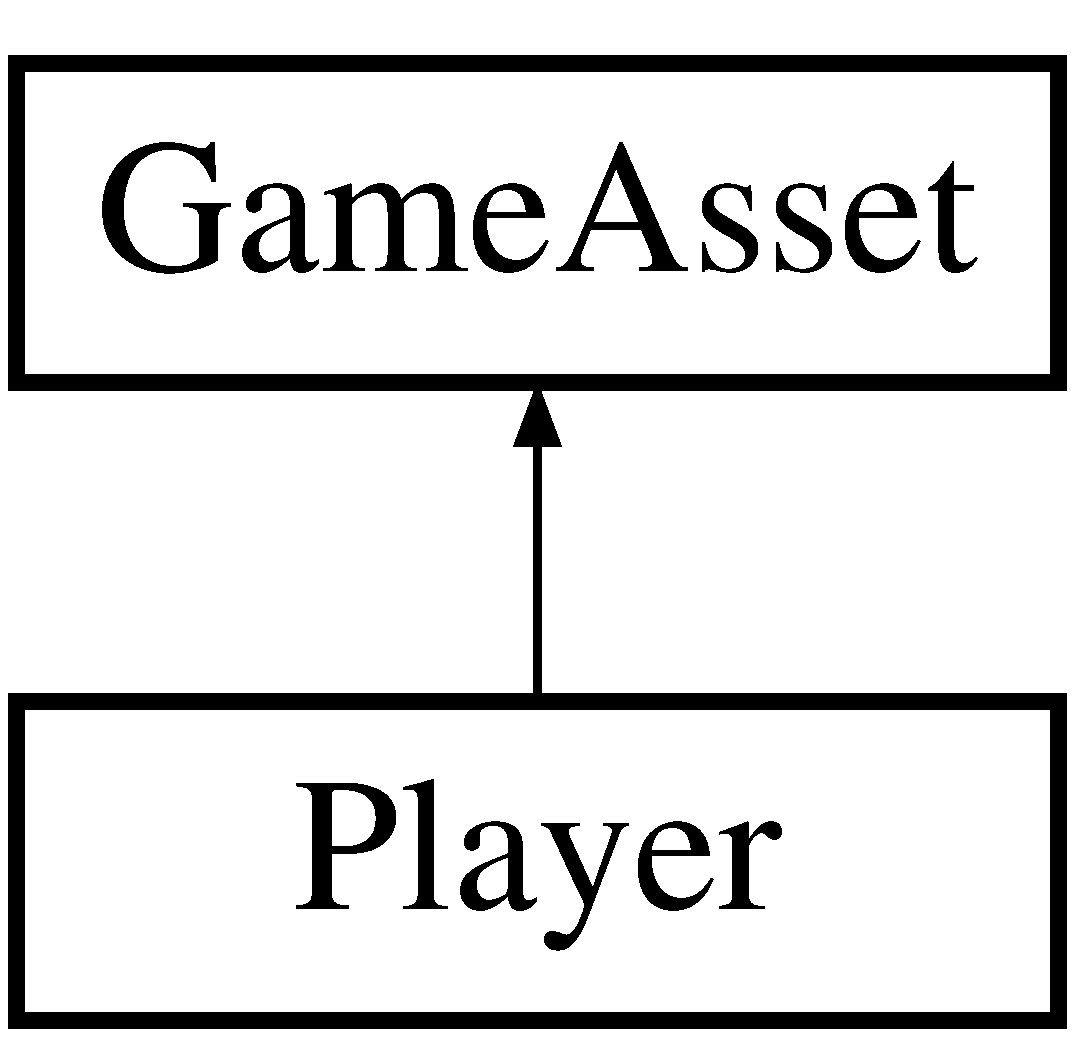
\includegraphics[height=2.000000cm]{classPlayer}
\end{center}
\end{figure}
\subsection*{Public Types}
\begin{DoxyCompactItemize}
\item 
enum \hyperlink{classPlayer_a861f91cf755f14d4d7001edbc1c79980}{vertices} \{ \hyperlink{classPlayer_a861f91cf755f14d4d7001edbc1c79980aa7d37123327782f87ebdfc1603947128}{F0}, 
\hyperlink{classPlayer_a861f91cf755f14d4d7001edbc1c79980a1fc1b1ec99eda01d44d9db82506f8d38}{F1}, 
\hyperlink{classPlayer_a861f91cf755f14d4d7001edbc1c79980a4cf8b3b1f9c2d77553f516a958f74298}{F2}, 
\hyperlink{classPlayer_a861f91cf755f14d4d7001edbc1c79980a369182dcb6e960c07f8d437ef59364df}{F3}
 \}
\end{DoxyCompactItemize}
\subsection*{Public Member Functions}
\begin{DoxyCompactItemize}
\item 
\hyperlink{classPlayer_affe0cc3cb714f6deb4e62f0c0d3f1fd8}{Player} ()
\item 
\hyperlink{classPlayer_a741be2b6a788863970c210081efb2102}{Player} (float x, float y, float z)
\item 
\hyperlink{classPlayer_a749d2c00e1fe0f5c2746f7505a58c062}{$\sim$\-Player} ()
\item 
virtual void \hyperlink{classPlayer_aeeb28c46b0ea75a0a85cbc4c71fccde9}{inc\-Score} (double points)
\item 
virtual void \hyperlink{classPlayer_a6ec12ce91eed06eaf794c663824a752e}{move} (double moving)
\item 
virtual double \hyperlink{classPlayer_aaaa378f4c5cdf0b85dd219cb1fcd4204}{get\-Ammo} ()
\item 
virtual double \hyperlink{classPlayer_ac6605cc08fc355909e44048fb52d7313}{get\-Ammo\-Rate} ()
\item 
virtual void \hyperlink{classPlayer_a6cbd4745a789166da1eb1b7f726fd2ef}{change\-Ammo} (int ammo\-Val)
\item 
virtual void \hyperlink{classPlayer_a640b10aecddb6182bffc7de94b776653}{player\-Invulnerable} ()
\item 
virtual void \hyperlink{classPlayer_af43a2209a8501246dbf2829fac976680}{player\-Vulnerable} ()
\item 
virtual void \hyperlink{classPlayer_a82c3476f3e65a4e2ac6bcd040771bdd4}{update} ()
\item 
virtual void \hyperlink{classPlayer_ac18c9d30d2997765321c62030a4b20b7}{draw} ()
\item 
virtual void \hyperlink{classPlayer_a883c81df5be3b931ecfa6c8de08acfbd}{clean} ()
\end{DoxyCompactItemize}
\subsection*{Public Attributes}
\begin{DoxyCompactItemize}
\item 
int \hyperlink{classPlayer_a689b73da19dd6d6932ffeb5d766709e6}{Ammo}
\item 
double \hyperlink{classPlayer_a38b0bf5bc8ff6e571922d4b51d2aa291}{ammo\-Respawn}
\item 
bool \hyperlink{classPlayer_a16e6b8b49d2f4433e07db406cea1fea5}{invulnerable}
\end{DoxyCompactItemize}
\subsection*{Additional Inherited Members}


\subsection{Detailed Description}


Definition at line 7 of file Player.\-h.



\subsection{Member Enumeration Documentation}
\hypertarget{classPlayer_a861f91cf755f14d4d7001edbc1c79980}{\index{Player@{Player}!vertices@{vertices}}
\index{vertices@{vertices}!Player@{Player}}
\subsubsection[{vertices}]{\setlength{\rightskip}{0pt plus 5cm}enum {\bf Player\-::vertices}}}\label{classPlayer_a861f91cf755f14d4d7001edbc1c79980}
\begin{Desc}
\item[Enumerator]\par
\begin{description}
\index{F0@{F0}!Player@{Player}}\index{Player@{Player}!F0@{F0}}\item[{\em 
\hypertarget{classPlayer_a861f91cf755f14d4d7001edbc1c79980aa7d37123327782f87ebdfc1603947128}{F0}\label{classPlayer_a861f91cf755f14d4d7001edbc1c79980aa7d37123327782f87ebdfc1603947128}
}]\index{F1@{F1}!Player@{Player}}\index{Player@{Player}!F1@{F1}}\item[{\em 
\hypertarget{classPlayer_a861f91cf755f14d4d7001edbc1c79980a1fc1b1ec99eda01d44d9db82506f8d38}{F1}\label{classPlayer_a861f91cf755f14d4d7001edbc1c79980a1fc1b1ec99eda01d44d9db82506f8d38}
}]\index{F2@{F2}!Player@{Player}}\index{Player@{Player}!F2@{F2}}\item[{\em 
\hypertarget{classPlayer_a861f91cf755f14d4d7001edbc1c79980a4cf8b3b1f9c2d77553f516a958f74298}{F2}\label{classPlayer_a861f91cf755f14d4d7001edbc1c79980a4cf8b3b1f9c2d77553f516a958f74298}
}]\index{F3@{F3}!Player@{Player}}\index{Player@{Player}!F3@{F3}}\item[{\em 
\hypertarget{classPlayer_a861f91cf755f14d4d7001edbc1c79980a369182dcb6e960c07f8d437ef59364df}{F3}\label{classPlayer_a861f91cf755f14d4d7001edbc1c79980a369182dcb6e960c07f8d437ef59364df}
}]\end{description}
\end{Desc}


Definition at line 37 of file Player.\-h.


\begin{DoxyCode}
37                 \{
38     \hyperlink{classPlayer_a861f91cf755f14d4d7001edbc1c79980aa7d37123327782f87ebdfc1603947128}{F0}, \hyperlink{classPlayer_a861f91cf755f14d4d7001edbc1c79980a1fc1b1ec99eda01d44d9db82506f8d38}{F1}, \hyperlink{classPlayer_a861f91cf755f14d4d7001edbc1c79980a4cf8b3b1f9c2d77553f516a958f74298}{F2}, \hyperlink{classPlayer_a861f91cf755f14d4d7001edbc1c79980a369182dcb6e960c07f8d437ef59364df}{F3}, 
39   \};
\end{DoxyCode}


\subsection{Constructor \& Destructor Documentation}
\hypertarget{classPlayer_affe0cc3cb714f6deb4e62f0c0d3f1fd8}{\index{Player@{Player}!Player@{Player}}
\index{Player@{Player}!Player@{Player}}
\subsubsection[{Player}]{\setlength{\rightskip}{0pt plus 5cm}Player\-::\-Player (
\begin{DoxyParamCaption}
{}
\end{DoxyParamCaption}
)}}\label{classPlayer_affe0cc3cb714f6deb4e62f0c0d3f1fd8}


Definition at line 3 of file Player.\-cpp.


\begin{DoxyCode}
4   : \hyperlink{classGameAsset_a9c96b0bafa2b6973a2e8c09bf51c52ec}{GameAsset}(
5           \textcolor{keywordtype}{string}(\textcolor{stringliteral}{"CubeRacer/shaders/hello-gl.v.glsl"})
6           , \textcolor{keywordtype}{string}(\textcolor{stringliteral}{"CubeRacer/shaders/player-gl.f.glsl"})
7           )
8 \{
9   \hyperlink{classPlayer_affe0cc3cb714f6deb4e62f0c0d3f1fd8}{Player}(0, 0, 0);
10 \}
\end{DoxyCode}
\hypertarget{classPlayer_a741be2b6a788863970c210081efb2102}{\index{Player@{Player}!Player@{Player}}
\index{Player@{Player}!Player@{Player}}
\subsubsection[{Player}]{\setlength{\rightskip}{0pt plus 5cm}Player\-::\-Player (
\begin{DoxyParamCaption}
\item[{float}]{x, }
\item[{float}]{y, }
\item[{float}]{z}
\end{DoxyParamCaption}
)}}\label{classPlayer_a741be2b6a788863970c210081efb2102}


Definition at line 12 of file Player.\-cpp.


\begin{DoxyCode}
12                                        : \hyperlink{classPlayer_a689b73da19dd6d6932ffeb5d766709e6}{Ammo}(3) , \hyperlink{classPlayer_a38b0bf5bc8ff6e571922d4b51d2aa291}{ammoRespawn}(2.0) , score(0) , 
      \hyperlink{classPlayer_a16e6b8b49d2f4433e07db406cea1fea5}{invulnerable}(\textcolor{keyword}{false}) \{
13 
14   \textcolor{comment}{// A default "unit" cube}
15   \hyperlink{classGameAsset_a3e8d7dc58d3d4efafbbce1536b78dbc7}{num\_vertices} = 4;
16   \hyperlink{classGameAsset_aae4d864335c2eca685cc86602881cd18}{num\_triangles} = 4;
17   \hyperlink{classGameAsset_ae1d682ecf84d9cd3f91a8c870acf2777}{g\_vertex\_buffer\_data} = \textcolor{keyword}{new} GLfloat[\hyperlink{classGameAsset_a3e8d7dc58d3d4efafbbce1536b78dbc7}{num\_vertices} * 3]\{
18 
19   \textcolor{comment}{//     x      y     z}
20     -0.5, -0.5, -0.5, \textcolor{comment}{//F - 0  //base of the triangle player}
21      0.5, -0.5, -0.5, \textcolor{comment}{//F - 1}
22      0.0, -0.5,  0.5, \textcolor{comment}{//F - 2}
23      0.0,  0.0,  0.0, \textcolor{comment}{//F - 3  //top point og the triangle player}
24     
25 \}; \textcolor{comment}{// three points per vertex}
26 
27   \hyperlink{classGameAsset_ab859393c9158c8bda39cd100475fee25}{g\_element\_buffer\_data} = \textcolor{keyword}{new} GLushort[\hyperlink{classGameAsset_aae4d864335c2eca685cc86602881cd18}{num\_triangles} * 3]\{
28 
29     \hyperlink{classPlayer_a861f91cf755f14d4d7001edbc1c79980aa7d37123327782f87ebdfc1603947128}{F0}, \hyperlink{classPlayer_a861f91cf755f14d4d7001edbc1c79980a1fc1b1ec99eda01d44d9db82506f8d38}{F1}, \hyperlink{classPlayer_a861f91cf755f14d4d7001edbc1c79980a4cf8b3b1f9c2d77553f516a958f74298}{F2},   \textcolor{comment}{//Base}
30     \hyperlink{classPlayer_a861f91cf755f14d4d7001edbc1c79980aa7d37123327782f87ebdfc1603947128}{F0}, \hyperlink{classPlayer_a861f91cf755f14d4d7001edbc1c79980a1fc1b1ec99eda01d44d9db82506f8d38}{F1}, \hyperlink{classPlayer_a861f91cf755f14d4d7001edbc1c79980a369182dcb6e960c07f8d437ef59364df}{F3},   \textcolor{comment}{//Back}
31     \hyperlink{classPlayer_a861f91cf755f14d4d7001edbc1c79980a1fc1b1ec99eda01d44d9db82506f8d38}{F1}, \hyperlink{classPlayer_a861f91cf755f14d4d7001edbc1c79980a4cf8b3b1f9c2d77553f516a958f74298}{F2}, \hyperlink{classPlayer_a861f91cf755f14d4d7001edbc1c79980a369182dcb6e960c07f8d437ef59364df}{F3},   \textcolor{comment}{//RightSide}
32     \hyperlink{classPlayer_a861f91cf755f14d4d7001edbc1c79980a4cf8b3b1f9c2d77553f516a958f74298}{F2}, \hyperlink{classPlayer_a861f91cf755f14d4d7001edbc1c79980aa7d37123327782f87ebdfc1603947128}{F0}, F0    \textcolor{comment}{//LeftSide}
33     
34 \}; \textcolor{comment}{// three vertices per triangle}
35 
36   \hyperlink{classGameAsset_a3444a096fed505b1740bedc95e2cfa6c}{bbox}.reset();
37   \hyperlink{classGameAsset_a3444a096fed505b1740bedc95e2cfa6c}{bbox} = shared\_ptr<BoundingBox>(\textcolor{keyword}{new} \hyperlink{classBoundingBox}{BoundingBox}(\hyperlink{classVectormath_1_1Aos_1_1Point3}{Point3}(x, y, z), 1.0, 1.0, 1.0));
38 
39   \hyperlink{classGameAsset_aa26d85233ece476d599adf90074e9568}{make\_resources}();
40 \}
\end{DoxyCode}
\hypertarget{classPlayer_a749d2c00e1fe0f5c2746f7505a58c062}{\index{Player@{Player}!$\sim$\-Player@{$\sim$\-Player}}
\index{$\sim$\-Player@{$\sim$\-Player}!Player@{Player}}
\subsubsection[{$\sim$\-Player}]{\setlength{\rightskip}{0pt plus 5cm}Player\-::$\sim$\-Player (
\begin{DoxyParamCaption}
{}
\end{DoxyParamCaption}
)}}\label{classPlayer_a749d2c00e1fe0f5c2746f7505a58c062}


Definition at line 42 of file Player.\-cpp.


\begin{DoxyCode}
42                 \{
43   \textcolor{comment}{// TODO: do something nice and fun here.}
44 \}
\end{DoxyCode}


\subsection{Member Function Documentation}
\hypertarget{classPlayer_a6cbd4745a789166da1eb1b7f726fd2ef}{\index{Player@{Player}!change\-Ammo@{change\-Ammo}}
\index{change\-Ammo@{change\-Ammo}!Player@{Player}}
\subsubsection[{change\-Ammo}]{\setlength{\rightskip}{0pt plus 5cm}void Player\-::change\-Ammo (
\begin{DoxyParamCaption}
\item[{int}]{ammo\-Val}
\end{DoxyParamCaption}
)\hspace{0.3cm}{\ttfamily [virtual]}}}\label{classPlayer_a6cbd4745a789166da1eb1b7f726fd2ef}


Definition at line 69 of file Player.\-cpp.


\begin{DoxyCode}
69                                   \{
70   \hyperlink{classPlayer_a689b73da19dd6d6932ffeb5d766709e6}{Ammo} = \hyperlink{classPlayer_a689b73da19dd6d6932ffeb5d766709e6}{Ammo} + ammoVal;
71 \}
\end{DoxyCode}
\hypertarget{classPlayer_a883c81df5be3b931ecfa6c8de08acfbd}{\index{Player@{Player}!clean@{clean}}
\index{clean@{clean}!Player@{Player}}
\subsubsection[{clean}]{\setlength{\rightskip}{0pt plus 5cm}void Player\-::clean (
\begin{DoxyParamCaption}
{}
\end{DoxyParamCaption}
)\hspace{0.3cm}{\ttfamily [virtual]}}}\label{classPlayer_a883c81df5be3b931ecfa6c8de08acfbd}


Implements \hyperlink{classGameAsset_abbea962eaa63a813949b834778b7483e}{Game\-Asset}.



Definition at line 95 of file Player.\-cpp.


\begin{DoxyCode}
95 \{ \}
\end{DoxyCode}
\hypertarget{classPlayer_ac18c9d30d2997765321c62030a4b20b7}{\index{Player@{Player}!draw@{draw}}
\index{draw@{draw}!Player@{Player}}
\subsubsection[{draw}]{\setlength{\rightskip}{0pt plus 5cm}void Player\-::draw (
\begin{DoxyParamCaption}
{}
\end{DoxyParamCaption}
)\hspace{0.3cm}{\ttfamily [virtual]}}}\label{classPlayer_ac18c9d30d2997765321c62030a4b20b7}


Reimplemented from \hyperlink{classGameAsset_a2d7e18a8f1dd8ba89ed1bd14f2affeab}{Game\-Asset}.



Definition at line 91 of file Player.\-cpp.


\begin{DoxyCode}
91                   \{
92   \hyperlink{classGameAsset_a2d7e18a8f1dd8ba89ed1bd14f2affeab}{GameAsset::draw}();
93 \}
\end{DoxyCode}
\hypertarget{classPlayer_aaaa378f4c5cdf0b85dd219cb1fcd4204}{\index{Player@{Player}!get\-Ammo@{get\-Ammo}}
\index{get\-Ammo@{get\-Ammo}!Player@{Player}}
\subsubsection[{get\-Ammo}]{\setlength{\rightskip}{0pt plus 5cm}double Player\-::get\-Ammo (
\begin{DoxyParamCaption}
{}
\end{DoxyParamCaption}
)\hspace{0.3cm}{\ttfamily [virtual]}}}\label{classPlayer_aaaa378f4c5cdf0b85dd219cb1fcd4204}


Definition at line 61 of file Player.\-cpp.


\begin{DoxyCode}
61                       \{
62   \textcolor{keywordflow}{return} \hyperlink{classPlayer_a689b73da19dd6d6932ffeb5d766709e6}{Ammo};
63 \}
\end{DoxyCode}
\hypertarget{classPlayer_ac6605cc08fc355909e44048fb52d7313}{\index{Player@{Player}!get\-Ammo\-Rate@{get\-Ammo\-Rate}}
\index{get\-Ammo\-Rate@{get\-Ammo\-Rate}!Player@{Player}}
\subsubsection[{get\-Ammo\-Rate}]{\setlength{\rightskip}{0pt plus 5cm}double Player\-::get\-Ammo\-Rate (
\begin{DoxyParamCaption}
{}
\end{DoxyParamCaption}
)\hspace{0.3cm}{\ttfamily [virtual]}}}\label{classPlayer_ac6605cc08fc355909e44048fb52d7313}


Definition at line 65 of file Player.\-cpp.


\begin{DoxyCode}
65                           \{
66   \textcolor{keywordflow}{return} \hyperlink{classPlayer_a38b0bf5bc8ff6e571922d4b51d2aa291}{ammoRespawn};
67 \}
\end{DoxyCode}
\hypertarget{classPlayer_aeeb28c46b0ea75a0a85cbc4c71fccde9}{\index{Player@{Player}!inc\-Score@{inc\-Score}}
\index{inc\-Score@{inc\-Score}!Player@{Player}}
\subsubsection[{inc\-Score}]{\setlength{\rightskip}{0pt plus 5cm}void Player\-::inc\-Score (
\begin{DoxyParamCaption}
\item[{double}]{points}
\end{DoxyParamCaption}
)\hspace{0.3cm}{\ttfamily [virtual]}}}\label{classPlayer_aeeb28c46b0ea75a0a85cbc4c71fccde9}


Definition at line 87 of file Player.\-cpp.


\begin{DoxyCode}
87                                    \{
88   score = score + points;
89 \}
\end{DoxyCode}
\hypertarget{classPlayer_a6ec12ce91eed06eaf794c663824a752e}{\index{Player@{Player}!move@{move}}
\index{move@{move}!Player@{Player}}
\subsubsection[{move}]{\setlength{\rightskip}{0pt plus 5cm}void Player\-::move (
\begin{DoxyParamCaption}
\item[{double}]{moving}
\end{DoxyParamCaption}
)\hspace{0.3cm}{\ttfamily [virtual]}}}\label{classPlayer_a6ec12ce91eed06eaf794c663824a752e}


Definition at line 81 of file Player.\-cpp.


\begin{DoxyCode}
81                               \{
82   shared\_ptr<Point3> \hyperlink{classPlayer_a6ec12ce91eed06eaf794c663824a752e}{move} = this->\hyperlink{classGameAsset_a3444a096fed505b1740bedc95e2cfa6c}{bbox}->getCentre();
83   *move = \hyperlink{classVectormath_1_1Aos_1_1Point3}{Point3}(move->getX() + moving, 0.0, 0.0);
84   move.reset();
85 \}
\end{DoxyCode}
\hypertarget{classPlayer_a640b10aecddb6182bffc7de94b776653}{\index{Player@{Player}!player\-Invulnerable@{player\-Invulnerable}}
\index{player\-Invulnerable@{player\-Invulnerable}!Player@{Player}}
\subsubsection[{player\-Invulnerable}]{\setlength{\rightskip}{0pt plus 5cm}void Player\-::player\-Invulnerable (
\begin{DoxyParamCaption}
{}
\end{DoxyParamCaption}
)\hspace{0.3cm}{\ttfamily [virtual]}}}\label{classPlayer_a640b10aecddb6182bffc7de94b776653}


Definition at line 73 of file Player.\-cpp.


\begin{DoxyCode}
73                                \{
74   \hyperlink{classPlayer_a16e6b8b49d2f4433e07db406cea1fea5}{invulnerable} = \textcolor{keyword}{true};
75 \}
\end{DoxyCode}
\hypertarget{classPlayer_af43a2209a8501246dbf2829fac976680}{\index{Player@{Player}!player\-Vulnerable@{player\-Vulnerable}}
\index{player\-Vulnerable@{player\-Vulnerable}!Player@{Player}}
\subsubsection[{player\-Vulnerable}]{\setlength{\rightskip}{0pt plus 5cm}void Player\-::player\-Vulnerable (
\begin{DoxyParamCaption}
{}
\end{DoxyParamCaption}
)\hspace{0.3cm}{\ttfamily [virtual]}}}\label{classPlayer_af43a2209a8501246dbf2829fac976680}


Definition at line 77 of file Player.\-cpp.


\begin{DoxyCode}
77                              \{
78   \hyperlink{classPlayer_a16e6b8b49d2f4433e07db406cea1fea5}{invulnerable} = \textcolor{keyword}{false};
79 \}
\end{DoxyCode}
\hypertarget{classPlayer_a82c3476f3e65a4e2ac6bcd040771bdd4}{\index{Player@{Player}!update@{update}}
\index{update@{update}!Player@{Player}}
\subsubsection[{update}]{\setlength{\rightskip}{0pt plus 5cm}void Player\-::update (
\begin{DoxyParamCaption}
{}
\end{DoxyParamCaption}
)\hspace{0.3cm}{\ttfamily [virtual]}}}\label{classPlayer_a82c3476f3e65a4e2ac6bcd040771bdd4}


Implements \hyperlink{classGameAsset_a42688ec8f02e201eaaa01e74a112083f}{Game\-Asset}.



Definition at line 46 of file Player.\-cpp.


\begin{DoxyCode}
46                     \{
47   \textcolor{keywordflow}{if} (\hyperlink{classGameAsset_aebf93ae52dc7fabbb6ec7edaadf915d0}{isAlive}) 
48   \{
49     score += 0.1;
50     \textcolor{comment}{//cout << score << endl;}
51   \}
52   \textcolor{keywordflow}{else}
53   \{ 
54     cout << \textcolor{stringliteral}{"You have died."} << endl;
55     cout << \textcolor{stringliteral}{"Your Score: "} << score << endl;
56     this->\hyperlink{classPlayer_a883c81df5be3b931ecfa6c8de08acfbd}{clean}();
57     SDL\_Quit();
58   \}
59 \}
\end{DoxyCode}


\subsection{Member Data Documentation}
\hypertarget{classPlayer_a689b73da19dd6d6932ffeb5d766709e6}{\index{Player@{Player}!Ammo@{Ammo}}
\index{Ammo@{Ammo}!Player@{Player}}
\subsubsection[{Ammo}]{\setlength{\rightskip}{0pt plus 5cm}int Player\-::\-Ammo}}\label{classPlayer_a689b73da19dd6d6932ffeb5d766709e6}


Definition at line 33 of file Player.\-h.

\hypertarget{classPlayer_a38b0bf5bc8ff6e571922d4b51d2aa291}{\index{Player@{Player}!ammo\-Respawn@{ammo\-Respawn}}
\index{ammo\-Respawn@{ammo\-Respawn}!Player@{Player}}
\subsubsection[{ammo\-Respawn}]{\setlength{\rightskip}{0pt plus 5cm}double Player\-::ammo\-Respawn}}\label{classPlayer_a38b0bf5bc8ff6e571922d4b51d2aa291}


Definition at line 34 of file Player.\-h.

\hypertarget{classPlayer_a16e6b8b49d2f4433e07db406cea1fea5}{\index{Player@{Player}!invulnerable@{invulnerable}}
\index{invulnerable@{invulnerable}!Player@{Player}}
\subsubsection[{invulnerable}]{\setlength{\rightskip}{0pt plus 5cm}bool Player\-::invulnerable}}\label{classPlayer_a16e6b8b49d2f4433e07db406cea1fea5}


Definition at line 35 of file Player.\-h.



The documentation for this class was generated from the following files\-:\begin{DoxyCompactItemize}
\item 
/home/sam/\-Cube\-Racer/src/\hyperlink{Player_8h}{Player.\-h}\item 
/home/sam/\-Cube\-Racer/src/\hyperlink{Player_8cpp}{Player.\-cpp}\end{DoxyCompactItemize}

\hypertarget{classVectormath_1_1Aos_1_1Point3}{\section{Vectormath\-:\-:Aos\-:\-:Point3 Class Reference}
\label{classVectormath_1_1Aos_1_1Point3}\index{Vectormath\-::\-Aos\-::\-Point3@{Vectormath\-::\-Aos\-::\-Point3}}
}


{\ttfamily \#include $<$vectormath\-\_\-aos.\-h$>$}

\subsection*{Public Member Functions}
\begin{DoxyCompactItemize}
\item 
\hyperlink{classVectormath_1_1Aos_1_1Point3_a973eba31897962191c032bc585530c49}{Point3} ()
\item 
\hyperlink{classVectormath_1_1Aos_1_1Point3_a03dfaf1fbce8f78dc3569e57034a3fc8}{Point3} (const \hyperlink{classVectormath_1_1Aos_1_1Point3}{Point3} \&pnt)
\item 
\hyperlink{classVectormath_1_1Aos_1_1Point3_a74641a8ac1d99934fea99880a06b58db}{Point3} (float x, float y, float z)
\item 
\hyperlink{classVectormath_1_1Aos_1_1Point3_a0b286492bfd84978c68d9c89c3756596}{Point3} (const \hyperlink{classVectormath_1_1Aos_1_1Vector3}{Vector3} \&vec)
\item 
\hyperlink{classVectormath_1_1Aos_1_1Point3_a52800d18e22d003682c5c2bc9dd3cef4}{Point3} (float scalar)
\item 
\hyperlink{classVectormath_1_1Aos_1_1Point3}{Point3} \& \hyperlink{classVectormath_1_1Aos_1_1Point3_a411758d7b078206e477e0f9d681465ff}{operator=} (const \hyperlink{classVectormath_1_1Aos_1_1Point3}{Point3} \&pnt)
\item 
\hyperlink{classVectormath_1_1Aos_1_1Point3}{Point3} \& \hyperlink{classVectormath_1_1Aos_1_1Point3_a5248262aa8bb9da9e47389788175aa3c}{set\-X} (float x)
\item 
\hyperlink{classVectormath_1_1Aos_1_1Point3}{Point3} \& \hyperlink{classVectormath_1_1Aos_1_1Point3_a3306a2e2e47eb1a9f912f53b57ef8a6c}{set\-Y} (float y)
\item 
\hyperlink{classVectormath_1_1Aos_1_1Point3}{Point3} \& \hyperlink{classVectormath_1_1Aos_1_1Point3_acc8a1cc561400ebde5d83df3999afa5c}{set\-Z} (float z)
\item 
float \hyperlink{classVectormath_1_1Aos_1_1Point3_aae02e04a14cd7d4194ca681df958e08f}{get\-X} () const 
\item 
float \hyperlink{classVectormath_1_1Aos_1_1Point3_a6d06ef54d34f7552680d1e7d672ab473}{get\-Y} () const 
\item 
float \hyperlink{classVectormath_1_1Aos_1_1Point3_ad83252a573e61cff750b1e93420d469f}{get\-Z} () const 
\item 
\hyperlink{classVectormath_1_1Aos_1_1Point3}{Point3} \& \hyperlink{classVectormath_1_1Aos_1_1Point3_ad526b87fcb32481172843961a24c998e}{set\-Elem} (int idx, float value)
\item 
float \hyperlink{classVectormath_1_1Aos_1_1Point3_a799aaab8cc96e46dffc1f14475d00a11}{get\-Elem} (int idx) const 
\item 
float \& \hyperlink{classVectormath_1_1Aos_1_1Point3_a9199103ca52600d52dee2852dfa56e60}{operator\mbox{[}$\,$\mbox{]}} (int idx)
\item 
float \hyperlink{classVectormath_1_1Aos_1_1Point3_a3efc9e792f42d04bfb88b440c2b7f33b}{operator\mbox{[}$\,$\mbox{]}} (int idx) const 
\item 
const \hyperlink{classVectormath_1_1Aos_1_1Vector3}{Vector3} \hyperlink{classVectormath_1_1Aos_1_1Point3_ac110665a00116cf76309f2d4a898fd92}{operator-\/} (const \hyperlink{classVectormath_1_1Aos_1_1Point3}{Point3} \&pnt) const 
\item 
const \hyperlink{classVectormath_1_1Aos_1_1Point3}{Point3} \hyperlink{classVectormath_1_1Aos_1_1Point3_abe36c3385029863afc4ec28129dd5430}{operator+} (const \hyperlink{classVectormath_1_1Aos_1_1Vector3}{Vector3} \&vec) const 
\item 
const \hyperlink{classVectormath_1_1Aos_1_1Point3}{Point3} \hyperlink{classVectormath_1_1Aos_1_1Point3_ab46ebdacfa7955ce5ba542add038c1bb}{operator-\/} (const \hyperlink{classVectormath_1_1Aos_1_1Vector3}{Vector3} \&vec) const 
\item 
\hyperlink{classVectormath_1_1Aos_1_1Point3}{Point3} \& \hyperlink{classVectormath_1_1Aos_1_1Point3_ab815d7df7f54305c47288eeef62419e4}{operator+=} (const \hyperlink{classVectormath_1_1Aos_1_1Vector3}{Vector3} \&vec)
\item 
\hyperlink{classVectormath_1_1Aos_1_1Point3}{Point3} \& \hyperlink{classVectormath_1_1Aos_1_1Point3_a96d9cf86705dd4a76051958d372819ca}{operator-\/=} (const \hyperlink{classVectormath_1_1Aos_1_1Vector3}{Vector3} \&vec)
\end{DoxyCompactItemize}


\subsection{Detailed Description}


Definition at line 645 of file vectormath\-\_\-aos.\-h.



\subsection{Constructor \& Destructor Documentation}
\hypertarget{classVectormath_1_1Aos_1_1Point3_a973eba31897962191c032bc585530c49}{\index{Vectormath\-::\-Aos\-::\-Point3@{Vectormath\-::\-Aos\-::\-Point3}!Point3@{Point3}}
\index{Point3@{Point3}!Vectormath::Aos::Point3@{Vectormath\-::\-Aos\-::\-Point3}}
\subsubsection[{Point3}]{\setlength{\rightskip}{0pt plus 5cm}Vectormath\-::\-Aos\-::\-Point3\-::\-Point3 (
\begin{DoxyParamCaption}
{}
\end{DoxyParamCaption}
)\hspace{0.3cm}{\ttfamily [inline]}}}\label{classVectormath_1_1Aos_1_1Point3_a973eba31897962191c032bc585530c49}


Definition at line 657 of file vectormath\-\_\-aos.\-h.


\begin{DoxyCode}
657 \{ \};
\end{DoxyCode}
\hypertarget{classVectormath_1_1Aos_1_1Point3_a03dfaf1fbce8f78dc3569e57034a3fc8}{\index{Vectormath\-::\-Aos\-::\-Point3@{Vectormath\-::\-Aos\-::\-Point3}!Point3@{Point3}}
\index{Point3@{Point3}!Vectormath::Aos::Point3@{Vectormath\-::\-Aos\-::\-Point3}}
\subsubsection[{Point3}]{\setlength{\rightskip}{0pt plus 5cm}Vectormath\-::\-Aos\-::\-Point3\-::\-Point3 (
\begin{DoxyParamCaption}
\item[{const {\bf Point3} \&}]{pnt}
\end{DoxyParamCaption}
)\hspace{0.3cm}{\ttfamily [inline]}}}\label{classVectormath_1_1Aos_1_1Point3_a03dfaf1fbce8f78dc3569e57034a3fc8}


Definition at line 1047 of file vec\-\_\-aos.\-h.


\begin{DoxyCode}
1048 \{
1049     mX = pnt.mX;
1050     mY = pnt.mY;
1051     mZ = pnt.mZ;
1052 \}
\end{DoxyCode}
\hypertarget{classVectormath_1_1Aos_1_1Point3_a74641a8ac1d99934fea99880a06b58db}{\index{Vectormath\-::\-Aos\-::\-Point3@{Vectormath\-::\-Aos\-::\-Point3}!Point3@{Point3}}
\index{Point3@{Point3}!Vectormath::Aos::Point3@{Vectormath\-::\-Aos\-::\-Point3}}
\subsubsection[{Point3}]{\setlength{\rightskip}{0pt plus 5cm}Vectormath\-::\-Aos\-::\-Point3\-::\-Point3 (
\begin{DoxyParamCaption}
\item[{float}]{x, }
\item[{float}]{y, }
\item[{float}]{z}
\end{DoxyParamCaption}
)\hspace{0.3cm}{\ttfamily [inline]}}}\label{classVectormath_1_1Aos_1_1Point3_a74641a8ac1d99934fea99880a06b58db}


Definition at line 1054 of file vec\-\_\-aos.\-h.


\begin{DoxyCode}
1055 \{
1056     mX = \_x;
1057     mY = \_y;
1058     mZ = \_z;
1059 \}
\end{DoxyCode}
\hypertarget{classVectormath_1_1Aos_1_1Point3_a0b286492bfd84978c68d9c89c3756596}{\index{Vectormath\-::\-Aos\-::\-Point3@{Vectormath\-::\-Aos\-::\-Point3}!Point3@{Point3}}
\index{Point3@{Point3}!Vectormath::Aos::Point3@{Vectormath\-::\-Aos\-::\-Point3}}
\subsubsection[{Point3}]{\setlength{\rightskip}{0pt plus 5cm}Vectormath\-::\-Aos\-::\-Point3\-::\-Point3 (
\begin{DoxyParamCaption}
\item[{const {\bf Vector3} \&}]{vec}
\end{DoxyParamCaption}
)\hspace{0.3cm}{\ttfamily [inline]}, {\ttfamily [explicit]}}}\label{classVectormath_1_1Aos_1_1Point3_a0b286492bfd84978c68d9c89c3756596}


Definition at line 1061 of file vec\-\_\-aos.\-h.


\begin{DoxyCode}
1062 \{
1063     mX = vec.getX();
1064     mY = vec.getY();
1065     mZ = vec.getZ();
1066 \}
\end{DoxyCode}
\hypertarget{classVectormath_1_1Aos_1_1Point3_a52800d18e22d003682c5c2bc9dd3cef4}{\index{Vectormath\-::\-Aos\-::\-Point3@{Vectormath\-::\-Aos\-::\-Point3}!Point3@{Point3}}
\index{Point3@{Point3}!Vectormath::Aos::Point3@{Vectormath\-::\-Aos\-::\-Point3}}
\subsubsection[{Point3}]{\setlength{\rightskip}{0pt plus 5cm}Vectormath\-::\-Aos\-::\-Point3\-::\-Point3 (
\begin{DoxyParamCaption}
\item[{float}]{scalar}
\end{DoxyParamCaption}
)\hspace{0.3cm}{\ttfamily [inline]}, {\ttfamily [explicit]}}}\label{classVectormath_1_1Aos_1_1Point3_a52800d18e22d003682c5c2bc9dd3cef4}


Definition at line 1068 of file vec\-\_\-aos.\-h.


\begin{DoxyCode}
1069 \{
1070     mX = scalar;
1071     mY = scalar;
1072     mZ = scalar;
1073 \}
\end{DoxyCode}


\subsection{Member Function Documentation}
\hypertarget{classVectormath_1_1Aos_1_1Point3_a799aaab8cc96e46dffc1f14475d00a11}{\index{Vectormath\-::\-Aos\-::\-Point3@{Vectormath\-::\-Aos\-::\-Point3}!get\-Elem@{get\-Elem}}
\index{get\-Elem@{get\-Elem}!Vectormath::Aos::Point3@{Vectormath\-::\-Aos\-::\-Point3}}
\subsubsection[{get\-Elem}]{\setlength{\rightskip}{0pt plus 5cm}float Vectormath\-::\-Aos\-::\-Point3\-::get\-Elem (
\begin{DoxyParamCaption}
\item[{int}]{idx}
\end{DoxyParamCaption}
) const\hspace{0.3cm}{\ttfamily [inline]}}}\label{classVectormath_1_1Aos_1_1Point3_a799aaab8cc96e46dffc1f14475d00a11}


Definition at line 1215 of file vec\-\_\-aos.\-h.


\begin{DoxyCode}
1216 \{
1217     \textcolor{keywordflow}{return} *(&mX + idx);
1218 \}
\end{DoxyCode}
\hypertarget{classVectormath_1_1Aos_1_1Point3_aae02e04a14cd7d4194ca681df958e08f}{\index{Vectormath\-::\-Aos\-::\-Point3@{Vectormath\-::\-Aos\-::\-Point3}!get\-X@{get\-X}}
\index{get\-X@{get\-X}!Vectormath::Aos::Point3@{Vectormath\-::\-Aos\-::\-Point3}}
\subsubsection[{get\-X}]{\setlength{\rightskip}{0pt plus 5cm}float Vectormath\-::\-Aos\-::\-Point3\-::get\-X (
\begin{DoxyParamCaption}
{}
\end{DoxyParamCaption}
) const\hspace{0.3cm}{\ttfamily [inline]}}}\label{classVectormath_1_1Aos_1_1Point3_aae02e04a14cd7d4194ca681df958e08f}


Definition at line 1182 of file vec\-\_\-aos.\-h.


\begin{DoxyCode}
1183 \{
1184     \textcolor{keywordflow}{return} mX;
1185 \}
\end{DoxyCode}
\hypertarget{classVectormath_1_1Aos_1_1Point3_a6d06ef54d34f7552680d1e7d672ab473}{\index{Vectormath\-::\-Aos\-::\-Point3@{Vectormath\-::\-Aos\-::\-Point3}!get\-Y@{get\-Y}}
\index{get\-Y@{get\-Y}!Vectormath::Aos::Point3@{Vectormath\-::\-Aos\-::\-Point3}}
\subsubsection[{get\-Y}]{\setlength{\rightskip}{0pt plus 5cm}float Vectormath\-::\-Aos\-::\-Point3\-::get\-Y (
\begin{DoxyParamCaption}
{}
\end{DoxyParamCaption}
) const\hspace{0.3cm}{\ttfamily [inline]}}}\label{classVectormath_1_1Aos_1_1Point3_a6d06ef54d34f7552680d1e7d672ab473}


Definition at line 1193 of file vec\-\_\-aos.\-h.


\begin{DoxyCode}
1194 \{
1195     \textcolor{keywordflow}{return} mY;
1196 \}
\end{DoxyCode}
\hypertarget{classVectormath_1_1Aos_1_1Point3_ad83252a573e61cff750b1e93420d469f}{\index{Vectormath\-::\-Aos\-::\-Point3@{Vectormath\-::\-Aos\-::\-Point3}!get\-Z@{get\-Z}}
\index{get\-Z@{get\-Z}!Vectormath::Aos::Point3@{Vectormath\-::\-Aos\-::\-Point3}}
\subsubsection[{get\-Z}]{\setlength{\rightskip}{0pt plus 5cm}float Vectormath\-::\-Aos\-::\-Point3\-::get\-Z (
\begin{DoxyParamCaption}
{}
\end{DoxyParamCaption}
) const\hspace{0.3cm}{\ttfamily [inline]}}}\label{classVectormath_1_1Aos_1_1Point3_ad83252a573e61cff750b1e93420d469f}


Definition at line 1204 of file vec\-\_\-aos.\-h.


\begin{DoxyCode}
1205 \{
1206     \textcolor{keywordflow}{return} mZ;
1207 \}
\end{DoxyCode}
\hypertarget{classVectormath_1_1Aos_1_1Point3_abe36c3385029863afc4ec28129dd5430}{\index{Vectormath\-::\-Aos\-::\-Point3@{Vectormath\-::\-Aos\-::\-Point3}!operator+@{operator+}}
\index{operator+@{operator+}!Vectormath::Aos::Point3@{Vectormath\-::\-Aos\-::\-Point3}}
\subsubsection[{operator+}]{\setlength{\rightskip}{0pt plus 5cm}const {\bf Point3} Vectormath\-::\-Aos\-::\-Point3\-::operator+ (
\begin{DoxyParamCaption}
\item[{const {\bf Vector3} \&}]{vec}
\end{DoxyParamCaption}
) const\hspace{0.3cm}{\ttfamily [inline]}}}\label{classVectormath_1_1Aos_1_1Point3_abe36c3385029863afc4ec28129dd5430}


Definition at line 1239 of file vec\-\_\-aos.\-h.


\begin{DoxyCode}
1240 \{
1241     \textcolor{keywordflow}{return} \hyperlink{classVectormath_1_1Aos_1_1Point3_a973eba31897962191c032bc585530c49}{Point3}(
1242         ( mX + vec.getX() ),
1243         ( mY + vec.getY() ),
1244         ( mZ + vec.getZ() )
1245     );
1246 \}
\end{DoxyCode}
\hypertarget{classVectormath_1_1Aos_1_1Point3_ab815d7df7f54305c47288eeef62419e4}{\index{Vectormath\-::\-Aos\-::\-Point3@{Vectormath\-::\-Aos\-::\-Point3}!operator+=@{operator+=}}
\index{operator+=@{operator+=}!Vectormath::Aos::Point3@{Vectormath\-::\-Aos\-::\-Point3}}
\subsubsection[{operator+=}]{\setlength{\rightskip}{0pt plus 5cm}{\bf Point3} \& Vectormath\-::\-Aos\-::\-Point3\-::operator+= (
\begin{DoxyParamCaption}
\item[{const {\bf Vector3} \&}]{vec}
\end{DoxyParamCaption}
)\hspace{0.3cm}{\ttfamily [inline]}}}\label{classVectormath_1_1Aos_1_1Point3_ab815d7df7f54305c47288eeef62419e4}


Definition at line 1257 of file vec\-\_\-aos.\-h.


\begin{DoxyCode}
1258 \{
1259     *\textcolor{keyword}{this} = *\textcolor{keyword}{this} + vec;
1260     \textcolor{keywordflow}{return} *\textcolor{keyword}{this};
1261 \}
\end{DoxyCode}
\hypertarget{classVectormath_1_1Aos_1_1Point3_ac110665a00116cf76309f2d4a898fd92}{\index{Vectormath\-::\-Aos\-::\-Point3@{Vectormath\-::\-Aos\-::\-Point3}!operator-\/@{operator-\/}}
\index{operator-\/@{operator-\/}!Vectormath::Aos::Point3@{Vectormath\-::\-Aos\-::\-Point3}}
\subsubsection[{operator-\/}]{\setlength{\rightskip}{0pt plus 5cm}const {\bf Vector3} Vectormath\-::\-Aos\-::\-Point3\-::operator-\/ (
\begin{DoxyParamCaption}
\item[{const {\bf Point3} \&}]{pnt}
\end{DoxyParamCaption}
) const\hspace{0.3cm}{\ttfamily [inline]}}}\label{classVectormath_1_1Aos_1_1Point3_ac110665a00116cf76309f2d4a898fd92}


Definition at line 1230 of file vec\-\_\-aos.\-h.


\begin{DoxyCode}
1231 \{
1232     \textcolor{keywordflow}{return} Vector3(
1233         ( mX - pnt.mX ),
1234         ( mY - pnt.mY ),
1235         ( mZ - pnt.mZ )
1236     );
1237 \}
\end{DoxyCode}
\hypertarget{classVectormath_1_1Aos_1_1Point3_ab46ebdacfa7955ce5ba542add038c1bb}{\index{Vectormath\-::\-Aos\-::\-Point3@{Vectormath\-::\-Aos\-::\-Point3}!operator-\/@{operator-\/}}
\index{operator-\/@{operator-\/}!Vectormath::Aos::Point3@{Vectormath\-::\-Aos\-::\-Point3}}
\subsubsection[{operator-\/}]{\setlength{\rightskip}{0pt plus 5cm}const {\bf Point3} Vectormath\-::\-Aos\-::\-Point3\-::operator-\/ (
\begin{DoxyParamCaption}
\item[{const {\bf Vector3} \&}]{vec}
\end{DoxyParamCaption}
) const\hspace{0.3cm}{\ttfamily [inline]}}}\label{classVectormath_1_1Aos_1_1Point3_ab46ebdacfa7955ce5ba542add038c1bb}


Definition at line 1248 of file vec\-\_\-aos.\-h.


\begin{DoxyCode}
1249 \{
1250     \textcolor{keywordflow}{return} \hyperlink{classVectormath_1_1Aos_1_1Point3_a973eba31897962191c032bc585530c49}{Point3}(
1251         ( mX - vec.getX() ),
1252         ( mY - vec.getY() ),
1253         ( mZ - vec.getZ() )
1254     );
1255 \}
\end{DoxyCode}
\hypertarget{classVectormath_1_1Aos_1_1Point3_a96d9cf86705dd4a76051958d372819ca}{\index{Vectormath\-::\-Aos\-::\-Point3@{Vectormath\-::\-Aos\-::\-Point3}!operator-\/=@{operator-\/=}}
\index{operator-\/=@{operator-\/=}!Vectormath::Aos::Point3@{Vectormath\-::\-Aos\-::\-Point3}}
\subsubsection[{operator-\/=}]{\setlength{\rightskip}{0pt plus 5cm}{\bf Point3} \& Vectormath\-::\-Aos\-::\-Point3\-::operator-\/= (
\begin{DoxyParamCaption}
\item[{const {\bf Vector3} \&}]{vec}
\end{DoxyParamCaption}
)\hspace{0.3cm}{\ttfamily [inline]}}}\label{classVectormath_1_1Aos_1_1Point3_a96d9cf86705dd4a76051958d372819ca}


Definition at line 1263 of file vec\-\_\-aos.\-h.


\begin{DoxyCode}
1264 \{
1265     *\textcolor{keyword}{this} = *\textcolor{keyword}{this} - vec;
1266     \textcolor{keywordflow}{return} *\textcolor{keyword}{this};
1267 \}
\end{DoxyCode}
\hypertarget{classVectormath_1_1Aos_1_1Point3_a411758d7b078206e477e0f9d681465ff}{\index{Vectormath\-::\-Aos\-::\-Point3@{Vectormath\-::\-Aos\-::\-Point3}!operator=@{operator=}}
\index{operator=@{operator=}!Vectormath::Aos::Point3@{Vectormath\-::\-Aos\-::\-Point3}}
\subsubsection[{operator=}]{\setlength{\rightskip}{0pt plus 5cm}{\bf Point3} \& Vectormath\-::\-Aos\-::\-Point3\-::operator= (
\begin{DoxyParamCaption}
\item[{const {\bf Point3} \&}]{pnt}
\end{DoxyParamCaption}
)\hspace{0.3cm}{\ttfamily [inline]}}}\label{classVectormath_1_1Aos_1_1Point3_a411758d7b078206e477e0f9d681465ff}


Definition at line 1168 of file vec\-\_\-aos.\-h.


\begin{DoxyCode}
1169 \{
1170     mX = pnt.mX;
1171     mY = pnt.mY;
1172     mZ = pnt.mZ;
1173     \textcolor{keywordflow}{return} *\textcolor{keyword}{this};
1174 \}
\end{DoxyCode}
\hypertarget{classVectormath_1_1Aos_1_1Point3_a9199103ca52600d52dee2852dfa56e60}{\index{Vectormath\-::\-Aos\-::\-Point3@{Vectormath\-::\-Aos\-::\-Point3}!operator\mbox{[}$\,$\mbox{]}@{operator[]}}
\index{operator\mbox{[}$\,$\mbox{]}@{operator[]}!Vectormath::Aos::Point3@{Vectormath\-::\-Aos\-::\-Point3}}
\subsubsection[{operator[]}]{\setlength{\rightskip}{0pt plus 5cm}float \& Vectormath\-::\-Aos\-::\-Point3\-::operator\mbox{[}$\,$\mbox{]} (
\begin{DoxyParamCaption}
\item[{int}]{idx}
\end{DoxyParamCaption}
)\hspace{0.3cm}{\ttfamily [inline]}}}\label{classVectormath_1_1Aos_1_1Point3_a9199103ca52600d52dee2852dfa56e60}


Definition at line 1220 of file vec\-\_\-aos.\-h.


\begin{DoxyCode}
1221 \{
1222     \textcolor{keywordflow}{return} *(&mX + idx);
1223 \}
\end{DoxyCode}
\hypertarget{classVectormath_1_1Aos_1_1Point3_a3efc9e792f42d04bfb88b440c2b7f33b}{\index{Vectormath\-::\-Aos\-::\-Point3@{Vectormath\-::\-Aos\-::\-Point3}!operator\mbox{[}$\,$\mbox{]}@{operator[]}}
\index{operator\mbox{[}$\,$\mbox{]}@{operator[]}!Vectormath::Aos::Point3@{Vectormath\-::\-Aos\-::\-Point3}}
\subsubsection[{operator[]}]{\setlength{\rightskip}{0pt plus 5cm}float Vectormath\-::\-Aos\-::\-Point3\-::operator\mbox{[}$\,$\mbox{]} (
\begin{DoxyParamCaption}
\item[{int}]{idx}
\end{DoxyParamCaption}
) const\hspace{0.3cm}{\ttfamily [inline]}}}\label{classVectormath_1_1Aos_1_1Point3_a3efc9e792f42d04bfb88b440c2b7f33b}


Definition at line 1225 of file vec\-\_\-aos.\-h.


\begin{DoxyCode}
1226 \{
1227     \textcolor{keywordflow}{return} *(&mX + idx);
1228 \}
\end{DoxyCode}
\hypertarget{classVectormath_1_1Aos_1_1Point3_ad526b87fcb32481172843961a24c998e}{\index{Vectormath\-::\-Aos\-::\-Point3@{Vectormath\-::\-Aos\-::\-Point3}!set\-Elem@{set\-Elem}}
\index{set\-Elem@{set\-Elem}!Vectormath::Aos::Point3@{Vectormath\-::\-Aos\-::\-Point3}}
\subsubsection[{set\-Elem}]{\setlength{\rightskip}{0pt plus 5cm}{\bf Point3} \& Vectormath\-::\-Aos\-::\-Point3\-::set\-Elem (
\begin{DoxyParamCaption}
\item[{int}]{idx, }
\item[{float}]{value}
\end{DoxyParamCaption}
)\hspace{0.3cm}{\ttfamily [inline]}}}\label{classVectormath_1_1Aos_1_1Point3_ad526b87fcb32481172843961a24c998e}


Definition at line 1209 of file vec\-\_\-aos.\-h.


\begin{DoxyCode}
1210 \{
1211     *(&mX + idx) = value;
1212     \textcolor{keywordflow}{return} *\textcolor{keyword}{this};
1213 \}
\end{DoxyCode}
\hypertarget{classVectormath_1_1Aos_1_1Point3_a5248262aa8bb9da9e47389788175aa3c}{\index{Vectormath\-::\-Aos\-::\-Point3@{Vectormath\-::\-Aos\-::\-Point3}!set\-X@{set\-X}}
\index{set\-X@{set\-X}!Vectormath::Aos::Point3@{Vectormath\-::\-Aos\-::\-Point3}}
\subsubsection[{set\-X}]{\setlength{\rightskip}{0pt plus 5cm}{\bf Point3} \& Vectormath\-::\-Aos\-::\-Point3\-::set\-X (
\begin{DoxyParamCaption}
\item[{float}]{x}
\end{DoxyParamCaption}
)\hspace{0.3cm}{\ttfamily [inline]}}}\label{classVectormath_1_1Aos_1_1Point3_a5248262aa8bb9da9e47389788175aa3c}


Definition at line 1176 of file vec\-\_\-aos.\-h.


\begin{DoxyCode}
1177 \{
1178     mX = \_x;
1179     \textcolor{keywordflow}{return} *\textcolor{keyword}{this};
1180 \}
\end{DoxyCode}
\hypertarget{classVectormath_1_1Aos_1_1Point3_a3306a2e2e47eb1a9f912f53b57ef8a6c}{\index{Vectormath\-::\-Aos\-::\-Point3@{Vectormath\-::\-Aos\-::\-Point3}!set\-Y@{set\-Y}}
\index{set\-Y@{set\-Y}!Vectormath::Aos::Point3@{Vectormath\-::\-Aos\-::\-Point3}}
\subsubsection[{set\-Y}]{\setlength{\rightskip}{0pt plus 5cm}{\bf Point3} \& Vectormath\-::\-Aos\-::\-Point3\-::set\-Y (
\begin{DoxyParamCaption}
\item[{float}]{y}
\end{DoxyParamCaption}
)\hspace{0.3cm}{\ttfamily [inline]}}}\label{classVectormath_1_1Aos_1_1Point3_a3306a2e2e47eb1a9f912f53b57ef8a6c}


Definition at line 1187 of file vec\-\_\-aos.\-h.


\begin{DoxyCode}
1188 \{
1189     mY = \_y;
1190     \textcolor{keywordflow}{return} *\textcolor{keyword}{this};
1191 \}
\end{DoxyCode}
\hypertarget{classVectormath_1_1Aos_1_1Point3_acc8a1cc561400ebde5d83df3999afa5c}{\index{Vectormath\-::\-Aos\-::\-Point3@{Vectormath\-::\-Aos\-::\-Point3}!set\-Z@{set\-Z}}
\index{set\-Z@{set\-Z}!Vectormath::Aos::Point3@{Vectormath\-::\-Aos\-::\-Point3}}
\subsubsection[{set\-Z}]{\setlength{\rightskip}{0pt plus 5cm}{\bf Point3} \& Vectormath\-::\-Aos\-::\-Point3\-::set\-Z (
\begin{DoxyParamCaption}
\item[{float}]{z}
\end{DoxyParamCaption}
)\hspace{0.3cm}{\ttfamily [inline]}}}\label{classVectormath_1_1Aos_1_1Point3_acc8a1cc561400ebde5d83df3999afa5c}


Definition at line 1198 of file vec\-\_\-aos.\-h.


\begin{DoxyCode}
1199 \{
1200     mZ = \_z;
1201     \textcolor{keywordflow}{return} *\textcolor{keyword}{this};
1202 \}
\end{DoxyCode}


The documentation for this class was generated from the following files\-:\begin{DoxyCompactItemize}
\item 
/home/sam/\-Cube\-Racer/src/vectormath/\hyperlink{vectormath__aos_8h}{vectormath\-\_\-aos.\-h}\item 
/home/sam/\-Cube\-Racer/src/vectormath/\hyperlink{vec__aos_8h}{vec\-\_\-aos.\-h}\end{DoxyCompactItemize}

\hypertarget{classVectormath_1_1Aos_1_1Quat}{\section{Vectormath\-:\-:Aos\-:\-:Quat Class Reference}
\label{classVectormath_1_1Aos_1_1Quat}\index{Vectormath\-::\-Aos\-::\-Quat@{Vectormath\-::\-Aos\-::\-Quat}}
}


{\ttfamily \#include $<$vectormath\-\_\-aos.\-h$>$}

\subsection*{Public Member Functions}
\begin{DoxyCompactItemize}
\item 
\hyperlink{classVectormath_1_1Aos_1_1Quat_add864d8b2993555c949c27708da98492}{Quat} ()
\item 
\hyperlink{classVectormath_1_1Aos_1_1Quat_a9dcf3e36798a1d72e898dce8d0693858}{Quat} (const \hyperlink{classVectormath_1_1Aos_1_1Quat}{Quat} \&quat)
\item 
\hyperlink{classVectormath_1_1Aos_1_1Quat_af6d1f2dbba730b5dd155c24400873161}{Quat} (float x, float y, float z, float w)
\item 
\hyperlink{classVectormath_1_1Aos_1_1Quat_a3c4ef0ffb3cc139c06340426d90e84b5}{Quat} (const \hyperlink{classVectormath_1_1Aos_1_1Vector3}{Vector3} \&xyz, float w)
\item 
\hyperlink{classVectormath_1_1Aos_1_1Quat_af61eecf13838a8cb72b0c694beae971b}{Quat} (const \hyperlink{classVectormath_1_1Aos_1_1Vector4}{Vector4} \&vec)
\item 
\hyperlink{classVectormath_1_1Aos_1_1Quat_a9df4aeb15a7af04f4ba446059a099a71}{Quat} (const \hyperlink{classVectormath_1_1Aos_1_1Matrix3}{Matrix3} \&rot\-Mat)
\item 
\hyperlink{classVectormath_1_1Aos_1_1Quat_a5cc6e6d27580904b9cc4d023134763e2}{Quat} (float scalar)
\item 
\hyperlink{classVectormath_1_1Aos_1_1Quat}{Quat} \& \hyperlink{classVectormath_1_1Aos_1_1Quat_a0d7baa5238b7bce21ef27629b62e349b}{operator=} (const \hyperlink{classVectormath_1_1Aos_1_1Quat}{Quat} \&quat)
\item 
\hyperlink{classVectormath_1_1Aos_1_1Quat}{Quat} \& \hyperlink{classVectormath_1_1Aos_1_1Quat_a1ee991d2930ce1b3bdab9e012c27f130}{set\-X\-Y\-Z} (const \hyperlink{classVectormath_1_1Aos_1_1Vector3}{Vector3} \&vec)
\item 
const \hyperlink{classVectormath_1_1Aos_1_1Vector3}{Vector3} \hyperlink{classVectormath_1_1Aos_1_1Quat_a8796319c36689f614f7ac703894d60f3}{get\-X\-Y\-Z} () const 
\item 
\hyperlink{classVectormath_1_1Aos_1_1Quat}{Quat} \& \hyperlink{classVectormath_1_1Aos_1_1Quat_aaf8b9f42391c700a3fb3f3fc7a4279dd}{set\-X} (float x)
\item 
\hyperlink{classVectormath_1_1Aos_1_1Quat}{Quat} \& \hyperlink{classVectormath_1_1Aos_1_1Quat_a94831b10a0835a3520bf0c0dd05b22e4}{set\-Y} (float y)
\item 
\hyperlink{classVectormath_1_1Aos_1_1Quat}{Quat} \& \hyperlink{classVectormath_1_1Aos_1_1Quat_a7459f097a95f2b6452a9b92fcc7fcc2f}{set\-Z} (float z)
\item 
\hyperlink{classVectormath_1_1Aos_1_1Quat}{Quat} \& \hyperlink{classVectormath_1_1Aos_1_1Quat_a2c199fb1c797feb886666429486d6ea6}{set\-W} (float w)
\item 
float \hyperlink{classVectormath_1_1Aos_1_1Quat_aa83c97df393beb816c3b1ea8765ae91b}{get\-X} () const 
\item 
float \hyperlink{classVectormath_1_1Aos_1_1Quat_a68d167ff6d94e04da2958d786c0abd1c}{get\-Y} () const 
\item 
float \hyperlink{classVectormath_1_1Aos_1_1Quat_abc93cb2e4127c67facb3381993f0a5b3}{get\-Z} () const 
\item 
float \hyperlink{classVectormath_1_1Aos_1_1Quat_af3454e9af522029ab78c9194fdf596ec}{get\-W} () const 
\item 
\hyperlink{classVectormath_1_1Aos_1_1Quat}{Quat} \& \hyperlink{classVectormath_1_1Aos_1_1Quat_a6f1771cc66b41eb720c07c99ca0ade2b}{set\-Elem} (int idx, float value)
\item 
float \hyperlink{classVectormath_1_1Aos_1_1Quat_ac78d925ad28ec0b1603e78d4401ff130}{get\-Elem} (int idx) const 
\item 
float \& \hyperlink{classVectormath_1_1Aos_1_1Quat_a5eff7e127f055a218122e1d9b610af22}{operator\mbox{[}$\,$\mbox{]}} (int idx)
\item 
float \hyperlink{classVectormath_1_1Aos_1_1Quat_ae961280298e1e79b72746c896afef57a}{operator\mbox{[}$\,$\mbox{]}} (int idx) const 
\item 
const \hyperlink{classVectormath_1_1Aos_1_1Quat}{Quat} \hyperlink{classVectormath_1_1Aos_1_1Quat_af77154deb297f50456f0191eb04555f2}{operator+} (const \hyperlink{classVectormath_1_1Aos_1_1Quat}{Quat} \&quat) const 
\item 
const \hyperlink{classVectormath_1_1Aos_1_1Quat}{Quat} \hyperlink{classVectormath_1_1Aos_1_1Quat_a5dc40414292561084f7a013248b31c82}{operator-\/} (const \hyperlink{classVectormath_1_1Aos_1_1Quat}{Quat} \&quat) const 
\item 
const \hyperlink{classVectormath_1_1Aos_1_1Quat}{Quat} \hyperlink{classVectormath_1_1Aos_1_1Quat_af70bf3713a385bccbfd0e02d5033f50f}{operator$\ast$} (const \hyperlink{classVectormath_1_1Aos_1_1Quat}{Quat} \&quat) const 
\item 
const \hyperlink{classVectormath_1_1Aos_1_1Quat}{Quat} \hyperlink{classVectormath_1_1Aos_1_1Quat_adadc8d0019d4323e6bf39298090cdca3}{operator$\ast$} (float scalar) const 
\item 
const \hyperlink{classVectormath_1_1Aos_1_1Quat}{Quat} \hyperlink{classVectormath_1_1Aos_1_1Quat_ab42b4340a23dfb2660a513bf42c16a0e}{operator/} (float scalar) const 
\item 
\hyperlink{classVectormath_1_1Aos_1_1Quat}{Quat} \& \hyperlink{classVectormath_1_1Aos_1_1Quat_acada50f52962864a653ab62e22f79191}{operator+=} (const \hyperlink{classVectormath_1_1Aos_1_1Quat}{Quat} \&quat)
\item 
\hyperlink{classVectormath_1_1Aos_1_1Quat}{Quat} \& \hyperlink{classVectormath_1_1Aos_1_1Quat_abba2bc95bac997e9d643e99d7e170466}{operator-\/=} (const \hyperlink{classVectormath_1_1Aos_1_1Quat}{Quat} \&quat)
\item 
\hyperlink{classVectormath_1_1Aos_1_1Quat}{Quat} \& \hyperlink{classVectormath_1_1Aos_1_1Quat_a21c31c4bf5cce9a8266a02d168b7eedf}{operator$\ast$=} (const \hyperlink{classVectormath_1_1Aos_1_1Quat}{Quat} \&quat)
\item 
\hyperlink{classVectormath_1_1Aos_1_1Quat}{Quat} \& \hyperlink{classVectormath_1_1Aos_1_1Quat_a529954f9867e8949f2ff5fb46b36d14c}{operator$\ast$=} (float scalar)
\item 
\hyperlink{classVectormath_1_1Aos_1_1Quat}{Quat} \& \hyperlink{classVectormath_1_1Aos_1_1Quat_a9aca527ac1565fca86151d9e1b5921f0}{operator/=} (float scalar)
\item 
const \hyperlink{classVectormath_1_1Aos_1_1Quat}{Quat} \hyperlink{classVectormath_1_1Aos_1_1Quat_ac98a921fa0caecefd842fef175f84f9b}{operator-\/} () const 
\end{DoxyCompactItemize}
\subsection*{Static Public Member Functions}
\begin{DoxyCompactItemize}
\item 
static const \hyperlink{classVectormath_1_1Aos_1_1Quat}{Quat} \hyperlink{classVectormath_1_1Aos_1_1Quat_a6dcd060694c3580ec7ef8abaf5e0a5f3}{identity} ()
\item 
static const \hyperlink{classVectormath_1_1Aos_1_1Quat}{Quat} \hyperlink{classVectormath_1_1Aos_1_1Quat_a43f3ab0bdb1662a1062f3736aed7edf6}{rotation} (const \hyperlink{classVectormath_1_1Aos_1_1Vector3}{Vector3} \&unit\-Vec0, const \hyperlink{classVectormath_1_1Aos_1_1Vector3}{Vector3} \&unit\-Vec1)
\item 
static const \hyperlink{classVectormath_1_1Aos_1_1Quat}{Quat} \hyperlink{classVectormath_1_1Aos_1_1Quat_aa491e8907ba8b28d99c13f89f8a73f1e}{rotation} (float radians, const \hyperlink{classVectormath_1_1Aos_1_1Vector3}{Vector3} \&unit\-Vec)
\item 
static const \hyperlink{classVectormath_1_1Aos_1_1Quat}{Quat} \hyperlink{classVectormath_1_1Aos_1_1Quat_af05b417afdd3d20c6f3a115b4f637322}{rotation\-X} (float radians)
\item 
static const \hyperlink{classVectormath_1_1Aos_1_1Quat}{Quat} \hyperlink{classVectormath_1_1Aos_1_1Quat_ae70be84c4a769a4d01efe4384c8136fd}{rotation\-Y} (float radians)
\item 
static const \hyperlink{classVectormath_1_1Aos_1_1Quat}{Quat} \hyperlink{classVectormath_1_1Aos_1_1Quat_a9cf1f17b2b296f94d3ae2058429f702c}{rotation\-Z} (float radians)
\end{DoxyCompactItemize}


\subsection{Detailed Description}


Definition at line 879 of file vectormath\-\_\-aos.\-h.



\subsection{Constructor \& Destructor Documentation}
\hypertarget{classVectormath_1_1Aos_1_1Quat_add864d8b2993555c949c27708da98492}{\index{Vectormath\-::\-Aos\-::\-Quat@{Vectormath\-::\-Aos\-::\-Quat}!Quat@{Quat}}
\index{Quat@{Quat}!Vectormath::Aos::Quat@{Vectormath\-::\-Aos\-::\-Quat}}
\subsubsection[{Quat}]{\setlength{\rightskip}{0pt plus 5cm}Vectormath\-::\-Aos\-::\-Quat\-::\-Quat (
\begin{DoxyParamCaption}
{}
\end{DoxyParamCaption}
)\hspace{0.3cm}{\ttfamily [inline]}}}\label{classVectormath_1_1Aos_1_1Quat_add864d8b2993555c949c27708da98492}


Definition at line 889 of file vectormath\-\_\-aos.\-h.


\begin{DoxyCode}
889 \{ \};
\end{DoxyCode}
\hypertarget{classVectormath_1_1Aos_1_1Quat_a9dcf3e36798a1d72e898dce8d0693858}{\index{Vectormath\-::\-Aos\-::\-Quat@{Vectormath\-::\-Aos\-::\-Quat}!Quat@{Quat}}
\index{Quat@{Quat}!Vectormath::Aos::Quat@{Vectormath\-::\-Aos\-::\-Quat}}
\subsubsection[{Quat}]{\setlength{\rightskip}{0pt plus 5cm}Vectormath\-::\-Aos\-::\-Quat\-::\-Quat (
\begin{DoxyParamCaption}
\item[{const {\bf Quat} \&}]{quat}
\end{DoxyParamCaption}
)\hspace{0.3cm}{\ttfamily [inline]}}}\label{classVectormath_1_1Aos_1_1Quat_a9dcf3e36798a1d72e898dce8d0693858}


Definition at line 44 of file quat\-\_\-aos.\-h.


\begin{DoxyCode}
45 \{
46     mX = quat.mX;
47     mY = quat.mY;
48     mZ = quat.mZ;
49     mW = quat.mW;
50 \}
\end{DoxyCode}
\hypertarget{classVectormath_1_1Aos_1_1Quat_af6d1f2dbba730b5dd155c24400873161}{\index{Vectormath\-::\-Aos\-::\-Quat@{Vectormath\-::\-Aos\-::\-Quat}!Quat@{Quat}}
\index{Quat@{Quat}!Vectormath::Aos::Quat@{Vectormath\-::\-Aos\-::\-Quat}}
\subsubsection[{Quat}]{\setlength{\rightskip}{0pt plus 5cm}Vectormath\-::\-Aos\-::\-Quat\-::\-Quat (
\begin{DoxyParamCaption}
\item[{float}]{x, }
\item[{float}]{y, }
\item[{float}]{z, }
\item[{float}]{w}
\end{DoxyParamCaption}
)\hspace{0.3cm}{\ttfamily [inline]}}}\label{classVectormath_1_1Aos_1_1Quat_af6d1f2dbba730b5dd155c24400873161}


Definition at line 52 of file quat\-\_\-aos.\-h.


\begin{DoxyCode}
53 \{
54     mX = \_x;
55     mY = \_y;
56     mZ = \_z;
57     mW = \_w;
58 \}
\end{DoxyCode}
\hypertarget{classVectormath_1_1Aos_1_1Quat_a3c4ef0ffb3cc139c06340426d90e84b5}{\index{Vectormath\-::\-Aos\-::\-Quat@{Vectormath\-::\-Aos\-::\-Quat}!Quat@{Quat}}
\index{Quat@{Quat}!Vectormath::Aos::Quat@{Vectormath\-::\-Aos\-::\-Quat}}
\subsubsection[{Quat}]{\setlength{\rightskip}{0pt plus 5cm}Vectormath\-::\-Aos\-::\-Quat\-::\-Quat (
\begin{DoxyParamCaption}
\item[{const {\bf Vector3} \&}]{xyz, }
\item[{float}]{w}
\end{DoxyParamCaption}
)\hspace{0.3cm}{\ttfamily [inline]}}}\label{classVectormath_1_1Aos_1_1Quat_a3c4ef0ffb3cc139c06340426d90e84b5}


Definition at line 60 of file quat\-\_\-aos.\-h.


\begin{DoxyCode}
61 \{
62     this->\hyperlink{classVectormath_1_1Aos_1_1Quat_a1ee991d2930ce1b3bdab9e012c27f130}{setXYZ}( xyz );
63     this->\hyperlink{classVectormath_1_1Aos_1_1Quat_a2c199fb1c797feb886666429486d6ea6}{setW}( \_w );
64 \}
\end{DoxyCode}
\hypertarget{classVectormath_1_1Aos_1_1Quat_af61eecf13838a8cb72b0c694beae971b}{\index{Vectormath\-::\-Aos\-::\-Quat@{Vectormath\-::\-Aos\-::\-Quat}!Quat@{Quat}}
\index{Quat@{Quat}!Vectormath::Aos::Quat@{Vectormath\-::\-Aos\-::\-Quat}}
\subsubsection[{Quat}]{\setlength{\rightskip}{0pt plus 5cm}Vectormath\-::\-Aos\-::\-Quat\-::\-Quat (
\begin{DoxyParamCaption}
\item[{const {\bf Vector4} \&}]{vec}
\end{DoxyParamCaption}
)\hspace{0.3cm}{\ttfamily [inline]}, {\ttfamily [explicit]}}}\label{classVectormath_1_1Aos_1_1Quat_af61eecf13838a8cb72b0c694beae971b}


Definition at line 66 of file quat\-\_\-aos.\-h.


\begin{DoxyCode}
67 \{
68     mX = vec.getX();
69     mY = vec.getY();
70     mZ = vec.getZ();
71     mW = vec.getW();
72 \}
\end{DoxyCode}
\hypertarget{classVectormath_1_1Aos_1_1Quat_a9df4aeb15a7af04f4ba446059a099a71}{\index{Vectormath\-::\-Aos\-::\-Quat@{Vectormath\-::\-Aos\-::\-Quat}!Quat@{Quat}}
\index{Quat@{Quat}!Vectormath::Aos::Quat@{Vectormath\-::\-Aos\-::\-Quat}}
\subsubsection[{Quat}]{\setlength{\rightskip}{0pt plus 5cm}Vectormath\-::\-Aos\-::\-Quat\-::\-Quat (
\begin{DoxyParamCaption}
\item[{const {\bf Matrix3} \&}]{rot\-Mat}
\end{DoxyParamCaption}
)\hspace{0.3cm}{\ttfamily [inline]}, {\ttfamily [explicit]}}}\label{classVectormath_1_1Aos_1_1Quat_a9df4aeb15a7af04f4ba446059a099a71}


Definition at line 1521 of file mat\-\_\-aos.\-h.


\begin{DoxyCode}
1522 \{
1523     \textcolor{keywordtype}{float} trace, radicand, \hyperlink{namespaceVectormath_1_1Aos_a6410ede725d953578af2c271eba5b2b0}{scale}, xx, yx, zx, xy, yy, zy, xz, yz, zz, tmpx, tmpy, tmpz, tmpw, qx, qy, 
      qz, qw;
1524     \textcolor{keywordtype}{int} negTrace, ZgtX, ZgtY, YgtX;
1525     \textcolor{keywordtype}{int} largestXorY, largestYorZ, largestZorX;
1526 
1527     xx = tfrm.getCol0().\hyperlink{classVectormath_1_1Aos_1_1Point3_aae02e04a14cd7d4194ca681df958e08f}{getX}();
1528     yx = tfrm.getCol0().getY();
1529     zx = tfrm.getCol0().getZ();
1530     xy = tfrm.getCol1().getX();
1531     yy = tfrm.getCol1().getY();
1532     zy = tfrm.getCol1().getZ();
1533     xz = tfrm.getCol2().getX();
1534     yz = tfrm.getCol2().getY();
1535     zz = tfrm.getCol2().getZ();
1536 
1537     trace = ( ( xx + yy ) + zz );
1538 
1539     negTrace = ( trace < 0.0f );
1540     ZgtX = zz > xx;
1541     ZgtY = zz > yy;
1542     YgtX = yy > xx;
1543     largestXorY = ( !ZgtX || !ZgtY ) && negTrace;
1544     largestYorZ = ( YgtX || ZgtX ) && negTrace;
1545     largestZorX = ( ZgtY || !YgtX ) && negTrace;
1546     
1547     \textcolor{keywordflow}{if} ( largestXorY )
1548     \{
1549         zz = -zz;
1550         xy = -xy;
1551     \}
1552     \textcolor{keywordflow}{if} ( largestYorZ )
1553     \{
1554         xx = -xx;
1555         yz = -yz;
1556     \}
1557     \textcolor{keywordflow}{if} ( largestZorX )
1558     \{
1559         yy = -yy;
1560         zx = -zx;
1561     \}
1562 
1563     radicand = ( ( ( xx + yy ) + zz ) + 1.0f );
1564     scale = ( 0.5f * ( 1.0f / sqrtf( radicand ) ) );
1565 
1566     tmpx = ( ( zy - yz ) * scale );
1567     tmpy = ( ( xz - zx ) * scale );
1568     tmpz = ( ( yx - xy ) * scale );
1569     tmpw = ( radicand * \hyperlink{namespaceVectormath_1_1Aos_a6410ede725d953578af2c271eba5b2b0}{scale} );
1570     qx = tmpx;
1571     qy = tmpy;
1572     qz = tmpz;
1573     qw = tmpw;
1574 
1575     \textcolor{keywordflow}{if} ( largestXorY )
1576     \{
1577         qx = tmpw;
1578         qy = tmpz;
1579         qz = tmpy;
1580         qw = tmpx;
1581     \}
1582     \textcolor{keywordflow}{if} ( largestYorZ )
1583     \{
1584         tmpx = qx;
1585         tmpz = qz;
1586         qx = qy;
1587         qy = tmpx;
1588         qz = qw;
1589         qw = tmpz;
1590     \}
1591 
1592     mX = qx;
1593     mY = qy;
1594     mZ = qz;
1595     mW = qw;
1596 \}
\end{DoxyCode}
\hypertarget{classVectormath_1_1Aos_1_1Quat_a5cc6e6d27580904b9cc4d023134763e2}{\index{Vectormath\-::\-Aos\-::\-Quat@{Vectormath\-::\-Aos\-::\-Quat}!Quat@{Quat}}
\index{Quat@{Quat}!Vectormath::Aos::Quat@{Vectormath\-::\-Aos\-::\-Quat}}
\subsubsection[{Quat}]{\setlength{\rightskip}{0pt plus 5cm}Vectormath\-::\-Aos\-::\-Quat\-::\-Quat (
\begin{DoxyParamCaption}
\item[{float}]{scalar}
\end{DoxyParamCaption}
)\hspace{0.3cm}{\ttfamily [inline]}, {\ttfamily [explicit]}}}\label{classVectormath_1_1Aos_1_1Quat_a5cc6e6d27580904b9cc4d023134763e2}


Definition at line 74 of file quat\-\_\-aos.\-h.


\begin{DoxyCode}
75 \{
76     mX = scalar;
77     mY = scalar;
78     mZ = scalar;
79     mW = scalar;
80 \}
\end{DoxyCode}


\subsection{Member Function Documentation}
\hypertarget{classVectormath_1_1Aos_1_1Quat_ac78d925ad28ec0b1603e78d4401ff130}{\index{Vectormath\-::\-Aos\-::\-Quat@{Vectormath\-::\-Aos\-::\-Quat}!get\-Elem@{get\-Elem}}
\index{get\-Elem@{get\-Elem}!Vectormath::Aos::Quat@{Vectormath\-::\-Aos\-::\-Quat}}
\subsubsection[{get\-Elem}]{\setlength{\rightskip}{0pt plus 5cm}float Vectormath\-::\-Aos\-::\-Quat\-::get\-Elem (
\begin{DoxyParamCaption}
\item[{int}]{idx}
\end{DoxyParamCaption}
) const\hspace{0.3cm}{\ttfamily [inline]}}}\label{classVectormath_1_1Aos_1_1Quat_ac78d925ad28ec0b1603e78d4401ff130}


Definition at line 208 of file quat\-\_\-aos.\-h.


\begin{DoxyCode}
209 \{
210     \textcolor{keywordflow}{return} *(&mX + idx);
211 \}
\end{DoxyCode}
\hypertarget{classVectormath_1_1Aos_1_1Quat_af3454e9af522029ab78c9194fdf596ec}{\index{Vectormath\-::\-Aos\-::\-Quat@{Vectormath\-::\-Aos\-::\-Quat}!get\-W@{get\-W}}
\index{get\-W@{get\-W}!Vectormath::Aos::Quat@{Vectormath\-::\-Aos\-::\-Quat}}
\subsubsection[{get\-W}]{\setlength{\rightskip}{0pt plus 5cm}float Vectormath\-::\-Aos\-::\-Quat\-::get\-W (
\begin{DoxyParamCaption}
{}
\end{DoxyParamCaption}
) const\hspace{0.3cm}{\ttfamily [inline]}}}\label{classVectormath_1_1Aos_1_1Quat_af3454e9af522029ab78c9194fdf596ec}


Definition at line 197 of file quat\-\_\-aos.\-h.


\begin{DoxyCode}
198 \{
199     \textcolor{keywordflow}{return} mW;
200 \}
\end{DoxyCode}
\hypertarget{classVectormath_1_1Aos_1_1Quat_aa83c97df393beb816c3b1ea8765ae91b}{\index{Vectormath\-::\-Aos\-::\-Quat@{Vectormath\-::\-Aos\-::\-Quat}!get\-X@{get\-X}}
\index{get\-X@{get\-X}!Vectormath::Aos::Quat@{Vectormath\-::\-Aos\-::\-Quat}}
\subsubsection[{get\-X}]{\setlength{\rightskip}{0pt plus 5cm}float Vectormath\-::\-Aos\-::\-Quat\-::get\-X (
\begin{DoxyParamCaption}
{}
\end{DoxyParamCaption}
) const\hspace{0.3cm}{\ttfamily [inline]}}}\label{classVectormath_1_1Aos_1_1Quat_aa83c97df393beb816c3b1ea8765ae91b}


Definition at line 164 of file quat\-\_\-aos.\-h.


\begin{DoxyCode}
165 \{
166     \textcolor{keywordflow}{return} mX;
167 \}
\end{DoxyCode}
\hypertarget{classVectormath_1_1Aos_1_1Quat_a8796319c36689f614f7ac703894d60f3}{\index{Vectormath\-::\-Aos\-::\-Quat@{Vectormath\-::\-Aos\-::\-Quat}!get\-X\-Y\-Z@{get\-X\-Y\-Z}}
\index{get\-X\-Y\-Z@{get\-X\-Y\-Z}!Vectormath::Aos::Quat@{Vectormath\-::\-Aos\-::\-Quat}}
\subsubsection[{get\-X\-Y\-Z}]{\setlength{\rightskip}{0pt plus 5cm}const {\bf Vector3} Vectormath\-::\-Aos\-::\-Quat\-::get\-X\-Y\-Z (
\begin{DoxyParamCaption}
{}
\end{DoxyParamCaption}
) const\hspace{0.3cm}{\ttfamily [inline]}}}\label{classVectormath_1_1Aos_1_1Quat_a8796319c36689f614f7ac703894d60f3}


Definition at line 153 of file quat\-\_\-aos.\-h.


\begin{DoxyCode}
154 \{
155     \textcolor{keywordflow}{return} Vector3( mX, mY, mZ );
156 \}
\end{DoxyCode}
\hypertarget{classVectormath_1_1Aos_1_1Quat_a68d167ff6d94e04da2958d786c0abd1c}{\index{Vectormath\-::\-Aos\-::\-Quat@{Vectormath\-::\-Aos\-::\-Quat}!get\-Y@{get\-Y}}
\index{get\-Y@{get\-Y}!Vectormath::Aos::Quat@{Vectormath\-::\-Aos\-::\-Quat}}
\subsubsection[{get\-Y}]{\setlength{\rightskip}{0pt plus 5cm}float Vectormath\-::\-Aos\-::\-Quat\-::get\-Y (
\begin{DoxyParamCaption}
{}
\end{DoxyParamCaption}
) const\hspace{0.3cm}{\ttfamily [inline]}}}\label{classVectormath_1_1Aos_1_1Quat_a68d167ff6d94e04da2958d786c0abd1c}


Definition at line 175 of file quat\-\_\-aos.\-h.


\begin{DoxyCode}
176 \{
177     \textcolor{keywordflow}{return} mY;
178 \}
\end{DoxyCode}
\hypertarget{classVectormath_1_1Aos_1_1Quat_abc93cb2e4127c67facb3381993f0a5b3}{\index{Vectormath\-::\-Aos\-::\-Quat@{Vectormath\-::\-Aos\-::\-Quat}!get\-Z@{get\-Z}}
\index{get\-Z@{get\-Z}!Vectormath::Aos::Quat@{Vectormath\-::\-Aos\-::\-Quat}}
\subsubsection[{get\-Z}]{\setlength{\rightskip}{0pt plus 5cm}float Vectormath\-::\-Aos\-::\-Quat\-::get\-Z (
\begin{DoxyParamCaption}
{}
\end{DoxyParamCaption}
) const\hspace{0.3cm}{\ttfamily [inline]}}}\label{classVectormath_1_1Aos_1_1Quat_abc93cb2e4127c67facb3381993f0a5b3}


Definition at line 186 of file quat\-\_\-aos.\-h.


\begin{DoxyCode}
187 \{
188     \textcolor{keywordflow}{return} mZ;
189 \}
\end{DoxyCode}
\hypertarget{classVectormath_1_1Aos_1_1Quat_a6dcd060694c3580ec7ef8abaf5e0a5f3}{\index{Vectormath\-::\-Aos\-::\-Quat@{Vectormath\-::\-Aos\-::\-Quat}!identity@{identity}}
\index{identity@{identity}!Vectormath::Aos::Quat@{Vectormath\-::\-Aos\-::\-Quat}}
\subsubsection[{identity}]{\setlength{\rightskip}{0pt plus 5cm}const {\bf Quat} Vectormath\-::\-Aos\-::\-Quat\-::identity (
\begin{DoxyParamCaption}
{}
\end{DoxyParamCaption}
)\hspace{0.3cm}{\ttfamily [inline]}, {\ttfamily [static]}}}\label{classVectormath_1_1Aos_1_1Quat_a6dcd060694c3580ec7ef8abaf5e0a5f3}


Definition at line 82 of file quat\-\_\-aos.\-h.


\begin{DoxyCode}
83 \{
84     \textcolor{keywordflow}{return} \hyperlink{classVectormath_1_1Aos_1_1Quat_add864d8b2993555c949c27708da98492}{Quat}( 0.0f, 0.0f, 0.0f, 1.0f );
85 \}
\end{DoxyCode}
\hypertarget{classVectormath_1_1Aos_1_1Quat_af70bf3713a385bccbfd0e02d5033f50f}{\index{Vectormath\-::\-Aos\-::\-Quat@{Vectormath\-::\-Aos\-::\-Quat}!operator$\ast$@{operator$\ast$}}
\index{operator$\ast$@{operator$\ast$}!Vectormath::Aos::Quat@{Vectormath\-::\-Aos\-::\-Quat}}
\subsubsection[{operator$\ast$}]{\setlength{\rightskip}{0pt plus 5cm}const {\bf Quat} Vectormath\-::\-Aos\-::\-Quat\-::operator$\ast$ (
\begin{DoxyParamCaption}
\item[{const {\bf Quat} \&}]{quat}
\end{DoxyParamCaption}
) const\hspace{0.3cm}{\ttfamily [inline]}}}\label{classVectormath_1_1Aos_1_1Quat_af70bf3713a385bccbfd0e02d5033f50f}


Definition at line 384 of file quat\-\_\-aos.\-h.


\begin{DoxyCode}
385 \{
386     \textcolor{keywordflow}{return} \hyperlink{classVectormath_1_1Aos_1_1Quat_add864d8b2993555c949c27708da98492}{Quat}(
387         ( ( ( ( mW * quat.mX ) + ( mX * quat.mW ) ) + ( mY * quat.mZ ) ) - ( mZ * quat.mY ) ),
388         ( ( ( ( mW * quat.mY ) + ( mY * quat.mW ) ) + ( mZ * quat.mX ) ) - ( mX * quat.mZ ) ),
389         ( ( ( ( mW * quat.mZ ) + ( mZ * quat.mW ) ) + ( mX * quat.mY ) ) - ( mY * quat.mX ) ),
390         ( ( ( ( mW * quat.mW ) - ( mX * quat.mX ) ) - ( mY * quat.mY ) ) - ( mZ * quat.mZ ) )
391     );
392 \}
\end{DoxyCode}
\hypertarget{classVectormath_1_1Aos_1_1Quat_adadc8d0019d4323e6bf39298090cdca3}{\index{Vectormath\-::\-Aos\-::\-Quat@{Vectormath\-::\-Aos\-::\-Quat}!operator$\ast$@{operator$\ast$}}
\index{operator$\ast$@{operator$\ast$}!Vectormath::Aos::Quat@{Vectormath\-::\-Aos\-::\-Quat}}
\subsubsection[{operator$\ast$}]{\setlength{\rightskip}{0pt plus 5cm}const {\bf Quat} Vectormath\-::\-Aos\-::\-Quat\-::operator$\ast$ (
\begin{DoxyParamCaption}
\item[{float}]{scalar}
\end{DoxyParamCaption}
) const\hspace{0.3cm}{\ttfamily [inline]}}}\label{classVectormath_1_1Aos_1_1Quat_adadc8d0019d4323e6bf39298090cdca3}


Definition at line 243 of file quat\-\_\-aos.\-h.


\begin{DoxyCode}
244 \{
245     \textcolor{keywordflow}{return} \hyperlink{classVectormath_1_1Aos_1_1Quat_add864d8b2993555c949c27708da98492}{Quat}(
246         ( mX * scalar ),
247         ( mY * scalar ),
248         ( mZ * scalar ),
249         ( mW * scalar )
250     );
251 \}
\end{DoxyCode}
\hypertarget{classVectormath_1_1Aos_1_1Quat_a21c31c4bf5cce9a8266a02d168b7eedf}{\index{Vectormath\-::\-Aos\-::\-Quat@{Vectormath\-::\-Aos\-::\-Quat}!operator$\ast$=@{operator$\ast$=}}
\index{operator$\ast$=@{operator$\ast$=}!Vectormath::Aos::Quat@{Vectormath\-::\-Aos\-::\-Quat}}
\subsubsection[{operator$\ast$=}]{\setlength{\rightskip}{0pt plus 5cm}{\bf Quat} \& Vectormath\-::\-Aos\-::\-Quat\-::operator$\ast$= (
\begin{DoxyParamCaption}
\item[{const {\bf Quat} \&}]{quat}
\end{DoxyParamCaption}
)\hspace{0.3cm}{\ttfamily [inline]}}}\label{classVectormath_1_1Aos_1_1Quat_a21c31c4bf5cce9a8266a02d168b7eedf}


Definition at line 394 of file quat\-\_\-aos.\-h.


\begin{DoxyCode}
395 \{
396     *\textcolor{keyword}{this} = *\textcolor{keyword}{this} * quat;
397     \textcolor{keywordflow}{return} *\textcolor{keyword}{this};
398 \}
\end{DoxyCode}
\hypertarget{classVectormath_1_1Aos_1_1Quat_a529954f9867e8949f2ff5fb46b36d14c}{\index{Vectormath\-::\-Aos\-::\-Quat@{Vectormath\-::\-Aos\-::\-Quat}!operator$\ast$=@{operator$\ast$=}}
\index{operator$\ast$=@{operator$\ast$=}!Vectormath::Aos::Quat@{Vectormath\-::\-Aos\-::\-Quat}}
\subsubsection[{operator$\ast$=}]{\setlength{\rightskip}{0pt plus 5cm}{\bf Quat} \& Vectormath\-::\-Aos\-::\-Quat\-::operator$\ast$= (
\begin{DoxyParamCaption}
\item[{float}]{scalar}
\end{DoxyParamCaption}
)\hspace{0.3cm}{\ttfamily [inline]}}}\label{classVectormath_1_1Aos_1_1Quat_a529954f9867e8949f2ff5fb46b36d14c}


Definition at line 265 of file quat\-\_\-aos.\-h.


\begin{DoxyCode}
266 \{
267     *\textcolor{keyword}{this} = *\textcolor{keyword}{this} * scalar;
268     \textcolor{keywordflow}{return} *\textcolor{keyword}{this};
269 \}
\end{DoxyCode}
\hypertarget{classVectormath_1_1Aos_1_1Quat_af77154deb297f50456f0191eb04555f2}{\index{Vectormath\-::\-Aos\-::\-Quat@{Vectormath\-::\-Aos\-::\-Quat}!operator+@{operator+}}
\index{operator+@{operator+}!Vectormath::Aos::Quat@{Vectormath\-::\-Aos\-::\-Quat}}
\subsubsection[{operator+}]{\setlength{\rightskip}{0pt plus 5cm}const {\bf Quat} Vectormath\-::\-Aos\-::\-Quat\-::operator+ (
\begin{DoxyParamCaption}
\item[{const {\bf Quat} \&}]{quat}
\end{DoxyParamCaption}
) const\hspace{0.3cm}{\ttfamily [inline]}}}\label{classVectormath_1_1Aos_1_1Quat_af77154deb297f50456f0191eb04555f2}


Definition at line 223 of file quat\-\_\-aos.\-h.


\begin{DoxyCode}
224 \{
225     \textcolor{keywordflow}{return} \hyperlink{classVectormath_1_1Aos_1_1Quat_add864d8b2993555c949c27708da98492}{Quat}(
226         ( mX + quat.mX ),
227         ( mY + quat.mY ),
228         ( mZ + quat.mZ ),
229         ( mW + quat.mW )
230     );
231 \}
\end{DoxyCode}
\hypertarget{classVectormath_1_1Aos_1_1Quat_acada50f52962864a653ab62e22f79191}{\index{Vectormath\-::\-Aos\-::\-Quat@{Vectormath\-::\-Aos\-::\-Quat}!operator+=@{operator+=}}
\index{operator+=@{operator+=}!Vectormath::Aos::Quat@{Vectormath\-::\-Aos\-::\-Quat}}
\subsubsection[{operator+=}]{\setlength{\rightskip}{0pt plus 5cm}{\bf Quat} \& Vectormath\-::\-Aos\-::\-Quat\-::operator+= (
\begin{DoxyParamCaption}
\item[{const {\bf Quat} \&}]{quat}
\end{DoxyParamCaption}
)\hspace{0.3cm}{\ttfamily [inline]}}}\label{classVectormath_1_1Aos_1_1Quat_acada50f52962864a653ab62e22f79191}


Definition at line 253 of file quat\-\_\-aos.\-h.


\begin{DoxyCode}
254 \{
255     *\textcolor{keyword}{this} = *\textcolor{keyword}{this} + quat;
256     \textcolor{keywordflow}{return} *\textcolor{keyword}{this};
257 \}
\end{DoxyCode}
\hypertarget{classVectormath_1_1Aos_1_1Quat_a5dc40414292561084f7a013248b31c82}{\index{Vectormath\-::\-Aos\-::\-Quat@{Vectormath\-::\-Aos\-::\-Quat}!operator-\/@{operator-\/}}
\index{operator-\/@{operator-\/}!Vectormath::Aos::Quat@{Vectormath\-::\-Aos\-::\-Quat}}
\subsubsection[{operator-\/}]{\setlength{\rightskip}{0pt plus 5cm}const {\bf Quat} Vectormath\-::\-Aos\-::\-Quat\-::operator-\/ (
\begin{DoxyParamCaption}
\item[{const {\bf Quat} \&}]{quat}
\end{DoxyParamCaption}
) const\hspace{0.3cm}{\ttfamily [inline]}}}\label{classVectormath_1_1Aos_1_1Quat_a5dc40414292561084f7a013248b31c82}


Definition at line 233 of file quat\-\_\-aos.\-h.


\begin{DoxyCode}
234 \{
235     \textcolor{keywordflow}{return} \hyperlink{classVectormath_1_1Aos_1_1Quat_add864d8b2993555c949c27708da98492}{Quat}(
236         ( mX - quat.mX ),
237         ( mY - quat.mY ),
238         ( mZ - quat.mZ ),
239         ( mW - quat.mW )
240     );
241 \}
\end{DoxyCode}
\hypertarget{classVectormath_1_1Aos_1_1Quat_ac98a921fa0caecefd842fef175f84f9b}{\index{Vectormath\-::\-Aos\-::\-Quat@{Vectormath\-::\-Aos\-::\-Quat}!operator-\/@{operator-\/}}
\index{operator-\/@{operator-\/}!Vectormath::Aos::Quat@{Vectormath\-::\-Aos\-::\-Quat}}
\subsubsection[{operator-\/}]{\setlength{\rightskip}{0pt plus 5cm}const {\bf Quat} Vectormath\-::\-Aos\-::\-Quat\-::operator-\/ (
\begin{DoxyParamCaption}
{}
\end{DoxyParamCaption}
) const\hspace{0.3cm}{\ttfamily [inline]}}}\label{classVectormath_1_1Aos_1_1Quat_ac98a921fa0caecefd842fef175f84f9b}


Definition at line 287 of file quat\-\_\-aos.\-h.


\begin{DoxyCode}
288 \{
289     \textcolor{keywordflow}{return} \hyperlink{classVectormath_1_1Aos_1_1Quat_add864d8b2993555c949c27708da98492}{Quat}(
290         -mX,
291         -mY,
292         -mZ,
293         -mW
294     );
295 \}
\end{DoxyCode}
\hypertarget{classVectormath_1_1Aos_1_1Quat_abba2bc95bac997e9d643e99d7e170466}{\index{Vectormath\-::\-Aos\-::\-Quat@{Vectormath\-::\-Aos\-::\-Quat}!operator-\/=@{operator-\/=}}
\index{operator-\/=@{operator-\/=}!Vectormath::Aos::Quat@{Vectormath\-::\-Aos\-::\-Quat}}
\subsubsection[{operator-\/=}]{\setlength{\rightskip}{0pt plus 5cm}{\bf Quat} \& Vectormath\-::\-Aos\-::\-Quat\-::operator-\/= (
\begin{DoxyParamCaption}
\item[{const {\bf Quat} \&}]{quat}
\end{DoxyParamCaption}
)\hspace{0.3cm}{\ttfamily [inline]}}}\label{classVectormath_1_1Aos_1_1Quat_abba2bc95bac997e9d643e99d7e170466}


Definition at line 259 of file quat\-\_\-aos.\-h.


\begin{DoxyCode}
260 \{
261     *\textcolor{keyword}{this} = *\textcolor{keyword}{this} - quat;
262     \textcolor{keywordflow}{return} *\textcolor{keyword}{this};
263 \}
\end{DoxyCode}
\hypertarget{classVectormath_1_1Aos_1_1Quat_ab42b4340a23dfb2660a513bf42c16a0e}{\index{Vectormath\-::\-Aos\-::\-Quat@{Vectormath\-::\-Aos\-::\-Quat}!operator/@{operator/}}
\index{operator/@{operator/}!Vectormath::Aos::Quat@{Vectormath\-::\-Aos\-::\-Quat}}
\subsubsection[{operator/}]{\setlength{\rightskip}{0pt plus 5cm}const {\bf Quat} Vectormath\-::\-Aos\-::\-Quat\-::operator/ (
\begin{DoxyParamCaption}
\item[{float}]{scalar}
\end{DoxyParamCaption}
) const\hspace{0.3cm}{\ttfamily [inline]}}}\label{classVectormath_1_1Aos_1_1Quat_ab42b4340a23dfb2660a513bf42c16a0e}


Definition at line 271 of file quat\-\_\-aos.\-h.


\begin{DoxyCode}
272 \{
273     \textcolor{keywordflow}{return} \hyperlink{classVectormath_1_1Aos_1_1Quat_add864d8b2993555c949c27708da98492}{Quat}(
274         ( mX / scalar ),
275         ( mY / scalar ),
276         ( mZ / scalar ),
277         ( mW / scalar )
278     );
279 \}
\end{DoxyCode}
\hypertarget{classVectormath_1_1Aos_1_1Quat_a9aca527ac1565fca86151d9e1b5921f0}{\index{Vectormath\-::\-Aos\-::\-Quat@{Vectormath\-::\-Aos\-::\-Quat}!operator/=@{operator/=}}
\index{operator/=@{operator/=}!Vectormath::Aos::Quat@{Vectormath\-::\-Aos\-::\-Quat}}
\subsubsection[{operator/=}]{\setlength{\rightskip}{0pt plus 5cm}{\bf Quat} \& Vectormath\-::\-Aos\-::\-Quat\-::operator/= (
\begin{DoxyParamCaption}
\item[{float}]{scalar}
\end{DoxyParamCaption}
)\hspace{0.3cm}{\ttfamily [inline]}}}\label{classVectormath_1_1Aos_1_1Quat_a9aca527ac1565fca86151d9e1b5921f0}


Definition at line 281 of file quat\-\_\-aos.\-h.


\begin{DoxyCode}
282 \{
283     *\textcolor{keyword}{this} = *\textcolor{keyword}{this} / scalar;
284     \textcolor{keywordflow}{return} *\textcolor{keyword}{this};
285 \}
\end{DoxyCode}
\hypertarget{classVectormath_1_1Aos_1_1Quat_a0d7baa5238b7bce21ef27629b62e349b}{\index{Vectormath\-::\-Aos\-::\-Quat@{Vectormath\-::\-Aos\-::\-Quat}!operator=@{operator=}}
\index{operator=@{operator=}!Vectormath::Aos::Quat@{Vectormath\-::\-Aos\-::\-Quat}}
\subsubsection[{operator=}]{\setlength{\rightskip}{0pt plus 5cm}{\bf Quat} \& Vectormath\-::\-Aos\-::\-Quat\-::operator= (
\begin{DoxyParamCaption}
\item[{const {\bf Quat} \&}]{quat}
\end{DoxyParamCaption}
)\hspace{0.3cm}{\ttfamily [inline]}}}\label{classVectormath_1_1Aos_1_1Quat_a0d7baa5238b7bce21ef27629b62e349b}


Definition at line 136 of file quat\-\_\-aos.\-h.


\begin{DoxyCode}
137 \{
138     mX = quat.mX;
139     mY = quat.mY;
140     mZ = quat.mZ;
141     mW = quat.mW;
142     \textcolor{keywordflow}{return} *\textcolor{keyword}{this};
143 \}
\end{DoxyCode}
\hypertarget{classVectormath_1_1Aos_1_1Quat_a5eff7e127f055a218122e1d9b610af22}{\index{Vectormath\-::\-Aos\-::\-Quat@{Vectormath\-::\-Aos\-::\-Quat}!operator\mbox{[}$\,$\mbox{]}@{operator[]}}
\index{operator\mbox{[}$\,$\mbox{]}@{operator[]}!Vectormath::Aos::Quat@{Vectormath\-::\-Aos\-::\-Quat}}
\subsubsection[{operator[]}]{\setlength{\rightskip}{0pt plus 5cm}float \& Vectormath\-::\-Aos\-::\-Quat\-::operator\mbox{[}$\,$\mbox{]} (
\begin{DoxyParamCaption}
\item[{int}]{idx}
\end{DoxyParamCaption}
)\hspace{0.3cm}{\ttfamily [inline]}}}\label{classVectormath_1_1Aos_1_1Quat_a5eff7e127f055a218122e1d9b610af22}


Definition at line 213 of file quat\-\_\-aos.\-h.


\begin{DoxyCode}
214 \{
215     \textcolor{keywordflow}{return} *(&mX + idx);
216 \}
\end{DoxyCode}
\hypertarget{classVectormath_1_1Aos_1_1Quat_ae961280298e1e79b72746c896afef57a}{\index{Vectormath\-::\-Aos\-::\-Quat@{Vectormath\-::\-Aos\-::\-Quat}!operator\mbox{[}$\,$\mbox{]}@{operator[]}}
\index{operator\mbox{[}$\,$\mbox{]}@{operator[]}!Vectormath::Aos::Quat@{Vectormath\-::\-Aos\-::\-Quat}}
\subsubsection[{operator[]}]{\setlength{\rightskip}{0pt plus 5cm}float Vectormath\-::\-Aos\-::\-Quat\-::operator\mbox{[}$\,$\mbox{]} (
\begin{DoxyParamCaption}
\item[{int}]{idx}
\end{DoxyParamCaption}
) const\hspace{0.3cm}{\ttfamily [inline]}}}\label{classVectormath_1_1Aos_1_1Quat_ae961280298e1e79b72746c896afef57a}


Definition at line 218 of file quat\-\_\-aos.\-h.


\begin{DoxyCode}
219 \{
220     \textcolor{keywordflow}{return} *(&mX + idx);
221 \}
\end{DoxyCode}
\hypertarget{classVectormath_1_1Aos_1_1Quat_a43f3ab0bdb1662a1062f3736aed7edf6}{\index{Vectormath\-::\-Aos\-::\-Quat@{Vectormath\-::\-Aos\-::\-Quat}!rotation@{rotation}}
\index{rotation@{rotation}!Vectormath::Aos::Quat@{Vectormath\-::\-Aos\-::\-Quat}}
\subsubsection[{rotation}]{\setlength{\rightskip}{0pt plus 5cm}const {\bf Quat} Vectormath\-::\-Aos\-::\-Quat\-::rotation (
\begin{DoxyParamCaption}
\item[{const {\bf Vector3} \&}]{unit\-Vec0, }
\item[{const {\bf Vector3} \&}]{unit\-Vec1}
\end{DoxyParamCaption}
)\hspace{0.3cm}{\ttfamily [inline]}, {\ttfamily [static]}}}\label{classVectormath_1_1Aos_1_1Quat_a43f3ab0bdb1662a1062f3736aed7edf6}


Definition at line 340 of file quat\-\_\-aos.\-h.


\begin{DoxyCode}
341 \{
342     \textcolor{keywordtype}{float} cosHalfAngleX2, recipCosHalfAngleX2;
343     cosHalfAngleX2 = sqrtf( ( 2.0f * ( 1.0f + \hyperlink{namespaceVectormath_1_1Aos_ab29ffde5ae29fc1c6ef2022900656def}{dot}( unitVec0, unitVec1 ) ) ) );
344     recipCosHalfAngleX2 = ( 1.0f / cosHalfAngleX2 );
345     \textcolor{keywordflow}{return} \hyperlink{classVectormath_1_1Aos_1_1Quat_add864d8b2993555c949c27708da98492}{Quat}( ( \hyperlink{namespaceVectormath_1_1Aos_a1fd2b64c21e5517a060ff05160234ff7}{cross}( unitVec0, unitVec1 ) * recipCosHalfAngleX2 ), ( cosHalfAngleX2 * 0.5f ) 
      );
346 \}
\end{DoxyCode}
\hypertarget{classVectormath_1_1Aos_1_1Quat_aa491e8907ba8b28d99c13f89f8a73f1e}{\index{Vectormath\-::\-Aos\-::\-Quat@{Vectormath\-::\-Aos\-::\-Quat}!rotation@{rotation}}
\index{rotation@{rotation}!Vectormath::Aos::Quat@{Vectormath\-::\-Aos\-::\-Quat}}
\subsubsection[{rotation}]{\setlength{\rightskip}{0pt plus 5cm}const {\bf Quat} Vectormath\-::\-Aos\-::\-Quat\-::rotation (
\begin{DoxyParamCaption}
\item[{float}]{radians, }
\item[{const {\bf Vector3} \&}]{unit\-Vec}
\end{DoxyParamCaption}
)\hspace{0.3cm}{\ttfamily [inline]}, {\ttfamily [static]}}}\label{classVectormath_1_1Aos_1_1Quat_aa491e8907ba8b28d99c13f89f8a73f1e}


Definition at line 348 of file quat\-\_\-aos.\-h.


\begin{DoxyCode}
349 \{
350     \textcolor{keywordtype}{float} s, c, angle;
351     angle = ( radians * 0.5f );
352     s = sinf( angle );
353     c = cosf( angle );
354     \textcolor{keywordflow}{return} \hyperlink{classVectormath_1_1Aos_1_1Quat_add864d8b2993555c949c27708da98492}{Quat}( ( unitVec * s ), c );
355 \}
\end{DoxyCode}
\hypertarget{classVectormath_1_1Aos_1_1Quat_af05b417afdd3d20c6f3a115b4f637322}{\index{Vectormath\-::\-Aos\-::\-Quat@{Vectormath\-::\-Aos\-::\-Quat}!rotation\-X@{rotation\-X}}
\index{rotation\-X@{rotation\-X}!Vectormath::Aos::Quat@{Vectormath\-::\-Aos\-::\-Quat}}
\subsubsection[{rotation\-X}]{\setlength{\rightskip}{0pt plus 5cm}const {\bf Quat} Vectormath\-::\-Aos\-::\-Quat\-::rotation\-X (
\begin{DoxyParamCaption}
\item[{float}]{radians}
\end{DoxyParamCaption}
)\hspace{0.3cm}{\ttfamily [inline]}, {\ttfamily [static]}}}\label{classVectormath_1_1Aos_1_1Quat_af05b417afdd3d20c6f3a115b4f637322}


Definition at line 357 of file quat\-\_\-aos.\-h.


\begin{DoxyCode}
358 \{
359     \textcolor{keywordtype}{float} s, c, angle;
360     angle = ( radians * 0.5f );
361     s = sinf( angle );
362     c = cosf( angle );
363     \textcolor{keywordflow}{return} \hyperlink{classVectormath_1_1Aos_1_1Quat_add864d8b2993555c949c27708da98492}{Quat}( s, 0.0f, 0.0f, c );
364 \}
\end{DoxyCode}
\hypertarget{classVectormath_1_1Aos_1_1Quat_ae70be84c4a769a4d01efe4384c8136fd}{\index{Vectormath\-::\-Aos\-::\-Quat@{Vectormath\-::\-Aos\-::\-Quat}!rotation\-Y@{rotation\-Y}}
\index{rotation\-Y@{rotation\-Y}!Vectormath::Aos::Quat@{Vectormath\-::\-Aos\-::\-Quat}}
\subsubsection[{rotation\-Y}]{\setlength{\rightskip}{0pt plus 5cm}const {\bf Quat} Vectormath\-::\-Aos\-::\-Quat\-::rotation\-Y (
\begin{DoxyParamCaption}
\item[{float}]{radians}
\end{DoxyParamCaption}
)\hspace{0.3cm}{\ttfamily [inline]}, {\ttfamily [static]}}}\label{classVectormath_1_1Aos_1_1Quat_ae70be84c4a769a4d01efe4384c8136fd}


Definition at line 366 of file quat\-\_\-aos.\-h.


\begin{DoxyCode}
367 \{
368     \textcolor{keywordtype}{float} s, c, angle;
369     angle = ( radians * 0.5f );
370     s = sinf( angle );
371     c = cosf( angle );
372     \textcolor{keywordflow}{return} \hyperlink{classVectormath_1_1Aos_1_1Quat_add864d8b2993555c949c27708da98492}{Quat}( 0.0f, s, 0.0f, c );
373 \}
\end{DoxyCode}
\hypertarget{classVectormath_1_1Aos_1_1Quat_a9cf1f17b2b296f94d3ae2058429f702c}{\index{Vectormath\-::\-Aos\-::\-Quat@{Vectormath\-::\-Aos\-::\-Quat}!rotation\-Z@{rotation\-Z}}
\index{rotation\-Z@{rotation\-Z}!Vectormath::Aos::Quat@{Vectormath\-::\-Aos\-::\-Quat}}
\subsubsection[{rotation\-Z}]{\setlength{\rightskip}{0pt plus 5cm}const {\bf Quat} Vectormath\-::\-Aos\-::\-Quat\-::rotation\-Z (
\begin{DoxyParamCaption}
\item[{float}]{radians}
\end{DoxyParamCaption}
)\hspace{0.3cm}{\ttfamily [inline]}, {\ttfamily [static]}}}\label{classVectormath_1_1Aos_1_1Quat_a9cf1f17b2b296f94d3ae2058429f702c}


Definition at line 375 of file quat\-\_\-aos.\-h.


\begin{DoxyCode}
376 \{
377     \textcolor{keywordtype}{float} s, c, angle;
378     angle = ( radians * 0.5f );
379     s = sinf( angle );
380     c = cosf( angle );
381     \textcolor{keywordflow}{return} \hyperlink{classVectormath_1_1Aos_1_1Quat_add864d8b2993555c949c27708da98492}{Quat}( 0.0f, 0.0f, s, c );
382 \}
\end{DoxyCode}
\hypertarget{classVectormath_1_1Aos_1_1Quat_a6f1771cc66b41eb720c07c99ca0ade2b}{\index{Vectormath\-::\-Aos\-::\-Quat@{Vectormath\-::\-Aos\-::\-Quat}!set\-Elem@{set\-Elem}}
\index{set\-Elem@{set\-Elem}!Vectormath::Aos::Quat@{Vectormath\-::\-Aos\-::\-Quat}}
\subsubsection[{set\-Elem}]{\setlength{\rightskip}{0pt plus 5cm}{\bf Quat} \& Vectormath\-::\-Aos\-::\-Quat\-::set\-Elem (
\begin{DoxyParamCaption}
\item[{int}]{idx, }
\item[{float}]{value}
\end{DoxyParamCaption}
)\hspace{0.3cm}{\ttfamily [inline]}}}\label{classVectormath_1_1Aos_1_1Quat_a6f1771cc66b41eb720c07c99ca0ade2b}


Definition at line 202 of file quat\-\_\-aos.\-h.


\begin{DoxyCode}
203 \{
204     *(&mX + idx) = value;
205     \textcolor{keywordflow}{return} *\textcolor{keyword}{this};
206 \}
\end{DoxyCode}
\hypertarget{classVectormath_1_1Aos_1_1Quat_a2c199fb1c797feb886666429486d6ea6}{\index{Vectormath\-::\-Aos\-::\-Quat@{Vectormath\-::\-Aos\-::\-Quat}!set\-W@{set\-W}}
\index{set\-W@{set\-W}!Vectormath::Aos::Quat@{Vectormath\-::\-Aos\-::\-Quat}}
\subsubsection[{set\-W}]{\setlength{\rightskip}{0pt plus 5cm}{\bf Quat} \& Vectormath\-::\-Aos\-::\-Quat\-::set\-W (
\begin{DoxyParamCaption}
\item[{float}]{w}
\end{DoxyParamCaption}
)\hspace{0.3cm}{\ttfamily [inline]}}}\label{classVectormath_1_1Aos_1_1Quat_a2c199fb1c797feb886666429486d6ea6}


Definition at line 191 of file quat\-\_\-aos.\-h.


\begin{DoxyCode}
192 \{
193     mW = \_w;
194     \textcolor{keywordflow}{return} *\textcolor{keyword}{this};
195 \}
\end{DoxyCode}
\hypertarget{classVectormath_1_1Aos_1_1Quat_aaf8b9f42391c700a3fb3f3fc7a4279dd}{\index{Vectormath\-::\-Aos\-::\-Quat@{Vectormath\-::\-Aos\-::\-Quat}!set\-X@{set\-X}}
\index{set\-X@{set\-X}!Vectormath::Aos::Quat@{Vectormath\-::\-Aos\-::\-Quat}}
\subsubsection[{set\-X}]{\setlength{\rightskip}{0pt plus 5cm}{\bf Quat} \& Vectormath\-::\-Aos\-::\-Quat\-::set\-X (
\begin{DoxyParamCaption}
\item[{float}]{x}
\end{DoxyParamCaption}
)\hspace{0.3cm}{\ttfamily [inline]}}}\label{classVectormath_1_1Aos_1_1Quat_aaf8b9f42391c700a3fb3f3fc7a4279dd}


Definition at line 158 of file quat\-\_\-aos.\-h.


\begin{DoxyCode}
159 \{
160     mX = \_x;
161     \textcolor{keywordflow}{return} *\textcolor{keyword}{this};
162 \}
\end{DoxyCode}
\hypertarget{classVectormath_1_1Aos_1_1Quat_a1ee991d2930ce1b3bdab9e012c27f130}{\index{Vectormath\-::\-Aos\-::\-Quat@{Vectormath\-::\-Aos\-::\-Quat}!set\-X\-Y\-Z@{set\-X\-Y\-Z}}
\index{set\-X\-Y\-Z@{set\-X\-Y\-Z}!Vectormath::Aos::Quat@{Vectormath\-::\-Aos\-::\-Quat}}
\subsubsection[{set\-X\-Y\-Z}]{\setlength{\rightskip}{0pt plus 5cm}{\bf Quat} \& Vectormath\-::\-Aos\-::\-Quat\-::set\-X\-Y\-Z (
\begin{DoxyParamCaption}
\item[{const {\bf Vector3} \&}]{vec}
\end{DoxyParamCaption}
)\hspace{0.3cm}{\ttfamily [inline]}}}\label{classVectormath_1_1Aos_1_1Quat_a1ee991d2930ce1b3bdab9e012c27f130}


Definition at line 145 of file quat\-\_\-aos.\-h.


\begin{DoxyCode}
146 \{
147     mX = vec.getX();
148     mY = vec.getY();
149     mZ = vec.getZ();
150     \textcolor{keywordflow}{return} *\textcolor{keyword}{this};
151 \}
\end{DoxyCode}
\hypertarget{classVectormath_1_1Aos_1_1Quat_a94831b10a0835a3520bf0c0dd05b22e4}{\index{Vectormath\-::\-Aos\-::\-Quat@{Vectormath\-::\-Aos\-::\-Quat}!set\-Y@{set\-Y}}
\index{set\-Y@{set\-Y}!Vectormath::Aos::Quat@{Vectormath\-::\-Aos\-::\-Quat}}
\subsubsection[{set\-Y}]{\setlength{\rightskip}{0pt plus 5cm}{\bf Quat} \& Vectormath\-::\-Aos\-::\-Quat\-::set\-Y (
\begin{DoxyParamCaption}
\item[{float}]{y}
\end{DoxyParamCaption}
)\hspace{0.3cm}{\ttfamily [inline]}}}\label{classVectormath_1_1Aos_1_1Quat_a94831b10a0835a3520bf0c0dd05b22e4}


Definition at line 169 of file quat\-\_\-aos.\-h.


\begin{DoxyCode}
170 \{
171     mY = \_y;
172     \textcolor{keywordflow}{return} *\textcolor{keyword}{this};
173 \}
\end{DoxyCode}
\hypertarget{classVectormath_1_1Aos_1_1Quat_a7459f097a95f2b6452a9b92fcc7fcc2f}{\index{Vectormath\-::\-Aos\-::\-Quat@{Vectormath\-::\-Aos\-::\-Quat}!set\-Z@{set\-Z}}
\index{set\-Z@{set\-Z}!Vectormath::Aos::Quat@{Vectormath\-::\-Aos\-::\-Quat}}
\subsubsection[{set\-Z}]{\setlength{\rightskip}{0pt plus 5cm}{\bf Quat} \& Vectormath\-::\-Aos\-::\-Quat\-::set\-Z (
\begin{DoxyParamCaption}
\item[{float}]{z}
\end{DoxyParamCaption}
)\hspace{0.3cm}{\ttfamily [inline]}}}\label{classVectormath_1_1Aos_1_1Quat_a7459f097a95f2b6452a9b92fcc7fcc2f}


Definition at line 180 of file quat\-\_\-aos.\-h.


\begin{DoxyCode}
181 \{
182     mZ = \_z;
183     \textcolor{keywordflow}{return} *\textcolor{keyword}{this};
184 \}
\end{DoxyCode}


The documentation for this class was generated from the following files\-:\begin{DoxyCompactItemize}
\item 
/home/sam/\-Cube\-Racer/src/vectormath/\hyperlink{vectormath__aos_8h}{vectormath\-\_\-aos.\-h}\item 
/home/sam/\-Cube\-Racer/src/vectormath/\hyperlink{mat__aos_8h}{mat\-\_\-aos.\-h}\item 
/home/sam/\-Cube\-Racer/src/vectormath/\hyperlink{quat__aos_8h}{quat\-\_\-aos.\-h}\end{DoxyCompactItemize}

\hypertarget{classStarAsset}{\section{Star\-Asset Class Reference}
\label{classStarAsset}\index{Star\-Asset@{Star\-Asset}}
}


{\ttfamily \#include $<$Star\-Asset.\-h$>$}

Inheritance diagram for Star\-Asset\-:\begin{figure}[H]
\begin{center}
\leavevmode
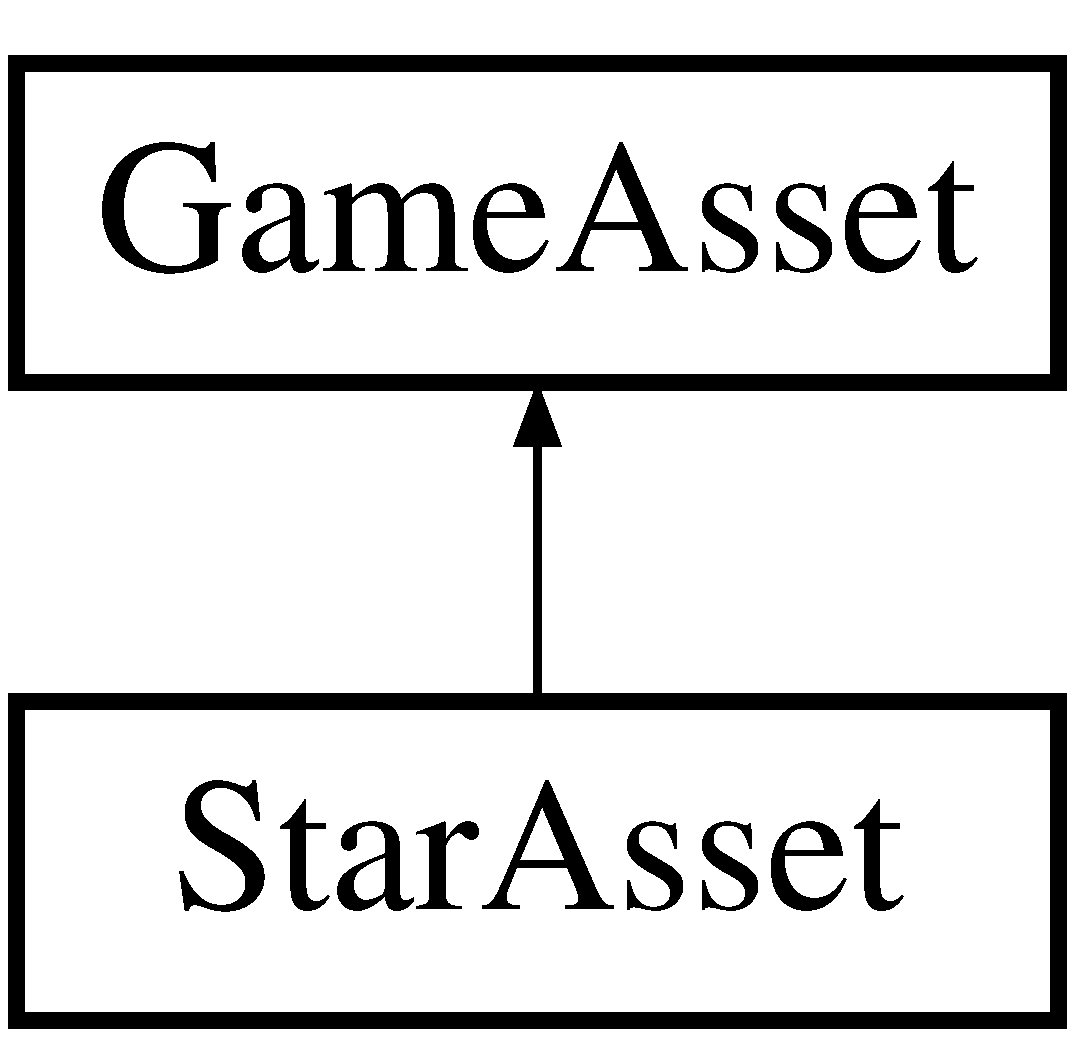
\includegraphics[height=2.000000cm]{classStarAsset}
\end{center}
\end{figure}
\subsection*{Public Types}
\begin{DoxyCompactItemize}
\item 
enum \hyperlink{classStarAsset_a39ac8e905b1e0d2eba0b5c27cd223cef}{vertices} \{ \\*
\hyperlink{classStarAsset_a39ac8e905b1e0d2eba0b5c27cd223cefaadcb919baa5887d4a379bdce37833efe}{F0}, 
\hyperlink{classStarAsset_a39ac8e905b1e0d2eba0b5c27cd223cefa170a4b73924ae45dc9f35aeab6a11ec5}{F1}, 
\hyperlink{classStarAsset_a39ac8e905b1e0d2eba0b5c27cd223cefae935994103227f6914fd7479331c156a}{F2}, 
\hyperlink{classStarAsset_a39ac8e905b1e0d2eba0b5c27cd223cefa0d9d6c5db831f400fb3137b01aaa7f6d}{F3}, 
\\*
\hyperlink{classStarAsset_a39ac8e905b1e0d2eba0b5c27cd223cefa46e1bdb884b4d250c1f826b7e29192d0}{F4}, 
\hyperlink{classStarAsset_a39ac8e905b1e0d2eba0b5c27cd223cefae19e6287a83ee0c27375c0ed1bdf4c1b}{F5}, 
\hyperlink{classStarAsset_a39ac8e905b1e0d2eba0b5c27cd223cefa096f0d517df2f8b60264dedaa3bb8adc}{F6}, 
\hyperlink{classStarAsset_a39ac8e905b1e0d2eba0b5c27cd223cefa59bbf4a0df7d231dfe97e19539da411c}{F7}, 
\\*
\hyperlink{classStarAsset_a39ac8e905b1e0d2eba0b5c27cd223cefaeb5ac468dd02d472c35ca71a96819abe}{F8}, 
\hyperlink{classStarAsset_a39ac8e905b1e0d2eba0b5c27cd223cefafaf00a7281e8c2b6ee7c50a6238fffc2}{F9}, 
\hyperlink{classStarAsset_a39ac8e905b1e0d2eba0b5c27cd223cefae5472cbbc494096850a67cd767b7aebb}{F10}, 
\hyperlink{classStarAsset_a39ac8e905b1e0d2eba0b5c27cd223cefac5eddbc625aca62237c12e905700abc0}{F11}
 \}
\end{DoxyCompactItemize}
\subsection*{Public Member Functions}
\begin{DoxyCompactItemize}
\item 
\hyperlink{classStarAsset_a256d7fef7a77f48eab4af886b2411959}{Star\-Asset} ()
\item 
\hyperlink{classStarAsset_a3dae8c8b498f6029b033aa172f555865}{Star\-Asset} (float x, float y, float z)
\item 
\hyperlink{classStarAsset_a77a07269f87ab84c206d1bc5733e0a10}{$\sim$\-Star\-Asset} ()
\item 
bool \hyperlink{classStarAsset_a359a29db9eaf03058af02bf3bf1d0263}{collides\-With} (\hyperlink{classPlayer}{Player} \&a)
\item 
virtual void \hyperlink{classStarAsset_a21f6e7f632408f34209db35d41f41877}{update} ()
\item 
virtual void \hyperlink{classStarAsset_a0ebfee331ac06d5e58ee0226104ac4e2}{draw} ()
\item 
virtual void \hyperlink{classStarAsset_a0e0f4afbd0edd0d10b7e4a2810222c66}{clean} ()
\end{DoxyCompactItemize}
\subsection*{Additional Inherited Members}


\subsection{Detailed Description}


Definition at line 7 of file Star\-Asset.\-h.



\subsection{Member Enumeration Documentation}
\hypertarget{classStarAsset_a39ac8e905b1e0d2eba0b5c27cd223cef}{\index{Star\-Asset@{Star\-Asset}!vertices@{vertices}}
\index{vertices@{vertices}!StarAsset@{Star\-Asset}}
\subsubsection[{vertices}]{\setlength{\rightskip}{0pt plus 5cm}enum {\bf Star\-Asset\-::vertices}}}\label{classStarAsset_a39ac8e905b1e0d2eba0b5c27cd223cef}
\begin{Desc}
\item[Enumerator]\par
\begin{description}
\index{F0@{F0}!Star\-Asset@{Star\-Asset}}\index{Star\-Asset@{Star\-Asset}!F0@{F0}}\item[{\em 
\hypertarget{classStarAsset_a39ac8e905b1e0d2eba0b5c27cd223cefaadcb919baa5887d4a379bdce37833efe}{F0}\label{classStarAsset_a39ac8e905b1e0d2eba0b5c27cd223cefaadcb919baa5887d4a379bdce37833efe}
}]\index{F1@{F1}!Star\-Asset@{Star\-Asset}}\index{Star\-Asset@{Star\-Asset}!F1@{F1}}\item[{\em 
\hypertarget{classStarAsset_a39ac8e905b1e0d2eba0b5c27cd223cefa170a4b73924ae45dc9f35aeab6a11ec5}{F1}\label{classStarAsset_a39ac8e905b1e0d2eba0b5c27cd223cefa170a4b73924ae45dc9f35aeab6a11ec5}
}]\index{F2@{F2}!Star\-Asset@{Star\-Asset}}\index{Star\-Asset@{Star\-Asset}!F2@{F2}}\item[{\em 
\hypertarget{classStarAsset_a39ac8e905b1e0d2eba0b5c27cd223cefae935994103227f6914fd7479331c156a}{F2}\label{classStarAsset_a39ac8e905b1e0d2eba0b5c27cd223cefae935994103227f6914fd7479331c156a}
}]\index{F3@{F3}!Star\-Asset@{Star\-Asset}}\index{Star\-Asset@{Star\-Asset}!F3@{F3}}\item[{\em 
\hypertarget{classStarAsset_a39ac8e905b1e0d2eba0b5c27cd223cefa0d9d6c5db831f400fb3137b01aaa7f6d}{F3}\label{classStarAsset_a39ac8e905b1e0d2eba0b5c27cd223cefa0d9d6c5db831f400fb3137b01aaa7f6d}
}]\index{F4@{F4}!Star\-Asset@{Star\-Asset}}\index{Star\-Asset@{Star\-Asset}!F4@{F4}}\item[{\em 
\hypertarget{classStarAsset_a39ac8e905b1e0d2eba0b5c27cd223cefa46e1bdb884b4d250c1f826b7e29192d0}{F4}\label{classStarAsset_a39ac8e905b1e0d2eba0b5c27cd223cefa46e1bdb884b4d250c1f826b7e29192d0}
}]\index{F5@{F5}!Star\-Asset@{Star\-Asset}}\index{Star\-Asset@{Star\-Asset}!F5@{F5}}\item[{\em 
\hypertarget{classStarAsset_a39ac8e905b1e0d2eba0b5c27cd223cefae19e6287a83ee0c27375c0ed1bdf4c1b}{F5}\label{classStarAsset_a39ac8e905b1e0d2eba0b5c27cd223cefae19e6287a83ee0c27375c0ed1bdf4c1b}
}]\index{F6@{F6}!Star\-Asset@{Star\-Asset}}\index{Star\-Asset@{Star\-Asset}!F6@{F6}}\item[{\em 
\hypertarget{classStarAsset_a39ac8e905b1e0d2eba0b5c27cd223cefa096f0d517df2f8b60264dedaa3bb8adc}{F6}\label{classStarAsset_a39ac8e905b1e0d2eba0b5c27cd223cefa096f0d517df2f8b60264dedaa3bb8adc}
}]\index{F7@{F7}!Star\-Asset@{Star\-Asset}}\index{Star\-Asset@{Star\-Asset}!F7@{F7}}\item[{\em 
\hypertarget{classStarAsset_a39ac8e905b1e0d2eba0b5c27cd223cefa59bbf4a0df7d231dfe97e19539da411c}{F7}\label{classStarAsset_a39ac8e905b1e0d2eba0b5c27cd223cefa59bbf4a0df7d231dfe97e19539da411c}
}]\index{F8@{F8}!Star\-Asset@{Star\-Asset}}\index{Star\-Asset@{Star\-Asset}!F8@{F8}}\item[{\em 
\hypertarget{classStarAsset_a39ac8e905b1e0d2eba0b5c27cd223cefaeb5ac468dd02d472c35ca71a96819abe}{F8}\label{classStarAsset_a39ac8e905b1e0d2eba0b5c27cd223cefaeb5ac468dd02d472c35ca71a96819abe}
}]\index{F9@{F9}!Star\-Asset@{Star\-Asset}}\index{Star\-Asset@{Star\-Asset}!F9@{F9}}\item[{\em 
\hypertarget{classStarAsset_a39ac8e905b1e0d2eba0b5c27cd223cefafaf00a7281e8c2b6ee7c50a6238fffc2}{F9}\label{classStarAsset_a39ac8e905b1e0d2eba0b5c27cd223cefafaf00a7281e8c2b6ee7c50a6238fffc2}
}]\index{F10@{F10}!Star\-Asset@{Star\-Asset}}\index{Star\-Asset@{Star\-Asset}!F10@{F10}}\item[{\em 
\hypertarget{classStarAsset_a39ac8e905b1e0d2eba0b5c27cd223cefae5472cbbc494096850a67cd767b7aebb}{F10}\label{classStarAsset_a39ac8e905b1e0d2eba0b5c27cd223cefae5472cbbc494096850a67cd767b7aebb}
}]\index{F11@{F11}!Star\-Asset@{Star\-Asset}}\index{Star\-Asset@{Star\-Asset}!F11@{F11}}\item[{\em 
\hypertarget{classStarAsset_a39ac8e905b1e0d2eba0b5c27cd223cefac5eddbc625aca62237c12e905700abc0}{F11}\label{classStarAsset_a39ac8e905b1e0d2eba0b5c27cd223cefac5eddbc625aca62237c12e905700abc0}
}]\end{description}
\end{Desc}


Definition at line 19 of file Star\-Asset.\-h.


\begin{DoxyCode}
19                 \{
20       \hyperlink{classStarAsset_a39ac8e905b1e0d2eba0b5c27cd223cefaadcb919baa5887d4a379bdce37833efe}{F0}, \hyperlink{classStarAsset_a39ac8e905b1e0d2eba0b5c27cd223cefa170a4b73924ae45dc9f35aeab6a11ec5}{F1}, \hyperlink{classStarAsset_a39ac8e905b1e0d2eba0b5c27cd223cefae935994103227f6914fd7479331c156a}{F2}, \hyperlink{classStarAsset_a39ac8e905b1e0d2eba0b5c27cd223cefa0d9d6c5db831f400fb3137b01aaa7f6d}{F3}, \hyperlink{classStarAsset_a39ac8e905b1e0d2eba0b5c27cd223cefa46e1bdb884b4d250c1f826b7e29192d0}{F4}, \hyperlink{classStarAsset_a39ac8e905b1e0d2eba0b5c27cd223cefae19e6287a83ee0c27375c0ed1bdf4c1b}{F5}, \hyperlink{classStarAsset_a39ac8e905b1e0d2eba0b5c27cd223cefa096f0d517df2f8b60264dedaa3bb8adc}{F6}, \hyperlink{classStarAsset_a39ac8e905b1e0d2eba0b5c27cd223cefa59bbf4a0df7d231dfe97e19539da411c}{F7}, \hyperlink{classStarAsset_a39ac8e905b1e0d2eba0b5c27cd223cefaeb5ac468dd02d472c35ca71a96819abe}{F8}, \hyperlink{classStarAsset_a39ac8e905b1e0d2eba0b5c27cd223cefafaf00a7281e8c2b6ee7c50a6238fffc2}{F9}, \hyperlink{classStarAsset_a39ac8e905b1e0d2eba0b5c27cd223cefae5472cbbc494096850a67cd767b7aebb}{F10}, \hyperlink{classStarAsset_a39ac8e905b1e0d2eba0b5c27cd223cefac5eddbc625aca62237c12e905700abc0}{F11}, 
21   \};
\end{DoxyCode}


\subsection{Constructor \& Destructor Documentation}
\hypertarget{classStarAsset_a256d7fef7a77f48eab4af886b2411959}{\index{Star\-Asset@{Star\-Asset}!Star\-Asset@{Star\-Asset}}
\index{Star\-Asset@{Star\-Asset}!StarAsset@{Star\-Asset}}
\subsubsection[{Star\-Asset}]{\setlength{\rightskip}{0pt plus 5cm}Star\-Asset\-::\-Star\-Asset (
\begin{DoxyParamCaption}
{}
\end{DoxyParamCaption}
)}}\label{classStarAsset_a256d7fef7a77f48eab4af886b2411959}


Definition at line 3 of file Star\-Asset.\-cpp.


\begin{DoxyCode}
4   : \hyperlink{classGameAsset_a9c96b0bafa2b6973a2e8c09bf51c52ec}{GameAsset}(
5           \textcolor{keywordtype}{string}(\textcolor{stringliteral}{"CubeRacer/shaders/hello-gl.v.glsl"})
6           , \textcolor{keywordtype}{string}(\textcolor{stringliteral}{"CubeRacer/shaders/starAsset.f.glsl"})
7           )
8 \{
9   \hyperlink{classStarAsset_a256d7fef7a77f48eab4af886b2411959}{StarAsset}(0, 0, 0);
10 \}
\end{DoxyCode}
\hypertarget{classStarAsset_a3dae8c8b498f6029b033aa172f555865}{\index{Star\-Asset@{Star\-Asset}!Star\-Asset@{Star\-Asset}}
\index{Star\-Asset@{Star\-Asset}!StarAsset@{Star\-Asset}}
\subsubsection[{Star\-Asset}]{\setlength{\rightskip}{0pt plus 5cm}Star\-Asset\-::\-Star\-Asset (
\begin{DoxyParamCaption}
\item[{float}]{x, }
\item[{float}]{y, }
\item[{float}]{z}
\end{DoxyParamCaption}
)}}\label{classStarAsset_a3dae8c8b498f6029b033aa172f555865}


Definition at line 12 of file Star\-Asset.\-cpp.


\begin{DoxyCode}
13   : \hyperlink{classGameAsset_a9c96b0bafa2b6973a2e8c09bf51c52ec}{GameAsset}(
14       \textcolor{keywordtype}{string}(\textcolor{stringliteral}{"CubeRacer/shaders/hello-gl.v.glsl"}), 
15       \textcolor{keywordtype}{string}(\textcolor{stringliteral}{"CubeRacer/shaders/starAsset-gl.f.glsl"})
16 )\{
17 
18   \textcolor{comment}{// A default "unit" Star}
19   \hyperlink{classGameAsset_a3e8d7dc58d3d4efafbbce1536b78dbc7}{num\_vertices} = 12;
20   \hyperlink{classGameAsset_aae4d864335c2eca685cc86602881cd18}{num\_triangles} = 20;
21   \hyperlink{classGameAsset_ae1d682ecf84d9cd3f91a8c870acf2777}{g\_vertex\_buffer\_data} = \textcolor{keyword}{new} GLfloat[\hyperlink{classGameAsset_a3e8d7dc58d3d4efafbbce1536b78dbc7}{num\_vertices} * 3]\{
22 
23   \textcolor{comment}{//     x      y     z     //www.clipartbest.com/cliparts/dir/aAp/diraAp9i9.jpeg}
24     -0.65,  -1.0,    0.0,   \textcolor{comment}{//Bottom left point     F0}
25      0.65,  -1.0,    0.0,   \textcolor{comment}{//Bottom right point        F1}
26      0.0,   -0.5,    0.0,   \textcolor{comment}{//Bottom middle point       F2}
27     
28     -0.4,   -0.2,    0.0,   \textcolor{comment}{//Lower-middle left point   F3}
29      0.4,   -0.2,    0.0,   \textcolor{comment}{//Lower-middle right point  F4}
30 
31     -1.0,    0.25,   0.0,   \textcolor{comment}{//Middle left-most point    F5}
32      1.0,    0.25,   0.0,   \textcolor{comment}{//Middle right-most point   F6}
33     -0.25,   0.3,    0.0,   \textcolor{comment}{//Middle left point     F7}
34      0.25,   0.3,    0.0,   \textcolor{comment}{//Middle right point        F8}
35 
36      0.0,    1.0,    0.0,   \textcolor{comment}{//Top point         F9}
37      0.0,    0.0,    0.5,   \textcolor{comment}{//Middle Front point        F10}
38      0.0,    0.0,   -0.5    \textcolor{comment}{//Middle Back point     F11 }
39     
40 \}; \textcolor{comment}{// three points per vertex}
41 
42   \hyperlink{classGameAsset_ab859393c9158c8bda39cd100475fee25}{g\_element\_buffer\_data} = \textcolor{keyword}{new} GLushort[\hyperlink{classGameAsset_aae4d864335c2eca685cc86602881cd18}{num\_triangles} * 3]\{
43 
44     \hyperlink{classStarAsset_a39ac8e905b1e0d2eba0b5c27cd223cefae5472cbbc494096850a67cd767b7aebb}{F10}, \hyperlink{classStarAsset_a39ac8e905b1e0d2eba0b5c27cd223cefa0d9d6c5db831f400fb3137b01aaa7f6d}{F3},  \hyperlink{classStarAsset_a39ac8e905b1e0d2eba0b5c27cd223cefaadcb919baa5887d4a379bdce37833efe}{F0},    \textcolor{comment}{//Bottom left point}
45     \hyperlink{classStarAsset_a39ac8e905b1e0d2eba0b5c27cd223cefaadcb919baa5887d4a379bdce37833efe}{F0},  \hyperlink{classStarAsset_a39ac8e905b1e0d2eba0b5c27cd223cefae935994103227f6914fd7479331c156a}{F2},  \hyperlink{classStarAsset_a39ac8e905b1e0d2eba0b5c27cd223cefae5472cbbc494096850a67cd767b7aebb}{F10},
46 
47     \hyperlink{classStarAsset_a39ac8e905b1e0d2eba0b5c27cd223cefae5472cbbc494096850a67cd767b7aebb}{F10}, \hyperlink{classStarAsset_a39ac8e905b1e0d2eba0b5c27cd223cefae935994103227f6914fd7479331c156a}{F2},  \hyperlink{classStarAsset_a39ac8e905b1e0d2eba0b5c27cd223cefa170a4b73924ae45dc9f35aeab6a11ec5}{F1},    \textcolor{comment}{//Bottom right point}
48     \hyperlink{classStarAsset_a39ac8e905b1e0d2eba0b5c27cd223cefa170a4b73924ae45dc9f35aeab6a11ec5}{F1},  \hyperlink{classStarAsset_a39ac8e905b1e0d2eba0b5c27cd223cefa46e1bdb884b4d250c1f826b7e29192d0}{F4},  \hyperlink{classStarAsset_a39ac8e905b1e0d2eba0b5c27cd223cefae5472cbbc494096850a67cd767b7aebb}{F10},
49 
50     \hyperlink{classStarAsset_a39ac8e905b1e0d2eba0b5c27cd223cefae5472cbbc494096850a67cd767b7aebb}{F10}, \hyperlink{classStarAsset_a39ac8e905b1e0d2eba0b5c27cd223cefa46e1bdb884b4d250c1f826b7e29192d0}{F4},  \hyperlink{classStarAsset_a39ac8e905b1e0d2eba0b5c27cd223cefa096f0d517df2f8b60264dedaa3bb8adc}{F6},    \textcolor{comment}{//Middle right point}
51     \hyperlink{classStarAsset_a39ac8e905b1e0d2eba0b5c27cd223cefa096f0d517df2f8b60264dedaa3bb8adc}{F6},  \hyperlink{classStarAsset_a39ac8e905b1e0d2eba0b5c27cd223cefaeb5ac468dd02d472c35ca71a96819abe}{F8},  \hyperlink{classStarAsset_a39ac8e905b1e0d2eba0b5c27cd223cefae5472cbbc494096850a67cd767b7aebb}{F10},
52     
53     \hyperlink{classStarAsset_a39ac8e905b1e0d2eba0b5c27cd223cefae5472cbbc494096850a67cd767b7aebb}{F10}, \hyperlink{classStarAsset_a39ac8e905b1e0d2eba0b5c27cd223cefaeb5ac468dd02d472c35ca71a96819abe}{F8},  \hyperlink{classStarAsset_a39ac8e905b1e0d2eba0b5c27cd223cefafaf00a7281e8c2b6ee7c50a6238fffc2}{F9},    \textcolor{comment}{//Top point}
54     \hyperlink{classStarAsset_a39ac8e905b1e0d2eba0b5c27cd223cefafaf00a7281e8c2b6ee7c50a6238fffc2}{F9},  \hyperlink{classStarAsset_a39ac8e905b1e0d2eba0b5c27cd223cefa59bbf4a0df7d231dfe97e19539da411c}{F7},  \hyperlink{classStarAsset_a39ac8e905b1e0d2eba0b5c27cd223cefae5472cbbc494096850a67cd767b7aebb}{F10},
55 
56     \hyperlink{classStarAsset_a39ac8e905b1e0d2eba0b5c27cd223cefae5472cbbc494096850a67cd767b7aebb}{F10}, \hyperlink{classStarAsset_a39ac8e905b1e0d2eba0b5c27cd223cefa59bbf4a0df7d231dfe97e19539da411c}{F7},  \hyperlink{classStarAsset_a39ac8e905b1e0d2eba0b5c27cd223cefae19e6287a83ee0c27375c0ed1bdf4c1b}{F5},    \textcolor{comment}{//Middle left point}
57     \hyperlink{classStarAsset_a39ac8e905b1e0d2eba0b5c27cd223cefae19e6287a83ee0c27375c0ed1bdf4c1b}{F5},  \hyperlink{classStarAsset_a39ac8e905b1e0d2eba0b5c27cd223cefa0d9d6c5db831f400fb3137b01aaa7f6d}{F3},  \hyperlink{classStarAsset_a39ac8e905b1e0d2eba0b5c27cd223cefae5472cbbc494096850a67cd767b7aebb}{F10},
58 
59     \hyperlink{classStarAsset_a39ac8e905b1e0d2eba0b5c27cd223cefac5eddbc625aca62237c12e905700abc0}{F11}, \hyperlink{classStarAsset_a39ac8e905b1e0d2eba0b5c27cd223cefa0d9d6c5db831f400fb3137b01aaa7f6d}{F3},  \hyperlink{classStarAsset_a39ac8e905b1e0d2eba0b5c27cd223cefaadcb919baa5887d4a379bdce37833efe}{F0},
60     \hyperlink{classStarAsset_a39ac8e905b1e0d2eba0b5c27cd223cefaadcb919baa5887d4a379bdce37833efe}{F0},  \hyperlink{classStarAsset_a39ac8e905b1e0d2eba0b5c27cd223cefae935994103227f6914fd7479331c156a}{F2},  \hyperlink{classStarAsset_a39ac8e905b1e0d2eba0b5c27cd223cefac5eddbc625aca62237c12e905700abc0}{F11},
61     
62     \hyperlink{classStarAsset_a39ac8e905b1e0d2eba0b5c27cd223cefac5eddbc625aca62237c12e905700abc0}{F11}, \hyperlink{classStarAsset_a39ac8e905b1e0d2eba0b5c27cd223cefae935994103227f6914fd7479331c156a}{F2}, \hyperlink{classStarAsset_a39ac8e905b1e0d2eba0b5c27cd223cefa170a4b73924ae45dc9f35aeab6a11ec5}{F1},
63     \hyperlink{classStarAsset_a39ac8e905b1e0d2eba0b5c27cd223cefa170a4b73924ae45dc9f35aeab6a11ec5}{F1},  \hyperlink{classStarAsset_a39ac8e905b1e0d2eba0b5c27cd223cefa46e1bdb884b4d250c1f826b7e29192d0}{F4}, \hyperlink{classStarAsset_a39ac8e905b1e0d2eba0b5c27cd223cefac5eddbc625aca62237c12e905700abc0}{F11},
64 
65     \hyperlink{classStarAsset_a39ac8e905b1e0d2eba0b5c27cd223cefac5eddbc625aca62237c12e905700abc0}{F11}, \hyperlink{classStarAsset_a39ac8e905b1e0d2eba0b5c27cd223cefa46e1bdb884b4d250c1f826b7e29192d0}{F4}, \hyperlink{classStarAsset_a39ac8e905b1e0d2eba0b5c27cd223cefa096f0d517df2f8b60264dedaa3bb8adc}{F6},
66     \hyperlink{classStarAsset_a39ac8e905b1e0d2eba0b5c27cd223cefa096f0d517df2f8b60264dedaa3bb8adc}{F6},  \hyperlink{classStarAsset_a39ac8e905b1e0d2eba0b5c27cd223cefaeb5ac468dd02d472c35ca71a96819abe}{F8}, \hyperlink{classStarAsset_a39ac8e905b1e0d2eba0b5c27cd223cefac5eddbc625aca62237c12e905700abc0}{F11},
67 
68     \hyperlink{classStarAsset_a39ac8e905b1e0d2eba0b5c27cd223cefac5eddbc625aca62237c12e905700abc0}{F11}, \hyperlink{classStarAsset_a39ac8e905b1e0d2eba0b5c27cd223cefaeb5ac468dd02d472c35ca71a96819abe}{F8}, \hyperlink{classStarAsset_a39ac8e905b1e0d2eba0b5c27cd223cefafaf00a7281e8c2b6ee7c50a6238fffc2}{F9},
69     \hyperlink{classStarAsset_a39ac8e905b1e0d2eba0b5c27cd223cefafaf00a7281e8c2b6ee7c50a6238fffc2}{F9},  \hyperlink{classStarAsset_a39ac8e905b1e0d2eba0b5c27cd223cefa59bbf4a0df7d231dfe97e19539da411c}{F7}, \hyperlink{classStarAsset_a39ac8e905b1e0d2eba0b5c27cd223cefac5eddbc625aca62237c12e905700abc0}{F11},
70 
71     \hyperlink{classStarAsset_a39ac8e905b1e0d2eba0b5c27cd223cefac5eddbc625aca62237c12e905700abc0}{F11}, \hyperlink{classStarAsset_a39ac8e905b1e0d2eba0b5c27cd223cefa59bbf4a0df7d231dfe97e19539da411c}{F7}, \hyperlink{classStarAsset_a39ac8e905b1e0d2eba0b5c27cd223cefae19e6287a83ee0c27375c0ed1bdf4c1b}{F5},
72     \hyperlink{classStarAsset_a39ac8e905b1e0d2eba0b5c27cd223cefa59bbf4a0df7d231dfe97e19539da411c}{F7},  \hyperlink{classStarAsset_a39ac8e905b1e0d2eba0b5c27cd223cefa0d9d6c5db831f400fb3137b01aaa7f6d}{F3}, F11    
73 
74 \}; \textcolor{comment}{// three vertices per triangle}
75 
76   \hyperlink{classGameAsset_a3444a096fed505b1740bedc95e2cfa6c}{bbox}.reset();
77   \hyperlink{classGameAsset_a3444a096fed505b1740bedc95e2cfa6c}{bbox} = shared\_ptr<BoundingBox>(\textcolor{keyword}{new} \hyperlink{classBoundingBox}{BoundingBox}(\hyperlink{classVectormath_1_1Aos_1_1Point3}{Point3}(x, y, z), 1.0, 1.0, 1.0));
78 
79   \hyperlink{classGameAsset_aa26d85233ece476d599adf90074e9568}{make\_resources}();
80 \}
\end{DoxyCode}
\hypertarget{classStarAsset_a77a07269f87ab84c206d1bc5733e0a10}{\index{Star\-Asset@{Star\-Asset}!$\sim$\-Star\-Asset@{$\sim$\-Star\-Asset}}
\index{$\sim$\-Star\-Asset@{$\sim$\-Star\-Asset}!StarAsset@{Star\-Asset}}
\subsubsection[{$\sim$\-Star\-Asset}]{\setlength{\rightskip}{0pt plus 5cm}Star\-Asset\-::$\sim$\-Star\-Asset (
\begin{DoxyParamCaption}
{}
\end{DoxyParamCaption}
)}}\label{classStarAsset_a77a07269f87ab84c206d1bc5733e0a10}


Definition at line 82 of file Star\-Asset.\-cpp.


\begin{DoxyCode}
82                       \{
83   \textcolor{comment}{// TODO: do something nice and fun here.}
84 \}
\end{DoxyCode}


\subsection{Member Function Documentation}
\hypertarget{classStarAsset_a0e0f4afbd0edd0d10b7e4a2810222c66}{\index{Star\-Asset@{Star\-Asset}!clean@{clean}}
\index{clean@{clean}!StarAsset@{Star\-Asset}}
\subsubsection[{clean}]{\setlength{\rightskip}{0pt plus 5cm}void Star\-Asset\-::clean (
\begin{DoxyParamCaption}
{}
\end{DoxyParamCaption}
)\hspace{0.3cm}{\ttfamily [virtual]}}}\label{classStarAsset_a0e0f4afbd0edd0d10b7e4a2810222c66}


Implements \hyperlink{classGameAsset_abbea962eaa63a813949b834778b7483e}{Game\-Asset}.



Definition at line 104 of file Star\-Asset.\-cpp.


\begin{DoxyCode}
104 \{ \} 
\end{DoxyCode}
\hypertarget{classStarAsset_a359a29db9eaf03058af02bf3bf1d0263}{\index{Star\-Asset@{Star\-Asset}!collides\-With@{collides\-With}}
\index{collides\-With@{collides\-With}!StarAsset@{Star\-Asset}}
\subsubsection[{collides\-With}]{\setlength{\rightskip}{0pt plus 5cm}bool Star\-Asset\-::collides\-With (
\begin{DoxyParamCaption}
\item[{{\bf Player} \&}]{a}
\end{DoxyParamCaption}
)}}\label{classStarAsset_a359a29db9eaf03058af02bf3bf1d0263}


Definition at line 96 of file Star\-Asset.\-cpp.


\begin{DoxyCode}
96                                        \{
97   \textcolor{keywordflow}{return} \hyperlink{classGameAsset_a3444a096fed505b1740bedc95e2cfa6c}{bbox}->collidesWith((*a.\hyperlink{classGameAsset_a3444a096fed505b1740bedc95e2cfa6c}{bbox}));
98 \}
\end{DoxyCode}
\hypertarget{classStarAsset_a0ebfee331ac06d5e58ee0226104ac4e2}{\index{Star\-Asset@{Star\-Asset}!draw@{draw}}
\index{draw@{draw}!StarAsset@{Star\-Asset}}
\subsubsection[{draw}]{\setlength{\rightskip}{0pt plus 5cm}void Star\-Asset\-::draw (
\begin{DoxyParamCaption}
{}
\end{DoxyParamCaption}
)\hspace{0.3cm}{\ttfamily [virtual]}}}\label{classStarAsset_a0ebfee331ac06d5e58ee0226104ac4e2}


Reimplemented from \hyperlink{classGameAsset_a2d7e18a8f1dd8ba89ed1bd14f2affeab}{Game\-Asset}.



Definition at line 100 of file Star\-Asset.\-cpp.


\begin{DoxyCode}
100                      \{
101   \hyperlink{classGameAsset_a2d7e18a8f1dd8ba89ed1bd14f2affeab}{GameAsset::draw}();
102 \}
\end{DoxyCode}
\hypertarget{classStarAsset_a21f6e7f632408f34209db35d41f41877}{\index{Star\-Asset@{Star\-Asset}!update@{update}}
\index{update@{update}!StarAsset@{Star\-Asset}}
\subsubsection[{update}]{\setlength{\rightskip}{0pt plus 5cm}void Star\-Asset\-::update (
\begin{DoxyParamCaption}
{}
\end{DoxyParamCaption}
)\hspace{0.3cm}{\ttfamily [virtual]}}}\label{classStarAsset_a21f6e7f632408f34209db35d41f41877}


Implements \hyperlink{classGameAsset_a42688ec8f02e201eaaa01e74a112083f}{Game\-Asset}.



Definition at line 86 of file Star\-Asset.\-cpp.


\begin{DoxyCode}
86                        \{
87   \textcolor{keywordflow}{if} (\hyperlink{classGameAsset_aebf93ae52dc7fabbb6ec7edaadf915d0}{isAlive}) \{
88     shared\_ptr<Point3> p = shared\_ptr<Point3>(\textcolor{keyword}{new} \hyperlink{classVectormath_1_1Aos_1_1Point3}{Point3}(this->\hyperlink{classGameAsset_a3444a096fed505b1740bedc95e2cfa6c}{bbox}->getCentre()->getX(), -0.3, 
      this->\hyperlink{classGameAsset_a3444a096fed505b1740bedc95e2cfa6c}{bbox}->getCentre()->getZ()-0.2));
89 
90     \hyperlink{classGameAsset_a3444a096fed505b1740bedc95e2cfa6c}{bbox}.reset();
91     \hyperlink{classGameAsset_a3444a096fed505b1740bedc95e2cfa6c}{bbox} = shared\_ptr<BoundingBox>(\textcolor{keyword}{new} \hyperlink{classBoundingBox}{BoundingBox}(*p, 1.0, 1.0, 1.0));
92     \textcolor{keywordflow}{if}( this->\hyperlink{classGameAsset_a3444a096fed505b1740bedc95e2cfa6c}{bbox}->getCentre()->getZ() < -5) \{ this->\hyperlink{classGameAsset_a631982e6d36061c08c7e8981ce0fd308}{dead}(); \}
93   \}
94 \}
\end{DoxyCode}


The documentation for this class was generated from the following files\-:\begin{DoxyCompactItemize}
\item 
/home/sam/\-Cube\-Racer/src/\hyperlink{StarAsset_8h}{Star\-Asset.\-h}\item 
/home/sam/\-Cube\-Racer/src/\hyperlink{StarAsset_8cpp}{Star\-Asset.\-cpp}\end{DoxyCompactItemize}

\hypertarget{classVectormath_1_1Aos_1_1Transform3}{\section{Vectormath\-:\-:Aos\-:\-:Transform3 Class Reference}
\label{classVectormath_1_1Aos_1_1Transform3}\index{Vectormath\-::\-Aos\-::\-Transform3@{Vectormath\-::\-Aos\-::\-Transform3}}
}


{\ttfamily \#include $<$vectormath\-\_\-aos.\-h$>$}

\subsection*{Public Member Functions}
\begin{DoxyCompactItemize}
\item 
\hyperlink{classVectormath_1_1Aos_1_1Transform3_a4c361ee4538c41a3d4dacc50b428b2ba}{Transform3} ()
\item 
\hyperlink{classVectormath_1_1Aos_1_1Transform3_a77ffda55c385ce413eb6f393485cc168}{Transform3} (const \hyperlink{classVectormath_1_1Aos_1_1Transform3}{Transform3} \&tfrm)
\item 
\hyperlink{classVectormath_1_1Aos_1_1Transform3_a43872d7a822d5384e3ee631d035d91be}{Transform3} (const \hyperlink{classVectormath_1_1Aos_1_1Vector3}{Vector3} \&col0, const \hyperlink{classVectormath_1_1Aos_1_1Vector3}{Vector3} \&col1, const \hyperlink{classVectormath_1_1Aos_1_1Vector3}{Vector3} \&col2, const \hyperlink{classVectormath_1_1Aos_1_1Vector3}{Vector3} \&col3)
\item 
\hyperlink{classVectormath_1_1Aos_1_1Transform3_a2c98e657db82e24e18c96a8a08f7cf74}{Transform3} (const \hyperlink{classVectormath_1_1Aos_1_1Matrix3}{Matrix3} \&tfrm, const \hyperlink{classVectormath_1_1Aos_1_1Vector3}{Vector3} \&translate\-Vec)
\item 
\hyperlink{classVectormath_1_1Aos_1_1Transform3_a5a2129a250b2482d68f5c366d9d67b59}{Transform3} (const \hyperlink{classVectormath_1_1Aos_1_1Quat}{Quat} \&unit\-Quat, const \hyperlink{classVectormath_1_1Aos_1_1Vector3}{Vector3} \&translate\-Vec)
\item 
\hyperlink{classVectormath_1_1Aos_1_1Transform3_afa3e8f627015d6c105f49b9cc993d980}{Transform3} (float scalar)
\item 
\hyperlink{classVectormath_1_1Aos_1_1Transform3}{Transform3} \& \hyperlink{classVectormath_1_1Aos_1_1Transform3_ad25d63812cd76766720009970c8c80bc}{operator=} (const \hyperlink{classVectormath_1_1Aos_1_1Transform3}{Transform3} \&tfrm)
\item 
\hyperlink{classVectormath_1_1Aos_1_1Transform3}{Transform3} \& \hyperlink{classVectormath_1_1Aos_1_1Transform3_abe5cd8955f4333ebe26b29b2cd675399}{set\-Upper3x3} (const \hyperlink{classVectormath_1_1Aos_1_1Matrix3}{Matrix3} \&mat3)
\item 
const \hyperlink{classVectormath_1_1Aos_1_1Matrix3}{Matrix3} \hyperlink{classVectormath_1_1Aos_1_1Transform3_a06797b4731acac19f070b886253b435b}{get\-Upper3x3} () const 
\item 
\hyperlink{classVectormath_1_1Aos_1_1Transform3}{Transform3} \& \hyperlink{classVectormath_1_1Aos_1_1Transform3_a6c55ac4d2ffea34ef6aa5d3dea3768ce}{set\-Translation} (const \hyperlink{classVectormath_1_1Aos_1_1Vector3}{Vector3} \&translate\-Vec)
\item 
const \hyperlink{classVectormath_1_1Aos_1_1Vector3}{Vector3} \hyperlink{classVectormath_1_1Aos_1_1Transform3_ab4fbda61a2b91bb826066bf384a94cd0}{get\-Translation} () const 
\item 
\hyperlink{classVectormath_1_1Aos_1_1Transform3}{Transform3} \& \hyperlink{classVectormath_1_1Aos_1_1Transform3_a379d1863457b97607424c7d7036bf1eb}{set\-Col0} (const \hyperlink{classVectormath_1_1Aos_1_1Vector3}{Vector3} \&col0)
\item 
\hyperlink{classVectormath_1_1Aos_1_1Transform3}{Transform3} \& \hyperlink{classVectormath_1_1Aos_1_1Transform3_a974966028c02f19ad2c63fa182153b30}{set\-Col1} (const \hyperlink{classVectormath_1_1Aos_1_1Vector3}{Vector3} \&col1)
\item 
\hyperlink{classVectormath_1_1Aos_1_1Transform3}{Transform3} \& \hyperlink{classVectormath_1_1Aos_1_1Transform3_a8d9bd044ef5de78704566cf12a0fd9a6}{set\-Col2} (const \hyperlink{classVectormath_1_1Aos_1_1Vector3}{Vector3} \&col2)
\item 
\hyperlink{classVectormath_1_1Aos_1_1Transform3}{Transform3} \& \hyperlink{classVectormath_1_1Aos_1_1Transform3_a4bbefd547e301601b7f6c37371509952}{set\-Col3} (const \hyperlink{classVectormath_1_1Aos_1_1Vector3}{Vector3} \&col3)
\item 
const \hyperlink{classVectormath_1_1Aos_1_1Vector3}{Vector3} \hyperlink{classVectormath_1_1Aos_1_1Transform3_af0beb2dbbc0c9b21c50c092c7a00219d}{get\-Col0} () const 
\item 
const \hyperlink{classVectormath_1_1Aos_1_1Vector3}{Vector3} \hyperlink{classVectormath_1_1Aos_1_1Transform3_a599e8e829f4da3ca98f5e6ec37bc245a}{get\-Col1} () const 
\item 
const \hyperlink{classVectormath_1_1Aos_1_1Vector3}{Vector3} \hyperlink{classVectormath_1_1Aos_1_1Transform3_a2456a9c9a3928065c156d327fca3bfcd}{get\-Col2} () const 
\item 
const \hyperlink{classVectormath_1_1Aos_1_1Vector3}{Vector3} \hyperlink{classVectormath_1_1Aos_1_1Transform3_a06e3160b31b82a325a0a204082bc4720}{get\-Col3} () const 
\item 
\hyperlink{classVectormath_1_1Aos_1_1Transform3}{Transform3} \& \hyperlink{classVectormath_1_1Aos_1_1Transform3_a0a4ba5d1dbbdb94b14efacc20897d001}{set\-Col} (int col, const \hyperlink{classVectormath_1_1Aos_1_1Vector3}{Vector3} \&vec)
\item 
\hyperlink{classVectormath_1_1Aos_1_1Transform3}{Transform3} \& \hyperlink{classVectormath_1_1Aos_1_1Transform3_a0bc58cd41ab7c52cda6f86e1780d1ad4}{set\-Row} (int row, const \hyperlink{classVectormath_1_1Aos_1_1Vector4}{Vector4} \&vec)
\item 
const \hyperlink{classVectormath_1_1Aos_1_1Vector3}{Vector3} \hyperlink{classVectormath_1_1Aos_1_1Transform3_a6c04fe588c10315223cb2583618b260e}{get\-Col} (int col) const 
\item 
const \hyperlink{classVectormath_1_1Aos_1_1Vector4}{Vector4} \hyperlink{classVectormath_1_1Aos_1_1Transform3_ac38d9f289e1d523c7aaeb980d31532a6}{get\-Row} (int row) const 
\item 
\hyperlink{classVectormath_1_1Aos_1_1Vector3}{Vector3} \& \hyperlink{classVectormath_1_1Aos_1_1Transform3_ae72712700374ed276af6e06f2eae50a1}{operator\mbox{[}$\,$\mbox{]}} (int col)
\item 
const \hyperlink{classVectormath_1_1Aos_1_1Vector3}{Vector3} \hyperlink{classVectormath_1_1Aos_1_1Transform3_a8dcf15dbc045d038e3fe11c1eaf8f9cb}{operator\mbox{[}$\,$\mbox{]}} (int col) const 
\item 
\hyperlink{classVectormath_1_1Aos_1_1Transform3}{Transform3} \& \hyperlink{classVectormath_1_1Aos_1_1Transform3_ab8d7007317ffc2ef1d0bdf838acfce36}{set\-Elem} (int col, int row, float val)
\item 
float \hyperlink{classVectormath_1_1Aos_1_1Transform3_aa351e32f7c872626e71e1554a6489f36}{get\-Elem} (int col, int row) const 
\item 
const \hyperlink{classVectormath_1_1Aos_1_1Vector3}{Vector3} \hyperlink{classVectormath_1_1Aos_1_1Transform3_a02d3e76a76eca287c89e6d725661dc9b}{operator$\ast$} (const \hyperlink{classVectormath_1_1Aos_1_1Vector3}{Vector3} \&vec) const 
\item 
const \hyperlink{classVectormath_1_1Aos_1_1Point3}{Point3} \hyperlink{classVectormath_1_1Aos_1_1Transform3_afb24b2eb78a98ab5afeb4202976f3f6f}{operator$\ast$} (const \hyperlink{classVectormath_1_1Aos_1_1Point3}{Point3} \&pnt) const 
\item 
const \hyperlink{classVectormath_1_1Aos_1_1Transform3}{Transform3} \hyperlink{classVectormath_1_1Aos_1_1Transform3_aaafd7e1c85d3fa3c7aa12563fe0ccd18}{operator$\ast$} (const \hyperlink{classVectormath_1_1Aos_1_1Transform3}{Transform3} \&tfrm) const 
\item 
\hyperlink{classVectormath_1_1Aos_1_1Transform3}{Transform3} \& \hyperlink{classVectormath_1_1Aos_1_1Transform3_a0a02f0eca1169fb4d127e21ff0fa4854}{operator$\ast$=} (const \hyperlink{classVectormath_1_1Aos_1_1Transform3}{Transform3} \&tfrm)
\end{DoxyCompactItemize}
\subsection*{Static Public Member Functions}
\begin{DoxyCompactItemize}
\item 
static const \hyperlink{classVectormath_1_1Aos_1_1Transform3}{Transform3} \hyperlink{classVectormath_1_1Aos_1_1Transform3_a206174e7a6c82fcd3a3be3c2eaa1c4c8}{identity} ()
\item 
static const \hyperlink{classVectormath_1_1Aos_1_1Transform3}{Transform3} \hyperlink{classVectormath_1_1Aos_1_1Transform3_a0789b73803fc9af8a408728026ea1547}{rotation\-X} (float radians)
\item 
static const \hyperlink{classVectormath_1_1Aos_1_1Transform3}{Transform3} \hyperlink{classVectormath_1_1Aos_1_1Transform3_ad8adbbcbbcfb9000f9f71d39e51f9422}{rotation\-Y} (float radians)
\item 
static const \hyperlink{classVectormath_1_1Aos_1_1Transform3}{Transform3} \hyperlink{classVectormath_1_1Aos_1_1Transform3_a88063872802cd561b7c692784b8c0341}{rotation\-Z} (float radians)
\item 
static const \hyperlink{classVectormath_1_1Aos_1_1Transform3}{Transform3} \hyperlink{classVectormath_1_1Aos_1_1Transform3_aee405eb7dc13075bbeac943259aa950d}{rotation\-Z\-Y\-X} (const \hyperlink{classVectormath_1_1Aos_1_1Vector3}{Vector3} \&radians\-X\-Y\-Z)
\item 
static const \hyperlink{classVectormath_1_1Aos_1_1Transform3}{Transform3} \hyperlink{classVectormath_1_1Aos_1_1Transform3_a56e3588c1c10d375515d00e4479369a7}{rotation} (float radians, const \hyperlink{classVectormath_1_1Aos_1_1Vector3}{Vector3} \&unit\-Vec)
\item 
static const \hyperlink{classVectormath_1_1Aos_1_1Transform3}{Transform3} \hyperlink{classVectormath_1_1Aos_1_1Transform3_afdcea7a2ac0c81a95c3e3bacecd635ad}{rotation} (const \hyperlink{classVectormath_1_1Aos_1_1Quat}{Quat} \&unit\-Quat)
\item 
static const \hyperlink{classVectormath_1_1Aos_1_1Transform3}{Transform3} \hyperlink{classVectormath_1_1Aos_1_1Transform3_a3a85d536b4e3a335d75a1e5cef98f0f5}{scale} (const \hyperlink{classVectormath_1_1Aos_1_1Vector3}{Vector3} \&scale\-Vec)
\item 
static const \hyperlink{classVectormath_1_1Aos_1_1Transform3}{Transform3} \hyperlink{classVectormath_1_1Aos_1_1Transform3_aae2d74bd8a2609917fdfc6fd8913413c}{translation} (const \hyperlink{classVectormath_1_1Aos_1_1Vector3}{Vector3} \&translate\-Vec)
\end{DoxyCompactItemize}


\subsection{Detailed Description}


Definition at line 1657 of file vectormath\-\_\-aos.\-h.



\subsection{Constructor \& Destructor Documentation}
\hypertarget{classVectormath_1_1Aos_1_1Transform3_a4c361ee4538c41a3d4dacc50b428b2ba}{\index{Vectormath\-::\-Aos\-::\-Transform3@{Vectormath\-::\-Aos\-::\-Transform3}!Transform3@{Transform3}}
\index{Transform3@{Transform3}!Vectormath::Aos::Transform3@{Vectormath\-::\-Aos\-::\-Transform3}}
\subsubsection[{Transform3}]{\setlength{\rightskip}{0pt plus 5cm}Vectormath\-::\-Aos\-::\-Transform3\-::\-Transform3 (
\begin{DoxyParamCaption}
{}
\end{DoxyParamCaption}
)\hspace{0.3cm}{\ttfamily [inline]}}}\label{classVectormath_1_1Aos_1_1Transform3_a4c361ee4538c41a3d4dacc50b428b2ba}


Definition at line 1667 of file vectormath\-\_\-aos.\-h.


\begin{DoxyCode}
1667 \{ \};
\end{DoxyCode}
\hypertarget{classVectormath_1_1Aos_1_1Transform3_a77ffda55c385ce413eb6f393485cc168}{\index{Vectormath\-::\-Aos\-::\-Transform3@{Vectormath\-::\-Aos\-::\-Transform3}!Transform3@{Transform3}}
\index{Transform3@{Transform3}!Vectormath::Aos::Transform3@{Vectormath\-::\-Aos\-::\-Transform3}}
\subsubsection[{Transform3}]{\setlength{\rightskip}{0pt plus 5cm}Vectormath\-::\-Aos\-::\-Transform3\-::\-Transform3 (
\begin{DoxyParamCaption}
\item[{const {\bf Transform3} \&}]{tfrm}
\end{DoxyParamCaption}
)\hspace{0.3cm}{\ttfamily [inline]}}}\label{classVectormath_1_1Aos_1_1Transform3_a77ffda55c385ce413eb6f393485cc168}


Definition at line 1127 of file mat\-\_\-aos.\-h.


\begin{DoxyCode}
1128 \{
1129     mCol0 = tfrm.mCol0;
1130     mCol1 = tfrm.mCol1;
1131     mCol2 = tfrm.mCol2;
1132     mCol3 = tfrm.mCol3;
1133 \}
\end{DoxyCode}
\hypertarget{classVectormath_1_1Aos_1_1Transform3_a43872d7a822d5384e3ee631d035d91be}{\index{Vectormath\-::\-Aos\-::\-Transform3@{Vectormath\-::\-Aos\-::\-Transform3}!Transform3@{Transform3}}
\index{Transform3@{Transform3}!Vectormath::Aos::Transform3@{Vectormath\-::\-Aos\-::\-Transform3}}
\subsubsection[{Transform3}]{\setlength{\rightskip}{0pt plus 5cm}Vectormath\-::\-Aos\-::\-Transform3\-::\-Transform3 (
\begin{DoxyParamCaption}
\item[{const {\bf Vector3} \&}]{col0, }
\item[{const {\bf Vector3} \&}]{col1, }
\item[{const {\bf Vector3} \&}]{col2, }
\item[{const {\bf Vector3} \&}]{col3}
\end{DoxyParamCaption}
)\hspace{0.3cm}{\ttfamily [inline]}}}\label{classVectormath_1_1Aos_1_1Transform3_a43872d7a822d5384e3ee631d035d91be}


Definition at line 1143 of file mat\-\_\-aos.\-h.


\begin{DoxyCode}
1144 \{
1145     mCol0 = \_col0;
1146     mCol1 = \_col1;
1147     mCol2 = \_col2;
1148     mCol3 = \_col3;
1149 \}
\end{DoxyCode}
\hypertarget{classVectormath_1_1Aos_1_1Transform3_a2c98e657db82e24e18c96a8a08f7cf74}{\index{Vectormath\-::\-Aos\-::\-Transform3@{Vectormath\-::\-Aos\-::\-Transform3}!Transform3@{Transform3}}
\index{Transform3@{Transform3}!Vectormath::Aos::Transform3@{Vectormath\-::\-Aos\-::\-Transform3}}
\subsubsection[{Transform3}]{\setlength{\rightskip}{0pt plus 5cm}Vectormath\-::\-Aos\-::\-Transform3\-::\-Transform3 (
\begin{DoxyParamCaption}
\item[{const {\bf Matrix3} \&}]{tfrm, }
\item[{const {\bf Vector3} \&}]{translate\-Vec}
\end{DoxyParamCaption}
)\hspace{0.3cm}{\ttfamily [inline]}}}\label{classVectormath_1_1Aos_1_1Transform3_a2c98e657db82e24e18c96a8a08f7cf74}


Definition at line 1151 of file mat\-\_\-aos.\-h.


\begin{DoxyCode}
1152 \{
1153     this->\hyperlink{classVectormath_1_1Aos_1_1Transform3_abe5cd8955f4333ebe26b29b2cd675399}{setUpper3x3}( tfrm );
1154     this->\hyperlink{classVectormath_1_1Aos_1_1Transform3_a6c55ac4d2ffea34ef6aa5d3dea3768ce}{setTranslation}( translateVec );
1155 \}
\end{DoxyCode}
\hypertarget{classVectormath_1_1Aos_1_1Transform3_a5a2129a250b2482d68f5c366d9d67b59}{\index{Vectormath\-::\-Aos\-::\-Transform3@{Vectormath\-::\-Aos\-::\-Transform3}!Transform3@{Transform3}}
\index{Transform3@{Transform3}!Vectormath::Aos::Transform3@{Vectormath\-::\-Aos\-::\-Transform3}}
\subsubsection[{Transform3}]{\setlength{\rightskip}{0pt plus 5cm}Vectormath\-::\-Aos\-::\-Transform3\-::\-Transform3 (
\begin{DoxyParamCaption}
\item[{const {\bf Quat} \&}]{unit\-Quat, }
\item[{const {\bf Vector3} \&}]{translate\-Vec}
\end{DoxyParamCaption}
)\hspace{0.3cm}{\ttfamily [inline]}}}\label{classVectormath_1_1Aos_1_1Transform3_a5a2129a250b2482d68f5c366d9d67b59}


Definition at line 1157 of file mat\-\_\-aos.\-h.


\begin{DoxyCode}
1158 \{
1159     this->\hyperlink{classVectormath_1_1Aos_1_1Transform3_abe5cd8955f4333ebe26b29b2cd675399}{setUpper3x3}( Matrix3( unitQuat ) );
1160     this->\hyperlink{classVectormath_1_1Aos_1_1Transform3_a6c55ac4d2ffea34ef6aa5d3dea3768ce}{setTranslation}( translateVec );
1161 \}
\end{DoxyCode}
\hypertarget{classVectormath_1_1Aos_1_1Transform3_afa3e8f627015d6c105f49b9cc993d980}{\index{Vectormath\-::\-Aos\-::\-Transform3@{Vectormath\-::\-Aos\-::\-Transform3}!Transform3@{Transform3}}
\index{Transform3@{Transform3}!Vectormath::Aos::Transform3@{Vectormath\-::\-Aos\-::\-Transform3}}
\subsubsection[{Transform3}]{\setlength{\rightskip}{0pt plus 5cm}Vectormath\-::\-Aos\-::\-Transform3\-::\-Transform3 (
\begin{DoxyParamCaption}
\item[{float}]{scalar}
\end{DoxyParamCaption}
)\hspace{0.3cm}{\ttfamily [inline]}, {\ttfamily [explicit]}}}\label{classVectormath_1_1Aos_1_1Transform3_afa3e8f627015d6c105f49b9cc993d980}


Definition at line 1135 of file mat\-\_\-aos.\-h.


\begin{DoxyCode}
1136 \{
1137     mCol0 = Vector3( scalar );
1138     mCol1 = Vector3( scalar );
1139     mCol2 = Vector3( scalar );
1140     mCol3 = Vector3( scalar );
1141 \}
\end{DoxyCode}


\subsection{Member Function Documentation}
\hypertarget{classVectormath_1_1Aos_1_1Transform3_a6c04fe588c10315223cb2583618b260e}{\index{Vectormath\-::\-Aos\-::\-Transform3@{Vectormath\-::\-Aos\-::\-Transform3}!get\-Col@{get\-Col}}
\index{get\-Col@{get\-Col}!Vectormath::Aos::Transform3@{Vectormath\-::\-Aos\-::\-Transform3}}
\subsubsection[{get\-Col}]{\setlength{\rightskip}{0pt plus 5cm}const {\bf Vector3} Vectormath\-::\-Aos\-::\-Transform3\-::get\-Col (
\begin{DoxyParamCaption}
\item[{int}]{col}
\end{DoxyParamCaption}
) const\hspace{0.3cm}{\ttfamily [inline]}}}\label{classVectormath_1_1Aos_1_1Transform3_a6c04fe588c10315223cb2583618b260e}


Definition at line 1236 of file mat\-\_\-aos.\-h.


\begin{DoxyCode}
1237 \{
1238     \textcolor{keywordflow}{return} *(&mCol0 + col);
1239 \}
\end{DoxyCode}
\hypertarget{classVectormath_1_1Aos_1_1Transform3_af0beb2dbbc0c9b21c50c092c7a00219d}{\index{Vectormath\-::\-Aos\-::\-Transform3@{Vectormath\-::\-Aos\-::\-Transform3}!get\-Col0@{get\-Col0}}
\index{get\-Col0@{get\-Col0}!Vectormath::Aos::Transform3@{Vectormath\-::\-Aos\-::\-Transform3}}
\subsubsection[{get\-Col0}]{\setlength{\rightskip}{0pt plus 5cm}const {\bf Vector3} Vectormath\-::\-Aos\-::\-Transform3\-::get\-Col0 (
\begin{DoxyParamCaption}
{}
\end{DoxyParamCaption}
) const\hspace{0.3cm}{\ttfamily [inline]}}}\label{classVectormath_1_1Aos_1_1Transform3_af0beb2dbbc0c9b21c50c092c7a00219d}


Definition at line 1216 of file mat\-\_\-aos.\-h.


\begin{DoxyCode}
1217 \{
1218     \textcolor{keywordflow}{return} mCol0;
1219 \}
\end{DoxyCode}
\hypertarget{classVectormath_1_1Aos_1_1Transform3_a599e8e829f4da3ca98f5e6ec37bc245a}{\index{Vectormath\-::\-Aos\-::\-Transform3@{Vectormath\-::\-Aos\-::\-Transform3}!get\-Col1@{get\-Col1}}
\index{get\-Col1@{get\-Col1}!Vectormath::Aos::Transform3@{Vectormath\-::\-Aos\-::\-Transform3}}
\subsubsection[{get\-Col1}]{\setlength{\rightskip}{0pt plus 5cm}const {\bf Vector3} Vectormath\-::\-Aos\-::\-Transform3\-::get\-Col1 (
\begin{DoxyParamCaption}
{}
\end{DoxyParamCaption}
) const\hspace{0.3cm}{\ttfamily [inline]}}}\label{classVectormath_1_1Aos_1_1Transform3_a599e8e829f4da3ca98f5e6ec37bc245a}


Definition at line 1221 of file mat\-\_\-aos.\-h.


\begin{DoxyCode}
1222 \{
1223     \textcolor{keywordflow}{return} mCol1;
1224 \}
\end{DoxyCode}
\hypertarget{classVectormath_1_1Aos_1_1Transform3_a2456a9c9a3928065c156d327fca3bfcd}{\index{Vectormath\-::\-Aos\-::\-Transform3@{Vectormath\-::\-Aos\-::\-Transform3}!get\-Col2@{get\-Col2}}
\index{get\-Col2@{get\-Col2}!Vectormath::Aos::Transform3@{Vectormath\-::\-Aos\-::\-Transform3}}
\subsubsection[{get\-Col2}]{\setlength{\rightskip}{0pt plus 5cm}const {\bf Vector3} Vectormath\-::\-Aos\-::\-Transform3\-::get\-Col2 (
\begin{DoxyParamCaption}
{}
\end{DoxyParamCaption}
) const\hspace{0.3cm}{\ttfamily [inline]}}}\label{classVectormath_1_1Aos_1_1Transform3_a2456a9c9a3928065c156d327fca3bfcd}


Definition at line 1226 of file mat\-\_\-aos.\-h.


\begin{DoxyCode}
1227 \{
1228     \textcolor{keywordflow}{return} mCol2;
1229 \}
\end{DoxyCode}
\hypertarget{classVectormath_1_1Aos_1_1Transform3_a06e3160b31b82a325a0a204082bc4720}{\index{Vectormath\-::\-Aos\-::\-Transform3@{Vectormath\-::\-Aos\-::\-Transform3}!get\-Col3@{get\-Col3}}
\index{get\-Col3@{get\-Col3}!Vectormath::Aos::Transform3@{Vectormath\-::\-Aos\-::\-Transform3}}
\subsubsection[{get\-Col3}]{\setlength{\rightskip}{0pt plus 5cm}const {\bf Vector3} Vectormath\-::\-Aos\-::\-Transform3\-::get\-Col3 (
\begin{DoxyParamCaption}
{}
\end{DoxyParamCaption}
) const\hspace{0.3cm}{\ttfamily [inline]}}}\label{classVectormath_1_1Aos_1_1Transform3_a06e3160b31b82a325a0a204082bc4720}


Definition at line 1231 of file mat\-\_\-aos.\-h.


\begin{DoxyCode}
1232 \{
1233     \textcolor{keywordflow}{return} mCol3;
1234 \}
\end{DoxyCode}
\hypertarget{classVectormath_1_1Aos_1_1Transform3_aa351e32f7c872626e71e1554a6489f36}{\index{Vectormath\-::\-Aos\-::\-Transform3@{Vectormath\-::\-Aos\-::\-Transform3}!get\-Elem@{get\-Elem}}
\index{get\-Elem@{get\-Elem}!Vectormath::Aos::Transform3@{Vectormath\-::\-Aos\-::\-Transform3}}
\subsubsection[{get\-Elem}]{\setlength{\rightskip}{0pt plus 5cm}float Vectormath\-::\-Aos\-::\-Transform3\-::get\-Elem (
\begin{DoxyParamCaption}
\item[{int}]{col, }
\item[{int}]{row}
\end{DoxyParamCaption}
) const\hspace{0.3cm}{\ttfamily [inline]}}}\label{classVectormath_1_1Aos_1_1Transform3_aa351e32f7c872626e71e1554a6489f36}


Definition at line 1211 of file mat\-\_\-aos.\-h.


\begin{DoxyCode}
1212 \{
1213     \textcolor{keywordflow}{return} this->\hyperlink{classVectormath_1_1Aos_1_1Transform3_a6c04fe588c10315223cb2583618b260e}{getCol}( col ).\hyperlink{classVectormath_1_1Aos_1_1Vector3_a6e8f0e60f217a9213b80a6f88db2a3ea}{getElem}( row );
1214 \}
\end{DoxyCode}
\hypertarget{classVectormath_1_1Aos_1_1Transform3_ac38d9f289e1d523c7aaeb980d31532a6}{\index{Vectormath\-::\-Aos\-::\-Transform3@{Vectormath\-::\-Aos\-::\-Transform3}!get\-Row@{get\-Row}}
\index{get\-Row@{get\-Row}!Vectormath::Aos::Transform3@{Vectormath\-::\-Aos\-::\-Transform3}}
\subsubsection[{get\-Row}]{\setlength{\rightskip}{0pt plus 5cm}const {\bf Vector4} Vectormath\-::\-Aos\-::\-Transform3\-::get\-Row (
\begin{DoxyParamCaption}
\item[{int}]{row}
\end{DoxyParamCaption}
) const\hspace{0.3cm}{\ttfamily [inline]}}}\label{classVectormath_1_1Aos_1_1Transform3_ac38d9f289e1d523c7aaeb980d31532a6}


Definition at line 1241 of file mat\-\_\-aos.\-h.


\begin{DoxyCode}
1242 \{
1243     \textcolor{keywordflow}{return} Vector4( mCol0.\hyperlink{classVectormath_1_1Aos_1_1Vector3_a6e8f0e60f217a9213b80a6f88db2a3ea}{getElem}( row ), mCol1.\hyperlink{classVectormath_1_1Aos_1_1Vector3_a6e8f0e60f217a9213b80a6f88db2a3ea}{getElem}( row ), mCol2.
      \hyperlink{classVectormath_1_1Aos_1_1Vector3_a6e8f0e60f217a9213b80a6f88db2a3ea}{getElem}( row ), mCol3.\hyperlink{classVectormath_1_1Aos_1_1Vector3_a6e8f0e60f217a9213b80a6f88db2a3ea}{getElem}( row ) );
1244 \}
\end{DoxyCode}
\hypertarget{classVectormath_1_1Aos_1_1Transform3_ab4fbda61a2b91bb826066bf384a94cd0}{\index{Vectormath\-::\-Aos\-::\-Transform3@{Vectormath\-::\-Aos\-::\-Transform3}!get\-Translation@{get\-Translation}}
\index{get\-Translation@{get\-Translation}!Vectormath::Aos::Transform3@{Vectormath\-::\-Aos\-::\-Transform3}}
\subsubsection[{get\-Translation}]{\setlength{\rightskip}{0pt plus 5cm}const {\bf Vector3} Vectormath\-::\-Aos\-::\-Transform3\-::get\-Translation (
\begin{DoxyParamCaption}
{}
\end{DoxyParamCaption}
) const\hspace{0.3cm}{\ttfamily [inline]}}}\label{classVectormath_1_1Aos_1_1Transform3_ab4fbda61a2b91bb826066bf384a94cd0}


Definition at line 1381 of file mat\-\_\-aos.\-h.


\begin{DoxyCode}
1382 \{
1383     \textcolor{keywordflow}{return} mCol3;
1384 \}
\end{DoxyCode}
\hypertarget{classVectormath_1_1Aos_1_1Transform3_a06797b4731acac19f070b886253b435b}{\index{Vectormath\-::\-Aos\-::\-Transform3@{Vectormath\-::\-Aos\-::\-Transform3}!get\-Upper3x3@{get\-Upper3x3}}
\index{get\-Upper3x3@{get\-Upper3x3}!Vectormath::Aos::Transform3@{Vectormath\-::\-Aos\-::\-Transform3}}
\subsubsection[{get\-Upper3x3}]{\setlength{\rightskip}{0pt plus 5cm}const {\bf Matrix3} Vectormath\-::\-Aos\-::\-Transform3\-::get\-Upper3x3 (
\begin{DoxyParamCaption}
{}
\end{DoxyParamCaption}
) const\hspace{0.3cm}{\ttfamily [inline]}}}\label{classVectormath_1_1Aos_1_1Transform3_a06797b4731acac19f070b886253b435b}


Definition at line 1370 of file mat\-\_\-aos.\-h.


\begin{DoxyCode}
1371 \{
1372     \textcolor{keywordflow}{return} Matrix3( mCol0, mCol1, mCol2 );
1373 \}
\end{DoxyCode}
\hypertarget{classVectormath_1_1Aos_1_1Transform3_a206174e7a6c82fcd3a3be3c2eaa1c4c8}{\index{Vectormath\-::\-Aos\-::\-Transform3@{Vectormath\-::\-Aos\-::\-Transform3}!identity@{identity}}
\index{identity@{identity}!Vectormath::Aos::Transform3@{Vectormath\-::\-Aos\-::\-Transform3}}
\subsubsection[{identity}]{\setlength{\rightskip}{0pt plus 5cm}const {\bf Transform3} Vectormath\-::\-Aos\-::\-Transform3\-::identity (
\begin{DoxyParamCaption}
{}
\end{DoxyParamCaption}
)\hspace{0.3cm}{\ttfamily [inline]}, {\ttfamily [static]}}}\label{classVectormath_1_1Aos_1_1Transform3_a206174e7a6c82fcd3a3be3c2eaa1c4c8}


Definition at line 1352 of file mat\-\_\-aos.\-h.


\begin{DoxyCode}
1353 \{
1354     \textcolor{keywordflow}{return} \hyperlink{classVectormath_1_1Aos_1_1Transform3_a4c361ee4538c41a3d4dacc50b428b2ba}{Transform3}(
1355         \hyperlink{classVectormath_1_1Aos_1_1Vector3_ac7b4572edf956c31116300eb8db19828}{Vector3::xAxis}( ),
1356         \hyperlink{classVectormath_1_1Aos_1_1Vector3_acf5025f04f9300f6b16bc039e90ea0cc}{Vector3::yAxis}( ),
1357         \hyperlink{classVectormath_1_1Aos_1_1Vector3_a7e97b2851c89d0f67dfe393d54304157}{Vector3::zAxis}( ),
1358         Vector3( 0.0f )
1359     );
1360 \}
\end{DoxyCode}
\hypertarget{classVectormath_1_1Aos_1_1Transform3_a02d3e76a76eca287c89e6d725661dc9b}{\index{Vectormath\-::\-Aos\-::\-Transform3@{Vectormath\-::\-Aos\-::\-Transform3}!operator$\ast$@{operator$\ast$}}
\index{operator$\ast$@{operator$\ast$}!Vectormath::Aos::Transform3@{Vectormath\-::\-Aos\-::\-Transform3}}
\subsubsection[{operator$\ast$}]{\setlength{\rightskip}{0pt plus 5cm}const {\bf Vector3} Vectormath\-::\-Aos\-::\-Transform3\-::operator$\ast$ (
\begin{DoxyParamCaption}
\item[{const {\bf Vector3} \&}]{vec}
\end{DoxyParamCaption}
) const\hspace{0.3cm}{\ttfamily [inline]}}}\label{classVectormath_1_1Aos_1_1Transform3_a02d3e76a76eca287c89e6d725661dc9b}


Definition at line 1308 of file mat\-\_\-aos.\-h.


\begin{DoxyCode}
1309 \{
1310     \textcolor{keywordflow}{return} Vector3(
1311         ( ( ( mCol0.\hyperlink{classVectormath_1_1Aos_1_1Vector3_a4ba3eab35f3856eba129e2f5067b5f63}{getX}() * vec.getX() ) + ( mCol1.\hyperlink{classVectormath_1_1Aos_1_1Vector3_a4ba3eab35f3856eba129e2f5067b5f63}{getX}() * vec.getY() ) ) + ( mCol2.
      \hyperlink{classVectormath_1_1Aos_1_1Vector3_a4ba3eab35f3856eba129e2f5067b5f63}{getX}() * vec.getZ() ) ),
1312         ( ( ( mCol0.\hyperlink{classVectormath_1_1Aos_1_1Vector3_acd7624ab467b59e1e6bc07068e62a7f8}{getY}() * vec.getX() ) + ( mCol1.\hyperlink{classVectormath_1_1Aos_1_1Vector3_acd7624ab467b59e1e6bc07068e62a7f8}{getY}() * vec.getY() ) ) + ( mCol2.
      \hyperlink{classVectormath_1_1Aos_1_1Vector3_acd7624ab467b59e1e6bc07068e62a7f8}{getY}() * vec.getZ() ) ),
1313         ( ( ( mCol0.\hyperlink{classVectormath_1_1Aos_1_1Vector3_a9e0cab50c1abecb8d391072500d23ab7}{getZ}() * vec.getX() ) + ( mCol1.\hyperlink{classVectormath_1_1Aos_1_1Vector3_a9e0cab50c1abecb8d391072500d23ab7}{getZ}() * vec.getY() ) ) + ( mCol2.
      \hyperlink{classVectormath_1_1Aos_1_1Vector3_a9e0cab50c1abecb8d391072500d23ab7}{getZ}() * vec.getZ() ) )
1314     );
1315 \}
\end{DoxyCode}
\hypertarget{classVectormath_1_1Aos_1_1Transform3_afb24b2eb78a98ab5afeb4202976f3f6f}{\index{Vectormath\-::\-Aos\-::\-Transform3@{Vectormath\-::\-Aos\-::\-Transform3}!operator$\ast$@{operator$\ast$}}
\index{operator$\ast$@{operator$\ast$}!Vectormath::Aos::Transform3@{Vectormath\-::\-Aos\-::\-Transform3}}
\subsubsection[{operator$\ast$}]{\setlength{\rightskip}{0pt plus 5cm}const {\bf Point3} Vectormath\-::\-Aos\-::\-Transform3\-::operator$\ast$ (
\begin{DoxyParamCaption}
\item[{const {\bf Point3} \&}]{pnt}
\end{DoxyParamCaption}
) const\hspace{0.3cm}{\ttfamily [inline]}}}\label{classVectormath_1_1Aos_1_1Transform3_afb24b2eb78a98ab5afeb4202976f3f6f}


Definition at line 1317 of file mat\-\_\-aos.\-h.


\begin{DoxyCode}
1318 \{
1319     \textcolor{keywordflow}{return} Point3(
1320         ( ( ( ( mCol0.\hyperlink{classVectormath_1_1Aos_1_1Vector3_a4ba3eab35f3856eba129e2f5067b5f63}{getX}() * pnt.getX() ) + ( mCol1.\hyperlink{classVectormath_1_1Aos_1_1Vector3_a4ba3eab35f3856eba129e2f5067b5f63}{getX}() * pnt.getY() ) ) + ( mCol2.
      \hyperlink{classVectormath_1_1Aos_1_1Vector3_a4ba3eab35f3856eba129e2f5067b5f63}{getX}() * pnt.getZ() ) ) + mCol3.\hyperlink{classVectormath_1_1Aos_1_1Vector3_a4ba3eab35f3856eba129e2f5067b5f63}{getX}() ),
1321         ( ( ( ( mCol0.\hyperlink{classVectormath_1_1Aos_1_1Vector3_acd7624ab467b59e1e6bc07068e62a7f8}{getY}() * pnt.getX() ) + ( mCol1.\hyperlink{classVectormath_1_1Aos_1_1Vector3_acd7624ab467b59e1e6bc07068e62a7f8}{getY}() * pnt.getY() ) ) + ( mCol2.
      \hyperlink{classVectormath_1_1Aos_1_1Vector3_acd7624ab467b59e1e6bc07068e62a7f8}{getY}() * pnt.getZ() ) ) + mCol3.\hyperlink{classVectormath_1_1Aos_1_1Vector3_acd7624ab467b59e1e6bc07068e62a7f8}{getY}() ),
1322         ( ( ( ( mCol0.\hyperlink{classVectormath_1_1Aos_1_1Vector3_a9e0cab50c1abecb8d391072500d23ab7}{getZ}() * pnt.getX() ) + ( mCol1.\hyperlink{classVectormath_1_1Aos_1_1Vector3_a9e0cab50c1abecb8d391072500d23ab7}{getZ}() * pnt.getY() ) ) + ( mCol2.
      \hyperlink{classVectormath_1_1Aos_1_1Vector3_a9e0cab50c1abecb8d391072500d23ab7}{getZ}() * pnt.getZ() ) ) + mCol3.\hyperlink{classVectormath_1_1Aos_1_1Vector3_a9e0cab50c1abecb8d391072500d23ab7}{getZ}() )
1323     );
1324 \}
\end{DoxyCode}
\hypertarget{classVectormath_1_1Aos_1_1Transform3_aaafd7e1c85d3fa3c7aa12563fe0ccd18}{\index{Vectormath\-::\-Aos\-::\-Transform3@{Vectormath\-::\-Aos\-::\-Transform3}!operator$\ast$@{operator$\ast$}}
\index{operator$\ast$@{operator$\ast$}!Vectormath::Aos::Transform3@{Vectormath\-::\-Aos\-::\-Transform3}}
\subsubsection[{operator$\ast$}]{\setlength{\rightskip}{0pt plus 5cm}const {\bf Transform3} Vectormath\-::\-Aos\-::\-Transform3\-::operator$\ast$ (
\begin{DoxyParamCaption}
\item[{const {\bf Transform3} \&}]{tfrm}
\end{DoxyParamCaption}
) const\hspace{0.3cm}{\ttfamily [inline]}}}\label{classVectormath_1_1Aos_1_1Transform3_aaafd7e1c85d3fa3c7aa12563fe0ccd18}


Definition at line 1326 of file mat\-\_\-aos.\-h.


\begin{DoxyCode}
1327 \{
1328     \textcolor{keywordflow}{return} \hyperlink{classVectormath_1_1Aos_1_1Transform3_a4c361ee4538c41a3d4dacc50b428b2ba}{Transform3}(
1329         ( *\textcolor{keyword}{this} * tfrm.mCol0 ),
1330         ( *\textcolor{keyword}{this} * tfrm.mCol1 ),
1331         ( *\textcolor{keyword}{this} * tfrm.mCol2 ),
1332         Vector3( ( *\textcolor{keyword}{this} * Point3( tfrm.mCol3 ) ) )
1333     );
1334 \}
\end{DoxyCode}
\hypertarget{classVectormath_1_1Aos_1_1Transform3_a0a02f0eca1169fb4d127e21ff0fa4854}{\index{Vectormath\-::\-Aos\-::\-Transform3@{Vectormath\-::\-Aos\-::\-Transform3}!operator$\ast$=@{operator$\ast$=}}
\index{operator$\ast$=@{operator$\ast$=}!Vectormath::Aos::Transform3@{Vectormath\-::\-Aos\-::\-Transform3}}
\subsubsection[{operator$\ast$=}]{\setlength{\rightskip}{0pt plus 5cm}{\bf Transform3} \& Vectormath\-::\-Aos\-::\-Transform3\-::operator$\ast$= (
\begin{DoxyParamCaption}
\item[{const {\bf Transform3} \&}]{tfrm}
\end{DoxyParamCaption}
)\hspace{0.3cm}{\ttfamily [inline]}}}\label{classVectormath_1_1Aos_1_1Transform3_a0a02f0eca1169fb4d127e21ff0fa4854}


Definition at line 1336 of file mat\-\_\-aos.\-h.


\begin{DoxyCode}
1337 \{
1338     *\textcolor{keyword}{this} = *\textcolor{keyword}{this} * tfrm;
1339     \textcolor{keywordflow}{return} *\textcolor{keyword}{this};
1340 \}
\end{DoxyCode}
\hypertarget{classVectormath_1_1Aos_1_1Transform3_ad25d63812cd76766720009970c8c80bc}{\index{Vectormath\-::\-Aos\-::\-Transform3@{Vectormath\-::\-Aos\-::\-Transform3}!operator=@{operator=}}
\index{operator=@{operator=}!Vectormath::Aos::Transform3@{Vectormath\-::\-Aos\-::\-Transform3}}
\subsubsection[{operator=}]{\setlength{\rightskip}{0pt plus 5cm}{\bf Transform3} \& Vectormath\-::\-Aos\-::\-Transform3\-::operator= (
\begin{DoxyParamCaption}
\item[{const {\bf Transform3} \&}]{tfrm}
\end{DoxyParamCaption}
)\hspace{0.3cm}{\ttfamily [inline]}}}\label{classVectormath_1_1Aos_1_1Transform3_ad25d63812cd76766720009970c8c80bc}


Definition at line 1256 of file mat\-\_\-aos.\-h.


\begin{DoxyCode}
1257 \{
1258     mCol0 = tfrm.mCol0;
1259     mCol1 = tfrm.mCol1;
1260     mCol2 = tfrm.mCol2;
1261     mCol3 = tfrm.mCol3;
1262     \textcolor{keywordflow}{return} *\textcolor{keyword}{this};
1263 \}
\end{DoxyCode}
\hypertarget{classVectormath_1_1Aos_1_1Transform3_ae72712700374ed276af6e06f2eae50a1}{\index{Vectormath\-::\-Aos\-::\-Transform3@{Vectormath\-::\-Aos\-::\-Transform3}!operator\mbox{[}$\,$\mbox{]}@{operator[]}}
\index{operator\mbox{[}$\,$\mbox{]}@{operator[]}!Vectormath::Aos::Transform3@{Vectormath\-::\-Aos\-::\-Transform3}}
\subsubsection[{operator[]}]{\setlength{\rightskip}{0pt plus 5cm}{\bf Vector3} \& Vectormath\-::\-Aos\-::\-Transform3\-::operator\mbox{[}$\,$\mbox{]} (
\begin{DoxyParamCaption}
\item[{int}]{col}
\end{DoxyParamCaption}
)\hspace{0.3cm}{\ttfamily [inline]}}}\label{classVectormath_1_1Aos_1_1Transform3_ae72712700374ed276af6e06f2eae50a1}


Definition at line 1246 of file mat\-\_\-aos.\-h.


\begin{DoxyCode}
1247 \{
1248     \textcolor{keywordflow}{return} *(&mCol0 + col);
1249 \}
\end{DoxyCode}
\hypertarget{classVectormath_1_1Aos_1_1Transform3_a8dcf15dbc045d038e3fe11c1eaf8f9cb}{\index{Vectormath\-::\-Aos\-::\-Transform3@{Vectormath\-::\-Aos\-::\-Transform3}!operator\mbox{[}$\,$\mbox{]}@{operator[]}}
\index{operator\mbox{[}$\,$\mbox{]}@{operator[]}!Vectormath::Aos::Transform3@{Vectormath\-::\-Aos\-::\-Transform3}}
\subsubsection[{operator[]}]{\setlength{\rightskip}{0pt plus 5cm}const {\bf Vector3} Vectormath\-::\-Aos\-::\-Transform3\-::operator\mbox{[}$\,$\mbox{]} (
\begin{DoxyParamCaption}
\item[{int}]{col}
\end{DoxyParamCaption}
) const\hspace{0.3cm}{\ttfamily [inline]}}}\label{classVectormath_1_1Aos_1_1Transform3_a8dcf15dbc045d038e3fe11c1eaf8f9cb}


Definition at line 1251 of file mat\-\_\-aos.\-h.


\begin{DoxyCode}
1252 \{
1253     \textcolor{keywordflow}{return} *(&mCol0 + col);
1254 \}
\end{DoxyCode}
\hypertarget{classVectormath_1_1Aos_1_1Transform3_a56e3588c1c10d375515d00e4479369a7}{\index{Vectormath\-::\-Aos\-::\-Transform3@{Vectormath\-::\-Aos\-::\-Transform3}!rotation@{rotation}}
\index{rotation@{rotation}!Vectormath::Aos::Transform3@{Vectormath\-::\-Aos\-::\-Transform3}}
\subsubsection[{rotation}]{\setlength{\rightskip}{0pt plus 5cm}const {\bf Transform3} Vectormath\-::\-Aos\-::\-Transform3\-::rotation (
\begin{DoxyParamCaption}
\item[{float}]{radians, }
\item[{const {\bf Vector3} \&}]{unit\-Vec}
\end{DoxyParamCaption}
)\hspace{0.3cm}{\ttfamily [inline]}, {\ttfamily [static]}}}\label{classVectormath_1_1Aos_1_1Transform3_a56e3588c1c10d375515d00e4479369a7}


Definition at line 1444 of file mat\-\_\-aos.\-h.


\begin{DoxyCode}
1445 \{
1446     \textcolor{keywordflow}{return} \hyperlink{classVectormath_1_1Aos_1_1Transform3_a4c361ee4538c41a3d4dacc50b428b2ba}{Transform3}( \hyperlink{classVectormath_1_1Aos_1_1Matrix3_ac8e944d00bd8e26451a7f0c96ae06f4e}{Matrix3::rotation}( radians, unitVec ), Vector3( 0.0f ) );
1447 \}
\end{DoxyCode}
\hypertarget{classVectormath_1_1Aos_1_1Transform3_afdcea7a2ac0c81a95c3e3bacecd635ad}{\index{Vectormath\-::\-Aos\-::\-Transform3@{Vectormath\-::\-Aos\-::\-Transform3}!rotation@{rotation}}
\index{rotation@{rotation}!Vectormath::Aos::Transform3@{Vectormath\-::\-Aos\-::\-Transform3}}
\subsubsection[{rotation}]{\setlength{\rightskip}{0pt plus 5cm}const {\bf Transform3} Vectormath\-::\-Aos\-::\-Transform3\-::rotation (
\begin{DoxyParamCaption}
\item[{const {\bf Quat} \&}]{unit\-Quat}
\end{DoxyParamCaption}
)\hspace{0.3cm}{\ttfamily [inline]}, {\ttfamily [static]}}}\label{classVectormath_1_1Aos_1_1Transform3_afdcea7a2ac0c81a95c3e3bacecd635ad}


Definition at line 1449 of file mat\-\_\-aos.\-h.


\begin{DoxyCode}
1450 \{
1451     \textcolor{keywordflow}{return} \hyperlink{classVectormath_1_1Aos_1_1Transform3_a4c361ee4538c41a3d4dacc50b428b2ba}{Transform3}( Matrix3( unitQuat ), Vector3( 0.0f ) );
1452 \}
\end{DoxyCode}
\hypertarget{classVectormath_1_1Aos_1_1Transform3_a0789b73803fc9af8a408728026ea1547}{\index{Vectormath\-::\-Aos\-::\-Transform3@{Vectormath\-::\-Aos\-::\-Transform3}!rotation\-X@{rotation\-X}}
\index{rotation\-X@{rotation\-X}!Vectormath::Aos::Transform3@{Vectormath\-::\-Aos\-::\-Transform3}}
\subsubsection[{rotation\-X}]{\setlength{\rightskip}{0pt plus 5cm}const {\bf Transform3} Vectormath\-::\-Aos\-::\-Transform3\-::rotation\-X (
\begin{DoxyParamCaption}
\item[{float}]{radians}
\end{DoxyParamCaption}
)\hspace{0.3cm}{\ttfamily [inline]}, {\ttfamily [static]}}}\label{classVectormath_1_1Aos_1_1Transform3_a0789b73803fc9af8a408728026ea1547}


Definition at line 1386 of file mat\-\_\-aos.\-h.


\begin{DoxyCode}
1387 \{
1388     \textcolor{keywordtype}{float} s, c;
1389     s = sinf( radians );
1390     c = cosf( radians );
1391     \textcolor{keywordflow}{return} \hyperlink{classVectormath_1_1Aos_1_1Transform3_a4c361ee4538c41a3d4dacc50b428b2ba}{Transform3}(
1392         \hyperlink{classVectormath_1_1Aos_1_1Vector3_ac7b4572edf956c31116300eb8db19828}{Vector3::xAxis}( ),
1393         Vector3( 0.0f, c, s ),
1394         Vector3( 0.0f, -s, c ),
1395         Vector3( 0.0f )
1396     );
1397 \}
\end{DoxyCode}
\hypertarget{classVectormath_1_1Aos_1_1Transform3_ad8adbbcbbcfb9000f9f71d39e51f9422}{\index{Vectormath\-::\-Aos\-::\-Transform3@{Vectormath\-::\-Aos\-::\-Transform3}!rotation\-Y@{rotation\-Y}}
\index{rotation\-Y@{rotation\-Y}!Vectormath::Aos::Transform3@{Vectormath\-::\-Aos\-::\-Transform3}}
\subsubsection[{rotation\-Y}]{\setlength{\rightskip}{0pt plus 5cm}const {\bf Transform3} Vectormath\-::\-Aos\-::\-Transform3\-::rotation\-Y (
\begin{DoxyParamCaption}
\item[{float}]{radians}
\end{DoxyParamCaption}
)\hspace{0.3cm}{\ttfamily [inline]}, {\ttfamily [static]}}}\label{classVectormath_1_1Aos_1_1Transform3_ad8adbbcbbcfb9000f9f71d39e51f9422}


Definition at line 1399 of file mat\-\_\-aos.\-h.


\begin{DoxyCode}
1400 \{
1401     \textcolor{keywordtype}{float} s, c;
1402     s = sinf( radians );
1403     c = cosf( radians );
1404     \textcolor{keywordflow}{return} \hyperlink{classVectormath_1_1Aos_1_1Transform3_a4c361ee4538c41a3d4dacc50b428b2ba}{Transform3}(
1405         Vector3( c, 0.0f, -s ),
1406         \hyperlink{classVectormath_1_1Aos_1_1Vector3_acf5025f04f9300f6b16bc039e90ea0cc}{Vector3::yAxis}( ),
1407         Vector3( s, 0.0f, c ),
1408         Vector3( 0.0f )
1409     );
1410 \}
\end{DoxyCode}
\hypertarget{classVectormath_1_1Aos_1_1Transform3_a88063872802cd561b7c692784b8c0341}{\index{Vectormath\-::\-Aos\-::\-Transform3@{Vectormath\-::\-Aos\-::\-Transform3}!rotation\-Z@{rotation\-Z}}
\index{rotation\-Z@{rotation\-Z}!Vectormath::Aos::Transform3@{Vectormath\-::\-Aos\-::\-Transform3}}
\subsubsection[{rotation\-Z}]{\setlength{\rightskip}{0pt plus 5cm}const {\bf Transform3} Vectormath\-::\-Aos\-::\-Transform3\-::rotation\-Z (
\begin{DoxyParamCaption}
\item[{float}]{radians}
\end{DoxyParamCaption}
)\hspace{0.3cm}{\ttfamily [inline]}, {\ttfamily [static]}}}\label{classVectormath_1_1Aos_1_1Transform3_a88063872802cd561b7c692784b8c0341}


Definition at line 1412 of file mat\-\_\-aos.\-h.


\begin{DoxyCode}
1413 \{
1414     \textcolor{keywordtype}{float} s, c;
1415     s = sinf( radians );
1416     c = cosf( radians );
1417     \textcolor{keywordflow}{return} \hyperlink{classVectormath_1_1Aos_1_1Transform3_a4c361ee4538c41a3d4dacc50b428b2ba}{Transform3}(
1418         Vector3( c, s, 0.0f ),
1419         Vector3( -s, c, 0.0f ),
1420         \hyperlink{classVectormath_1_1Aos_1_1Vector3_a7e97b2851c89d0f67dfe393d54304157}{Vector3::zAxis}( ),
1421         Vector3( 0.0f )
1422     );
1423 \}
\end{DoxyCode}
\hypertarget{classVectormath_1_1Aos_1_1Transform3_aee405eb7dc13075bbeac943259aa950d}{\index{Vectormath\-::\-Aos\-::\-Transform3@{Vectormath\-::\-Aos\-::\-Transform3}!rotation\-Z\-Y\-X@{rotation\-Z\-Y\-X}}
\index{rotation\-Z\-Y\-X@{rotation\-Z\-Y\-X}!Vectormath::Aos::Transform3@{Vectormath\-::\-Aos\-::\-Transform3}}
\subsubsection[{rotation\-Z\-Y\-X}]{\setlength{\rightskip}{0pt plus 5cm}const {\bf Transform3} Vectormath\-::\-Aos\-::\-Transform3\-::rotation\-Z\-Y\-X (
\begin{DoxyParamCaption}
\item[{const {\bf Vector3} \&}]{radians\-X\-Y\-Z}
\end{DoxyParamCaption}
)\hspace{0.3cm}{\ttfamily [inline]}, {\ttfamily [static]}}}\label{classVectormath_1_1Aos_1_1Transform3_aee405eb7dc13075bbeac943259aa950d}


Definition at line 1425 of file mat\-\_\-aos.\-h.


\begin{DoxyCode}
1426 \{
1427     \textcolor{keywordtype}{float} sX, cX, sY, cY, sZ, cZ, tmp0, tmp1;
1428     sX = sinf( radiansXYZ.getX() );
1429     cX = cosf( radiansXYZ.getX() );
1430     sY = sinf( radiansXYZ.getY() );
1431     cY = cosf( radiansXYZ.getY() );
1432     sZ = sinf( radiansXYZ.getZ() );
1433     cZ = cosf( radiansXYZ.getZ() );
1434     tmp0 = ( cZ * sY );
1435     tmp1 = ( sZ * sY );
1436     \textcolor{keywordflow}{return} \hyperlink{classVectormath_1_1Aos_1_1Transform3_a4c361ee4538c41a3d4dacc50b428b2ba}{Transform3}(
1437         Vector3( ( cZ * cY ), ( sZ * cY ), -sY ),
1438         Vector3( ( ( tmp0 * sX ) - ( sZ * cX ) ), ( ( tmp1 * sX ) + ( cZ * cX ) ), ( cY * sX ) ),
1439         Vector3( ( ( tmp0 * cX ) + ( sZ * sX ) ), ( ( tmp1 * cX ) - ( cZ * sX ) ), ( cY * cX ) ),
1440         Vector3( 0.0f )
1441     );
1442 \}
\end{DoxyCode}
\hypertarget{classVectormath_1_1Aos_1_1Transform3_a3a85d536b4e3a335d75a1e5cef98f0f5}{\index{Vectormath\-::\-Aos\-::\-Transform3@{Vectormath\-::\-Aos\-::\-Transform3}!scale@{scale}}
\index{scale@{scale}!Vectormath::Aos::Transform3@{Vectormath\-::\-Aos\-::\-Transform3}}
\subsubsection[{scale}]{\setlength{\rightskip}{0pt plus 5cm}const {\bf Transform3} Vectormath\-::\-Aos\-::\-Transform3\-::scale (
\begin{DoxyParamCaption}
\item[{const {\bf Vector3} \&}]{scale\-Vec}
\end{DoxyParamCaption}
)\hspace{0.3cm}{\ttfamily [inline]}, {\ttfamily [static]}}}\label{classVectormath_1_1Aos_1_1Transform3_a3a85d536b4e3a335d75a1e5cef98f0f5}


Definition at line 1454 of file mat\-\_\-aos.\-h.


\begin{DoxyCode}
1455 \{
1456     \textcolor{keywordflow}{return} \hyperlink{classVectormath_1_1Aos_1_1Transform3_a4c361ee4538c41a3d4dacc50b428b2ba}{Transform3}(
1457         Vector3( scaleVec.getX(), 0.0f, 0.0f ),
1458         Vector3( 0.0f, scaleVec.getY(), 0.0f ),
1459         Vector3( 0.0f, 0.0f, scaleVec.getZ() ),
1460         Vector3( 0.0f )
1461     );
1462 \}
\end{DoxyCode}
\hypertarget{classVectormath_1_1Aos_1_1Transform3_a0a4ba5d1dbbdb94b14efacc20897d001}{\index{Vectormath\-::\-Aos\-::\-Transform3@{Vectormath\-::\-Aos\-::\-Transform3}!set\-Col@{set\-Col}}
\index{set\-Col@{set\-Col}!Vectormath::Aos::Transform3@{Vectormath\-::\-Aos\-::\-Transform3}}
\subsubsection[{set\-Col}]{\setlength{\rightskip}{0pt plus 5cm}{\bf Transform3} \& Vectormath\-::\-Aos\-::\-Transform3\-::set\-Col (
\begin{DoxyParamCaption}
\item[{int}]{col, }
\item[{const {\bf Vector3} \&}]{vec}
\end{DoxyParamCaption}
)\hspace{0.3cm}{\ttfamily [inline]}}}\label{classVectormath_1_1Aos_1_1Transform3_a0a4ba5d1dbbdb94b14efacc20897d001}


Definition at line 1187 of file mat\-\_\-aos.\-h.


\begin{DoxyCode}
1188 \{
1189     *(&mCol0 + col) = vec;
1190     \textcolor{keywordflow}{return} *\textcolor{keyword}{this};
1191 \}
\end{DoxyCode}
\hypertarget{classVectormath_1_1Aos_1_1Transform3_a379d1863457b97607424c7d7036bf1eb}{\index{Vectormath\-::\-Aos\-::\-Transform3@{Vectormath\-::\-Aos\-::\-Transform3}!set\-Col0@{set\-Col0}}
\index{set\-Col0@{set\-Col0}!Vectormath::Aos::Transform3@{Vectormath\-::\-Aos\-::\-Transform3}}
\subsubsection[{set\-Col0}]{\setlength{\rightskip}{0pt plus 5cm}{\bf Transform3} \& Vectormath\-::\-Aos\-::\-Transform3\-::set\-Col0 (
\begin{DoxyParamCaption}
\item[{const {\bf Vector3} \&}]{col0}
\end{DoxyParamCaption}
)\hspace{0.3cm}{\ttfamily [inline]}}}\label{classVectormath_1_1Aos_1_1Transform3_a379d1863457b97607424c7d7036bf1eb}


Definition at line 1163 of file mat\-\_\-aos.\-h.


\begin{DoxyCode}
1164 \{
1165     mCol0 = \_col0;
1166     \textcolor{keywordflow}{return} *\textcolor{keyword}{this};
1167 \}
\end{DoxyCode}
\hypertarget{classVectormath_1_1Aos_1_1Transform3_a974966028c02f19ad2c63fa182153b30}{\index{Vectormath\-::\-Aos\-::\-Transform3@{Vectormath\-::\-Aos\-::\-Transform3}!set\-Col1@{set\-Col1}}
\index{set\-Col1@{set\-Col1}!Vectormath::Aos::Transform3@{Vectormath\-::\-Aos\-::\-Transform3}}
\subsubsection[{set\-Col1}]{\setlength{\rightskip}{0pt plus 5cm}{\bf Transform3} \& Vectormath\-::\-Aos\-::\-Transform3\-::set\-Col1 (
\begin{DoxyParamCaption}
\item[{const {\bf Vector3} \&}]{col1}
\end{DoxyParamCaption}
)\hspace{0.3cm}{\ttfamily [inline]}}}\label{classVectormath_1_1Aos_1_1Transform3_a974966028c02f19ad2c63fa182153b30}


Definition at line 1169 of file mat\-\_\-aos.\-h.


\begin{DoxyCode}
1170 \{
1171     mCol1 = \_col1;
1172     \textcolor{keywordflow}{return} *\textcolor{keyword}{this};
1173 \}
\end{DoxyCode}
\hypertarget{classVectormath_1_1Aos_1_1Transform3_a8d9bd044ef5de78704566cf12a0fd9a6}{\index{Vectormath\-::\-Aos\-::\-Transform3@{Vectormath\-::\-Aos\-::\-Transform3}!set\-Col2@{set\-Col2}}
\index{set\-Col2@{set\-Col2}!Vectormath::Aos::Transform3@{Vectormath\-::\-Aos\-::\-Transform3}}
\subsubsection[{set\-Col2}]{\setlength{\rightskip}{0pt plus 5cm}{\bf Transform3} \& Vectormath\-::\-Aos\-::\-Transform3\-::set\-Col2 (
\begin{DoxyParamCaption}
\item[{const {\bf Vector3} \&}]{col2}
\end{DoxyParamCaption}
)\hspace{0.3cm}{\ttfamily [inline]}}}\label{classVectormath_1_1Aos_1_1Transform3_a8d9bd044ef5de78704566cf12a0fd9a6}


Definition at line 1175 of file mat\-\_\-aos.\-h.


\begin{DoxyCode}
1176 \{
1177     mCol2 = \_col2;
1178     \textcolor{keywordflow}{return} *\textcolor{keyword}{this};
1179 \}
\end{DoxyCode}
\hypertarget{classVectormath_1_1Aos_1_1Transform3_a4bbefd547e301601b7f6c37371509952}{\index{Vectormath\-::\-Aos\-::\-Transform3@{Vectormath\-::\-Aos\-::\-Transform3}!set\-Col3@{set\-Col3}}
\index{set\-Col3@{set\-Col3}!Vectormath::Aos::Transform3@{Vectormath\-::\-Aos\-::\-Transform3}}
\subsubsection[{set\-Col3}]{\setlength{\rightskip}{0pt plus 5cm}{\bf Transform3} \& Vectormath\-::\-Aos\-::\-Transform3\-::set\-Col3 (
\begin{DoxyParamCaption}
\item[{const {\bf Vector3} \&}]{col3}
\end{DoxyParamCaption}
)\hspace{0.3cm}{\ttfamily [inline]}}}\label{classVectormath_1_1Aos_1_1Transform3_a4bbefd547e301601b7f6c37371509952}


Definition at line 1181 of file mat\-\_\-aos.\-h.


\begin{DoxyCode}
1182 \{
1183     mCol3 = \_col3;
1184     \textcolor{keywordflow}{return} *\textcolor{keyword}{this};
1185 \}
\end{DoxyCode}
\hypertarget{classVectormath_1_1Aos_1_1Transform3_ab8d7007317ffc2ef1d0bdf838acfce36}{\index{Vectormath\-::\-Aos\-::\-Transform3@{Vectormath\-::\-Aos\-::\-Transform3}!set\-Elem@{set\-Elem}}
\index{set\-Elem@{set\-Elem}!Vectormath::Aos::Transform3@{Vectormath\-::\-Aos\-::\-Transform3}}
\subsubsection[{set\-Elem}]{\setlength{\rightskip}{0pt plus 5cm}{\bf Transform3} \& Vectormath\-::\-Aos\-::\-Transform3\-::set\-Elem (
\begin{DoxyParamCaption}
\item[{int}]{col, }
\item[{int}]{row, }
\item[{float}]{val}
\end{DoxyParamCaption}
)\hspace{0.3cm}{\ttfamily [inline]}}}\label{classVectormath_1_1Aos_1_1Transform3_ab8d7007317ffc2ef1d0bdf838acfce36}


Definition at line 1202 of file mat\-\_\-aos.\-h.


\begin{DoxyCode}
1203 \{
1204     Vector3 tmpV3\_0;
1205     tmpV3\_0 = this->\hyperlink{classVectormath_1_1Aos_1_1Transform3_a6c04fe588c10315223cb2583618b260e}{getCol}( col );
1206     tmpV3\_0.setElem( row, val );
1207     this->\hyperlink{classVectormath_1_1Aos_1_1Transform3_a0a4ba5d1dbbdb94b14efacc20897d001}{setCol}( col, tmpV3\_0 );
1208     \textcolor{keywordflow}{return} *\textcolor{keyword}{this};
1209 \}
\end{DoxyCode}
\hypertarget{classVectormath_1_1Aos_1_1Transform3_a0bc58cd41ab7c52cda6f86e1780d1ad4}{\index{Vectormath\-::\-Aos\-::\-Transform3@{Vectormath\-::\-Aos\-::\-Transform3}!set\-Row@{set\-Row}}
\index{set\-Row@{set\-Row}!Vectormath::Aos::Transform3@{Vectormath\-::\-Aos\-::\-Transform3}}
\subsubsection[{set\-Row}]{\setlength{\rightskip}{0pt plus 5cm}{\bf Transform3} \& Vectormath\-::\-Aos\-::\-Transform3\-::set\-Row (
\begin{DoxyParamCaption}
\item[{int}]{row, }
\item[{const {\bf Vector4} \&}]{vec}
\end{DoxyParamCaption}
)\hspace{0.3cm}{\ttfamily [inline]}}}\label{classVectormath_1_1Aos_1_1Transform3_a0bc58cd41ab7c52cda6f86e1780d1ad4}


Definition at line 1193 of file mat\-\_\-aos.\-h.


\begin{DoxyCode}
1194 \{
1195     mCol0.\hyperlink{classVectormath_1_1Aos_1_1Vector3_a74793bcd127eae5b275fe28fd958c025}{setElem}( row, vec.getElem( 0 ) );
1196     mCol1.\hyperlink{classVectormath_1_1Aos_1_1Vector3_a74793bcd127eae5b275fe28fd958c025}{setElem}( row, vec.getElem( 1 ) );
1197     mCol2.\hyperlink{classVectormath_1_1Aos_1_1Vector3_a74793bcd127eae5b275fe28fd958c025}{setElem}( row, vec.getElem( 2 ) );
1198     mCol3.\hyperlink{classVectormath_1_1Aos_1_1Vector3_a74793bcd127eae5b275fe28fd958c025}{setElem}( row, vec.getElem( 3 ) );
1199     \textcolor{keywordflow}{return} *\textcolor{keyword}{this};
1200 \}
\end{DoxyCode}
\hypertarget{classVectormath_1_1Aos_1_1Transform3_a6c55ac4d2ffea34ef6aa5d3dea3768ce}{\index{Vectormath\-::\-Aos\-::\-Transform3@{Vectormath\-::\-Aos\-::\-Transform3}!set\-Translation@{set\-Translation}}
\index{set\-Translation@{set\-Translation}!Vectormath::Aos::Transform3@{Vectormath\-::\-Aos\-::\-Transform3}}
\subsubsection[{set\-Translation}]{\setlength{\rightskip}{0pt plus 5cm}{\bf Transform3} \& Vectormath\-::\-Aos\-::\-Transform3\-::set\-Translation (
\begin{DoxyParamCaption}
\item[{const {\bf Vector3} \&}]{translate\-Vec}
\end{DoxyParamCaption}
)\hspace{0.3cm}{\ttfamily [inline]}}}\label{classVectormath_1_1Aos_1_1Transform3_a6c55ac4d2ffea34ef6aa5d3dea3768ce}


Definition at line 1375 of file mat\-\_\-aos.\-h.


\begin{DoxyCode}
1376 \{
1377     mCol3 = translateVec;
1378     \textcolor{keywordflow}{return} *\textcolor{keyword}{this};
1379 \}
\end{DoxyCode}
\hypertarget{classVectormath_1_1Aos_1_1Transform3_abe5cd8955f4333ebe26b29b2cd675399}{\index{Vectormath\-::\-Aos\-::\-Transform3@{Vectormath\-::\-Aos\-::\-Transform3}!set\-Upper3x3@{set\-Upper3x3}}
\index{set\-Upper3x3@{set\-Upper3x3}!Vectormath::Aos::Transform3@{Vectormath\-::\-Aos\-::\-Transform3}}
\subsubsection[{set\-Upper3x3}]{\setlength{\rightskip}{0pt plus 5cm}{\bf Transform3} \& Vectormath\-::\-Aos\-::\-Transform3\-::set\-Upper3x3 (
\begin{DoxyParamCaption}
\item[{const {\bf Matrix3} \&}]{mat3}
\end{DoxyParamCaption}
)\hspace{0.3cm}{\ttfamily [inline]}}}\label{classVectormath_1_1Aos_1_1Transform3_abe5cd8955f4333ebe26b29b2cd675399}


Definition at line 1362 of file mat\-\_\-aos.\-h.


\begin{DoxyCode}
1363 \{
1364     mCol0 = tfrm.getCol0();
1365     mCol1 = tfrm.getCol1();
1366     mCol2 = tfrm.getCol2();
1367     \textcolor{keywordflow}{return} *\textcolor{keyword}{this};
1368 \}
\end{DoxyCode}
\hypertarget{classVectormath_1_1Aos_1_1Transform3_aae2d74bd8a2609917fdfc6fd8913413c}{\index{Vectormath\-::\-Aos\-::\-Transform3@{Vectormath\-::\-Aos\-::\-Transform3}!translation@{translation}}
\index{translation@{translation}!Vectormath::Aos::Transform3@{Vectormath\-::\-Aos\-::\-Transform3}}
\subsubsection[{translation}]{\setlength{\rightskip}{0pt plus 5cm}const {\bf Transform3} Vectormath\-::\-Aos\-::\-Transform3\-::translation (
\begin{DoxyParamCaption}
\item[{const {\bf Vector3} \&}]{translate\-Vec}
\end{DoxyParamCaption}
)\hspace{0.3cm}{\ttfamily [inline]}, {\ttfamily [static]}}}\label{classVectormath_1_1Aos_1_1Transform3_aae2d74bd8a2609917fdfc6fd8913413c}


Definition at line 1484 of file mat\-\_\-aos.\-h.


\begin{DoxyCode}
1485 \{
1486     \textcolor{keywordflow}{return} \hyperlink{classVectormath_1_1Aos_1_1Transform3_a4c361ee4538c41a3d4dacc50b428b2ba}{Transform3}(
1487         \hyperlink{classVectormath_1_1Aos_1_1Vector3_ac7b4572edf956c31116300eb8db19828}{Vector3::xAxis}( ),
1488         \hyperlink{classVectormath_1_1Aos_1_1Vector3_acf5025f04f9300f6b16bc039e90ea0cc}{Vector3::yAxis}( ),
1489         \hyperlink{classVectormath_1_1Aos_1_1Vector3_a7e97b2851c89d0f67dfe393d54304157}{Vector3::zAxis}( ),
1490         translateVec
1491     );
1492 \}
\end{DoxyCode}


The documentation for this class was generated from the following files\-:\begin{DoxyCompactItemize}
\item 
/home/sam/\-Cube\-Racer/src/vectormath/\hyperlink{vectormath__aos_8h}{vectormath\-\_\-aos.\-h}\item 
/home/sam/\-Cube\-Racer/src/vectormath/\hyperlink{mat__aos_8h}{mat\-\_\-aos.\-h}\end{DoxyCompactItemize}

\hypertarget{classVectormath_1_1Aos_1_1Vector3}{\section{Vectormath\-:\-:Aos\-:\-:Vector3 Class Reference}
\label{classVectormath_1_1Aos_1_1Vector3}\index{Vectormath\-::\-Aos\-::\-Vector3@{Vectormath\-::\-Aos\-::\-Vector3}}
}


{\ttfamily \#include $<$vectormath\-\_\-aos.\-h$>$}

\subsection*{Public Member Functions}
\begin{DoxyCompactItemize}
\item 
\hyperlink{classVectormath_1_1Aos_1_1Vector3_a75e3a3309e5d205fc1ce9fc04822df7c}{Vector3} ()
\item 
\hyperlink{classVectormath_1_1Aos_1_1Vector3_ab31fe52fc7f99fed0017b3dab88d3901}{Vector3} (const \hyperlink{classVectormath_1_1Aos_1_1Vector3}{Vector3} \&vec)
\item 
\hyperlink{classVectormath_1_1Aos_1_1Vector3_ae964bdcddf8a714f0a0153112ec29539}{Vector3} (float x, float y, float z)
\item 
\hyperlink{classVectormath_1_1Aos_1_1Vector3_a1d0fd7e451ce2d15c5f4a779121eb21b}{Vector3} (const \hyperlink{classVectormath_1_1Aos_1_1Point3}{Point3} \&pnt)
\item 
\hyperlink{classVectormath_1_1Aos_1_1Vector3_a25754eabd1008dc63ba5584e09e9ceb3}{Vector3} (float scalar)
\item 
\hyperlink{classVectormath_1_1Aos_1_1Vector3}{Vector3} \& \hyperlink{classVectormath_1_1Aos_1_1Vector3_a87eaa68196ca23d9d81e219786cbf73e}{operator=} (const \hyperlink{classVectormath_1_1Aos_1_1Vector3}{Vector3} \&vec)
\item 
\hyperlink{classVectormath_1_1Aos_1_1Vector3}{Vector3} \& \hyperlink{classVectormath_1_1Aos_1_1Vector3_ae19a44e6f421c6be30a47c7192a1bf8d}{set\-X} (float x)
\item 
\hyperlink{classVectormath_1_1Aos_1_1Vector3}{Vector3} \& \hyperlink{classVectormath_1_1Aos_1_1Vector3_aa7307ab2f597a7e7a97eb0b8239b14c8}{set\-Y} (float y)
\item 
\hyperlink{classVectormath_1_1Aos_1_1Vector3}{Vector3} \& \hyperlink{classVectormath_1_1Aos_1_1Vector3_ae1c113d3dabcc3646b9c7384bd3ef6c0}{set\-Z} (float z)
\item 
float \hyperlink{classVectormath_1_1Aos_1_1Vector3_a4ba3eab35f3856eba129e2f5067b5f63}{get\-X} () const 
\item 
float \hyperlink{classVectormath_1_1Aos_1_1Vector3_acd7624ab467b59e1e6bc07068e62a7f8}{get\-Y} () const 
\item 
float \hyperlink{classVectormath_1_1Aos_1_1Vector3_a9e0cab50c1abecb8d391072500d23ab7}{get\-Z} () const 
\item 
\hyperlink{classVectormath_1_1Aos_1_1Vector3}{Vector3} \& \hyperlink{classVectormath_1_1Aos_1_1Vector3_a74793bcd127eae5b275fe28fd958c025}{set\-Elem} (int idx, float value)
\item 
float \hyperlink{classVectormath_1_1Aos_1_1Vector3_a6e8f0e60f217a9213b80a6f88db2a3ea}{get\-Elem} (int idx) const 
\item 
float \& \hyperlink{classVectormath_1_1Aos_1_1Vector3_a971ce4bddfa3f1f7f5de5d9ef3539934}{operator\mbox{[}$\,$\mbox{]}} (int idx)
\item 
float \hyperlink{classVectormath_1_1Aos_1_1Vector3_a461c40f88ef7800ae5abf2abf557eb13}{operator\mbox{[}$\,$\mbox{]}} (int idx) const 
\item 
const \hyperlink{classVectormath_1_1Aos_1_1Vector3}{Vector3} \hyperlink{classVectormath_1_1Aos_1_1Vector3_a49dea4fda839717de531285447650954}{operator+} (const \hyperlink{classVectormath_1_1Aos_1_1Vector3}{Vector3} \&vec) const 
\item 
const \hyperlink{classVectormath_1_1Aos_1_1Vector3}{Vector3} \hyperlink{classVectormath_1_1Aos_1_1Vector3_a8a0c415068c63b62ab3df0b41e008884}{operator-\/} (const \hyperlink{classVectormath_1_1Aos_1_1Vector3}{Vector3} \&vec) const 
\item 
const \hyperlink{classVectormath_1_1Aos_1_1Point3}{Point3} \hyperlink{classVectormath_1_1Aos_1_1Vector3_a7f955fe9378ec4a1c976eca103b9a2e2}{operator+} (const \hyperlink{classVectormath_1_1Aos_1_1Point3}{Point3} \&pnt) const 
\item 
const \hyperlink{classVectormath_1_1Aos_1_1Vector3}{Vector3} \hyperlink{classVectormath_1_1Aos_1_1Vector3_a77b8f932fff0680937d3c813c41d7833}{operator$\ast$} (float scalar) const 
\item 
const \hyperlink{classVectormath_1_1Aos_1_1Vector3}{Vector3} \hyperlink{classVectormath_1_1Aos_1_1Vector3_a31205ac01165fcee346102f6aa2d5092}{operator/} (float scalar) const 
\item 
\hyperlink{classVectormath_1_1Aos_1_1Vector3}{Vector3} \& \hyperlink{classVectormath_1_1Aos_1_1Vector3_a96398652a42f4967b3beab53e09d0171}{operator+=} (const \hyperlink{classVectormath_1_1Aos_1_1Vector3}{Vector3} \&vec)
\item 
\hyperlink{classVectormath_1_1Aos_1_1Vector3}{Vector3} \& \hyperlink{classVectormath_1_1Aos_1_1Vector3_abe8d11b9e7cbe87cf81fca71eca67a69}{operator-\/=} (const \hyperlink{classVectormath_1_1Aos_1_1Vector3}{Vector3} \&vec)
\item 
\hyperlink{classVectormath_1_1Aos_1_1Vector3}{Vector3} \& \hyperlink{classVectormath_1_1Aos_1_1Vector3_aea997ba63d288684afafdd4d1c511019}{operator$\ast$=} (float scalar)
\item 
\hyperlink{classVectormath_1_1Aos_1_1Vector3}{Vector3} \& \hyperlink{classVectormath_1_1Aos_1_1Vector3_aadac08e7bc1a381ce8e68a8602afd57d}{operator/=} (float scalar)
\item 
const \hyperlink{classVectormath_1_1Aos_1_1Vector3}{Vector3} \hyperlink{classVectormath_1_1Aos_1_1Vector3_ac9f4c7fc3f1cb9aace122f3b6172efb6}{operator-\/} () const 
\end{DoxyCompactItemize}
\subsection*{Static Public Member Functions}
\begin{DoxyCompactItemize}
\item 
static const \hyperlink{classVectormath_1_1Aos_1_1Vector3}{Vector3} \hyperlink{classVectormath_1_1Aos_1_1Vector3_ac7b4572edf956c31116300eb8db19828}{x\-Axis} ()
\item 
static const \hyperlink{classVectormath_1_1Aos_1_1Vector3}{Vector3} \hyperlink{classVectormath_1_1Aos_1_1Vector3_acf5025f04f9300f6b16bc039e90ea0cc}{y\-Axis} ()
\item 
static const \hyperlink{classVectormath_1_1Aos_1_1Vector3}{Vector3} \hyperlink{classVectormath_1_1Aos_1_1Vector3_a7e97b2851c89d0f67dfe393d54304157}{z\-Axis} ()
\end{DoxyCompactItemize}


\subsection{Detailed Description}


Definition at line 57 of file vectormath\-\_\-aos.\-h.



\subsection{Constructor \& Destructor Documentation}
\hypertarget{classVectormath_1_1Aos_1_1Vector3_a75e3a3309e5d205fc1ce9fc04822df7c}{\index{Vectormath\-::\-Aos\-::\-Vector3@{Vectormath\-::\-Aos\-::\-Vector3}!Vector3@{Vector3}}
\index{Vector3@{Vector3}!Vectormath::Aos::Vector3@{Vectormath\-::\-Aos\-::\-Vector3}}
\subsubsection[{Vector3}]{\setlength{\rightskip}{0pt plus 5cm}Vectormath\-::\-Aos\-::\-Vector3\-::\-Vector3 (
\begin{DoxyParamCaption}
{}
\end{DoxyParamCaption}
)\hspace{0.3cm}{\ttfamily [inline]}}}\label{classVectormath_1_1Aos_1_1Vector3_a75e3a3309e5d205fc1ce9fc04822df7c}


Definition at line 69 of file vectormath\-\_\-aos.\-h.


\begin{DoxyCode}
69 \{ \};
\end{DoxyCode}
\hypertarget{classVectormath_1_1Aos_1_1Vector3_ab31fe52fc7f99fed0017b3dab88d3901}{\index{Vectormath\-::\-Aos\-::\-Vector3@{Vectormath\-::\-Aos\-::\-Vector3}!Vector3@{Vector3}}
\index{Vector3@{Vector3}!Vectormath::Aos::Vector3@{Vectormath\-::\-Aos\-::\-Vector3}}
\subsubsection[{Vector3}]{\setlength{\rightskip}{0pt plus 5cm}Vectormath\-::\-Aos\-::\-Vector3\-::\-Vector3 (
\begin{DoxyParamCaption}
\item[{const {\bf Vector3} \&}]{vec}
\end{DoxyParamCaption}
)\hspace{0.3cm}{\ttfamily [inline]}}}\label{classVectormath_1_1Aos_1_1Vector3_ab31fe52fc7f99fed0017b3dab88d3901}


Definition at line 49 of file vec\-\_\-aos.\-h.


\begin{DoxyCode}
50 \{
51     mX = vec.mX;
52     mY = vec.mY;
53     mZ = vec.mZ;
54 \}
\end{DoxyCode}
\hypertarget{classVectormath_1_1Aos_1_1Vector3_ae964bdcddf8a714f0a0153112ec29539}{\index{Vectormath\-::\-Aos\-::\-Vector3@{Vectormath\-::\-Aos\-::\-Vector3}!Vector3@{Vector3}}
\index{Vector3@{Vector3}!Vectormath::Aos::Vector3@{Vectormath\-::\-Aos\-::\-Vector3}}
\subsubsection[{Vector3}]{\setlength{\rightskip}{0pt plus 5cm}Vectormath\-::\-Aos\-::\-Vector3\-::\-Vector3 (
\begin{DoxyParamCaption}
\item[{float}]{x, }
\item[{float}]{y, }
\item[{float}]{z}
\end{DoxyParamCaption}
)\hspace{0.3cm}{\ttfamily [inline]}}}\label{classVectormath_1_1Aos_1_1Vector3_ae964bdcddf8a714f0a0153112ec29539}


Definition at line 56 of file vec\-\_\-aos.\-h.


\begin{DoxyCode}
57 \{
58     mX = \_x;
59     mY = \_y;
60     mZ = \_z;
61 \}
\end{DoxyCode}
\hypertarget{classVectormath_1_1Aos_1_1Vector3_a1d0fd7e451ce2d15c5f4a779121eb21b}{\index{Vectormath\-::\-Aos\-::\-Vector3@{Vectormath\-::\-Aos\-::\-Vector3}!Vector3@{Vector3}}
\index{Vector3@{Vector3}!Vectormath::Aos::Vector3@{Vectormath\-::\-Aos\-::\-Vector3}}
\subsubsection[{Vector3}]{\setlength{\rightskip}{0pt plus 5cm}Vectormath\-::\-Aos\-::\-Vector3\-::\-Vector3 (
\begin{DoxyParamCaption}
\item[{const {\bf Point3} \&}]{pnt}
\end{DoxyParamCaption}
)\hspace{0.3cm}{\ttfamily [inline]}, {\ttfamily [explicit]}}}\label{classVectormath_1_1Aos_1_1Vector3_a1d0fd7e451ce2d15c5f4a779121eb21b}


Definition at line 63 of file vec\-\_\-aos.\-h.


\begin{DoxyCode}
64 \{
65     mX = pnt.getX();
66     mY = pnt.getY();
67     mZ = pnt.getZ();
68 \}
\end{DoxyCode}
\hypertarget{classVectormath_1_1Aos_1_1Vector3_a25754eabd1008dc63ba5584e09e9ceb3}{\index{Vectormath\-::\-Aos\-::\-Vector3@{Vectormath\-::\-Aos\-::\-Vector3}!Vector3@{Vector3}}
\index{Vector3@{Vector3}!Vectormath::Aos::Vector3@{Vectormath\-::\-Aos\-::\-Vector3}}
\subsubsection[{Vector3}]{\setlength{\rightskip}{0pt plus 5cm}Vectormath\-::\-Aos\-::\-Vector3\-::\-Vector3 (
\begin{DoxyParamCaption}
\item[{float}]{scalar}
\end{DoxyParamCaption}
)\hspace{0.3cm}{\ttfamily [inline]}, {\ttfamily [explicit]}}}\label{classVectormath_1_1Aos_1_1Vector3_a25754eabd1008dc63ba5584e09e9ceb3}


Definition at line 70 of file vec\-\_\-aos.\-h.


\begin{DoxyCode}
71 \{
72     mX = scalar;
73     mY = scalar;
74     mZ = scalar;
75 \}
\end{DoxyCode}


\subsection{Member Function Documentation}
\hypertarget{classVectormath_1_1Aos_1_1Vector3_a6e8f0e60f217a9213b80a6f88db2a3ea}{\index{Vectormath\-::\-Aos\-::\-Vector3@{Vectormath\-::\-Aos\-::\-Vector3}!get\-Elem@{get\-Elem}}
\index{get\-Elem@{get\-Elem}!Vectormath::Aos::Vector3@{Vectormath\-::\-Aos\-::\-Vector3}}
\subsubsection[{get\-Elem}]{\setlength{\rightskip}{0pt plus 5cm}float Vectormath\-::\-Aos\-::\-Vector3\-::get\-Elem (
\begin{DoxyParamCaption}
\item[{int}]{idx}
\end{DoxyParamCaption}
) const\hspace{0.3cm}{\ttfamily [inline]}}}\label{classVectormath_1_1Aos_1_1Vector3_a6e8f0e60f217a9213b80a6f88db2a3ea}


Definition at line 248 of file vec\-\_\-aos.\-h.


\begin{DoxyCode}
249 \{
250     \textcolor{keywordflow}{return} *(&mX + idx);
251 \}
\end{DoxyCode}
\hypertarget{classVectormath_1_1Aos_1_1Vector3_a4ba3eab35f3856eba129e2f5067b5f63}{\index{Vectormath\-::\-Aos\-::\-Vector3@{Vectormath\-::\-Aos\-::\-Vector3}!get\-X@{get\-X}}
\index{get\-X@{get\-X}!Vectormath::Aos::Vector3@{Vectormath\-::\-Aos\-::\-Vector3}}
\subsubsection[{get\-X}]{\setlength{\rightskip}{0pt plus 5cm}float Vectormath\-::\-Aos\-::\-Vector3\-::get\-X (
\begin{DoxyParamCaption}
{}
\end{DoxyParamCaption}
) const\hspace{0.3cm}{\ttfamily [inline]}}}\label{classVectormath_1_1Aos_1_1Vector3_a4ba3eab35f3856eba129e2f5067b5f63}


Definition at line 215 of file vec\-\_\-aos.\-h.


\begin{DoxyCode}
216 \{
217     \textcolor{keywordflow}{return} mX;
218 \}
\end{DoxyCode}
\hypertarget{classVectormath_1_1Aos_1_1Vector3_acd7624ab467b59e1e6bc07068e62a7f8}{\index{Vectormath\-::\-Aos\-::\-Vector3@{Vectormath\-::\-Aos\-::\-Vector3}!get\-Y@{get\-Y}}
\index{get\-Y@{get\-Y}!Vectormath::Aos::Vector3@{Vectormath\-::\-Aos\-::\-Vector3}}
\subsubsection[{get\-Y}]{\setlength{\rightskip}{0pt plus 5cm}float Vectormath\-::\-Aos\-::\-Vector3\-::get\-Y (
\begin{DoxyParamCaption}
{}
\end{DoxyParamCaption}
) const\hspace{0.3cm}{\ttfamily [inline]}}}\label{classVectormath_1_1Aos_1_1Vector3_acd7624ab467b59e1e6bc07068e62a7f8}


Definition at line 226 of file vec\-\_\-aos.\-h.


\begin{DoxyCode}
227 \{
228     \textcolor{keywordflow}{return} mY;
229 \}
\end{DoxyCode}
\hypertarget{classVectormath_1_1Aos_1_1Vector3_a9e0cab50c1abecb8d391072500d23ab7}{\index{Vectormath\-::\-Aos\-::\-Vector3@{Vectormath\-::\-Aos\-::\-Vector3}!get\-Z@{get\-Z}}
\index{get\-Z@{get\-Z}!Vectormath::Aos::Vector3@{Vectormath\-::\-Aos\-::\-Vector3}}
\subsubsection[{get\-Z}]{\setlength{\rightskip}{0pt plus 5cm}float Vectormath\-::\-Aos\-::\-Vector3\-::get\-Z (
\begin{DoxyParamCaption}
{}
\end{DoxyParamCaption}
) const\hspace{0.3cm}{\ttfamily [inline]}}}\label{classVectormath_1_1Aos_1_1Vector3_a9e0cab50c1abecb8d391072500d23ab7}


Definition at line 237 of file vec\-\_\-aos.\-h.


\begin{DoxyCode}
238 \{
239     \textcolor{keywordflow}{return} mZ;
240 \}
\end{DoxyCode}
\hypertarget{classVectormath_1_1Aos_1_1Vector3_a77b8f932fff0680937d3c813c41d7833}{\index{Vectormath\-::\-Aos\-::\-Vector3@{Vectormath\-::\-Aos\-::\-Vector3}!operator$\ast$@{operator$\ast$}}
\index{operator$\ast$@{operator$\ast$}!Vectormath::Aos::Vector3@{Vectormath\-::\-Aos\-::\-Vector3}}
\subsubsection[{operator$\ast$}]{\setlength{\rightskip}{0pt plus 5cm}const {\bf Vector3} Vectormath\-::\-Aos\-::\-Vector3\-::operator$\ast$ (
\begin{DoxyParamCaption}
\item[{float}]{scalar}
\end{DoxyParamCaption}
) const\hspace{0.3cm}{\ttfamily [inline]}}}\label{classVectormath_1_1Aos_1_1Vector3_a77b8f932fff0680937d3c813c41d7833}


Definition at line 290 of file vec\-\_\-aos.\-h.


\begin{DoxyCode}
291 \{
292     \textcolor{keywordflow}{return} \hyperlink{classVectormath_1_1Aos_1_1Vector3_a75e3a3309e5d205fc1ce9fc04822df7c}{Vector3}(
293         ( mX * scalar ),
294         ( mY * scalar ),
295         ( mZ * scalar )
296     );
297 \}
\end{DoxyCode}
\hypertarget{classVectormath_1_1Aos_1_1Vector3_aea997ba63d288684afafdd4d1c511019}{\index{Vectormath\-::\-Aos\-::\-Vector3@{Vectormath\-::\-Aos\-::\-Vector3}!operator$\ast$=@{operator$\ast$=}}
\index{operator$\ast$=@{operator$\ast$=}!Vectormath::Aos::Vector3@{Vectormath\-::\-Aos\-::\-Vector3}}
\subsubsection[{operator$\ast$=}]{\setlength{\rightskip}{0pt plus 5cm}{\bf Vector3} \& Vectormath\-::\-Aos\-::\-Vector3\-::operator$\ast$= (
\begin{DoxyParamCaption}
\item[{float}]{scalar}
\end{DoxyParamCaption}
)\hspace{0.3cm}{\ttfamily [inline]}}}\label{classVectormath_1_1Aos_1_1Vector3_aea997ba63d288684afafdd4d1c511019}


Definition at line 311 of file vec\-\_\-aos.\-h.


\begin{DoxyCode}
312 \{
313     *\textcolor{keyword}{this} = *\textcolor{keyword}{this} * scalar;
314     \textcolor{keywordflow}{return} *\textcolor{keyword}{this};
315 \}
\end{DoxyCode}
\hypertarget{classVectormath_1_1Aos_1_1Vector3_a49dea4fda839717de531285447650954}{\index{Vectormath\-::\-Aos\-::\-Vector3@{Vectormath\-::\-Aos\-::\-Vector3}!operator+@{operator+}}
\index{operator+@{operator+}!Vectormath::Aos::Vector3@{Vectormath\-::\-Aos\-::\-Vector3}}
\subsubsection[{operator+}]{\setlength{\rightskip}{0pt plus 5cm}const {\bf Vector3} Vectormath\-::\-Aos\-::\-Vector3\-::operator+ (
\begin{DoxyParamCaption}
\item[{const {\bf Vector3} \&}]{vec}
\end{DoxyParamCaption}
) const\hspace{0.3cm}{\ttfamily [inline]}}}\label{classVectormath_1_1Aos_1_1Vector3_a49dea4fda839717de531285447650954}


Definition at line 263 of file vec\-\_\-aos.\-h.


\begin{DoxyCode}
264 \{
265     \textcolor{keywordflow}{return} \hyperlink{classVectormath_1_1Aos_1_1Vector3_a75e3a3309e5d205fc1ce9fc04822df7c}{Vector3}(
266         ( mX + vec.mX ),
267         ( mY + vec.mY ),
268         ( mZ + vec.mZ )
269     );
270 \}
\end{DoxyCode}
\hypertarget{classVectormath_1_1Aos_1_1Vector3_a7f955fe9378ec4a1c976eca103b9a2e2}{\index{Vectormath\-::\-Aos\-::\-Vector3@{Vectormath\-::\-Aos\-::\-Vector3}!operator+@{operator+}}
\index{operator+@{operator+}!Vectormath::Aos::Vector3@{Vectormath\-::\-Aos\-::\-Vector3}}
\subsubsection[{operator+}]{\setlength{\rightskip}{0pt plus 5cm}const {\bf Point3} Vectormath\-::\-Aos\-::\-Vector3\-::operator+ (
\begin{DoxyParamCaption}
\item[{const {\bf Point3} \&}]{pnt}
\end{DoxyParamCaption}
) const\hspace{0.3cm}{\ttfamily [inline]}}}\label{classVectormath_1_1Aos_1_1Vector3_a7f955fe9378ec4a1c976eca103b9a2e2}


Definition at line 281 of file vec\-\_\-aos.\-h.


\begin{DoxyCode}
282 \{
283     \textcolor{keywordflow}{return} Point3(
284         ( mX + pnt.getX() ),
285         ( mY + pnt.getY() ),
286         ( mZ + pnt.getZ() )
287     );
288 \}
\end{DoxyCode}
\hypertarget{classVectormath_1_1Aos_1_1Vector3_a96398652a42f4967b3beab53e09d0171}{\index{Vectormath\-::\-Aos\-::\-Vector3@{Vectormath\-::\-Aos\-::\-Vector3}!operator+=@{operator+=}}
\index{operator+=@{operator+=}!Vectormath::Aos::Vector3@{Vectormath\-::\-Aos\-::\-Vector3}}
\subsubsection[{operator+=}]{\setlength{\rightskip}{0pt plus 5cm}{\bf Vector3} \& Vectormath\-::\-Aos\-::\-Vector3\-::operator+= (
\begin{DoxyParamCaption}
\item[{const {\bf Vector3} \&}]{vec}
\end{DoxyParamCaption}
)\hspace{0.3cm}{\ttfamily [inline]}}}\label{classVectormath_1_1Aos_1_1Vector3_a96398652a42f4967b3beab53e09d0171}


Definition at line 299 of file vec\-\_\-aos.\-h.


\begin{DoxyCode}
300 \{
301     *\textcolor{keyword}{this} = *\textcolor{keyword}{this} + vec;
302     \textcolor{keywordflow}{return} *\textcolor{keyword}{this};
303 \}
\end{DoxyCode}
\hypertarget{classVectormath_1_1Aos_1_1Vector3_a8a0c415068c63b62ab3df0b41e008884}{\index{Vectormath\-::\-Aos\-::\-Vector3@{Vectormath\-::\-Aos\-::\-Vector3}!operator-\/@{operator-\/}}
\index{operator-\/@{operator-\/}!Vectormath::Aos::Vector3@{Vectormath\-::\-Aos\-::\-Vector3}}
\subsubsection[{operator-\/}]{\setlength{\rightskip}{0pt plus 5cm}const {\bf Vector3} Vectormath\-::\-Aos\-::\-Vector3\-::operator-\/ (
\begin{DoxyParamCaption}
\item[{const {\bf Vector3} \&}]{vec}
\end{DoxyParamCaption}
) const\hspace{0.3cm}{\ttfamily [inline]}}}\label{classVectormath_1_1Aos_1_1Vector3_a8a0c415068c63b62ab3df0b41e008884}


Definition at line 272 of file vec\-\_\-aos.\-h.


\begin{DoxyCode}
273 \{
274     \textcolor{keywordflow}{return} \hyperlink{classVectormath_1_1Aos_1_1Vector3_a75e3a3309e5d205fc1ce9fc04822df7c}{Vector3}(
275         ( mX - vec.mX ),
276         ( mY - vec.mY ),
277         ( mZ - vec.mZ )
278     );
279 \}
\end{DoxyCode}
\hypertarget{classVectormath_1_1Aos_1_1Vector3_ac9f4c7fc3f1cb9aace122f3b6172efb6}{\index{Vectormath\-::\-Aos\-::\-Vector3@{Vectormath\-::\-Aos\-::\-Vector3}!operator-\/@{operator-\/}}
\index{operator-\/@{operator-\/}!Vectormath::Aos::Vector3@{Vectormath\-::\-Aos\-::\-Vector3}}
\subsubsection[{operator-\/}]{\setlength{\rightskip}{0pt plus 5cm}const {\bf Vector3} Vectormath\-::\-Aos\-::\-Vector3\-::operator-\/ (
\begin{DoxyParamCaption}
{}
\end{DoxyParamCaption}
) const\hspace{0.3cm}{\ttfamily [inline]}}}\label{classVectormath_1_1Aos_1_1Vector3_ac9f4c7fc3f1cb9aace122f3b6172efb6}


Definition at line 332 of file vec\-\_\-aos.\-h.


\begin{DoxyCode}
333 \{
334     \textcolor{keywordflow}{return} \hyperlink{classVectormath_1_1Aos_1_1Vector3_a75e3a3309e5d205fc1ce9fc04822df7c}{Vector3}(
335         -mX,
336         -mY,
337         -mZ
338     );
339 \}
\end{DoxyCode}
\hypertarget{classVectormath_1_1Aos_1_1Vector3_abe8d11b9e7cbe87cf81fca71eca67a69}{\index{Vectormath\-::\-Aos\-::\-Vector3@{Vectormath\-::\-Aos\-::\-Vector3}!operator-\/=@{operator-\/=}}
\index{operator-\/=@{operator-\/=}!Vectormath::Aos::Vector3@{Vectormath\-::\-Aos\-::\-Vector3}}
\subsubsection[{operator-\/=}]{\setlength{\rightskip}{0pt plus 5cm}{\bf Vector3} \& Vectormath\-::\-Aos\-::\-Vector3\-::operator-\/= (
\begin{DoxyParamCaption}
\item[{const {\bf Vector3} \&}]{vec}
\end{DoxyParamCaption}
)\hspace{0.3cm}{\ttfamily [inline]}}}\label{classVectormath_1_1Aos_1_1Vector3_abe8d11b9e7cbe87cf81fca71eca67a69}


Definition at line 305 of file vec\-\_\-aos.\-h.


\begin{DoxyCode}
306 \{
307     *\textcolor{keyword}{this} = *\textcolor{keyword}{this} - vec;
308     \textcolor{keywordflow}{return} *\textcolor{keyword}{this};
309 \}
\end{DoxyCode}
\hypertarget{classVectormath_1_1Aos_1_1Vector3_a31205ac01165fcee346102f6aa2d5092}{\index{Vectormath\-::\-Aos\-::\-Vector3@{Vectormath\-::\-Aos\-::\-Vector3}!operator/@{operator/}}
\index{operator/@{operator/}!Vectormath::Aos::Vector3@{Vectormath\-::\-Aos\-::\-Vector3}}
\subsubsection[{operator/}]{\setlength{\rightskip}{0pt plus 5cm}const {\bf Vector3} Vectormath\-::\-Aos\-::\-Vector3\-::operator/ (
\begin{DoxyParamCaption}
\item[{float}]{scalar}
\end{DoxyParamCaption}
) const\hspace{0.3cm}{\ttfamily [inline]}}}\label{classVectormath_1_1Aos_1_1Vector3_a31205ac01165fcee346102f6aa2d5092}


Definition at line 317 of file vec\-\_\-aos.\-h.


\begin{DoxyCode}
318 \{
319     \textcolor{keywordflow}{return} \hyperlink{classVectormath_1_1Aos_1_1Vector3_a75e3a3309e5d205fc1ce9fc04822df7c}{Vector3}(
320         ( mX / scalar ),
321         ( mY / scalar ),
322         ( mZ / scalar )
323     );
324 \}
\end{DoxyCode}
\hypertarget{classVectormath_1_1Aos_1_1Vector3_aadac08e7bc1a381ce8e68a8602afd57d}{\index{Vectormath\-::\-Aos\-::\-Vector3@{Vectormath\-::\-Aos\-::\-Vector3}!operator/=@{operator/=}}
\index{operator/=@{operator/=}!Vectormath::Aos::Vector3@{Vectormath\-::\-Aos\-::\-Vector3}}
\subsubsection[{operator/=}]{\setlength{\rightskip}{0pt plus 5cm}{\bf Vector3} \& Vectormath\-::\-Aos\-::\-Vector3\-::operator/= (
\begin{DoxyParamCaption}
\item[{float}]{scalar}
\end{DoxyParamCaption}
)\hspace{0.3cm}{\ttfamily [inline]}}}\label{classVectormath_1_1Aos_1_1Vector3_aadac08e7bc1a381ce8e68a8602afd57d}


Definition at line 326 of file vec\-\_\-aos.\-h.


\begin{DoxyCode}
327 \{
328     *\textcolor{keyword}{this} = *\textcolor{keyword}{this} / scalar;
329     \textcolor{keywordflow}{return} *\textcolor{keyword}{this};
330 \}
\end{DoxyCode}
\hypertarget{classVectormath_1_1Aos_1_1Vector3_a87eaa68196ca23d9d81e219786cbf73e}{\index{Vectormath\-::\-Aos\-::\-Vector3@{Vectormath\-::\-Aos\-::\-Vector3}!operator=@{operator=}}
\index{operator=@{operator=}!Vectormath::Aos::Vector3@{Vectormath\-::\-Aos\-::\-Vector3}}
\subsubsection[{operator=}]{\setlength{\rightskip}{0pt plus 5cm}{\bf Vector3} \& Vectormath\-::\-Aos\-::\-Vector3\-::operator= (
\begin{DoxyParamCaption}
\item[{const {\bf Vector3} \&}]{vec}
\end{DoxyParamCaption}
)\hspace{0.3cm}{\ttfamily [inline]}}}\label{classVectormath_1_1Aos_1_1Vector3_a87eaa68196ca23d9d81e219786cbf73e}


Definition at line 201 of file vec\-\_\-aos.\-h.


\begin{DoxyCode}
202 \{
203     mX = vec.mX;
204     mY = vec.mY;
205     mZ = vec.mZ;
206     \textcolor{keywordflow}{return} *\textcolor{keyword}{this};
207 \}
\end{DoxyCode}
\hypertarget{classVectormath_1_1Aos_1_1Vector3_a971ce4bddfa3f1f7f5de5d9ef3539934}{\index{Vectormath\-::\-Aos\-::\-Vector3@{Vectormath\-::\-Aos\-::\-Vector3}!operator\mbox{[}$\,$\mbox{]}@{operator[]}}
\index{operator\mbox{[}$\,$\mbox{]}@{operator[]}!Vectormath::Aos::Vector3@{Vectormath\-::\-Aos\-::\-Vector3}}
\subsubsection[{operator[]}]{\setlength{\rightskip}{0pt plus 5cm}float \& Vectormath\-::\-Aos\-::\-Vector3\-::operator\mbox{[}$\,$\mbox{]} (
\begin{DoxyParamCaption}
\item[{int}]{idx}
\end{DoxyParamCaption}
)\hspace{0.3cm}{\ttfamily [inline]}}}\label{classVectormath_1_1Aos_1_1Vector3_a971ce4bddfa3f1f7f5de5d9ef3539934}


Definition at line 253 of file vec\-\_\-aos.\-h.


\begin{DoxyCode}
254 \{
255     \textcolor{keywordflow}{return} *(&mX + idx);
256 \}
\end{DoxyCode}
\hypertarget{classVectormath_1_1Aos_1_1Vector3_a461c40f88ef7800ae5abf2abf557eb13}{\index{Vectormath\-::\-Aos\-::\-Vector3@{Vectormath\-::\-Aos\-::\-Vector3}!operator\mbox{[}$\,$\mbox{]}@{operator[]}}
\index{operator\mbox{[}$\,$\mbox{]}@{operator[]}!Vectormath::Aos::Vector3@{Vectormath\-::\-Aos\-::\-Vector3}}
\subsubsection[{operator[]}]{\setlength{\rightskip}{0pt plus 5cm}float Vectormath\-::\-Aos\-::\-Vector3\-::operator\mbox{[}$\,$\mbox{]} (
\begin{DoxyParamCaption}
\item[{int}]{idx}
\end{DoxyParamCaption}
) const\hspace{0.3cm}{\ttfamily [inline]}}}\label{classVectormath_1_1Aos_1_1Vector3_a461c40f88ef7800ae5abf2abf557eb13}


Definition at line 258 of file vec\-\_\-aos.\-h.


\begin{DoxyCode}
259 \{
260     \textcolor{keywordflow}{return} *(&mX + idx);
261 \}
\end{DoxyCode}
\hypertarget{classVectormath_1_1Aos_1_1Vector3_a74793bcd127eae5b275fe28fd958c025}{\index{Vectormath\-::\-Aos\-::\-Vector3@{Vectormath\-::\-Aos\-::\-Vector3}!set\-Elem@{set\-Elem}}
\index{set\-Elem@{set\-Elem}!Vectormath::Aos::Vector3@{Vectormath\-::\-Aos\-::\-Vector3}}
\subsubsection[{set\-Elem}]{\setlength{\rightskip}{0pt plus 5cm}{\bf Vector3} \& Vectormath\-::\-Aos\-::\-Vector3\-::set\-Elem (
\begin{DoxyParamCaption}
\item[{int}]{idx, }
\item[{float}]{value}
\end{DoxyParamCaption}
)\hspace{0.3cm}{\ttfamily [inline]}}}\label{classVectormath_1_1Aos_1_1Vector3_a74793bcd127eae5b275fe28fd958c025}


Definition at line 242 of file vec\-\_\-aos.\-h.


\begin{DoxyCode}
243 \{
244     *(&mX + idx) = value;
245     \textcolor{keywordflow}{return} *\textcolor{keyword}{this};
246 \}
\end{DoxyCode}
\hypertarget{classVectormath_1_1Aos_1_1Vector3_ae19a44e6f421c6be30a47c7192a1bf8d}{\index{Vectormath\-::\-Aos\-::\-Vector3@{Vectormath\-::\-Aos\-::\-Vector3}!set\-X@{set\-X}}
\index{set\-X@{set\-X}!Vectormath::Aos::Vector3@{Vectormath\-::\-Aos\-::\-Vector3}}
\subsubsection[{set\-X}]{\setlength{\rightskip}{0pt plus 5cm}{\bf Vector3} \& Vectormath\-::\-Aos\-::\-Vector3\-::set\-X (
\begin{DoxyParamCaption}
\item[{float}]{x}
\end{DoxyParamCaption}
)\hspace{0.3cm}{\ttfamily [inline]}}}\label{classVectormath_1_1Aos_1_1Vector3_ae19a44e6f421c6be30a47c7192a1bf8d}


Definition at line 209 of file vec\-\_\-aos.\-h.


\begin{DoxyCode}
210 \{
211     mX = \_x;
212     \textcolor{keywordflow}{return} *\textcolor{keyword}{this};
213 \}
\end{DoxyCode}
\hypertarget{classVectormath_1_1Aos_1_1Vector3_aa7307ab2f597a7e7a97eb0b8239b14c8}{\index{Vectormath\-::\-Aos\-::\-Vector3@{Vectormath\-::\-Aos\-::\-Vector3}!set\-Y@{set\-Y}}
\index{set\-Y@{set\-Y}!Vectormath::Aos::Vector3@{Vectormath\-::\-Aos\-::\-Vector3}}
\subsubsection[{set\-Y}]{\setlength{\rightskip}{0pt plus 5cm}{\bf Vector3} \& Vectormath\-::\-Aos\-::\-Vector3\-::set\-Y (
\begin{DoxyParamCaption}
\item[{float}]{y}
\end{DoxyParamCaption}
)\hspace{0.3cm}{\ttfamily [inline]}}}\label{classVectormath_1_1Aos_1_1Vector3_aa7307ab2f597a7e7a97eb0b8239b14c8}


Definition at line 220 of file vec\-\_\-aos.\-h.


\begin{DoxyCode}
221 \{
222     mY = \_y;
223     \textcolor{keywordflow}{return} *\textcolor{keyword}{this};
224 \}
\end{DoxyCode}
\hypertarget{classVectormath_1_1Aos_1_1Vector3_ae1c113d3dabcc3646b9c7384bd3ef6c0}{\index{Vectormath\-::\-Aos\-::\-Vector3@{Vectormath\-::\-Aos\-::\-Vector3}!set\-Z@{set\-Z}}
\index{set\-Z@{set\-Z}!Vectormath::Aos::Vector3@{Vectormath\-::\-Aos\-::\-Vector3}}
\subsubsection[{set\-Z}]{\setlength{\rightskip}{0pt plus 5cm}{\bf Vector3} \& Vectormath\-::\-Aos\-::\-Vector3\-::set\-Z (
\begin{DoxyParamCaption}
\item[{float}]{z}
\end{DoxyParamCaption}
)\hspace{0.3cm}{\ttfamily [inline]}}}\label{classVectormath_1_1Aos_1_1Vector3_ae1c113d3dabcc3646b9c7384bd3ef6c0}


Definition at line 231 of file vec\-\_\-aos.\-h.


\begin{DoxyCode}
232 \{
233     mZ = \_z;
234     \textcolor{keywordflow}{return} *\textcolor{keyword}{this};
235 \}
\end{DoxyCode}
\hypertarget{classVectormath_1_1Aos_1_1Vector3_ac7b4572edf956c31116300eb8db19828}{\index{Vectormath\-::\-Aos\-::\-Vector3@{Vectormath\-::\-Aos\-::\-Vector3}!x\-Axis@{x\-Axis}}
\index{x\-Axis@{x\-Axis}!Vectormath::Aos::Vector3@{Vectormath\-::\-Aos\-::\-Vector3}}
\subsubsection[{x\-Axis}]{\setlength{\rightskip}{0pt plus 5cm}const {\bf Vector3} Vectormath\-::\-Aos\-::\-Vector3\-::x\-Axis (
\begin{DoxyParamCaption}
{}
\end{DoxyParamCaption}
)\hspace{0.3cm}{\ttfamily [inline]}, {\ttfamily [static]}}}\label{classVectormath_1_1Aos_1_1Vector3_ac7b4572edf956c31116300eb8db19828}


Definition at line 77 of file vec\-\_\-aos.\-h.


\begin{DoxyCode}
78 \{
79     \textcolor{keywordflow}{return} \hyperlink{classVectormath_1_1Aos_1_1Vector3_a75e3a3309e5d205fc1ce9fc04822df7c}{Vector3}( 1.0f, 0.0f, 0.0f );
80 \}
\end{DoxyCode}
\hypertarget{classVectormath_1_1Aos_1_1Vector3_acf5025f04f9300f6b16bc039e90ea0cc}{\index{Vectormath\-::\-Aos\-::\-Vector3@{Vectormath\-::\-Aos\-::\-Vector3}!y\-Axis@{y\-Axis}}
\index{y\-Axis@{y\-Axis}!Vectormath::Aos::Vector3@{Vectormath\-::\-Aos\-::\-Vector3}}
\subsubsection[{y\-Axis}]{\setlength{\rightskip}{0pt plus 5cm}const {\bf Vector3} Vectormath\-::\-Aos\-::\-Vector3\-::y\-Axis (
\begin{DoxyParamCaption}
{}
\end{DoxyParamCaption}
)\hspace{0.3cm}{\ttfamily [inline]}, {\ttfamily [static]}}}\label{classVectormath_1_1Aos_1_1Vector3_acf5025f04f9300f6b16bc039e90ea0cc}


Definition at line 82 of file vec\-\_\-aos.\-h.


\begin{DoxyCode}
83 \{
84     \textcolor{keywordflow}{return} \hyperlink{classVectormath_1_1Aos_1_1Vector3_a75e3a3309e5d205fc1ce9fc04822df7c}{Vector3}( 0.0f, 1.0f, 0.0f );
85 \}
\end{DoxyCode}
\hypertarget{classVectormath_1_1Aos_1_1Vector3_a7e97b2851c89d0f67dfe393d54304157}{\index{Vectormath\-::\-Aos\-::\-Vector3@{Vectormath\-::\-Aos\-::\-Vector3}!z\-Axis@{z\-Axis}}
\index{z\-Axis@{z\-Axis}!Vectormath::Aos::Vector3@{Vectormath\-::\-Aos\-::\-Vector3}}
\subsubsection[{z\-Axis}]{\setlength{\rightskip}{0pt plus 5cm}const {\bf Vector3} Vectormath\-::\-Aos\-::\-Vector3\-::z\-Axis (
\begin{DoxyParamCaption}
{}
\end{DoxyParamCaption}
)\hspace{0.3cm}{\ttfamily [inline]}, {\ttfamily [static]}}}\label{classVectormath_1_1Aos_1_1Vector3_a7e97b2851c89d0f67dfe393d54304157}


Definition at line 87 of file vec\-\_\-aos.\-h.


\begin{DoxyCode}
88 \{
89     \textcolor{keywordflow}{return} \hyperlink{classVectormath_1_1Aos_1_1Vector3_a75e3a3309e5d205fc1ce9fc04822df7c}{Vector3}( 0.0f, 0.0f, 1.0f );
90 \}
\end{DoxyCode}


The documentation for this class was generated from the following files\-:\begin{DoxyCompactItemize}
\item 
/home/sam/\-Cube\-Racer/src/vectormath/\hyperlink{vectormath__aos_8h}{vectormath\-\_\-aos.\-h}\item 
/home/sam/\-Cube\-Racer/src/vectormath/\hyperlink{vec__aos_8h}{vec\-\_\-aos.\-h}\end{DoxyCompactItemize}

\hypertarget{classVectormath_1_1Aos_1_1Vector4}{\section{Vectormath\-:\-:Aos\-:\-:Vector4 Class Reference}
\label{classVectormath_1_1Aos_1_1Vector4}\index{Vectormath\-::\-Aos\-::\-Vector4@{Vectormath\-::\-Aos\-::\-Vector4}}
}


{\ttfamily \#include $<$vectormath\-\_\-aos.\-h$>$}

\subsection*{Public Member Functions}
\begin{DoxyCompactItemize}
\item 
\hyperlink{classVectormath_1_1Aos_1_1Vector4_ab35a32f69b0f814200cd241b66f6bdee}{Vector4} ()
\item 
\hyperlink{classVectormath_1_1Aos_1_1Vector4_ae1761e06fb715a8534084780ee52a438}{Vector4} (const \hyperlink{classVectormath_1_1Aos_1_1Vector4}{Vector4} \&vec)
\item 
\hyperlink{classVectormath_1_1Aos_1_1Vector4_ac09d0661fbf9dc152aeff4ff8a82b612}{Vector4} (float x, float y, float z, float w)
\item 
\hyperlink{classVectormath_1_1Aos_1_1Vector4_a4ac563a1165ce004cdb87a7f775f69bc}{Vector4} (const \hyperlink{classVectormath_1_1Aos_1_1Vector3}{Vector3} \&xyz, float w)
\item 
\hyperlink{classVectormath_1_1Aos_1_1Vector4_afb72a4535286458690aa082f6a719d8a}{Vector4} (const \hyperlink{classVectormath_1_1Aos_1_1Vector3}{Vector3} \&vec)
\item 
\hyperlink{classVectormath_1_1Aos_1_1Vector4_a2b63066c1ba1765b74182bce9809f89d}{Vector4} (const \hyperlink{classVectormath_1_1Aos_1_1Point3}{Point3} \&pnt)
\item 
\hyperlink{classVectormath_1_1Aos_1_1Vector4_ac82f824ad63ad57bdc14a5712843ea89}{Vector4} (const \hyperlink{classVectormath_1_1Aos_1_1Quat}{Quat} \&quat)
\item 
\hyperlink{classVectormath_1_1Aos_1_1Vector4_a47edb3b62dbc80a9a84a7eeae42932a1}{Vector4} (float scalar)
\item 
\hyperlink{classVectormath_1_1Aos_1_1Vector4}{Vector4} \& \hyperlink{classVectormath_1_1Aos_1_1Vector4_a7d6ca472f2bbe126648009d7d3c905d7}{operator=} (const \hyperlink{classVectormath_1_1Aos_1_1Vector4}{Vector4} \&vec)
\item 
\hyperlink{classVectormath_1_1Aos_1_1Vector4}{Vector4} \& \hyperlink{classVectormath_1_1Aos_1_1Vector4_ac22f038a90414ec94443a7b47816e3a7}{set\-X\-Y\-Z} (const \hyperlink{classVectormath_1_1Aos_1_1Vector3}{Vector3} \&vec)
\item 
const \hyperlink{classVectormath_1_1Aos_1_1Vector3}{Vector3} \hyperlink{classVectormath_1_1Aos_1_1Vector4_ac55e276ad09b33112ff0daf7d30a461b}{get\-X\-Y\-Z} () const 
\item 
\hyperlink{classVectormath_1_1Aos_1_1Vector4}{Vector4} \& \hyperlink{classVectormath_1_1Aos_1_1Vector4_aed8b6b147cfec63c5a17069d28365238}{set\-X} (float x)
\item 
\hyperlink{classVectormath_1_1Aos_1_1Vector4}{Vector4} \& \hyperlink{classVectormath_1_1Aos_1_1Vector4_a16f0f7178d46611017f69ee6b4538743}{set\-Y} (float y)
\item 
\hyperlink{classVectormath_1_1Aos_1_1Vector4}{Vector4} \& \hyperlink{classVectormath_1_1Aos_1_1Vector4_a16cd96957d1a5dc19a7bc27d11d10e9c}{set\-Z} (float z)
\item 
\hyperlink{classVectormath_1_1Aos_1_1Vector4}{Vector4} \& \hyperlink{classVectormath_1_1Aos_1_1Vector4_abe04eac130d7a093a29372e90b40c6f0}{set\-W} (float w)
\item 
float \hyperlink{classVectormath_1_1Aos_1_1Vector4_af067fb75d2fdf3a88189229131f36329}{get\-X} () const 
\item 
float \hyperlink{classVectormath_1_1Aos_1_1Vector4_a895b1271a74265bb853772718aca2b24}{get\-Y} () const 
\item 
float \hyperlink{classVectormath_1_1Aos_1_1Vector4_a51336902d57b1c54df19fb708e93b4f2}{get\-Z} () const 
\item 
float \hyperlink{classVectormath_1_1Aos_1_1Vector4_a775bd40a8bd926cd510d39e890c0b686}{get\-W} () const 
\item 
\hyperlink{classVectormath_1_1Aos_1_1Vector4}{Vector4} \& \hyperlink{classVectormath_1_1Aos_1_1Vector4_a07b4a99492fa1443061e1701a261e23b}{set\-Elem} (int idx, float value)
\item 
float \hyperlink{classVectormath_1_1Aos_1_1Vector4_a8020669cc9b22410645efb136d1b74de}{get\-Elem} (int idx) const 
\item 
float \& \hyperlink{classVectormath_1_1Aos_1_1Vector4_ac13a6231dd4f4dbe1bb4fc56e065affd}{operator\mbox{[}$\,$\mbox{]}} (int idx)
\item 
float \hyperlink{classVectormath_1_1Aos_1_1Vector4_a6d4d332b6f54a5d8be0a8fe6b33f1311}{operator\mbox{[}$\,$\mbox{]}} (int idx) const 
\item 
const \hyperlink{classVectormath_1_1Aos_1_1Vector4}{Vector4} \hyperlink{classVectormath_1_1Aos_1_1Vector4_ae95d40ffcd7a96d9674c089e96999e1b}{operator+} (const \hyperlink{classVectormath_1_1Aos_1_1Vector4}{Vector4} \&vec) const 
\item 
const \hyperlink{classVectormath_1_1Aos_1_1Vector4}{Vector4} \hyperlink{classVectormath_1_1Aos_1_1Vector4_a8018bdd658ac8f5219821ce9fdda49a5}{operator-\/} (const \hyperlink{classVectormath_1_1Aos_1_1Vector4}{Vector4} \&vec) const 
\item 
const \hyperlink{classVectormath_1_1Aos_1_1Vector4}{Vector4} \hyperlink{classVectormath_1_1Aos_1_1Vector4_a1ab5dcfc7471a3a4191ada309e8e6b17}{operator$\ast$} (float scalar) const 
\item 
const \hyperlink{classVectormath_1_1Aos_1_1Vector4}{Vector4} \hyperlink{classVectormath_1_1Aos_1_1Vector4_aa9a6c8290b9d0df86cb084d79bf224bc}{operator/} (float scalar) const 
\item 
\hyperlink{classVectormath_1_1Aos_1_1Vector4}{Vector4} \& \hyperlink{classVectormath_1_1Aos_1_1Vector4_a05e9de303e992db07da0a063c082b6ad}{operator+=} (const \hyperlink{classVectormath_1_1Aos_1_1Vector4}{Vector4} \&vec)
\item 
\hyperlink{classVectormath_1_1Aos_1_1Vector4}{Vector4} \& \hyperlink{classVectormath_1_1Aos_1_1Vector4_a59bf2cc9b51c71553a6c7215f26b1975}{operator-\/=} (const \hyperlink{classVectormath_1_1Aos_1_1Vector4}{Vector4} \&vec)
\item 
\hyperlink{classVectormath_1_1Aos_1_1Vector4}{Vector4} \& \hyperlink{classVectormath_1_1Aos_1_1Vector4_a99749ad29053e85af30ee4842fb4edbc}{operator$\ast$=} (float scalar)
\item 
\hyperlink{classVectormath_1_1Aos_1_1Vector4}{Vector4} \& \hyperlink{classVectormath_1_1Aos_1_1Vector4_ad6d619d2b90f7b6ec3d4efc6cfdb866d}{operator/=} (float scalar)
\item 
const \hyperlink{classVectormath_1_1Aos_1_1Vector4}{Vector4} \hyperlink{classVectormath_1_1Aos_1_1Vector4_ac816661256dbd7777f3e894ac50de9ee}{operator-\/} () const 
\end{DoxyCompactItemize}
\subsection*{Static Public Member Functions}
\begin{DoxyCompactItemize}
\item 
static const \hyperlink{classVectormath_1_1Aos_1_1Vector4}{Vector4} \hyperlink{classVectormath_1_1Aos_1_1Vector4_a2d3d445ccc2312e61f9c580eddb96abe}{x\-Axis} ()
\item 
static const \hyperlink{classVectormath_1_1Aos_1_1Vector4}{Vector4} \hyperlink{classVectormath_1_1Aos_1_1Vector4_abbcd87fdbbebd6d6b8cfb50e0d3a40ba}{y\-Axis} ()
\item 
static const \hyperlink{classVectormath_1_1Aos_1_1Vector4}{Vector4} \hyperlink{classVectormath_1_1Aos_1_1Vector4_a38d4fa96d926c28f7499feef11e546e3}{z\-Axis} ()
\item 
static const \hyperlink{classVectormath_1_1Aos_1_1Vector4}{Vector4} \hyperlink{classVectormath_1_1Aos_1_1Vector4_af323231cf359e29c2bdc95c6f6083c0d}{w\-Axis} ()
\end{DoxyCompactItemize}


\subsection{Detailed Description}


Definition at line 346 of file vectormath\-\_\-aos.\-h.



\subsection{Constructor \& Destructor Documentation}
\hypertarget{classVectormath_1_1Aos_1_1Vector4_ab35a32f69b0f814200cd241b66f6bdee}{\index{Vectormath\-::\-Aos\-::\-Vector4@{Vectormath\-::\-Aos\-::\-Vector4}!Vector4@{Vector4}}
\index{Vector4@{Vector4}!Vectormath::Aos::Vector4@{Vectormath\-::\-Aos\-::\-Vector4}}
\subsubsection[{Vector4}]{\setlength{\rightskip}{0pt plus 5cm}Vectormath\-::\-Aos\-::\-Vector4\-::\-Vector4 (
\begin{DoxyParamCaption}
{}
\end{DoxyParamCaption}
)\hspace{0.3cm}{\ttfamily [inline]}}}\label{classVectormath_1_1Aos_1_1Vector4_ab35a32f69b0f814200cd241b66f6bdee}


Definition at line 356 of file vectormath\-\_\-aos.\-h.


\begin{DoxyCode}
356 \{ \};
\end{DoxyCode}
\hypertarget{classVectormath_1_1Aos_1_1Vector4_ae1761e06fb715a8534084780ee52a438}{\index{Vectormath\-::\-Aos\-::\-Vector4@{Vectormath\-::\-Aos\-::\-Vector4}!Vector4@{Vector4}}
\index{Vector4@{Vector4}!Vectormath::Aos::Vector4@{Vectormath\-::\-Aos\-::\-Vector4}}
\subsubsection[{Vector4}]{\setlength{\rightskip}{0pt plus 5cm}Vectormath\-::\-Aos\-::\-Vector4\-::\-Vector4 (
\begin{DoxyParamCaption}
\item[{const {\bf Vector4} \&}]{vec}
\end{DoxyParamCaption}
)\hspace{0.3cm}{\ttfamily [inline]}}}\label{classVectormath_1_1Aos_1_1Vector4_ae1761e06fb715a8534084780ee52a438}


Definition at line 518 of file vec\-\_\-aos.\-h.


\begin{DoxyCode}
519 \{
520     mX = vec.mX;
521     mY = vec.mY;
522     mZ = vec.mZ;
523     mW = vec.mW;
524 \}
\end{DoxyCode}
\hypertarget{classVectormath_1_1Aos_1_1Vector4_ac09d0661fbf9dc152aeff4ff8a82b612}{\index{Vectormath\-::\-Aos\-::\-Vector4@{Vectormath\-::\-Aos\-::\-Vector4}!Vector4@{Vector4}}
\index{Vector4@{Vector4}!Vectormath::Aos::Vector4@{Vectormath\-::\-Aos\-::\-Vector4}}
\subsubsection[{Vector4}]{\setlength{\rightskip}{0pt plus 5cm}Vectormath\-::\-Aos\-::\-Vector4\-::\-Vector4 (
\begin{DoxyParamCaption}
\item[{float}]{x, }
\item[{float}]{y, }
\item[{float}]{z, }
\item[{float}]{w}
\end{DoxyParamCaption}
)\hspace{0.3cm}{\ttfamily [inline]}}}\label{classVectormath_1_1Aos_1_1Vector4_ac09d0661fbf9dc152aeff4ff8a82b612}


Definition at line 526 of file vec\-\_\-aos.\-h.


\begin{DoxyCode}
527 \{
528     mX = \_x;
529     mY = \_y;
530     mZ = \_z;
531     mW = \_w;
532 \}
\end{DoxyCode}
\hypertarget{classVectormath_1_1Aos_1_1Vector4_a4ac563a1165ce004cdb87a7f775f69bc}{\index{Vectormath\-::\-Aos\-::\-Vector4@{Vectormath\-::\-Aos\-::\-Vector4}!Vector4@{Vector4}}
\index{Vector4@{Vector4}!Vectormath::Aos::Vector4@{Vectormath\-::\-Aos\-::\-Vector4}}
\subsubsection[{Vector4}]{\setlength{\rightskip}{0pt plus 5cm}Vectormath\-::\-Aos\-::\-Vector4\-::\-Vector4 (
\begin{DoxyParamCaption}
\item[{const {\bf Vector3} \&}]{xyz, }
\item[{float}]{w}
\end{DoxyParamCaption}
)\hspace{0.3cm}{\ttfamily [inline]}}}\label{classVectormath_1_1Aos_1_1Vector4_a4ac563a1165ce004cdb87a7f775f69bc}


Definition at line 534 of file vec\-\_\-aos.\-h.


\begin{DoxyCode}
535 \{
536     this->\hyperlink{classVectormath_1_1Aos_1_1Vector4_ac22f038a90414ec94443a7b47816e3a7}{setXYZ}( xyz );
537     this->\hyperlink{classVectormath_1_1Aos_1_1Vector4_abe04eac130d7a093a29372e90b40c6f0}{setW}( \_w );
538 \}
\end{DoxyCode}
\hypertarget{classVectormath_1_1Aos_1_1Vector4_afb72a4535286458690aa082f6a719d8a}{\index{Vectormath\-::\-Aos\-::\-Vector4@{Vectormath\-::\-Aos\-::\-Vector4}!Vector4@{Vector4}}
\index{Vector4@{Vector4}!Vectormath::Aos::Vector4@{Vectormath\-::\-Aos\-::\-Vector4}}
\subsubsection[{Vector4}]{\setlength{\rightskip}{0pt plus 5cm}Vectormath\-::\-Aos\-::\-Vector4\-::\-Vector4 (
\begin{DoxyParamCaption}
\item[{const {\bf Vector3} \&}]{vec}
\end{DoxyParamCaption}
)\hspace{0.3cm}{\ttfamily [inline]}, {\ttfamily [explicit]}}}\label{classVectormath_1_1Aos_1_1Vector4_afb72a4535286458690aa082f6a719d8a}


Definition at line 540 of file vec\-\_\-aos.\-h.


\begin{DoxyCode}
541 \{
542     mX = vec.getX();
543     mY = vec.getY();
544     mZ = vec.getZ();
545     mW = 0.0f;
546 \}
\end{DoxyCode}
\hypertarget{classVectormath_1_1Aos_1_1Vector4_a2b63066c1ba1765b74182bce9809f89d}{\index{Vectormath\-::\-Aos\-::\-Vector4@{Vectormath\-::\-Aos\-::\-Vector4}!Vector4@{Vector4}}
\index{Vector4@{Vector4}!Vectormath::Aos::Vector4@{Vectormath\-::\-Aos\-::\-Vector4}}
\subsubsection[{Vector4}]{\setlength{\rightskip}{0pt plus 5cm}Vectormath\-::\-Aos\-::\-Vector4\-::\-Vector4 (
\begin{DoxyParamCaption}
\item[{const {\bf Point3} \&}]{pnt}
\end{DoxyParamCaption}
)\hspace{0.3cm}{\ttfamily [inline]}, {\ttfamily [explicit]}}}\label{classVectormath_1_1Aos_1_1Vector4_a2b63066c1ba1765b74182bce9809f89d}


Definition at line 548 of file vec\-\_\-aos.\-h.


\begin{DoxyCode}
549 \{
550     mX = pnt.getX();
551     mY = pnt.getY();
552     mZ = pnt.getZ();
553     mW = 1.0f;
554 \}
\end{DoxyCode}
\hypertarget{classVectormath_1_1Aos_1_1Vector4_ac82f824ad63ad57bdc14a5712843ea89}{\index{Vectormath\-::\-Aos\-::\-Vector4@{Vectormath\-::\-Aos\-::\-Vector4}!Vector4@{Vector4}}
\index{Vector4@{Vector4}!Vectormath::Aos::Vector4@{Vectormath\-::\-Aos\-::\-Vector4}}
\subsubsection[{Vector4}]{\setlength{\rightskip}{0pt plus 5cm}Vectormath\-::\-Aos\-::\-Vector4\-::\-Vector4 (
\begin{DoxyParamCaption}
\item[{const {\bf Quat} \&}]{quat}
\end{DoxyParamCaption}
)\hspace{0.3cm}{\ttfamily [inline]}, {\ttfamily [explicit]}}}\label{classVectormath_1_1Aos_1_1Vector4_ac82f824ad63ad57bdc14a5712843ea89}


Definition at line 556 of file vec\-\_\-aos.\-h.


\begin{DoxyCode}
557 \{
558     mX = quat.getX();
559     mY = quat.getY();
560     mZ = quat.getZ();
561     mW = quat.getW();
562 \}
\end{DoxyCode}
\hypertarget{classVectormath_1_1Aos_1_1Vector4_a47edb3b62dbc80a9a84a7eeae42932a1}{\index{Vectormath\-::\-Aos\-::\-Vector4@{Vectormath\-::\-Aos\-::\-Vector4}!Vector4@{Vector4}}
\index{Vector4@{Vector4}!Vectormath::Aos::Vector4@{Vectormath\-::\-Aos\-::\-Vector4}}
\subsubsection[{Vector4}]{\setlength{\rightskip}{0pt plus 5cm}Vectormath\-::\-Aos\-::\-Vector4\-::\-Vector4 (
\begin{DoxyParamCaption}
\item[{float}]{scalar}
\end{DoxyParamCaption}
)\hspace{0.3cm}{\ttfamily [inline]}, {\ttfamily [explicit]}}}\label{classVectormath_1_1Aos_1_1Vector4_a47edb3b62dbc80a9a84a7eeae42932a1}


Definition at line 564 of file vec\-\_\-aos.\-h.


\begin{DoxyCode}
565 \{
566     mX = scalar;
567     mY = scalar;
568     mZ = scalar;
569     mW = scalar;
570 \}
\end{DoxyCode}


\subsection{Member Function Documentation}
\hypertarget{classVectormath_1_1Aos_1_1Vector4_a8020669cc9b22410645efb136d1b74de}{\index{Vectormath\-::\-Aos\-::\-Vector4@{Vectormath\-::\-Aos\-::\-Vector4}!get\-Elem@{get\-Elem}}
\index{get\-Elem@{get\-Elem}!Vectormath::Aos::Vector4@{Vectormath\-::\-Aos\-::\-Vector4}}
\subsubsection[{get\-Elem}]{\setlength{\rightskip}{0pt plus 5cm}float Vectormath\-::\-Aos\-::\-Vector4\-::get\-Elem (
\begin{DoxyParamCaption}
\item[{int}]{idx}
\end{DoxyParamCaption}
) const\hspace{0.3cm}{\ttfamily [inline]}}}\label{classVectormath_1_1Aos_1_1Vector4_a8020669cc9b22410645efb136d1b74de}


Definition at line 774 of file vec\-\_\-aos.\-h.


\begin{DoxyCode}
775 \{
776     \textcolor{keywordflow}{return} *(&mX + idx);
777 \}
\end{DoxyCode}
\hypertarget{classVectormath_1_1Aos_1_1Vector4_a775bd40a8bd926cd510d39e890c0b686}{\index{Vectormath\-::\-Aos\-::\-Vector4@{Vectormath\-::\-Aos\-::\-Vector4}!get\-W@{get\-W}}
\index{get\-W@{get\-W}!Vectormath::Aos::Vector4@{Vectormath\-::\-Aos\-::\-Vector4}}
\subsubsection[{get\-W}]{\setlength{\rightskip}{0pt plus 5cm}float Vectormath\-::\-Aos\-::\-Vector4\-::get\-W (
\begin{DoxyParamCaption}
{}
\end{DoxyParamCaption}
) const\hspace{0.3cm}{\ttfamily [inline]}}}\label{classVectormath_1_1Aos_1_1Vector4_a775bd40a8bd926cd510d39e890c0b686}


Definition at line 763 of file vec\-\_\-aos.\-h.


\begin{DoxyCode}
764 \{
765     \textcolor{keywordflow}{return} mW;
766 \}
\end{DoxyCode}
\hypertarget{classVectormath_1_1Aos_1_1Vector4_af067fb75d2fdf3a88189229131f36329}{\index{Vectormath\-::\-Aos\-::\-Vector4@{Vectormath\-::\-Aos\-::\-Vector4}!get\-X@{get\-X}}
\index{get\-X@{get\-X}!Vectormath::Aos::Vector4@{Vectormath\-::\-Aos\-::\-Vector4}}
\subsubsection[{get\-X}]{\setlength{\rightskip}{0pt plus 5cm}float Vectormath\-::\-Aos\-::\-Vector4\-::get\-X (
\begin{DoxyParamCaption}
{}
\end{DoxyParamCaption}
) const\hspace{0.3cm}{\ttfamily [inline]}}}\label{classVectormath_1_1Aos_1_1Vector4_af067fb75d2fdf3a88189229131f36329}


Definition at line 730 of file vec\-\_\-aos.\-h.


\begin{DoxyCode}
731 \{
732     \textcolor{keywordflow}{return} mX;
733 \}
\end{DoxyCode}
\hypertarget{classVectormath_1_1Aos_1_1Vector4_ac55e276ad09b33112ff0daf7d30a461b}{\index{Vectormath\-::\-Aos\-::\-Vector4@{Vectormath\-::\-Aos\-::\-Vector4}!get\-X\-Y\-Z@{get\-X\-Y\-Z}}
\index{get\-X\-Y\-Z@{get\-X\-Y\-Z}!Vectormath::Aos::Vector4@{Vectormath\-::\-Aos\-::\-Vector4}}
\subsubsection[{get\-X\-Y\-Z}]{\setlength{\rightskip}{0pt plus 5cm}const {\bf Vector3} Vectormath\-::\-Aos\-::\-Vector4\-::get\-X\-Y\-Z (
\begin{DoxyParamCaption}
{}
\end{DoxyParamCaption}
) const\hspace{0.3cm}{\ttfamily [inline]}}}\label{classVectormath_1_1Aos_1_1Vector4_ac55e276ad09b33112ff0daf7d30a461b}


Definition at line 719 of file vec\-\_\-aos.\-h.


\begin{DoxyCode}
720 \{
721     \textcolor{keywordflow}{return} Vector3( mX, mY, mZ );
722 \}
\end{DoxyCode}
\hypertarget{classVectormath_1_1Aos_1_1Vector4_a895b1271a74265bb853772718aca2b24}{\index{Vectormath\-::\-Aos\-::\-Vector4@{Vectormath\-::\-Aos\-::\-Vector4}!get\-Y@{get\-Y}}
\index{get\-Y@{get\-Y}!Vectormath::Aos::Vector4@{Vectormath\-::\-Aos\-::\-Vector4}}
\subsubsection[{get\-Y}]{\setlength{\rightskip}{0pt plus 5cm}float Vectormath\-::\-Aos\-::\-Vector4\-::get\-Y (
\begin{DoxyParamCaption}
{}
\end{DoxyParamCaption}
) const\hspace{0.3cm}{\ttfamily [inline]}}}\label{classVectormath_1_1Aos_1_1Vector4_a895b1271a74265bb853772718aca2b24}


Definition at line 741 of file vec\-\_\-aos.\-h.


\begin{DoxyCode}
742 \{
743     \textcolor{keywordflow}{return} mY;
744 \}
\end{DoxyCode}
\hypertarget{classVectormath_1_1Aos_1_1Vector4_a51336902d57b1c54df19fb708e93b4f2}{\index{Vectormath\-::\-Aos\-::\-Vector4@{Vectormath\-::\-Aos\-::\-Vector4}!get\-Z@{get\-Z}}
\index{get\-Z@{get\-Z}!Vectormath::Aos::Vector4@{Vectormath\-::\-Aos\-::\-Vector4}}
\subsubsection[{get\-Z}]{\setlength{\rightskip}{0pt plus 5cm}float Vectormath\-::\-Aos\-::\-Vector4\-::get\-Z (
\begin{DoxyParamCaption}
{}
\end{DoxyParamCaption}
) const\hspace{0.3cm}{\ttfamily [inline]}}}\label{classVectormath_1_1Aos_1_1Vector4_a51336902d57b1c54df19fb708e93b4f2}


Definition at line 752 of file vec\-\_\-aos.\-h.


\begin{DoxyCode}
753 \{
754     \textcolor{keywordflow}{return} mZ;
755 \}
\end{DoxyCode}
\hypertarget{classVectormath_1_1Aos_1_1Vector4_a1ab5dcfc7471a3a4191ada309e8e6b17}{\index{Vectormath\-::\-Aos\-::\-Vector4@{Vectormath\-::\-Aos\-::\-Vector4}!operator$\ast$@{operator$\ast$}}
\index{operator$\ast$@{operator$\ast$}!Vectormath::Aos::Vector4@{Vectormath\-::\-Aos\-::\-Vector4}}
\subsubsection[{operator$\ast$}]{\setlength{\rightskip}{0pt plus 5cm}const {\bf Vector4} Vectormath\-::\-Aos\-::\-Vector4\-::operator$\ast$ (
\begin{DoxyParamCaption}
\item[{float}]{scalar}
\end{DoxyParamCaption}
) const\hspace{0.3cm}{\ttfamily [inline]}}}\label{classVectormath_1_1Aos_1_1Vector4_a1ab5dcfc7471a3a4191ada309e8e6b17}


Definition at line 809 of file vec\-\_\-aos.\-h.


\begin{DoxyCode}
810 \{
811     \textcolor{keywordflow}{return} \hyperlink{classVectormath_1_1Aos_1_1Vector4_ab35a32f69b0f814200cd241b66f6bdee}{Vector4}(
812         ( mX * scalar ),
813         ( mY * scalar ),
814         ( mZ * scalar ),
815         ( mW * scalar )
816     );
817 \}
\end{DoxyCode}
\hypertarget{classVectormath_1_1Aos_1_1Vector4_a99749ad29053e85af30ee4842fb4edbc}{\index{Vectormath\-::\-Aos\-::\-Vector4@{Vectormath\-::\-Aos\-::\-Vector4}!operator$\ast$=@{operator$\ast$=}}
\index{operator$\ast$=@{operator$\ast$=}!Vectormath::Aos::Vector4@{Vectormath\-::\-Aos\-::\-Vector4}}
\subsubsection[{operator$\ast$=}]{\setlength{\rightskip}{0pt plus 5cm}{\bf Vector4} \& Vectormath\-::\-Aos\-::\-Vector4\-::operator$\ast$= (
\begin{DoxyParamCaption}
\item[{float}]{scalar}
\end{DoxyParamCaption}
)\hspace{0.3cm}{\ttfamily [inline]}}}\label{classVectormath_1_1Aos_1_1Vector4_a99749ad29053e85af30ee4842fb4edbc}


Definition at line 831 of file vec\-\_\-aos.\-h.


\begin{DoxyCode}
832 \{
833     *\textcolor{keyword}{this} = *\textcolor{keyword}{this} * scalar;
834     \textcolor{keywordflow}{return} *\textcolor{keyword}{this};
835 \}
\end{DoxyCode}
\hypertarget{classVectormath_1_1Aos_1_1Vector4_ae95d40ffcd7a96d9674c089e96999e1b}{\index{Vectormath\-::\-Aos\-::\-Vector4@{Vectormath\-::\-Aos\-::\-Vector4}!operator+@{operator+}}
\index{operator+@{operator+}!Vectormath::Aos::Vector4@{Vectormath\-::\-Aos\-::\-Vector4}}
\subsubsection[{operator+}]{\setlength{\rightskip}{0pt plus 5cm}const {\bf Vector4} Vectormath\-::\-Aos\-::\-Vector4\-::operator+ (
\begin{DoxyParamCaption}
\item[{const {\bf Vector4} \&}]{vec}
\end{DoxyParamCaption}
) const\hspace{0.3cm}{\ttfamily [inline]}}}\label{classVectormath_1_1Aos_1_1Vector4_ae95d40ffcd7a96d9674c089e96999e1b}


Definition at line 789 of file vec\-\_\-aos.\-h.


\begin{DoxyCode}
790 \{
791     \textcolor{keywordflow}{return} \hyperlink{classVectormath_1_1Aos_1_1Vector4_ab35a32f69b0f814200cd241b66f6bdee}{Vector4}(
792         ( mX + vec.mX ),
793         ( mY + vec.mY ),
794         ( mZ + vec.mZ ),
795         ( mW + vec.mW )
796     );
797 \}
\end{DoxyCode}
\hypertarget{classVectormath_1_1Aos_1_1Vector4_a05e9de303e992db07da0a063c082b6ad}{\index{Vectormath\-::\-Aos\-::\-Vector4@{Vectormath\-::\-Aos\-::\-Vector4}!operator+=@{operator+=}}
\index{operator+=@{operator+=}!Vectormath::Aos::Vector4@{Vectormath\-::\-Aos\-::\-Vector4}}
\subsubsection[{operator+=}]{\setlength{\rightskip}{0pt plus 5cm}{\bf Vector4} \& Vectormath\-::\-Aos\-::\-Vector4\-::operator+= (
\begin{DoxyParamCaption}
\item[{const {\bf Vector4} \&}]{vec}
\end{DoxyParamCaption}
)\hspace{0.3cm}{\ttfamily [inline]}}}\label{classVectormath_1_1Aos_1_1Vector4_a05e9de303e992db07da0a063c082b6ad}


Definition at line 819 of file vec\-\_\-aos.\-h.


\begin{DoxyCode}
820 \{
821     *\textcolor{keyword}{this} = *\textcolor{keyword}{this} + vec;
822     \textcolor{keywordflow}{return} *\textcolor{keyword}{this};
823 \}
\end{DoxyCode}
\hypertarget{classVectormath_1_1Aos_1_1Vector4_a8018bdd658ac8f5219821ce9fdda49a5}{\index{Vectormath\-::\-Aos\-::\-Vector4@{Vectormath\-::\-Aos\-::\-Vector4}!operator-\/@{operator-\/}}
\index{operator-\/@{operator-\/}!Vectormath::Aos::Vector4@{Vectormath\-::\-Aos\-::\-Vector4}}
\subsubsection[{operator-\/}]{\setlength{\rightskip}{0pt plus 5cm}const {\bf Vector4} Vectormath\-::\-Aos\-::\-Vector4\-::operator-\/ (
\begin{DoxyParamCaption}
\item[{const {\bf Vector4} \&}]{vec}
\end{DoxyParamCaption}
) const\hspace{0.3cm}{\ttfamily [inline]}}}\label{classVectormath_1_1Aos_1_1Vector4_a8018bdd658ac8f5219821ce9fdda49a5}


Definition at line 799 of file vec\-\_\-aos.\-h.


\begin{DoxyCode}
800 \{
801     \textcolor{keywordflow}{return} \hyperlink{classVectormath_1_1Aos_1_1Vector4_ab35a32f69b0f814200cd241b66f6bdee}{Vector4}(
802         ( mX - vec.mX ),
803         ( mY - vec.mY ),
804         ( mZ - vec.mZ ),
805         ( mW - vec.mW )
806     );
807 \}
\end{DoxyCode}
\hypertarget{classVectormath_1_1Aos_1_1Vector4_ac816661256dbd7777f3e894ac50de9ee}{\index{Vectormath\-::\-Aos\-::\-Vector4@{Vectormath\-::\-Aos\-::\-Vector4}!operator-\/@{operator-\/}}
\index{operator-\/@{operator-\/}!Vectormath::Aos::Vector4@{Vectormath\-::\-Aos\-::\-Vector4}}
\subsubsection[{operator-\/}]{\setlength{\rightskip}{0pt plus 5cm}const {\bf Vector4} Vectormath\-::\-Aos\-::\-Vector4\-::operator-\/ (
\begin{DoxyParamCaption}
{}
\end{DoxyParamCaption}
) const\hspace{0.3cm}{\ttfamily [inline]}}}\label{classVectormath_1_1Aos_1_1Vector4_ac816661256dbd7777f3e894ac50de9ee}


Definition at line 853 of file vec\-\_\-aos.\-h.


\begin{DoxyCode}
854 \{
855     \textcolor{keywordflow}{return} \hyperlink{classVectormath_1_1Aos_1_1Vector4_ab35a32f69b0f814200cd241b66f6bdee}{Vector4}(
856         -mX,
857         -mY,
858         -mZ,
859         -mW
860     );
861 \}
\end{DoxyCode}
\hypertarget{classVectormath_1_1Aos_1_1Vector4_a59bf2cc9b51c71553a6c7215f26b1975}{\index{Vectormath\-::\-Aos\-::\-Vector4@{Vectormath\-::\-Aos\-::\-Vector4}!operator-\/=@{operator-\/=}}
\index{operator-\/=@{operator-\/=}!Vectormath::Aos::Vector4@{Vectormath\-::\-Aos\-::\-Vector4}}
\subsubsection[{operator-\/=}]{\setlength{\rightskip}{0pt plus 5cm}{\bf Vector4} \& Vectormath\-::\-Aos\-::\-Vector4\-::operator-\/= (
\begin{DoxyParamCaption}
\item[{const {\bf Vector4} \&}]{vec}
\end{DoxyParamCaption}
)\hspace{0.3cm}{\ttfamily [inline]}}}\label{classVectormath_1_1Aos_1_1Vector4_a59bf2cc9b51c71553a6c7215f26b1975}


Definition at line 825 of file vec\-\_\-aos.\-h.


\begin{DoxyCode}
826 \{
827     *\textcolor{keyword}{this} = *\textcolor{keyword}{this} - vec;
828     \textcolor{keywordflow}{return} *\textcolor{keyword}{this};
829 \}
\end{DoxyCode}
\hypertarget{classVectormath_1_1Aos_1_1Vector4_aa9a6c8290b9d0df86cb084d79bf224bc}{\index{Vectormath\-::\-Aos\-::\-Vector4@{Vectormath\-::\-Aos\-::\-Vector4}!operator/@{operator/}}
\index{operator/@{operator/}!Vectormath::Aos::Vector4@{Vectormath\-::\-Aos\-::\-Vector4}}
\subsubsection[{operator/}]{\setlength{\rightskip}{0pt plus 5cm}const {\bf Vector4} Vectormath\-::\-Aos\-::\-Vector4\-::operator/ (
\begin{DoxyParamCaption}
\item[{float}]{scalar}
\end{DoxyParamCaption}
) const\hspace{0.3cm}{\ttfamily [inline]}}}\label{classVectormath_1_1Aos_1_1Vector4_aa9a6c8290b9d0df86cb084d79bf224bc}


Definition at line 837 of file vec\-\_\-aos.\-h.


\begin{DoxyCode}
838 \{
839     \textcolor{keywordflow}{return} \hyperlink{classVectormath_1_1Aos_1_1Vector4_ab35a32f69b0f814200cd241b66f6bdee}{Vector4}(
840         ( mX / scalar ),
841         ( mY / scalar ),
842         ( mZ / scalar ),
843         ( mW / scalar )
844     );
845 \}
\end{DoxyCode}
\hypertarget{classVectormath_1_1Aos_1_1Vector4_ad6d619d2b90f7b6ec3d4efc6cfdb866d}{\index{Vectormath\-::\-Aos\-::\-Vector4@{Vectormath\-::\-Aos\-::\-Vector4}!operator/=@{operator/=}}
\index{operator/=@{operator/=}!Vectormath::Aos::Vector4@{Vectormath\-::\-Aos\-::\-Vector4}}
\subsubsection[{operator/=}]{\setlength{\rightskip}{0pt plus 5cm}{\bf Vector4} \& Vectormath\-::\-Aos\-::\-Vector4\-::operator/= (
\begin{DoxyParamCaption}
\item[{float}]{scalar}
\end{DoxyParamCaption}
)\hspace{0.3cm}{\ttfamily [inline]}}}\label{classVectormath_1_1Aos_1_1Vector4_ad6d619d2b90f7b6ec3d4efc6cfdb866d}


Definition at line 847 of file vec\-\_\-aos.\-h.


\begin{DoxyCode}
848 \{
849     *\textcolor{keyword}{this} = *\textcolor{keyword}{this} / scalar;
850     \textcolor{keywordflow}{return} *\textcolor{keyword}{this};
851 \}
\end{DoxyCode}
\hypertarget{classVectormath_1_1Aos_1_1Vector4_a7d6ca472f2bbe126648009d7d3c905d7}{\index{Vectormath\-::\-Aos\-::\-Vector4@{Vectormath\-::\-Aos\-::\-Vector4}!operator=@{operator=}}
\index{operator=@{operator=}!Vectormath::Aos::Vector4@{Vectormath\-::\-Aos\-::\-Vector4}}
\subsubsection[{operator=}]{\setlength{\rightskip}{0pt plus 5cm}{\bf Vector4} \& Vectormath\-::\-Aos\-::\-Vector4\-::operator= (
\begin{DoxyParamCaption}
\item[{const {\bf Vector4} \&}]{vec}
\end{DoxyParamCaption}
)\hspace{0.3cm}{\ttfamily [inline]}}}\label{classVectormath_1_1Aos_1_1Vector4_a7d6ca472f2bbe126648009d7d3c905d7}


Definition at line 702 of file vec\-\_\-aos.\-h.


\begin{DoxyCode}
703 \{
704     mX = vec.mX;
705     mY = vec.mY;
706     mZ = vec.mZ;
707     mW = vec.mW;
708     \textcolor{keywordflow}{return} *\textcolor{keyword}{this};
709 \}
\end{DoxyCode}
\hypertarget{classVectormath_1_1Aos_1_1Vector4_ac13a6231dd4f4dbe1bb4fc56e065affd}{\index{Vectormath\-::\-Aos\-::\-Vector4@{Vectormath\-::\-Aos\-::\-Vector4}!operator\mbox{[}$\,$\mbox{]}@{operator[]}}
\index{operator\mbox{[}$\,$\mbox{]}@{operator[]}!Vectormath::Aos::Vector4@{Vectormath\-::\-Aos\-::\-Vector4}}
\subsubsection[{operator[]}]{\setlength{\rightskip}{0pt plus 5cm}float \& Vectormath\-::\-Aos\-::\-Vector4\-::operator\mbox{[}$\,$\mbox{]} (
\begin{DoxyParamCaption}
\item[{int}]{idx}
\end{DoxyParamCaption}
)\hspace{0.3cm}{\ttfamily [inline]}}}\label{classVectormath_1_1Aos_1_1Vector4_ac13a6231dd4f4dbe1bb4fc56e065affd}


Definition at line 779 of file vec\-\_\-aos.\-h.


\begin{DoxyCode}
780 \{
781     \textcolor{keywordflow}{return} *(&mX + idx);
782 \}
\end{DoxyCode}
\hypertarget{classVectormath_1_1Aos_1_1Vector4_a6d4d332b6f54a5d8be0a8fe6b33f1311}{\index{Vectormath\-::\-Aos\-::\-Vector4@{Vectormath\-::\-Aos\-::\-Vector4}!operator\mbox{[}$\,$\mbox{]}@{operator[]}}
\index{operator\mbox{[}$\,$\mbox{]}@{operator[]}!Vectormath::Aos::Vector4@{Vectormath\-::\-Aos\-::\-Vector4}}
\subsubsection[{operator[]}]{\setlength{\rightskip}{0pt plus 5cm}float Vectormath\-::\-Aos\-::\-Vector4\-::operator\mbox{[}$\,$\mbox{]} (
\begin{DoxyParamCaption}
\item[{int}]{idx}
\end{DoxyParamCaption}
) const\hspace{0.3cm}{\ttfamily [inline]}}}\label{classVectormath_1_1Aos_1_1Vector4_a6d4d332b6f54a5d8be0a8fe6b33f1311}


Definition at line 784 of file vec\-\_\-aos.\-h.


\begin{DoxyCode}
785 \{
786     \textcolor{keywordflow}{return} *(&mX + idx);
787 \}
\end{DoxyCode}
\hypertarget{classVectormath_1_1Aos_1_1Vector4_a07b4a99492fa1443061e1701a261e23b}{\index{Vectormath\-::\-Aos\-::\-Vector4@{Vectormath\-::\-Aos\-::\-Vector4}!set\-Elem@{set\-Elem}}
\index{set\-Elem@{set\-Elem}!Vectormath::Aos::Vector4@{Vectormath\-::\-Aos\-::\-Vector4}}
\subsubsection[{set\-Elem}]{\setlength{\rightskip}{0pt plus 5cm}{\bf Vector4} \& Vectormath\-::\-Aos\-::\-Vector4\-::set\-Elem (
\begin{DoxyParamCaption}
\item[{int}]{idx, }
\item[{float}]{value}
\end{DoxyParamCaption}
)\hspace{0.3cm}{\ttfamily [inline]}}}\label{classVectormath_1_1Aos_1_1Vector4_a07b4a99492fa1443061e1701a261e23b}


Definition at line 768 of file vec\-\_\-aos.\-h.


\begin{DoxyCode}
769 \{
770     *(&mX + idx) = value;
771     \textcolor{keywordflow}{return} *\textcolor{keyword}{this};
772 \}
\end{DoxyCode}
\hypertarget{classVectormath_1_1Aos_1_1Vector4_abe04eac130d7a093a29372e90b40c6f0}{\index{Vectormath\-::\-Aos\-::\-Vector4@{Vectormath\-::\-Aos\-::\-Vector4}!set\-W@{set\-W}}
\index{set\-W@{set\-W}!Vectormath::Aos::Vector4@{Vectormath\-::\-Aos\-::\-Vector4}}
\subsubsection[{set\-W}]{\setlength{\rightskip}{0pt plus 5cm}{\bf Vector4} \& Vectormath\-::\-Aos\-::\-Vector4\-::set\-W (
\begin{DoxyParamCaption}
\item[{float}]{w}
\end{DoxyParamCaption}
)\hspace{0.3cm}{\ttfamily [inline]}}}\label{classVectormath_1_1Aos_1_1Vector4_abe04eac130d7a093a29372e90b40c6f0}


Definition at line 757 of file vec\-\_\-aos.\-h.


\begin{DoxyCode}
758 \{
759     mW = \_w;
760     \textcolor{keywordflow}{return} *\textcolor{keyword}{this};
761 \}
\end{DoxyCode}
\hypertarget{classVectormath_1_1Aos_1_1Vector4_aed8b6b147cfec63c5a17069d28365238}{\index{Vectormath\-::\-Aos\-::\-Vector4@{Vectormath\-::\-Aos\-::\-Vector4}!set\-X@{set\-X}}
\index{set\-X@{set\-X}!Vectormath::Aos::Vector4@{Vectormath\-::\-Aos\-::\-Vector4}}
\subsubsection[{set\-X}]{\setlength{\rightskip}{0pt plus 5cm}{\bf Vector4} \& Vectormath\-::\-Aos\-::\-Vector4\-::set\-X (
\begin{DoxyParamCaption}
\item[{float}]{x}
\end{DoxyParamCaption}
)\hspace{0.3cm}{\ttfamily [inline]}}}\label{classVectormath_1_1Aos_1_1Vector4_aed8b6b147cfec63c5a17069d28365238}


Definition at line 724 of file vec\-\_\-aos.\-h.


\begin{DoxyCode}
725 \{
726     mX = \_x;
727     \textcolor{keywordflow}{return} *\textcolor{keyword}{this};
728 \}
\end{DoxyCode}
\hypertarget{classVectormath_1_1Aos_1_1Vector4_ac22f038a90414ec94443a7b47816e3a7}{\index{Vectormath\-::\-Aos\-::\-Vector4@{Vectormath\-::\-Aos\-::\-Vector4}!set\-X\-Y\-Z@{set\-X\-Y\-Z}}
\index{set\-X\-Y\-Z@{set\-X\-Y\-Z}!Vectormath::Aos::Vector4@{Vectormath\-::\-Aos\-::\-Vector4}}
\subsubsection[{set\-X\-Y\-Z}]{\setlength{\rightskip}{0pt plus 5cm}{\bf Vector4} \& Vectormath\-::\-Aos\-::\-Vector4\-::set\-X\-Y\-Z (
\begin{DoxyParamCaption}
\item[{const {\bf Vector3} \&}]{vec}
\end{DoxyParamCaption}
)\hspace{0.3cm}{\ttfamily [inline]}}}\label{classVectormath_1_1Aos_1_1Vector4_ac22f038a90414ec94443a7b47816e3a7}


Definition at line 711 of file vec\-\_\-aos.\-h.


\begin{DoxyCode}
712 \{
713     mX = vec.getX();
714     mY = vec.getY();
715     mZ = vec.getZ();
716     \textcolor{keywordflow}{return} *\textcolor{keyword}{this};
717 \}
\end{DoxyCode}
\hypertarget{classVectormath_1_1Aos_1_1Vector4_a16f0f7178d46611017f69ee6b4538743}{\index{Vectormath\-::\-Aos\-::\-Vector4@{Vectormath\-::\-Aos\-::\-Vector4}!set\-Y@{set\-Y}}
\index{set\-Y@{set\-Y}!Vectormath::Aos::Vector4@{Vectormath\-::\-Aos\-::\-Vector4}}
\subsubsection[{set\-Y}]{\setlength{\rightskip}{0pt plus 5cm}{\bf Vector4} \& Vectormath\-::\-Aos\-::\-Vector4\-::set\-Y (
\begin{DoxyParamCaption}
\item[{float}]{y}
\end{DoxyParamCaption}
)\hspace{0.3cm}{\ttfamily [inline]}}}\label{classVectormath_1_1Aos_1_1Vector4_a16f0f7178d46611017f69ee6b4538743}


Definition at line 735 of file vec\-\_\-aos.\-h.


\begin{DoxyCode}
736 \{
737     mY = \_y;
738     \textcolor{keywordflow}{return} *\textcolor{keyword}{this};
739 \}
\end{DoxyCode}
\hypertarget{classVectormath_1_1Aos_1_1Vector4_a16cd96957d1a5dc19a7bc27d11d10e9c}{\index{Vectormath\-::\-Aos\-::\-Vector4@{Vectormath\-::\-Aos\-::\-Vector4}!set\-Z@{set\-Z}}
\index{set\-Z@{set\-Z}!Vectormath::Aos::Vector4@{Vectormath\-::\-Aos\-::\-Vector4}}
\subsubsection[{set\-Z}]{\setlength{\rightskip}{0pt plus 5cm}{\bf Vector4} \& Vectormath\-::\-Aos\-::\-Vector4\-::set\-Z (
\begin{DoxyParamCaption}
\item[{float}]{z}
\end{DoxyParamCaption}
)\hspace{0.3cm}{\ttfamily [inline]}}}\label{classVectormath_1_1Aos_1_1Vector4_a16cd96957d1a5dc19a7bc27d11d10e9c}


Definition at line 746 of file vec\-\_\-aos.\-h.


\begin{DoxyCode}
747 \{
748     mZ = \_z;
749     \textcolor{keywordflow}{return} *\textcolor{keyword}{this};
750 \}
\end{DoxyCode}
\hypertarget{classVectormath_1_1Aos_1_1Vector4_af323231cf359e29c2bdc95c6f6083c0d}{\index{Vectormath\-::\-Aos\-::\-Vector4@{Vectormath\-::\-Aos\-::\-Vector4}!w\-Axis@{w\-Axis}}
\index{w\-Axis@{w\-Axis}!Vectormath::Aos::Vector4@{Vectormath\-::\-Aos\-::\-Vector4}}
\subsubsection[{w\-Axis}]{\setlength{\rightskip}{0pt plus 5cm}const {\bf Vector4} Vectormath\-::\-Aos\-::\-Vector4\-::w\-Axis (
\begin{DoxyParamCaption}
{}
\end{DoxyParamCaption}
)\hspace{0.3cm}{\ttfamily [inline]}, {\ttfamily [static]}}}\label{classVectormath_1_1Aos_1_1Vector4_af323231cf359e29c2bdc95c6f6083c0d}


Definition at line 587 of file vec\-\_\-aos.\-h.


\begin{DoxyCode}
588 \{
589     \textcolor{keywordflow}{return} \hyperlink{classVectormath_1_1Aos_1_1Vector4_ab35a32f69b0f814200cd241b66f6bdee}{Vector4}( 0.0f, 0.0f, 0.0f, 1.0f );
590 \}
\end{DoxyCode}
\hypertarget{classVectormath_1_1Aos_1_1Vector4_a2d3d445ccc2312e61f9c580eddb96abe}{\index{Vectormath\-::\-Aos\-::\-Vector4@{Vectormath\-::\-Aos\-::\-Vector4}!x\-Axis@{x\-Axis}}
\index{x\-Axis@{x\-Axis}!Vectormath::Aos::Vector4@{Vectormath\-::\-Aos\-::\-Vector4}}
\subsubsection[{x\-Axis}]{\setlength{\rightskip}{0pt plus 5cm}const {\bf Vector4} Vectormath\-::\-Aos\-::\-Vector4\-::x\-Axis (
\begin{DoxyParamCaption}
{}
\end{DoxyParamCaption}
)\hspace{0.3cm}{\ttfamily [inline]}, {\ttfamily [static]}}}\label{classVectormath_1_1Aos_1_1Vector4_a2d3d445ccc2312e61f9c580eddb96abe}


Definition at line 572 of file vec\-\_\-aos.\-h.


\begin{DoxyCode}
573 \{
574     \textcolor{keywordflow}{return} \hyperlink{classVectormath_1_1Aos_1_1Vector4_ab35a32f69b0f814200cd241b66f6bdee}{Vector4}( 1.0f, 0.0f, 0.0f, 0.0f );
575 \}
\end{DoxyCode}
\hypertarget{classVectormath_1_1Aos_1_1Vector4_abbcd87fdbbebd6d6b8cfb50e0d3a40ba}{\index{Vectormath\-::\-Aos\-::\-Vector4@{Vectormath\-::\-Aos\-::\-Vector4}!y\-Axis@{y\-Axis}}
\index{y\-Axis@{y\-Axis}!Vectormath::Aos::Vector4@{Vectormath\-::\-Aos\-::\-Vector4}}
\subsubsection[{y\-Axis}]{\setlength{\rightskip}{0pt plus 5cm}const {\bf Vector4} Vectormath\-::\-Aos\-::\-Vector4\-::y\-Axis (
\begin{DoxyParamCaption}
{}
\end{DoxyParamCaption}
)\hspace{0.3cm}{\ttfamily [inline]}, {\ttfamily [static]}}}\label{classVectormath_1_1Aos_1_1Vector4_abbcd87fdbbebd6d6b8cfb50e0d3a40ba}


Definition at line 577 of file vec\-\_\-aos.\-h.


\begin{DoxyCode}
578 \{
579     \textcolor{keywordflow}{return} \hyperlink{classVectormath_1_1Aos_1_1Vector4_ab35a32f69b0f814200cd241b66f6bdee}{Vector4}( 0.0f, 1.0f, 0.0f, 0.0f );
580 \}
\end{DoxyCode}
\hypertarget{classVectormath_1_1Aos_1_1Vector4_a38d4fa96d926c28f7499feef11e546e3}{\index{Vectormath\-::\-Aos\-::\-Vector4@{Vectormath\-::\-Aos\-::\-Vector4}!z\-Axis@{z\-Axis}}
\index{z\-Axis@{z\-Axis}!Vectormath::Aos::Vector4@{Vectormath\-::\-Aos\-::\-Vector4}}
\subsubsection[{z\-Axis}]{\setlength{\rightskip}{0pt plus 5cm}const {\bf Vector4} Vectormath\-::\-Aos\-::\-Vector4\-::z\-Axis (
\begin{DoxyParamCaption}
{}
\end{DoxyParamCaption}
)\hspace{0.3cm}{\ttfamily [inline]}, {\ttfamily [static]}}}\label{classVectormath_1_1Aos_1_1Vector4_a38d4fa96d926c28f7499feef11e546e3}


Definition at line 582 of file vec\-\_\-aos.\-h.


\begin{DoxyCode}
583 \{
584     \textcolor{keywordflow}{return} \hyperlink{classVectormath_1_1Aos_1_1Vector4_ab35a32f69b0f814200cd241b66f6bdee}{Vector4}( 0.0f, 0.0f, 1.0f, 0.0f );
585 \}
\end{DoxyCode}


The documentation for this class was generated from the following files\-:\begin{DoxyCompactItemize}
\item 
/home/sam/\-Cube\-Racer/src/vectormath/\hyperlink{vectormath__aos_8h}{vectormath\-\_\-aos.\-h}\item 
/home/sam/\-Cube\-Racer/src/vectormath/\hyperlink{vec__aos_8h}{vec\-\_\-aos.\-h}\end{DoxyCompactItemize}

\chapter{File Documentation}
\hypertarget{BoundingBox_8cpp}{\section{/home/sam/\-Cube\-Racer/src/\-Bounding\-Box.cpp File Reference}
\label{BoundingBox_8cpp}\index{/home/sam/\-Cube\-Racer/src/\-Bounding\-Box.\-cpp@{/home/sam/\-Cube\-Racer/src/\-Bounding\-Box.\-cpp}}
}
{\ttfamily \#include \char`\"{}Bounding\-Box.\-h\char`\"{}}\\*
\subsection*{Functions}
\begin{DoxyCompactItemize}
\item 
bool \hyperlink{BoundingBox_8cpp_a96f9743709dae2a20b698728b5e95dc8}{between} (const pair$<$ float, float $>$ \&a, const pair$<$ float, float $>$ \&b)
\end{DoxyCompactItemize}


\subsection{Function Documentation}
\hypertarget{BoundingBox_8cpp_a96f9743709dae2a20b698728b5e95dc8}{\index{Bounding\-Box.\-cpp@{Bounding\-Box.\-cpp}!between@{between}}
\index{between@{between}!BoundingBox.cpp@{Bounding\-Box.\-cpp}}
\subsubsection[{between}]{\setlength{\rightskip}{0pt plus 5cm}bool between (
\begin{DoxyParamCaption}
\item[{const pair$<$ float, float $>$ \&}]{a, }
\item[{const pair$<$ float, float $>$ \&}]{b}
\end{DoxyParamCaption}
)}}\label{BoundingBox_8cpp_a96f9743709dae2a20b698728b5e95dc8}


Definition at line 10 of file Bounding\-Box.\-cpp.


\begin{DoxyCode}
10                                                                           \{
11   \textcolor{keywordflow}{if}((a.first >= b.first && a.first <= b.second)
12      || (a.second >= b.first && a.second <= b.second))
13     \{
14       \textcolor{keywordflow}{return} \textcolor{keyword}{true};
15     \}
16   \textcolor{keywordflow}{return} \textcolor{keyword}{false};
17 \}
\end{DoxyCode}

\hypertarget{BoundingBox_8h}{\section{/home/sam/\-Cube\-Racer/src/\-Bounding\-Box.h File Reference}
\label{BoundingBox_8h}\index{/home/sam/\-Cube\-Racer/src/\-Bounding\-Box.\-h@{/home/sam/\-Cube\-Racer/src/\-Bounding\-Box.\-h}}
}
{\ttfamily \#include $<$utility$>$}\\*
{\ttfamily \#include $<$memory$>$}\\*
{\ttfamily \#include \char`\"{}vectormath/vectormath\-\_\-aos.\-h\char`\"{}}\\*
\subsection*{Classes}
\begin{DoxyCompactItemize}
\item 
class \hyperlink{classBoundingBox}{Bounding\-Box}
\end{DoxyCompactItemize}
\subsection*{Enumerations}
\begin{DoxyCompactItemize}
\item 
enum \hyperlink{BoundingBox_8h_ac79c9040b19c90137f1ae7604877f1d8}{A\-X\-I\-S} \{ \hyperlink{BoundingBox_8h_ac79c9040b19c90137f1ae7604877f1d8a58833a3110c570fb05130d40c365d1e4}{X}, 
\hyperlink{BoundingBox_8h_ac79c9040b19c90137f1ae7604877f1d8a5596231eabd6cf29050967d5ac83ad84}{Y}, 
\hyperlink{BoundingBox_8h_ac79c9040b19c90137f1ae7604877f1d8aa70478ce277ffc322f8e1e3418e07355}{Z}
 \}
\end{DoxyCompactItemize}


\subsection{Enumeration Type Documentation}
\hypertarget{BoundingBox_8h_ac79c9040b19c90137f1ae7604877f1d8}{\index{Bounding\-Box.\-h@{Bounding\-Box.\-h}!A\-X\-I\-S@{A\-X\-I\-S}}
\index{A\-X\-I\-S@{A\-X\-I\-S}!BoundingBox.h@{Bounding\-Box.\-h}}
\subsubsection[{A\-X\-I\-S}]{\setlength{\rightskip}{0pt plus 5cm}enum {\bf A\-X\-I\-S}}}\label{BoundingBox_8h_ac79c9040b19c90137f1ae7604877f1d8}
\begin{Desc}
\item[Enumerator]\par
\begin{description}
\index{X@{X}!Bounding\-Box.\-h@{Bounding\-Box.\-h}}\index{Bounding\-Box.\-h@{Bounding\-Box.\-h}!X@{X}}\item[{\em 
\hypertarget{BoundingBox_8h_ac79c9040b19c90137f1ae7604877f1d8a58833a3110c570fb05130d40c365d1e4}{X}\label{BoundingBox_8h_ac79c9040b19c90137f1ae7604877f1d8a58833a3110c570fb05130d40c365d1e4}
}]\index{Y@{Y}!Bounding\-Box.\-h@{Bounding\-Box.\-h}}\index{Bounding\-Box.\-h@{Bounding\-Box.\-h}!Y@{Y}}\item[{\em 
\hypertarget{BoundingBox_8h_ac79c9040b19c90137f1ae7604877f1d8a5596231eabd6cf29050967d5ac83ad84}{Y}\label{BoundingBox_8h_ac79c9040b19c90137f1ae7604877f1d8a5596231eabd6cf29050967d5ac83ad84}
}]\index{Z@{Z}!Bounding\-Box.\-h@{Bounding\-Box.\-h}}\index{Bounding\-Box.\-h@{Bounding\-Box.\-h}!Z@{Z}}\item[{\em 
\hypertarget{BoundingBox_8h_ac79c9040b19c90137f1ae7604877f1d8aa70478ce277ffc322f8e1e3418e07355}{Z}\label{BoundingBox_8h_ac79c9040b19c90137f1ae7604877f1d8aa70478ce277ffc322f8e1e3418e07355}
}]\end{description}
\end{Desc}


Definition at line 16 of file Bounding\-Box.\-h.


\begin{DoxyCode}
16 \{\hyperlink{BoundingBox_8h_ac79c9040b19c90137f1ae7604877f1d8a58833a3110c570fb05130d40c365d1e4}{X}, \hyperlink{BoundingBox_8h_ac79c9040b19c90137f1ae7604877f1d8a5596231eabd6cf29050967d5ac83ad84}{Y}, \hyperlink{BoundingBox_8h_ac79c9040b19c90137f1ae7604877f1d8aa70478ce277ffc322f8e1e3418e07355}{Z}\};
\end{DoxyCode}

\hypertarget{Bullet_8cpp}{\section{/home/sam/\-Cube\-Racer/src/\-Bullet.cpp File Reference}
\label{Bullet_8cpp}\index{/home/sam/\-Cube\-Racer/src/\-Bullet.\-cpp@{/home/sam/\-Cube\-Racer/src/\-Bullet.\-cpp}}
}
{\ttfamily \#include \char`\"{}Bullet.\-h\char`\"{}}\\*

\hypertarget{Bullet_8h}{\section{/home/sam/\-Cube\-Racer/src/\-Bullet.h File Reference}
\label{Bullet_8h}\index{/home/sam/\-Cube\-Racer/src/\-Bullet.\-h@{/home/sam/\-Cube\-Racer/src/\-Bullet.\-h}}
}
{\ttfamily \#include \char`\"{}Game\-Asset.\-h\char`\"{}}\\*
\subsection*{Classes}
\begin{DoxyCompactItemize}
\item 
class \hyperlink{classBullet}{Bullet}
\end{DoxyCompactItemize}

\hypertarget{Camera_8cpp}{\section{/home/sam/\-Cube\-Racer/src/\-Camera.cpp File Reference}
\label{Camera_8cpp}\index{/home/sam/\-Cube\-Racer/src/\-Camera.\-cpp@{/home/sam/\-Cube\-Racer/src/\-Camera.\-cpp}}
}
{\ttfamily \#include \char`\"{}Camera.\-h\char`\"{}}\\*

\hypertarget{Camera_8h}{\section{/home/sam/\-Cube\-Racer/src/\-Camera.h File Reference}
\label{Camera_8h}\index{/home/sam/\-Cube\-Racer/src/\-Camera.\-h@{/home/sam/\-Cube\-Racer/src/\-Camera.\-h}}
}
{\ttfamily \#include \char`\"{}vectormath/vectormath\-\_\-aos.\-h\char`\"{}}\\*
\subsection*{Classes}
\begin{DoxyCompactItemize}
\item 
class \hyperlink{classCamera}{Camera}
\end{DoxyCompactItemize}

\hypertarget{CubeAsset_8cpp}{\section{/home/sam/\-Cube\-Racer/src/\-Cube\-Asset.cpp File Reference}
\label{CubeAsset_8cpp}\index{/home/sam/\-Cube\-Racer/src/\-Cube\-Asset.\-cpp@{/home/sam/\-Cube\-Racer/src/\-Cube\-Asset.\-cpp}}
}
{\ttfamily \#include \char`\"{}Cube\-Asset.\-h\char`\"{}}\\*

\hypertarget{CubeAsset_8h}{\section{/home/sam/\-Cube\-Racer/src/\-Cube\-Asset.h File Reference}
\label{CubeAsset_8h}\index{/home/sam/\-Cube\-Racer/src/\-Cube\-Asset.\-h@{/home/sam/\-Cube\-Racer/src/\-Cube\-Asset.\-h}}
}
{\ttfamily \#include \char`\"{}Game\-Asset.\-h\char`\"{}}\\*
\subsection*{Classes}
\begin{DoxyCompactItemize}
\item 
class \hyperlink{classCubeAsset}{Cube\-Asset}
\end{DoxyCompactItemize}

\hypertarget{Enemy_8cpp}{\section{/home/sam/\-Cube\-Racer/src/\-Enemy.cpp File Reference}
\label{Enemy_8cpp}\index{/home/sam/\-Cube\-Racer/src/\-Enemy.\-cpp@{/home/sam/\-Cube\-Racer/src/\-Enemy.\-cpp}}
}
{\ttfamily \#include \char`\"{}Enemy.\-h\char`\"{}}\\*

\hypertarget{Enemy_8h}{\section{/home/sam/\-Cube\-Racer/src/\-Enemy.h File Reference}
\label{Enemy_8h}\index{/home/sam/\-Cube\-Racer/src/\-Enemy.\-h@{/home/sam/\-Cube\-Racer/src/\-Enemy.\-h}}
}
{\ttfamily \#include \char`\"{}Cube\-Asset.\-h\char`\"{}}\\*
{\ttfamily \#include \char`\"{}Player.\-h\char`\"{}}\\*
\subsection*{Classes}
\begin{DoxyCompactItemize}
\item 
class \hyperlink{classEnemy}{Enemy}
\end{DoxyCompactItemize}

\hypertarget{GameAsset_8cpp}{\section{/home/sam/\-Cube\-Racer/src/\-Game\-Asset.cpp File Reference}
\label{GameAsset_8cpp}\index{/home/sam/\-Cube\-Racer/src/\-Game\-Asset.\-cpp@{/home/sam/\-Cube\-Racer/src/\-Game\-Asset.\-cpp}}
}
{\ttfamily \#include \char`\"{}Game\-Asset.\-h\char`\"{}}\\*

\hypertarget{GameAsset_8h}{\section{/home/sam/\-Cube\-Racer/src/\-Game\-Asset.h File Reference}
\label{GameAsset_8h}\index{/home/sam/\-Cube\-Racer/src/\-Game\-Asset.\-h@{/home/sam/\-Cube\-Racer/src/\-Game\-Asset.\-h}}
}
{\ttfamily \#include $<$G\-L/glew.\-h$>$}\\*
{\ttfamily \#include $<$G\-L/gl.\-h$>$}\\*
{\ttfamily \#include $<$stdlib.\-h$>$}\\*
{\ttfamily \#include $<$string$>$}\\*
{\ttfamily \#include $<$iostream$>$}\\*
{\ttfamily \#include $<$fstream$>$}\\*
{\ttfamily \#include $<$memory$>$}\\*
{\ttfamily \#include \char`\"{}vectormath/vectormath\-\_\-aos.\-h\char`\"{}}\\*
{\ttfamily \#include \char`\"{}Camera.\-h\char`\"{}}\\*
{\ttfamily \#include \char`\"{}Bounding\-Box.\-h\char`\"{}}\\*
\subsection*{Classes}
\begin{DoxyCompactItemize}
\item 
class \hyperlink{classGameAsset}{Game\-Asset}
\end{DoxyCompactItemize}

\hypertarget{HeartAsset_8cpp}{\section{/home/sam/\-Cube\-Racer/src/\-Heart\-Asset.cpp File Reference}
\label{HeartAsset_8cpp}\index{/home/sam/\-Cube\-Racer/src/\-Heart\-Asset.\-cpp@{/home/sam/\-Cube\-Racer/src/\-Heart\-Asset.\-cpp}}
}
{\ttfamily \#include \char`\"{}Heart\-Asset.\-h\char`\"{}}\\*

\hypertarget{HeartAsset_8h}{\section{/home/sam/\-Cube\-Racer/src/\-Heart\-Asset.h File Reference}
\label{HeartAsset_8h}\index{/home/sam/\-Cube\-Racer/src/\-Heart\-Asset.\-h@{/home/sam/\-Cube\-Racer/src/\-Heart\-Asset.\-h}}
}
{\ttfamily \#include \char`\"{}Game\-Asset.\-h\char`\"{}}\\*
{\ttfamily \#include \char`\"{}Player.\-h\char`\"{}}\\*
\subsection*{Classes}
\begin{DoxyCompactItemize}
\item 
class \hyperlink{classHeartAsset}{Heart\-Asset}
\end{DoxyCompactItemize}

\hypertarget{Main_8cpp}{\section{/home/sam/\-Cube\-Racer/src/\-Main.cpp File Reference}
\label{Main_8cpp}\index{/home/sam/\-Cube\-Racer/src/\-Main.\-cpp@{/home/sam/\-Cube\-Racer/src/\-Main.\-cpp}}
}
{\ttfamily \#include $<$G\-L/glew.\-h$>$}\\*
{\ttfamily \#include $<$G\-L/gl.\-h$>$}\\*
{\ttfamily \#include $<$S\-D\-L2/\-S\-D\-L.\-h$>$}\\*
{\ttfamily \#include $<$iostream$>$}\\*
{\ttfamily \#include $<$fstream$>$}\\*
{\ttfamily \#include $<$vector$>$}\\*
{\ttfamily \#include $<$memory$>$}\\*
{\ttfamily \#include $<$list$>$}\\*
{\ttfamily \#include $<$time.\-h$>$}\\*
{\ttfamily \#include $<$unistd.\-h$>$}\\*
{\ttfamily \#include \char`\"{}Game\-Asset.\-h\char`\"{}}\\*
{\ttfamily \#include \char`\"{}Player.\-h\char`\"{}}\\*
{\ttfamily \#include \char`\"{}Enemy.\-h\char`\"{}}\\*
{\ttfamily \#include \char`\"{}Bullet.\-h\char`\"{}}\\*
{\ttfamily \#include \char`\"{}Star\-Asset.\-h\char`\"{}}\\*
{\ttfamily \#include \char`\"{}Heart\-Asset.\-h\char`\"{}}\\*
{\ttfamily \#include \char`\"{}Camera.\-h\char`\"{}}\\*
\subsection*{Macros}
\begin{DoxyCompactItemize}
\item 
\#define \hyperlink{Main_8cpp_abcde84ea0ef5f934384e4620f092c85a}{G\-L\-E\-W\-\_\-\-S\-T\-A\-T\-I\-C}
\item 
\#define \hyperlink{Main_8cpp_a6ff0ea1b288e03115f981ba31f96fade}{R\-U\-N\-\_\-\-G\-R\-A\-P\-H\-I\-C\-S\-\_\-\-D\-I\-S\-P\-L\-A\-Y}~0x00;
\end{DoxyCompactItemize}
\subsection*{Functions}
\begin{DoxyCompactItemize}
\item 
Uint32 \hyperlink{Main_8cpp_ae15ee0e79a9dbc186042f54896d9dd90}{display} (Uint32 interval, void $\ast$param)
\item 
void \hyperlink{Main_8cpp_a1e5b20fed15743656bb6d2e6a6ea6269}{display} ()
\item 
int \hyperlink{Main_8cpp_a3c04138a5bfe5d72780bb7e82a18e627}{main} (int argc, char $\ast$$\ast$argv)
\end{DoxyCompactItemize}
\subsection*{Variables}
\begin{DoxyCompactItemize}
\item 
bool \hyperlink{Main_8cpp_a36f7b6be7108281af77939ceaec42fd6}{running} = true
\item 
shared\-\_\-ptr$<$ \hyperlink{classPlayer}{Player} $>$ \hyperlink{Main_8cpp_a8a31ff149c22ab37d340d82870c54b7e}{player}
\item 
vector$<$ shared\-\_\-ptr$<$ \hyperlink{classGameAsset}{Game\-Asset} $>$ $>$ \hyperlink{Main_8cpp_a823a53c0257aff90f5def8d1f8ce8aa9}{assets}
\item 
vector$<$ shared\-\_\-ptr$<$ \hyperlink{classEnemy}{Enemy} $>$ $>$ \hyperlink{Main_8cpp_a70f4392954036fdc4b30b68107adafb0}{enemies}
\item 
vector$<$ shared\-\_\-ptr$<$ \hyperlink{classEnemy}{Enemy} $>$ $>$ \hyperlink{Main_8cpp_a791a74482f7a9abc7c4d7cf5d5e69d27}{tmp\-Enemies}
\item 
vector$<$ shared\-\_\-ptr$<$ \hyperlink{classBullet}{Bullet} $>$ $>$ \hyperlink{Main_8cpp_a56e3f3057d507438a9c8e582ff3ee620}{bullets}
\item 
vector$<$ shared\-\_\-ptr$<$ \hyperlink{classBullet}{Bullet} $>$ $>$ \hyperlink{Main_8cpp_ae73a56a09bd30e52efbe987f39f5bcf2}{tmp\-Bullets}
\item 
vector$<$ shared\-\_\-ptr$<$ \hyperlink{classStarAsset}{Star\-Asset} $>$ $>$ \hyperlink{Main_8cpp_a1959c3e7f1bed938247565dcc74ee665}{stars}
\item 
vector$<$ shared\-\_\-ptr$<$ \hyperlink{classStarAsset}{Star\-Asset} $>$ $>$ \hyperlink{Main_8cpp_a272f1059597b9b6f4cdf7d8b85e3450e}{tmp\-Stars}
\item 
int \hyperlink{Main_8cpp_a0adb87cdf3feaf4a8a3306f406116467}{Star\-Count} = 0
\item 
int \hyperlink{Main_8cpp_aa7d6fcef582e7e6bc7123616e287cb82}{Star\-Spawn\-Rate} = rand() \% 500 + rand () \% 200 + 100
\item 
vector$<$ shared\-\_\-ptr$<$ \hyperlink{classHeartAsset}{Heart\-Asset} $>$ $>$ \hyperlink{Main_8cpp_aa9377fbd3f7aa5caeba55b00b05a5079}{hearts}
\item 
vector$<$ shared\-\_\-ptr$<$ \hyperlink{classHeartAsset}{Heart\-Asset} $>$ $>$ \hyperlink{Main_8cpp_a0a6395a2ea6e433807b49ac8f8475c59}{tmp\-Hearts}
\item 
int \hyperlink{Main_8cpp_ad3ab311a839c8baa2d3d5e6025efd2b6}{Heart\-Count} = 0
\item 
int \hyperlink{Main_8cpp_aba6c720dad32a6998742d08265e15300}{Heart\-Spawn\-Rate} = rand() \% 1000 + rand () \% 500 + 200
\item 
int \hyperlink{Main_8cpp_a51bf4b5f6c638f3053f2b4419adf40a7}{invulnerable\-Duration} = 0
\item 
int \hyperlink{Main_8cpp_af146ac071b1091a1fd3d5717b16aaf13}{invulnerable\-End} = 250
\item 
double \hyperlink{Main_8cpp_afd7f0144d450ae5b8cf60e29a83cb705}{Diffy} = 0.\-15
\item 
int \hyperlink{Main_8cpp_a8b3b9828ddb948c93f0a00d04d822f9b}{Enemy\-Count} = 0
\item 
int \hyperlink{Main_8cpp_aba618dee0681376e09140065eadda20e}{Enemy\-Spawn\-Rate} = 40
\item 
int \hyperlink{Main_8cpp_ace58e97592bb7c19ee35fd712ab68253}{Enemies\-Per\-Spawn} = 8
\item 
clock\-\_\-t \hyperlink{Main_8cpp_a0c8806dd40fb0525e1a3a2a5f78ef88d}{t}
\item 
S\-D\-L\-\_\-\-Window $\ast$ \hyperlink{Main_8cpp_aaa8e409e04dcf575ef63fd5fb3db06f9}{window} = nullptr
\end{DoxyCompactItemize}


\subsection{Macro Definition Documentation}
\hypertarget{Main_8cpp_abcde84ea0ef5f934384e4620f092c85a}{\index{Main.\-cpp@{Main.\-cpp}!G\-L\-E\-W\-\_\-\-S\-T\-A\-T\-I\-C@{G\-L\-E\-W\-\_\-\-S\-T\-A\-T\-I\-C}}
\index{G\-L\-E\-W\-\_\-\-S\-T\-A\-T\-I\-C@{G\-L\-E\-W\-\_\-\-S\-T\-A\-T\-I\-C}!Main.cpp@{Main.\-cpp}}
\subsubsection[{G\-L\-E\-W\-\_\-\-S\-T\-A\-T\-I\-C}]{\setlength{\rightskip}{0pt plus 5cm}\#define G\-L\-E\-W\-\_\-\-S\-T\-A\-T\-I\-C}}\label{Main_8cpp_abcde84ea0ef5f934384e4620f092c85a}


Definition at line 1 of file Main.\-cpp.

\hypertarget{Main_8cpp_a6ff0ea1b288e03115f981ba31f96fade}{\index{Main.\-cpp@{Main.\-cpp}!R\-U\-N\-\_\-\-G\-R\-A\-P\-H\-I\-C\-S\-\_\-\-D\-I\-S\-P\-L\-A\-Y@{R\-U\-N\-\_\-\-G\-R\-A\-P\-H\-I\-C\-S\-\_\-\-D\-I\-S\-P\-L\-A\-Y}}
\index{R\-U\-N\-\_\-\-G\-R\-A\-P\-H\-I\-C\-S\-\_\-\-D\-I\-S\-P\-L\-A\-Y@{R\-U\-N\-\_\-\-G\-R\-A\-P\-H\-I\-C\-S\-\_\-\-D\-I\-S\-P\-L\-A\-Y}!Main.cpp@{Main.\-cpp}}
\subsubsection[{R\-U\-N\-\_\-\-G\-R\-A\-P\-H\-I\-C\-S\-\_\-\-D\-I\-S\-P\-L\-A\-Y}]{\setlength{\rightskip}{0pt plus 5cm}\#define R\-U\-N\-\_\-\-G\-R\-A\-P\-H\-I\-C\-S\-\_\-\-D\-I\-S\-P\-L\-A\-Y~0x00;}}\label{Main_8cpp_a6ff0ea1b288e03115f981ba31f96fade}


Definition at line 23 of file Main.\-cpp.



\subsection{Function Documentation}
\hypertarget{Main_8cpp_ae15ee0e79a9dbc186042f54896d9dd90}{\index{Main.\-cpp@{Main.\-cpp}!display@{display}}
\index{display@{display}!Main.cpp@{Main.\-cpp}}
\subsubsection[{display}]{\setlength{\rightskip}{0pt plus 5cm}Uint32 display (
\begin{DoxyParamCaption}
\item[{Uint32}]{interval, }
\item[{void $\ast$}]{param}
\end{DoxyParamCaption}
)}}\label{Main_8cpp_ae15ee0e79a9dbc186042f54896d9dd90}


Definition at line 71 of file Main.\-cpp.


\begin{DoxyCode}
71                                              \{
72     SDL\_Event event;
73     \textcolor{keyword}{event}.type = SDL\_USEREVENT;
74     \textcolor{keyword}{event}.user.code = \hyperlink{Main_8cpp_a6ff0ea1b288e03115f981ba31f96fade}{RUN\_GRAPHICS\_DISPLAY};
75     \textcolor{keyword}{event}.user.data1 = 0;
76     \textcolor{keyword}{event}.user.data2 = 0;
77     SDL\_PushEvent(&event);
78     \textcolor{keywordflow}{return} interval;
79 \}
\end{DoxyCode}
\hypertarget{Main_8cpp_a1e5b20fed15743656bb6d2e6a6ea6269}{\index{Main.\-cpp@{Main.\-cpp}!display@{display}}
\index{display@{display}!Main.cpp@{Main.\-cpp}}
\subsubsection[{display}]{\setlength{\rightskip}{0pt plus 5cm}void display (
\begin{DoxyParamCaption}
{}
\end{DoxyParamCaption}
)}}\label{Main_8cpp_a1e5b20fed15743656bb6d2e6a6ea6269}


Definition at line 81 of file Main.\-cpp.


\begin{DoxyCode}
81                \{
82 
83   glClearColor(0.0f, 0.0f, 0.0f, 0.5f);
84   glClear(GL\_COLOR\_BUFFER\_BIT|GL\_DEPTH\_BUFFER\_BIT);
85   
86   \textcolor{comment}{//Increase EnemyCount, HeartCount & StarCount by 1}
87   \hyperlink{Main_8cpp_a8b3b9828ddb948c93f0a00d04d822f9b}{EnemyCount}++;
88   \hyperlink{Main_8cpp_a0adb87cdf3feaf4a8a3306f406116467}{StarCount}++;
89   \hyperlink{Main_8cpp_ad3ab311a839c8baa2d3d5e6025efd2b6}{HeartCount}++;
90 
91   \textcolor{comment}{//Calculating the time to deal with difficulty }
92   \hyperlink{Main_8cpp_a0c8806dd40fb0525e1a3a2a5f78ef88d}{t} = clock();
93   \textcolor{keywordtype}{double} time = ((float)\hyperlink{Main_8cpp_a0c8806dd40fb0525e1a3a2a5f78ef88d}{t}/CLOCKS\_PER\_SEC) * 1.5;
94     
95   \textcolor{comment}{//Giving the player an extra bullet every 5 seconds}
96   \textcolor{keywordflow}{if}((fmod(time, \hyperlink{Main_8cpp_a8a31ff149c22ab37d340d82870c54b7e}{player}->getAmmoRate()) < 0.002) && (fmod(time, \hyperlink{Main_8cpp_a8a31ff149c22ab37d340d82870c54b7e}{player}->getAmmoRate()) > 0))\{ 
97     \hyperlink{Main_8cpp_a8a31ff149c22ab37d340d82870c54b7e}{player}->changeAmmo(1); 
98   \}
99 
100   \textcolor{comment}{//Spawning some stars!}
101   \textcolor{keywordflow}{if}(\hyperlink{Main_8cpp_a8a31ff149c22ab37d340d82870c54b7e}{player}->isAlive)\{
102     \textcolor{keywordflow}{if}(fmod(\hyperlink{Main_8cpp_a0adb87cdf3feaf4a8a3306f406116467}{StarCount}, \hyperlink{Main_8cpp_aa7d6fcef582e7e6bc7123616e287cb82}{StarSpawnRate}) == 0 )\{
103       \textcolor{keywordtype}{int} rnd = rand() % 20 - 10;
104       \hyperlink{Main_8cpp_a1959c3e7f1bed938247565dcc74ee665}{stars}.push\_back(shared\_ptr<StarAsset> (\textcolor{keyword}{new} \hyperlink{classStarAsset}{StarAsset}(\hyperlink{Main_8cpp_a8a31ff149c22ab37d340d82870c54b7e}{player}->bbox->getCentre()->
      getX() + rnd, -0.3, 50)));
105     \}
106   \}    
107 
108   \textcolor{comment}{//Spawning some hearts!}
109   \textcolor{keywordflow}{if}(\hyperlink{Main_8cpp_a8a31ff149c22ab37d340d82870c54b7e}{player}->isAlive)\{
110     \textcolor{keywordflow}{if}(fmod(\hyperlink{Main_8cpp_ad3ab311a839c8baa2d3d5e6025efd2b6}{HeartCount}, \hyperlink{Main_8cpp_aba6c720dad32a6998742d08265e15300}{HeartSpawnRate}) == 0 )\{
111       \textcolor{keywordtype}{int} rnd = rand() % 30 - 15;
112       \hyperlink{Main_8cpp_aa9377fbd3f7aa5caeba55b00b05a5079}{hearts}.push\_back(shared\_ptr<HeartAsset> (\textcolor{keyword}{new} \hyperlink{classHeartAsset}{HeartAsset}(
      \hyperlink{Main_8cpp_a8a31ff149c22ab37d340d82870c54b7e}{player}->bbox->getCentre()->getX() + rnd, 0.0, 50)));
113     \}
114   \}
115 
116   \textcolor{comment}{//If the player is alive spawn enemies every time the count increments by 20.}
117   \textcolor{keywordflow}{if}(\hyperlink{Main_8cpp_a8a31ff149c22ab37d340d82870c54b7e}{player}->isAlive)\{
118     \textcolor{keywordflow}{if}(fmod(\hyperlink{Main_8cpp_a8b3b9828ddb948c93f0a00d04d822f9b}{EnemyCount}, \hyperlink{Main_8cpp_aba618dee0681376e09140065eadda20e}{EnemySpawnRate}) == 0 )\{
119       \textcolor{comment}{//get the position of the player to spawn the enemies infront of him but 25         blocks back.}
120       \textcolor{keywordtype}{int} pos  = int(\hyperlink{Main_8cpp_a8a31ff149c22ab37d340d82870c54b7e}{player}->bbox->getCentre()->getX());
121       \textcolor{keywordflow}{for}( \textcolor{keywordtype}{int} n\_2 = 0; n\_2 <= \hyperlink{Main_8cpp_ace58e97592bb7c19ee35fd712ab68253}{EnemiesPerSpawn}; n\_2++ )\{
122     \textcolor{keywordtype}{int} rnd = rand() % 60 - 30;
123     \hyperlink{Main_8cpp_a70f4392954036fdc4b30b68107adafb0}{enemies}.push\_back(shared\_ptr<Enemy> (\textcolor{keyword}{new} \hyperlink{classEnemy}{Enemy}(pos + rnd, 0, 25)));
124       \}
125     \}
126   \}
127 
128   \textcolor{comment}{//Collision detection between the player and enemies.}
129   \textcolor{keywordflow}{if}(!\hyperlink{Main_8cpp_a8a31ff149c22ab37d340d82870c54b7e}{player}->invulnerable) \{
130     \textcolor{keywordflow}{for}(\textcolor{keyword}{auto} i : \hyperlink{Main_8cpp_a70f4392954036fdc4b30b68107adafb0}{enemies}) \{ 
131       \textcolor{keywordflow}{if}( i->collidesWith(*\hyperlink{Main_8cpp_a8a31ff149c22ab37d340d82870c54b7e}{player}))\{
132     \hyperlink{Main_8cpp_a8a31ff149c22ab37d340d82870c54b7e}{player}->dead();
133       \}\textcolor{keywordflow}{else} \{ \textcolor{comment}{/*i->dead();*/} \} \textcolor{comment}{//if the players invulnerable kill the enemy asset}
134     \}
135   \}
136 
137   \textcolor{comment}{//}
138   \textcolor{keywordflow}{if}(\hyperlink{Main_8cpp_a8a31ff149c22ab37d340d82870c54b7e}{player}->invulnerable) \{
139     \textcolor{keywordflow}{for}(\textcolor{keyword}{auto} i : enemies) \{
140       \textcolor{keywordflow}{if}( i->collidesWith(*\hyperlink{Main_8cpp_a8a31ff149c22ab37d340d82870c54b7e}{player}))\{
141     i->dead();
142       \}
143     \}
144   \}
145 
146   \textcolor{comment}{//Collision detection between the stars and player}
147   \textcolor{keywordflow}{for}(\textcolor{keyword}{auto} i : \hyperlink{Main_8cpp_a1959c3e7f1bed938247565dcc74ee665}{stars}) \{
148     \textcolor{keywordflow}{if}( i->collidesWith(*\hyperlink{Main_8cpp_a8a31ff149c22ab37d340d82870c54b7e}{player}))\{
149       i->dead();
150       \hyperlink{Main_8cpp_a8a31ff149c22ab37d340d82870c54b7e}{player}->incScore(50);
151     \}
152   \}
153 
154   \textcolor{comment}{//Collision detection between the hearts and player}
155   \textcolor{keywordflow}{for}(\textcolor{keyword}{auto} i : \hyperlink{Main_8cpp_aa9377fbd3f7aa5caeba55b00b05a5079}{hearts}) \{
156     \textcolor{keywordflow}{if}( i->collidesWith(*\hyperlink{Main_8cpp_a8a31ff149c22ab37d340d82870c54b7e}{player}))\{
157       i->dead();
158       \hyperlink{Main_8cpp_a8a31ff149c22ab37d340d82870c54b7e}{player}->playerInvulnerable();
159     \}
160   \}
161 
162   \textcolor{comment}{//Collision detection between the enemies and bullets}
163   \textcolor{keywordflow}{for}(\textcolor{keyword}{auto} j : \hyperlink{Main_8cpp_a56e3f3057d507438a9c8e582ff3ee620}{bullets}) \{
164     \textcolor{keywordflow}{for}(\textcolor{keyword}{auto} i : enemies) \{
165       \textcolor{keywordflow}{if}( j->collidesWith(*i))\{
166     i->dead();
167     j->dead();
168       \}
169     \}
170   \} 
171 
172   \textcolor{keywordflow}{if}(\hyperlink{Main_8cpp_a8a31ff149c22ab37d340d82870c54b7e}{player}->invulnerable)
173   \{
174      \hyperlink{Main_8cpp_a51bf4b5f6c638f3053f2b4419adf40a7}{invulnerableDuration}++;
175   \} \textcolor{keywordflow}{else} \{ \hyperlink{Main_8cpp_a51bf4b5f6c638f3053f2b4419adf40a7}{invulnerableDuration} = 0; \}
176 
177   \textcolor{keywordflow}{if}(fmod(\hyperlink{Main_8cpp_a51bf4b5f6c638f3053f2b4419adf40a7}{invulnerableDuration}, \hyperlink{Main_8cpp_af146ac071b1091a1fd3d5717b16aaf13}{invulnerableEnd}) == 0)
178   \{
179     \hyperlink{Main_8cpp_a8a31ff149c22ab37d340d82870c54b7e}{player}->playerVulnerable();
180   \}
181   
182   \textcolor{comment}{//Setting different difficulty values over time to make the game harder the longer you    play.}
183   \textcolor{keywordflow}{for}(\textcolor{keyword}{auto} it : enemies)\{
184     it->setDiff(\hyperlink{Main_8cpp_afd7f0144d450ae5b8cf60e29a83cb705}{Diffy});
185     \}
186   \textcolor{keywordflow}{if}((fmod(time, 0.5) < 0.002) && (fmod(time, 0.5) > 0.0))\{ 
187       \hyperlink{Main_8cpp_afd7f0144d450ae5b8cf60e29a83cb705}{Diffy} += 0.01; 
188     \} 
189 
190   \textcolor{comment}{//clearing the temp list of enemies, bullets and stars}
191   \hyperlink{Main_8cpp_a791a74482f7a9abc7c4d7cf5d5e69d27}{tmpEnemies}.clear();
192   \hyperlink{Main_8cpp_ae73a56a09bd30e52efbe987f39f5bcf2}{tmpBullets}.clear();
193   \hyperlink{Main_8cpp_a272f1059597b9b6f4cdf7d8b85e3450e}{tmpStars}.clear();
194   \hyperlink{Main_8cpp_a0a6395a2ea6e433807b49ac8f8475c59}{tmpHearts}.clear();
195   
196   \textcolor{comment}{//Updating the assets}
197   \textcolor{keywordflow}{for}(\textcolor{keyword}{auto} it : enemies) \{ it->update(); \}
198   \textcolor{keywordflow}{for}(\textcolor{keyword}{auto} it : bullets) \{ it->update(); \}
199   \textcolor{keywordflow}{for}(\textcolor{keyword}{auto} it : stars)   \{ it->update(); \}
200   \textcolor{keywordflow}{for}(\textcolor{keyword}{auto} it : hearts)  \{ it->update(); \}
201   \hyperlink{Main_8cpp_a8a31ff149c22ab37d340d82870c54b7e}{player}->update();
202 
203   \textcolor{comment}{//adding the enemies, bullets & stars to the temp list }
204   \textcolor{keywordflow}{for}(\textcolor{keyword}{auto} it : enemies) \{ \textcolor{keywordflow}{if}(it->isAlive) \{ \hyperlink{Main_8cpp_a791a74482f7a9abc7c4d7cf5d5e69d27}{tmpEnemies}.push\_back(it); \}\}
205   \textcolor{keywordflow}{for}(\textcolor{keyword}{auto} it : bullets) \{ \textcolor{keywordflow}{if}(it->isAlive) \{ \hyperlink{Main_8cpp_ae73a56a09bd30e52efbe987f39f5bcf2}{tmpBullets}.push\_back(it); \}\}
206   \textcolor{keywordflow}{for}(\textcolor{keyword}{auto} it : stars)   \{ \textcolor{keywordflow}{if}(it->isAlive) \{ \hyperlink{Main_8cpp_a272f1059597b9b6f4cdf7d8b85e3450e}{tmpStars}.push\_back(it);   \}\}
207   \textcolor{keywordflow}{for}(\textcolor{keyword}{auto} it : hearts)  \{ \textcolor{keywordflow}{if}(it->isAlive) \{ \hyperlink{Main_8cpp_a0a6395a2ea6e433807b49ac8f8475c59}{tmpHearts}.push\_back(it);  \}\}
208 
209   \textcolor{comment}{//Drawing the assets onto the game}
210   \textcolor{keywordflow}{for}(\textcolor{keyword}{auto} it : enemies) \{ it->draw(); \}
211   \textcolor{keywordflow}{for}(\textcolor{keyword}{auto} it : bullets) \{ it->draw(); \}
212   \textcolor{keywordflow}{for}(\textcolor{keyword}{auto} it : stars)   \{ it->draw(); \}
213   \textcolor{keywordflow}{for}(\textcolor{keyword}{auto} it : hearts)  \{ it->draw(); \}
214   \hyperlink{Main_8cpp_a8a31ff149c22ab37d340d82870c54b7e}{player}->draw();
215 
216   \textcolor{comment}{//swapping the enemies, bullets & stars lists with the alive enemies, bullets & stars}
217   enemies.swap(\hyperlink{Main_8cpp_a791a74482f7a9abc7c4d7cf5d5e69d27}{tmpEnemies});
218   bullets.swap(\hyperlink{Main_8cpp_ae73a56a09bd30e52efbe987f39f5bcf2}{tmpBullets});
219   stars.swap(\hyperlink{Main_8cpp_a272f1059597b9b6f4cdf7d8b85e3450e}{tmpStars});
220   hearts.swap(\hyperlink{Main_8cpp_a0a6395a2ea6e433807b49ac8f8475c59}{tmpHearts});
221 
222   \textcolor{keywordflow}{if}(!\hyperlink{Main_8cpp_a8a31ff149c22ab37d340d82870c54b7e}{player}->isAlive)\{ \hyperlink{Main_8cpp_a36f7b6be7108281af77939ceaec42fd6}{running} = \textcolor{keyword}{false}; SDL\_Quit(); \}
223 
224   \textcolor{comment}{// Don't forget to swap the buffers}
225   SDL\_GL\_SwapWindow(\hyperlink{Main_8cpp_aaa8e409e04dcf575ef63fd5fb3db06f9}{window});
226 \}
\end{DoxyCode}
\hypertarget{Main_8cpp_a3c04138a5bfe5d72780bb7e82a18e627}{\index{Main.\-cpp@{Main.\-cpp}!main@{main}}
\index{main@{main}!Main.cpp@{Main.\-cpp}}
\subsubsection[{main}]{\setlength{\rightskip}{0pt plus 5cm}int main (
\begin{DoxyParamCaption}
\item[{int}]{argc, }
\item[{char $\ast$$\ast$}]{argv}
\end{DoxyParamCaption}
)}}\label{Main_8cpp_a3c04138a5bfe5d72780bb7e82a18e627}


Definition at line 228 of file Main.\-cpp.


\begin{DoxyCode}
228                                  \{
229     SDL\_Surface * surf;
230     Uint32 width = 640;
231     Uint32 height = 480;
232     Uint32 colour\_depth = 16; \textcolor{comment}{// in bits}
233     Uint32 delay = 1000/60; \textcolor{comment}{// in milliseconds}
234 
235     \textcolor{comment}{// Initialise SDL - when using C/C++ it's common to have to}
236     \textcolor{comment}{// initialise libraries by calling a function within them.}
237     \textcolor{keywordflow}{if} (SDL\_Init(SDL\_INIT\_VIDEO|SDL\_INIT\_AUDIO|SDL\_INIT\_TIMER)<0) \{
238             cout << \textcolor{stringliteral}{"Failed to initialise SDL: "} << SDL\_GetError() << endl;
239             SDL\_Quit();
240     \}
241 
242     \textcolor{comment}{// When we close a window quit the SDL application}
243     atexit(SDL\_Quit);
244 
245     \textcolor{comment}{// Create a new window with an OpenGL surface}
246     \hyperlink{Main_8cpp_aaa8e409e04dcf575ef63fd5fb3db06f9}{window} = SDL\_CreateWindow(\textcolor{stringliteral}{"CI224 - Game ~~ CubeRunner LITE!"}, SDL\_WINDOWPOS\_CENTERED, 
      SDL\_WINDOWPOS\_CENTERED, width, height, SDL\_WINDOW\_OPENGL);
247     \textcolor{keywordflow}{if} (\textcolor{keyword}{nullptr} == \hyperlink{Main_8cpp_aaa8e409e04dcf575ef63fd5fb3db06f9}{window}) \{
248         cout << \textcolor{stringliteral}{"Failed to create SDL window: "} << SDL\_GetError() << endl;
249         SDL\_Quit();
250     \}
251 
252     SDL\_GLContext glContext = SDL\_GL\_CreateContext(\hyperlink{Main_8cpp_aaa8e409e04dcf575ef63fd5fb3db06f9}{window});
253     \textcolor{keywordflow}{if} (\textcolor{keyword}{nullptr} == glContext) \{
254         cout << \textcolor{stringliteral}{"Failed to create OpenGL context: "} << SDL\_GetError() << endl;
255         SDL\_Quit();
256     \}
257 
258     \textcolor{comment}{// Initialise GLEW - an easy way to ensure OpenGl 2.0+}
259     \textcolor{comment}{// The *must* be done after we have set the video mode - otherwise we have no OpenGL context.}
260     glewInit();
261     \textcolor{keywordflow}{if} (!glewIsSupported(\textcolor{stringliteral}{"GL\_VERSION\_2\_0"})) \{
262       cerr<< \textcolor{stringliteral}{"OpenGL 2.0 not available"} << endl;
263       \textcolor{keywordflow}{return} 1;
264     \}   
265 
266     \textcolor{comment}{//Adding the players coordinates into the game}
267     \hyperlink{Main_8cpp_a8a31ff149c22ab37d340d82870c54b7e}{player} = shared\_ptr<Player> (\textcolor{keyword}{new} \hyperlink{classPlayer}{Player}(0, 0, 0));
268 
269   \textcolor{comment}{//Test adding a heart}
270   \hyperlink{Main_8cpp_aa9377fbd3f7aa5caeba55b00b05a5079}{hearts}.push\_back(shared\_ptr<HeartAsset> (\textcolor{keyword}{new} \hyperlink{classHeartAsset}{HeartAsset}(0, 0, 10)));
271 
272     \textcolor{comment}{// Set the camera to be looking down at the player and give them a good field of view}
273     \hyperlink{classCamera_aa84baebe5d771ddfd82a5b55bd3fde39}{Camera::getInstance}().\hyperlink{classCamera_a16c5e6f7b2eed95a78675f55c4a435e6}{setCamera}(
      \hyperlink{classCamera_aa84baebe5d771ddfd82a5b55bd3fde39}{Camera::getInstance}().getCameraM() * Matrix4::translation(
      \hyperlink{classVectormath_1_1Aos_1_1Vector3}{Vector3}(0.0, -2.0, 5.0)));
274     \hyperlink{Main_8cpp_ae15ee0e79a9dbc186042f54896d9dd90}{display}();
275 
276     \textcolor{comment}{// Add the main event loop}
277     SDL\_Event event;
278 
279     \textcolor{keywordflow}{while} (\hyperlink{Main_8cpp_a36f7b6be7108281af77939ceaec42fd6}{running}) \{
280       \textcolor{keywordflow}{while} (SDL\_PollEvent(&event)) \{
281         \textcolor{keywordflow}{switch} (event.type) \{
282 
283           \textcolor{keywordflow}{case} SDL\_QUIT:
284         \hyperlink{Main_8cpp_a36f7b6be7108281af77939ceaec42fd6}{running} = \textcolor{keyword}{false};
285         SDL\_Quit();
286         \textcolor{keywordflow}{break};
287 
288           \textcolor{keywordflow}{case} SDL\_USEREVENT:
289         \hyperlink{Main_8cpp_ae15ee0e79a9dbc186042f54896d9dd90}{display}();
290         \textcolor{keywordflow}{break};
291 
292           \textcolor{keywordflow}{case} SDL\_KEYDOWN:
293         \hyperlink{classVectormath_1_1Aos_1_1Matrix4}{Matrix4} camera = \hyperlink{classCamera_aa84baebe5d771ddfd82a5b55bd3fde39}{Camera::getInstance}().
      \hyperlink{classCamera_a156b6aba4309cde6f0252ff325663e2f}{getCameraM}();
294           
295           \textcolor{keywordflow}{switch}(event.key.keysym.sym)\{
296         \textcolor{keywordflow}{case} SDLK\_UP:
297           \textcolor{comment}{//Camera::getInstance().setCamera(camera * Matrix4::translation(Vector3(0.0, 0.0, -5.0)));}
298           \textcolor{keywordflow}{break}; 
299 
300         \textcolor{keywordflow}{case} SDLK\_DOWN:
301           \textcolor{comment}{//Camera::getInstance().setCamera(camera * Matrix4::translation(Vector3(0.0, 0.0, 5.0))); }
302           \textcolor{keywordflow}{break};
303 
304         \textcolor{keywordflow}{case} SDLK\_ESCAPE:
305           SDL\_Quit();
306           \hyperlink{Main_8cpp_a36f7b6be7108281af77939ceaec42fd6}{running} = \textcolor{keyword}{false};
307           \textcolor{keywordflow}{break};
308         
309         \textcolor{keywordflow}{case} SDLK\_LEFT:
310         \{
311           \textcolor{comment}{//Introducing similtanious player and camera movement.}
312           \hyperlink{classCamera_aa84baebe5d771ddfd82a5b55bd3fde39}{Camera::getInstance}().\hyperlink{classCamera_a16c5e6f7b2eed95a78675f55c4a435e6}{setCamera}(camera * Matrix4::translation(
      \hyperlink{classVectormath_1_1Aos_1_1Vector3}{Vector3}(0.5, 0.0, 0.0)) ); 
313           \hyperlink{Main_8cpp_a8a31ff149c22ab37d340d82870c54b7e}{player}->move(-0.5);
314         \}        
315         \textcolor{keywordflow}{break};
316               
317         \textcolor{keywordflow}{case} SDLK\_RIGHT:
318         \{ \textcolor{comment}{//Introducing similtanious player and camera movement.}
319           \hyperlink{classCamera_aa84baebe5d771ddfd82a5b55bd3fde39}{Camera::getInstance}().\hyperlink{classCamera_a16c5e6f7b2eed95a78675f55c4a435e6}{setCamera}(camera * Matrix4::translation(
      \hyperlink{classVectormath_1_1Aos_1_1Vector3}{Vector3}(-0.5, 0.0, 0.0)) );
320           \hyperlink{Main_8cpp_a8a31ff149c22ab37d340d82870c54b7e}{player}->move(0.5);
321         \}   
322         \textcolor{keywordflow}{break};
323 
324         \textcolor{keywordflow}{case} SDLK\_SPACE:
325         \{ \textcolor{comment}{//Adding player controlled bullets into the game.}
326           \textcolor{keywordflow}{if}(\hyperlink{Main_8cpp_a8a31ff149c22ab37d340d82870c54b7e}{player}->Ammo >= 1)
327           \{     
328             \hyperlink{Main_8cpp_a56e3f3057d507438a9c8e582ff3ee620}{bullets}.push\_back(shared\_ptr<Bullet> (\textcolor{keyword}{new} \hyperlink{classBullet}{Bullet}(\textcolor{keywordtype}{double}(
      \hyperlink{Main_8cpp_a8a31ff149c22ab37d340d82870c54b7e}{player}->bbox->getCentre()->getX()),0,0)));
329             \hyperlink{Main_8cpp_a8a31ff149c22ab37d340d82870c54b7e}{player}->changeAmmo(-1);
330           \}
331         \}
332         \textcolor{keywordflow}{default}:
333             \textcolor{keywordflow}{break};
334           \}
335           \textcolor{keywordflow}{break};
336         \}
337       \}
338     SDL\_Delay(16);  
339     \hyperlink{Main_8cpp_ae15ee0e79a9dbc186042f54896d9dd90}{display}();
340     \}
341 \} \textcolor{comment}{//NatsuSt}
\end{DoxyCode}


\subsection{Variable Documentation}
\hypertarget{Main_8cpp_a823a53c0257aff90f5def8d1f8ce8aa9}{\index{Main.\-cpp@{Main.\-cpp}!assets@{assets}}
\index{assets@{assets}!Main.cpp@{Main.\-cpp}}
\subsubsection[{assets}]{\setlength{\rightskip}{0pt plus 5cm}vector$<$shared\-\_\-ptr$<${\bf Game\-Asset}$>$ $>$ assets}}\label{Main_8cpp_a823a53c0257aff90f5def8d1f8ce8aa9}


Definition at line 32 of file Main.\-cpp.

\hypertarget{Main_8cpp_a56e3f3057d507438a9c8e582ff3ee620}{\index{Main.\-cpp@{Main.\-cpp}!bullets@{bullets}}
\index{bullets@{bullets}!Main.cpp@{Main.\-cpp}}
\subsubsection[{bullets}]{\setlength{\rightskip}{0pt plus 5cm}vector$<$shared\-\_\-ptr$<${\bf Bullet}$>$ $>$ bullets}}\label{Main_8cpp_a56e3f3057d507438a9c8e582ff3ee620}


Definition at line 35 of file Main.\-cpp.

\hypertarget{Main_8cpp_afd7f0144d450ae5b8cf60e29a83cb705}{\index{Main.\-cpp@{Main.\-cpp}!Diffy@{Diffy}}
\index{Diffy@{Diffy}!Main.cpp@{Main.\-cpp}}
\subsubsection[{Diffy}]{\setlength{\rightskip}{0pt plus 5cm}double Diffy = 0.\-15}}\label{Main_8cpp_afd7f0144d450ae5b8cf60e29a83cb705}


Definition at line 53 of file Main.\-cpp.

\hypertarget{Main_8cpp_a70f4392954036fdc4b30b68107adafb0}{\index{Main.\-cpp@{Main.\-cpp}!enemies@{enemies}}
\index{enemies@{enemies}!Main.cpp@{Main.\-cpp}}
\subsubsection[{enemies}]{\setlength{\rightskip}{0pt plus 5cm}vector$<$shared\-\_\-ptr$<${\bf Enemy}$>$ $>$ enemies}}\label{Main_8cpp_a70f4392954036fdc4b30b68107adafb0}


Definition at line 33 of file Main.\-cpp.

\hypertarget{Main_8cpp_ace58e97592bb7c19ee35fd712ab68253}{\index{Main.\-cpp@{Main.\-cpp}!Enemies\-Per\-Spawn@{Enemies\-Per\-Spawn}}
\index{Enemies\-Per\-Spawn@{Enemies\-Per\-Spawn}!Main.cpp@{Main.\-cpp}}
\subsubsection[{Enemies\-Per\-Spawn}]{\setlength{\rightskip}{0pt plus 5cm}int Enemies\-Per\-Spawn = 8}}\label{Main_8cpp_ace58e97592bb7c19ee35fd712ab68253}


Definition at line 58 of file Main.\-cpp.

\hypertarget{Main_8cpp_a8b3b9828ddb948c93f0a00d04d822f9b}{\index{Main.\-cpp@{Main.\-cpp}!Enemy\-Count@{Enemy\-Count}}
\index{Enemy\-Count@{Enemy\-Count}!Main.cpp@{Main.\-cpp}}
\subsubsection[{Enemy\-Count}]{\setlength{\rightskip}{0pt plus 5cm}int Enemy\-Count = 0}}\label{Main_8cpp_a8b3b9828ddb948c93f0a00d04d822f9b}


Definition at line 56 of file Main.\-cpp.

\hypertarget{Main_8cpp_aba618dee0681376e09140065eadda20e}{\index{Main.\-cpp@{Main.\-cpp}!Enemy\-Spawn\-Rate@{Enemy\-Spawn\-Rate}}
\index{Enemy\-Spawn\-Rate@{Enemy\-Spawn\-Rate}!Main.cpp@{Main.\-cpp}}
\subsubsection[{Enemy\-Spawn\-Rate}]{\setlength{\rightskip}{0pt plus 5cm}int Enemy\-Spawn\-Rate = 40}}\label{Main_8cpp_aba618dee0681376e09140065eadda20e}


Definition at line 57 of file Main.\-cpp.

\hypertarget{Main_8cpp_ad3ab311a839c8baa2d3d5e6025efd2b6}{\index{Main.\-cpp@{Main.\-cpp}!Heart\-Count@{Heart\-Count}}
\index{Heart\-Count@{Heart\-Count}!Main.cpp@{Main.\-cpp}}
\subsubsection[{Heart\-Count}]{\setlength{\rightskip}{0pt plus 5cm}int Heart\-Count = 0}}\label{Main_8cpp_ad3ab311a839c8baa2d3d5e6025efd2b6}


Definition at line 47 of file Main.\-cpp.

\hypertarget{Main_8cpp_aa9377fbd3f7aa5caeba55b00b05a5079}{\index{Main.\-cpp@{Main.\-cpp}!hearts@{hearts}}
\index{hearts@{hearts}!Main.cpp@{Main.\-cpp}}
\subsubsection[{hearts}]{\setlength{\rightskip}{0pt plus 5cm}vector$<$shared\-\_\-ptr$<${\bf Heart\-Asset}$>$ $>$ hearts}}\label{Main_8cpp_aa9377fbd3f7aa5caeba55b00b05a5079}


Definition at line 45 of file Main.\-cpp.

\hypertarget{Main_8cpp_aba6c720dad32a6998742d08265e15300}{\index{Main.\-cpp@{Main.\-cpp}!Heart\-Spawn\-Rate@{Heart\-Spawn\-Rate}}
\index{Heart\-Spawn\-Rate@{Heart\-Spawn\-Rate}!Main.cpp@{Main.\-cpp}}
\subsubsection[{Heart\-Spawn\-Rate}]{\setlength{\rightskip}{0pt plus 5cm}int Heart\-Spawn\-Rate = rand() \% 1000 + rand () \% 500 + 200}}\label{Main_8cpp_aba6c720dad32a6998742d08265e15300}


Definition at line 48 of file Main.\-cpp.

\hypertarget{Main_8cpp_a51bf4b5f6c638f3053f2b4419adf40a7}{\index{Main.\-cpp@{Main.\-cpp}!invulnerable\-Duration@{invulnerable\-Duration}}
\index{invulnerable\-Duration@{invulnerable\-Duration}!Main.cpp@{Main.\-cpp}}
\subsubsection[{invulnerable\-Duration}]{\setlength{\rightskip}{0pt plus 5cm}int invulnerable\-Duration = 0}}\label{Main_8cpp_a51bf4b5f6c638f3053f2b4419adf40a7}


Definition at line 49 of file Main.\-cpp.

\hypertarget{Main_8cpp_af146ac071b1091a1fd3d5717b16aaf13}{\index{Main.\-cpp@{Main.\-cpp}!invulnerable\-End@{invulnerable\-End}}
\index{invulnerable\-End@{invulnerable\-End}!Main.cpp@{Main.\-cpp}}
\subsubsection[{invulnerable\-End}]{\setlength{\rightskip}{0pt plus 5cm}int invulnerable\-End = 250}}\label{Main_8cpp_af146ac071b1091a1fd3d5717b16aaf13}


Definition at line 50 of file Main.\-cpp.

\hypertarget{Main_8cpp_a8a31ff149c22ab37d340d82870c54b7e}{\index{Main.\-cpp@{Main.\-cpp}!player@{player}}
\index{player@{player}!Main.cpp@{Main.\-cpp}}
\subsubsection[{player}]{\setlength{\rightskip}{0pt plus 5cm}shared\-\_\-ptr$<${\bf Player}$>$ player}}\label{Main_8cpp_a8a31ff149c22ab37d340d82870c54b7e}


Definition at line 29 of file Main.\-cpp.

\hypertarget{Main_8cpp_a36f7b6be7108281af77939ceaec42fd6}{\index{Main.\-cpp@{Main.\-cpp}!running@{running}}
\index{running@{running}!Main.cpp@{Main.\-cpp}}
\subsubsection[{running}]{\setlength{\rightskip}{0pt plus 5cm}bool running = true}}\label{Main_8cpp_a36f7b6be7108281af77939ceaec42fd6}


Definition at line 26 of file Main.\-cpp.

\hypertarget{Main_8cpp_a0adb87cdf3feaf4a8a3306f406116467}{\index{Main.\-cpp@{Main.\-cpp}!Star\-Count@{Star\-Count}}
\index{Star\-Count@{Star\-Count}!Main.cpp@{Main.\-cpp}}
\subsubsection[{Star\-Count}]{\setlength{\rightskip}{0pt plus 5cm}int Star\-Count = 0}}\label{Main_8cpp_a0adb87cdf3feaf4a8a3306f406116467}


Definition at line 41 of file Main.\-cpp.

\hypertarget{Main_8cpp_a1959c3e7f1bed938247565dcc74ee665}{\index{Main.\-cpp@{Main.\-cpp}!stars@{stars}}
\index{stars@{stars}!Main.cpp@{Main.\-cpp}}
\subsubsection[{stars}]{\setlength{\rightskip}{0pt plus 5cm}vector$<$shared\-\_\-ptr$<${\bf Star\-Asset}$>$ $>$ stars}}\label{Main_8cpp_a1959c3e7f1bed938247565dcc74ee665}


Definition at line 39 of file Main.\-cpp.

\hypertarget{Main_8cpp_aa7d6fcef582e7e6bc7123616e287cb82}{\index{Main.\-cpp@{Main.\-cpp}!Star\-Spawn\-Rate@{Star\-Spawn\-Rate}}
\index{Star\-Spawn\-Rate@{Star\-Spawn\-Rate}!Main.cpp@{Main.\-cpp}}
\subsubsection[{Star\-Spawn\-Rate}]{\setlength{\rightskip}{0pt plus 5cm}int Star\-Spawn\-Rate = rand() \% 500 + rand () \% 200 + 100}}\label{Main_8cpp_aa7d6fcef582e7e6bc7123616e287cb82}


Definition at line 42 of file Main.\-cpp.

\hypertarget{Main_8cpp_a0c8806dd40fb0525e1a3a2a5f78ef88d}{\index{Main.\-cpp@{Main.\-cpp}!t@{t}}
\index{t@{t}!Main.cpp@{Main.\-cpp}}
\subsubsection[{t}]{\setlength{\rightskip}{0pt plus 5cm}clock\-\_\-t t}}\label{Main_8cpp_a0c8806dd40fb0525e1a3a2a5f78ef88d}


Definition at line 61 of file Main.\-cpp.

\hypertarget{Main_8cpp_ae73a56a09bd30e52efbe987f39f5bcf2}{\index{Main.\-cpp@{Main.\-cpp}!tmp\-Bullets@{tmp\-Bullets}}
\index{tmp\-Bullets@{tmp\-Bullets}!Main.cpp@{Main.\-cpp}}
\subsubsection[{tmp\-Bullets}]{\setlength{\rightskip}{0pt plus 5cm}vector$<$shared\-\_\-ptr$<${\bf Bullet}$>$ $>$ tmp\-Bullets}}\label{Main_8cpp_ae73a56a09bd30e52efbe987f39f5bcf2}


Definition at line 36 of file Main.\-cpp.

\hypertarget{Main_8cpp_a791a74482f7a9abc7c4d7cf5d5e69d27}{\index{Main.\-cpp@{Main.\-cpp}!tmp\-Enemies@{tmp\-Enemies}}
\index{tmp\-Enemies@{tmp\-Enemies}!Main.cpp@{Main.\-cpp}}
\subsubsection[{tmp\-Enemies}]{\setlength{\rightskip}{0pt plus 5cm}vector$<$shared\-\_\-ptr$<${\bf Enemy}$>$ $>$ tmp\-Enemies}}\label{Main_8cpp_a791a74482f7a9abc7c4d7cf5d5e69d27}


Definition at line 34 of file Main.\-cpp.

\hypertarget{Main_8cpp_a0a6395a2ea6e433807b49ac8f8475c59}{\index{Main.\-cpp@{Main.\-cpp}!tmp\-Hearts@{tmp\-Hearts}}
\index{tmp\-Hearts@{tmp\-Hearts}!Main.cpp@{Main.\-cpp}}
\subsubsection[{tmp\-Hearts}]{\setlength{\rightskip}{0pt plus 5cm}vector$<$shared\-\_\-ptr$<${\bf Heart\-Asset}$>$ $>$ tmp\-Hearts}}\label{Main_8cpp_a0a6395a2ea6e433807b49ac8f8475c59}


Definition at line 46 of file Main.\-cpp.

\hypertarget{Main_8cpp_a272f1059597b9b6f4cdf7d8b85e3450e}{\index{Main.\-cpp@{Main.\-cpp}!tmp\-Stars@{tmp\-Stars}}
\index{tmp\-Stars@{tmp\-Stars}!Main.cpp@{Main.\-cpp}}
\subsubsection[{tmp\-Stars}]{\setlength{\rightskip}{0pt plus 5cm}vector$<$shared\-\_\-ptr$<${\bf Star\-Asset}$>$ $>$ tmp\-Stars}}\label{Main_8cpp_a272f1059597b9b6f4cdf7d8b85e3450e}


Definition at line 40 of file Main.\-cpp.

\hypertarget{Main_8cpp_aaa8e409e04dcf575ef63fd5fb3db06f9}{\index{Main.\-cpp@{Main.\-cpp}!window@{window}}
\index{window@{window}!Main.cpp@{Main.\-cpp}}
\subsubsection[{window}]{\setlength{\rightskip}{0pt plus 5cm}S\-D\-L\-\_\-\-Window$\ast$ window = nullptr}}\label{Main_8cpp_aaa8e409e04dcf575ef63fd5fb3db06f9}


Definition at line 63 of file Main.\-cpp.


\hypertarget{Player_8cpp}{\section{/home/sam/\-Cube\-Racer/src/\-Player.cpp File Reference}
\label{Player_8cpp}\index{/home/sam/\-Cube\-Racer/src/\-Player.\-cpp@{/home/sam/\-Cube\-Racer/src/\-Player.\-cpp}}
}
{\ttfamily \#include \char`\"{}Player.\-h\char`\"{}}\\*

\hypertarget{Player_8h}{\section{/home/sam/\-Cube\-Racer/src/\-Player.h File Reference}
\label{Player_8h}\index{/home/sam/\-Cube\-Racer/src/\-Player.\-h@{/home/sam/\-Cube\-Racer/src/\-Player.\-h}}
}
{\ttfamily \#include \char`\"{}Cube\-Asset.\-h\char`\"{}}\\*
{\ttfamily \#include $<$S\-D\-L2/\-S\-D\-L.\-h$>$}\\*
\subsection*{Classes}
\begin{DoxyCompactItemize}
\item 
class \hyperlink{classPlayer}{Player}
\end{DoxyCompactItemize}

\hypertarget{StarAsset_8cpp}{\section{/home/sam/\-Cube\-Racer/src/\-Star\-Asset.cpp File Reference}
\label{StarAsset_8cpp}\index{/home/sam/\-Cube\-Racer/src/\-Star\-Asset.\-cpp@{/home/sam/\-Cube\-Racer/src/\-Star\-Asset.\-cpp}}
}
{\ttfamily \#include \char`\"{}Star\-Asset.\-h\char`\"{}}\\*

\hypertarget{StarAsset_8h}{\section{/home/sam/\-Cube\-Racer/src/\-Star\-Asset.h File Reference}
\label{StarAsset_8h}\index{/home/sam/\-Cube\-Racer/src/\-Star\-Asset.\-h@{/home/sam/\-Cube\-Racer/src/\-Star\-Asset.\-h}}
}
{\ttfamily \#include \char`\"{}Game\-Asset.\-h\char`\"{}}\\*
{\ttfamily \#include \char`\"{}Player.\-h\char`\"{}}\\*
\subsection*{Classes}
\begin{DoxyCompactItemize}
\item 
class \hyperlink{classStarAsset}{Star\-Asset}
\end{DoxyCompactItemize}

\hypertarget{boolInVec_8h}{\section{/home/sam/\-Cube\-Racer/src/vectormath/bool\-In\-Vec.h File Reference}
\label{boolInVec_8h}\index{/home/sam/\-Cube\-Racer/src/vectormath/bool\-In\-Vec.\-h@{/home/sam/\-Cube\-Racer/src/vectormath/bool\-In\-Vec.\-h}}
}
{\ttfamily \#include $<$math.\-h$>$}\\*
{\ttfamily \#include \char`\"{}float\-In\-Vec.\-h\char`\"{}}\\*
\subsection*{Classes}
\begin{DoxyCompactItemize}
\item 
class \hyperlink{classVectormath_1_1boolInVec}{Vectormath\-::bool\-In\-Vec}
\end{DoxyCompactItemize}
\subsection*{Namespaces}
\begin{DoxyCompactItemize}
\item 
\hyperlink{namespaceVectormath}{Vectormath}
\end{DoxyCompactItemize}
\subsection*{Functions}
\begin{DoxyCompactItemize}
\item 
const bool\-In\-Vec \hyperlink{namespaceVectormath_af61a39b99ba2e43f0f60234811842ede}{Vectormath\-::operator==} (bool\-In\-Vec vec0, bool\-In\-Vec vec1)
\item 
const bool\-In\-Vec \hyperlink{namespaceVectormath_ac95e815e8276bbdf393e8f0088994854}{Vectormath\-::operator!=} (bool\-In\-Vec vec0, bool\-In\-Vec vec1)
\item 
const bool\-In\-Vec \hyperlink{namespaceVectormath_a52374f6bab0866216fee7a15c5440a2f}{Vectormath\-::operator\&} (bool\-In\-Vec vec0, bool\-In\-Vec vec1)
\item 
const bool\-In\-Vec \hyperlink{namespaceVectormath_a088b1f85ec2373331049801d915cd40d}{Vectormath\-::operator$^\wedge$} (bool\-In\-Vec vec0, bool\-In\-Vec vec1)
\item 
const bool\-In\-Vec \hyperlink{namespaceVectormath_a5cc6edcd6a0bb41abde425587ccdd59c}{Vectormath\-::operator$\vert$} (bool\-In\-Vec vec0, bool\-In\-Vec vec1)
\item 
const bool\-In\-Vec \hyperlink{namespaceVectormath_a52c8b1042096a5d92733738df1963f78}{Vectormath\-::select} (bool\-In\-Vec vec0, bool\-In\-Vec vec1, bool\-In\-Vec select\-\_\-vec1)
\end{DoxyCompactItemize}

\hypertarget{floatInVec_8h}{\section{/home/sam/\-Cube\-Racer/src/vectormath/float\-In\-Vec.h File Reference}
\label{floatInVec_8h}\index{/home/sam/\-Cube\-Racer/src/vectormath/float\-In\-Vec.\-h@{/home/sam/\-Cube\-Racer/src/vectormath/float\-In\-Vec.\-h}}
}
{\ttfamily \#include $<$math.\-h$>$}\\*
{\ttfamily \#include \char`\"{}bool\-In\-Vec.\-h\char`\"{}}\\*
\subsection*{Classes}
\begin{DoxyCompactItemize}
\item 
class \hyperlink{classVectormath_1_1floatInVec}{Vectormath\-::float\-In\-Vec}
\end{DoxyCompactItemize}
\subsection*{Namespaces}
\begin{DoxyCompactItemize}
\item 
\hyperlink{namespaceVectormath}{Vectormath}
\end{DoxyCompactItemize}
\subsection*{Functions}
\begin{DoxyCompactItemize}
\item 
const float\-In\-Vec \hyperlink{namespaceVectormath_aaa5e6e7b6c6975ee0da30e4ff53f8c27}{Vectormath\-::operator$\ast$} (float\-In\-Vec vec0, float\-In\-Vec vec1)
\item 
const float\-In\-Vec \hyperlink{namespaceVectormath_a13940df870464a7f7e7c6d491368091d}{Vectormath\-::operator/} (float\-In\-Vec vec0, float\-In\-Vec vec1)
\item 
const float\-In\-Vec \hyperlink{namespaceVectormath_a977e01f00ee56098ae0aeb5a5c77e534}{Vectormath\-::operator+} (float\-In\-Vec vec0, float\-In\-Vec vec1)
\item 
const float\-In\-Vec \hyperlink{namespaceVectormath_a4bdd5b97a604c47f88c1f6dea58877e3}{Vectormath\-::operator-\/} (float\-In\-Vec vec0, float\-In\-Vec vec1)
\item 
const bool\-In\-Vec \hyperlink{namespaceVectormath_a60186bf5a7f5e56dd5bf17f742dd4e80}{Vectormath\-::operator$<$} (float\-In\-Vec vec0, float\-In\-Vec vec1)
\item 
const bool\-In\-Vec \hyperlink{namespaceVectormath_a353837520d203ffbb5e2929ba813f752}{Vectormath\-::operator$<$=} (float\-In\-Vec vec0, float\-In\-Vec vec1)
\item 
const bool\-In\-Vec \hyperlink{namespaceVectormath_a9386940558da04f086cdcd661640e414}{Vectormath\-::operator$>$} (float\-In\-Vec vec0, float\-In\-Vec vec1)
\item 
const bool\-In\-Vec \hyperlink{namespaceVectormath_ad0e659de095767b9b4b37baacf9e444e}{Vectormath\-::operator$>$=} (float\-In\-Vec vec0, float\-In\-Vec vec1)
\item 
const bool\-In\-Vec \hyperlink{namespaceVectormath_a536877f6933b64b8960df839a7446eca}{Vectormath\-::operator==} (float\-In\-Vec vec0, float\-In\-Vec vec1)
\item 
const bool\-In\-Vec \hyperlink{namespaceVectormath_ac87dcdc5fdac47a9718b3d85ef2643cf}{Vectormath\-::operator!=} (float\-In\-Vec vec0, float\-In\-Vec vec1)
\item 
const float\-In\-Vec \hyperlink{namespaceVectormath_ae6b014fe6f613c69720294226a8aecfd}{Vectormath\-::select} (float\-In\-Vec vec0, float\-In\-Vec vec1, bool\-In\-Vec select\-\_\-vec1)
\end{DoxyCompactItemize}

\hypertarget{mat__aos_8h}{\section{/home/sam/\-Cube\-Racer/src/vectormath/mat\-\_\-aos.h File Reference}
\label{mat__aos_8h}\index{/home/sam/\-Cube\-Racer/src/vectormath/mat\-\_\-aos.\-h@{/home/sam/\-Cube\-Racer/src/vectormath/mat\-\_\-aos.\-h}}
}
\subsection*{Namespaces}
\begin{DoxyCompactItemize}
\item 
\hyperlink{namespaceVectormath}{Vectormath}
\item 
\hyperlink{namespaceVectormath_1_1Aos}{Vectormath\-::\-Aos}
\end{DoxyCompactItemize}
\subsection*{Macros}
\begin{DoxyCompactItemize}
\item 
\#define \hyperlink{mat__aos_8h_a1dfbdd12974379813ee01f28aafb4b1c}{\-\_\-\-V\-E\-C\-T\-O\-R\-M\-A\-T\-H\-\_\-\-P\-I\-\_\-\-O\-V\-E\-R\-\_\-2}~1.\-570796327f
\end{DoxyCompactItemize}
\subsection*{Functions}
\begin{DoxyCompactItemize}
\item 
const Matrix3 \hyperlink{namespaceVectormath_1_1Aos_a645a01a97703608ae13a8b36ff9b314d}{Vectormath\-::\-Aos\-::transpose} (const Matrix3 \&mat)
\item 
const Matrix3 \hyperlink{namespaceVectormath_1_1Aos_a9981cf3cb257e1a596cdc7166ef1ccb7}{Vectormath\-::\-Aos\-::inverse} (const Matrix3 \&mat)
\item 
float \hyperlink{namespaceVectormath_1_1Aos_acfa19d0448ff660dd44be24140a518b9}{Vectormath\-::\-Aos\-::determinant} (const Matrix3 \&mat)
\item 
const Matrix3 \hyperlink{namespaceVectormath_1_1Aos_a82b9b577648a7f8f25020ccaec7266dd}{Vectormath\-::\-Aos\-::abs\-Per\-Elem} (const Matrix3 \&mat)
\item 
const Matrix3 \hyperlink{namespaceVectormath_1_1Aos_ab2a99a55ad0144978c81102740a72c79}{Vectormath\-::\-Aos\-::operator$\ast$} (float scalar, const Matrix3 \&mat)
\item 
const Matrix3 \hyperlink{namespaceVectormath_1_1Aos_a26cb405b026c673a80b5cb1d553fe7f1}{Vectormath\-::\-Aos\-::mul\-Per\-Elem} (const Matrix3 \&mat0, const Matrix3 \&mat1)
\item 
const Matrix3 \hyperlink{namespaceVectormath_1_1Aos_a3a31aa98320b0992538d6e9b81a3ba44}{Vectormath\-::\-Aos\-::append\-Scale} (const Matrix3 \&mat, const Vector3 \&scale\-Vec)
\item 
const Matrix3 \hyperlink{namespaceVectormath_1_1Aos_a375f84fa2c6aa3a77454a11ee54ec877}{Vectormath\-::\-Aos\-::prepend\-Scale} (const Vector3 \&scale\-Vec, const Matrix3 \&mat)
\item 
const Matrix3 \hyperlink{namespaceVectormath_1_1Aos_a969cb52a27896a2ede4e7fd83e49012b}{Vectormath\-::\-Aos\-::select} (const Matrix3 \&mat0, const Matrix3 \&mat1, bool select1)
\item 
const Matrix4 \hyperlink{namespaceVectormath_1_1Aos_ad4e9d783c7a85f2fa6f1f4f43380b50d}{Vectormath\-::\-Aos\-::transpose} (const Matrix4 \&mat)
\item 
const Matrix4 \hyperlink{namespaceVectormath_1_1Aos_a0bf953e20e9be86cb84af34dbd8239bb}{Vectormath\-::\-Aos\-::inverse} (const Matrix4 \&mat)
\item 
const Matrix4 \hyperlink{namespaceVectormath_1_1Aos_ab59e04ee1f9264396c5177bb444eb185}{Vectormath\-::\-Aos\-::affine\-Inverse} (const Matrix4 \&mat)
\item 
const Matrix4 \hyperlink{namespaceVectormath_1_1Aos_a33a543c80d4bcdfe8e0293ceedec4178}{Vectormath\-::\-Aos\-::ortho\-Inverse} (const Matrix4 \&mat)
\item 
float \hyperlink{namespaceVectormath_1_1Aos_ab5cebae6e72069d8067db4f7ffb1ca6b}{Vectormath\-::\-Aos\-::determinant} (const Matrix4 \&mat)
\item 
const Matrix4 \hyperlink{namespaceVectormath_1_1Aos_a62fb683a9a02ac6b0afd58ad3720ffa7}{Vectormath\-::\-Aos\-::abs\-Per\-Elem} (const Matrix4 \&mat)
\item 
const Matrix4 \hyperlink{namespaceVectormath_1_1Aos_a1b761b907d8e962b160f43dbebca24ff}{Vectormath\-::\-Aos\-::operator$\ast$} (float scalar, const Matrix4 \&mat)
\item 
const Matrix4 \hyperlink{namespaceVectormath_1_1Aos_a97eb7c235cb7babd947c820701ab686e}{Vectormath\-::\-Aos\-::mul\-Per\-Elem} (const Matrix4 \&mat0, const Matrix4 \&mat1)
\item 
const Matrix4 \hyperlink{namespaceVectormath_1_1Aos_a7d0b2d488384159f8e86647039ea6d2c}{Vectormath\-::\-Aos\-::append\-Scale} (const Matrix4 \&mat, const Vector3 \&scale\-Vec)
\item 
const Matrix4 \hyperlink{namespaceVectormath_1_1Aos_aa1ef6911a581b2d067a0fe5792cd4648}{Vectormath\-::\-Aos\-::prepend\-Scale} (const Vector3 \&scale\-Vec, const Matrix4 \&mat)
\item 
const Matrix4 \hyperlink{namespaceVectormath_1_1Aos_a0cc1dc45cd6c9f4a28c95f78aa6f4003}{Vectormath\-::\-Aos\-::select} (const Matrix4 \&mat0, const Matrix4 \&mat1, bool select1)
\item 
const Transform3 \hyperlink{namespaceVectormath_1_1Aos_aa0c27f8ceae05802ae843ceecf680a77}{Vectormath\-::\-Aos\-::inverse} (const Transform3 \&tfrm)
\item 
const Transform3 \hyperlink{namespaceVectormath_1_1Aos_abaec787c5e72de90fff9a9de1b7eb2f0}{Vectormath\-::\-Aos\-::ortho\-Inverse} (const Transform3 \&tfrm)
\item 
const Transform3 \hyperlink{namespaceVectormath_1_1Aos_a27ba7865597c41d9f209f588b0f85c5b}{Vectormath\-::\-Aos\-::abs\-Per\-Elem} (const Transform3 \&tfrm)
\item 
const Transform3 \hyperlink{namespaceVectormath_1_1Aos_a19cbd2ab971406284d5e2dc590e5d135}{Vectormath\-::\-Aos\-::mul\-Per\-Elem} (const Transform3 \&tfrm0, const Transform3 \&tfrm1)
\item 
const Transform3 \hyperlink{namespaceVectormath_1_1Aos_a05164eff561f1067eb0bed4a1e561eaa}{Vectormath\-::\-Aos\-::append\-Scale} (const Transform3 \&tfrm, const Vector3 \&scale\-Vec)
\item 
const Transform3 \hyperlink{namespaceVectormath_1_1Aos_a5f137f9fd9c75a2596a77fad84b75a06}{Vectormath\-::\-Aos\-::prepend\-Scale} (const Vector3 \&scale\-Vec, const Transform3 \&tfrm)
\item 
const Transform3 \hyperlink{namespaceVectormath_1_1Aos_a2703e02b1654c805a4bba913188659f5}{Vectormath\-::\-Aos\-::select} (const Transform3 \&tfrm0, const Transform3 \&tfrm1, bool select1)
\item 
const Matrix3 \hyperlink{namespaceVectormath_1_1Aos_a6c378593e07aaeffe549c029afb5a219}{Vectormath\-::\-Aos\-::outer} (const Vector3 \&tfrm0, const Vector3 \&tfrm1)
\item 
const Matrix4 \hyperlink{namespaceVectormath_1_1Aos_a53dd2940e5342edc4f043e12a32bfaf7}{Vectormath\-::\-Aos\-::outer} (const Vector4 \&tfrm0, const Vector4 \&tfrm1)
\item 
const Vector3 \hyperlink{namespaceVectormath_1_1Aos_a0e6552699a18fef9c0859ea2423e7327}{Vectormath\-::\-Aos\-::row\-Mul} (const Vector3 \&vec, const Matrix3 \&mat)
\item 
const Matrix3 \hyperlink{namespaceVectormath_1_1Aos_a6310eb3d440fca2c252ff14f8c18a08e}{Vectormath\-::\-Aos\-::cross\-Matrix} (const Vector3 \&vec)
\item 
const Matrix3 \hyperlink{namespaceVectormath_1_1Aos_af8260180365c57864bdf280a332c9e2a}{Vectormath\-::\-Aos\-::cross\-Matrix\-Mul} (const Vector3 \&vec, const Matrix3 \&mat)
\end{DoxyCompactItemize}


\subsection{Macro Definition Documentation}
\hypertarget{mat__aos_8h_a1dfbdd12974379813ee01f28aafb4b1c}{\index{mat\-\_\-aos.\-h@{mat\-\_\-aos.\-h}!\-\_\-\-V\-E\-C\-T\-O\-R\-M\-A\-T\-H\-\_\-\-P\-I\-\_\-\-O\-V\-E\-R\-\_\-2@{\-\_\-\-V\-E\-C\-T\-O\-R\-M\-A\-T\-H\-\_\-\-P\-I\-\_\-\-O\-V\-E\-R\-\_\-2}}
\index{\-\_\-\-V\-E\-C\-T\-O\-R\-M\-A\-T\-H\-\_\-\-P\-I\-\_\-\-O\-V\-E\-R\-\_\-2@{\-\_\-\-V\-E\-C\-T\-O\-R\-M\-A\-T\-H\-\_\-\-P\-I\-\_\-\-O\-V\-E\-R\-\_\-2}!mat_aos.h@{mat\-\_\-aos.\-h}}
\subsubsection[{\-\_\-\-V\-E\-C\-T\-O\-R\-M\-A\-T\-H\-\_\-\-P\-I\-\_\-\-O\-V\-E\-R\-\_\-2}]{\setlength{\rightskip}{0pt plus 5cm}\#define \-\_\-\-V\-E\-C\-T\-O\-R\-M\-A\-T\-H\-\_\-\-P\-I\-\_\-\-O\-V\-E\-R\-\_\-2~1.\-570796327f}}\label{mat__aos_8h_a1dfbdd12974379813ee01f28aafb4b1c}


Definition at line 39 of file mat\-\_\-aos.\-h.


\hypertarget{quat__aos_8h}{\section{/home/sam/\-Cube\-Racer/src/vectormath/quat\-\_\-aos.h File Reference}
\label{quat__aos_8h}\index{/home/sam/\-Cube\-Racer/src/vectormath/quat\-\_\-aos.\-h@{/home/sam/\-Cube\-Racer/src/vectormath/quat\-\_\-aos.\-h}}
}
\subsection*{Namespaces}
\begin{DoxyCompactItemize}
\item 
\hyperlink{namespaceVectormath}{Vectormath}
\item 
\hyperlink{namespaceVectormath_1_1Aos}{Vectormath\-::\-Aos}
\end{DoxyCompactItemize}
\subsection*{Macros}
\begin{DoxyCompactItemize}
\item 
\#define \hyperlink{quat__aos_8h_a829e2c1123d7b5ef512cc0671066eb85}{\-\_\-\-V\-E\-C\-T\-O\-R\-M\-A\-T\-H\-\_\-\-I\-N\-T\-E\-R\-N\-A\-L\-\_\-\-F\-U\-N\-C\-T\-I\-O\-N\-S}
\end{DoxyCompactItemize}
\subsection*{Functions}
\begin{DoxyCompactItemize}
\item 
const Quat \hyperlink{namespaceVectormath_1_1Aos_a27e2a00cdc67b5389725ae07500d6067}{Vectormath\-::\-Aos\-::lerp} (float \hyperlink{Main_8cpp_a0c8806dd40fb0525e1a3a2a5f78ef88d}{t}, const Quat \&quat0, const Quat \&quat1)
\item 
const Quat \hyperlink{namespaceVectormath_1_1Aos_a105986a914ab37184130f777939af95c}{Vectormath\-::\-Aos\-::slerp} (float \hyperlink{Main_8cpp_a0c8806dd40fb0525e1a3a2a5f78ef88d}{t}, const Quat \&unit\-Quat0, const Quat \&unit\-Quat1)
\item 
const Quat \hyperlink{namespaceVectormath_1_1Aos_afb5791ca4ac3d8d195859adfee5899cb}{Vectormath\-::\-Aos\-::squad} (float \hyperlink{Main_8cpp_a0c8806dd40fb0525e1a3a2a5f78ef88d}{t}, const Quat \&unit\-Quat0, const Quat \&unit\-Quat1, const Quat \&unit\-Quat2, const Quat \&unit\-Quat3)
\item 
void \hyperlink{namespaceVectormath_1_1Aos_a3a65ffa569e8543f573a80ba1a4b6dd3}{Vectormath\-::\-Aos\-::load\-X\-Y\-Z\-W} (Quat \&quat, const float $\ast$fptr)
\item 
void \hyperlink{namespaceVectormath_1_1Aos_af15a22ee1eb0d7aa4e62efa747e03ea4}{Vectormath\-::\-Aos\-::store\-X\-Y\-Z\-W} (const Quat \&quat, float $\ast$fptr)
\item 
const Quat \hyperlink{namespaceVectormath_1_1Aos_ab174ecf17d9bb0a8fa3f87e7389d1158}{Vectormath\-::\-Aos\-::operator$\ast$} (float scalar, const Quat \&quat)
\item 
float \hyperlink{namespaceVectormath_1_1Aos_ab29ffde5ae29fc1c6ef2022900656def}{Vectormath\-::\-Aos\-::dot} (const Quat \&quat0, const Quat \&quat1)
\item 
float \hyperlink{namespaceVectormath_1_1Aos_aabbbe84be2d8f739dd6009eda065b634}{Vectormath\-::\-Aos\-::norm} (const Quat \&quat)
\item 
float \hyperlink{namespaceVectormath_1_1Aos_aa7db613f8732057fec0b26f26aefaff4}{Vectormath\-::\-Aos\-::length} (const Quat \&quat)
\item 
const Quat \hyperlink{namespaceVectormath_1_1Aos_aac46a6b9ec5fef7c62916fbb4a1b242f}{Vectormath\-::\-Aos\-::normalize} (const Quat \&quat)
\item 
const Vector3 \hyperlink{namespaceVectormath_1_1Aos_aec31ad770f5b950f6b518ee095dda7fa}{Vectormath\-::\-Aos\-::rotate} (const Quat \&quat, const Vector3 \&vec)
\item 
const Quat \hyperlink{namespaceVectormath_1_1Aos_a6a104e48329108ed89d2e4278d6b27a8}{Vectormath\-::\-Aos\-::conj} (const Quat \&quat)
\item 
const Quat \hyperlink{namespaceVectormath_1_1Aos_afdb03c6b51541d403754ad1e68942e43}{Vectormath\-::\-Aos\-::select} (const Quat \&quat0, const Quat \&quat1, bool select1)
\end{DoxyCompactItemize}


\subsection{Macro Definition Documentation}
\hypertarget{quat__aos_8h_a829e2c1123d7b5ef512cc0671066eb85}{\index{quat\-\_\-aos.\-h@{quat\-\_\-aos.\-h}!\-\_\-\-V\-E\-C\-T\-O\-R\-M\-A\-T\-H\-\_\-\-I\-N\-T\-E\-R\-N\-A\-L\-\_\-\-F\-U\-N\-C\-T\-I\-O\-N\-S@{\-\_\-\-V\-E\-C\-T\-O\-R\-M\-A\-T\-H\-\_\-\-I\-N\-T\-E\-R\-N\-A\-L\-\_\-\-F\-U\-N\-C\-T\-I\-O\-N\-S}}
\index{\-\_\-\-V\-E\-C\-T\-O\-R\-M\-A\-T\-H\-\_\-\-I\-N\-T\-E\-R\-N\-A\-L\-\_\-\-F\-U\-N\-C\-T\-I\-O\-N\-S@{\-\_\-\-V\-E\-C\-T\-O\-R\-M\-A\-T\-H\-\_\-\-I\-N\-T\-E\-R\-N\-A\-L\-\_\-\-F\-U\-N\-C\-T\-I\-O\-N\-S}!quat_aos.h@{quat\-\_\-aos.\-h}}
\subsubsection[{\-\_\-\-V\-E\-C\-T\-O\-R\-M\-A\-T\-H\-\_\-\-I\-N\-T\-E\-R\-N\-A\-L\-\_\-\-F\-U\-N\-C\-T\-I\-O\-N\-S}]{\setlength{\rightskip}{0pt plus 5cm}\#define \-\_\-\-V\-E\-C\-T\-O\-R\-M\-A\-T\-H\-\_\-\-I\-N\-T\-E\-R\-N\-A\-L\-\_\-\-F\-U\-N\-C\-T\-I\-O\-N\-S}}\label{quat__aos_8h_a829e2c1123d7b5ef512cc0671066eb85}


Definition at line 37 of file quat\-\_\-aos.\-h.


\hypertarget{vec__aos_8h}{\section{/home/sam/\-Cube\-Racer/src/vectormath/vec\-\_\-aos.h File Reference}
\label{vec__aos_8h}\index{/home/sam/\-Cube\-Racer/src/vectormath/vec\-\_\-aos.\-h@{/home/sam/\-Cube\-Racer/src/vectormath/vec\-\_\-aos.\-h}}
}
\subsection*{Namespaces}
\begin{DoxyCompactItemize}
\item 
\hyperlink{namespaceVectormath}{Vectormath}
\item 
\hyperlink{namespaceVectormath_1_1Aos}{Vectormath\-::\-Aos}
\end{DoxyCompactItemize}
\subsection*{Macros}
\begin{DoxyCompactItemize}
\item 
\#define \hyperlink{vec__aos_8h_a578927536484aaadafec03aa8d36f146}{\-\_\-\-V\-E\-C\-T\-O\-R\-M\-A\-T\-H\-\_\-\-S\-L\-E\-R\-P\-\_\-\-T\-O\-L}~0.\-999f
\item 
\#define \hyperlink{vec__aos_8h_a829e2c1123d7b5ef512cc0671066eb85}{\-\_\-\-V\-E\-C\-T\-O\-R\-M\-A\-T\-H\-\_\-\-I\-N\-T\-E\-R\-N\-A\-L\-\_\-\-F\-U\-N\-C\-T\-I\-O\-N\-S}
\end{DoxyCompactItemize}
\subsection*{Functions}
\begin{DoxyCompactItemize}
\item 
const Vector3 \hyperlink{namespaceVectormath_1_1Aos_a579a9e213fdf9a3c672f4eaae04b009f}{Vectormath\-::\-Aos\-::lerp} (float \hyperlink{Main_8cpp_a0c8806dd40fb0525e1a3a2a5f78ef88d}{t}, const Vector3 \&vec0, const Vector3 \&vec1)
\item 
const Vector3 \hyperlink{namespaceVectormath_1_1Aos_a9af5675071f612db3ff5a125881b07b8}{Vectormath\-::\-Aos\-::slerp} (float \hyperlink{Main_8cpp_a0c8806dd40fb0525e1a3a2a5f78ef88d}{t}, const Vector3 \&unit\-Vec0, const Vector3 \&unit\-Vec1)
\item 
void \hyperlink{namespaceVectormath_1_1Aos_aa6a407d42aaab50dec93de3c7a51bc9b}{Vectormath\-::\-Aos\-::load\-X\-Y\-Z} (Vector3 \&vec, const float $\ast$fptr)
\item 
void \hyperlink{namespaceVectormath_1_1Aos_a762b0d6d72de2b728969fb97cfa7a023}{Vectormath\-::\-Aos\-::store\-X\-Y\-Z} (const Vector3 \&vec, float $\ast$fptr)
\item 
void \hyperlink{namespaceVectormath_1_1Aos_ae632cf46125a93558757edd35f8277c4}{Vectormath\-::\-Aos\-::load\-Half\-Floats} (Vector3 \&vec, const unsigned short $\ast$hfptr)
\item 
void \hyperlink{namespaceVectormath_1_1Aos_af33e7d56312246dd44d80d60f55c90fd}{Vectormath\-::\-Aos\-::store\-Half\-Floats} (const Vector3 \&vec, unsigned short $\ast$hfptr)
\item 
const Vector3 \hyperlink{namespaceVectormath_1_1Aos_ad609dbb3239661891dfb04bb71cdf35b}{Vectormath\-::\-Aos\-::operator$\ast$} (float scalar, const Vector3 \&vec)
\item 
const Vector3 \hyperlink{namespaceVectormath_1_1Aos_ac9e23759647872dafcb66ea1eb98aadd}{Vectormath\-::\-Aos\-::mul\-Per\-Elem} (const Vector3 \&vec0, const Vector3 \&vec1)
\item 
const Vector3 \hyperlink{namespaceVectormath_1_1Aos_ac25b69889cff46aacbe57859ae07941f}{Vectormath\-::\-Aos\-::div\-Per\-Elem} (const Vector3 \&vec0, const Vector3 \&vec1)
\item 
const Vector3 \hyperlink{namespaceVectormath_1_1Aos_a4af9e8862ec8b7c3e630dd1b47dac7de}{Vectormath\-::\-Aos\-::recip\-Per\-Elem} (const Vector3 \&vec)
\item 
const Vector3 \hyperlink{namespaceVectormath_1_1Aos_ac024229a36a2ffe993553bed2aac7d8d}{Vectormath\-::\-Aos\-::sqrt\-Per\-Elem} (const Vector3 \&vec)
\item 
const Vector3 \hyperlink{namespaceVectormath_1_1Aos_afb76f1e1f4735675dfb2a2c6b6358fdc}{Vectormath\-::\-Aos\-::rsqrt\-Per\-Elem} (const Vector3 \&vec)
\item 
const Vector3 \hyperlink{namespaceVectormath_1_1Aos_ae287b8834043b94e6c2e1495f41f6870}{Vectormath\-::\-Aos\-::abs\-Per\-Elem} (const Vector3 \&vec)
\item 
const Vector3 \hyperlink{namespaceVectormath_1_1Aos_ab61909db311bae2e5554ffae03f9eee0}{Vectormath\-::\-Aos\-::copy\-Sign\-Per\-Elem} (const Vector3 \&vec0, const Vector3 \&vec1)
\item 
const Vector3 \hyperlink{namespaceVectormath_1_1Aos_a6f11181eec6d571041cd945a3e474f61}{Vectormath\-::\-Aos\-::max\-Per\-Elem} (const Vector3 \&vec0, const Vector3 \&vec1)
\item 
float \hyperlink{namespaceVectormath_1_1Aos_aa7fdc62367b87dc05e68ec4f9690b573}{Vectormath\-::\-Aos\-::max\-Elem} (const Vector3 \&vec)
\item 
const Vector3 \hyperlink{namespaceVectormath_1_1Aos_aee74ccbca68e781206272cede656caa2}{Vectormath\-::\-Aos\-::min\-Per\-Elem} (const Vector3 \&vec0, const Vector3 \&vec1)
\item 
float \hyperlink{namespaceVectormath_1_1Aos_a51081c6fa153634f7924cb9dcebd63e5}{Vectormath\-::\-Aos\-::min\-Elem} (const Vector3 \&vec)
\item 
float \hyperlink{namespaceVectormath_1_1Aos_a0e004b7e324f74a07c67542738a08108}{Vectormath\-::\-Aos\-::sum} (const Vector3 \&vec)
\item 
float \hyperlink{namespaceVectormath_1_1Aos_a8d26432f4a6d296b0fbaaf0f260ee30b}{Vectormath\-::\-Aos\-::dot} (const Vector3 \&vec0, const Vector3 \&vec1)
\item 
float \hyperlink{namespaceVectormath_1_1Aos_a4efa8592754a4095f9d40bbaaa6c323e}{Vectormath\-::\-Aos\-::length\-Sqr} (const Vector3 \&vec)
\item 
float \hyperlink{namespaceVectormath_1_1Aos_a95fdca07d93df96f2b4963202f441645}{Vectormath\-::\-Aos\-::length} (const Vector3 \&vec)
\item 
const Vector3 \hyperlink{namespaceVectormath_1_1Aos_ab3e70844bb4af420d7c012562c6cd4c0}{Vectormath\-::\-Aos\-::normalize} (const Vector3 \&vec)
\item 
const Vector3 \hyperlink{namespaceVectormath_1_1Aos_a1fd2b64c21e5517a060ff05160234ff7}{Vectormath\-::\-Aos\-::cross} (const Vector3 \&vec0, const Vector3 \&vec1)
\item 
const Vector3 \hyperlink{namespaceVectormath_1_1Aos_a30ea0db85d7de0ea4d81d5b29494d14b}{Vectormath\-::\-Aos\-::select} (const Vector3 \&vec0, const Vector3 \&vec1, bool select1)
\item 
const Vector4 \hyperlink{namespaceVectormath_1_1Aos_ab0809a90f4b31c3cf4a797c0cea89cd3}{Vectormath\-::\-Aos\-::lerp} (float \hyperlink{Main_8cpp_a0c8806dd40fb0525e1a3a2a5f78ef88d}{t}, const Vector4 \&vec0, const Vector4 \&vec1)
\item 
const Vector4 \hyperlink{namespaceVectormath_1_1Aos_a4845310fe48e0284c6cc8101f003fb67}{Vectormath\-::\-Aos\-::slerp} (float \hyperlink{Main_8cpp_a0c8806dd40fb0525e1a3a2a5f78ef88d}{t}, const Vector4 \&unit\-Vec0, const Vector4 \&unit\-Vec1)
\item 
void \hyperlink{namespaceVectormath_1_1Aos_a2d8ef81e28ac63755abaccfe568d40a8}{Vectormath\-::\-Aos\-::load\-X\-Y\-Z\-W} (Vector4 \&vec, const float $\ast$fptr)
\item 
void \hyperlink{namespaceVectormath_1_1Aos_a26d03e1f3e0c076bc409eb80ec8416f5}{Vectormath\-::\-Aos\-::store\-X\-Y\-Z\-W} (const Vector4 \&vec, float $\ast$fptr)
\item 
void \hyperlink{namespaceVectormath_1_1Aos_a24395d9fc783db1fea9392599e63259e}{Vectormath\-::\-Aos\-::load\-Half\-Floats} (Vector4 \&vec, const unsigned short $\ast$hfptr)
\item 
void \hyperlink{namespaceVectormath_1_1Aos_a8c9fa59aa559bf2b71c0a63b87e6f713}{Vectormath\-::\-Aos\-::store\-Half\-Floats} (const Vector4 \&vec, unsigned short $\ast$hfptr)
\item 
const Vector4 \hyperlink{namespaceVectormath_1_1Aos_a423ad711062509f462f270d096d9a4e7}{Vectormath\-::\-Aos\-::operator$\ast$} (float scalar, const Vector4 \&vec)
\item 
const Vector4 \hyperlink{namespaceVectormath_1_1Aos_ab346319638d615a62188a7ad661741fa}{Vectormath\-::\-Aos\-::mul\-Per\-Elem} (const Vector4 \&vec0, const Vector4 \&vec1)
\item 
const Vector4 \hyperlink{namespaceVectormath_1_1Aos_af0feb5ad8e7af064645552e2ce52780c}{Vectormath\-::\-Aos\-::div\-Per\-Elem} (const Vector4 \&vec0, const Vector4 \&vec1)
\item 
const Vector4 \hyperlink{namespaceVectormath_1_1Aos_a6eba03edf9ef6eb268e5c4fe25570fae}{Vectormath\-::\-Aos\-::recip\-Per\-Elem} (const Vector4 \&vec)
\item 
const Vector4 \hyperlink{namespaceVectormath_1_1Aos_a59b863b0a0c1cdf106aee5c5b1d6e35c}{Vectormath\-::\-Aos\-::sqrt\-Per\-Elem} (const Vector4 \&vec)
\item 
const Vector4 \hyperlink{namespaceVectormath_1_1Aos_aa824e9d6490b7d1701385809f90f2395}{Vectormath\-::\-Aos\-::rsqrt\-Per\-Elem} (const Vector4 \&vec)
\item 
const Vector4 \hyperlink{namespaceVectormath_1_1Aos_a5d66bd5361683a944a5e5efa2777a181}{Vectormath\-::\-Aos\-::abs\-Per\-Elem} (const Vector4 \&vec)
\item 
const Vector4 \hyperlink{namespaceVectormath_1_1Aos_a0087d84862e7a68349a3ef4d9d74341a}{Vectormath\-::\-Aos\-::copy\-Sign\-Per\-Elem} (const Vector4 \&vec0, const Vector4 \&vec1)
\item 
const Vector4 \hyperlink{namespaceVectormath_1_1Aos_acc5116f1d01a0eb82962da1f0c7cc8cd}{Vectormath\-::\-Aos\-::max\-Per\-Elem} (const Vector4 \&vec0, const Vector4 \&vec1)
\item 
float \hyperlink{namespaceVectormath_1_1Aos_aa77b5f3554c1c90a026822a2bc6d6099}{Vectormath\-::\-Aos\-::max\-Elem} (const Vector4 \&vec)
\item 
const Vector4 \hyperlink{namespaceVectormath_1_1Aos_a9479215fd73b2b9167592d20de674cec}{Vectormath\-::\-Aos\-::min\-Per\-Elem} (const Vector4 \&vec0, const Vector4 \&vec1)
\item 
float \hyperlink{namespaceVectormath_1_1Aos_a12da89eb2bd44d5c87e1c41477376c40}{Vectormath\-::\-Aos\-::min\-Elem} (const Vector4 \&vec)
\item 
float \hyperlink{namespaceVectormath_1_1Aos_aa7a036f3d08ba2e6a77257db3a110cc1}{Vectormath\-::\-Aos\-::sum} (const Vector4 \&vec)
\item 
float \hyperlink{namespaceVectormath_1_1Aos_afb1170eee384ba2fc342f146db07de4d}{Vectormath\-::\-Aos\-::dot} (const Vector4 \&vec0, const Vector4 \&vec1)
\item 
float \hyperlink{namespaceVectormath_1_1Aos_a2e61aace8e13cb862c01c6ccf1020420}{Vectormath\-::\-Aos\-::length\-Sqr} (const Vector4 \&vec)
\item 
float \hyperlink{namespaceVectormath_1_1Aos_a64d2df548ee96963ba96b64e734c3779}{Vectormath\-::\-Aos\-::length} (const Vector4 \&vec)
\item 
const Vector4 \hyperlink{namespaceVectormath_1_1Aos_aba93aa4e8c32e41632de70c7ef9f33b5}{Vectormath\-::\-Aos\-::normalize} (const Vector4 \&vec)
\item 
const Vector4 \hyperlink{namespaceVectormath_1_1Aos_a7ba580ef317c15ad7fd69aef9fcb1f1a}{Vectormath\-::\-Aos\-::select} (const Vector4 \&vec0, const Vector4 \&vec1, bool select1)
\item 
const Point3 \hyperlink{namespaceVectormath_1_1Aos_a4e9504250a9caab66e8b59392b479b04}{Vectormath\-::\-Aos\-::lerp} (float \hyperlink{Main_8cpp_a0c8806dd40fb0525e1a3a2a5f78ef88d}{t}, const Point3 \&pnt0, const Point3 \&pnt1)
\item 
void \hyperlink{namespaceVectormath_1_1Aos_ab1538c0b75331db3a4b6ac929cb95b36}{Vectormath\-::\-Aos\-::load\-X\-Y\-Z} (Point3 \&pnt, const float $\ast$fptr)
\item 
void \hyperlink{namespaceVectormath_1_1Aos_a7b759d4b0a8fd566882ea78b2fc53948}{Vectormath\-::\-Aos\-::store\-X\-Y\-Z} (const Point3 \&pnt, float $\ast$fptr)
\item 
void \hyperlink{namespaceVectormath_1_1Aos_a9e084b976950637bf8992cc9911f6d5a}{Vectormath\-::\-Aos\-::load\-Half\-Floats} (Point3 \&vec, const unsigned short $\ast$hfptr)
\item 
void \hyperlink{namespaceVectormath_1_1Aos_a7d8a4bd94e45acce2d78b64c6e2adde1}{Vectormath\-::\-Aos\-::store\-Half\-Floats} (const Point3 \&vec, unsigned short $\ast$hfptr)
\item 
const Point3 \hyperlink{namespaceVectormath_1_1Aos_a8360c3340d6dfead95efb86fcd4d5fc9}{Vectormath\-::\-Aos\-::mul\-Per\-Elem} (const Point3 \&pnt0, const Point3 \&pnt1)
\item 
const Point3 \hyperlink{namespaceVectormath_1_1Aos_a50e37d8ade404e9f0cee1a203b09c247}{Vectormath\-::\-Aos\-::div\-Per\-Elem} (const Point3 \&pnt0, const Point3 \&pnt1)
\item 
const Point3 \hyperlink{namespaceVectormath_1_1Aos_a0e02379f390d999ffb24115021c51e30}{Vectormath\-::\-Aos\-::recip\-Per\-Elem} (const Point3 \&pnt)
\item 
const Point3 \hyperlink{namespaceVectormath_1_1Aos_a5cc04a93660ccc16b5677626cb5fe43d}{Vectormath\-::\-Aos\-::sqrt\-Per\-Elem} (const Point3 \&pnt)
\item 
const Point3 \hyperlink{namespaceVectormath_1_1Aos_a32aa93113bdeba770e7923d9eaf8a1eb}{Vectormath\-::\-Aos\-::rsqrt\-Per\-Elem} (const Point3 \&pnt)
\item 
const Point3 \hyperlink{namespaceVectormath_1_1Aos_a2dc9cb8fddee673606389e9eafd66e33}{Vectormath\-::\-Aos\-::abs\-Per\-Elem} (const Point3 \&pnt)
\item 
const Point3 \hyperlink{namespaceVectormath_1_1Aos_aa25654a3f5d357a4d5eec542447f8d8e}{Vectormath\-::\-Aos\-::copy\-Sign\-Per\-Elem} (const Point3 \&pnt0, const Point3 \&pnt1)
\item 
const Point3 \hyperlink{namespaceVectormath_1_1Aos_a9ca587f7de3b5a3c4bb8391a47576cc2}{Vectormath\-::\-Aos\-::max\-Per\-Elem} (const Point3 \&pnt0, const Point3 \&pnt1)
\item 
float \hyperlink{namespaceVectormath_1_1Aos_a5e9798fd4b969aa646e56d434034d2de}{Vectormath\-::\-Aos\-::max\-Elem} (const Point3 \&pnt)
\item 
const Point3 \hyperlink{namespaceVectormath_1_1Aos_a18164b2f0b6b300dc43e468582ccc79a}{Vectormath\-::\-Aos\-::min\-Per\-Elem} (const Point3 \&pnt0, const Point3 \&pnt1)
\item 
float \hyperlink{namespaceVectormath_1_1Aos_acefa5374909107ad74f2aff99df14588}{Vectormath\-::\-Aos\-::min\-Elem} (const Point3 \&pnt)
\item 
float \hyperlink{namespaceVectormath_1_1Aos_a57187186625f1230674d7dc0b632e03b}{Vectormath\-::\-Aos\-::sum} (const Point3 \&pnt)
\item 
const Point3 \hyperlink{namespaceVectormath_1_1Aos_a6410ede725d953578af2c271eba5b2b0}{Vectormath\-::\-Aos\-::scale} (const Point3 \&pnt, float scale\-Val)
\item 
const Point3 \hyperlink{namespaceVectormath_1_1Aos_a4ba8747d718822e3268430b6e06dcaf4}{Vectormath\-::\-Aos\-::scale} (const Point3 \&pnt, const Vector3 \&scale\-Vec)
\item 
float \hyperlink{namespaceVectormath_1_1Aos_a936875ce20a59d623f0010b431581d98}{Vectormath\-::\-Aos\-::projection} (const Point3 \&pnt, const Vector3 \&unit\-Vec)
\item 
float \hyperlink{namespaceVectormath_1_1Aos_a5ccc038a82c13723b70c709af1b668b9}{Vectormath\-::\-Aos\-::dist\-Sqr\-From\-Origin} (const Point3 \&pnt)
\item 
float \hyperlink{namespaceVectormath_1_1Aos_a4e2cf64a3d52115f1c07d5a4d80fa237}{Vectormath\-::\-Aos\-::dist\-From\-Origin} (const Point3 \&pnt)
\item 
float \hyperlink{namespaceVectormath_1_1Aos_a33574b556449105c0d91ecfb915886b4}{Vectormath\-::\-Aos\-::dist\-Sqr} (const Point3 \&pnt0, const Point3 \&pnt1)
\item 
float \hyperlink{namespaceVectormath_1_1Aos_ad01e45df3ae46ce44e09bed5f59048d4}{Vectormath\-::\-Aos\-::dist} (const Point3 \&pnt0, const Point3 \&pnt1)
\item 
const Point3 \hyperlink{namespaceVectormath_1_1Aos_ae40e107962ea0867c05dea8ef37b2ed9}{Vectormath\-::\-Aos\-::select} (const Point3 \&pnt0, const Point3 \&pnt1, bool select1)
\end{DoxyCompactItemize}


\subsection{Macro Definition Documentation}
\hypertarget{vec__aos_8h_a829e2c1123d7b5ef512cc0671066eb85}{\index{vec\-\_\-aos.\-h@{vec\-\_\-aos.\-h}!\-\_\-\-V\-E\-C\-T\-O\-R\-M\-A\-T\-H\-\_\-\-I\-N\-T\-E\-R\-N\-A\-L\-\_\-\-F\-U\-N\-C\-T\-I\-O\-N\-S@{\-\_\-\-V\-E\-C\-T\-O\-R\-M\-A\-T\-H\-\_\-\-I\-N\-T\-E\-R\-N\-A\-L\-\_\-\-F\-U\-N\-C\-T\-I\-O\-N\-S}}
\index{\-\_\-\-V\-E\-C\-T\-O\-R\-M\-A\-T\-H\-\_\-\-I\-N\-T\-E\-R\-N\-A\-L\-\_\-\-F\-U\-N\-C\-T\-I\-O\-N\-S@{\-\_\-\-V\-E\-C\-T\-O\-R\-M\-A\-T\-H\-\_\-\-I\-N\-T\-E\-R\-N\-A\-L\-\_\-\-F\-U\-N\-C\-T\-I\-O\-N\-S}!vec_aos.h@{vec\-\_\-aos.\-h}}
\subsubsection[{\-\_\-\-V\-E\-C\-T\-O\-R\-M\-A\-T\-H\-\_\-\-I\-N\-T\-E\-R\-N\-A\-L\-\_\-\-F\-U\-N\-C\-T\-I\-O\-N\-S}]{\setlength{\rightskip}{0pt plus 5cm}\#define \-\_\-\-V\-E\-C\-T\-O\-R\-M\-A\-T\-H\-\_\-\-I\-N\-T\-E\-R\-N\-A\-L\-\_\-\-F\-U\-N\-C\-T\-I\-O\-N\-S}}\label{vec__aos_8h_a829e2c1123d7b5ef512cc0671066eb85}


Definition at line 42 of file vec\-\_\-aos.\-h.

\hypertarget{vec__aos_8h_a578927536484aaadafec03aa8d36f146}{\index{vec\-\_\-aos.\-h@{vec\-\_\-aos.\-h}!\-\_\-\-V\-E\-C\-T\-O\-R\-M\-A\-T\-H\-\_\-\-S\-L\-E\-R\-P\-\_\-\-T\-O\-L@{\-\_\-\-V\-E\-C\-T\-O\-R\-M\-A\-T\-H\-\_\-\-S\-L\-E\-R\-P\-\_\-\-T\-O\-L}}
\index{\-\_\-\-V\-E\-C\-T\-O\-R\-M\-A\-T\-H\-\_\-\-S\-L\-E\-R\-P\-\_\-\-T\-O\-L@{\-\_\-\-V\-E\-C\-T\-O\-R\-M\-A\-T\-H\-\_\-\-S\-L\-E\-R\-P\-\_\-\-T\-O\-L}!vec_aos.h@{vec\-\_\-aos.\-h}}
\subsubsection[{\-\_\-\-V\-E\-C\-T\-O\-R\-M\-A\-T\-H\-\_\-\-S\-L\-E\-R\-P\-\_\-\-T\-O\-L}]{\setlength{\rightskip}{0pt plus 5cm}\#define \-\_\-\-V\-E\-C\-T\-O\-R\-M\-A\-T\-H\-\_\-\-S\-L\-E\-R\-P\-\_\-\-T\-O\-L~0.\-999f}}\label{vec__aos_8h_a578927536484aaadafec03aa8d36f146}


Definition at line 36 of file vec\-\_\-aos.\-h.


\hypertarget{vectormath__aos_8h}{\section{/home/sam/\-Cube\-Racer/src/vectormath/vectormath\-\_\-aos.h File Reference}
\label{vectormath__aos_8h}\index{/home/sam/\-Cube\-Racer/src/vectormath/vectormath\-\_\-aos.\-h@{/home/sam/\-Cube\-Racer/src/vectormath/vectormath\-\_\-aos.\-h}}
}
{\ttfamily \#include $<$math.\-h$>$}\\*
{\ttfamily \#include \char`\"{}vec\-\_\-aos.\-h\char`\"{}}\\*
{\ttfamily \#include \char`\"{}quat\-\_\-aos.\-h\char`\"{}}\\*
{\ttfamily \#include \char`\"{}mat\-\_\-aos.\-h\char`\"{}}\\*
\subsection*{Classes}
\begin{DoxyCompactItemize}
\item 
class \hyperlink{classVectormath_1_1Aos_1_1Vector3}{Vectormath\-::\-Aos\-::\-Vector3}
\item 
class \hyperlink{classVectormath_1_1Aos_1_1Vector4}{Vectormath\-::\-Aos\-::\-Vector4}
\item 
class \hyperlink{classVectormath_1_1Aos_1_1Point3}{Vectormath\-::\-Aos\-::\-Point3}
\item 
class \hyperlink{classVectormath_1_1Aos_1_1Quat}{Vectormath\-::\-Aos\-::\-Quat}
\item 
class \hyperlink{classVectormath_1_1Aos_1_1Matrix3}{Vectormath\-::\-Aos\-::\-Matrix3}
\item 
class \hyperlink{classVectormath_1_1Aos_1_1Matrix4}{Vectormath\-::\-Aos\-::\-Matrix4}
\item 
class \hyperlink{classVectormath_1_1Aos_1_1Transform3}{Vectormath\-::\-Aos\-::\-Transform3}
\end{DoxyCompactItemize}
\subsection*{Namespaces}
\begin{DoxyCompactItemize}
\item 
\hyperlink{namespaceVectormath}{Vectormath}
\item 
\hyperlink{namespaceVectormath_1_1Aos}{Vectormath\-::\-Aos}
\end{DoxyCompactItemize}
\subsection*{Functions}
\begin{DoxyCompactItemize}
\item 
const Vector3 \hyperlink{namespaceVectormath_1_1Aos_ad609dbb3239661891dfb04bb71cdf35b}{Vectormath\-::\-Aos\-::operator$\ast$} (float scalar, const Vector3 \&vec)
\item 
const Vector3 \hyperlink{namespaceVectormath_1_1Aos_ac9e23759647872dafcb66ea1eb98aadd}{Vectormath\-::\-Aos\-::mul\-Per\-Elem} (const Vector3 \&vec0, const Vector3 \&vec1)
\item 
const Vector3 \hyperlink{namespaceVectormath_1_1Aos_ac25b69889cff46aacbe57859ae07941f}{Vectormath\-::\-Aos\-::div\-Per\-Elem} (const Vector3 \&vec0, const Vector3 \&vec1)
\item 
const Vector3 \hyperlink{namespaceVectormath_1_1Aos_a4af9e8862ec8b7c3e630dd1b47dac7de}{Vectormath\-::\-Aos\-::recip\-Per\-Elem} (const Vector3 \&vec)
\item 
const Vector3 \hyperlink{namespaceVectormath_1_1Aos_ac024229a36a2ffe993553bed2aac7d8d}{Vectormath\-::\-Aos\-::sqrt\-Per\-Elem} (const Vector3 \&vec)
\item 
const Vector3 \hyperlink{namespaceVectormath_1_1Aos_afb76f1e1f4735675dfb2a2c6b6358fdc}{Vectormath\-::\-Aos\-::rsqrt\-Per\-Elem} (const Vector3 \&vec)
\item 
const Vector3 \hyperlink{namespaceVectormath_1_1Aos_ae287b8834043b94e6c2e1495f41f6870}{Vectormath\-::\-Aos\-::abs\-Per\-Elem} (const Vector3 \&vec)
\item 
const Vector3 \hyperlink{namespaceVectormath_1_1Aos_ab61909db311bae2e5554ffae03f9eee0}{Vectormath\-::\-Aos\-::copy\-Sign\-Per\-Elem} (const Vector3 \&vec0, const Vector3 \&vec1)
\item 
const Vector3 \hyperlink{namespaceVectormath_1_1Aos_a6f11181eec6d571041cd945a3e474f61}{Vectormath\-::\-Aos\-::max\-Per\-Elem} (const Vector3 \&vec0, const Vector3 \&vec1)
\item 
const Vector3 \hyperlink{namespaceVectormath_1_1Aos_aee74ccbca68e781206272cede656caa2}{Vectormath\-::\-Aos\-::min\-Per\-Elem} (const Vector3 \&vec0, const Vector3 \&vec1)
\item 
float \hyperlink{namespaceVectormath_1_1Aos_aa7fdc62367b87dc05e68ec4f9690b573}{Vectormath\-::\-Aos\-::max\-Elem} (const Vector3 \&vec)
\item 
float \hyperlink{namespaceVectormath_1_1Aos_a51081c6fa153634f7924cb9dcebd63e5}{Vectormath\-::\-Aos\-::min\-Elem} (const Vector3 \&vec)
\item 
float \hyperlink{namespaceVectormath_1_1Aos_a0e004b7e324f74a07c67542738a08108}{Vectormath\-::\-Aos\-::sum} (const Vector3 \&vec)
\item 
float \hyperlink{namespaceVectormath_1_1Aos_a8d26432f4a6d296b0fbaaf0f260ee30b}{Vectormath\-::\-Aos\-::dot} (const Vector3 \&vec0, const Vector3 \&vec1)
\item 
float \hyperlink{namespaceVectormath_1_1Aos_a4efa8592754a4095f9d40bbaaa6c323e}{Vectormath\-::\-Aos\-::length\-Sqr} (const Vector3 \&vec)
\item 
float \hyperlink{namespaceVectormath_1_1Aos_a95fdca07d93df96f2b4963202f441645}{Vectormath\-::\-Aos\-::length} (const Vector3 \&vec)
\item 
const Vector3 \hyperlink{namespaceVectormath_1_1Aos_ab3e70844bb4af420d7c012562c6cd4c0}{Vectormath\-::\-Aos\-::normalize} (const Vector3 \&vec)
\item 
const Vector3 \hyperlink{namespaceVectormath_1_1Aos_a1fd2b64c21e5517a060ff05160234ff7}{Vectormath\-::\-Aos\-::cross} (const Vector3 \&vec0, const Vector3 \&vec1)
\item 
const Matrix3 \hyperlink{namespaceVectormath_1_1Aos_a6c378593e07aaeffe549c029afb5a219}{Vectormath\-::\-Aos\-::outer} (const Vector3 \&tfrm0, const Vector3 \&tfrm1)
\item 
const Vector3 \hyperlink{namespaceVectormath_1_1Aos_a0e6552699a18fef9c0859ea2423e7327}{Vectormath\-::\-Aos\-::row\-Mul} (const Vector3 \&vec, const Matrix3 \&mat)
\item 
const Matrix3 \hyperlink{namespaceVectormath_1_1Aos_a6310eb3d440fca2c252ff14f8c18a08e}{Vectormath\-::\-Aos\-::cross\-Matrix} (const Vector3 \&vec)
\item 
const Matrix3 \hyperlink{namespaceVectormath_1_1Aos_af8260180365c57864bdf280a332c9e2a}{Vectormath\-::\-Aos\-::cross\-Matrix\-Mul} (const Vector3 \&vec, const Matrix3 \&mat)
\item 
const Vector3 \hyperlink{namespaceVectormath_1_1Aos_a579a9e213fdf9a3c672f4eaae04b009f}{Vectormath\-::\-Aos\-::lerp} (float \hyperlink{Main_8cpp_a0c8806dd40fb0525e1a3a2a5f78ef88d}{t}, const Vector3 \&vec0, const Vector3 \&vec1)
\item 
const Vector3 \hyperlink{namespaceVectormath_1_1Aos_a9af5675071f612db3ff5a125881b07b8}{Vectormath\-::\-Aos\-::slerp} (float \hyperlink{Main_8cpp_a0c8806dd40fb0525e1a3a2a5f78ef88d}{t}, const Vector3 \&unit\-Vec0, const Vector3 \&unit\-Vec1)
\item 
const Vector3 \hyperlink{namespaceVectormath_1_1Aos_a30ea0db85d7de0ea4d81d5b29494d14b}{Vectormath\-::\-Aos\-::select} (const Vector3 \&vec0, const Vector3 \&vec1, bool select1)
\item 
void \hyperlink{namespaceVectormath_1_1Aos_aa6a407d42aaab50dec93de3c7a51bc9b}{Vectormath\-::\-Aos\-::load\-X\-Y\-Z} (Vector3 \&vec, const float $\ast$fptr)
\item 
void \hyperlink{namespaceVectormath_1_1Aos_a762b0d6d72de2b728969fb97cfa7a023}{Vectormath\-::\-Aos\-::store\-X\-Y\-Z} (const Vector3 \&vec, float $\ast$fptr)
\item 
void \hyperlink{namespaceVectormath_1_1Aos_ae632cf46125a93558757edd35f8277c4}{Vectormath\-::\-Aos\-::load\-Half\-Floats} (Vector3 \&vec, const unsigned short $\ast$hfptr)
\item 
void \hyperlink{namespaceVectormath_1_1Aos_af33e7d56312246dd44d80d60f55c90fd}{Vectormath\-::\-Aos\-::store\-Half\-Floats} (const Vector3 \&vec, unsigned short $\ast$hfptr)
\item 
const Vector4 \hyperlink{namespaceVectormath_1_1Aos_a423ad711062509f462f270d096d9a4e7}{Vectormath\-::\-Aos\-::operator$\ast$} (float scalar, const Vector4 \&vec)
\item 
const Vector4 \hyperlink{namespaceVectormath_1_1Aos_ab346319638d615a62188a7ad661741fa}{Vectormath\-::\-Aos\-::mul\-Per\-Elem} (const Vector4 \&vec0, const Vector4 \&vec1)
\item 
const Vector4 \hyperlink{namespaceVectormath_1_1Aos_af0feb5ad8e7af064645552e2ce52780c}{Vectormath\-::\-Aos\-::div\-Per\-Elem} (const Vector4 \&vec0, const Vector4 \&vec1)
\item 
const Vector4 \hyperlink{namespaceVectormath_1_1Aos_a6eba03edf9ef6eb268e5c4fe25570fae}{Vectormath\-::\-Aos\-::recip\-Per\-Elem} (const Vector4 \&vec)
\item 
const Vector4 \hyperlink{namespaceVectormath_1_1Aos_a59b863b0a0c1cdf106aee5c5b1d6e35c}{Vectormath\-::\-Aos\-::sqrt\-Per\-Elem} (const Vector4 \&vec)
\item 
const Vector4 \hyperlink{namespaceVectormath_1_1Aos_aa824e9d6490b7d1701385809f90f2395}{Vectormath\-::\-Aos\-::rsqrt\-Per\-Elem} (const Vector4 \&vec)
\item 
const Vector4 \hyperlink{namespaceVectormath_1_1Aos_a5d66bd5361683a944a5e5efa2777a181}{Vectormath\-::\-Aos\-::abs\-Per\-Elem} (const Vector4 \&vec)
\item 
const Vector4 \hyperlink{namespaceVectormath_1_1Aos_a0087d84862e7a68349a3ef4d9d74341a}{Vectormath\-::\-Aos\-::copy\-Sign\-Per\-Elem} (const Vector4 \&vec0, const Vector4 \&vec1)
\item 
const Vector4 \hyperlink{namespaceVectormath_1_1Aos_acc5116f1d01a0eb82962da1f0c7cc8cd}{Vectormath\-::\-Aos\-::max\-Per\-Elem} (const Vector4 \&vec0, const Vector4 \&vec1)
\item 
const Vector4 \hyperlink{namespaceVectormath_1_1Aos_a9479215fd73b2b9167592d20de674cec}{Vectormath\-::\-Aos\-::min\-Per\-Elem} (const Vector4 \&vec0, const Vector4 \&vec1)
\item 
float \hyperlink{namespaceVectormath_1_1Aos_aa77b5f3554c1c90a026822a2bc6d6099}{Vectormath\-::\-Aos\-::max\-Elem} (const Vector4 \&vec)
\item 
float \hyperlink{namespaceVectormath_1_1Aos_a12da89eb2bd44d5c87e1c41477376c40}{Vectormath\-::\-Aos\-::min\-Elem} (const Vector4 \&vec)
\item 
float \hyperlink{namespaceVectormath_1_1Aos_aa7a036f3d08ba2e6a77257db3a110cc1}{Vectormath\-::\-Aos\-::sum} (const Vector4 \&vec)
\item 
float \hyperlink{namespaceVectormath_1_1Aos_afb1170eee384ba2fc342f146db07de4d}{Vectormath\-::\-Aos\-::dot} (const Vector4 \&vec0, const Vector4 \&vec1)
\item 
float \hyperlink{namespaceVectormath_1_1Aos_a2e61aace8e13cb862c01c6ccf1020420}{Vectormath\-::\-Aos\-::length\-Sqr} (const Vector4 \&vec)
\item 
float \hyperlink{namespaceVectormath_1_1Aos_a64d2df548ee96963ba96b64e734c3779}{Vectormath\-::\-Aos\-::length} (const Vector4 \&vec)
\item 
const Vector4 \hyperlink{namespaceVectormath_1_1Aos_aba93aa4e8c32e41632de70c7ef9f33b5}{Vectormath\-::\-Aos\-::normalize} (const Vector4 \&vec)
\item 
const Matrix4 \hyperlink{namespaceVectormath_1_1Aos_a53dd2940e5342edc4f043e12a32bfaf7}{Vectormath\-::\-Aos\-::outer} (const Vector4 \&tfrm0, const Vector4 \&tfrm1)
\item 
const Vector4 \hyperlink{namespaceVectormath_1_1Aos_ab0809a90f4b31c3cf4a797c0cea89cd3}{Vectormath\-::\-Aos\-::lerp} (float \hyperlink{Main_8cpp_a0c8806dd40fb0525e1a3a2a5f78ef88d}{t}, const Vector4 \&vec0, const Vector4 \&vec1)
\item 
const Vector4 \hyperlink{namespaceVectormath_1_1Aos_a4845310fe48e0284c6cc8101f003fb67}{Vectormath\-::\-Aos\-::slerp} (float \hyperlink{Main_8cpp_a0c8806dd40fb0525e1a3a2a5f78ef88d}{t}, const Vector4 \&unit\-Vec0, const Vector4 \&unit\-Vec1)
\item 
const Vector4 \hyperlink{namespaceVectormath_1_1Aos_a7ba580ef317c15ad7fd69aef9fcb1f1a}{Vectormath\-::\-Aos\-::select} (const Vector4 \&vec0, const Vector4 \&vec1, bool select1)
\item 
void \hyperlink{namespaceVectormath_1_1Aos_a2d8ef81e28ac63755abaccfe568d40a8}{Vectormath\-::\-Aos\-::load\-X\-Y\-Z\-W} (Vector4 \&vec, const float $\ast$fptr)
\item 
void \hyperlink{namespaceVectormath_1_1Aos_a26d03e1f3e0c076bc409eb80ec8416f5}{Vectormath\-::\-Aos\-::store\-X\-Y\-Z\-W} (const Vector4 \&vec, float $\ast$fptr)
\item 
void \hyperlink{namespaceVectormath_1_1Aos_a24395d9fc783db1fea9392599e63259e}{Vectormath\-::\-Aos\-::load\-Half\-Floats} (Vector4 \&vec, const unsigned short $\ast$hfptr)
\item 
void \hyperlink{namespaceVectormath_1_1Aos_a8c9fa59aa559bf2b71c0a63b87e6f713}{Vectormath\-::\-Aos\-::store\-Half\-Floats} (const Vector4 \&vec, unsigned short $\ast$hfptr)
\item 
const Point3 \hyperlink{namespaceVectormath_1_1Aos_a8360c3340d6dfead95efb86fcd4d5fc9}{Vectormath\-::\-Aos\-::mul\-Per\-Elem} (const Point3 \&pnt0, const Point3 \&pnt1)
\item 
const Point3 \hyperlink{namespaceVectormath_1_1Aos_a50e37d8ade404e9f0cee1a203b09c247}{Vectormath\-::\-Aos\-::div\-Per\-Elem} (const Point3 \&pnt0, const Point3 \&pnt1)
\item 
const Point3 \hyperlink{namespaceVectormath_1_1Aos_a0e02379f390d999ffb24115021c51e30}{Vectormath\-::\-Aos\-::recip\-Per\-Elem} (const Point3 \&pnt)
\item 
const Point3 \hyperlink{namespaceVectormath_1_1Aos_a5cc04a93660ccc16b5677626cb5fe43d}{Vectormath\-::\-Aos\-::sqrt\-Per\-Elem} (const Point3 \&pnt)
\item 
const Point3 \hyperlink{namespaceVectormath_1_1Aos_a32aa93113bdeba770e7923d9eaf8a1eb}{Vectormath\-::\-Aos\-::rsqrt\-Per\-Elem} (const Point3 \&pnt)
\item 
const Point3 \hyperlink{namespaceVectormath_1_1Aos_a2dc9cb8fddee673606389e9eafd66e33}{Vectormath\-::\-Aos\-::abs\-Per\-Elem} (const Point3 \&pnt)
\item 
const Point3 \hyperlink{namespaceVectormath_1_1Aos_aa25654a3f5d357a4d5eec542447f8d8e}{Vectormath\-::\-Aos\-::copy\-Sign\-Per\-Elem} (const Point3 \&pnt0, const Point3 \&pnt1)
\item 
const Point3 \hyperlink{namespaceVectormath_1_1Aos_a9ca587f7de3b5a3c4bb8391a47576cc2}{Vectormath\-::\-Aos\-::max\-Per\-Elem} (const Point3 \&pnt0, const Point3 \&pnt1)
\item 
const Point3 \hyperlink{namespaceVectormath_1_1Aos_a18164b2f0b6b300dc43e468582ccc79a}{Vectormath\-::\-Aos\-::min\-Per\-Elem} (const Point3 \&pnt0, const Point3 \&pnt1)
\item 
float \hyperlink{namespaceVectormath_1_1Aos_a5e9798fd4b969aa646e56d434034d2de}{Vectormath\-::\-Aos\-::max\-Elem} (const Point3 \&pnt)
\item 
float \hyperlink{namespaceVectormath_1_1Aos_acefa5374909107ad74f2aff99df14588}{Vectormath\-::\-Aos\-::min\-Elem} (const Point3 \&pnt)
\item 
float \hyperlink{namespaceVectormath_1_1Aos_a57187186625f1230674d7dc0b632e03b}{Vectormath\-::\-Aos\-::sum} (const Point3 \&pnt)
\item 
const Point3 \hyperlink{namespaceVectormath_1_1Aos_a6410ede725d953578af2c271eba5b2b0}{Vectormath\-::\-Aos\-::scale} (const Point3 \&pnt, float scale\-Val)
\item 
const Point3 \hyperlink{namespaceVectormath_1_1Aos_a4ba8747d718822e3268430b6e06dcaf4}{Vectormath\-::\-Aos\-::scale} (const Point3 \&pnt, const Vector3 \&scale\-Vec)
\item 
float \hyperlink{namespaceVectormath_1_1Aos_a936875ce20a59d623f0010b431581d98}{Vectormath\-::\-Aos\-::projection} (const Point3 \&pnt, const Vector3 \&unit\-Vec)
\item 
float \hyperlink{namespaceVectormath_1_1Aos_a5ccc038a82c13723b70c709af1b668b9}{Vectormath\-::\-Aos\-::dist\-Sqr\-From\-Origin} (const Point3 \&pnt)
\item 
float \hyperlink{namespaceVectormath_1_1Aos_a4e2cf64a3d52115f1c07d5a4d80fa237}{Vectormath\-::\-Aos\-::dist\-From\-Origin} (const Point3 \&pnt)
\item 
float \hyperlink{namespaceVectormath_1_1Aos_a33574b556449105c0d91ecfb915886b4}{Vectormath\-::\-Aos\-::dist\-Sqr} (const Point3 \&pnt0, const Point3 \&pnt1)
\item 
float \hyperlink{namespaceVectormath_1_1Aos_ad01e45df3ae46ce44e09bed5f59048d4}{Vectormath\-::\-Aos\-::dist} (const Point3 \&pnt0, const Point3 \&pnt1)
\item 
const Point3 \hyperlink{namespaceVectormath_1_1Aos_a4e9504250a9caab66e8b59392b479b04}{Vectormath\-::\-Aos\-::lerp} (float \hyperlink{Main_8cpp_a0c8806dd40fb0525e1a3a2a5f78ef88d}{t}, const Point3 \&pnt0, const Point3 \&pnt1)
\item 
const Point3 \hyperlink{namespaceVectormath_1_1Aos_ae40e107962ea0867c05dea8ef37b2ed9}{Vectormath\-::\-Aos\-::select} (const Point3 \&pnt0, const Point3 \&pnt1, bool select1)
\item 
void \hyperlink{namespaceVectormath_1_1Aos_ab1538c0b75331db3a4b6ac929cb95b36}{Vectormath\-::\-Aos\-::load\-X\-Y\-Z} (Point3 \&pnt, const float $\ast$fptr)
\item 
void \hyperlink{namespaceVectormath_1_1Aos_a7b759d4b0a8fd566882ea78b2fc53948}{Vectormath\-::\-Aos\-::store\-X\-Y\-Z} (const Point3 \&pnt, float $\ast$fptr)
\item 
void \hyperlink{namespaceVectormath_1_1Aos_a9e084b976950637bf8992cc9911f6d5a}{Vectormath\-::\-Aos\-::load\-Half\-Floats} (Point3 \&vec, const unsigned short $\ast$hfptr)
\item 
void \hyperlink{namespaceVectormath_1_1Aos_a7d8a4bd94e45acce2d78b64c6e2adde1}{Vectormath\-::\-Aos\-::store\-Half\-Floats} (const Point3 \&vec, unsigned short $\ast$hfptr)
\item 
const Quat \hyperlink{namespaceVectormath_1_1Aos_ab174ecf17d9bb0a8fa3f87e7389d1158}{Vectormath\-::\-Aos\-::operator$\ast$} (float scalar, const Quat \&quat)
\item 
const Quat \hyperlink{namespaceVectormath_1_1Aos_a6a104e48329108ed89d2e4278d6b27a8}{Vectormath\-::\-Aos\-::conj} (const Quat \&quat)
\item 
const Vector3 \hyperlink{namespaceVectormath_1_1Aos_aec31ad770f5b950f6b518ee095dda7fa}{Vectormath\-::\-Aos\-::rotate} (const Quat \&quat, const Vector3 \&vec)
\item 
float \hyperlink{namespaceVectormath_1_1Aos_ab29ffde5ae29fc1c6ef2022900656def}{Vectormath\-::\-Aos\-::dot} (const Quat \&quat0, const Quat \&quat1)
\item 
float \hyperlink{namespaceVectormath_1_1Aos_aabbbe84be2d8f739dd6009eda065b634}{Vectormath\-::\-Aos\-::norm} (const Quat \&quat)
\item 
float \hyperlink{namespaceVectormath_1_1Aos_aa7db613f8732057fec0b26f26aefaff4}{Vectormath\-::\-Aos\-::length} (const Quat \&quat)
\item 
const Quat \hyperlink{namespaceVectormath_1_1Aos_aac46a6b9ec5fef7c62916fbb4a1b242f}{Vectormath\-::\-Aos\-::normalize} (const Quat \&quat)
\item 
const Quat \hyperlink{namespaceVectormath_1_1Aos_a27e2a00cdc67b5389725ae07500d6067}{Vectormath\-::\-Aos\-::lerp} (float \hyperlink{Main_8cpp_a0c8806dd40fb0525e1a3a2a5f78ef88d}{t}, const Quat \&quat0, const Quat \&quat1)
\item 
const Quat \hyperlink{namespaceVectormath_1_1Aos_a105986a914ab37184130f777939af95c}{Vectormath\-::\-Aos\-::slerp} (float \hyperlink{Main_8cpp_a0c8806dd40fb0525e1a3a2a5f78ef88d}{t}, const Quat \&unit\-Quat0, const Quat \&unit\-Quat1)
\item 
const Quat \hyperlink{namespaceVectormath_1_1Aos_afb5791ca4ac3d8d195859adfee5899cb}{Vectormath\-::\-Aos\-::squad} (float \hyperlink{Main_8cpp_a0c8806dd40fb0525e1a3a2a5f78ef88d}{t}, const Quat \&unit\-Quat0, const Quat \&unit\-Quat1, const Quat \&unit\-Quat2, const Quat \&unit\-Quat3)
\item 
const Quat \hyperlink{namespaceVectormath_1_1Aos_afdb03c6b51541d403754ad1e68942e43}{Vectormath\-::\-Aos\-::select} (const Quat \&quat0, const Quat \&quat1, bool select1)
\item 
void \hyperlink{namespaceVectormath_1_1Aos_a3a65ffa569e8543f573a80ba1a4b6dd3}{Vectormath\-::\-Aos\-::load\-X\-Y\-Z\-W} (Quat \&quat, const float $\ast$fptr)
\item 
void \hyperlink{namespaceVectormath_1_1Aos_af15a22ee1eb0d7aa4e62efa747e03ea4}{Vectormath\-::\-Aos\-::store\-X\-Y\-Z\-W} (const Quat \&quat, float $\ast$fptr)
\item 
const Matrix3 \hyperlink{namespaceVectormath_1_1Aos_ab2a99a55ad0144978c81102740a72c79}{Vectormath\-::\-Aos\-::operator$\ast$} (float scalar, const Matrix3 \&mat)
\item 
const Matrix3 \hyperlink{namespaceVectormath_1_1Aos_a3a31aa98320b0992538d6e9b81a3ba44}{Vectormath\-::\-Aos\-::append\-Scale} (const Matrix3 \&mat, const Vector3 \&scale\-Vec)
\item 
const Matrix3 \hyperlink{namespaceVectormath_1_1Aos_a375f84fa2c6aa3a77454a11ee54ec877}{Vectormath\-::\-Aos\-::prepend\-Scale} (const Vector3 \&scale\-Vec, const Matrix3 \&mat)
\item 
const Matrix3 \hyperlink{namespaceVectormath_1_1Aos_a26cb405b026c673a80b5cb1d553fe7f1}{Vectormath\-::\-Aos\-::mul\-Per\-Elem} (const Matrix3 \&mat0, const Matrix3 \&mat1)
\item 
const Matrix3 \hyperlink{namespaceVectormath_1_1Aos_a82b9b577648a7f8f25020ccaec7266dd}{Vectormath\-::\-Aos\-::abs\-Per\-Elem} (const Matrix3 \&mat)
\item 
const Matrix3 \hyperlink{namespaceVectormath_1_1Aos_a645a01a97703608ae13a8b36ff9b314d}{Vectormath\-::\-Aos\-::transpose} (const Matrix3 \&mat)
\item 
const Matrix3 \hyperlink{namespaceVectormath_1_1Aos_a9981cf3cb257e1a596cdc7166ef1ccb7}{Vectormath\-::\-Aos\-::inverse} (const Matrix3 \&mat)
\item 
float \hyperlink{namespaceVectormath_1_1Aos_acfa19d0448ff660dd44be24140a518b9}{Vectormath\-::\-Aos\-::determinant} (const Matrix3 \&mat)
\item 
const Matrix3 \hyperlink{namespaceVectormath_1_1Aos_a969cb52a27896a2ede4e7fd83e49012b}{Vectormath\-::\-Aos\-::select} (const Matrix3 \&mat0, const Matrix3 \&mat1, bool select1)
\item 
const Matrix4 \hyperlink{namespaceVectormath_1_1Aos_a1b761b907d8e962b160f43dbebca24ff}{Vectormath\-::\-Aos\-::operator$\ast$} (float scalar, const Matrix4 \&mat)
\item 
const Matrix4 \hyperlink{namespaceVectormath_1_1Aos_a7d0b2d488384159f8e86647039ea6d2c}{Vectormath\-::\-Aos\-::append\-Scale} (const Matrix4 \&mat, const Vector3 \&scale\-Vec)
\item 
const Matrix4 \hyperlink{namespaceVectormath_1_1Aos_aa1ef6911a581b2d067a0fe5792cd4648}{Vectormath\-::\-Aos\-::prepend\-Scale} (const Vector3 \&scale\-Vec, const Matrix4 \&mat)
\item 
const Matrix4 \hyperlink{namespaceVectormath_1_1Aos_a97eb7c235cb7babd947c820701ab686e}{Vectormath\-::\-Aos\-::mul\-Per\-Elem} (const Matrix4 \&mat0, const Matrix4 \&mat1)
\item 
const Matrix4 \hyperlink{namespaceVectormath_1_1Aos_a62fb683a9a02ac6b0afd58ad3720ffa7}{Vectormath\-::\-Aos\-::abs\-Per\-Elem} (const Matrix4 \&mat)
\item 
const Matrix4 \hyperlink{namespaceVectormath_1_1Aos_ad4e9d783c7a85f2fa6f1f4f43380b50d}{Vectormath\-::\-Aos\-::transpose} (const Matrix4 \&mat)
\item 
const Matrix4 \hyperlink{namespaceVectormath_1_1Aos_a0bf953e20e9be86cb84af34dbd8239bb}{Vectormath\-::\-Aos\-::inverse} (const Matrix4 \&mat)
\item 
const Matrix4 \hyperlink{namespaceVectormath_1_1Aos_ab59e04ee1f9264396c5177bb444eb185}{Vectormath\-::\-Aos\-::affine\-Inverse} (const Matrix4 \&mat)
\item 
const Matrix4 \hyperlink{namespaceVectormath_1_1Aos_a33a543c80d4bcdfe8e0293ceedec4178}{Vectormath\-::\-Aos\-::ortho\-Inverse} (const Matrix4 \&mat)
\item 
float \hyperlink{namespaceVectormath_1_1Aos_ab5cebae6e72069d8067db4f7ffb1ca6b}{Vectormath\-::\-Aos\-::determinant} (const Matrix4 \&mat)
\item 
const Matrix4 \hyperlink{namespaceVectormath_1_1Aos_a0cc1dc45cd6c9f4a28c95f78aa6f4003}{Vectormath\-::\-Aos\-::select} (const Matrix4 \&mat0, const Matrix4 \&mat1, bool select1)
\item 
const Transform3 \hyperlink{namespaceVectormath_1_1Aos_a05164eff561f1067eb0bed4a1e561eaa}{Vectormath\-::\-Aos\-::append\-Scale} (const Transform3 \&tfrm, const Vector3 \&scale\-Vec)
\item 
const Transform3 \hyperlink{namespaceVectormath_1_1Aos_a5f137f9fd9c75a2596a77fad84b75a06}{Vectormath\-::\-Aos\-::prepend\-Scale} (const Vector3 \&scale\-Vec, const Transform3 \&tfrm)
\item 
const Transform3 \hyperlink{namespaceVectormath_1_1Aos_a19cbd2ab971406284d5e2dc590e5d135}{Vectormath\-::\-Aos\-::mul\-Per\-Elem} (const Transform3 \&tfrm0, const Transform3 \&tfrm1)
\item 
const Transform3 \hyperlink{namespaceVectormath_1_1Aos_a27ba7865597c41d9f209f588b0f85c5b}{Vectormath\-::\-Aos\-::abs\-Per\-Elem} (const Transform3 \&tfrm)
\item 
const Transform3 \hyperlink{namespaceVectormath_1_1Aos_aa0c27f8ceae05802ae843ceecf680a77}{Vectormath\-::\-Aos\-::inverse} (const Transform3 \&tfrm)
\item 
const Transform3 \hyperlink{namespaceVectormath_1_1Aos_abaec787c5e72de90fff9a9de1b7eb2f0}{Vectormath\-::\-Aos\-::ortho\-Inverse} (const Transform3 \&tfrm)
\item 
const Transform3 \hyperlink{namespaceVectormath_1_1Aos_a2703e02b1654c805a4bba913188659f5}{Vectormath\-::\-Aos\-::select} (const Transform3 \&tfrm0, const Transform3 \&tfrm1, bool select1)
\end{DoxyCompactItemize}

%--- End generated contents ---

% Index
\newpage
\phantomsection
\addcontentsline{toc}{chapter}{Index}
\printindex

\end{document}
